% supplement.tex -- public copy made by paper/deposit/build_release.py from the working manuscript.
% Every line that prints a number ends with a comment "% src: ..." that names the stored file and the key the
% number comes from; paper/check_numbers.py reads these comments (its header explains their forms) and
% docs/NUMBERS_TO_FILES.tsv of the package lists the files. Comment-only lines of the working manuscript (notes
% for the author) are not part of this copy; nothing that is printed differs.
\documentclass[aps,prx,onecolumn,10pt,nofootinbib,longbibliography,floatfix]{revtex4-2}

\usepackage[T1]{fontenc}
\usepackage{lmodern}
\usepackage{amsmath,amssymb,amsthm}
\usepackage{bm}
\usepackage{graphicx}
\usepackage{longtable}
\usepackage{booktabs}
\usepackage{xcolor}
\usepackage{pifont}
\usepackage{needspace}
\usepackage[colorlinks=true,linkcolor=blue!50!black,citecolor=blue!50!black,urlcolor=blue!50!black]{hyperref}

\graphicspath{{figures/}}
\setlength{\LTcapwidth}{\textwidth}
\makeatletter
\AtBeginDocument{\let\LTorig@longtable\longtable
  \def\longtable{\global\setbox\LT@head\box\voidb@x\global\setbox\LT@firsthead\box\voidb@x
    \global\setbox\LT@foot\box\voidb@x\global\setbox\LT@lastfoot\box\voidb@x\LTorig@longtable}}
\makeatother
\raggedbottom
\renewcommand{\thesection}{S\arabic{section}}
\renewcommand{\thesubsection}{\thesection.\arabic{subsection}}
\makeatletter\renewcommand{\p@subsection}{}\renewcommand{\p@subsubsection}{}\makeatother %
\renewcommand{\theequation}{S\arabic{equation}}
\renewcommand{\thefigure}{S\arabic{figure}}
\renewcommand{\thetable}{S\arabic{table}}

\newtheorem{theorem}{Theorem}
\newtheorem{proposition}{Proposition}
\renewcommand{\theproposition}{S\arabic{proposition}}
\newtheorem{lemma}{Lemma}
\renewcommand{\thelemma}{S\arabic{lemma}}
\theoremstyle{remark}
\newtheorem*{remark}{Remark}

\newcommand{\Jz}{J_z}
\newcommand{\ms}{m_s}
\newcommand{\Czz}{\bar C_{zz}}
\newcommand{\Ctwo}{\bar C_{2}}
\newcommand{\de}{\delta e}
\newcommand{\des}{\delta e^{*}}
\newcommand{\W}{\mathcal{W}}
\newcommand{\Tr}{\operatorname{Tr}}
\newcommand{\GS}{\mathrm{GS}}
\newcommand{\todo}[1]{\textcolor{red}{[TODO: #1]}}

\begin{document}

\title{Supplemental Material for ``What a sample's energy certifies about quantum-generated training labels''}
\author{Nicol\'as Bonilla Vargas}
\affiliation{Universidad Nacional de Colombia, Bogot\'a, Colombia}
\affiliation{SRH University, Munich, Germany}
\affiliation{Daita AI, Munich, Germany}
\maketitle

\tableofcontents

\section{Proofs}
\label{sm:proofs}

Notation is that of the main text: $\Lambda$ is a finite graph with $n$ sites and maximal degree $z$,
$H=\sum_Xh_X$ with each $h_X$ Hermitian and supported on a set $X$ of bounded diameter, $\Pi$ the projector on the
charge sector ($\Pi=1$ if there is none), $\W(E)$ the window, $I_O(E)=[o^-(E),o^+(E)]$ the information limit, and % src: file:phase3/design/R3_generality.md
$u_\pm(\epsilon)=\pm[o^\pm(E_0+\epsilon)-o_\GS^\pm]$ its one-sided extents, where $o_\GS^\pm$ are the extreme values of % src: file:phase3/design/R3_generality.md
$\langle O\rangle$ over the sector ground-state manifold. All ground energies are sector ground energies unless
they carry the superscript ``full'': $E_0^{\rm full}(A)$ is the lowest eigenvalue of $A$ on the whole Hilbert space.
For the public data the main text also uses the window of energy and mean magnetization,
$\W(E,M)=\{\sigma\succeq0,\ \Tr\sigma=1,\ \Tr H\sigma\le E,\ \Tr M_z\sigma=M\}$ with $M_z=\sum_iZ_i$ and no sector
projector; $M_0$ is the value of $M_z$ in the N\'eel sector, and $\W(E)\subseteq\W(E,M_0)$.
New in this revision are Lemma~\ref{lem:sites} (single sites in a sector), Lemma~\ref{lem:field} (the sector gap
bounds $C_1$), Lemma~\ref{lem:peierls} (a contour bound on the heavy-hex patches) and
Propositions~\ref{prop:unpinned} and~\ref{prop:wall}, which replace two heuristic classes of the classification by
proved statements; Theorem~4 of the main text is proved in Sec.~\ref{sm:thm4}. % (structural: theorem number)

\subsection{Lemma A (Lagrange duality; Cohen and Feldmann)}
The upper limit is the value of the semidefinite program $\max\{\Tr O\sigma:\sigma\succeq0,\Tr\sigma=1, % src: file:phase3/design/R3_generality.md
\Pi\sigma\Pi=\sigma,\Tr H\sigma\le E\}$. For $\lambda>0$ and every feasible $\sigma$, % src: file:phase3/design/R3_generality.md
$\Tr(H-\lambda O)\sigma\ge E_0(H-\lambda O)$, hence $\Tr O\sigma\le[E-E_0(H-\lambda O)]/\lambda$ (weak duality); the % src: file:phase3/design/R3_generality.md
same holds with any $L(\lambda)\le E_0(H-\lambda O)$, which is the $E_0$-free form used for the outer bounds. The % src: file:phase3/design/R3_generality.md
program is finite-dimensional with one inequality constraint and a strictly feasible point (the ground state has
energy $E_0<E$), so Slater's condition gives strong duality and dual attainment. The primal optimum is attained by a % src: file:phase3/design/R3_generality.md
ground state of $H-\lambda^*O$, or by a mixture of two ground states at a level crossing. The value function
$u_+(\epsilon)$ is concave and nondecreasing, and with $\alpha(\lambda)=E_0-\lambda o_\GS^+-E_0(H-\lambda O)\ge0$ % src: file:phase3/design/R3_generality.md
(convex, $\alpha(0)=\alpha'(0^+)=0$) one has $u_+(\epsilon)=\inf_{\lambda>0}[\alpha(\lambda)+\epsilon]/\lambda$ and % src: file:phase3/design/R3_generality.md
$\alpha(\lambda)=\sup_{\epsilon\ge0}[\lambda u_+(\epsilon)-\epsilon]$, a conjugate pair. Dual attainment holds in the multiplier $\nu=1/\lambda\ge0$ of the energy constraint; when the label saturates inside the window,
$\nu^*=0$ and the infimum over $\lambda$ is approached only as $\lambda\to\infty$, which is why the main text writes $\inf$ (an independent exact check finds such rows; Sec.~\ref{sm:checks}). This is the content of % src: file:phase3/design/R3_generality.md
Ref.~\cite{cohen1971}; we claim nothing new in it. \hfill$\square$ % src: file:phase3/design/R3_generality.md

\emph{Two constraints (the window of energy and mean magnetization).} For $\lambda>0$, real $\mu$ and
$\sigma\in\W(E,M)$, $\Tr(H-\lambda O+\mu M_z)\sigma\ge E_0^{\rm full}(H-\lambda O+\mu M_z)$, and the left-hand side
is at most $E+\mu M-\lambda\Tr O\sigma$. Hence $\Tr O\sigma\le[E+\mu M-L(\lambda,\mu)]/\lambda$ for every
$L(\lambda,\mu)\le E_0^{\rm full}(H-\lambda O+\mu M_z)$: weak duality with one multiplier for each constraint, $\mu$
of either sign because the constraint on $M_z$ is an equality. This is the form used with exact lower bounds $L$ for
the public data (Secs.~\ref{sm:rigor} and~\ref{sm:public}). When $H$ and $O$ commute with $M_z$,
$E_0^{\rm full}(H-\lambda O+\mu M_z)=\min_{M'}[E_0^{(M')}(\lambda)+\mu M']$, with $E_0^{(M')}(\lambda)$ the lowest
eigenvalue of $H-\lambda O$ in the sector $M_z=M'$, and the best $\mu$ gives
$\Tr O\sigma\le[E-\mathcal E_\lambda(M)]/\lambda$, where $\mathcal E_\lambda$ is the lower convex envelope of the
points $(M',E_0^{(M')}(\lambda))$. The infimum over $\lambda>0$ is then the exact upper end of the label over
$\W(E,M)$ whenever $E$ exceeds the least energy compatible with the mean $M$ (Slater's condition, as above); when
it is attained, the extremal state is a mixture of at most three ground states of $H-\lambda^*O+\mu^*M_z$, one more
than in the sector because there is one more constraint. \hfill$\square$

\emph{What a fixed mean magnetization constrains.} Let $H$ commute with $M_z$, write $E_0^{(M')}$ for its lowest
eigenvalue in the sector $M_z=M'$ and $E_0=E_0^{(M_0)}$, and let
$B_+=\min_{M'>M_0}[E_0^{(M')}-E_0]/(M'-M_0)$ and $B_-=\max_{M'<M_0}[E_0-E_0^{(M')}]/(M_0-M')$, the ends of the
interval of uniform fields of Lemma~\ref{lem:field}(b); assume $B_-\le B_+$, and $B_+>0$ for (ii) below (both were
verified only in our exact checks, at $12$ and $19$ sites). A state $\sigma\in\W(E_0+\epsilon,M)$ % src: file:phase3/full_runs/real_data/checks/r11/ft_mean_window_comb_and_n19_out.txt (comb: n=12, B_-=0.000000, B_+=0.905615; n = 19 patch: interval of fields (B_-, B_+))
with weights $p_{M'}$ on the sectors has $\Tr H\sigma\ge\sum_{M'}p_{M'}E_0^{(M')}$ and $\sum_{M'}p_{M'}M'=M$, hence
\begin{equation}
\sum_{M'}p_{M'}\,g(M')\le\epsilon+B_+(M_0-M),\qquad g(M')=E_0^{(M')}-E_0-B_+(M'-M_0)\ge0 , % (formula)
\label{eq:meanweights}
\end{equation}
where $g\ge0$ holds above $M_0$ by the definition of $B_+$ and $g(M')\ge(B_+-B_-)(M_0-M')$ below it. Two
consequences. (i) At $M=M_0$ the mean excursion below the sector, $\sum_{M'<M_0}p_{M'}(M_0-M')$, which equals the one
above it, is at most $\epsilon/(B_+-B_-)$: a state of $\W(E,M_0)$ leaves the sector only in a balanced way and at an
energy cost per unit of magnetization. (ii) For the XXZ model the sector $M_z=-M_0$ is the image of the N\'eel
sector under the global spin flip and has the same ground energy, so $g(-M_0)=2B_+M_0$ and the weight of the
reversed orientation obeys
\begin{equation}
p_{-M_0}\le\frac{M_0-M}{2M_0}+\frac{\epsilon}{2B_+M_0}=\frac{q}{M_0}+\frac{\de}{2m_0B_+},\qquad q=\frac{M_0-M}{2},\quad m_0=\frac{M_0}{n} . % (formula)
\label{eq:mirrorweight}
\end{equation}
The term $q/M_0$ is reached at no energy cost by the mixture of the two degenerate ground states with weight
$q/M_0$ on the reversed one, which has mean magnetization $M$ and shifts an order parameter that changes sign under
the flip by $2q/M_0$ times its ground-state value; the other term is proportional to the error per site and
independent of $n$. A fixed mean therefore pins the orientation up to these two weights, where the sector pins it
exactly and no constraint leaves it free. An exact check is item T7 of Sec.~\ref{sm:checks}. % (structural: item number)

\subsection{Lemma B (pure witnesses)}
The map $\psi\mapsto(\langle\psi|\Pi H\Pi|\psi\rangle,\langle\psi|\Pi O\Pi|\psi\rangle)$ on unit vectors of the sector
is the numerical range of $\Pi(H+iO)\Pi$, which is convex by the Toeplitz--Hausdorff
theorem~\cite{toeplitz1918,hausdorff1919}. Hence the set of pairs $(\Tr H\sigma,\Tr O\sigma)$ over mixed sector states % src: file:phase3/design/R3_generality.md
equals that over pure states, and every width is attained by pure states. Constructively, for a mixture
$t|a\rangle\langle a|+(1-t)|b\rangle\langle b|$ the $2\times2$ compressions of $H$ and $O$ to % src: file:phase3/design/R3_generality.md
$\mathrm{span}\{|a\rangle,|b\rangle\}$ have a joint numerical range containing the mixture's point, and a vector
$\alpha|a\rangle+\beta|b\rangle$ attaining it is found by solving a $2\times2$ problem, in general with a complex
relative phase (an independent check needed the phase $\pi/2$ for a real two-state mixture); for matrix-product states the % src: file:phase3/design/R3_generality.md
result is a direct sum of bond dimension at most $\chi_a+\chi_b$. Section~\ref{sm:pure} reports the two pure witnesses
built this way at $n=57$, $\Jz=1.6$. \hfill$\square$ % src: file:phase3/design/R3_generality.md

\subsection{Theorem 1 (local labels)} % src: file:phase3/design/R3_generality.md
\emph{(a)} Let $O$ be supported on $A$, $\psi_0$ a ground state attaining $o_\GS^+$, and $\phi_+$ a top eigenvector of % src: file:phase3/design/R3_generality.md
$O$ on $A$. The reset channel $R_A^+(\rho)=|\phi_+\rangle\langle\phi_+|_A\otimes\Tr_A\rho$ leaves the reduced state
outside $A$ unchanged, so every term $h_X$ with $X\cap A=\emptyset$ keeps its expectation; every term touching $A$ has
both expectations in $[\lambda_{\min}(h_X),\lambda_{\max}(h_X)]$, so it changes by at most its spread. Hence
$\epsilon_A^+:=\Tr H R_A^+(\psi_0)-E_0\le\kappa_A$. The mixture $\sigma_t=(1-t)\psi_0+tR_A^+(\psi_0)$ with % src: file:phase3/design/R3_generality.md
$t=\min(1,\epsilon/\epsilon_A^+)$ lies in $\W(E_0+\epsilon)$ and has label $o_\GS^++t(o_{\max}-o_\GS^+)$, which gives % src: file:phase3/design/R3_generality.md
the bound; the lower side is identical. At fixed $\de$, $\epsilon=n\de\ge\kappa_A$ once $n\ge\kappa_A/\de$, and both
extents reach the spectral range. The same argument holds with any unitary on a finite region $B\supseteq A$.

\emph{(b)} In a sector of a U(1) charge that is a sum of on-site charges, so that it splits into the charge of the
block and that of the rest, let $\Pi^B_q$ project on block charge $q$, let $O|_q$ be the restriction of $O$ to the
range of $\Pi^B_q$, and let $\phi_q$ be a top eigenvector of $O|_q$. % src: file:phase3/design/R3_generality.md
The channel $\rho\mapsto\sum_q|\phi_q\rangle\langle\phi_q|\otimes\Tr_B(\Pi^B_q\rho\Pi^B_q)$
preserves the global charge and the reduced state outside $B$ (since $\sum_q\Tr_B\Pi^B_q\rho\Pi^B_q=\Tr_B\rho$), costs
at most $\kappa_B$, and sets the label to $c_B^+=\sum_qp_q\lambda_{\max}(O|_q)$; the mixture argument
follows. (The restriction matters: as an operator on the whole block space $\Pi_q^BO\Pi_q^B$ has the eigenvalue $0$ % (structural: a zero eigenvalue)
outside the range of $\Pi^B_q$.) For $O=Z_i$ with $i\in B$, $\lambda_{\max}(Z_i|_q)=+1$ for every block charge except the fully % src: file:phase3/design/R3_generality.md
down one, where it is $-1$, so $c_B^+=1-2P_0$. For the heavy-hex XXZ model with $B=\{i,j\}$ ($j$ a neighbour) and % src: file:phase3/design/R3_generality.md
$\Jz\ge1$, where the spread of a bond term is $(1+\Jz)/2$, $\kappa_B=(\deg i+\deg j-1)(1+\Jz)/2$. % src: file:phase3/design/R3_generality.md

\emph{(c)} If $\phi$ is an explicit sector state with $\Tr H\phi\le E$, the mixtures
$(1-t)\phi+tR^\pm_B(\phi)$ with $t=\min\{1,(E-\Tr H\phi)/\kappa_B\}$ have energy at most $E$, so both lie in $\W(E)$
and any energy-only certificate at $E$ contains both labels, which differ by $t\,[c_B^+(\phi)-c_B^-(\phi)]$. % (structural)
For $\Tr H\phi\le E-\kappa_B$ one has $t=1$ and the two states are the reset states themselves.
No knowledge of $E_0$ or of the ground state enters; for $t=1$ it suffices that some classical method reaches % src: file:phase3/design/R3_generality.md
$\de_{\rm cl}\le\de_{\rm dev}-\kappa_B/n$. For the block of a bulk site and one neighbour on the dataset's graphs,
$\kappa_B=2(1+\Jz)\ge4.2$, and the published excess energy is smaller at every point (at most $2.62$, at $n=115$, % src: rdm:rows[n=115,Jz=1.1,label=m_s].eps_real (2.6138); derived: 4 bonds of spread (1 + Jz)/2, 2 x 2.1 = 4.2 at Jz = 1.1, and 2.6138 rounded up
$\Jz=1.1$), so only the mixture form, $t<1$, applies to the bulk labels there.

\emph{(d)} Without a sector constraint, for a label averaged over $b$ sites, resetting all $b$ sites costs at most
$\kappa_B\le b\kappa_1$, with % src: file:phase3/design/R3_generality.md
$\kappa_1$ the greatest single-site constant, so the window is the full range once $n\de\ge b\kappa_1$ and the label % src: file:phase3/design/R3_generality.md
is then not certified at any tolerance below its range. For $k$ sites no two of which share a term, the reset costs add
exactly. In a U(1) sector the reset must be the covariant channel of (b), whose label is $c_B^\pm$ rather than
the spectral extreme, so the construction reaches $c_B^\pm$, a lower bound on the extent. \hfill$\square$

\begin{remark}
No non-commutation hypothesis is needed: the theorem applies to any local $O$ whose compression to the sector is
non-trivial, including terms of $H$ and local conserved quantities. The only exceptions have $\Pi O\Pi$ trivial (e.g.
$X_i$ in a U(1) sector). In a sector the bound says something at tolerance $\tau$ only if a block of bounded size has % (structural)
reset values with $c_B^+-c_B^->\tau$. This is not automatic: in the sector with one up spin of an XXZ ring
($\Jz=1.6$, label $Z_0$, $\de=0.011$, $n=20$ to $400$) the best bound of (b) over all blocks is at most $0.40\,\tau$ % src: file:paper/reviews/R10_2026-11-12/scratch/math-thm1/t5_dilute_and_avg_output.txt (Jz = 1.6, de = 0.011, n= 20, n=400, 0.40 tau)
at every size, while the exact window is $23$ to $34\,\tau$ wide; Lemma~\ref{lem:sites} below shows that the % src: file:paper/reviews/R10_2026-11-12/scratch/math-thm1/t5_dilute_and_avg_output.txt (23.2 tau, 34.0 tau); derived: 23.2 rounded down
condition holds for every single-site label at a fixed magnetization density.

\emph{$N^*$ and the tolerance.} $N^*$ is the size from which the reset construction fills the range it reaches.
Certification at tolerance $\tau$ is lost earlier: the same bound gives a width of at least
$\min(1,n\de/\kappa_B)\,(c_B^+-c_B^-)$, hence no certification for $n>\tau\kappa_B/[(c_B^+-c_B^-)\de]$.
For the dataset's model at $\Jz=1.6$, a degree-3 site with a degree-2 neighbour has % src: file:phase3/design/R3_generality.md
$\kappa_B=4\times1.3=5.2$; at the published error per site there, $\de=0.0114$ at $n=57$, this gives $N^*\approx460$, % src: file:phase3/design/R3_generality.md (5.2); rdm:rows[n=57,Jz=1.6,label=Z_bulk].de_real (0.011355); derived: kappa_B = 4 x 1.3, N* = 5.2/0.011355 = 458
while with $c_B^+-c_B^-=1-\langle Z_iZ_j\rangle=1.79$ and $\tau=0.046$ the label is not certified for any $n\ge12$. % src: map:row(57,1.6,Czz_edge).O_GS (-0.79116); map:row(57,1.6,Z_bulk).tau (0.046338); derived: 1 + 0.79116 = 1.79, 0.046338 x 5.2/(1.79116 x 0.011355) = 11.85
The exact threshold is lower still, because the window opens as the square root of the energy (Corollary~1): the % (structural: corollary number)
stored states give $\epsilon_\tau=8.3$--$8.6\times10^{-4}$ for this label, against $0.13$ from the reset bound. % src: map:row(57,1.6,Z_bulk).eps_tau_out (8.349e-4); map:row(57,1.6,Z_bulk).eps_tau_in (8.557e-4); derived: ends rounded outward, 0.046338 x 5.2/1.79116 = 0.1345
For the full range the reset bound is attained for non-interacting spins and is loose otherwise by a factor that
depends on the model: on the open transverse-field Ising chain with $Z$ at the centre the window is the full range
from an excess energy of $1.145$ at $h=1.5$ ($n\ge13$), a factor $6.1$ below $\kappa_A=7$, and the factor is $24$ at % src: file:paper/reviews/R10_2026-11-12/scratch/math-thm1/t3_looseness_output.txt (h=1.5 n=13, eps_full=1.144683, kappa_A/eps_full=6.115); derived: 1.144683 rounded up
$h=0.8$ and $2.9$ at $h=5.0$ (Sec.~\ref{sm:checks}, item T7). The size at which a local label stops being certified % src: file:paper/reviews/R10_2026-11-12/scratch/math-thm1/t3_looseness_output.txt (h=0.8, 24.10, h=5.0, 2.86); derived: rounded
is therefore the one given by Corollary~1, $n\simeq\tau^2/(8\chi_i\de)$, and not $N^*$ divided by a fixed factor. % (structural: corollary number and formula)
\end{remark}

\begin{lemma}[Single sites in a U(1) sector]
\label{lem:sites}
Let the sector have $N_\uparrow$ up and $N_\downarrow$ down spins on $n\ge2$ sites, magnetization density
$m=(N_\uparrow-N_\downarrow)/n$, and a unique sector ground state, and let $\kappa_1$ be the greatest single-site
spread. For every site $i$, with $o_\GS=\langle Z_i\rangle$, and every $\epsilon\ge0$,
\begin{equation}
w_{Z_i}(E_0+\epsilon)\ \ge\ \frac{n}{n-1}\,(1-m\,o_\GS)\,\min\Big(1,\frac{\epsilon}{2\kappa_1}\Big) % (formula)
\ \ge\ (1-|m|)\,\min\Big(1,\frac{\epsilon}{2\kappa_1}\Big). % (formula)
\end{equation}
Hence, for a tolerance $\tau<1-|m|$ and an error per site $\de$, no single-site label is certified at any size
$n>2\kappa_1\tau/[(1-|m|)\de]$.
\end{lemma}

\emph{Proof.} Let $P$ be the distribution of the ground state in the $Z$ basis. Every configuration with site $i$
down has its $N_\uparrow$ up spins among the other $n-1$ sites, so
$\sum_{k\ne i}P(i\downarrow,k\uparrow)=N_\uparrow P(i\downarrow)$ and some $k$ has
$P(i\downarrow,k\uparrow)\ge N_\uparrow P(i\downarrow)/(n-1)$. For the block
$B=\{i,k\}$, which need not be connected, part (b) of Theorem~1 gives % (structural: theorem number)
$c_B^+-o_\GS=[1-2P(i\downarrow,k\downarrow)]-[1-2P(i\downarrow)]=2P(i\downarrow,k\uparrow)\ge N_\uparrow(1-o_\GS)/(n-1)$. % (formula)
In the same way some $k'$ has $o_\GS-c_{B'}^-=2P(i\uparrow,k'\downarrow)\ge N_\downarrow(1+o_\GS)/(n-1)$ for % (formula)
$B'=\{i,k'\}$. Both blocks have $\kappa_B\le2\kappa_1$. Adding the two extents of Theorem~1(b), % (structural: theorem number)
$w\ge\min(1,\epsilon/2\kappa_1)\,[N_\uparrow(1-o_\GS)+N_\downarrow(1+o_\GS)]/(n-1)$, and the bracket equals % (formula)
$n(1-m\,o_\GS)\ge n(1-|m|)$. The last statement is $w>\tau$ at $\epsilon=n\de$. \hfill$\square$

For the dataset, $m=9/57$ and $19/115$ and $2\kappa_1=3(1+\Jz)$, so with $\tau\le0.06$ every site label is % src: def:phase3/full_runs/real_data/DECLARATION.md (M_0 = 9, 19; tau = 0.06 |O_GS|); derived: three bonds of spread (1 + Jz)/2 at a site of degree 3, twice
not certified for $n>0.22\,(1+\Jz)/\de$ whatever the ground state; at $\Jz=1.6$ and the published error this is % src: derived: 0.06 x 3/(1 - 19/115) = 0.2156, rounded up
$n\ge51$. The lemma was tested on $492$ exact cases (chains, rings and ladders of $10$ sites and a heavy-hex % src: derived: 0.22 x 2.6/0.011355 = 50.4; file:paper/reviews/R10_2026-11-12/scratch/math-thm1/t9_filling_corollary_output.txt (492 exact tests, violations 0; chain10, ring10, ladder2x5)
fragment of $13$ sites, at several fillings) with no violation, the exact width being at least $1.42$ times the bound. % src: file:paper/reviews/R10_2026-11-12/scratch/math-thm1/t9_filling_corollary_output.txt (tree13; smallest exact/bound ratio 1.429); derived: rounded down
It is weaker than the explicit states of the map and is stated for the generality of the claim in a sector.

\subsection{Theorem 2 (intensive averages)} % src: file:phase3/design/R3_generality.md
\emph{(a)} Lemma A with $O\to n\bar O$, $\lambda\to\mu$, divided by $n$.

\emph{(b)} Upper bound: for $\de\le\chi_+\mu_1^2/2$ take $\mu=\sqrt{2\de/\chi_+}\le\mu_1$; then % src: file:phase3/design/R3_generality.md
$[\alpha_n(\mu)+\de]/\mu\le[\chi_+\mu^2/2+\de]/\mu=\sqrt{2\chi_+\de}$. Lower bound: for $\mu\le\mu_1$, % src: file:phase3/design/R3_generality.md
$[\alpha_n(\mu)+\de]/\mu\ge\chi_-\mu/2+\de/\mu\ge\sqrt{2\chi_-\de}$; for $\mu>\mu_1$, convexity and $\alpha_n(0)=0$ % src: file:phase3/design/R3_generality.md
make $\alpha_n(\mu)/\mu$ nondecreasing, so $[\alpha_n(\mu)+\de]/\mu\ge\alpha_n(\mu_1)/\mu_1\ge\chi_-\mu_1/2$. The % src: file:phase3/design/R3_generality.md
equivalence: ``$\Leftarrow$'' is the upper bound applied for all $\de$; ``$\Rightarrow$'' follows from
$\alpha_n(\mu)=\sup_{\de}[\mu u_n(\de)-\de]\le\sup_{\de}[\mu\sqrt{2\chi\de}-\de]=\chi\mu^2/2$. % src: file:phase3/design/R3_generality.md

\emph{(c)} With a unique sector ground state of $H-\mu n\bar O$ and gap at least $\Delta_*$ for $0\le\mu\le\mu_1$, % src: file:phase3/design/R3_generality.md
second-order perturbation theory gives $\alpha_n''(\mu)=-f_n''(\mu)=\frac2n\sum_{k>0} % src: file:phase3/design/R3_generality.md
|\langle k|n\bar O|0\rangle|^2/(E_k-E_0)\le\frac{2}{n\Delta_*}\mathrm{Var}(n\bar O)\le2C_1/\Delta_*$, and % src: file:phase3/design/R3_generality.md
$\alpha_n(0)=\alpha_n'(0)=0$ (Hellmann--Feynman) yields, integrating twice from $0$, $\alpha_n\le(C_1/\Delta_*)\mu^2$ on $[0,\mu_1]$, i.e.\ % src: file:phase3/design/R3_generality.md
$\chi_+\le2C_1/\Delta_*$. A finite $C_1$, uniform in $n$, follows from a uniform sector gap when the $o_i$ commute % src: file:phase3/design/R3_generality.md
with the charge: this is Lemma~\ref{lem:field}(d) below, which rests on the exponential clustering theorem of
Nachtergaele and Sims~\cite{nachtergaele2006} (Hastings and Koma~\cite{hastings2006} derive clustering from a uniform
gap on the whole space); for labels that do not commute with the charge $C_1$ stays a hypothesis. Only the side
considered enters:
the lower extent is (c) for $-\bar O$, with the hypothesis on $[-\mu_1,0]$. On the side that opposes a pinned order
the hypothesis can fail although $\chi$ stays finite: the deformed family can cross to a reversed-domain state at
a field $\mu_c(n)$ that decreases with $n$, so the hypothesis holds only for $\mu_1<\mu_c(n)$. For labels that are
diagonal in the $Z$ basis the XXZ sector ground state on a connected bipartite graph is non-degenerate at every
field and every finite $n$ (Perron--Frobenius, after a rotation of one sublattice), so this is an avoided crossing, sharp at the sizes studied
(sector gap below $0.01$ at $n=19$, $\Jz=4$). In the exact check % src: file:paper/reviews/R10_2026-11-12/scratch/rw-V/v_item1_sector_out.txt (-0.0530: 0.00711, -0.0800: 0.00552); derived: both below 0.01
of item T7 (pinned comb, $\ms$, ``$-$'' side) the deformed gap at $\mu=-0.4$ is $0.229$, $0.131$, $0.087$ for % src: file:paper/data/crosschecks/check3_output.txt (Delta* = 0.2288, 0.1307, 0.08689 at mu = -0.4); derived: rounded
$n=6,9,12$ and $2C_1/\Delta_*=21,41,65$, while $\chi_+\approx1.5$; the same mechanism makes the accuracy law fail % src: file:paper/data/crosschecks/check3_output.txt (20.9967, 40.6295, 65.0814; 1.5681, 1.5299, 1.4942); derived: rounded
for $\ms$ at $\Jz\ge5$ in the map (Sec.~\ref{sm:map}). Conversely, Cauchy--Schwarz on the
spectral sum gives $\chi_n(\mu)\ge2v^2/s_1$ with $v=\mathrm{Var}(n\bar O)/n$ and % src: file:phase3/design/R3_generality.md
$s_1=\langle[n\bar O,[H,n\bar O]]\rangle/(2n)$ (f-sum rule), so every average with intensive fluctuations has $\chi>0$. % src: file:phase3/design/R3_generality.md

\emph{(d)} If $\psi_0$ is not an eigenvector of $\bar O$, $\chi_n(0)=\alpha_n''(0)>0$ and analytic perturbation theory % src: file:phase3/design/R3_generality.md
gives $\alpha_n=\chi_n(0)\mu^2/2+O(\mu^3)$, hence the stated expansion. If it is, $\psi_0$ remains the ground state of % src: file:phase3/design/R3_generality.md
$H-\mu n\bar O$ until the field $\mu_c$ at which another level crosses, so $\alpha_n\equiv0$ on $[0,\mu_c]$ and % src: file:phase3/design/R3_generality.md
$u_n\le\de/\mu_c$. This is the ``population'' regime of Ref.~\cite{manchanda2026}; within an enforced sector a % src: file:phase3/design/R3_generality.md
conserved charge has width zero. A Hellmann--Feynman conjugate $\bar O=\partial_gH/n$ has $\chi=|e_0''(g)|$, the % src: file:phase3/design/R3_generality.md
curvature of the ground-energy curve; it is special in practice only because its extremal witnesses are ground states
at neighbouring couplings (Sec.~\ref{sm:nohelp}). \hfill$\square$

\subsection{Field lemma and sector clustering: the sector gap bounds $C_1$}
\label{sm:field}

\begin{lemma}[Field lemma and sector clustering]
\label{lem:field}
Let $Q=\sum_iq_i$ be a sum of on-site charges with $[H,Q]=0$, let $O=\sum_io_i$ commute with $Q$, and for real $\mu$
let $E_0^{(q')}(\mu)$ be the lowest eigenvalue of $H-\mu O$ in the sector $Q=q'$. Fix a sector $q$ and a real $B$.
(a) The following are equivalent: (i) the ground state $\psi$ of $H-\mu O$ in the sector $q$ is non-degenerate with
sector gap $\Delta_s>0$, and the \emph{charge gap}
$\Delta_c(B)=\min_{q'\neq q}\,[E_0^{(q')}(\mu)-E_0^{(q)}(\mu)-B(q'-q)]$ is positive; (ii) $\psi$ is the unique ground
state of $H-\mu O-BQ$ on the whole Hilbert space, with a gap $g>0$ above it. In that case
$g=\min(\Delta_s,\Delta_c(B))$.
(b) The fields $B$ with $\Delta_c(B)>0$ form the open interval $(B_-,B_+)$,
$B_-=\max_{q'<q}[E_0^{(q)}-E_0^{(q')}]/(q-q')$, $B_+=\min_{q'>q}[E_0^{(q')}-E_0^{(q)}]/(q'-q)$ (with $B_-=-\infty$,
$B_+=+\infty$ when there is no sector on that side), which is non-empty if and only if $(q,E_0^{(q)})$ is a strict
vertex of the lower convex hull of the points $(q',E_0^{(q')})$.
(c) Under (i), connected correlations in $\psi$ between an observable on one site $x$ and an observable on a set
$Y\not\ni x$ decay exponentially in $d(x,Y)$, with a rate that depends only on $g$ and on the interaction norm of
$H-\mu O-BQ$ (the norms, supports and number of the terms at a site and the on-site dimension; hence on $|\mu|$ and
$|B|$), and a prefactor that depends, in addition, only on the norms of the two observables and on $|Y|$
[Theorem~2 of Ref.~\cite{nachtergaele2006}]. % (structural: theorem number of the cited work)
(d) If $\psi$ is the non-degenerate ground state of the sector $q$ with sector gap $\Delta_s>0$, the bound of (c)
holds with $g$ replaced by $\Delta_s$ and with $B=0$ for every observable $A$ on one site $x$ and every observable
$A'$ on a set $Y\not\ni x$ that commutes with $Q$, whether or not any field $B$ has $\Delta_c(B)>0$. Consequently, on
graphs of bounded degree whose balls of radius $r$ hold at most $c\,r^{D}$ sites, with $c$ and $D$ independent of $n$,
and for labels whose terms $o_i$ commute with $Q$, $C_1=\max_i\sum_j|\langle o_io_j\rangle_c|$ is bounded by a constant
that depends only on $\Delta_s$, $|\mu|$, $c$, $D$, the on-site dimension and the norms, range and support sizes of
the terms of $H$ and of the $o_i$, and not on $n$.
\end{lemma}

\emph{Proof of (a).} Put $K=H-\mu O-BQ$. Since $H$ and $O$ commute with $Q$, so does $K$, and on the sector $Q=q'$
it equals $(H-\mu O)|_{q'}-Bq'$. Hence the spectrum of $K$ is the union over $q'$ of the sector spectra of $H-\mu O$
shifted by $-Bq'$, with the same eigenvectors. (i)$\Rightarrow$(ii): the lowest level of the shifted sector $q$ is
$E_0^{(q)}-Bq$, with eigenvector $\psi$; every other level of that sector is at least $\Delta_s$ higher, and the
lowest level of any other sector, $E_0^{(q')}-Bq'$, is at least $\Delta_c(B)$ higher by the definition of
$\Delta_c$. So $\psi$ is the unique ground state of $K$ and the gap is $\min(\Delta_s,\Delta_c(B))$, the minimum
being attained by one of the two. (ii)$\Rightarrow$(i): a non-degenerate eigenvector of $K$ is an eigenvector of
$Q$, so $\psi$ lies in one sector, $q$; it is then the lowest state of that sector, non-degenerate there, with
sector gap at least $g$, and every other sector starts at least $g$ above it, which is $\Delta_c(B)\ge g$.

\emph{Proof of (b).} $\Delta_c(B)>0$ means $B>[E_0^{(q)}-E_0^{(q')}]/(q-q')$ for every $q'<q$ and
$B<[E_0^{(q')}-E_0^{(q)}]/(q'-q)$ for every $q'>q$. These are the slopes of the chords from $(q,E_0^{(q)})$ to the
other points, and a slope $B$ strictly between the greatest left slope and the least right slope exists exactly
when the point is a strict vertex of the lower convex hull. As a minimum of affine functions, $\Delta_c$ is concave
and piecewise linear in $B$ and vanishes at finite $B_\pm$.

\emph{Proof of (c).} $K$ is a Hamiltonian with finite-range terms on the finite graph, and by (a) it has a unique
ground state $\Omega=\psi$ with gap $g$. Theorem~2 of Ref.~\cite{nachtergaele2006} (equation numbers of % (structural: theorem number of the cited work)
arXiv:math-ph/0506030v3) is stated for a finite set of % (structural: arXiv identifier and version of the cited work)
vertices with a metric and for observables $A$ on one site $x$ and $B'$ on a set $Y\not\ni x$ with
$\langle\Omega,B'\Omega\rangle=0$ (their condition $P_0B'\Omega=P_0B'^*\Omega=0$ for a unique ground state). Applied to
$B'=A'-\langle A'\rangle$ it gives
\begin{equation}
|\langle AA'\rangle-\langle A\rangle\langle A'\rangle|\le\|A\|\,\|A'-\langle A'\rangle\|
\Big(1+\frac{2|Y|}{\pi}+\frac{1}{\sqrt{\pi m\,d(x,Y)}}\Big)e^{-m\,d(x,Y)},\qquad % (formula)
m=\frac{g\lambda}{4\|\Phi\|_\lambda+g}, % (formula)
\label{eq:ns}
\end{equation}
for any $\lambda>0$, where $\|A'-\langle A'\rangle\|\le2\|A'\|$,
$\|\Phi\|_\lambda=\max_x\sum_{X\ni x}|X|\,\|\Phi(X)\|\,N^{2|X|}e^{\lambda D(X)}$ is the norm of the interaction, $N$ the
maximal on-site dimension and $D(X)$ the diameter of $X$. For the XXZ model of the main text with
$O=\sum_i\eta_iZ_i$ and $Q=M_z=\sum_iZ_i$ the terms are the bonds, of norm $(\Jz+2)/4$, and the on-site fields
$-(\mu\eta_i+B)Z_i$, so on a graph of maximal degree $z$
\begin{equation}
\|\Phi\|_\lambda\le8z(\Jz+2)e^{\lambda}+4(|\mu|+|B|). % (formula)
\end{equation}
With $o_i=\eta_iZ_i$, the term $j=i$ of $C_1$ is at most $1$, $\|Z_j-\langle Z_j\rangle\|\le2$, and % (structural: operators of norm one)
Eq.~\eqref{eq:ns} bounds the other terms, so
\begin{equation}
C_1\le1+2\Big(1+\frac2\pi+\frac1{\sqrt{\pi m}}\Big)\sum_{r\ge1}N(r)\,e^{-mr}, % (formula)
\label{eq:c1bound}
\end{equation}
with $N(r)$ the maximal number of sites at distance $r$ from a site. On every patch a ball of radius $r$ holds at
most $3(2r+1)^2$ sites (Lemma~\ref{lem:geometry}(4) of Sec.~\ref{sm:thm4}), so $N(r)\le3(2r+1)^2$ and the % src: file:paper/reviews/R10_2026-11-12/scratch/rw-V/v_item45_out.txt (balls <= 3(2m+1)^2: True, d = 3, 5, 7, 9)
sum is finite and independent of $n$.
\hfill$\square$

\emph{Proof of (d).} Let $\Omega=\psi$, $K_0=H-\mu O$, $\tilde K=K_0-E_0^{(q)}$, $\tau_t(X)=e^{it\tilde K}Xe^{-it\tilde K}$
and $B'=A'-\langle A'\rangle$. Then $\tilde K\Omega=0$, but $\tilde K$ need not be non-negative on the whole space:
other sectors may start below the sector $q$. Since $A'$ commutes with $Q$, the vectors $B'\Omega$ and $B'^*\Omega$
lie in the sector $q$; they are orthogonal to $\Omega$ because $\langle B'\rangle=0$; and in that sector the spectrum
of $\tilde K$ other than the simple eigenvalue $0$ lies in $[\Delta_s,\infty)$. So the spectral measures of % (structural: a zero eigenvalue)
$B'\Omega$ and $B'^*\Omega$ with respect to $\tilde K$ are supported in $[\Delta_s,\infty)$. The proof of Theorem~2 of % (structural: theorem number of the cited work)
Ref.~\cite{nachtergaele2006} uses the ground-state property and the gap $\gamma$ in three places only, each through
these two measures:
(1) $f(z)=\langle\Omega,A\,\tau_z(B')\Omega\rangle=\langle A^*\Omega,e^{iz\tilde K}B'\Omega\rangle$ obeys % (structural: item number)
$|f(z)|\le\|A\|\,\|B'\Omega\|\,e^{-\gamma\,{\rm Im}\,z}$ in the upper half plane, which removes the arc of the contour
[their Eq.~(30)]; % (structural: equation number of the cited work)
(2) $\langle\Omega,\tau_t(B')A\Omega\rangle=\int_\gamma^\infty e^{-itE}\,d\langle P_EB'^*\Omega,A\Omega\rangle$ [their % (structural: item number)
Eq.~(37)], which with their Lemma~1 bounds their term $I$ by $\frac12\|A\|\,\|B'^*\Omega\|\,e^{-\gamma^2/4\alpha}$, % (structural: equation number of the cited work)
$\alpha>0$ being the parameter of their Gaussian cut-off;
(3) $\langle\Omega,A\tau_t(B')\Omega\rangle=\int_\gamma^\infty e^{itE}\,d\langle A^*\Omega,P_EB'\Omega\rangle$ [their % (structural: item number)
Eq.~(43)], which bounds their term $III$ by $\frac12\|A\|\,\|B'\Omega\|\,e^{-\gamma^2/4\alpha}$. % (structural: equation number of the cited work)
All three hold with $\gamma=\Delta_s$ by the support property; the vectors $A\Omega$ and $A^*\Omega$ enter only through
their norms, so $A$ need not commute with $Q$. The remaining term [their Eqs.~(40)--(41)] is bounded by the operator % (structural: equation numbers of the cited work)
norm of $[A,\tau_t(B')]$, for which the Lieb--Robinson bound [their Eq.~(7)] holds whatever the state: it is a % (structural: equation number of the cited work)
statement about the dynamics of $K_0$ on the whole space. The proof therefore applies with $\gamma=\Delta_s$ to the
dynamics of $K_0$, whose interaction has no term $BQ$: Eqs.~\eqref{eq:ns} and~\eqref{eq:c1bound} hold with
$g\to\Delta_s$ and $\|\Phi\|_\lambda\le8z(\Jz+2)e^{\lambda}+4|\mu|$. No property of the other sectors enters.
(In this proof only, $\tau_t$ is the time evolution, in the notation of the cited work, not the tolerance.)
\hfill$\square$

For labels whose terms $o_i$ act on two sites ($\Czz$, $\Ctwo$), which also commute with $M_z$, the published
statement, which takes $A$ on one site, is applied after the two sites of the pair of $o_i$ are contracted to one
vertex of dimension $N=4$ (for each $i$ separately; the pairs $j$ that share a site with $i$ are a bounded number
and are bounded by $2$ each); a statement for general supports avoids the contraction. Constants of this kind are % (structural: a bound on a correlation of operators of norm one)
written out in step (iii) of the proof of Theorem~4 (Sec.~\ref{sm:thm4}). % (structural: theorem number)

\emph{What the lemma buys, and what it does not.} Part (d) removes the hypothesis on $C_1$ from Theorem~2(c) for % (structural: theorem number)
labels whose terms commute with the charge: a uniform sector gap along the deformed family is then the only
hypothesis. Parts (a)--(c) give the same conclusion from a published statement applied as it stands, at the price of
a charge gap, which is a real restriction: the sector must be a plateau of the charge as a function of the field.
The restriction can fail where (d) still applies. In the model of this paper it fails on the opposing side just
before the crossing: at $n=19$, $\Jz=4$ the interval of (b) is $0.289\,\Jz<B<0.311\,\Jz$ at $\mu=-0.048\,\Jz$ and empty % src: file:paper/reviews/R10_2026-11-12/scratch/rw-V/v_item1_sector_out.txt (0.288842, 0.311299, -0.0480); derived: lower end rounded up, upper end rounded down
at $\mu=-0.050\,\Jz$, where the sector ground state still has $\ms=0.91$, a sector gap of $0.25$ and $C_1=0.60$; % src: file:paper/reviews/R10_2026-11-12/scratch/rw-V/v_item1_sector_out.txt (-0.0500: 0.25733, +0.9167, 0.603, EMPTY)
down to $\mu=-0.052\,\Jz$ it keeps $\ms=0.89$ and a sector gap of $0.05$, and it gives way to the reversed-domain % src: file:paper/reviews/R10_2026-11-12/scratch/rw-V/v_item1_sector_out.txt (-0.0520: 0.05566, +0.8928)
state between $\mu=-0.0524\,\Jz$ and $-0.0530\,\Jz$. % src: file:paper/reviews/R10_2026-11-12/scratch/rw-V/v_item1_sector_out.txt (-0.0524: +0.7066, -0.0530: -0.3978)
Two other examples: in a ferromagnetic Ising-like open chain ($\Jz=-4$, fields $\mp1$ on the two end sites) the
sector $M_z=0$ has a wall pinned by the sector, with sector gap $3.08$, $3.03$, $3.01$ at $n=8,12,16$ (rounded down), % src: file:paper/reviews/R10_2026-11-12/scratch/rw-V/v_item1_sector_out.txt (3.08165, 3.03575, 3.01992)
while the greatest charge gap over all fields is $2.6\times10^{-7}$, $6.7\times10^{-11}$ and below $10^{-14}$; % src: file:paper/reviews/R10_2026-11-12/scratch/rw-V/v_item1_sector_out.txt (+2.540e-07, +6.609e-11, -6.217e-15); derived: rounded up
$C_1=0.127$ at the three sizes and the connected correlations fall by a factor of about $60$ per site. % src: file:paper/reviews/R10_2026-11-12/scratch/rw-V/v_item1_sector_out.txt (0.1270, 6.2e-02 1.0e-03 1.7e-05 2.7e-07); derived: ratios 60, 61, 62
In a chain of ferromagnetic dimers with a step field, in the sector that leaves one spin unpaired, the two
neighbouring sectors lie $1.48$ below the sector ground state at $n=6$, $10$, $14$ and $18$, so that the charge gap % src: file:paper/reviews/R10_2026-11-12/scratch/rw-V/v_item1_sector_out.txt (-1.4899); derived: rounded towards zero
is negative for every field, while the sector gap is $0.98$ and the correlations decay by a factor of at least $20$ % src: file:paper/reviews/R10_2026-11-12/scratch/rw-V/v_item1_sector_out.txt (0.98814, 6.8e-03 2.8e-04 1.9e-06 7.6e-08); derived: ratios 24, 147, 25
per site beyond nearest neighbours.
Neither route gives a usable number: for $\Jz=4$, $z=3$, $\lambda=1$ and the sector gap $3.06$ % src: file:paper/reviews/R10_2026-11-12/scratch/rw-V/v_item1_sector_out.txt (3.06175); derived: rounded down
computed at $n=19$, $m=\Delta_s/(4\|\Phi\|_1+\Delta_s)\approx1.9\times10^{-3}$, a decay length of about $510$ sites, % src: derived: Phi_1 = 8*3*6*e = 391.4, m = 3.06/(4*391.4+3.06) = 1.95e-3, 1/m = 513
whereas the computed value is $C_1=0.26$. % src: file:paper/reviews/R10_2026-11-12/scratch/rw-V/v_item1_sector_out.txt (0.260)

\emph{What remains to be assumed at $n=57$ and $115$.} (1) The sector gap along the deformed family, as before. % (structural: item number)
(2) That it is bounded below uniformly in $n$, which no computation at fixed sizes gives. Nothing is assumed about % (structural: item number)
other sectors. For a single size the lemma is not needed: $C_1$ is then a finite number. At $n=19$, $\Jz=4$ the
sector gap is $3.06$ at $\mu=0$, $1.26$ at $\mu=-0.04\,\Jz$ and $0.0055$ at $\mu=-0.08\,\Jz$, where the sector % src: file:paper/reviews/R10_2026-11-12/scratch/rw-V/v_item1_sector_out.txt (3.06175, 1.26665, 0.00552)
ground state has become a reversed-domain state ($\ms=-0.47$) and $C_1=4.97$: on the side that opposes the order % src: file:paper/reviews/R10_2026-11-12/scratch/rw-V/v_item1_sector_out.txt (-0.4731, 4.967); derived: rounded
the hypothesis holds only up to the crossing, near $\mu=-0.053\,\Jz$ at this size. % src: file:paper/reviews/R10_2026-11-12/scratch/rw-V/v_item1_sector_out.txt (-0.0530)

\emph{Exact checks.} Parts (a) and (b) were compared with the ground state of the full $2^n$-dimensional matrix of
$H-\mu O-BM_z$, built without sectors, by two independent codes: a decorated chain of $10$ sites ($64$ comparisons) % src: file:paper/reviews/R10_2026-11-12/theory/lemmas/attack_L1_out.txt (64)
and, with other code, a comb with sublattices $8/3$ ($n=11$), a $10$-site tree piece and a $12$-site piece of the % src: file:paper/reviews/R10_2026-11-12/scratch/break-lemmas/break_L1_part1_out.txt (915)
heavy-hex lattice, for every sector, at fields inside, outside and exactly at the ends of the interval of (b), and
a frustrated triangle whose sector ground state is degenerate ($915$ comparisons): no mismatch. On the heavy-hex % src: file:paper/reviews/R10_2026-11-12/scratch/break-lemmas/break_L1_part1_out.txt (915)
patch with $n=19$ (all $20$ sectors, three codes): for $\Jz=1.6$, $\mu=0$ the interval is $0<B<0.364\,\Jz$ and the % src: file:paper/reviews/R10_2026-11-12/scratch/rw-V/v_item1c_out.txt (0.364958); derived: 20 sectors, upper end rounded down
greatest gap is $0.772$ (at $B=0.123\,\Jz$; sector gap $0.962$); for $\Jz=4$ it is $0<B<0.425\,\Jz$ with greatest % src: file:paper/reviews/R10_2026-11-12/scratch/rw-V/v_item1c_out.txt (0.364958, +0.77295, 0.1234, 0.96235, 0.425208)
gap $2.551$ (sector gap $3.061$), and at $\mu=-0.04\,\Jz$ it is $0.241\,\Jz<B<0.332\,\Jz$ with greatest gap $0.552$; % src: file:paper/reviews/R10_2026-11-12/scratch/rw-V/v_item1c_out.txt (+2.55125, 3.06175, 0.240940, 0.332970, +0.55218); derived: lower end rounded up, the others rounded down
at $\mu=-0.08$, $-0.12$ and $-0.16\,\Jz$ the interval is empty and the sector gap is $0.0055$, $0.0075$ and % src: file:paper/reviews/R10_2026-11-12/scratch/rw-V/v_item1_sector_out.txt (-0.0800: 0.00552 EMPTY); file:paper/reviews/R10_2026-11-12/scratch/rw-V/v_item1c_out.txt (0.00758, 0.01262, EMPTY)
$0.0126$. (Gaps and upper ends rounded down, lower ends rounded up.) % src: file:paper/reviews/R10_2026-11-12/scratch/rw-V/v_item1c_out.txt (0.01262)
Part (d) was tested where it matters, on the whole Hilbert space of four $10$-site systems and without using the % src: file:paper/reviews/R10_2026-11-12/scratch/rw-V/v_item1b_out.txt (10)
sectors (the pinned wall, the dimer chain, and a piece of the heavy-hex lattice at $\Jz=1.6$ with and without an
opposing tilt; up to nine levels of other sectors lie below the sector ground state). For observables that commute
with the magnetization ($Z_j$, $Z_jZ_k$ and a pair-exchange term) the lowest level that carries weight of $B'\psi$
or $B'^*\psi$ is the sector gap, with a weight below it under $10^{-28}$, and the bounds of steps (2) and (3) hold % src: file:paper/reviews/R10_2026-11-12/scratch/rw-V/v_item1b_out.txt (2.17e-29 largest); derived: rounded up
with the sector gap at every $\alpha$ tried (ratio to the bound at most $0.95$). For $A'=X_j$, which does not % src: file:paper/reviews/R10_2026-11-12/scratch/rw-V/v_item1b_out.txt (9.463e-01); derived: rounded up
commute with it, the weight starts below the sector gap in all four systems and the same bounds are exceeded by
factors above $10^4$ in two of them: the argument uses that the observable commutes with the charge. % src: file:paper/reviews/R10_2026-11-12/scratch/rw-V/v_item1b_out.txt (3.840e+07, 2.378e+04); derived: both above 1e4
The inequality that the three steps and the commutator term give together, with the exact norm of the commutator
on the whole space in place of the Lieb--Robinson bound, was evaluated for $23$ pairs of sites in four systems of % src: file:paper/reviews/R10_2026-11-12/scratch/rw-V/v_item1_sector_out.txt (PART B: 5 + 6 + 6 + 6 pairs, 0 violations); derived: 5 + 6 + 6 + 6 = 23
$9$ and $10$ sites: it holds with the sector gap in every case, also where the lowest level of the whole space lies % src: file:paper/reviews/R10_2026-11-12/scratch/rw-V/v_item1_sector_out.txt (PART B)
$1.46$ below the sector ground state, and it would fail there for a gap $1.66$ times larger. % src: file:paper/reviews/R10_2026-11-12/scratch/rw-V/v_item1_sector_out.txt (1.4675, 1.657); derived: 1.4675 rounded down, 1.657 rounded up
These are checks of the argument on small systems, not of the size of the constant, which no computation at these
sizes can test (decay length of several hundred sites).

\subsection{Contour bound on the heavy-hex patches: proof for every size}
\label{sm:peierls}

\begin{lemma}[Contour bound on the heavy-hex patches]
\label{lem:peierls}
Let $\Lambda_d$ be the heavy-hex patch of odd distance $d\ge3$ ($n=19,57,115,\dots$), $\eta_i=+1$ on its majority % src: file:paper/reviews/R10_2026-11-12/scratch/rw-V/v_item2_L2_out.txt (d = 3: n = 19, d = 5: n = 57, d = 7: n = 115)
sublattice and $-1$ on the other, and % (structural: sign of the sublattice)
$H_{\rm cl}=\frac{\Jz}{4}\sum_{\langle ij\rangle}Z_iZ_j-B\sum_iZ_i-\mu\sum_i\eta_iZ_i$
the classical part of $H-BM_z-\mu\sum_i\eta_iZ_i$. For every $0<B<\Jz/2$, every real $\mu$ and every set $D$ of
sites, the configuration that differs from the N\'eel configuration $Z_i=\eta_i$ exactly on $D$ has
\begin{equation}
H_{\rm cl}(D)-H_{\rm cl}(\emptyset)\ \ge\ [\gamma(B)+2\mu]\,|D|,\qquad % (formula)
\gamma(B)=\min\Big\{\frac{2B}{13},\ \frac{\Jz-2B}{3}\Big\}>0 . % (formula)
\label{eq:peierls}
\end{equation}
The constant is the same for every $d$; it is greatest at $B=13\Jz/32$, where $\gamma=\Jz/16$, and equals % (formula)
$3\Jz/52$ at $B=3\Jz/8$. At $\mu=0$ the window $0<B<\Jz/2$ is exact: at $B=0$ and at $B=\Jz/2$ some non-empty $D$ % (formula)
costs nothing.
\end{lemma}

\emph{The patches.} The dataset's graphs are the output of \texttt{rustworkx.generators.heavy\_hex\_graph(d)}
(version 0.14.2) for $d=5$ and $7$; $d=3$ is our $19$-site patch. Reading the three loops of that routine, the % src: file:paper/reviews/R10_2026-11-12/scratch/rw-V/v_item2_L2_out.txt (rustworkx 0.14.2)
graph $\Lambda_d$ for odd $d\ge3$ has the sites
\begin{itemize}
\item $D(c,k)$, $0\le c,k\le d-1$ (majority);
\item $F(c,r)$, $0\le c\le d-1$, $0\le r\le d-2$ (minority), joined to $D(c,r)$ and $D(c,r+1)$;
\item $S(i,r)$, $0\le i,r\le d-2$ with $i+r$ odd (majority), joined to $F(i,r)$ and $F(i+1,r)$;
\item $T(i)$, $0\le i\le d-2$ (minority), joined to $D(i,0)$ and $D(i+1,0)$ if $i$ is even and to $D(i,d-1)$ and
$D(i+1,d-1)$ if $i$ is odd,
\end{itemize}
and no other edges: $d$ columns $D,F,D,\dots,D$ joined by the sites $S$ in a brick pattern and by the sites $T$
along the top and bottom rows (the sites $T(i)$ are the caps $C_i$ of Sec.~\ref{sm:thm4}). Every edge joins a
majority to a minority site, there are $(3d^2-2d+1)/2$ majority
and $d^2-1$ minority sites, and the degrees are read off directly:
\begin{itemize}
\item[(S1)] majority sites have degree $2$, except the two \emph{dangling} sites $D(0,d-1)$ and $D(d-1,0)$ of % (structural: degrees)
degree $1$; minority sites have degree $3$, except the $2(d-1)$ sites $T(i)$, $F(0,r)$ with $r$ even and % (structural: degrees)
$F(d-1,r)$ with $r$ odd, of degree $2$. [$F(c,r)$ has a third neighbour $S(i,r)$ with $i=c$ if $c+r$ is odd and % (structural: degrees)
$i=c-1$ if $c+r$ is even, which exists unless $i=d-1$ or $i=-1$.]
\item[(S2)] every minority site $b$ has a majority neighbour $a$ of degree $2$ whose other neighbour has % (structural: degrees)
degree $3$. % (structural: degrees)
\end{itemize}
\emph{Proof of (S2).} If $b=F(c,r)$ has degree $3$, take $a=S(i,r)$: its other neighbour is a site $F$ joined to % (structural: degrees)
an $S$, hence of degree $3$. If $b=F(0,r)$ with $r$ even, take $a=D(0,r+1)$, where $1\le r+1\le d-2$: its other % (structural: degrees)
neighbour is $F(0,r+1)$ with $r+1$ odd, of degree $3$ by (S1). If $b=F(d-1,r)$ with $r$ odd, take $a=D(d-1,r)$, % (structural: degrees)
$1\le r\le d-2$: its other neighbour is $F(d-1,r-1)$ with $r-1$ even, of degree $3$. If $b=T(i)$ with $i$ even, % (structural: degrees)
take $a=D(i+1,0)$: its other neighbour is $F(i+1,0)$, and $i+1\ne0$, so it has degree $3$. If $b=T(i)$ with $i$ % (structural: degrees)
odd, take $a=D(i,d-1)$: its other neighbour is $F(i,d-2)$ with $d-2$ odd and $i\ne d-1$, of degree $3$. % (structural: degrees)
\hfill$\square$

\emph{Cost of a set.} In the N\'eel configuration every bond has $Z_iZ_j=-1$. Flipping the sites of $D$, with $a$
majority and $b$ minority sites, changes the bonds with exactly one end in $D$ and the two field terms:
\begin{equation}
{\rm cost}(D)=H_{\rm cl}(D)-H_{\rm cl}(\emptyset)=\frac{\Jz}{2}\,|\partial D|+2B\,(a-b)+2\mu\,(a+b). % (formula)
\label{eq:cost}
\end{equation}

\emph{Certificate.} Suppose numbers $g_{ab}\in[-\Jz/2,\Jz/2]$ on the edges ($a$ majority, $b$ minority) satisfy
\begin{equation}
\sum_{b\sim a}g_{ab}\le2B-\gamma\ \ \text{for every majority }a,\qquad
\sum_{a\sim b}g_{ab}\ge2B+\gamma\ \ \text{for every minority }b . % (formula)
\label{eq:cert}
\end{equation}
Summing the former inequalities over the majority sites of $D$ and the latter over its minority sites, the edges
inside $D$ cancel and each edge of $\partial D$ contributes at most $\Jz/2$ in absolute value, so
$2B(a-b)-\gamma|D|+\frac{\Jz}{2}|\partial D|\ge0$, that is, ${\rm cost}(D)\ge(\gamma+2\mu)|D|$.

\emph{The rule.} Let $\gamma=\gamma(B)$ as in Eq.~\eqref{eq:peierls} and
\begin{equation}
x=B-\frac\gamma2,\qquad y=2\gamma,\qquad t=\min\Big\{\frac{\Jz}2,\ 2B-\gamma\Big\}. % (formula)
\end{equation}
For a majority site $a$ of degree $2$ with neighbours $b$ and $b'$ put % (structural: degrees)
$g_{ab}=x+y\,(\deg b'-\deg b)$, and for a dangling site $g_{ab}=t$. By (S1) the values are $x$, $x\pm y$ and $t$. % (structural: degrees)
They lie in $(0,\Jz/2]$: $x-y=B-5\gamma/2>0$ and $x+y=B+3\gamma/2\le\Jz/2$ because
$\gamma\le\min\{2B/13,(\Jz-2B)/3\}$, and $x<t\le\Jz/2$. \emph{Majority sites:} the two values of a site of degree % (formula)
$2$ add up to $2x=2B-\gamma$, and a dangling site carries $t\le2B-\gamma$. \emph{Minority sites:} a neighbour $a$ % (structural: degrees)
of $b$ contributes $t$ if it is dangling and $x+y\,(\deg b'-\deg b)$ otherwise, $b'$ being its other neighbour; by
(S2) at least one neighbour has $\deg b'=3$. If $\deg b=2$, that neighbour contributes $x+y$ and the other one at % (structural: degrees)
least $\min\{x,t\}=x$, so the sum is at least $2x+y=2B+\gamma$. If $\deg b=3$, it contributes $x$ and each of the
other two at least $\min\{x-y,t\}=x-y$, so the sum is at least $3x-2y=2B+\gamma+(B-13\gamma/2)\ge2B+\gamma$ % (formula)
because $\gamma\le2B/13$. This proves Eq.~\eqref{eq:peierls} for every odd $d\ge3$; Table~\ref{tab:peierls}, set in Sec.~\ref{sm:thm4}, lists % (formula)
the cases that occur. At $B=0$ the set of all sites costs $2B(a-b)=0$, and at $B=\Jz/2$ a single minority site of
degree $2$ costs $\Jz-2B=0$. \hfill$\square$

\emph{Consequences.} (1) For $0<B<\Jz/2$ and $\mu>-\gamma(B)/2$ the N\'eel configuration is the unique minimizer % (structural: item number)
of $H_{\rm cl}$ over all $2^n$ configurations, with every other configuration at least $[\gamma(B)+2\mu]|D|$
higher; with $B=13\Jz/32$ this covers $\mu>-\Jz/32$ at every size. (2) With $n_i=(1-\eta_iZ_i)/2$, % (formula)
\begin{equation}
H_{\rm cl}-H_{\rm cl}(\emptyset)=\sum_is_i\,n_i+\sum_{e=(a,b)}t_e,\qquad
t_e=\Big(\frac\Jz2+g_e\Big)n_a(1-n_b)+\Big(\frac\Jz2-g_e\Big)n_b(1-n_a)\ge0, % (formula)
\end{equation}
with $s_a=2B+2\mu-\sum_bg_{ab}$ and $s_b=-2B+2\mu+\sum_ag_{ab}$, both at least $\gamma+2\mu$: a sum of commuting
non-negative terms that all vanish on the N\'eel configuration, with a gap of at least $\gamma+2\mu$ at every
site. This is the form in which stability theorems for quantum perturbations of classical models take their
unperturbed part; Sec.~\ref{sm:thm4} uses it at $B=\frac38\Jz$, with a rule of its own that also covers the tilts
of the pair labels.

\emph{How good the constant is.} The exact value $\gamma_0(B)=\min_D{\rm cost}(D)/|D|$ at $\mu=0$ was computed by
minimum cuts in integer arithmetic for $d=3,\dots,13$ ($n$ up to $409$) and, at $n=19$, by enumeration of all % src: file:paper/reviews/R10_2026-11-12/scratch/rw-V/v_item2_L2_out.txt (d = 13: n = 409)
$524\,287$ sets. For $13\Jz/32\le B<\Jz/2$ the certificate is exact at every size, $\gamma_0(B)=(\Jz-2B)/3$: the % src: file:paper/reviews/R10_2026-11-12/scratch/rw-V/v_item2_L2_out.txt (524287)
set $\{T(0),D(0,0),F(0,0)\}$, a majority site with its two minority neighbours of degree $2$, exists for every $d$, % (structural: degrees)
has two boundary edges and costs $\Jz-2B$ for three sites. At $B=3\Jz/8$ the same set gives
$\gamma_0\le\Jz/12$, with equality for every $d\le13$ (computed), against the certified $3\Jz/52$; for % src: file:paper/reviews/R10_2026-11-12/theory/lemmas/attack_L2_out.txt (1/12)
$B\le\Jz/4$ the certified value is $0.43$ to $0.49$ of the exact one for $d\le13$. Larger exact values, % src: file:paper/reviews/R10_2026-11-12/theory/lemmas/attack_L2_out.txt (0.43, 0.49)
$\Jz/10$ at $n=19$ ($B=7\Jz/20$), $2\Jz/19$ at $n=57$ ($B=13\Jz/38$) and $9\Jz/82$ at $n=115$ ($B=55\Jz/164$), are % src: file:paper/reviews/R10_2026-11-12/theory/lemmas/attack_L2_out.txt (1/10, 7/20, 2/19, 13/38, 9/82, 55/164)
not reached by this three-number rule.
In the dataset's sector the field term is a constant, since a set that keeps the magnetization flips as many
majority as minority sites; the lemma then says that every such set costs at least $(\Jz/16+2\mu)|D|$, so the % (formula)
N\'eel configuration is the unique classical minimizer of the sector for $\mu>-\Jz/32$. At $n=19$ the exact % (formula)
minimum of $\frac{\Jz}{2}|\partial D|/|D|$ over the $75\,581$ sets that keep the magnetization is $3\Jz/28$ % src: file:paper/reviews/R10_2026-11-12/scratch/rw-V/v_item2_L2_out.txt (75581, 3/28)
($|D|=14$, three boundary bonds), so the classical crossing field of the sector is $3\Jz/56\approx0.0536\,\Jz$ % src: file:paper/reviews/R10_2026-11-12/scratch/rw-V/v_item2_L2_out.txt (|D| = 14, 3/56); derived: 3/56 = 0.0536
there; the XXZ model at $\Jz=4$ crosses at $0.052$ to $0.053\,\Jz$ (conjugate field of the exact % src: file:paper/reviews/R10_2026-11-12/scratch/rw-V/v_item2_L2_out.txt (0.0522, 0.0526); derived: ends rounded outward
$E^*_n(-c)$, $c=0.1$ to $1$). % src: file:paper/reviews/R10_2026-11-12/scratch/rw-V/v_item2_L2_out.txt (c = 0.1)

\emph{What the lemma does not give.} It is a statement about the classical part. By itself it implies nothing about
the gap or the correlations of the XXZ model at the dataset's couplings $\Jz=1.6$--$6.0$; it is the input of the % (structural: the range of the dataset)
stability argument of Sec.~\ref{sm:thm4}, whose threshold $J_c$ is not explicit.

\subsection{Theorem 3 (cost of moving a label) and the classification} % src: file:phase3/design/R3_generality.md
The value function $u(\epsilon)$ is concave and nondecreasing, and the minimum defining $E^*_n(c)$ exists by
compactness. By Lemma A, $u(\epsilon)\ge c$ iff $\alpha(\lambda)+\epsilon\ge\lambda c$ for all $\lambda>0$, i.e.\ iff % src: file:phase3/design/R3_generality.md
$\epsilon\ge\sup_\lambda[\lambda c-\alpha(\lambda)]=\alpha^*(c)=E^*_n(c)$. Certification to precision $c$ at error
per site $\de$ fails exactly when $n\de\ge E^*_n(c)$, i.e.\ it holds at size $n$ iff $E^*_n(c)>n\de$. If
$\liminf_nE^*_n(c)/n>\de$, then $E^*_n(c)>n\de$ for all sufficiently large $n$; if $\liminf_nE^*_n(c)/n<\de$,
then $E^*_n(c)<n\de$ for infinitely many $n$. Hence certification at some fixed $\de>0$ for all large $n$ is
possible iff $\liminf_nE^*_n(c)/n>0$ (take $\de$ below the liminf; conversely $E^*_n>n\de$ eventually gives
$\liminf\ge\de$). The earlier formulation ``for all $n$'' was imprecise: a finite $n$ with small $E^*_n$ fails
whatever the liminf. The classes are six. Classes one to four are proved under the hypotheses stated with each (the
third and the fourth in Propositions~\ref{prop:unpinned} and~\ref{prop:wall} below, which replace heuristic statements);
the fifth is proved under Theorem~2(c) with $n$-independent constants on both sides, which for the dataset's model % (structural: theorem numbers)
is itself proved at strong anisotropy (Theorem~4, Sec.~\ref{sm:thm4}); the sixth is a heuristic thermodynamic-limit % (structural: theorem numbers)
statement, kept as a remark in Sec.~\ref{sm:moved}:
\begin{itemize}
\item \emph{local labels}: Theorem~1 gives $E^*_n(c)\le\kappa_A c/(o_{\max}-o_\GS)=O(1)$ without a sector and % src: file:phase3/design/R3_generality.md
$E^*_n(c)\le\kappa_B c/(c_B^+-o_\GS)$ for $c\le c_B^+-o_\GS$ in a sector, which is $O(1)$ whenever a block of bounded
size has $c_B^+-o_\GS$ bounded below (every single site at a fixed magnetization density, by Lemma~\ref{lem:sites});
\item \emph{averages over $b=o(n)$ sites}: $E^*_n(c)\le b\kappa_1c/(o_{\max}-o_\GS)$, with the same proviso in a sector; % src: file:phase3/design/R3_generality.md
\item \emph{order parameter that no sector and no boundary pins}: Proposition~\ref{prop:unpinned} gives
$E^*_n(\pm c)\le K/(4nm_0^2)$ for every $c$ up to the long-range order $m_0$, so $E^*_n\to0$ and the window contains
$[-m_0,m_0]$ at every fixed $\de$ once $n$ is large; % (structural)
\item \emph{orientation fixed only by a boundary or by a sector of bounded net charge}: Proposition~\ref{prop:wall}
bounds the cost of reversing the order in a region by the terms on its boundary, so $E^*_n/n\to0$ as $n^{-1/D}$ in
$D$ dimensions whenever such regions with a boundary of order $n^{1-1/D}$ exist; % (structural)
\item \emph{any average whose deformed family satisfies Theorem~2(c) on both sides, with $\Delta_*$, $C_1$, $\mu_1$ % (structural: theorem numbers)
independent of $n$}: Theorem~2(c) gives $\alpha_n(\pm\mu)\le\bar\chi\mu^2/2$ on $[0,\mu_1]$ with % (structural: theorem numbers)
$\bar\chi=2C_1/\Delta_*$ (for the lower side, $\alpha_n$ of $-\bar O$), hence
$E^*_n(\pm c)=n\alpha_n^*(\pm c)\ge n\sup_{0<\mu\le\mu_1}[\mu c-\bar\chi\mu^2/2]=nc^2/(2\bar\chi)$ for % src: file:phase3/design/R3_generality.md
$c\le\bar\chi\mu_1$, and $\liminf_nE^*_n(\pm c)/n>0$ for every $c>0$; % src: file:phase3/design/R3_generality.md
\item \emph{critical point, magnetic direction}: with $\langle\bar O\rangle\sim\mu^{1/\delta}$ one has % src: file:phase3/design/R3_generality.md
$\alpha\simeq A\mu^{p}$ with $p=1+1/\delta$. % src: file:phase3/design/R3_generality.md
\end{itemize}
A \emph{sector-pinned} order parameter, one whose orientation is fixed by a charge sector with a net order
proportional to $n$ (the comb of Sec.~\ref{sm:checks} and the dataset's heavy-hex sectors; ``extensively pinned'' in
the tables below), belongs to the fifth class only if the hypothesis of Theorem~2(c) holds with $n$-independent % (structural: theorem numbers)
constants also on the side that opposes the order; the proof of Theorem~2(c) above shows that it can fail there. % (structural: theorem numbers)
For the dataset's model it holds at every size once $\Jz\ge J_c$ (Theorem~4), with a $J_c$ that is not explicit; in % (structural: theorem numbers)
the dataset's range it is an assumption, and what is proved there is classical: by Lemma~\ref{lem:peierls} the
classical part of the family cannot cross for $|\mu|<\Jz/32$ at any size. % (formula)

\emph{Scaling lemma.} If $\alpha(\mu)\simeq A\mu^p$ ($p>1$), minimizing $(A\mu^p+\de)/\mu$ gives % src: file:phase3/design/R3_generality.md
$\mu_*=[\de/(A(p-1))]^{1/p}$ and $u(\de)=\frac{p}{p-1}[A(p-1)]^{1/p}\de^{1-1/p}$; $p=2$ is the square-root law and % src: file:phase3/design/R3_generality.md
$p=1+1/\delta$ gives $u\propto\de^{1/(1+\delta)}$, e.g.\ $\de^{1/16}$ in the one-dimensional transverse-field Ising % src: file:phase3/design/R3_generality.md
chain and $\de^{1/4}$ in mean field. An energy-like direction with $\alpha\simeq A\mu^2\log(1/\mu)$ gives % src: file:phase3/design/R3_generality.md
$u\simeq\sqrt{\de\log(1/\de)}$. A two-dimensional order parameter with Goldstone modes in the thermodynamic limit has % src: file:phase3/design/R3_generality.md
$p=3/2$ at leading order, hence $u=3(A/2)^{2/3}\de^{1/3}$; Sec.~\ref{sm:window} compares this with published variational
states.

\emph{Thermodynamic limit.} If $f_n\to f$ locally uniformly near $0$ and $\bar o_{\GS,n}\to-f'(0)$, then $u_n\to u$ at % src: file:phase3/design/R3_generality.md
every $\de>0$; this holds for translation-invariant or periodic finite-range $H$ by subadditivity. That the % src: file:phase3/design/R3_generality.md
deformed families of the heavy-hex XXZ model in the dataset's sectors satisfy Theorem~2(c) with $n$-independent % (structural: theorem numbers)
constants on both sides, in particular on the side that opposes the pinned order, is proved for $\Jz\ge J_c$
(Theorem~4, Sec.~\ref{sm:thm4}) and is not proved in the dataset's range, where the computed % (structural: theorem numbers)
intensivity of Sec.~\ref{sm:map} at $n=57$ and $115$ is consistent with it. \hfill$\square$

\subsection{Unpinned order: the third class}
\label{sm:unpinned}

\begin{proposition}[Unpinned order; after Horsch and von der Linden~\cite{horsch1988} and Koma and
Tasaki~\cite{koma1994}]
\label{prop:unpinned}
Let $O=n\bar O=\sum_io_i$ and $H$ commute with the sector projector $\Pi$, let the sector ground state $\psi_0$ be
non-degenerate, and let $F$ be a unitary or antiunitary operator with $FHF^{-1}=H$, $F\Pi F^{-1}=\Pi$ and
$FOF^{-1}=-O$. Write $\sigma_n^2=\langle\bar O^2\rangle>0$ and $D_n=\langle[O,[H,O]]\rangle\ge0$, both in $\psi_0$.
Then $\bar o_\GS=0$ and, for $0\le c\le\sigma_n$,
\begin{equation}
E^*_n(\pm c)\ \le\ \frac{D_n}{4n^2\sigma_n^2}\Big[1-\sqrt{1-c^2/\sigma_n^2}\Big]\ \le\ \frac{D_n}{4n^2\sigma_n^2}. % (formula)
\label{eq:unpinned}
\end{equation}
If $D_n\le Kn$ and the ground state has long-range order, $\sigma_n\ge m_0>0$, then $E^*_n(\pm c)\le K/(4nm_0^2)$
for every $c\le m_0$: at an energy error per site $\de$ the information limit of $\bar O$ contains $[-m_0,m_0]$ as
soon as $n\ge\sqrt{K/(4m_0^2\de)}$.
\end{proposition}

This is the theorem of Horsch and von der Linden~\cite{horsch1988}, in the general form of
Ref.~\cite{koma1994} (their Theorem~2.2), read in terms of the window: the state $O\psi_0$ lies within % (structural: theorem number of the cited work)
$D_n/(2n^2\sigma_n^2)$ of the ground energy, and mixing it with the ground state, as in Ref.~\cite{koma1994}, moves
the order parameter. It gives the size beyond which the energy cannot certify an order parameter that no sector
and no boundary pins: $n\ge\sqrt{K/(4m_0^2\de)}$. For the XXZ model and the staggered magnetization,
$[O,[H,O]]=-16K_{xy}$ with $K_{xy}=\frac14\sum_{\langle ij\rangle}(X_iX_j+Y_iY_j)$, so % (formula)
$D_n=16|\langle K_{xy}\rangle|\le8|E_\Lambda|$ ($|E_\Lambda|$ bonds) and $K\le4z$ on a graph of degree at most % (formula)
$z$; non-degeneracy holds in every $S^z$ sector of every connected bipartite graph (Perron--Frobenius), and $F$
is the global spin flip in the sector $S^z=0$, or a lattice symmetry that exchanges the sublattices in any
sector. Long-range order is a hypothesis here, and Eq.~\eqref{eq:unpinned} is an upper bound, loose by factors
$1.5$ to $7.7$ at $c=\sigma_n$ in the cases computed (below). The heavy-hex sectors of the % src: file:paper/reviews/R10_2026-11-12/theory/lemmas/attack_PU_out.txt (1.58, 7.673); derived: ends rounded outward
dataset have no such $F$: the spin flip changes the sector and the two sublattices have different sizes.

\emph{Proof.} (i) $F\psi_0$ is a sector ground state, so $F\psi_0=e^{i\theta}\psi_0$. For a unitary $F$,
$\langle\psi_0|O^k|\psi_0\rangle=\langle F\psi_0|FO^kF^{-1}|F\psi_0\rangle=(-1)^k\langle\psi_0|O^k|\psi_0\rangle$;
for an antiunitary $F$ the same holds because $\langle F\psi_0|FO^kF^{-1}|F\psi_0\rangle$ is the complex conjugate
of the real number $\langle\psi_0|O^k|\psi_0\rangle$. Hence $\langle O\rangle=\langle O^3\rangle=0$, in particular
$\bar o_\GS=0$.

(ii) Let $\phi=O\psi_0/\|O\psi_0\|$, with $\|O\psi_0\|^2=\langle O^2\rangle=n^2\sigma_n^2$. It lies in the sector
and is orthogonal to $\psi_0$ by (i). The identity $OHO=\frac12[O,[H,O]]+\frac12(O^2H+HO^2)$ and
$H\psi_0=E_0\psi_0$ give
\begin{equation}
\langle\phi|H-E_0|\phi\rangle=\frac{D_n}{2n^2\sigma_n^2}, % (formula)
\label{eq:hvdl}
\end{equation}
which also shows $D_n\ge0$.

(iii) For $\psi_\theta=\cos\theta\,\psi_0+\sin\theta\,\phi$, a unit vector of the sector,
$\langle\psi_\theta|O|\psi_\theta\rangle=\sin^2\theta\,\langle O^3\rangle/\langle O^2\rangle % (formula)
+\sin2\theta\,\langle\psi_0|O|\phi\rangle=n\sigma_n\sin2\theta$, since $\langle\psi_0|O|\phi\rangle=\|O\psi_0\|$, % (formula)
and $\langle\psi_\theta|H-E_0|\psi_\theta\rangle=\sin^2\theta\,D_n/(2n^2\sigma_n^2)$, the cross term vanishing
because $(H-E_0)\psi_0=0$. Choosing $\sin2\theta=\pm c/\sigma_n$ with $|\theta|\le\pi/4$ gives a sector state with
$\langle\bar O\rangle=\pm c$ and excess energy
$\sin^2\theta\,D_n/(2n^2\sigma_n^2)=\frac12[1-\sqrt{1-c^2/\sigma_n^2}]\,D_n/(2n^2\sigma_n^2)$, which is
Eq.~\eqref{eq:unpinned}. The last statement uses $D_n\le Kn$, $\sigma_n\ge m_0$ and Theorem~3(a): % (structural: theorem number)
$[-c,c]\subseteq I_{\bar O}(E_0+n\de)$ if and only if $n\de\ge E^*_n(\pm c)$. \hfill$\square$

Since $1-\sqrt{1-x}\le x$, Eq.~\eqref{eq:unpinned} also gives the quadratic form
$E^*_n(\pm c)\le D_nc^2/(4n^2\sigma_n^4)$.

\emph{Constants for the XXZ model.} With $O=\sum_i\eta_iZ_i$ on a bipartite graph and
$K_e=\frac14(X_aX_b+Y_aY_b)=\frac12(\sigma^+_a\sigma^-_b+\sigma^-_a\sigma^+_b)$ on a bond $e=(a,b)$,
$[Z_a-Z_b,\sigma^+_a\sigma^-_b]=4\sigma^+_a\sigma^-_b$, so $[O,K_e]=2(\sigma^+_a\sigma^-_b-\sigma^-_a\sigma^+_b)$
and $[O,[H,O]]=-[O,[O,H]]=-16\sum_eK_e$; the $ZZ$ terms commute with $O$. Hence $D_n=-16\langle K_{xy}\rangle$, and % (formula)
$\|K_e\|=\frac12$ gives $D_n\le8|E_\Lambda|\le4zn$. The trial energy is $-8\langle K_{xy}\rangle/(n^2\sigma_n^2)$
and $E^*_n(\sigma_n)\le2|E_\Lambda|/(n^2\sigma_n^2)$.

\emph{Sources.} Equation~\eqref{eq:hvdl} is the identity behind the bound of Horsch and von der
Linden~\cite{horsch1988}, in the form of Eq.~(2.11) of Ref.~\cite{koma1994}. In the % (structural: equation number of the cited work)
general form of Koma and Tasaki~\cite{koma1994} (their Theorem~2.2: $H=\sum_xh_x$, $O=\sum_xo_x$, $\|h_x\|\le h$, % (structural: theorem number of the cited work)
$\|o_x\|\le o$, $[o_x,o_y]=0$, each $h_x$ failing to commute with at most $r$ of the $o_y$, and
$\langle O^2\rangle\ge(\mu oN)^2$) the excitation energy of $O\psi_0$ is at most $c_0/N$ with $c_0=2r^2h\mu^{-2}$,
which is Eq.~\eqref{eq:hvdl} with $D_n\le4r^2ho^2N$. The proposition keeps $D_n$ itself and therefore does not
need the $o_x$ to commute with each other. Their main theorems concern a continuous symmetry, where the number of
such states grows with the size; the proposition uses the single state $O\psi_0$ and therefore also covers the
Ising-like regime, where the broken symmetry is discrete. Forming linear combinations of the low-lying states and
the ground state to obtain states with an explicit order is their construction (their abstract and Sec.~2.4); % (structural: section number of the cited work)
what is added here is the statement in terms of $E^*_n$ and of the window.

\emph{Exact checks.} $E^*_n(c)$ was computed through the conjugate function,
$E^*_n(c)=\sup_{\mu\ge0}[E_0(H-\mu O)-E_0+\mu nc]$, with a dual value and the energy of an explicit state that
agree to nine digits, for rings of $8$, $12$, $16$ sites, periodic ladders $2\times4$, $2\times6$, $2\times8$, an % src: file:paper/reviews/R10_2026-11-12/theory/lemmas/attack_PU_out.txt (8, 12, 16)
open $2\times8$ ladder, the $4\times4$ square lattice (periodic and open) in the sector $S^z=0$ ($F$ the spin % src: file:paper/reviews/R10_2026-11-12/theory/lemmas/attack_PU_out.txt (4x4)
flip), and rings of $12$ and $16$ sites in the sectors $S^z=1$ and $2$ ($F$ a translation by one site), at % src: file:paper/reviews/R10_2026-11-12/theory/lemmas/attack_PU_out.txt (12, 16)
$\Jz=1$, $2.5$ and $4$, for $c/\sigma_n=0.25$, $0.5$, $0.75$, $1$: $156$ values. Identity~\eqref{eq:hvdl} holds to % src: file:paper/reviews/R10_2026-11-12/theory/lemmas/attack_PU_out.txt (0.25, 0.75, 156)
$10^{-13}$; no value of $E^*_n$ exceeds the bound. At $c=\sigma_n$ the ratio of the bound to the exact value lies % src: file:paper/reviews/R10_2026-11-12/theory/lemmas/attack_PU_out.txt (e-13); derived: residual of the identity, rounded up
between $1.58$ and $7.7$ in these cases; over all values of $c$ it lies between $1.03$ and $465$, the greatest % src: file:paper/reviews/R10_2026-11-12/theory/lemmas/attack_PU_out.txt (1.58, 7.673, 1.0358, 465); derived: range ends rounded outward
ratios at $\Jz=4$ and small $c$, where the exact cost is far below the bound. A second set of models, computed
with independent code (open Heisenberg ladders with rung couplings $2$ and $0.5$, a three-leg ladder, frustrated % src: file:paper/reviews/R10_2026-11-12/scratch/break-lemmas/break_PU_out.txt (0.5)
$J_1$--$J_2$ rings with $J_2=0.2$ and $0.4$ and an open $J_1$--$J_2$ chain of $16$ sites, an easy-plane ring with % src: file:paper/reviews/R10_2026-11-12/scratch/break-lemmas/break_PU_out.txt (0.2, 0.4, 16)
$\Jz=0.5$, a random-bond ring with Dzyaloshinskii--Moriya terms, for which only an antiunitary $F$ exists, and % src: file:paper/reviews/R10_2026-11-12/scratch/break-lemmas/break_PU_out.txt (0.5)
the dimer label $\sum_i(-1)^iP_{i,i+1}$ with $F$ a translation; $56$ values), gives no violation and ratios % src: file:paper/reviews/R10_2026-11-12/scratch/break-lemmas/break_PU_out.txt (56)
between $1.78$ and $2.90$ at $c=\sigma_n$ and down to $1.01$ at small $c$. At the Majumdar--Ghosh point % src: file:paper/reviews/R10_2026-11-12/scratch/break-lemmas/break_PU_out.txt (1.78, 2.90, 1.015); derived: 1.015 rounded down
($J_2=0.5$) the sector ground state of the ring is degenerate and the proposition does not apply. % src: file:paper/reviews/R10_2026-11-12/scratch/break-lemmas/break_PU_out.txt (0.5)
At $c=\sigma_n$ and $n=16$: square lattice, $\Jz=2.5$: $E^*_n=0.0056$ against $0.0364$ % src: file:paper/reviews/R10_2026-11-12/theory/lemmas/attack_PU_out.txt (0.0056, 0.0364)
($\sigma_n=0.967$); ring, $\Jz=1$: $0.111$ against $0.277$ ($\sigma_n=0.518$). The bound is an upper bound: in the % src: file:paper/reviews/R10_2026-11-12/theory/lemmas/attack_PU_out.txt (0.967, 0.111, 0.277, 0.518)
Ising-like regime the exact cost falls faster with $n$ than $1/n$ ($n E^*_n(\sigma_n)=0.64$, $0.41$, $0.27$ for % src: file:paper/reviews/R10_2026-11-12/theory/lemmas/attack_PU_out.txt (0.6365, 0.4097, 0.2707); derived: rounded
rings of $8$, $12$, $16$ sites at $\Jz=2.5$, against $1.11$, $1.06$, $1.04$ for the bound). % src: file:paper/reviews/R10_2026-11-12/theory/lemmas/attack_PU_out.txt (1.1115, 1.0606, 1.0372); derived: rounded

\subsection{Domain walls: the fourth class}
\label{sm:wall}

\begin{proposition}[Domain walls]
\label{prop:wall}
Let $R$ be a set of sites and $\pi$ a permutation of $R$ whose unitary $U$ (it permutes the sites of $R$ and acts
trivially elsewhere) leaves the sum $H_R$ of the terms supported inside $R$ invariant. Let
$\kappa_{\partial R}=\sum_{X\cap R\neq\emptyset,\,X\not\subseteq R}[\lambda_{\max}(h_X)-\lambda_{\min}(h_X)]$ be the
spread of the terms that cross the boundary of $R$.
(a) For every state $\rho$, $|\Tr HU\rho U^\dagger-\Tr H\rho|\le\kappa_{\partial R}$.
(b) $U$ commutes with every charge that is a sum of identical on-site charges, so it maps each sector to itself.
(c) If $O=\sum_i\eta_iz_i$ with identical on-site $z_i$ and $\eta_{\pi(i)}=-\eta_i$ on $R$, then $U$ reverses the
part $O_R=\sum_{i\in R}\eta_iz_i$ and leaves the rest of $O$ unchanged. If $\psi_0$ is a sector ground state with
$c_R=\frac2n\langle O_R\rangle_{\psi_0}>0$, the cost of lowering $\bar O=O/n$ obeys
$E^*_n(-c)\le(c/c_R)\,\kappa_{\partial R}$ for every $0\le c\le c_R$.
(d) Hence, for a family of sizes with regions $R_n$ such that $\kappa_{\partial R_n}\le a\,n^{1-1/D}$ and
$c_{R_n}\ge c_0>0$, $E^*_n(-c)/n\le(a/c_0)\,c\,n^{-1/D}$ for $c\le c_0$: the label is not certifiable to precision
$c$ at an error per site $\de$ once $n\ge(ac/(c_0\de))^{D}$.
\end{proposition}

The proposition gives, for an order whose orientation is fixed only by a boundary or by a sector of bounded
net charge, the size beyond which the energy no longer certifies it: reversing the order in a region costs at
most the terms on the region's boundary. It applies whenever a region has a symmetry that exchanges the
sublattices: an end segment of even length of an open chain (reflection), a block of rungs of a ladder
(exchange of the legs), a block of a hypercubic lattice with one even side (reflection across its mid-plane).
For the XXZ model a bond term has spread $s=\max\{(\Jz+1)/2,1\}$. On the heavy-hex patches the proposition gives
no sublinear cost: every such region $R$ has at least $|R|/6$ crossing bonds, so its bound is at least
$(s/12)\,c\,n$ for every region and every $c$ (below). % (formula)

\emph{Proof.} (a) Split $H=H_R+H_{\rm out}+H_\partial$ into the terms inside $R$, the terms that do not meet $R$
and the terms that cross its boundary. $U^\dagger H_RU=H_R$ by hypothesis and $U^\dagger H_{\rm out}U=H_{\rm out}$
because $U$ acts trivially outside $R$; so
$\Tr HU\rho U^\dagger-\Tr H\rho=\sum_{X\,{\rm crossing}}[\Tr h_XU\rho U^\dagger-\Tr h_X\rho]$, and each bracket is a
difference of two expectations of $h_X$, at most $\lambda_{\max}(h_X)-\lambda_{\min}(h_X)$ in absolute value.
(b) $Uq_iU^\dagger=q_{\pi(i)}$ for identical on-site charges, so $UQU^\dagger=Q$.
(c) $UO_RU^\dagger=\sum_{i\in R}\eta_iz_{\pi(i)}=-\sum_{i\in R}\eta_{\pi(i)}z_{\pi(i)}=-O_R$, and $U$ commutes with
$z_i$ for $i\notin R$. The state $U\psi_0$ is in the sector by (b), has
$\langle\bar O\rangle=\bar o_\GS-c_R$ and, by (a), energy at most $E_0+\kappa_{\partial R}$; so
$E^*_n(-c_R)\le\kappa_{\partial R}$. The mixture $(1-s)\psi_0+s\,U\psi_0U^\dagger$ with $s=c/c_R$ gives the
statement for $c\le c_R$.
(d) Insert the two hypotheses in (c) and use Theorem~3(b). \hfill$\square$ % (structural: theorem number)

\emph{On the heavy-hex patches the bound of (c) is linear in $n$.} Let $R$ and $\pi$ be as in (c) on a patch
$\Lambda_d$, with $H_R$ the bonds inside $R$. The bond operators of distinct bonds are linearly independent, so
$UH_RU^\dagger=H_R$ forces $\pi$ to map the bonds inside $R$ onto themselves: $\pi$ is an automorphism of the graph
induced on $R$, and it exchanges the two sublattices. Hence $R$ has as many minority as majority sites, and every
minority site of $R$ has at most two neighbours in $R$, because its image is a majority site with the same number
of neighbours in $R$ and majority sites have degree at most $2$. Two bounds on the number $|\partial R|$ of % (structural: degrees)
crossing bonds follow.
(i) Every minority site of degree $3$ in $R$ is an end of a crossing bond, and only $2(d-1)$ minority sites have % (structural: degrees)
degree $2$ (Sec.~\ref{sm:peierls}): $|\partial R|\ge|R|/2-2(d-1)$. % (structural: degrees)
(ii) $|\partial R|\ge|R|/6$. Assign to each minority site $b$ of $R$ a crossing bond: if $b$ has degree $3$, a % (formula)
crossing bond at $b$; if $b$ has degree $2$, let $a$ be the neighbour given by (S2) and $b'$ the other neighbour of % (structural: degrees)
$a$, of degree $3$, and take $(b,a)$ if $a\notin R$, $(a,b')$ if $a\in R$ and $b'\notin R$, and the bond assigned % (structural: degrees)
to $b'$ if both are in $R$. A crossing bond whose end in $R$ is a minority site $b'$ is assigned to $b'$ and to at
most two sites of degree $2$, one for each neighbour of $b'$ in $R$; a crossing bond whose end in $R$ is a % (structural: degrees)
majority site is assigned to at most one site. So $|R|/2\le3\,|\partial R|$. (Only the two-neighbour property was
used: every set with that property has at least a third as many crossing bonds as minority sites.)
Since $c_R\le2|R|/n$, the bound of (c) satisfies
$(c/c_R)\,\kappa_{\partial R}\ge c\,\frac{n}{2|R|}\,s\,|\partial R|\ge\frac{s}{12}\,c\,n$ for every such region and % (formula)
every $0\le c\le c_R$, and at least $s\,c\,n\,[\frac14-(d-1)/|R|]$ by (i), which is the larger one for regions of a
fixed fraction of the patch: the proposition gives no sublinear cost on these graphs. An enumeration of all
$75\,581$ balanced regions of the $19$-site patch finds $34\,317$ with such an automorphism, with at least % src: file:paper/reviews/R10_2026-11-12/scratch/rw-V/v_item3_PD_out.txt (34317 of the 75581 balanced sets)
$2,2,2,3,3,4,4,4$ crossing bonds for $|R|=2,4,\dots,16$ and $|\partial R|/|R|\ge1/4$; for $d=5,7,9$ integer % src: file:paper/reviews/R10_2026-11-12/scratch/rw-V/v_item3_PD_out.txt ([2, 2, 2, 3, 3, 4, 4, 4], 1/4)
programmes over the balanced sets with the two-neighbour property, which contain these regions, give
$|\partial R|/|R|\ge0.27$. Bound (i) is attained for $d=3,5,7,9$, by regions that contain every minority site and % src: file:paper/reviews/R10_2026-11-12/scratch/rw-V/v_item3c_out.txt (5/18 = 0.2778, 2/7 = 0.2857, 5/18 = 0.2778); derived: rounded down
whose induced graph is a union of cycles. This concerns one construction; that the order is in fact costly to move % src: file:paper/reviews/R10_2026-11-12/scratch/rw-V/v_item3b_out.txt (attained by an admissible region: True, d = 5, 7, 9); file:paper/reviews/R10_2026-11-12/scratch/rw-V/v_item3_PD_out.txt (attained: True at |R| = 16)
classically is the contour bound of Sec.~\ref{sm:peierls}. At $n=19$, $\Jz=4$ the exact cost of lowering $\ms$ by
$c=0.1$, $0.5$ and $1$ is $0.33$, $1.93$ and $3.92$ (rounded down), about $0.2\,c\,n$, against $0.62$, $3.12$ and % src: file:paper/reviews/R10_2026-11-12/scratch/rw-V/v_item3_PD_out.txt (0.3378, 1.9310, 3.9275, cost/(c n) = 0.178, 0.203, 0.207, 0.6253, 3.1263, 6.2525)
$6.25$ for the smallest bound that part (c) gives at that size (rounded down; no bound of (c) can be below % src: file:paper/reviews/R10_2026-11-12/scratch/rw-V/v_item3_PD_out.txt (6.2525)
$0.59$, $2.96$ and $5.93$ there, the values of $c\,n\,s\,|\partial R|/(2|R|)$ at the smallest ratio $1/4$). % src: file:paper/reviews/R10_2026-11-12/scratch/rw-V/v_item3_PD_out.txt (0.5938, 2.9688, 5.9375)

\emph{Exact checks.} Three models whose order is pinned only at a boundary or by the sector, $\Jz=1$, $2.5$, $4$:
(i) open ladders $2\times L$, $L=4,6,8$, sector $S^z=0$, with a staggered field of strength $1$ on one end rung; % (structural: definition of the test models)
$R$ = the last $\ell$ rungs, $\pi$ = exchange of the two legs, two bonds cross, $\kappa_{\partial R}=\Jz+1$;
(ii) open chains of $12$ and $16$ sites, sector $S^z=0$, with a field on one end site; $R$ = the last $2k$ % src: file:paper/reviews/R10_2026-11-12/theory/lemmas/attack_PD_out.txt (12, 16)
sites, $\pi$ = their reflection, one bond crosses, $\kappa_{\partial R}=(\Jz+1)/2$;
(iii) an open chain of $15$ sites in the sector $S^z=\frac12$, no field. For every region the energy of % src: file:paper/reviews/R10_2026-11-12/theory/lemmas/attack_PD_out.txt (15)
$U\psi_0$, the change of $\ms$ and the exact $E^*_n(-c_R)$ (conjugate function; dual value and explicit state
agreeing to eight digits) were computed, and (a) was tested on $510$ random and perturbed states: no violation. % src: file:paper/reviews/R10_2026-11-12/theory/lemmas/attack_PD_out.txt (510)
At $n=16$, $\Jz=2.5$, ladder: reversing the last four rungs lowers $\ms$ from $0.922$ to $0.023$ at a cost of % src: file:paper/reviews/R10_2026-11-12/theory/lemmas/attack_PD_out.txt (+0.92228, +0.02256); derived: rounded
$2.48$, against the bound $3.5$; the exact minimum cost of that change is $0.976$. Chain of $16$ sites, % src: file:paper/reviews/R10_2026-11-12/theory/lemmas/attack_PD_out.txt (2.47829734, 3.500, 0.97646893); derived: rounded
$\Jz=2.5$: reversing the last eight sites lowers $\ms$ from $0.813$ to $0.046$ at a cost of $1.08$, against the % src: file:paper/reviews/R10_2026-11-12/theory/lemmas/attack_PD_out.txt (+0.81296, +0.04599, 1.07980000); derived: rounded
bound $1.75$; exact minimum $0.348$. Over all $102$ rows the cost of $U\psi_0$ is $0.45$ to $0.81$ of the bound, and % src: file:paper/reviews/R10_2026-11-12/theory/lemmas/attack_PD_out.txt (1.750, 0.34806467); derived: rounded, with the count of rows and the range of the column cost/kappa over the file
the exact minimum is at most $0.95$ of that cost and can be far below it: the bound is not tight. % src: file:paper/reviews/R10_2026-11-12/theory/lemmas/attack_PD_out.txt (0.946); derived: greatest value of the column E*/cost, rounded up
With independent code, on other models and regions: an open $3\times4$ square lattice pinned on one column % src: file:paper/reviews/R10_2026-11-12/scratch/break-lemmas/break_PD_out.txt (3x4)
(blocks of two columns at the end and in the interior, $2\times2$ corner blocks with either reflection, a
single bond), an open frustrated $J_1$--$J_2$ chain of $14$ sites (three terms cross), and a chain of $13$ sites % src: file:paper/reviews/R10_2026-11-12/scratch/break-lemmas/break_PD_out.txt (14, 13)
pinned by its sector with interior segments; $\Jz=1$, $2.5$, $4$; $28$ regions and $224$ states: no violation, % src: file:paper/reviews/R10_2026-11-12/scratch/break-lemmas/break_PD_out.txt (violations in Part A: 0); derived: 28 regions counted in the file, 8 states each
and the exact minimum cost is at most $0.48$ of the bound and in one region below $0.001$ of it. % src: file:paper/reviews/R10_2026-11-12/scratch/break-lemmas/break_PD_out.txt (0.472 of the bound, 0.000 of the bound); derived: 0.472 rounded up

\subsection{Corollary 1, Proposition 1 and the two-sided computation} % src: file:phase3/design/R3_generality.md
\emph{Corollary 1.} By Theorem~3, $\des_n(c)=E^*_n(c)/n=\alpha^*_n(c)/n$ for a one-sided shift $c$. With % src: file:phase3/design/R3_generality.md
$\alpha_n\approx\chi\mu^2/2$, $\alpha_n^*(c)\approx c^2/(2\chi)$; an interval of width $\tau$ requires $c=\tau/2$ on % src: file:phase3/design/R3_generality.md
both sides, hence $\des=\tau^2/(8\chi)$. With a field scale $S$ (field $\lambda SO$; $S=n$ for $\ms$, the number of % src: file:phase3/design/R3_generality.md
pairs for pair averages, $1$ for a local label) and $\chi=d\langle O\rangle/d\lambda$, the design value reads % src: file:phase3/design/R3_generality.md
$\des_{\rm law}=(S/n)\,\tau^2/(8\chi)$, which is what Sec.~\ref{sm:map} compares with the computed $\des$. % src: file:phase3/design/R3_generality.md

\emph{Proposition 1.} $\phi_\pm\in\W(E)\subseteq\W(E')$, so any certificate interval at $E'$ contains both values; % src: file:phase3/design/R3_generality.md
and $|a-o|+|b-o|\ge|a-b|=D$ gives $\max(|a-o|,|b-o|)\ge D/2$. The same two lines hold for the window of energy and % src: file:phase3/design/R3_generality.md
mean magnetization, with explicit states of $\W(E,M)$ and certificates at the same $M$. \hfill$\square$

\emph{Two sides from one chain.} For every sector state $\rho$ with $\Tr H\rho\le E$,
$\Tr(H-\sigma\lambda SO)\rho\ge E_0(H-\sigma\lambda SO)\ge G_\sigma(\lambda)-\delta G$, so % src: file:phase3/design/R3_generality.md
$\sigma\Tr O\rho\le[E-G_\sigma(\lambda)+\delta G]/(\lambda S)$. If the chain states are ground states and the chain
brackets the value of $\lambda$ at which $\langle H\rangle_{\phi_\sigma(\lambda)}=E$, strong duality makes the outer
bound agree with the inner value up to second order in the width of the bracket (within $0.6\%$ in the averaged % src: map:row(57,1.8,m_s).at_lo.w_out; map:row(57,1.8,m_s).at_lo.w_in; derived: (0.233501 - 0.232237)/0.232237 = 0.54 %, the largest over the 52 averaged rows at n = 57, rounded up to 0.6 %
rows of the stored map at $n=57$). The inner side requires only explicit states (rigorous); the outer side requires
$\delta G$, i.e.\ reference energies (DMRG-referenced at $n=57,115$; exact at $n=19$), or a rigorous lower bound % src: file:phase3/design/R3_generality.md
on $E_0(H-\sigma\lambda SO)$ in place of $G_\sigma-\delta G$ (Sec.~\ref{sm:rigor}). On the public data the outer side
is the two-constraint form of Lemma~A with such lower bounds on the full space, and no reference energy enters
(Sec.~\ref{sm:public}). \hfill$\square$

\subsection{Corollary 2 (shifted labels)} % src: file:phase3/design/R3_generality.md
Let $\de(x)$ be the generator's error per site along a family $H(x)$, and let $\mu(x)$ be the optimizer of
Theorem~2(a) at $\de(x)$. The extremal state is a ground state of $H(x)-\mu(x)n\bar O$, a local family with one added % src: file:phase3/design/R3_generality.md
on-site or pair term; its energy under $H(x)$ is $E_0(x)+n\de(x)$, so it lies in the window of every point. If the % src: file:phase3/design/R3_generality.md
deformed family satisfies the gap and clustering conditions of Theorem~2(c) and $x\mapsto\mu(x)$ is smooth, the shifted label map is % src: file:phase3/design/R3_generality.md
the ground-state label map of a gapped local family, which is the class covered by
Refs.~\cite{huang2022,lewis2024,wanner2024}. A validation procedure that accepts a model by comparing it with new % src: file:phase3/design/R3_generality.md
labels whose only guarantee is their energy accepts the shifted generator's labels on the same grounds as the true
ones, because the shifted labels pass every energy check the true ones pass. This is a remark-level consequence of
Lemma A and Theorem~2; its value is that it states, in learning terms, what a same-method validation cannot detect. % src: file:phase3/design/R3_generality.md

\emph{Scope.} Part (b) of the corollary holds for labels that all come from one window state per
input, with that state's energy: such labels are what an honest generator could return, and they satisfy every
identity that links labels to the energy. It does not hold for a set whose labels are taken from \emph{different}
extremal states at the same input. When a combination of the labels is the energy---on the benchmark of
Sec.~\ref{sm:huang}, $H=3\sum_bJ_bC_b$ over the nearest-neighbour bonds---the joint set implies an energy, and the
per-label shifted sets of Sec.~\ref{sm:learn} imply excess energies $95$--$287$ times the declared one, or energies % src: file:phase3/full_runs/learning_ibm/out/consistency_huang_output.txt (94.805, 287.249); derived: rounded
below $E_0$ (Sec.~\ref{sm:moved}). Indistinguishability is therefore a statement per label, or for one-state shifts.

\section{Exact checks of the statements}
\label{sm:checks}

Every statement of Theorems~1--3 of the main text and of their corollaries was attacked by exact (dense or sparse) % (structural: theorem numbers)
diagonalization at $n\le12$ on % src: file:phase3/design/R3_generality.md; r3:t1_duality.txt; r3:t4_regimes.txt; r3:t6_chibound.txt
chains, ladders, combs, a Lieb lattice and small two-dimensional tori, for transverse-field Ising and XXZ models, with
local and averaged labels, before it was written. Scripts and outputs are deposited
(\texttt{paper/data/r3gen/}). The statements added in this revision were each checked with at least two % src: file:phase3/design/R3_generality.md; r3:t1_duality.txt; r3:t4_regimes.txt; r3:t6_chibound.txt
independently written codes, by readers who had not written the statement (three codes for
Lemmas~\ref{lem:field} and~\ref{lem:peierls}, Proposition~\ref{prop:wall} and Theorem~4; two for % (structural: theorem number)
Proposition~\ref{prop:unpinned}), on systems of up to $19$ sites in exact diagonalization and, for the statements
about the graphs, on patches of up to $193$ sites for the optimizations over regions and up to distance $41$ for the % src: file:paper/reviews/R10_2026-11-12/scratch/rw-V/v_item45_out.txt (193); file:paper/reviews/R10_2026-11-12/scratch/rw-V/v_item2_L2_out.txt (d = 41)
degrees; Lemma~\ref{lem:sites} was tested with one code on $492$ exact cases. These checks are reported with each % src: file:paper/reviews/R10_2026-11-12/scratch/math-thm1/t9_filling_corollary_output.txt (492 exact tests)
statement in Secs.~\ref{sm:proofs} and~\ref{sm:thm4}.

Index of the exact checks, all passed (sources: Sec.~C of \texttt{phase3/design/R3\_generality.md} and the % src: file:phase3/design/R3_generality.md; r3:t1_duality.txt; r3:t4_regimes.txt; r3:t6_chibound.txt
folder \texttt{paper/data/r3gen/out/}): % src: file:phase3/design/R3_generality.md; r3:t1_duality.txt; r3:t4_regimes.txt; r3:t6_chibound.txt
\begin{itemize}
\item \textbf{T1}, Lemma A: primal witness value against the dual at $\lambda^*$, and weak duality on a $\lambda$ grid, in % src: file:phase3/design/R3_generality.md; r3:t1_duality.txt; r3:t4_regimes.txt; r3:t6_chibound.txt
48 instances; greatest primal--dual difference $2.8\times10^{-10}$, no violation. % src: r3:t1_duality.txt
\item \textbf{T2}, Theorem 1(a,b,d): reset costs $\le\kappa$, exact extent $\ge$ reset shift, U(1) covariant resets and % src: file:phase3/design/R3_generality.md; r3:t1_duality.txt; r3:t4_regimes.txt; r3:t6_chibound.txt
block resets; 20 + 6 block cases pass. At fixed $\de=0.1$ the exact $Z_0$ width in the periodic transverse-field Ising chain % src: file:phase3/design/R3_generality.md
($h=1.5$) is $1.842$, $1.943$, $1.991$, $2.000$ for $n=6$, $8$, $10$, $12$ (range 2). % src: r3:t2_local.txt
\item \textbf{T3}, Theorem 2(a--d): sandwich, intensivity above the gap and sum rule in 10 families; about 170 rows pass. % src: file:phase3/design/R3_generality.md
\item \textbf{T4}: unpinned plateau $0.968$ against the spontaneous order $0.965$; critical Hellmann--Feynman log law % src: r3:t4_regimes.txt; derived: 0.968 = 0.9677 rounded, 0.965 the spontaneous order (r3:t4_regimes.txt)
(exact free fermions) with slope $0.34$ against $1/\pi$; finite-size collapse of the critical order parameter to % src: r3:t4_regimes.txt; derived: fitted slope of the critical log law, rounded (r3:t4_regimes.txt)
$\le1.1\%$. % src: file:phase3/design/R3_generality.md; r3:t1_duality.txt; r3:t4_regimes.txt; r3:t6_chibound.txt
\item \textbf{T5}: pinning classes (Table~\ref{tab:t5}); additivity of separated resets to $10^{-9}$. % src: r3:t5_defects.txt; derived: largest additivity residual of the separated resets (r3:t5_defects.txt)
\item \textbf{T6}: $2v^2/s_1\le\chi(\mu)\le2\mathrm{Var}/(n\Delta_\mu)$ along the field family, at all 21 points. % src: r3:t6_chibound.txt
\item \textbf{T7}, checks with separate code (scripts and outputs:
\texttt{paper/\allowbreak data/\allowbreak crosschecks/}). \emph{Theorem 1:} on the open transverse-field Ising chain ($h=1.5$, $Z$ at % src: file:paper/data/crosschecks/check2_output.txt (h=1.5)
the centre, $\kappa_A=7$) the window reaches $99\%$ of the range at $n=10$ for $\de=0.1$ ($N^*=70$) and at $n=6$ % src: file:paper/data/crosschecks/check2_output.txt (kappa_A = 7; 99%; n = 10; N* = 70.0; n = 6)
for $\de=0.2$ ($N^*=35$), six to seven times before $N^*$ in this chain; an independent recomputation finds the % src: file:paper/data/crosschecks/check2_output.txt (de = 0.20; N* = 35.0)
full range exactly from $n=12$ and $n=6$ at these two errors, that is, from an excess energy $6.1$ times below % src: file:paper/reviews/R10_2026-11-12/scratch/math-thm1/t3_looseness_output.txt (smallest n with n*de >= eps_full(n): 12; N*/that = 6.12); derived: rounded
$\kappa_A$, and factors from $24$ ($h=0.8$) to $2.9$ ($h=5.0$) at other fields, so the looseness of $N^*$ is a % src: file:paper/reviews/R10_2026-11-12/scratch/math-thm1/t3_looseness_output.txt (h=0.8, 24.10, h=5.0, 2.86); derived: rounded
property of the model and not a constant; in an XXZ chain in a U(1) sector
the bound of Theorem~1(b) gives $0.016$--$0.25$ against reached extents of $0.59$--$1.00$ ($32$ tests, no % src: file:paper/data/crosschecks/check2_output.txt (bounds 0.0159-0.2460; actual 0.5876-1.0000; 32 tests, 0 violations); derived: rounded
violation). \emph{Theorem 2:} $89$ tests of (b)--(d) and Corollary~1, no violation; on the ``$-$'' side of the % src: file:paper/data/crosschecks/check3_output.txt (89 tests)
pinned comb the hypothesis of (c) degrades with $n$ as described in Sec.~\ref{sm:proofs}. \emph{The sector and the
mean magnetization:} on a
$12$-site comb ferrimagnet ($8$ majority sites, $M_0=4$) the window of $\ms$ at $\de=10^{-3}$ is $[0.7310,0.8155]$ % src: file:paper/data/crosschecks/check4_output.txt (n=12, majority 8; 1e-03; 0.7310, 0.8155)
($\Jz=1.6$) and $[0.9298,0.9613]$ ($\Jz=4.0$) in the N\'eel sector, and $[-0.8155,0.8155]$ and $[-0.9613,0.9613]$ % src: file:paper/data/crosschecks/check4_output.txt (0.9298, 0.9613; -0.8155, +0.8155; -0.9613, +0.9613)
without any restriction on the magnetization, at every $\de>0$, because the states of total $S^z=\pm s$ are
degenerate. With only the mean fixed, $\Tr M_z\sigma=M$ (computed for this revision: dual values, which
bound the window from outside, and explicit mixtures of sector ground states, which agree with them to
$4\times10^{-4}$), the window at $M=M_0$ equals the sector window to four decimals at both couplings, also at % src: file:paper/reviews/R10_2026-11-12/scratch/rw-T/t_mean_window_out.txt (outer [+0.6231, +0.8891] width 0.2661 | inner [+0.6232, +0.8889] width 0.2657); derived: greatest difference between outer and inner widths, 0.0004
$\de=10^{-2}$: the extremal mixtures put no weight outside the sector, and the bound~\eqref{eq:mirrorweight} allows % src: file:paper/reviews/R10_2026-11-12/scratch/rw-T/t_mean_window_out.txt (weight outside the Neel sector 0.00000)
the reversed sector at most $0.0017$ and $0.0008$ at $\de=10^{-3}$ ($B_+=0.905$ and $2.049$). At $M=M_0-0.2$ the windows are % src: file:paper/reviews/R10_2026-11-12/scratch/rw-T/t_mean_window_out.txt (0.00166, 0.00073, B_+ = 0.905615, B_+ = 2.049702, M_0 - 0.2); derived: weights rounded up, fields rounded down
$[0.6924,0.7769]$ and $[0.8825,0.9141]$, of nearly the same width and lower by $0.039$ and $0.047$: the extremal % src: file:paper/reviews/R10_2026-11-12/scratch/rw-T/t_mean_window_out.txt (+0.6924, +0.7769, +0.8825, +0.9141); derived: 0.7310 - 0.6924 = 0.0386, 0.9298 - 0.8825 = 0.0473
states put the weight $q/M_0=0.025$ on the reversed sector, at no energy cost, as in % src: file:paper/reviews/R10_2026-11-12/scratch/rw-T/t_mean_window_out.txt (-4: 0.02500)
Eq.~\eqref{eq:mirrorweight}. The window
of $\Czz$ is the same to four decimals in all these cases. \emph{The truncation mechanism:} on the same comb in its sector,
keeping the $D$ most probable configurations, or the configurations of $M$ perfect samples, over-orders $\ms$ in % src: file:paper/data/crosschecks/check4_output.txt (frac>0 1.00)
every one of $30$ repetitions at $\Jz=1.2$, $1.6$ and $4.0$, both for the projected state and for the Rayleigh--Ritz % src: file:paper/data/crosschecks/check4_output.txt (30 repetitions)
vector, while the multiplicity-weighted sample mean is unbiased.
\end{itemize}

\def\SMcap{Representative rows of check T3: exact two-sided width $w$ of an average label at a fixed error per site % src: file:phase3/design/R3_generality.md; r3:t1_duality.txt; r3:t4_regimes.txt; r3:t6_chibound.txt
$\de$, for growing system size $n$. Read down each block: an intensive width (Theorem~2) barely changes with $n$, also % src: file:phase3/design/R3_generality.md; r3:t1_duality.txt; r3:t4_regimes.txt; r3:t6_chibound.txt
above the gap ($\epsilon/\Delta>1$, with $\epsilon=n\de$ and $\Delta$ the gap); the unpinned periodic chain (last % src: file:phase3/design/R3_generality.md; r3:t1_duality.txt; r3:t4_regimes.txt; r3:t6_chibound.txt
block) is the exception that Theorem~3 predicts, and its width grows. The comb has an extensively pinned sector, like % src: file:phase3/design/R3_generality.md; r3:t1_duality.txt; r3:t4_regimes.txt; r3:t6_chibound.txt
the dataset. Last column: whether the lower bound of Ref.~\cite{manchanda2026} (its Thm.~2, valid for % src: file:phase3/design/R3_generality.md; r3:t1_duality.txt; r3:t4_regimes.txt; r3:t6_chibound.txt
$\epsilon\le\bar\Delta_O/2$) applies at that point, as evaluated in the output file (\emph{not evaluated}: the file % src: file:phase3/design/R3_generality.md; r3:t1_duality.txt; r3:t4_regimes.txt; r3:t6_chibound.txt
does not evaluate it at that size). Widths are given to four significant digits because the point of the table is
their change with $n$. Source: \texttt{paper/data/r3gen/out/t3\_*.txt}.}\def\SMlab{tab:t3} % src: file:phase3/design/R3_generality.md; r3:t1_duality.txt; r3:t4_regimes.txt; r3:t6_chibound.txt
% generated by figures/make_sm_tables.py from paper/data/r3gen/out/t3_*.txt -- do not edit
{\footnotesize\setlength{\tabcolsep}{5pt}\renewcommand{\arraystretch}{1.3}
\needspace{451pt}
\begin{longtable}{cccc}
\caption{\SMcap}\label{\SMlab}\\
\toprule
$n$ & $\epsilon/\Delta$ & exact two-sided width $w$ & lower bound of Ref.~\cite{manchanda2026} applies \\
\midrule
\multicolumn{4}{@{}l}{\textbf{transverse-field Ising chain, $h=1.5$, $\bar Z$; $\delta e=10^{-2}$}}\\
6 & 0.06 & 0.5921 & yes \\
8 & 0.08 & 0.6123 & yes \\
10 & 0.10 & 0.6199 & \textit{not evaluated} \\
12 & 0.12 & 0.6228 & \textit{not evaluated} \\
\multicolumn{4}{@{}l}{\textbf{transverse-field Ising chain, $h=1.5$, $\bar Z$; $\delta e=0.3$}}\\
6 & 1.71 & 1.896\phantom{0} & no \\
8 & 2.35 & 1.899\phantom{0} & no \\
10 & 2.98 & 1.899\phantom{0} & \textit{not evaluated} \\
12 & 3.59 & 1.900\phantom{0} & \textit{not evaluated} \\
\multicolumn{4}{@{}l}{\textbf{comb ferrimagnet (extensively pinned sector), $m_s$; $\delta e=10^{-2}$}}\\
6 & 0.04 & 0.2600 & yes \\
9 & 0.05 & 0.2377 & yes \\
12 & 0.07 & 0.2333 & yes \\
\multicolumn{4}{@{}l}{\textbf{comb ferrimagnet (extensively pinned sector), $m_s$; $\delta e=0.3$}}\\
6 & 1.05 & 1.289\phantom{0} & no \\
9 & 1.59 & 1.293\phantom{0} & no \\
12 & 2.14 & 1.294\phantom{0} & no \\
\multicolumn{4}{@{}l}{\textbf{Lieb lattice $2\times2$, $m_s$; $\delta e=10^{-2}$}}\\
12 & 0.05 & 0.1767 & yes \\
\multicolumn{4}{@{}l}{\textbf{periodic XXZ chain, $J_z=1.6$, unpinned, $m_s$; $\delta e=10^{-3}$}}\\
6 & 0.01 & 0.3422 & yes \\
8 & 0.02 & 0.4422 & yes \\
10 & 0.04 & 0.5420 & yes \\
12 & 0.06 & 0.6419 & yes \\
\bottomrule
\end{longtable}
}


\def\SMcap{Check T5: pinning matters. Lower extent $u_-$ (how far the label can be pushed down) at a fixed % src: file:phase3/design/R3_generality.md; r3:t1_duality.txt; r3:t4_regimes.txt; r3:t6_chibound.txt
\emph{total} energy error $\epsilon$, for growing $n$. In the open chain, whose order is fixed by a single spin, $u_-$
grows with $n$ for $\epsilon\ge1$, like a local label (a domain wall is cheap); in the extensively pinned comb it % src: file:phase3/design/R3_generality.md; r3:t1_duality.txt; r3:t4_regimes.txt; r3:t6_chibound.txt
falls with $n$ for $\epsilon\le2$ and is flat at $\epsilon=4$. Source: \texttt{paper/data/r3gen/out/t5\_defects.txt}, % src: file:phase3/design/R3_generality.md; r3:t1_duality.txt; r3:t4_regimes.txt; r3:t6_chibound.txt
part (a).}\def\SMlab{tab:t5} % src: file:phase3/design/R3_generality.md; r3:t1_duality.txt; r3:t4_regimes.txt; r3:t6_chibound.txt
% generated by figures/make_sm_tables.py from paper/data/r3gen/out/t5_defects.txt (part a) -- do not edit
{\footnotesize\setlength{\tabcolsep}{5pt}\renewcommand{\arraystretch}{1.3}
\needspace{259pt}
\begin{longtable}{ccccc}
\caption{\SMcap}\label{\SMlab}\\
\toprule
 & \multicolumn{4}{c}{lower extent $u_-$ at total energy error $\epsilon=$} \\ \cmidrule(l){2-5}
$n$ & 0.5 & 1.0 & 2.0 & 4.0 \\
\midrule
\multicolumn{5}{@{}l}{\textbf{open odd XXZ chain, $J_z=4$ (orientation fixed by one spin; cheap domain wall)}}\\
5 & 0.5554 & 0.9128 & 1.4285 & 1.4787 \\
7 & 0.5593 & 0.9623 & 1.5520 & 1.6033 \\
9 & 0.5591 & 1.0002 & 1.6264 & 1.6756 \\
11 & 0.5594 & 1.0330 & 1.6748 & 1.7226 \\
\multicolumn{5}{@{}l}{\textbf{comb ferrimagnet, $J_z=1.6$ (extensive pinning)}}\\
6 & 0.5253 & 0.7998 & 1.1063 & 1.1203 \\
9 & 0.3904 & 0.6104 & 0.9524 & 1.1442 \\
12 & 0.3199 & 0.4982 & 0.7875 & 1.1358 \\
\bottomrule
\end{longtable}
}


Two pitfalls were found and fixed while building the checks: warm starts of the Lanczos solver trapped in a symmetry
sector (now perturbed with a fixed random vector), and labels that saturate at a finite field (the field is now raised
until the label saturates).

\section{The certification map}
\label{sm:map}

Section~\ref{sm:pubmap} gives the map on the public data, which is the one the main text reports. The map that we
had built earlier from the published figures is kept in Secs.~\ref{sm:figmap}--\ref{sm:pure} as a cross-check; its
numbers are statements about sector states at digitized energies, DMRG-referenced, and are not properties of the
public labels.

\subsection{The map on the public data}
\label{sm:pubmap}
\emph{Rule.} The record, the hypothesis H, the window of energy and mean magnetization $\W(E,M)$ and the exact
intervals are in Sec.~\ref{sm:public}; the row rule is in Methods. A row is \emph{certified} (C) if the exact interval
valid for every state of $\W(E_{\rm pub},M_{\rm pub})\cup\W(E_{\rm pub},M_0)$ is at most $\tau$ wide; \emph{not
certified} (N) if two explicit states of $\W(E_{\rm pub},M_{\rm pub})$ have labels at least $\tau$ apart; and
\emph{undecided} (U) otherwise. Table~\ref{tab:rd_status} gives the status of all $700$ rows (seven labels, $50$ % src: rdm:n_rows (700); def:phase3/full_runs/real_data/DECLARATION.md (2 sizes x 50 couplings x 7 labels)
couplings, two sizes) and Table~\ref{tab:rd_counts} the counts over the $45$ training couplings.

\def\SMcap{Status of every row of the map on the public data. \textbf{C}: certified (exact interval at most $\tau$ % src: file:phase3/full_runs/real_data/RESULTS.md
wide; the same with the reference-free tolerance); C$^{+}$: certified only with the certificates added after the
declaration (Sec.~\ref{sm:public_e1}); N: not certified (explicit states); N$^{*}$: not certified, with states stored
at a neighbouring coupling whose energy follows from the stored derivative (Sec.~\ref{sm:public_checks}); U:
undecided. $^\dagger$: test couplings; $^\ddagger$: in neither the training nor the test set. At $n=115$ the stored
map has no chain of fields for three of the local labels, so U there says that the stored states do not decide,
not that the label is close to certified.}\def\SMlab{tab:rd_status}
% generated by figures/sm_tables/make_rdmap.py from phase3/full_runs/real_data/out/map_rows.json (status), map_real.json (re-evaluated energies); phase3/full_runs/real_data/e1/map_e1/map_rows.json (status_e1) -- do not edit
{\footnotesize\setlength{\tabcolsep}{4pt}\renewcommand{\arraystretch}{1.2}
\needspace{424pt}
\begin{longtable}{lcccccccccccccc}
\caption{\SMcap}\label{\SMlab}\\
\toprule
 & \multicolumn{7}{c}{$n=57$} & \multicolumn{7}{c}{$n=115$} \\ \cmidrule(lr){2-8}\cmidrule(l){9-15}
$J_z$ & $m_s$ & $\bar C_{zz}$ & $\bar C_{2}$ & $Z_{\rm bulk}$ & $Z_{\rm bdry}$ & $C_{zz}^{\rm edge}$ & $Z_{\rm loop}$ & $m_s$ & $\bar C_{zz}$ & $\bar C_{2}$ & $Z_{\rm bulk}$ & $Z_{\rm bdry}$ & $C_{zz}^{\rm edge}$ & $Z_{\rm loop}$ \\
\midrule
\rule[-3pt]{0pt}{11.5pt} 1.1\rlap{$^{\dagger}$} & N & N & N & N & N & N & N & N & N & N & N & N & N & N \\
\rule[-3pt]{0pt}{11.5pt} 1.2\rlap{$^{\dagger}$} & N & N & N & N & N & N & N & N & N & N & N & N & N & N \\
\rule[-3pt]{0pt}{11.5pt} 1.3\rlap{$^{\dagger}$} & N & N & N & N & N & N & N & N & N & N & N & N & N & N \\
\rule[-3pt]{0pt}{11.5pt} 1.4\rlap{$^{\dagger}$} & N & N & N & N & N & N & N & N & N & N & N & N & N & N \\
\rule[-3pt]{0pt}{11.5pt} 1.5\rlap{$^{\ddagger}$} & N$^{*}$ & N$^{*}$ & N$^{*}$ & N$^{*}$ & N$^{*}$ & N$^{*}$ & N$^{*}$ & N$^{*}$ & N$^{*}$ & N$^{*}$ & N$^{*}$ & N$^{*}$ & N$^{*}$ & N$^{*}$ \\
\rule[-3pt]{0pt}{11.5pt} 1.6 & N & N & N & N & N & N & N & N & N & N & N & N & N & N \\
\rule[-3pt]{0pt}{11.5pt} 1.7 & N$^{*}$ & N$^{*}$ & N$^{*}$ & N$^{*}$ & N$^{*}$ & N$^{*}$ & N$^{*}$ & N$^{*}$ & N$^{*}$ & N$^{*}$ & N$^{*}$ & N$^{*}$ & N$^{*}$ & N$^{*}$ \\
\rule[-3pt]{0pt}{11.5pt} 1.8 & N & N & N & N & N & N & N & N & N & N & N & N & N & N \\
\rule[-3pt]{0pt}{11.5pt} 1.9 & N$^{*}$ & N$^{*}$ & N$^{*}$ & N$^{*}$ & N$^{*}$ & N$^{*}$ & N$^{*}$ & N$^{*}$ & N$^{*}$ & N$^{*}$ & N$^{*}$ & N$^{*}$ & N$^{*}$ & N$^{*}$ \\
\rule[-3pt]{0pt}{11.5pt} 2.0 & N & N & N & N & N & N & N & N & N & N & N & N & N & N \\
\rule[-3pt]{0pt}{11.5pt} 2.1 & N$^{*}$ & N$^{*}$ & N$^{*}$ & N$^{*}$ & N$^{*}$ & N$^{*}$ & N$^{*}$ & N$^{*}$ & N$^{*}$ & N$^{*}$ & N$^{*}$ & N$^{*}$ & N$^{*}$ & N$^{*}$ \\
\rule[-3pt]{0pt}{11.5pt} 2.2 & N$^{*}$ & N$^{*}$ & N$^{*}$ & N$^{*}$ & N$^{*}$ & N$^{*}$ & N$^{*}$ & N$^{*}$ & N$^{*}$ & N$^{*}$ & N$^{*}$ & N$^{*}$ & N$^{*}$ & N$^{*}$ \\
\rule[-3pt]{0pt}{11.5pt} 2.3 & N$^{*}$ & N$^{*}$ & N$^{*}$ & N$^{*}$ & N$^{*}$ & N$^{*}$ & N$^{*}$ & N$^{*}$ & N$^{*}$ & N$^{*}$ & N$^{*}$ & N$^{*}$ & N$^{*}$ & N$^{*}$ \\
\rule[-3pt]{0pt}{11.5pt} 2.4 & N$^{*}$ & N$^{*}$ & N$^{*}$ & N$^{*}$ & N$^{*}$ & N$^{*}$ & N$^{*}$ & N$^{*}$ & N$^{*}$ & N$^{*}$ & N$^{*}$ & N$^{*}$ & N$^{*}$ & N$^{*}$ \\
\rule[-3pt]{0pt}{11.5pt} 2.5 & N & N & N & N & N & N & N & N & N & N & N & N & N & N \\
\rule[-3pt]{0pt}{11.5pt} 2.6 & N$^{*}$ & N$^{*}$ & N$^{*}$ & N$^{*}$ & N$^{*}$ & N$^{*}$ & N$^{*}$ & N$^{*}$ & N$^{*}$ & N$^{*}$ & N$^{*}$ & N$^{*}$ & N$^{*}$ & N$^{*}$ \\
\rule[-3pt]{0pt}{11.5pt} 2.7 & N$^{*}$ & N$^{*}$ & N$^{*}$ & N$^{*}$ & N$^{*}$ & N$^{*}$ & N$^{*}$ & N$^{*}$ & N$^{*}$ & N$^{*}$ & N$^{*}$ & N$^{*}$ & N$^{*}$ & N$^{*}$ \\
\rule[-3pt]{0pt}{11.5pt} 2.8 & N$^{*}$ & N$^{*}$ & N$^{*}$ & N$^{*}$ & N$^{*}$ & N$^{*}$ & N$^{*}$ & N$^{*}$ & N$^{*}$ & N$^{*}$ & N$^{*}$ & N$^{*}$ & N$^{*}$ & N$^{*}$ \\
\rule[-3pt]{0pt}{11.5pt} 2.9 & N$^{*}$ & N$^{*}$ & N$^{*}$ & N$^{*}$ & N$^{*}$ & N$^{*}$ & N$^{*}$ & N$^{*}$ & N$^{*}$ & N$^{*}$ & N$^{*}$ & N$^{*}$ & N$^{*}$ & N$^{*}$ \\
\rule[-3pt]{0pt}{11.5pt} 3.0 & N & N & N & N & N & N & N & N & N & N & N & N & U & N \\
\rule[-3pt]{0pt}{11.5pt} 3.1 & N$^{*}$ & N$^{*}$ & N$^{*}$ & N$^{*}$ & N$^{*}$ & N$^{*}$ & N$^{*}$ & U & U & N$^{*}$ & U & U & U & N$^{*}$ \\
\rule[-3pt]{0pt}{11.5pt} 3.2 & U & U & N$^{*}$ & N$^{*}$ & N$^{*}$ & N$^{*}$ & N$^{*}$ & U & U & N$^{*}$ & U & U & U & N$^{*}$ \\
\rule[-3pt]{0pt}{11.5pt} 3.3 & U & U & N & N & N & N & N & U & U & N & U & U & U & N \\
\rule[-3pt]{0pt}{11.5pt} 3.4 & U & \textbf{C} & N$^{*}$ & N$^{*}$ & N$^{*}$ & N$^{*}$ & N$^{*}$ & C$^{+}$ & U & N$^{*}$ & U & U & U & N$^{*}$ \\
\rule[-3pt]{0pt}{11.5pt} 3.5 & \textbf{C} & \textbf{C} & N$^{*}$ & N$^{*}$ & N$^{*}$ & N$^{*}$ & N$^{*}$ & C$^{+}$ & U & N$^{*}$ & U & U & U & N$^{*}$ \\
\bottomrule
\multicolumn{15}{r@{}}{\textit{continued on next page}}\\
\end{longtable}
\needspace{374pt}
\begin{center}\begin{tabular}{lcccccccccccccc}
\multicolumn{15}{@{}l}{\textit{Table \thetable\ (continued)}}\\
\toprule
 & \multicolumn{7}{c}{$n=57$} & \multicolumn{7}{c}{$n=115$} \\ \cmidrule(lr){2-8}\cmidrule(l){9-15}
$J_z$ & $m_s$ & $\bar C_{zz}$ & $\bar C_{2}$ & $Z_{\rm bulk}$ & $Z_{\rm bdry}$ & $C_{zz}^{\rm edge}$ & $Z_{\rm loop}$ & $m_s$ & $\bar C_{zz}$ & $\bar C_{2}$ & $Z_{\rm bulk}$ & $Z_{\rm bdry}$ & $C_{zz}^{\rm edge}$ & $Z_{\rm loop}$ \\
\midrule
\rule[-3pt]{0pt}{11.5pt} 3.6 & \textbf{C} & \textbf{C} & N & N & N & N & N & C$^{+}$ & C$^{+}$ & N & U & U & U & N \\
\rule[-3pt]{0pt}{11.5pt} 3.7 & \textbf{C} & \textbf{C} & N$^{*}$ & N$^{*}$ & N$^{*}$ & N$^{*}$ & N$^{*}$ & C$^{+}$ & C$^{+}$ & N$^{*}$ & N$^{*}$ & U & N$^{*}$ & N$^{*}$ \\
\rule[-3pt]{0pt}{11.5pt} 3.8 & \textbf{C} & \textbf{C} & N$^{*}$ & N$^{*}$ & N$^{*}$ & N$^{*}$ & N$^{*}$ & C$^{+}$ & C$^{+}$ & U & N$^{*}$ & U & N$^{*}$ & N$^{*}$ \\
\rule[-3pt]{0pt}{11.5pt} 3.9 & \textbf{C} & \textbf{C} & N$^{*}$ & N$^{*}$ & N$^{*}$ & N$^{*}$ & N$^{*}$ & C$^{+}$ & C$^{+}$ & U & N$^{*}$ & U & N$^{*}$ & N$^{*}$ \\
\rule[-3pt]{0pt}{11.5pt} 4.0 & \textbf{C} & \textbf{C} & U & N & N & N & N & \textbf{C} & \textbf{C} & U & N & U & N & N \\
\rule[-3pt]{0pt}{11.5pt} 4.1 & \textbf{C} & \textbf{C} & U & N$^{*}$ & N$^{*}$ & N$^{*}$ & N$^{*}$ & \textbf{C} & \textbf{C} & U & N$^{*}$ & U & N$^{*}$ & N$^{*}$ \\
\rule[-3pt]{0pt}{11.5pt} 4.2 & \textbf{C} & \textbf{C} & U & N$^{*}$ & N$^{*}$ & N$^{*}$ & N$^{*}$ & \textbf{C} & \textbf{C} & U & N$^{*}$ & U & N$^{*}$ & N$^{*}$ \\
\rule[-3pt]{0pt}{11.5pt} 4.3 & \textbf{C} & \textbf{C} & U & N$^{*}$ & N$^{*}$ & N$^{*}$ & N$^{*}$ & \textbf{C} & \textbf{C} & U & N$^{*}$ & U & N$^{*}$ & N$^{*}$ \\
\rule[-3pt]{0pt}{11.5pt} 4.4 & \textbf{C} & \textbf{C} & U & N$^{*}$ & N$^{*}$ & N$^{*}$ & N$^{*}$ & \textbf{C} & \textbf{C} & U & N$^{*}$ & U & N$^{*}$ & U \\
\rule[-3pt]{0pt}{11.5pt} 4.5 & \textbf{C} & \textbf{C} & U & N & N & N & N & \textbf{C} & \textbf{C} & U & U & U & U & U \\
\rule[-3pt]{0pt}{11.5pt} 4.6 & \textbf{C} & \textbf{C} & U & N$^{*}$ & N$^{*}$ & N$^{*}$ & N$^{*}$ & \textbf{C} & \textbf{C} & U & U & U & U & U \\
\rule[-3pt]{0pt}{11.5pt} 4.7 & \textbf{C} & \textbf{C} & U & N$^{*}$ & N$^{*}$ & N$^{*}$ & N$^{*}$ & \textbf{C} & \textbf{C} & U & U & U & U & U \\
\rule[-3pt]{0pt}{11.5pt} 4.8 & \textbf{C} & \textbf{C} & U & N$^{*}$ & N$^{*}$ & N$^{*}$ & N$^{*}$ & \textbf{C} & \textbf{C} & U & U & U & U & U \\
\rule[-3pt]{0pt}{11.5pt} 4.9 & \textbf{C} & \textbf{C} & U & N$^{*}$ & N$^{*}$ & N$^{*}$ & N$^{*}$ & \textbf{C} & \textbf{C} & U & U & U & U & U \\
\rule[-3pt]{0pt}{11.5pt} 5.0 & \textbf{C} & \textbf{C} & U & N & N & N & N & \textbf{C} & \textbf{C} & U & U & U & U & U \\
\rule[-3pt]{0pt}{11.5pt} 5.1 & \textbf{C} & \textbf{C} & U & N$^{*}$ & N$^{*}$ & N$^{*}$ & N$^{*}$ & \textbf{C} & \textbf{C} & U & U & U & U & U \\
\rule[-3pt]{0pt}{11.5pt} 5.2 & \textbf{C} & \textbf{C} & U & N$^{*}$ & N$^{*}$ & N$^{*}$ & N$^{*}$ & \textbf{C} & \textbf{C} & U & U & U & U & U \\
\rule[-3pt]{0pt}{11.5pt} 5.3 & \textbf{C} & \textbf{C} & U & N$^{*}$ & N$^{*}$ & N$^{*}$ & N$^{*}$ & \textbf{C} & \textbf{C} & U & U & U & U & U \\
\rule[-3pt]{0pt}{11.5pt} 5.4 & \textbf{C} & \textbf{C} & U & N$^{*}$ & N$^{*}$ & N$^{*}$ & N$^{*}$ & \textbf{C} & \textbf{C} & U & U & U & U & U \\
\rule[-3pt]{0pt}{11.5pt} 5.5 & \textbf{C} & \textbf{C} & U & N & N & N & N & \textbf{C} & \textbf{C} & U & U & U & U & U \\
\rule[-3pt]{0pt}{11.5pt} 5.6 & \textbf{C} & \textbf{C} & U & U & N$^{*}$ & U & N$^{*}$ & \textbf{C} & \textbf{C} & U & U & U & U & U \\
\rule[-3pt]{0pt}{11.5pt} 5.7 & \textbf{C} & \textbf{C} & U & N$^{*}$ & N$^{*}$ & N$^{*}$ & N$^{*}$ & \textbf{C} & \textbf{C} & U & U & U & U & U \\
\rule[-3pt]{0pt}{11.5pt} 5.8 & \textbf{C} & \textbf{C} & U & U & N$^{*}$ & U & N$^{*}$ & \textbf{C} & \textbf{C} & U & U & U & U & U \\
\rule[-3pt]{0pt}{11.5pt} 5.9 & \textbf{C} & \textbf{C} & U & N$^{*}$ & N$^{*}$ & N$^{*}$ & N$^{*}$ & \textbf{C} & \textbf{C} & U & U & U & U & U \\
\rule[-3pt]{0pt}{11.5pt} 6.0 & \textbf{C} & \textbf{C} & U & U & U & U & N & \textbf{C} & \textbf{C} & U & U & U & U & U \\
\bottomrule
\end{tabular}\end{center}
}


\def\SMcap{Counts over the $45$ training couplings, per label and size. Certified: with the reference tolerance % src: file:phase3/full_runs/real_data/RESULTS.md
$\tau=0.06|o_\GS|$ and with the reference-free tolerance $\tau_{\rm rf}$ (the certificates that existed when the % src: def:phase3/full_runs/real_data/DECLARATION.md (tau = 0.06 |O_GS|)
analysis was declared), and with the certificates added afterwards. Undecided: in parentheses, with the added
certificates. $^{a}$: the couplings listed include the five outside the training set ($\Jz=1.1$--$1.5$).}\def\SMlab{tab:rd_counts}
% generated by figures/sm_tables/make_rdmap.py from phase3/full_runs/real_data/out/map_rows.json, map_summary.json (jstar); phase3/full_runs/real_data/e1/map_e1/map_rows.json, map_summary.json (jstar.*.sec2_e1) -- do not edit
{\footnotesize\setlength{\tabcolsep}{4pt}\renewcommand{\arraystretch}{1.2}
\needspace{312pt}
\begin{longtable}{@{}lclcclclc@{}}
\caption{\SMcap}\label{\SMlab}\\
\toprule
 & \multicolumn{3}{c}{certified (of 45)} & \multicolumn{2}{c}{with the added certificates} & \multicolumn{2}{c}{not certified (of 45)} & undecided \\ \cmidrule(lr){2-4}\cmidrule(lr){5-6}\cmidrule(lr){7-8}
Label & $\tau$ & couplings & $\tau_{\rm rf}$ & of 45 & couplings & of 45 & couplings$^{a}$ & of 45 (added) \\
\midrule
\multicolumn{9}{@{}l}{\rule[-3pt]{0pt}{11.5pt}\textbf{$n=57$}}\\
\rule[-3pt]{0pt}{11.5pt} $m_s$ & 26 & 3.5--6.0 & 26 & 26 & 3.5--6.0 & 16 & 1.1--3.1 & 3 (3) \\
\rule[-3pt]{0pt}{11.5pt} $\bar C_{zz}$ & 27 & 3.4--6.0 & 27 & 27 & 3.4--6.0 & 16 & 1.1--3.1 & 2 (2) \\
\rule[-3pt]{0pt}{11.5pt} $\bar C_{2}$ & 0 & -- & 0 & 0 & -- & 24 & 1.1--3.9 & 21 (21) \\
\rule[-3pt]{0pt}{11.5pt} $Z_{\rm bulk}$ & 0 & -- & 0 & 0 & -- & 42 & 1.1--5.5, 5.7, 5.9 & 3 (3) \\
\rule[-3pt]{0pt}{11.5pt} $Z_{\rm bdry}$ & 0 & -- & 0 & 0 & -- & 44 & 1.1--5.9 & 1 (1) \\
\rule[-3pt]{0pt}{11.5pt} $C_{zz}^{\rm edge}$ & 0 & -- & 0 & 0 & -- & 42 & 1.1--5.5, 5.7, 5.9 & 3 (3) \\
\rule[-3pt]{0pt}{11.5pt} $Z_{\rm loop}$ & 0 & -- & 0 & 0 & -- & 45 & 1.1--6.0 & 0 (0) \\
\multicolumn{9}{@{}l}{\rule[-3pt]{0pt}{11.5pt}\textbf{$n=115$}}\\
\rule[-3pt]{0pt}{11.5pt} $m_s$ & 21 & 4.0--6.0 & 21 & 27 & 3.4--6.0 & 15 & 1.1--3.0 & 9 (3) \\
\rule[-3pt]{0pt}{11.5pt} $\bar C_{zz}$ & 21 & 4.0--6.0 & 21 & 25 & 3.6--6.0 & 15 & 1.1--3.0 & 9 (5) \\
\rule[-3pt]{0pt}{11.5pt} $\bar C_{2}$ & 0 & -- & 0 & 0 & -- & 22 & 1.1--3.7 & 23 (23) \\
\rule[-3pt]{0pt}{11.5pt} $Z_{\rm bulk}$ & 0 & -- & 0 & 0 & -- & 23 & 1.1--3.0, 3.7--4.4 & 22 (22) \\
\rule[-3pt]{0pt}{11.5pt} $Z_{\rm bdry}$ & 0 & -- & 0 & 0 & -- & 15 & 1.1--3.0 & 30 (30) \\
\rule[-3pt]{0pt}{11.5pt} $C_{zz}^{\rm edge}$ & 0 & -- & 0 & 0 & -- & 22 & 1.1--2.9, 3.7--4.4 & 23 (23) \\
\rule[-3pt]{0pt}{11.5pt} $Z_{\rm loop}$ & 0 & -- & 0 & 0 & -- & 28 & 1.1--4.3 & 17 (17) \\
\bottomrule
\end{longtable}
}


\emph{Certified.} $\ms$: $26$ of $45$ at $n=57$ ($\Jz=3.5$--$6.0$) and $21$ at $n=115$ ($\Jz=4.0$--$6.0$; $27$, from % src: rdq:jstar.57_m_s.sec2 (26; 3.5); rdq:jstar.115_m_s.sec2 (21; 4.0); rdeq:jstar.115_m_s.sec2_e1 (27; 3.4)
$\Jz=3.4$, with the added certificates). $\Czz$: $27$ ($\Jz=3.4$--$6.0$) and $21$ ($\Jz=4.0$--$6.0$; $25$, from % src: rdq:jstar.57_Czz_bar.sec2 (27; 3.4); rdq:jstar.115_Czz_bar.sec2 (21; 4.0); rdeq:jstar.115_Czz_bar.sec2_e1 (25; 3.6)
$\Jz=3.6$). The intervals, their widths under both tolerances and their margins are in
Tables~\ref{tab:rd_exact_ms}--\ref{tab:rd_e1}. No certificate was computed for $\Ctwo$ or for a local label, so none
of their rows can be certified under this rule; this is an absence of computation, not a finding about what the
energy allows.

\emph{Not certified.} With $q=(M_0-M_{\rm pub})/2$ and $r$ the stored lowest state of magnetization $M_0-2$ at a
neighbouring grid coupling, put $E^*=(E_{\rm pub}-qE_r)/(1-q)$. If $\rho_\pm$ are sector states of energy at most
$E^*$, the mixtures $(1-q)\rho_\pm+q|r\rangle\langle r|$ have energy at most $E_{\rm pub}$ and mean magnetization
$M_{\rm pub}$, and their labels differ by $(1-q)(o_+-o_-)$; the row is not certified if this is at least $\tau$ for
the extreme stored sector states. At $n=57$, $\Jz=1.1$ ($q=0.1171$), the stored sector states of energy at most % src: rdm:rows[n=57,Jz=1.1,label=m_s].q (0.117099)
$E^*$ span $\ms\in[0.0579,0.8194]$ and the two mixtures have $\ms=0.1065$ and $0.7789$, $18.8\,\tau$ apart, around % src: rdm:rows[n=57,Jz=1.1,label=m_s].explicit.hull_in_sector (0.05787, 0.81940); rdm:rows[n=57,Jz=1.1,label=m_s].explicit.witness_interval (0.10652, 0.77888); rdm:rows[n=57,Jz=1.1,label=m_s].explicit.width_over_tau (18.825)
the reference value $0.5953$; at $n=115$, $\Jz=1.4$ they are $9.8\,\tau$ apart. The thinnest ``not certified'' rows % src: rdm:rows[n=57,Jz=1.1,label=m_s].O_GS (0.59525); rdm:rows[n=115,Jz=1.4,label=m_s].explicit.width_over_tau (9.827)
of $\ms$ are $n=57$, $\Jz=3.1$ ($1.028\,\tau$, with states of $\Jz=3.0$ and $3.3$) and $n=115$, $\Jz=3.0$ ($1.038\,\tau$). % src: file:phase3/full_runs/real_data/RESULTS.md (1.028 and 1.038, rounded down); rdm:rows[n=57,Jz=3.1,label=m_s].explicit.width_over_tau (1.0285); rdm:rows[n=115,Jz=3.0,label=m_s].explicit.width_over_tau (1.0386)
All seven labels are not certified at $\Jz=1.1$--$1.5$ at both sizes. At $n=57$ the four local labels are not % src: file:phase3/full_runs/real_data/RESULTS.md (all seven labels at 1.1-1.5)
certified at $42$, $44$, $42$ and $45$ of the $45$ training couplings (bulk site, boundary site, edge, loop) and % src: file:phase3/full_runs/real_data/RESULTS.md (42, 44, 42 and 45 of the 45 training couplings)
$\Ctwo$ at $24$ ($22$ at $n=115$). In all, $439$ of the $700$ rows are not certified ($264$ at $n=57$ and $175$ at % src: rdq:jstar.57_C2_bar.sec2.not_certified (24); rdq:jstar.115_C2_bar.sec2.not_certified (22); file:phase3/full_runs/real_data/RESULTS.md (439; 264 of the 350 rows; 175 of the 350 rows); rdm:n_rows (700)
$n=115$).

\emph{Undecided.} $\ms$ at $\Jz=3.2$--$3.4$ ($n=57$) and $\Jz=3.1$--$3.9$ ($n=115$; $\Jz=3.1$--$3.3$ with the added % src: file:phase3/full_runs/real_data/RESULTS.md (m_s: Jz = 3.2-3.4 and 3.1-3.9)
certificates); $\Czz$ at $\Jz=3.2$--$3.3$ and $\Jz=3.1$--$3.9$ ($\Jz=3.1$--$3.5$ with them); $\Ctwo$ at $\Jz\ge4.0$ and % src: file:phase3/full_runs/real_data/RESULTS.md (Czz_bar: 3.2-3.3 and 3.1-3.9)
$\Jz\ge3.8$; and the local rows that the stored states do not separate (Table~\ref{tab:rd_status}).

\emph{Accuracy needed at the test couplings.} Table~\ref{tab:rd_factor} gives, for $\ms$ and $\Czz$, the published
energy error per site $\de_{\rm pub}$, the error per site $\des_{\rm in}$ below which explicit sector states no longer
separate by $\tau$, and their ratio in two forms: $F_A=\de_{\rm pub}(\Jz)/\des_{\rm in}(\Jz)$, at the same coupling, and
$F_B=\de_{\rm pub}(1.6)/\des_{\rm in}(\Jz)$, the form we used when no energy was known at the test couplings. The % src: def:phase3/full_runs/real_data/DECLARATION.md (F_B = de_real(n, 1.6) / de*_in(n, Jz))
bounds quoted are the smallest values over $\Jz=1.1$--$1.4$, rounded down to two digits: for $\ms$, $F_A>110$ % src: rdq:accuracy_factors.57.m_s.headline_F_A (110)
($n=57$) and $F_A>79$ ($n=115$), $F_B>85$ and $F_B>60$; for $\Czz$, $F_A>57$ and $49$, $F_B>42$ and $37$. The sector % src: rdq:accuracy_factors.57.m_s (110; 85); rdq:accuracy_factors.115.m_s (79; 60); rdq:accuracy_factors.57.Czz_bar (57; 42); rdq:accuracy_factors.115.Czz_bar (49; 37)
window is a subset of what the energy and the mean magnetization allow, so each factor is a lower bound on what
the window $\W(E,M)$ would require. $E_0$ in $\de_{\rm pub}$ and $o_\GS$ in $\tau$ are DMRG values.

\def\SMcap{Accuracy that the energy would need at the test couplings. $\de_{\rm pub}$: published energy error per % src: file:phase3/full_runs/real_data/RESULTS.md
site; $\des_{\rm in}$: error per site at which explicit sector states are $\tau$ apart; $F_A$ and $F_B$: the two ratios
defined in the text, rounded down. $^\ddagger$: $\Jz=1.5$ is in neither set and uses the states stored at $\Jz=1.4$
and $\Jz=1.6$.}\def\SMlab{tab:rd_factor}
% generated by figures/sm_tables/make_rdmap.py from phase3/full_runs/real_data/out/map_summary.json (accuracy_factors) -- do not edit
{\footnotesize\setlength{\tabcolsep}{5pt}\renewcommand{\arraystretch}{1.2}
\needspace{371pt}
\begin{longtable}{@{}llccccl@{}}
\caption{\SMcap}\label{\SMlab}\\
\toprule
Label & $J_z$ & $\delta e_{\rm pub}$ & $\delta e^{*}_{\rm in}$ & $F_A$ & $F_B$ & states behind $\delta e^{*}_{\rm in}$ \\
\midrule
\multicolumn{7}{@{}l}{\rule[-3pt]{0pt}{11.5pt}\textbf{$n=57$}}\\
\rule[-3pt]{0pt}{11.5pt} $m_s$ & 1.1 & 0.021400 & $5.4012\times10^{-5}$ & 396.21 & 210.22 & stored states of this coupling \\
\rule[-3pt]{0pt}{11.5pt} $m_s$ & 1.2 & 0.019759 & $7.3500\times10^{-5}$ & 268.82 & 154.48 & stored states of this coupling \\
\rule[-3pt]{0pt}{11.5pt} $m_s$ & 1.3 & 0.018017 & $9.9709\times10^{-5}$ & 180.69 & 113.87 & stored states of this coupling \\
\rule[-3pt]{0pt}{11.5pt} $m_s$ & 1.4 & 0.015424 & $1.3244\times10^{-4}$ & 116.46 & 85.73 & stored states of this coupling \\
\rule[-3pt]{0pt}{11.5pt} $m_s$ & 1.5\rlap{$^{\ddagger}$} & 0.012613 & $2.0646\times10^{-4}$ & 61.08 & 54.99 & states of 1.4 and 1.6, re-evaluated \\
\rule[-3pt]{0pt}{11.5pt} $\bar C_{zz}$ & 1.1 & 0.021400 & $1.5927\times10^{-4}$ & 134.36 & 71.29 & stored states of this coupling \\
\rule[-3pt]{0pt}{11.5pt} $\bar C_{zz}$ & 1.2 & 0.019759 & $1.8933\times10^{-4}$ & 104.36 & 59.97 & stored states of this coupling \\
\rule[-3pt]{0pt}{11.5pt} $\bar C_{zz}$ & 1.3 & 0.018017 & $2.2549\times10^{-4}$ & 79.89 & 50.35 & stored states of this coupling \\
\rule[-3pt]{0pt}{11.5pt} $\bar C_{zz}$ & 1.4 & 0.015424 & $2.6903\times10^{-4}$ & 57.33 & 42.20 & stored states of this coupling \\
\rule[-3pt]{0pt}{11.5pt} $\bar C_{zz}$ & 1.5\rlap{$^{\ddagger}$} & 0.012613 & $3.2040\times10^{-4}$ & 39.36 & 35.43 & states of 1.4 and 1.6, re-evaluated \\
\multicolumn{7}{@{}l}{\rule[-3pt]{0pt}{11.5pt}\textbf{$n=115$}}\\
\rule[-3pt]{0pt}{11.5pt} $m_s$ & 1.1 & 0.022729 & $1.5886\times10^{-4}$ & 143.07 & 73.52 & stored states of this coupling \\
\rule[-3pt]{0pt}{11.5pt} $m_s$ & 1.2 & 0.019683 & $1.5799\times10^{-4}$ & 124.58 & 73.92 & stored states of this coupling \\
\rule[-3pt]{0pt}{11.5pt} $m_s$ & 1.3 & 0.017174 & $1.7079\times10^{-4}$ & 100.55 & 68.39 & stored states of this coupling \\
\rule[-3pt]{0pt}{11.5pt} $m_s$ & 1.4 & 0.015418 & $1.9410\times10^{-4}$ & 79.43 & 60.17 & stored states of this coupling \\
\rule[-3pt]{0pt}{11.5pt} $m_s$ & 1.5\rlap{$^{\ddagger}$} & 0.015706 & $2.6236\times10^{-4}$ & 59.86 & 44.51 & states of 1.4 and 1.6, re-evaluated \\
\rule[-3pt]{0pt}{11.5pt} $\bar C_{zz}$ & 1.1 & 0.022729 & $2.6351\times10^{-4}$ & 86.25 & 44.32 & stored states of this coupling \\
\rule[-3pt]{0pt}{11.5pt} $\bar C_{zz}$ & 1.2 & 0.019683 & $2.6419\times10^{-4}$ & 74.50 & 44.21 & stored states of this coupling \\
\rule[-3pt]{0pt}{11.5pt} $\bar C_{zz}$ & 1.3 & 0.017174 & $2.8127\times10^{-4}$ & 61.05 & 41.52 & stored states of this coupling \\
\rule[-3pt]{0pt}{11.5pt} $\bar C_{zz}$ & 1.4 & 0.015418 & $3.1337\times10^{-4}$ & 49.19 & 37.27 & stored states of this coupling \\
\rule[-3pt]{0pt}{11.5pt} $\bar C_{zz}$ & 1.5\rlap{$^{\ddagger}$} & 0.015706 & $3.3999\times10^{-4}$ & 46.19 & 34.35 & states of 1.4 and 1.6, re-evaluated \\
\bottomrule
\end{longtable}
}


\subsection{Cross-check: the map built from the published figures}
\label{sm:figmap}
Before the public record was known to us, the map was built from the energy errors printed in the figures of
Ref.~\cite{jaderberg2026}, under two assumptions that the public data have since replaced: that the dataset's states
lie in the sector, and a floor of $0.012$ per site for the energy error at the test couplings, where no energy was % src: def:phase3/full_runs/map/DECLARATION.md (0.012)
printed. Sections~\ref{sm:figmodel}--\ref{sm:pure} keep that map with its numbers. Its headline values were:
$\ms$ and $\Czz$ certified from $J^*=3.2$ ($n=57$) and $3.1$ ($n=115$) at the central reading ($29$ and $30$ of the $45$ % src: map:jstar.57_m_s_r1.J_star_central; map:jstar.115_m_s_r1.J_star_central; map:jstar.57_m_s_r1.n_certified_central (29); map:jstar.115_m_s_r1.n_certified_central (30)
training points) and from $3.4$ and $3.3$ with a $20\%$ margin on the reading ($27$ and $28$); $\Ctwo$ from % src: map:jstar.57_m_s_r1.n_certified_strict (27); map:jstar.115_m_s_r1.n_certified_strict (28); map:jstar.57_m_s_r1.J_star_strict; map:jstar.115_m_s_r1.J_star_strict; derived: windows 0.8x / 1.2x of the reading (def DECLARATION Sec. 2) = 20 % margin
$\Jz\ge4.0$ and $3.8$. At the central reading the margin on the energy at $J^*$ was thin: the outer widths of $\ms$ % src: map:jstar.57_C2_bar_r1.J_star_central; map:jstar.115_C2_bar_r1.J_star_central
at $n=57$, $\Jz=3.2$ and $3.3$ are $0.981$ and $0.957\,\tau$ at the digitized energy and $1.081$ and $1.056\,\tau$ with % src: map:row(57,3.2,m_s).at_dig.w_out/tau (0.9801); map:row(57,3.3,m_s).at_dig.w_out/tau (0.9561); map:row(57,3.2,m_s).at_up.w_out/tau (1.0804); map:row(57,3.3,m_s).at_up.w_out/tau (1.0555); derived: widths rounded up
the margin, so under the row rule of that map both rows were undecided (Table~\ref{tab:map_glance}). The computed
rows of $\ms$ and $\Czz$ at $\Jz\ge4.0$ stayed certified up to $3.06$ times the digitized error, and the margin fell % src: map:claims.C-A.holds_up_to_fraction
to about $1.3$ at the $J^*$ with margin. With the tolerance at $3\%$ or $10\%$ of $|o_\GS|$ in place of $6\%$, $J^*$ of % src: ftp:f_out_min_certified (1.293); def:phase3/full_runs/map/laptop_analysis/code/tau_scan.py (0.03, 0.10); def:phase3/full_runs/map/DECLARATION.md (tau = 0.06|O_GS|)
$\ms$ at the central reading moves to $4.2$ and $3.9$ ($3\%$) and to $2.7$ and $2.6$ ($10\%$), recomputed from the % src: tsc:frac.0.03.57_m_s.J_star_central (4.2); tsc:frac.0.03.115_m_s.J_star_central (3.9); tsc:frac.0.10.57_m_s.J_star_central (2.7); tsc:frac.0.10.115_m_s.J_star_central (2.6); def:phase3/full_runs/map/laptop_analysis/code/tau_scan.py (0.03, 0.10)
stored chains after the fact. No row was certified at any computed $\Jz\le1.6$ (at $n=115$, the three averages).
At $n=57$, $\Jz=1.6$ the sector window at $0.8$ times the digitized error contains $\ms\in[0.5765,0.8846]$, $6.7\,\tau$ % src: map:row(57,1.6,m_s).at_lo.inner; map:row(57,1.6,m_s).at_lo.w_in; derived: 0.3081/0.04622 = 6.67; def:phase3/full_runs/map/DECLARATION.md (0.8)
wide around the ground-state value $0.7703$ ($7.6\,\tau$ at the central reading). The ``not certified'' statuses held % src: map:row(57,1.6,m_s).O_GS; map:row(57,1.6,m_s).at_dig.w_in (0.3490); derived: 0.3490/0.04622 = 7.55, rounded up
for any true energy error at least $0.036$ times the digitized one ($0.027$ times the assumed floor at the test % src: map:claims.C-B.holds_down_to_fraction; derived: 0.0262 is the maximum of f_in over the 40 rows at the test couplings of the stored map, rounded up
couplings). No single-site, single-edge or loop label was certified at any computed point; at $n=57$, $\Jz=1.6$
they were $21$--$32\,\tau$ wide. Under the row rule, five local rows at $n=57$, $\Jz=5.5$--$6.0$, were undecided, and % src: map:row(57,1.6,Z_bulk).at_lo.w_in/tau (22.5); map:row(57,1.6,Z_loop) (32.4); map:claims.C-C.gray (five rows: 5.5, 6.0)
two of them, the bulk-site and single-edge labels at $\Jz=6.0$, passed at the central reading. At the test % src: map:row(57,6.0,Z_bulk).f_out (1.020); map:row(57,6.0,Czz_edge).f_out (1.028)
couplings, certifying $\ms$ needed an error per site below $5.5\times10^{-5}$--$1.4\times10^{-4}$ at $n=57$ (thresholds % src: map:row(57,1.1,m_s).de_star_in (5.4012e-5); map:row(57,1.4,m_s).de_star_in (1.3244e-4); derived: rounded up
from explicit sector states, with $E_0$ and $o_\GS$ from DMRG), $90$--$222$ times below the assumed floor and % src: derived: 0.012/de*_in = 90.6-222.2, floored
$82$--$202$ times below the digitized error at $\Jz=1.6$ ($40$--$68$ times for $\Czz$). That factor, which earlier % src: map:row(57,1.6,m_s).de_dig (0.010943); derived: 0.010943/de*_in = 82.6-202.6 for m_s and 40.7-68.7 for Czz_bar, floored
versions of this paper quoted as ``more than $80$'', rested on a figure reading with a margin of about $3\%$: it is % src: derived: 82.63/80 = 1.033
$80$--$198$ with the second reading, $66$--$162$ if the true error is $20\%$ below our reading, $49$ at $\Jz=1.6$ % src: map:row(57,1.6,m_s).eps2 (0.6113); map:row(57,1.6,m_s).eps (0.6237); map:row(57,1.6,m_s).de_star_in; derived: 0.9801 x (82.63, 202.59) = 80.98 and 198.56, 0.8 x (82.63, 202.59) = 66.10 and 162.07, 0.010943/de*_in(1.6) = 49.17, all floored
itself, and $59$--$73$ at $n=115$. With the public energies it is replaced by the values of Table~\ref{tab:rd_factor}. % src: map:row(115,1.6,m_s).de_dig (0.011637); map:row(115,1.4,m_s).de_star_in (1.9410e-4); derived: 0.011637/de*_in = 59.95-73.65 over Jz = 1.1-1.4, floored

\emph{Agreement with the public energies.} The digitized energy errors agree with the public ones: over the $45$
training couplings their ratio is $0.940$--$1.197$ at $n=57$ (median $0.994$; $43$ within $5\%$, all within $20\%$) % src: def:phase3/full_runs/real_data/DECLARATION.md (0.940-1.197, median 0.994; 43 within 5 %, all within 20 %)
and $0.986$--$1.015$ at $n=115$ (median $1.0005$). The rule of that map (sector states; certified if the outer % src: def:phase3/full_runs/real_data/DECLARATION.md (0.986-1.015, median 1.0005)
width is at most $\tau$, not certified if the inner width is at least $\tau$) was then applied at the public energy
itself, with no margin, to the $165$ stored rows of $n=57$ and $115$ (Table~\ref{tab:rd_compare}): $152$ keep their % src: file:phase3/full_runs/real_data/RESULTS.md (165 rows: 152 confirmed, 13 resolved, 0 opened, 0 contradicted)
decided status, the $13$ undecided rows become decided, none is opened and none is contradicted, and the eight % src: rdq:predicted_vs_obtained.counts (152; 13)
stored thresholds $J^*$ are reproduced exactly. The $13$ are: $\ms$ and $\Czz$ at $n=57$, $\Jz=3.2$ and $3.3$, and % src: rdq:predicted_vs_obtained.counts.resolved (13)
$\Ctwo$ at $\Jz=4.0$, which become certified for sector states; the bulk-site and single-edge labels at $n=57$,
$\Jz=6.0$, which become certified for sector states (outer widths $0.9770$ and $0.9737\,\tau$; the energy could rise % src: file:phase3/full_runs/real_data/RESULTS.md (0.9770 and 0.9737 tau)
by factors $1.054$ and $1.062$); and six rows that become not certified (the bulk-site and single-edge labels at % src: file:phase3/full_runs/real_data/RESULTS.md (factors 1.054 and 1.062)
$\Jz=5.5$ and the boundary site at $\Jz=6.0$, $n=57$; $\ms$ and $\Czz$ at $\Jz=3.0$ and $\Ctwo$ at $\Jz=3.6$, $n=115$).
So our earlier statement that no local label is certified at any computed point does not hold for sector states at
the public energy; in the window of energy and mean magnetization those rows are undecided, since no certificate was
computed for a local label
(Sec.~\ref{sm:pubmap}).

This agreement is a consistency check, not a blind prediction. The public energies had been seen before the
analysis was declared (Sec.~\ref{sm:public_seen}), and given them no decided row could change: at every stored
training coupling the public energy error lies inside the window that the map had assumed ($0.967$--$1.038$ times % src: file:phase3/full_runs/real_data/RESULTS.md (0.967-1.038 times the digitized value at n = 57)
the digitized value at $n=57$ and $0.986$--$1.011$ at $n=115$, against a window of $0.8$--$1.2$), and at the test % src: file:phase3/full_runs/real_data/RESULTS.md (0.986-1.011 at n = 115, against a window of at least 0.8-1.2)
couplings it is $1.28$--$1.79$ ($n=57$) and $1.28$--$1.90$ ($n=115$) times the assumed floor, above that window; a % src: file:phase3/full_runs/real_data/RESULTS.md (1.28-1.79 times; 1.28-1.90 times)
sector window grows with the energy. Only the $13$ undecided rows were open. What the public data add is listed in % src: rdq:predicted_vs_obtained.counts.resolved (13)
the main text: energies at the test couplings, a published magnetization in place of the sector assumption, and
exact intervals for the dataset's own labels. The numbers of this subsection and of the next three must not be read
as properties of the public labels: for these, $\ms$ is certified from $\Jz=3.5$ ($n=57$) and $4.0$ ($n=115$), not
from $\Jz=3.2$ and $3.1$ (last columns of Table~\ref{tab:rd_compare}).

\def\SMcap{The figures-based map against the public energies. Columns 2--4: thresholds and counts of the stored map % src: file:phase3/full_runs/real_data/RESULTS.md
(sector states, digitized energies, DMRG-referenced). Columns 5--6: the same rule at the published energy (sector
states; a statement about the model, not a certificate of a public label). Columns 7--8: the map on the public data
(exact intervals in the window of energy and mean magnetization).}\def\SMlab{tab:rd_compare}
% generated by figures/sm_tables/make_rdmap.py from phase3/full_runs/real_data/out/map_summary.json (predicted_vs_obtained.jstar, jstar) -- do not edit
{\footnotesize\setlength{\tabcolsep}{5pt}\renewcommand{\arraystretch}{1.2}
\needspace{237pt}
\begin{longtable}{@{}lccccccc@{}}
\caption{\SMcap}\label{\SMlab}\\
\toprule
 & \multicolumn{3}{c}{figures-based map (sector, DMRG-referenced)} & \multicolumn{2}{c}{same rule at $E_{\rm pub}$} & \multicolumn{2}{c}{public-data map (exact)} \\ \cmidrule(lr){2-4}\cmidrule(lr){5-6}\cmidrule(l){7-8}
Label & $J^*$ central & $J^*$, 20\,\% margin & certified (of 45) & $J^*_s$ & certified$_s$ (of 45) & lowest certified $J_z$ & certified (of 45) \\
\midrule
\multicolumn{8}{@{}l}{\rule[-3pt]{0pt}{11.5pt}\textbf{$n=57$}}\\
\rule[-3pt]{0pt}{11.5pt} $m_s$ & 3.2 & 3.4 & 29 & 3.2 & 29 & 3.5 & 26 \\
\rule[-3pt]{0pt}{11.5pt} $\bar C_{zz}$ & 3.2 & 3.4 & 29 & 3.2 & 29 & 3.4 & 27 \\
\rule[-3pt]{0pt}{11.5pt} $\bar C_{2}$ & 4.0 & 4.2 & 21 & 4.0 & 21 & \textit{none} & 0 \\
\rule[-3pt]{0pt}{11.5pt} $Z_{\rm bulk}$ & 6.0 & \textit{none} & 1 & 6.0 & 1 & \textit{none} & 0 \\
\rule[-3pt]{0pt}{11.5pt} $C_{zz}^{\rm edge}$ & 6.0 & \textit{none} & 1 & 6.0 & 1 & \textit{none} & 0 \\
\multicolumn{8}{@{}l}{\rule[-3pt]{0pt}{11.5pt}\textbf{$n=115$}}\\
\rule[-3pt]{0pt}{11.5pt} $m_s$ & 3.1 & 3.3 & 30 & 3.1 & 30 & 4.0 & 21 \\
\rule[-3pt]{0pt}{11.5pt} $\bar C_{zz}$ & 3.1 & 3.3 & 30 & 3.1 & 30 & 4.0 & 21 \\
\rule[-3pt]{0pt}{11.5pt} $\bar C_{2}$ & 3.8 & 3.9 & 23 & 3.8 & 23 & \textit{none} & 0 \\
\bottomrule
\end{longtable}
}


\subsection{Figures-based map: model, references and windows}
\label{sm:figmodel}
The graphs are \texttt{rustworkx.generators.heavy\_hex\_graph}$(d)$ with $d=5$ ($n=57$) and $d=7$ ($n=115$); they % src: file:phase3/full_runs/map/RESULTS.md; def:phase3/full_runs/map/DECLARATION.md
reproduce the dataset's output dimensions exactly ($64+87=151$ and $132+185=317$ correlation outputs). References per % src: file:phase3/full_runs/map/RESULTS.md; def:phase3/full_runs/map/DECLARATION.md; derived: 64 + 87, 132 + 185
$(n,\Jz)$: the ground state (cold start from the N\'eel state, bond dimension $160\to320$), the lowest states with % src: file:phase3/full_runs/map/RESULTS.md; def:phase3/full_runs/map/DECLARATION.md
$S^z=s\mp1$ and the in-sector excited state, and bond dimension $480$ at five points of $n=57$. % src: def:phase3/full_runs/map/DECLARATION.md
Energies of all states are exact Rayleigh quotients evaluated by TeNPy~\cite{hauschild2018,hauschild2024} and, % src: file:phase3/full_runs/map/RESULTS.md; def:phase3/full_runs/map/DECLARATION.md
independently, by a numpy contraction code.

\emph{Readings.} Reading 1 re-applies the calibrated pixel reading of an earlier check to every $\Jz=k/10$ and % src: file:phase3/full_runs/map/RESULTS.md; def:phase3/full_runs/map/DECLARATION.md
reproduces the nine values that had been quoted to three digits to within $0.6\%$. Reading 2 is independent: % src: file:phase3/full_runs/map/RESULTS.md; def:phase3/full_runs/map/DECLARATION.md
least-squares axis calibration on all 30--55 tick marks of each figure (rms 0.14--0.27 pixel) and marker centres by % src: file:phase3/full_runs/map/RESULTS.md; def:phase3/full_runs/map/DECLARATION.md
two-dimensional template matching with legend-measured marker sizes. Over 89 training points the ratio of the energy % src: file:phase3/full_runs/map/RESULTS.md; def:phase3/full_runs/map/DECLARATION.md
errors of the two readings is 0.93--1.02 (median 0.995); the ratio $r$ agrees within $5\%$ at 88 of 89 points and the % src: file:phase3/full_runs/map/RESULTS.md; def:phase3/full_runs/map/DECLARATION.md
gap within $2.4\%$ at all 50 readable points. The dataset paper's Supp.\ Fig.~9 (the same data) read by method 2 % src: file:phase3/full_runs/map/RESULTS.md; def:phase3/full_runs/map/DECLARATION.md
differs from its Fig.~2 by a median of $-3.1\%$ ($n=57$) and $-2.0\%$ ($n=115$). The $n=57$ gap markers above % src: file:phase3/full_runs/map/RESULTS.md; def:phase3/full_runs/map/DECLARATION.md
$\Jz=1.6$ are hidden under the $n=115$ markers; the $n=115$ values are used. % src: def:phase3/full_runs/map/DECLARATION.md (Sec. 2)

\emph{Windows and status.} $\epsilon_{\rm dig}=r\Delta$ (reading 1), with $r=(E-E_0)/(E_1-E_0)$ the ratio against
tensor-network references printed in the dataset paper's Fig.~2 and Supp.\ Fig.~9 and $\Delta$ the gap of its Fig.~4; % fig: Ref. [jaderberg2026] Fig. 2, Supp. Fig. 9, Fig. 4
no energy is printed there at the OOD points. $\Delta_{\rm ours}$ is the smallest of our gaps, in practice the gap to the
lowest state of $S^z=s-1$. $E_{\rm lo}=E_0+0.8\,r\min(\Delta_{\rm ours},\Delta)$ % src: file:phase3/full_runs/map/RESULTS.md; def:phase3/full_runs/map/DECLARATION.md
(witness side), $E_{\rm up}=E_0+1.2\,r\max(\Delta_{\rm ours},\Delta)+\delta\chi$ (certificate side), with $\delta\chi$ % src: file:phase3/full_runs/map/RESULTS.md; def:phase3/full_runs/map/DECLARATION.md
the change of $E_0$ between bond dimensions $160$ and $320$, % src: def:phase3/full_runs/map/DECLARATION.md (160, 320)
$E_{\rm dig}=E_0+\epsilon_{\rm dig}$; at the OOD points $\epsilon_{\rm dig}=0.012n$. A row is \emph{certified} if % src: file:phase3/full_runs/map/RESULTS.md; def:phase3/full_runs/map/DECLARATION.md
$w_{\rm out}(E_{\rm up})\le\tau$, \emph{not certified} if $w_{\rm in}(E_{\rm lo})\ge\tau$, and gray (undecided)
otherwise. $J^*$ is the smallest training $\Jz$ from which every larger training point has
$\epsilon_{\rm dig}\le\epsilon_\tau^{\rm out}$ (central reading) or satisfies the row rule ($20\%$ margin), with % src: derived: windows 0.8x / 1.2x of the reading = 20 % margin
$\epsilon_\tau$ interpolated log-linearly between computed $\Jz$; the interpolation reproduces a computed point to
$0.21\%$. The certificate side contains the % src: map:jstar_interp_check.57_m_s.rel (-0.0021)
dataset's energy if each factor of the reading is within $\pm5\%$, the dataset's gap within $10\%$ of % src: file:phase3/full_runs/map/RESULTS.md; def:phase3/full_runs/map/DECLARATION.md
$\max(\Delta_{\rm ours},\Delta)$, and its reference energy within $0.04\,r\Delta$ of ours; the witness side needs % src: file:phase3/full_runs/map/RESULTS.md; def:phase3/full_runs/map/DECLARATION.md
$E_{\rm lo}\le E_{\rm dev}$. Both needed the dataset's energies to be Rayleigh quotients of sector states, which the
public data show they are not (Sec.~\ref{sm:public_sector}). A ``certified'' status of this map was therefore the
chain: (i) in-sector states; (ii) Rayleigh-quotient
energies; (iii) $E_{\rm dev}\le E_{\rm up}$, which rests on our DMRG $E_0$ and gap and on the digitization within the
tolerances just stated; (iv) the label lies in the computed interval, which is the only step proved (in exact
arithmetic where Sec.~\ref{sm:rigor} applies). The $\ms$ statuses rest entirely on (i) (Sec.~\ref{sm:checks}, item
T7). Robustness fractions: $f_{\rm in}=\epsilon_\tau^{\rm in}/\epsilon_{\rm dig}$ (a ``not certified''
status holds for every true error $\ge f_{\rm in}\epsilon_{\rm dig}$) and $f_{\rm out}=\epsilon_\tau^{\rm
out}/\epsilon_{\rm dig}$ (a ``certified'' status holds for every true error $\le f_{\rm out}\epsilon_{\rm dig}$).

\emph{Landscape.} Figure~2(a) of the main text shows only the width of the window of $\ms$ over the $(\Jz,\de)$ plane % src: file:phase3/full_runs/map/RESULTS.md; def:phase3/full_runs/map/DECLARATION.md
at $n=57$. Figure~\ref{fig:landscape57} shows the full picture (the same at $n=115$: ancillary Fig.~A1): the two % src: file:phase3/full_runs/map/RESULTS.md; def:phase3/full_runs/map/DECLARATION.md
edges of the window, the window at the dataset's energy, and the emulated method-class states. Both are drawn from
the stored states of the map run (the inner side; it reproduces the stored window edges of every row exactly).

\begin{figure}[h]
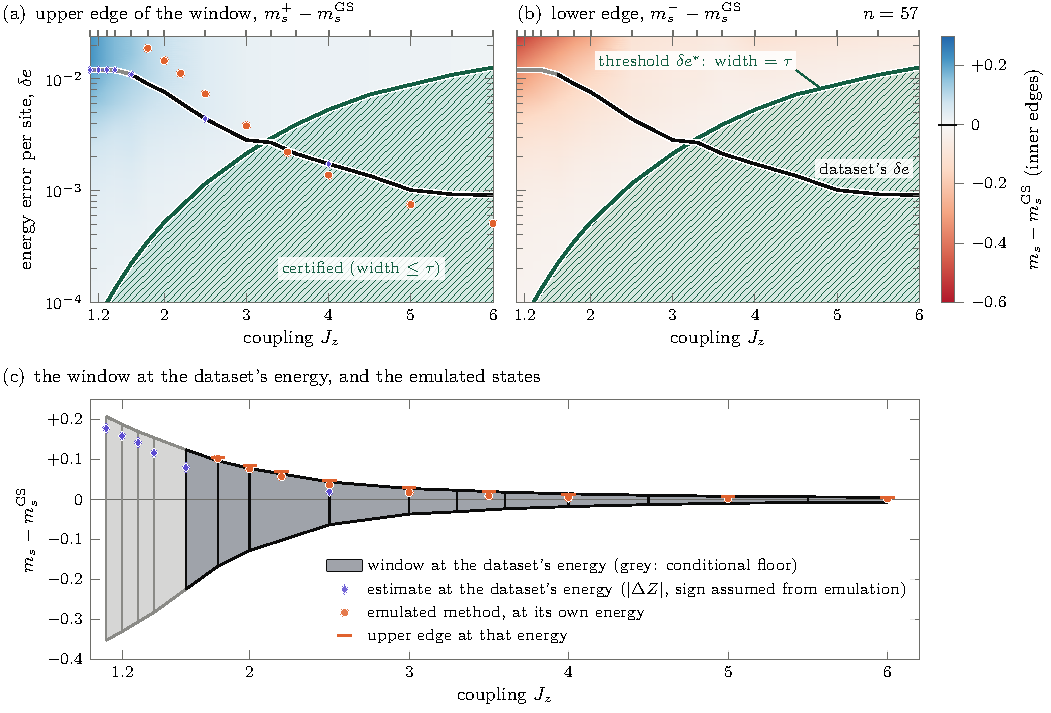
\includegraphics[width=\textwidth]{figS_landscape_n57_pgf}%
\caption{\label{fig:landscape57}The full certification landscape at $n=57$, for sector states and with the digitized % src: file:phase3/full_runs/map/RESULTS.md; def:phase3/full_runs/map/DECLARATION.md
energies (the figures-based map). (a), (b) Colour: the highest and
lowest $\ms$ (relative to the ground-state value) of any sector state with energy error per site at most $\de$
(inner side, from the stored states); their difference is the width shown in Fig.~2(a) of the main % src: file:phase3/full_runs/map/RESULTS.md; def:phase3/full_runs/map/DECLARATION.md
text. Green, hatched: certified, i.e.\ width $\le\tau$ ($\de\le\des(\Jz)$, below the dark green line); black line: the dataset's digitized energy error (grey: conditional floor). (c) Dark % src: file:phase3/full_runs/map/RESULTS.md; def:phase3/full_runs/map/DECLARATION.md
band: the window at the dataset's digitized energy error (grey: conditional floor at the out-of-distribution points).
Orange: emulated method-class states at their own energy (only those inside the plotted range, $\Jz\ge1.8$; dash: the upper edge at that energy; positions in (a)); violet: % src: file:phase3/full_runs/map/RESULTS.md; def:phase3/full_runs/map/DECLARATION.md
an estimate made before the public record was known, at the dataset's energy and from its published unsigned
$\Delta Z$, \emph{with the sign assumed from the emulation}; the public $\ms$ labels have since been found above the
reference at all $100$ points (Sec.~\ref{sm:public}). Both sit on the ``$+$'' side, close to the % src: file:phase3/full_runs/real_data/RESULTS.md (positive at all 100)
upper edge where the bias is large (orange at $0.76$--$0.98$ of it for $\Jz\le2.5$, violet at $0.64$--$0.86$ for % src: figures/pgf_sm_3d/export_check.txt (orange ratios 0.76-0.98 at J <= 2.5, 0.29-0.59 above; violet 0.64-0.86 at J <= 1.6, 0.45 and 0.34 at 2.5 and 4)
$\Jz\le1.6$) and further below it at larger $\Jz$ (down to $0.29$). The $\de$ range stops at $0.024$, the highest stored energy common to all couplings; the maps are straight % src: file:phase3/full_runs/map/RESULTS.md; def:phase3/full_runs/map/DECLARATION.md; derived: highest stored window energy common to all couplings, printed by figures/fig_landscape.py
between computed couplings (ticks on the top axes). Source: deposited map and method outputs.}
\end{figure}


\subsection{Figures-based map at a glance}
The full tables of that map (widths, status under both readings, robustness fractions and the accuracy law, row by row)
are in the ancillary file \texttt{tables.pdf} (Tables~A1--A5); they are generated from the deposited map outputs by a % src: file:phase3/full_runs/map/RESULTS.md; def:phase3/full_runs/map/DECLARATION.md
script of the deposit, which also checks every cell against the deposited Markdown tables of the map (2145 cells, no % src: file:phase3/full_runs/map/RESULTS.md; def:phase3/full_runs/map/DECLARATION.md; file:paper/figures/FIGURES_README.md (2145 map cells)
difference). Table~\ref{tab:map_glance} gives the status of every computed row; Table~\ref{tab:map_jstar} the
thresholds.

\def\SMcap{Figures-based map (sector states, digitized energies): status of every computed row (reading~1; windows of Sec.~\ref{sm:figmodel}). % src: file:phase3/full_runs/map/RESULTS.md; def:phase3/full_runs/map/DECLARATION.md
\textbf{R}: certified (width $\le\tau$; the label is within $\tau$ of the ground-state value), with the lower bounds on the ground energies of the % src: file:phase3/full_runs/map/RESULTS.md; def:phase3/full_runs/map/DECLARATION.md
tilted Hamiltonians proved in exact arithmetic (Sec.~\ref{sm:rigor}; the window threshold $E_{\rm up}$ and the tolerance $\tau$ still use our DMRG reference); C: certified, with DMRG-referenced outer bounds (not tested rigorously);
C$^{*}$: certified with DMRG references, but the rigorous width is $1.09\,\tau$; N: not certified (rigorous: explicit % src: file:phase3/full_runs/map/RESULTS.md; def:phase3/full_runs/map/DECLARATION.md; rig:rows[n=57,Jz=3.4,label=m_s].w_over_tau
states); G: gray zone; $\cdot$: not computed. $^\dagger$: out-of-distribution point (conditional floor
$\epsilon_{\rm dig}=0.012\,n$). Widths, reading~2 and robustness fractions of every row: ancillary Tables~A1--A4.}\def\SMlab{tab:map_glance} % src: file:phase3/full_runs/map/RESULTS.md; def:phase3/full_runs/map/DECLARATION.md
% generated by figures/make_sm_new.py from phase3/full_runs/map/laptop_analysis/summary_map.json (status), phase3/full_runs/rigor/outputs/results_v2.json (rigorous rows) -- do not edit
{\footnotesize\setlength{\tabcolsep}{5pt}\renewcommand{\arraystretch}{1.3}
\needspace{295pt}
\begin{longtable}{@{}lcccccccccccccccccc@{}}
\caption{\SMcap}\label{\SMlab}\\
\toprule
Label & 1.1$^{\dagger}$ & 1.2$^{\dagger}$ & 1.3$^{\dagger}$ & 1.4$^{\dagger}$ & 1.6 & 1.8 & 2.0 & 2.5 & 3.0 & 3.2 & 3.3 & 3.4 & 3.6 & 4.0 & 4.5 & 5.0 & 5.5 & 6.0 \\
\midrule
\multicolumn{19}{@{}l}{\textbf{$n=57$}}\\
$m_s$ & N & N & N & N & N & N & N & N & N & G & G & C$^{*}$ & \textbf{R} & \textbf{R} & \textbf{R} & \textbf{R} & \textbf{R} & \textbf{R} \\
$\bar C_{zz}$ & N & N & N & N & N & N & N & N & N & G & G & \textbf{R} & \textbf{R} & \textbf{R} & \textbf{R} & \textbf{R} & \textbf{R} & \textbf{R} \\
$\bar C_{2}$ & N & N & N & N & N & N & N & N & N & $\cdot$ & N & $\cdot$ & N & G & C & C & C & C \\
$Z_{\rm bulk}$ & N & N & N & N & N & N & N & N & N & $\cdot$ & N & $\cdot$ & N & N & N & N & G & G \\
$Z_{\rm bdry}$ & N & N & N & N & N & N & N & N & N & $\cdot$ & N & $\cdot$ & N & N & N & N & N & G \\
$C_{zz}^{\rm edge}$ & N & N & N & N & N & N & N & N & N & $\cdot$ & N & $\cdot$ & N & N & N & N & G & G \\
$Z_{\rm loop}$ & N & N & N & N & N & N & N & N & N & $\cdot$ & N & $\cdot$ & N & N & N & N & N & N \\
\multicolumn{19}{@{}l}{\textbf{$n=115$}}\\
$m_s$ & N & N & N & N & N & N & N & N & G & $\cdot$ & C & $\cdot$ & C & \textbf{R} & C & C & C & \textbf{R} \\
$\bar C_{zz}$ & N & N & N & N & N & N & N & N & G & $\cdot$ & C & $\cdot$ & C & \textbf{R} & C & C & C & \textbf{R} \\
$\bar C_{2}$ & N & N & N & N & N & N & N & N & N & $\cdot$ & N & $\cdot$ & G & C & C & C & C & C \\
$Z_{\rm bulk}$ & $\cdot$ & $\cdot$ & $\cdot$ & $\cdot$ & $\cdot$ & $\cdot$ & $\cdot$ & $\cdot$ & $\cdot$ & $\cdot$ & $\cdot$ & $\cdot$ & $\cdot$ & N & $\cdot$ & $\cdot$ & $\cdot$ & $\cdot$ \\
\bottomrule
\end{longtable}
}


\def\SMcap{Figures-based map: certification thresholds per label and size. $J^*$ is the smallest training coupling from which every
larger training point ($\Jz=1.6,1.7,\dots,6.0$, 45 points) is certified, with $\epsilon_\tau$ interpolated % src: file:phase3/full_runs/map/RESULTS.md; def:phase3/full_runs/map/DECLARATION.md
log-linearly between computed couplings. \emph{Central}: certified at the digitized error $\epsilon_{\rm dig}$;
\emph{20\,\% margin}: certified at $1.2\,\epsilon_{\rm dig}$ (with the larger of our and the dataset's gaps); the last % src: file:phase3/full_runs/map/RESULTS.md; def:phase3/full_runs/map/DECLARATION.md
two columns repeat the central threshold with the independent reading 2, which has no value at $\Jz=5.1$ ($n=57$) and % src: file:phase3/full_runs/map/RESULTS.md; def:phase3/full_runs/map/DECLARATION.md
therefore counts one point less. \emph{none}: no threshold within the training
range.}\def\SMlab{tab:map_jstar}
% generated by figures/make_sm_tables.py from phase3/full_runs/map/laptop_analysis/summary_map.json (jstar); same values as phase3/full_runs/map/laptop_analysis/tables_map.md -- do not edit
{\footnotesize\setlength{\tabcolsep}{5pt}\renewcommand{\arraystretch}{1.3}
\needspace{298pt}
\begin{longtable}{lcccccc}
\caption{\SMcap}\label{\SMlab}\\
\toprule
 & \multicolumn{2}{c}{threshold $J^*$} & \multicolumn{2}{c}{certified training points (of 45)} & \multicolumn{2}{c}{reading 2} \\ \cmidrule(lr){2-3}\cmidrule(lr){4-5}\cmidrule(l){6-7}
Label & central & 20\,\% margin & central & 20\,\% margin & $J^*$ & certified \\
\midrule
\multicolumn{7}{@{}l}{\textbf{$n=57$}}\\
$m_s$ & 3.2 & 3.4 & 29 & 27 & 3.2 & 28 \\
$\bar C_{zz}$ & 3.2 & 3.4 & 29 & 27 & 3.2 & 28 \\
$\bar C_{2}$ & 4.0 & 4.2 & 21 & 19 & 4.0 & 20 \\
$Z_{\rm bulk}$ & 6.0 & \textit{none} & 1 & 0 & 6.0 & 1 \\
$Z_{\rm bdry}$ & \textit{none} & \textit{none} & 0 & 0 & \textit{none} & 0 \\
$C_{zz}^{\rm edge}$ & 6.0 & \textit{none} & 1 & 0 & 6.0 & 1 \\
$Z_{\rm loop}$ & \textit{none} & \textit{none} & 0 & 0 & \textit{none} & 0 \\
\multicolumn{7}{@{}l}{\textbf{$n=115$}}\\
$m_s$ & 3.1 & 3.3 & 30 & 28 & 3.1 & 30 \\
$\bar C_{zz}$ & 3.1 & 3.3 & 30 & 28 & 3.1 & 30 \\
$\bar C_{2}$ & 3.8 & 3.9 & 23 & 22 & 3.8 & 23 \\
\bottomrule
\end{longtable}
}



\needspace{0.55\textheight} % (layout)
\subsection{Figures-based map: consistency checks}
\def\SMcap{Consistency checks of the figures-based map computation, all fixed before the run. Each row names the check and what it
covers, whether it passed, and the measured deviations (energies in units of the exchange coupling). The last row is a
record kept for comparison, not a pass condition; it is recomputed here from the stored record of the map.}\def\SMlab{tab:map_checks}
% generated by figures/sm_tables/make_rdmap.py: figures/sm_tables/map_checks.tex with its last row recomputed from phase3/full_runs/map/laptop_analysis/summary_map.json (gates.G3_gap_record) -- do not edit
{\footnotesize\setlength{\tabcolsep}{5pt}\renewcommand{\arraystretch}{1.3}
\needspace{490pt}
\begin{longtable}{lll}
\caption{\SMcap}\label{\SMlab}\\
\toprule
Check and scope & Result & Detail \\
\midrule
\parbox[t]{150pt}{\raggedright\strut\textbf{Exact diagonalization at $n=19$}\\ $m_s$, $\bar C_{zz}$, $Z_{\rm bulk}$ at $J_z$ = 1.6, 4.0\strut} & \parbox[t]{52pt}{\raggedright\strut passed\strut} & \parbox[t]{270pt}{\raggedright\strut outer width within 0.43 \% of exact at $E_{\rm lo}$, $E_{\rm dig}$, $E_{\rm up}$; inner within 0.12 \% at $E_{\rm lo}$, 0.58 \% at $E_{\rm dig}$, $E_{\rm up}$; $\epsilon_\tau$ (inner and outer) within 0.25 \%\strut} \\
\parbox[t]{150pt}{\raggedright\strut\textbf{Higher reference bond dimension}\\ bond dimension 320 $\to$ 480, $n={}$57, $J_z$ = 1.2, 1.6, 3.3, 4.0, 6.0\strut} & \parbox[t]{52pt}{\raggedright\strut passed\strut} & \parbox[t]{270pt}{\raggedright\strut $|\Delta E_0|$ = $3.5\times10^{-6}$, $2.8\times10^{-7}$, $8.8\times10^{-11}$, $8.7\times10^{-12}$, $1.4\times10^{-13}$ (limits 0.016--0.0013)\strut} \\
\parbox[t]{150pt}{\raggedright\strut\textbf{Outer-bound energies at bond dimension 160}\\ G at bond dimension 160 vs 320 at the decisive $\lambda$; $n={}$57, 115; $J_z$ = 3.3, 4.0; $m_s$, $\bar C_{zz}$; $\pm$\strut} & \parbox[t]{52pt}{\raggedright\strut passed\strut} & \parbox[t]{270pt}{\raggedright\strut $|\Delta G|$ $\le$ $9.0\times10^{-5}$ ($n={}$115, 3.3, $m_s$ $-$) against limits $1.2\times10^{-3}$ to $3.4\times10^{-3}$; $\le$ $4.9\times10^{-7}$ at $n={}$57\strut} \\
\parbox[t]{150pt}{\raggedright\strut\textbf{Cold against warm starts}\\ cold starts, $m_s$ $\pm$, same points\strut} & \parbox[t]{52pt}{\raggedright\strut passed\strut} & \parbox[t]{270pt}{\raggedright\strut $F_{\rm cold}-F_{\rm warm}$ $\in$ [$3\times10^{-12}$, $4.6\times10^{-5}$], no warm start stuck\strut} \\
\parbox[t]{150pt}{\raggedright\strut\textbf{Sector and evaluators}\\ 2680 stored states of the sector\strut} & \parbox[t]{52pt}{\raggedright\strut passed\strut} & \parbox[t]{270pt}{\raggedright\strut 0 out of sector, variance 0, TeNPy vs evaluator $|\Delta E|$ $\le$ $2.6\times10^{-12}$, $|\Delta m_s|$ $\le$ $3.9\times10^{-12}$\strut} \\
\parbox[t]{150pt}{\raggedright\strut\textbf{Separate-process re-evaluation}\\ separate process, TeNPy not importable; 508 headline components of $m_s$ and $\bar C_{zz}$ at every $J_z$, both sizes, and $Z_{\rm bulk}$\strut} & \parbox[t]{52pt}{\raggedright\strut passed\strut} & \parbox[t]{270pt}{\raggedright\strut $|\Delta E|$ $\le$ $1.8\times10^{-12}$, $|\Delta(\text{label})|$ = 0, $|\Delta(\text{norm})|/\text{norm}$ $\le$ $8\times10^{-15}$, variance 0; every mixture and pure witness below its threshold; none missing\strut} \\
\parbox[t]{150pt}{\raggedright\strut \textbf{Gap against the dataset's (recorded, not a pass condition)}\\ our $S^z=s-1$ gap vs the dataset's\strut} & \parbox[t]{52pt}{\raggedright\strut 66/68 within 10 \%\strut} & \parbox[t]{270pt}{\raggedright\strut within 0.81 \% at every computed training coupling (both readings) except $n={}$57, $J_z$ = 1.6, where the dataset's marker is partly covered: +4.1 \% (reading 1) and +5.1 \% (reading 2); $n={}$115, $J_z$ = 1.1: +20.5 \% and +21.2 \%, 1.2: +6.9 \% and +7.0 \% (our bond dimension $\le$ 200 reference is under-converged there; the thresholds at the test couplings do not use the gap)\strut} \\
\bottomrule
\end{longtable}
}


\noindent The $n=115$ reference at $\Jz\le1.2$ (bond dimension $\le200$ for the gap states) is probably % src: file:phase3/full_runs/map/RESULTS.md; def:phase3/full_runs/map/DECLARATION.md
under-converged; the OOD windows do not use the gap. At $n=115$, $\Jz\le1.4$ the computed $\epsilon_\tau$ % src: file:phase3/full_runs/map/RESULTS.md; def:phase3/full_runs/map/DECLARATION.md
($\approx0.003$--$0.03$) is comparable to the offset of the bond-dimension-160 chain states, so the law check is not % src: file:phase3/full_runs/map/RESULTS.md; def:phase3/full_runs/map/DECLARATION.md
resolved there. At $n=57$, $\Jz=1.6$, where the dataset's gap marker is partly covered, our gap is $4.1\%$ (reading 1) % src: map:gates.G3_gap_record.rows (rel 0.0408 with reading 1 and 0.0509 with reading 2, n = 57, Jz = 1.6)
and $5.1\%$ (reading 2) above the reading; the witness side uses the smaller and the certificate side the larger of % src: map:gates.G3_gap_record.rows (rel 0.0509)
the two gaps. The cold starts of the fourth row begin from the N\'eel state and therefore test the N\'eel-like branch
only: on the ``$-$'' side of $\ms$ they cannot exclude a lower reversed-domain state, a question that the exact
lower bounds of Sec.~\ref{sm:rigor} close where they exist.

\subsection{Pure and minimal-bond-dimension witnesses}
\label{sm:pure}

\emph{Pure witnesses.} The two mixture witnesses of $\ms$ at $n=57$, $\Jz=1.6$, $E_{\rm lo}=E_0+0.4990$ were turned into % src: file:phase3/full_runs/map/RESULTS.md; def:phase3/full_runs/map/DECLARATION.md
single pure states by the construction of Lemma~B from the stored matrix-product states and re-evaluated with the
independent code (Table~\ref{tab:map_th_witness}). The width from $0.5765$ to $0.8846$ ($D=0.3081$) is attained by two explicit pure sector states % src: map:row(57,1.6,m_s).at_lo.inner; map:row(57,1.6,m_s).at_lo.inner; map:row(57,1.6,m_s).at_lo.w_in
below the threshold; the larger has bond dimension $320$. The best single stored states, without superposition, % src: file:phase3/full_runs/map/RESULTS.md; def:phase3/full_runs/map/DECLARATION.md
reach $0.3049$ of the $0.3081$, that is $98.9\%$ of the width. % src: map:row(57,1.6,m_s).at_lo.w_pure (0.3049); map:row(57,1.6,m_s).at_lo.w_in (0.3081); derived: 0.3049/0.3081 = 0.9897, rounded down

\def\SMcap{The two explicit pure witnesses of $\ms$ at $n=57$, $\Jz=1.6$ (Lemma~B). Each column is one end of the % src: file:phase3/full_runs/map/RESULTS.md; def:phase3/full_runs/map/DECLARATION.md
window: the pure state $\alpha|a\rangle+\beta|b\rangle$ built from two stored matrix-product states $|a\rangle$,
$|b\rangle$, with $(\alpha,\beta)$ from the $2\times2$ compression of $(H,\ms)$ to their span. Read down a column: the % src: file:phase3/full_runs/map/RESULTS.md; def:phase3/full_runs/map/DECLARATION.md
pure state has the energy and the label of the mixture it replaces, lies in the sector, and is below the threshold
$E_{\rm lo}$. Energies in units of the exchange coupling.}\def\SMlab{tab:map_th_witness}
% generated by figures/make_sm_tables.py from phase3/full_runs/map/RESULTS.md Sec. 8 -- do not edit
{\footnotesize\setlength{\tabcolsep}{5pt}\renewcommand{\arraystretch}{1.3}
\needspace{334pt}
\begin{longtable}{lll}
\caption{\SMcap}\label{\SMlab}\\
\toprule
Quantity & lower end $\phi_-$ & upper end $\phi_+$ \\
\midrule
\parbox[t]{150pt}{\raggedright\strut two stored components ($\lambda$, bond dimension)\strut} & \parbox[t]{150pt}{\raggedright\strut $m_s$ ``$-$'' chain, $\lambda$ = 0.066484 and 0.074994 (bond dimension 160 each)\strut} & \parbox[t]{150pt}{\raggedright\strut minimal-$\chi$ runs, $\lambda$ = 0.194440 and 0.196557 (bond dimension 64 each)\strut} \\
\parbox[t]{150pt}{\raggedright\strut weight of the first component in the mixture\strut} & 0.8391 & 0.2813 \\
\parbox[t]{150pt}{\raggedright\strut overlap $\langle a|b\rangle$\strut} & 0.9749 & 0.99999 \\
\parbox[t]{150pt}{\raggedright\strut bond dimension of the pure state\strut} & 320 & 128 \\
\parbox[t]{150pt}{\raggedright\strut $\langle H\rangle-E_{\rm mix}$ (pure minus mixture energy)\strut} & +$1.4\times10^{-14}$ & $-4.9\times10^{-13}$ \\
\parbox[t]{150pt}{\raggedright\strut $m_s$ of the pure state ($=$ mixture)\strut} & 0.5765 & 0.8846 \\
\parbox[t]{150pt}{\raggedright\strut variance of the sector charge\strut} & 0 & 0 \\
\parbox[t]{150pt}{\raggedright\strut energy below $E_{\rm lo}$\strut} & yes (by $1.0\times10^{-6}$) & yes \\
\bottomrule
\end{longtable}
}


\emph{Minimal bond dimension.} Rerunning the extremal chains at bond dimension $16$, $32$ and $64$ (cold starts) shows % src: file:phase3/full_runs/map/RESULTS.md; def:phase3/full_runs/map/DECLARATION.md
how simple the extremal states are (Table~\ref{tab:map_minchi}).

\def\SMcap{Minimal-bond-dimension witnesses: the extremal chains rerun at small bond dimension (cold starts).
$E_0(\text{bond dim.})-E_0$: how far the ground energy at that bond dimension lies above the reference; % src: file:phase3/full_runs/map/RESULTS.md; def:phase3/full_runs/map/DECLARATION.md
$D_{\rm pure}$: the width attained by the best two pure states below $E_{\rm lo}$; last column: its fraction of the
pure-state width found at the full bond dimension. Read down a block: bond dimension $32$ already gives almost the full % src: file:phase3/full_runs/map/RESULTS.md; def:phase3/full_runs/map/DECLARATION.md
width.}\def\SMlab{tab:map_minchi}
% generated by figures/make_sm_tables.py from phase3/full_runs/map/laptop_analysis/summary_map.json (minchi) -- do not edit
{\footnotesize\setlength{\tabcolsep}{5pt}\renewcommand{\arraystretch}{1.3}
\needspace{230pt}
\begin{longtable}{cccc}
\caption{\SMcap}\label{\SMlab}\\
\toprule
Bond dimension & $E_0(\text{bond dim.})-E_0$ & $D_{\rm pure}$ & fraction of the full $D_{\rm pure}$ \\
\midrule
\multicolumn{4}{@{}l}{\textbf{$n=57$, $J_z=1.6$, $m_s$}}\\
16 & 0.069\phantom{0} & 0.259\phantom{0} & 0.849 \\
32 & 0.0083 & 0.295\phantom{0} & 0.968 \\
64 & $5.1\times10^{-4}$ & 0.305\phantom{0} & 1.00\phantom{0} \\
\multicolumn{4}{@{}l}{\textbf{$n=57$, $J_z=4.0$, $m_s$}}\\
16 & 0.0029 & 0.0276 & 0.971 \\
32 & $1.3\times10^{-4}$ & 0.0283 & 0.995 \\
64 & $8.8\times10^{-7}$ & 0.0283 & 0.997 \\
\bottomrule
\end{longtable}
}


\section{Rigorous lower bounds on the certified side}
\label{sm:rigor}

\subsection{Method}
The outer bound of Sec.~\ref{sm:proofs} needs, for each field $\lambda$, a lower bound on the energy of
the tilted Hamiltonian $H'=H-\sigma\lambda SO$ over the states considered. With DMRG it is $G_\sigma(\lambda)-\delta G$, for sector states; any rigorous lower bound
$E_{\rm LB}(H')$ can replace it, and then $\sigma\langle O\rangle_\rho\le[E-E_{\rm LB}(H')]/(\lambda S)$ holds for every
such state $\rho$ with $\Tr H\rho\le E$, with no reference (Lemma~A). We obtain $E_{\rm LB}$ from a cluster relaxation in dual
form. Cover the graph by clusters $C_k$ and split $H'=\sum_kh_k$ with each term assigned to a cluster that contains
it. For every pair of overlapping clusters, an $S^z$-preserving operator $Y$ on the overlap may be added to one
cluster term and subtracted from the other, and a multiple $\mu M_k$ of the share of the total magnetization
$M_z=\sum_iZ_i$ in cluster $k$ may be added to each term. Then, as operators on the full space,
\begin{equation}
H'+\mu M_z\ \ge\ \sum_kt_k,\qquad t_k\le\lambda_{\min}\big(h_k+\textstyle\sum Y\text{'s}+\mu M_k\big), % src: file:phase3/full_runs/rigor/RESULTS_v2.md; file:phase3/full_runs/rigor/RESULTS.md; def:phase3/full_runs/rigor/DECLARATION_v2.md
\label{eq:opineq}
\end{equation}
so every state $\rho$ with mean magnetization $\Tr M_z\rho=M$ has
\begin{equation}
\Tr H'\rho\ \ge\ \sum_kt_k-\mu M=:E_{\rm LB}(M). % src: file:phase3/full_runs/rigor/RESULTS_v2.md; def:phase3/full_runs/rigor/DECLARATION_v2.md
\label{eq:elb}
\end{equation}
The bound is the sum of the cluster bounds \emph{minus $\mu$ times the magnetization}; the bare sum of the $t_k$ is
not a bound on the sector energy (for seven of the winning certificates of Table~\ref{tab:rig_v2} it lies above the % src: file:phase3/full_runs/real_data/checks/r11/ft_rigor_mu_table_out.txt (7 of 36)
DMRG energy). Only the mean of $M_z$ enters. With $M=M_0$, Eq.~\eqref{eq:elb} bounds the sector ground energy, which
is how the certificates were used originally; with $M=M_{\rm pub}$ it bounds the tilted energy of the published states,
which are not in the sector (Sec.~\ref{sm:public_sector}), and this is the form behind every ``certified'' status of
the main text (Sec.~\ref{sm:public_exact}). Without $\mu$ the relaxation would bound the ground energy over all
sectors, which for the side that opposes the order is far lower. Maximizing over the
multipliers is the dual of the relaxation in which every cluster carries a density matrix, overlapping clusters
agree on their common marginals and the mean magnetization is fixed. Without the last constraint this is a
local-consistency relaxation over a family of clusters of the kind defined in Ref.~\cite{lin2026} (their Definition~7; % (structural: definition number)
the first level of their hierarchy uses pairwise marginals), and one of their solvers, like ours, works with a
smoothed dual; in dual form it is an optimized Anderson cluster bound~\cite{anderson1951}. What we add is the multiplier of the mean
magnetization, which enters the bound, the exact verification below and the use for labels. The semidefinite
relaxations of Refs.~\cite{barthel2012,baumgratz2012} are of a related local kind reached by another route: they
impose positivity on the expectation values of operators supported on subsets of the lattice (few-particle Green's
functions in Ref.~\cite{barthel2012}, moment matrices in Ref.~\cite{baumgratz2012}), where ours keeps a full density
matrix on every cluster. Two cluster sets were used: % src: file:phase3/full_runs/rigor/RESULTS_v2.md; file:phase3/full_runs/rigor/RESULTS.md; def:phase3/full_runs/rigor/DECLARATION_v2.md
all sites within distance two of an edge (at most nine sites; 62 clusters and 719 overlaps at $n=57$) and radius-two % src: file:phase3/full_runs/rigor/RESULTS_v2.md; file:phase3/full_runs/rigor/RESULTS.md; def:phase3/full_runs/rigor/DECLARATION_v2.md
vertex balls (at most seven sites; 55 clusters at $n=57$, 113 at $n=115$). Each $\lambda_{\min}$ is replaced by a soft % src: file:phase3/full_runs/rigor/RESULTS_v2.md; file:phase3/full_runs/rigor/RESULTS.md; def:phase3/full_runs/rigor/DECLARATION_v2.md
minimum whose sharpness is raised from $30$ to $10^5$ during an L-BFGS optimization. % src: file:phase3/full_runs/rigor/RESULTS_v2.md; file:phase3/full_runs/rigor/RESULTS.md; def:phase3/full_runs/rigor/DECLARATION_v2.md

\emph{Certificate.} The optimized multipliers are rounded to dyadic rationals ($2^{-32}$). For every cluster the bound % src: file:phase3/full_runs/rigor/RESULTS_v2.md; file:phase3/full_runs/rigor/RESULTS.md; def:phase3/full_runs/rigor/DECLARATION_v2.md
$t_k$ is proved by showing that $h_k-t_k$ (with the rounded multipliers, scaled to integers) is positive definite on
every $S^z$ block by exact integer (Bareiss) elimination, in a separate program that uses only Python integers and does
not import the optimizer ($406$ blocks per vertex-ball certificate and $568$ per edge-ball certificate at $n=57$, the % src: file:phase3/full_runs/rigor/RESULTS_v2.md; file:phase3/full_runs/real_data/checks/r11/ft_rigor_block_counts_out.txt (406, 35; 568, 126)
greatest $126\times126$; $854$ at $n=115$). The sum of the verified % src: file:phase3/full_runs/rigor/RESULTS_v2.md; file:phase3/full_runs/real_data/checks/r11/ft_rigor_block_counts_out.txt (568, 126; 854, 35)
$t_k$, minus $\mu M$, is the certified $E_{\rm LB}(M)$. The verifier rejects a tampered certificate in its tests. Rounding an
inexact dual solution and verifying it in exact arithmetic follows the rational post-processing of Ref.~\cite{naceur2025}, which builds on rounding-and-projection schemes for sums of squares; bounding observables % src: file:phase3/full_runs/rigor/RESULTS_v2.md; file:phase3/full_runs/rigor/RESULTS.md; def:phase3/full_runs/rigor/DECLARATION_v2.md
from a relaxation lower bound and an energy constraint is that of the ground-state certificates of
Refs.~\cite{wang2024prx,wang2026scipost}, there with semidefinite relaxations. % src: file:phase3/full_runs/rigor/RESULTS_v2.md; file:phase3/full_runs/rigor/RESULTS.md; def:phase3/full_runs/rigor/DECLARATION_v2.md

\emph{Declared grid and decision.} The certificates were computed for the figures-based map (Sec.~\ref{sm:figmap}),
at its certificate-side windows $E_{\rm up}$ and for sector states. For every row, side and size, the declared grid was every $\lambda$ of the stored
chain plus $\lambda_{\rm dec}0.85^k$, $k=1,2,3$, with $\lambda_{\rm dec}$ the chain point decisive for the % src: file:phase3/full_runs/rigor/RESULTS_v2.md; file:phase3/full_runs/rigor/RESULTS.md; def:phase3/full_runs/rigor/DECLARATION_v2.md
DMRG-referenced bound at $E_{\rm up}$; points that provably cannot lead to a certified width were pruned, and a
branch-and-bound over the rest stopped each side when no remaining point could improve its bound by more than
$0.01\,\tau$. The % src: def:phase3/full_runs/real_data/e1/E1_SPEC.md (a side stops when the next point is within 0.01 tau of the best)
rigorous width $w_{\rm rig}$ is the sum over the two sides of the best verified bound. A row is certified if
$w_{\rm rig}\le\tau$; per block of rows the decision rule fixed in advance used $\rho=(w_{\rm rig}-w_{\rm
DMRG})/(\tau-w_{\rm DMRG})$: confirmed if $\max\rho\le1$, rejected if $\max\rho\ge3$. Calibration: at $n=19$ all 24 % src: file:phase3/full_runs/rigor/RESULTS_v2.md; file:phase3/full_runs/rigor/RESULTS.md; def:phase3/full_runs/rigor/DECLARATION_v2.md
bounds of this grid lie below the exact sector ground energies (true slack $0.0002$--$0.029$, the greatest at the % src: file:phase3/full_runs/rigor/RESULTS_v2.md; file:phase3/full_runs/rigor/RESULTS.md; def:phase3/full_runs/rigor/DECLARATION_v2.md
``$-$'' points of $\ms$ next to a level crossing).

\subsection{Results at the figures-based windows}
\def\SMcap{Rigorous certificates at the computed points where the figures-based map certifies $\ms$ and $\Czz$ ($n=57$: all % src: file:phase3/full_runs/rigor/RESULTS_v2.md; file:phase3/full_runs/rigor/RESULTS.md; def:phase3/full_runs/rigor/DECLARATION_v2.md
of them; $n=115$: $\Jz=4.0$ and $6.0$). Proved interval: the values of the label allowed, for sector states, by the energy window at % src: file:phase3/full_runs/rigor/RESULTS_v2.md; file:phase3/full_runs/rigor/RESULTS.md; def:phase3/full_runs/rigor/DECLARATION_v2.md
$E_{\rm up}$ (the certificate-side window of Sec.~\ref{sm:figmodel}), proved with exact lower bounds, ends rounded outward; $w_{\rm rig}/\tau$ its
width over the reference tolerance and $w_{\rm rig}/\tau_{\rm rf}$ over the reference-free tolerance ($6\%$ of the smaller end of the interval in absolute value), both rounded up; $w_{\rm DMRG}/\tau$ the DMRG-referenced width at the same window. Slack: DMRG energy minus verified lower bound % src: derived: 0.06 times the smaller end of the proved interval in absolute value
at the winning field of each side (units of the exchange coupling; an upper bound on the true slack). Bold $\Jz$:
within $\tau$. For the public labels these rows are superseded by the intervals of Sec.~\ref{sm:public_exact}.}\def\SMlab{tab:rig_v2} % src: file:phase3/full_runs/rigor/RESULTS_v2.md; file:phase3/full_runs/rigor/RESULTS.md; def:phase3/full_runs/rigor/DECLARATION_v2.md
% generated by figures/sm_tables/make_rdmap.py from phase3/full_runs/rigor/outputs/results_v2.json (rows: interval, w_cert, tau, w_F, sides) -- do not edit
{\footnotesize\setlength{\tabcolsep}{5pt}\renewcommand{\arraystretch}{1.2}
\needspace{346pt}
\begin{longtable}{@{}llccccll@{}}
\caption{\SMcap}\label{\SMlab}\\
\toprule
$J_z$ & Label & proved interval at $E_{\rm up}$ & $w_{\rm rig}/\tau$ & $w_{\rm rig}/\tau_{\rm rf}$ & $w_{\rm DMRG}/\tau$ & slack $+$ / $-$ & status \\
\midrule
\multicolumn{8}{@{}l}{\rule[-3pt]{0pt}{11.5pt}\textbf{$n=57$}}\\
\rule[-3pt]{0pt}{11.5pt} 3.4 & $m_s$ & $[0.90479,\,0.96624]$ & 1.086 & 1.132 & 0.958 & 0.0016 / 0.039 & wider than $\tau$ \ding{55} \\
\rule[-3pt]{0pt}{11.5pt} \textbf{3.4} & $\bar C_{zz}$ & $[-0.96245,\,-0.90646]$ & 0.995 & 1.030 & 0.953 & 0.023 / 0.0030 & within $\tau$ \ding{51} \\
\rule[-3pt]{0pt}{11.5pt} \textbf{3.6} & $m_s$ & $[0.91720,\,0.96898]$ & 0.910 & 0.941 & 0.809 & 0.0014 / 0.027 & within $\tau$ \ding{51} \\
\rule[-3pt]{0pt}{11.5pt} \textbf{3.6} & $\bar C_{zz}$ & $[-0.96545,\,-0.91755]$ & 0.846 & 0.871 & 0.814 & 0.016 / 0.0026 & within $\tau$ \ding{51} \\
\rule[-3pt]{0pt}{11.5pt} \textbf{4.0} & $m_s$ & $[0.93593,\,0.97394]$ & 0.661 & 0.677 & 0.610 & 0.0012 / 0.020 & within $\tau$ \ding{51} \\
\rule[-3pt]{0pt}{11.5pt} \textbf{4.0} & $\bar C_{zz}$ & $[-0.97092,\,-0.93359]$ & 0.652 & 0.667 & 0.625 & 0.015 / 0.0024 & within $\tau$ \ding{51} \\
\rule[-3pt]{0pt}{11.5pt} \textbf{4.5} & $m_s$ & $[0.95008,\,0.97864]$ & 0.493 & 0.501 & 0.446 & 0.00090 / 0.021 & within $\tau$ \ding{51} \\
\rule[-3pt]{0pt}{11.5pt} \textbf{4.5} & $\bar C_{zz}$ & $[-0.97610,\,-0.94836]$ & 0.480 & 0.488 & 0.465 & 0.0083 / 0.0017 & within $\tau$ \ding{51} \\
\rule[-3pt]{0pt}{11.5pt} \textbf{5.0} & $m_s$ & $[0.96140,\,0.98188]$ & 0.351 & 0.355 & 0.325 & 0.00074 / 0.013 & within $\tau$ \ding{51} \\
\rule[-3pt]{0pt}{11.5pt} \textbf{5.0} & $\bar C_{zz}$ & $[-0.97969,\,-0.95923]$ & 0.352 & 0.356 & 0.343 & 0.0051 / 0.0014 & within $\tau$ \ding{51} \\
\rule[-3pt]{0pt}{11.5pt} \textbf{5.5} & $m_s$ & $[0.96831,\,0.98503]$ & 0.285 & 0.288 & 0.267 & 0.0017 / 0.0096 & within $\tau$ \ding{51} \\
\rule[-3pt]{0pt}{11.5pt} \textbf{5.5} & $\bar C_{zz}$ & $[-0.98318,\,-0.96622]$ & 0.290 & 0.293 & 0.283 & 0.0034 / 0.0021 & within $\tau$ \ding{51} \\
\rule[-3pt]{0pt}{11.5pt} \textbf{6.0} & $m_s$ & $[0.97346,\,0.98759]$ & 0.240 & 0.242 & 0.232 & 0.0015 / 0.0062 & within $\tau$ \ding{51} \\
\rule[-3pt]{0pt}{11.5pt} \textbf{6.0} & $\bar C_{zz}$ & $[-0.98599,\,-0.97124]$ & 0.251 & 0.253 & 0.247 & 0.0024 / 0.00097 & within $\tau$ \ding{51} \\
\multicolumn{8}{@{}l}{\rule[-3pt]{0pt}{11.5pt}\textbf{$n=115$}}\\
\rule[-3pt]{0pt}{11.5pt} \textbf{4.0} & $m_s$ & $[0.94198,\,0.97365]$ & 0.550 & 0.561 & 0.486 & 0.0029 / 0.053 & within $\tau$ \ding{51} \\
\rule[-3pt]{0pt}{11.5pt} \textbf{4.0} & $\bar C_{zz}$ & $[-0.97001,\,-0.93894]$ & 0.542 & 0.552 & 0.516 & 0.026 / 0.0054 & within $\tau$ \ding{51} \\
\rule[-3pt]{0pt}{11.5pt} \textbf{6.0} & $m_s$ & $[0.97753,\,0.98658]$ & 0.154 & 0.155 & 0.144 & 0.0036 / 0.0096 & within $\tau$ \ding{51} \\
\rule[-3pt]{0pt}{11.5pt} \textbf{6.0} & $\bar C_{zz}$ & $[-0.98454,\,-0.97494]$ & 0.164 & 0.165 & 0.159 & 0.0039 / 0.0022 & within $\tau$ \ding{51} \\
\bottomrule
\end{longtable}
}


For each of the eighteen rows (nine coupling--size pairs, two labels each) the lower bounds prove an interval that
contains the label of every sector state of energy at most $E_{\rm up}$. In seventeen rows the proved interval is at
most $\tau$ wide; the threshold $E_{\rm up}$ of the window and the tolerance $\tau$ still use our DMRG reference and the
digitized energy (Sec.~\ref{sm:figmodel}). With the reference-free tolerance the count is $16$: the $\Czz$ row at % src: derived: recount of the column w_rig/tau_rf of the table, generated from rig:rows
$\Jz=3.4$ then stands at $1.030$. The rigorous % src: derived: 0.0559865/(0.06 x 0.906461) = 1.0294, rounded up; rig:rows[n=57,Jz=3.4,label=Czz_bar].interval
widths exceed the DMRG-referenced ones by $0.004$--$0.10\,\tau$ on the seventeen rows. The exception is $\ms$ at % src: file:phase3/full_runs/rigor/RESULTS_v2.md; file:phase3/full_runs/rigor/RESULTS.md; def:phase3/full_runs/rigor/DECLARATION_v2.md
$\Jz=3.4$, whose DMRG-referenced width is already $0.958\,\tau$; its rigorous width is $1.09\,\tau$. The $\Czz$ row at % src: file:phase3/full_runs/rigor/RESULTS_v2.md; file:phase3/full_runs/rigor/RESULTS.md; def:phase3/full_runs/rigor/DECLARATION_v2.md
$\Jz=3.4$ is within $\tau$ at $0.995\,\tau$, inside the $0.02\,\tau$ tolerance of the search (two sides), so its margin is thin. By the % src: rig:rows[n=57,Jz=3.4,label=Czz_bar].w_over_tau (0.99448); file:phase3/full_runs/rigor/RESULTS_v2.md; derived: 0.99448 rounded up
rule fixed in advance, the blocks $n=57$, $\Jz=4.0$ and $6.0$ ($\max\rho=0.13$) and $n=115$, $\Jz=4.0$ and $6.0$ % src: file:phase3/full_runs/rigor/RESULTS_v2.md; file:phase3/full_runs/rigor/RESULTS.md; def:phase3/full_runs/rigor/DECLARATION_v2.md
($0.12$) are confirmed, and the block $n=57$, $\Jz=3.4$--$5.5$ is rejected ($\max\rho=3.05$, decided by the $\ms$ row % src: file:phase3/full_runs/rigor/RESULTS_v2.md; file:phase3/full_runs/rigor/RESULTS.md; def:phase3/full_runs/rigor/DECLARATION_v2.md
at $\Jz=3.4$): one of the three declared blocks is rejected. The relaxation is tight to $\le0.05\%$ of $|E|$ on the ``$+$'' sides and for $\Czz$ and to $\le0.08\%$ at % src: file:phase3/full_runs/rigor/RESULTS_v2.md; file:phase3/full_runs/real_data/checks/r11/ft_rigor_mu_table_out.txt (0.0763%; 0.0480 %); derived: rounded up
the winning ``$-$'' fields of $\ms$, which lie below the reversed-domain crossing of the ``$-$'' chains; next to that crossing it loses about $2\%$. At $n=115$ a % src: file:phase3/full_runs/rigor/RESULTS_v2.md; file:phase3/full_runs/rigor/RESULTS.md; def:phase3/full_runs/rigor/DECLARATION_v2.md
certificate took $6.3$ minutes (median), $1.4$ times the time at $n=57$ for twice the sites; the verification is per % src: file:phase3/full_runs/rigor/RESULTS_v2.md; file:phase3/full_runs/rigor/RESULTS.md; def:phase3/full_runs/rigor/DECLARATION_v2.md
cluster and scales linearly. All 135 certificates of this run were verified exactly, with no failure. % src: file:phase3/full_runs/rigor/RESULTS_v2.md; file:phase3/full_runs/rigor/RESULTS.md; def:phase3/full_runs/rigor/DECLARATION_v2.md

\subsection{An earlier test, rejected}
Before the grid run, a test with one field per side fixed in advance (the chain points decisive at $E_{\rm up}$ plus
the greatest admissible slack) was run at $n=57$, $\Jz=4.0$ and $6.0$ (Table~\ref{tab:rig_v1}). The ground energies % src: file:phase3/full_runs/rigor/RESULTS_v2.md; file:phase3/full_runs/rigor/RESULTS.md; def:phase3/full_runs/rigor/DECLARATION_v2.md
were bracketed to $0.007\%$ and $0.001\%$, and the $\Czz$ rows were certified rigorously. The $\ms$ rows were not: the % src: file:phase3/full_runs/rigor/RESULTS_v2.md; file:phase3/full_runs/rigor/RESULTS.md; def:phase3/full_runs/rigor/DECLARATION_v2.md
declared ``$-$'' field lies just below the first-order crossing of the ``$-$'' chain to a reversed-domain sector state,
where the relaxation, which sees the sector only through $\mu$ and local consistency, loses $1.6$--$1.9\%$ ($1.8$--$1.9\%$ % src: file:phase3/full_runs/rigor/RESULTS_v2.md; file:phase3/full_runs/rigor/RESULTS.md; def:phase3/full_runs/rigor/DECLARATION_v2.md
measured against exact energies at $n=19$). The declared verdict was a rejection. A smaller field, chosen afterwards, % src: file:phase3/full_runs/rigor/RESULTS_v2.md; file:phase3/full_runs/rigor/RESULTS.md; def:phase3/full_runs/rigor/DECLARATION_v2.md
certified both rows. The grid run above fixed its fields by a rule written before it ran and its results replace
this test; but, as its declaration states, verified certificates of the earlier test that lie on the grid were
reused, and the two at the smaller fields give the ``$-$'' side of the $\ms$ rows at $n=57$, $\Jz=4.0$ and $6.0$ in
Table~\ref{tab:rig_v2}. Recomputed without them from the stored certificates, the row at $\Jz=4.0$ is still within
$\tau$ ($0.70\,\tau$) and the row at $\Jz=6.0$ is not ($1.50\,\tau$), because the grid run computed no certificate of % src: file:phase3/full_runs/real_data/checks/r11/ft_rigor_rows_variants_out.txt (0.6948; 1.4934); derived: rounded up
its own on that side. A certificate is a theorem at whatever field it was computed, so no printed interval is
affected; what the reuse touches is the statement that every field of the confirmed block was fixed in advance.

\def\SMcap{The earlier rigorous test ($n=57$, one declared field per side). Ground energy: DMRG value and verified % src: file:phase3/full_runs/rigor/RESULTS_v2.md; file:phase3/full_runs/rigor/RESULTS.md; def:phase3/full_runs/rigor/DECLARATION_v2.md
lower bound (units of the exchange coupling), slack in absolute and relative terms. Labels: slack of each side,
the declared ratio $\rho$ of slack to the slack the row needed ($\rho\ge3$: rejection), and the rigorous width at % src: file:phase3/full_runs/rigor/RESULTS_v2.md; file:phase3/full_runs/rigor/RESULTS.md; def:phase3/full_runs/rigor/DECLARATION_v2.md
$E_{\rm up}$ over $\tau$. The $\ms$ ``$-$'' fields sit next to a level crossing.}\def\SMlab{tab:rig_v1} % src: file:phase3/full_runs/rigor/RESULTS_v2.md; file:phase3/full_runs/rigor/RESULTS.md; def:phase3/full_runs/rigor/DECLARATION_v2.md
% generated by figures/make_sm_new.py from phase3/full_runs/rigor/outputs/results.json (H, rows[*].levels.best, verdicts.best) -- do not edit
{\footnotesize\setlength{\tabcolsep}{5pt}\renewcommand{\arraystretch}{1.3}
\needspace{230pt}
\begin{longtable}{@{}llccccc@{}}
\caption{\SMcap}\label{\SMlab}\\
\toprule
$J_z$ & item & DMRG value & certified bound & slack $+$ / $-$ & $\rho$ & $w_{\rm rig}/\tau$ \\
\midrule
\multicolumn{7}{@{}l}{\textbf{ground energy, $n=57$}}\\
4.0 & $E_0$ & $-66.995812$ & $-67.000353$ & 0.0045 (0.0068\,\%) & 0.025 & --- \\
6.0 & $E_0$ & $-98.014127$ & $-98.015250$ & 0.0011 (0.0011\,\%) & 0.0017 & --- \\
\multicolumn{7}{@{}l}{\textbf{labels at the declared fields, $n=57$}}\\
4.0 & $m_s$ & --- & --- & 0.00065 / 0.88 & 3.51 & 1.88 \ding{55} \\
6.0 & $m_s$ & --- & --- & 0.0064 / 1.5 & 1.74 & 1.53 \ding{55} \\
4.0 & $\bar C_{zz}$ & --- & --- & 0.015 / 0.0011 & 0.0575 & 0.715 \ding{51} \\
6.0 & $\bar C_{zz}$ & --- & --- & 0.0087 / 0.00024 & 0.00707 & 0.492 \ding{51} \\
\bottomrule
\end{longtable}
}


\subsection{The same certificates on the public data, and those added afterwards}
\label{sm:rigor_public}
The certificates are operator inequalities [Eq.~\eqref{eq:opineq}], so they do not depend on the energy at which
they were computed for. For the public data they are evaluated at the published energy and at the published mean
magnetization through Eq.~\eqref{eq:elb}, with the rules of Sec.~\ref{sm:public_exact}: $220$ stored certificate % src: rdq:certificates.n_files (220)
files ($214$ distinct; the two runs above and the device tests of Sec.~\ref{sec:declared}), of which $140$ serve % src: rdq:certificates.n_distinct (214); rdq:certificates.n_used (140)
$n=57$ and $115$. Each carries the record of its exact verification, and the twelve that decide the lowest certified
couplings were proved again, when the map was run, by a second exact program that shares only the file format with
the verifier of record: it checks the operator identity $\sum_kh_k=H'+\mu M_z$ coefficient by coefficient and proves
every cluster inequality from a rounded Cholesky factor whose residual is bounded in integer arithmetic. In the
review that preceded this analysis the same program had proved again all $196$ distinct certificate files of the % src: def:phase3/full_runs/real_data/DECLARATION.md (196 distinct ones were re-proved)
three sizes, with every bound equal to the stored one.

The extension E1 (Sec.~\ref{sm:public_e1}) added $48$ certificates for $\ms$ with the optimizer, the settings, the % src: rdeq:certificates_E1 (48)
grid rule and the verifier of the grid run, as byte-identical copies: $19$ at $n=57$ ($\Jz=3.3$ and $3.2$) and $29$ % src: file:phase3/full_runs/real_data/e1/collect_e1_stdout_2026-11-12.txt (9 and 10 certificates; 7, 11 and 11 certificates); derived: 9 + 10 = 19, 7 + 11 + 11 = 29
at $n=115$ ($\Jz=5.0$, $3.6$ and $3.3$). At $n=57$ both rows were wider than $0.85\,\tau$ after the vertex-ball % src: def:phase3/full_runs/real_data/e1/E1_SPEC.md (wider than 0.85 tau)
stage, so the edge-ball stage ran, and the best bounds there are edge-ball certificates; at $n=115$ they are
vertex-ball certificates. Every one was accepted by the verifier of record and by the second program. For sector
states at the published energy the proved widths are $1.095$ and $1.129\,\tau$ ($n=57$, $\Jz=3.3$ and $3.2$) and % src: file:phase3/full_runs/real_data/e1/collect_e1_stdout_2026-11-12.txt (width 1.0948 tau; width 1.1284 tau); derived: rounded up
$0.277$, $0.720$ and $1.046\,\tau$ ($n=115$, $\Jz=5.0$, $3.6$ and $3.3$); the intervals that also cover the published % src: file:phase3/full_runs/real_data/e1/collect_e1_stdout_2026-11-12.txt (width 0.2768 tau; width 0.7193 tau; width 1.0458 tau); derived: rounded up
magnetization, which are the ones counted, are in Table~\ref{tab:rd_e1}.

\subsection{What stays referenced}
The proofs at the figures-based windows hold at the computed couplings. The thresholds $J^*$ of that map and its counts of certified training points
interpolate $\epsilon_\tau$ between computed couplings, which is not part of any certificate; the $\Ctwo$ rows, the
local rows and the $n=115$ rows at couplings other than $4.0$ and $6.0$ were not tested and remain DMRG-referenced. All % src: file:phase3/full_runs/rigor/RESULTS_v2.md; file:phase3/full_runs/rigor/RESULTS.md; def:phase3/full_runs/rigor/DECLARATION_v2.md
statements of Table~\ref{tab:rig_v2} remain conditional on the digitized energies and on states in the sector; the
intervals of Sec.~\ref{sm:public_exact} need neither, and what remains referenced there is the tolerance
$\tau=0.06|o_\GS|$ of the primary certified counts (the reference-free tolerance gives the same counts) and of every % src: def:phase3/full_runs/real_data/DECLARATION.md (tau = 0.06 |O_GS|)
``not certified'' status, and the reference values against which the public labels are compared. The
$n=57$ and $n=115$ certificates of the two runs were verified on the machine that produced them. Eight of them (both sides of
$\ms$ at $\Jz=4.0$ and of $\Czz$ at $6.0$ and $3.4$ at $n=57$, and of $\ms$ at $6.0$ at $n=115$) were re-verified on % src: file:paper/data/crosschecks/check5_output.txt
a laptop with independent floating-point code (smallest cluster margin $+2.1\times10^{-9}$, all widths reproduced), % src: file:paper/data/crosschecks/check5_output.txt (+2.19e-09); derived: +2.19e-09 rounded down
and the exact elimination routine agreed with an independent factorization on $2995$ random matrices % src: file:paper/data/crosschecks/check5_output.txt (2995)
(\texttt{paper/\allowbreak data/\allowbreak crosschecks/}). In Table~\ref{tab:rig_v2} the final bound $u=(E_{\rm up}-E_{\rm LB})/(\lambda S)$ is evaluated in
floating point from the exact $E_{\rm LB}$, from a value lowered by $10^{-12}|E_{\rm LB}|$, so that each stored $u$ is % src: file:phase3/full_runs/rigor/code/verify_exact.py (1e-12)
on the safe side of the exact rational one; its relative error, about $10^{-12}$, is far below the thinnest % src: derived: float64 evaluation of u from the exact E_LB (reviews/R_referee.md Sec. 4.3)
certified margin, and the eighteen decisions are the same in rational arithmetic. The intervals of the public data % src: file:phase3/full_runs/rigor/RESULTS_v2.md; file:phase3/full_runs/rigor/RESULTS.md; def:phase3/full_runs/rigor/DECLARATION_v2.md
(Sec.~\ref{sm:public_exact}) are evaluated in rational arithmetic throughout.

\section{Emulation of the method class}
\label{sm:emu}

\subsection{What is emulated}
Following the dataset paper's Methods and Supp.\ Sec.~II~\cite{jaderberg2026}: Krylov states % src: file:phase3/full_runs/method/RESULTS.md; file:phase3/full_runs/method/laptop_post/results_tables.md; def:phase3/full_runs/method/DECLARATION.md
$|\psi_k\rangle=e^{-iHk\Delta t}|\text{N\'eel}\rangle$, $k=1,\dots,10$, computed by matrix-product-operator time % src: file:phase3/full_runs/method/RESULTS.md; file:phase3/full_runs/method/laptop_post/results_tables.md; def:phase3/full_runs/method/DECLARATION.md
evolution (second order, two substeps per $\Delta t$, bond dimension $\le128$) with the published $\Delta t$ per $\Jz$ % src: file:phase3/full_runs/method/RESULTS.md; file:phase3/full_runs/method/laptop_post/results_tables.md; def:phase3/full_runs/method/DECLARATION.md
and $n$ ($0.0537$--$0.0681$ at $n=57$, $0.0310$--$0.0368$ at $n=115$); exact sampling by binomial splitting of % src: file:phase3/full_runs/method/RESULTS.md; file:phase3/full_runs/method/laptop_post/results_tables.md; def:phase3/full_runs/method/DECLARATION.md
identical prefixes in batches of $5\times10^4$ shots (the same law as independent shots); the published budget is % src: file:phase3/full_runs/method/RESULTS.md; file:phase3/full_runs/method/laptop_post/results_tables.md; def:phase3/full_runs/method/DECLARATION.md
$10^5$ shots per circuit. Noise: independent bit flips with probability $p_k=\min(0.5,0.01+pk/10)$ on circuit $k$. % src: file:phase3/full_runs/method/RESULTS.md; file:phase3/full_runs/method/laptop_post/results_tables.md; def:phase3/full_runs/method/DECLARATION.md
Subspace: unique strings; out-of-sector strings either recovered by uniformly random flips of the excess species or
discarded; Rayleigh--Ritz by sparse Lanczos (tolerance $10^{-10}$); labels from the lowest Ritz vector. Variants: % src: file:phase3/full_runs/method/RESULTS.md; file:phase3/full_runs/method/laptop_post/results_tables.md; def:phase3/full_runs/method/DECLARATION.md
no noise; the $1\%$ floor with recovery (primary, $p^*=0$ because even the floor gives a higher energy ratio than the % src: file:phase3/full_runs/method/RESULTS.md; file:phase3/full_runs/method/laptop_post/results_tables.md; def:phase3/full_runs/method/DECLARATION.md
dataset at $\Jz=2.5$); device-like noise calibrated to the dataset's number of distinct in-sector strings (post-selected % src: file:phase3/full_runs/method/RESULTS.md; file:phase3/full_runs/method/laptop_post/results_tables.md; def:phase3/full_runs/method/DECLARATION.md
and recovered). Configurations of up to 128 bits are stored as two machine words with exact lookup. % src: def:phase3/full_runs/method/DECLARATION.md

\subsection{The declared conditions and their outcome}
At $n=57$ the primary variant has energy ratios $0.395$ ($\Jz=2.5$) and $0.0415$ ($4.0$) against the dataset's % src: meth:gates.G3_energy_n57.rows
$0.235$ and $0.0523$, and $C_{zz}$ errors $5.69\%$ and $0.78\%$ against $3.4\%$ and $1.4\%$: within the factor of two % src: meth:gates.G4_Czz_n57.rows; fig: Ref. [jaderberg2026] Fig. 2 (0.235, 0.0523)
fixed in advance, so it meets its declared energy and correlation conditions. At $n=115$ the ratios are $2.60$ and % src: meth:gates.G3_energy_n115.rows
$0.452$ against $0.464$ and $0.0765$ (factors $5.6$ and $5.9$), and the $C_{zz}$ error at $\Jz=2.5$ is $11.4\%$ % src: meth:gates.G3_energy_n115.rows; derived: ratios of the cited energy ratios; meth:gates.G4_Czz_n115.rows
against $2.9\%$; both conditions fail. The dataset's ratios were read from its Fig.~2 before its record was known to % src: meth:gates.G4_Czz_n115.rows; fig: Ref. [jaderberg2026] Fig. 2
be public; the record, which holds the energy $E_1$ of the lowest excited state, gives $0.2308$ and $0.0519$ ($n=57$) and $0.4626$ and % src: file:phase3/full_runs/real_data/checks/r11/fp_hostileB_recompute_bias_out.txt ([1.3446, 0.2308, 0.0519]; [2.7297, 0.4626, 0.0761])
$0.0761$ ($n=115$), within $2\%$ of those readings. The likely reason for the failure at $n=115$ is the dataset's % src: file:phase3/full_runs/real_data/checks/r11/fp_hostileB_recompute_bias_out.txt ([2.7297, 0.4626, 0.0761]); derived: 0.235/0.2308 = 1.018, the largest of the four differences
final basis-optimization step, which the emulation omits (Sec.~\ref{sm:bo}). The
public record~\cite{jaderberg2026data} supports this reading: it holds the energy before and after that step, and at
$\Jz=1.6$ the error per site of the emulation, $0.025$ ($n=57$) and $0.053$ ($n=115$), lies between those of the % src: blw:n19_curve.57.rows[J=1.6].de (0.02476); blw:n19_curve.115.rows[J=1.6].de (0.05321)
dataset before the step, $0.057$ and $0.117$, and after it, $0.011$ and $0.012$. Over all emulated couplings the % src: rdp:sizes.57.P5.rows[Jz=1.6].de (0.01135); rdp:sizes.115.P5.rows[Jz=1.6].de (0.01168); derived: before the step 5.048 x 0.011355 = 0.0573 and 10.007 x 0.011680 = 0.1169, the stored ratio rdp:post_hoc.per_size.<n>.de_first_over_de_real.per_coupling.1.6 times the stored error after the step
emulated first stage, with its $1\%$ bit flips, is cleaner than the dataset's own first stage: its energy error per % src: def:phase3/full_runs/method/DECLARATION.md (1 % floor)
site is $0.10$--$0.59$ times as large at $n=57$ ($14$ couplings) and $0.05$--$0.59$ times at $n=115$ ($11$), the % src: file:phase3/full_runs/real_data/checks/r11/fp_hostileB_extra_checks_out.txt (0.103 to 0.581; 0.059 to 0.581); derived: ranges rounded outward; derived: 14 and 11 rows of rdee:sizes.<n>.rows
ratio being greatest near the isotropic point. In energy it therefore lies between the dataset's two stages at
$n=115$ and, at $n=57$, up to $\Jz=3.0$; from $\Jz=3.5$ it is below both, at $0.998$, $0.800$, $0.743$ and $0.578$ % src: file:phase3/full_runs/real_data/checks/r11/fp_hostileB_extra_checks_out.txt (emu/final 1.349 at 3.0, 0.998 at 3.5); rdee:sizes.57.rows[Jz=3.5].ratio (0.9978); rdee:sizes.57.rows[Jz=4.0].ratio (0.7999); rdee:sizes.57.rows[Jz=5.0].ratio (0.7435); rdee:sizes.57.rows[Jz=6.0].ratio (0.5775)
times the final error at $\Jz=3.5$, $4.0$, $5.0$ and $6.0$. The % src: rdee:sizes.57.rows[Jz=6.0].ratio (0.5775)
headline decision planned on the $n=115$ emulation therefore has no decision; we report its numbers as properties of % src: file:phase3/full_runs/method/RESULTS.md; file:phase3/full_runs/method/laptop_post/results_tables.md; def:phase3/full_runs/method/DECLARATION.md
the method class at the published budget. Device-like noise flips: $p_{\rm dev}=0.67$ ($n=57$) and $0.29$ ($n=115$), % src: meth:calib.57.p_dev; meth:calib.115.p_dev
giving 978,700 and 987,800 unique strings per $10^6$ shots against the dataset's 972,759 and 999,531, and a raw ratio % src: file:phase3/full_runs/method/RESULTS.md
at $n=57$, $\Jz=2.5$ of $1.74$ against the dataset's raw $1.59$. % src: file:phase3/full_runs/method/RESULTS.md

\needspace{0.7\textheight} % src: file:phase3/full_runs/method/RESULTS.md; file:phase3/full_runs/method/laptop_post/results_tables.md; def:phase3/full_runs/method/DECLARATION.md
\subsection{Bias tables}
\def\SMcap{Energy and staggered magnetization of the emulated method class, primary variant (published shot
budget, $1\,\%$ bit flips with recovery; labels of the lowest Rayleigh--Ritz vector). Read along a row: the emulation's % src: file:phase3/full_runs/method/RESULTS.md; file:phase3/full_runs/method/laptop_post/results_tables.md; def:phase3/full_runs/method/DECLARATION.md
energy ratio $r=(E-E_0)/(E_1-E_0)$ next to the dataset's (read from its Fig.~2; ``---'': not reported), and the % src: file:phase3/full_runs/method/RESULTS.md; file:phase3/full_runs/method/laptop_post/results_tables.md; def:phase3/full_runs/method/DECLARATION.md
reference (DMRG) and emulated $\ms$ with their difference $\Delta\ms$, the signed bias. $D$: number of configurations
in the subspace. At $n=115$ the emulated energy error exceeds the dataset's final one, so these rows describe the method class at % src: file:phase3/full_runs/method/RESULTS.md; file:phase3/full_runs/method/laptop_post/results_tables.md; def:phase3/full_runs/method/DECLARATION.md
the published budget, not the dataset's quality.}\def\SMlab{tab:meth_bias_energy}
% generated by figures/make_sm_tables.py from phase3/full_runs/method/laptop_post/results_tables.md Tables 1a and 1b -- do not edit
{\footnotesize\setlength{\tabcolsep}{5pt}\renewcommand{\arraystretch}{1.3}
\needspace{493pt}
\begin{longtable}{lrccccc}
\caption{\SMcap}\label{\SMlab}\\
\toprule
 & & \multicolumn{2}{c}{energy ratio $r$} & \multicolumn{2}{c}{$m_s$} & \\ \cmidrule(lr){3-4}\cmidrule(lr){5-6}
$J_z$ & subspace dimension $D$ & emulation & dataset & reference & emulation & $\Delta m_s$ \\
\midrule
\multicolumn{7}{@{}l}{\textbf{$n=57$ (energy calibration met)}}\\
1.1 & 361\,358 & 35.3\phantom{0000} & --- & 0.595 & 0.896 & $+$0.301 \\
1.2 & 336\,818 & 15.2\phantom{0000} & --- & 0.640 & 0.899 & $+$0.259 \\
1.3 & 313\,383 & --- & --- & 0.680 & 0.902 & $+$0.222 \\
1.4 & 344\,493 & --- & --- & 0.714 & 0.904 & $+$0.190 \\
1.6 & 375\,441 & \phantom{0}2.93\phantom{000} & 1.348\phantom{0} & 0.770 & 0.909 & $+$0.139 \\
1.8 & 342\,060 & \phantom{0}1.72\phantom{000} & 0.822\phantom{0} & 0.812 & 0.915 & $+$0.103 \\
2.0 & 296\,065 & \phantom{0}1.09\phantom{000} & 0.574\phantom{0} & 0.845 & 0.921 & $+$0.076 \\
2.2 & 277\,497 & --- & --- & 0.869 & 0.927 & $+$0.057 \\
2.5 & 291\,117 & \phantom{0}0.395\phantom{00} & 0.235\phantom{0} & 0.897 & 0.934 & $+$0.036 \\
3.0 & 281\,690 & \phantom{0}0.162\phantom{00} & 0.121\phantom{0} & 0.927 & 0.945 & $+$0.018 \\
3.5 & 240\,586 & --- & --- & 0.946 & 0.955 & $+$0.009 \\
4.0 & 214\,674 & \phantom{0}0.0415\phantom{0} & 0.0523 & 0.959 & 0.964 & $+$0.005 \\
5.0 & 148\,150 & \phantom{0}0.0178\phantom{0} & 0.024\phantom{0} & 0.973 & 0.975 & $+$0.002 \\
6.0 & 96\,377 & \phantom{0}0.00994 & 0.0179 & 0.981 & 0.983 & $+$0.001 \\
\multicolumn{7}{@{}l}{\textbf{$n=115$ (energy calibration not met)}}\\
1.1 & 470\,949 & 98\phantom{.00000} & --- & 0.620 & 0.963 & $+$0.343 \\
1.2 & 472\,401 & 44.6\phantom{0000} & --- & 0.662 & 0.963 & $+$0.301 \\
1.3 & 448\,281 & --- & --- & 0.700 & 0.964 & $+$0.264 \\
1.4 & 442\,532 & --- & --- & 0.732 & 0.964 & $+$0.232 \\
1.6 & 479\,203 & 12.4\phantom{0000} & 2.716\phantom{0} & 0.785 & 0.965 & $+$0.181 \\
2.0 & 428\,901 & \phantom{0}5.61\phantom{000} & 1.111\phantom{0} & 0.854 & 0.968 & $+$0.114 \\
2.5 & 431\,473 & \phantom{0}2.6\phantom{0000} & 0.464\phantom{0} & 0.903 & 0.971 & $+$0.067 \\
3.0 & 426\,284 & \phantom{0}1.37\phantom{000} & 0.253\phantom{0} & 0.932 & 0.973 & $+$0.042 \\
4.0 & 427\,750 & \phantom{0}0.452\phantom{00} & 0.0765 & 0.961 & 0.978 & $+$0.017 \\
5.0 & 392\,031 & \phantom{0}0.178\phantom{00} & 0.0407 & 0.975 & 0.983 & $+$0.008 \\
6.0 & 366\,243 & \phantom{0}0.078\phantom{00} & 0.0157 & 0.982 & 0.986 & $+$0.004 \\
\bottomrule
\end{longtable}
}


\def\SMcap{Site and correlation errors of the same emulated states (rows as in Table~\ref{tab:meth_bias_energy}).
$\Delta Z$: mean unsigned relative error of $\langle Z_i\rangle$ against the reference, for the emulation and as
reported by the dataset paper (its Supp.\ Fig.~11; ``---'': not reported); smallest site excess: the smallest signed % src: file:phase3/full_runs/method/RESULTS.md; file:phase3/full_runs/method/laptop_post/results_tables.md; def:phase3/full_runs/method/DECLARATION.md
per-site over-ordering $\min_i\eta_i(\langle Z_i\rangle-\langle Z_i\rangle_{\rm ref})$, positive in every row;
$\Delta C_{zz}$, $\Delta Z_{\rm loop}$: mean relative errors of the nearest-neighbour correlations and of the
12-site loops. In every row all sites are more ordered than the reference ($57$ of $57$, $115$ of $115$) and every % src: file:phase3/full_runs/method/RESULTS.md; file:phase3/full_runs/method/laptop_post/results_tables.md; def:phase3/full_runs/method/DECLARATION.md
$C_{zz}$ is stronger.}\def\SMlab{tab:meth_bias_sites}
% generated by figures/make_sm_tables.py from phase3/full_runs/method/laptop_post/results_tables.md Tables 1a and 1b -- do not edit
{\footnotesize\setlength{\tabcolsep}{5pt}\renewcommand{\arraystretch}{1.3}
\needspace{493pt}
\begin{longtable}{lccccc}
\caption{\SMcap}\label{\SMlab}\\
\toprule
 & \multicolumn{2}{c}{$\Delta Z$ (\%)} & & & \\ \cmidrule(lr){2-3}
$J_z$ & emulation & dataset & smallest site excess & $\Delta C_{zz}$ (\%) & $\Delta Z_{\rm loop}$ (\%) \\
\midrule
\multicolumn{6}{@{}l}{\textbf{$n=57$ (energy calibration met)}}\\
1.1 & 53.6 & 31.6 & $+$0.195 & 70.1 & 108.6 \\
1.2 & 42.4 & 26.0 & $+$0.165 & 56.1 & \phantom{0}83.1 \\
1.3 & 34.0 & 21.8 & $+$0.140 & 45.5 & \phantom{0}65.4 \\
1.4 & 27.5 & 16.9 & $+$0.117 & 37.0 & \phantom{0}52.0 \\
1.6 & 18.6 & 10.6 & $+$0.084 & 25.2 & \phantom{0}34.2 \\
1.8 & 12.9 & --- & $+$0.061 & 17.6 & \phantom{0}23.4 \\
2.0 & \phantom{0}9.2 & --- & $+$0.045 & 12.7 & \phantom{0}16.6 \\
2.2 & \phantom{0}6.7 & --- & $+$0.033 & \phantom{0}9.2 & \phantom{0}11.9 \\
2.5 & \phantom{0}4.1 & \phantom{0}2.2 & $+$0.021 & \phantom{0}5.7 & \phantom{00}7.3 \\
3.0 & \phantom{0}1.9 & --- & $+$0.010 & \phantom{0}2.7 & \phantom{00}3.4 \\
3.5 & \phantom{0}1.0 & --- & $+$0.006 & \phantom{0}1.4 & \phantom{00}1.8 \\
4.0 & \phantom{0}0.5 & \phantom{0}0.5 & $+$0.003 & \phantom{0}0.8 & \phantom{00}1.0 \\
5.0 & \phantom{0}0.2 & --- & $+$0.001 & \phantom{0}0.3 & \phantom{00}0.4 \\
6.0 & \phantom{0}0.1 & --- & $+$0.001 & \phantom{0}0.2 & \phantom{00}0.2 \\
\multicolumn{6}{@{}l}{\textbf{$n=115$ (energy calibration not met)}}\\
1.1 & 58.5 & 29.8 & $+$0.237 & 86.0 & 129.5 \\
1.2 & 47.5 & 23.0 & $+$0.206 & 70.3 & 102.3 \\
1.3 & 39.2 & 18.5 & $+$0.180 & 58.3 & \phantom{0}82.7 \\
1.4 & 32.8 & 14.8 & $+$0.158 & 48.9 & \phantom{0}68.0 \\
1.6 & 23.6 & 10.0 & $+$0.122 & 35.4 & \phantom{0}47.9 \\
2.0 & 13.5 & --- & $+$0.076 & 20.4 & \phantom{0}26.7 \\
2.5 & \phantom{0}7.5 & \phantom{0}2.0 & $+$0.044 & 11.4 & \phantom{0}14.6 \\
3.0 & \phantom{0}4.5 & --- & $+$0.027 & \phantom{0}6.8 & \phantom{00}8.6 \\
4.0 & \phantom{0}1.8 & \phantom{0}0.4 & $+$0.011 & \phantom{0}2.8 & \phantom{00}3.4 \\
5.0 & \phantom{0}0.8 & --- & $+$0.005 & \phantom{0}1.2 & \phantom{00}1.5 \\
6.0 & \phantom{0}0.4 & --- & $+$0.002 & \phantom{0}0.6 & \phantom{00}0.7 \\
\bottomrule
\end{longtable}
}


\noindent All 147 checked states ($103$ pipeline states, every variant at every $(n,\Jz)$, and $44$ perfect-sampler subsets) put more order % src: file:phase3/full_runs/method/RESULTS.md; file:phase3/full_runs/real_data/checks/r11/fp_counts_out.txt (pipeline states 103 + subsets of perfect samples 44 = 147)
than the reference on every site, make every $C_{zz}$ stronger and every 12-site loop larger. A fresh replication of an % src: file:phase3/full_runs/method/RESULTS.md; file:phase3/full_runs/method/laptop_post/results_tables.md; def:phase3/full_runs/method/DECLARATION.md
earlier $n=57$ emulation with new seeds gives $+0.2586$ at $\Jz=1.2$ (earlier $+0.2586$) and $+0.0364$ at $2.5$. % src: file:phase3/full_runs/method/RESULTS.md
Figure~\ref{fig:lattice57} shows the over-ordering site by site at the out-of-distribution point $\Jz=1.2$, next to % src: file:phase3/full_runs/method/RESULTS.md; file:phase3/full_runs/method/laptop_post/results_tables.md; def:phase3/full_runs/method/DECLARATION.md
the freedom that the energy leaves at each site (the same at $n=115$: ancillary Fig.~A2). % src: file:phase3/full_runs/method/RESULTS.md; file:phase3/full_runs/method/laptop_post/results_tables.md; def:phase3/full_runs/method/DECLARATION.md

\begin{figure}[h]
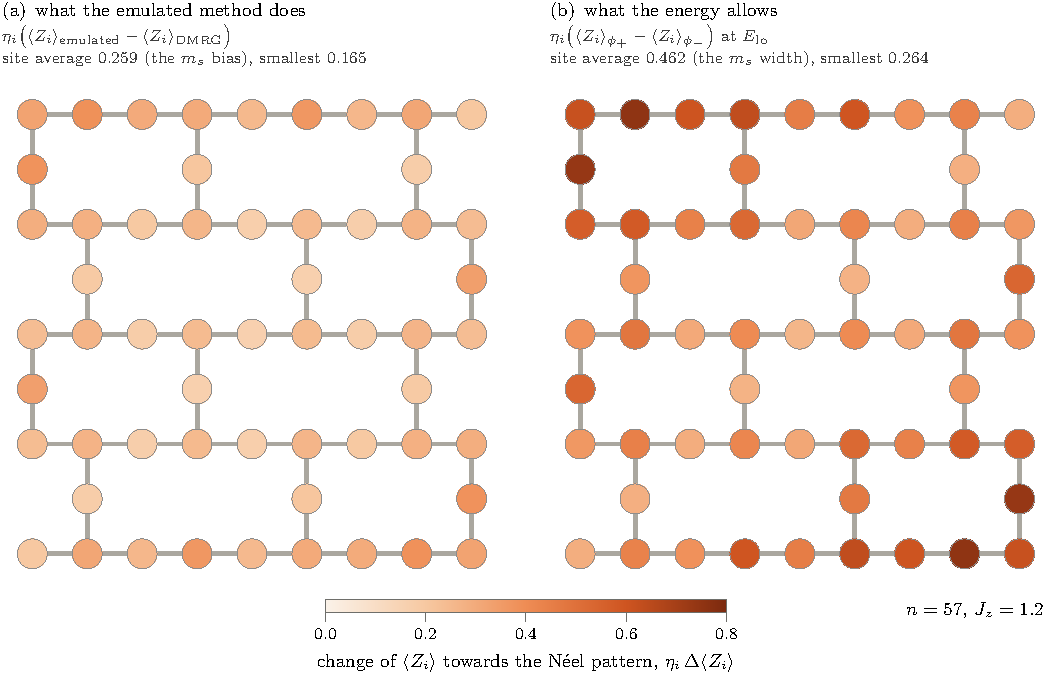
\includegraphics[width=\textwidth]{figS_lattice_pgf}%
\caption{\label{fig:lattice57}Site by site at $\Jz=1.2$, $n=57$, on the dataset's heavy-hex lattice (circles: sites; % src: file:phase3/full_runs/method/RESULTS.md; file:phase3/full_runs/method/laptop_post/results_tables.md; def:phase3/full_runs/method/DECLARATION.md
lines: bonds; the usual drawing of the coupling map, every bond of unit length). (a) What the emulated method class
does: the signed excess of order $\eta_i(\langle Z_i\rangle_{\rm emulated}-\langle Z_i\rangle_{\rm DMRG})$ of the
primary variant at its own energy, positive at every site; its site average is the $\ms$ bias. (b) What the energy
allows: $\eta_i(\langle Z_i\rangle_{\phi_+}-\langle Z_i\rangle_{\phi_-})$ between the two explicit $\ms$ witnesses
of the window at $E_{\rm lo}$ (the floor that the map built from the figures assumed at this coupling; the public
energy error per site there is $0.0198$, Sec.~\ref{sm:public}), whose site average is the $\ms$ width. Same colour scale; % src: rdp:sizes.57.P5.rows[Jz=1.2].de (0.019759)
$\eta_i=+1$ on the majority colour. The emulated state lies at a higher energy than the witnesses ($\de=0.043$ % src: file:phase3/full_runs/method/RESULTS.md; file:phase3/full_runs/method/laptop_post/results_tables.md; def:phase3/full_runs/method/DECLARATION.md
against $0.0096$), so the panels compare patterns, not positions in one window; the position of the emulated states in % src: file:phase3/full_runs/method/RESULTS.md; file:phase3/full_runs/method/laptop_post/results_tables.md; def:phase3/full_runs/method/DECLARATION.md; derived: 0.8 x 0.012 = 0.0096 (witness-side window at the conditional floor)
their window is in ancillary Table~A7. Source: deposited emulated and reference labels, and the stored % src: file:phase3/full_runs/method/RESULTS.md; file:phase3/full_runs/method/laptop_post/results_tables.md; def:phase3/full_runs/method/DECLARATION.md
witness states of the map with their mixture weights.}
\end{figure}


\needspace{0.7\textheight} % src: file:phase3/full_runs/method/RESULTS.md; file:phase3/full_runs/method/laptop_post/results_tables.md; def:phase3/full_runs/method/DECLARATION.md
\subsection{Mechanism}
\def\SMcap{The pipeline step by step at fixed $(n,\Jz)$. Columns go from perfect samples of the DMRG ground state
(cut to the primary subspace dimension: the ground state projected on the sampled configurations, then Rayleigh--Ritz
in them) to the emulated Krylov pipeline with increasing noise. The three blocks give, for the same rows and columns,
the signed bias $\Delta\ms$, the subspace dimension $D$ and the energy ratio $r$ (``---'': not applicable or not
run). Read along a row of the top block: Rayleigh--Ritz in the perfect samples already reproduces the bias of the
full pipeline; noise adds to it.}\def\SMlab{tab:meth_steps}
% generated by figures/make_sm_tables.py from phase3/full_runs/method/laptop_post/results_tables.md Table 2 -- do not edit
{\footnotesize\setlength{\tabcolsep}{5pt}\renewcommand{\arraystretch}{1.3}
\needspace{454pt}
\begin{longtable}{lccccccc}
\caption{\SMcap}\label{\SMlab}\\
\toprule
 & \multicolumn{2}{c}{perfect ground-state samples} & \multicolumn{5}{c}{emulated Krylov pipeline} \\ \cmidrule(lr){2-3}\cmidrule(l){4-8}
$n$, $J_z$ & \begin{tabular}[b]{@{}c@{}}support\\only\end{tabular} & \begin{tabular}[b]{@{}c@{}}+ Rayleigh--\\Ritz\end{tabular} & \begin{tabular}[b]{@{}c@{}}no\\noise\end{tabular} & \begin{tabular}[b]{@{}c@{}}1\,\% flips +\\recovery\\(primary)\end{tabular} & \begin{tabular}[b]{@{}c@{}}device-like\\noise, post-\\selected\end{tabular} & \begin{tabular}[b]{@{}c@{}}device-like\\noise +\\recovery\end{tabular} & \begin{tabular}[b]{@{}c@{}}noise matched\\to raw energy\\($n=57$)\end{tabular} \\
\midrule
\multicolumn{8}{@{}l}{\textbf{signed bias $\Delta m_s$}}\\
57, 1.2 & $+$0.175 & $+$0.258 & $+$0.253 & $+$0.259 & $+$0.328 & $+$0.323 & $+$0.316 \\
57, 1.6 & $+$0.070 & $+$0.127 & $+$0.134 & $+$0.139 & $+$0.201 & $+$0.196 & --- \\
57, 2.5 & $+$0.009 & $+$0.027 & $+$0.033 & $+$0.036 & $+$0.079 & $+$0.077 & $+$0.073 \\
57, 4.0 & \phantom{$+$}0.000\rlap{$^{e}$} & \phantom{$+$}0.000\rlap{$^{e}$} & $+$0.004 & $+$0.005 & $+$0.025 & $+$0.023 & $+$0.021 \\
115, 1.2 & $+$0.277 & $+$0.317 & $+$0.297 & $+$0.301 & $+$0.323 & $+$0.322 & --- \\
115, 1.6 & $+$0.146 & $+$0.181 & $+$0.178 & $+$0.181 & $+$0.201 & $+$0.201 & --- \\
115, 2.5 & $+$0.037 & $+$0.061 & $+$0.065 & $+$0.067 & $+$0.084 & $+$0.084 & --- \\
\multicolumn{8}{@{}l}{\textbf{subspace dimension $D$}}\\
57, 1.2 & --- & --- & \hfill216\,155 & \hfill336\,818 & \hfill81\,416 & \hfill975\,896 & \hfill919\,518 \\
57, 1.6 & --- & --- & \hfill253\,802 & \hfill375\,441 & \hfill81\,762 & \hfill976\,316 & --- \\
57, 2.5 & --- & --- & \hfill165\,800 & \hfill291\,117 & \hfill81\,696 & \hfill975\,689 & \hfill920\,028 \\
57, 4.0 & --- & --- & \hfill95\,807 & \hfill214\,674 & \hfill81\,939 & \hfill975\,918 & \hfill920\,398 \\
115, 1.2 & --- & --- & \hfill240\,031 & \hfill472\,401 & \hfill82\,291 & \hfill986\,974 & --- \\
115, 1.6 & --- & --- & \hfill247\,167 & \hfill479\,203 & \hfill81\,562 & \hfill986\,668 & --- \\
115, 2.5 & --- & --- & \hfill191\,771 & \hfill431\,473 & \hfill82\,203 & \hfill986\,601 & --- \\
\multicolumn{8}{@{}l}{\textbf{energy ratio $r=(E-E_0)/(E_1-E_0)$}}\\
57, 1.2 & --- & --- & 14.1\phantom{000} & 15.2\phantom{000} & 32.4\phantom{00} & 31.3\phantom{0} & 29.5\phantom{00} \\
57, 1.6 & --- & --- & \phantom{0}2.64\phantom{00} & \phantom{0}2.93\phantom{00} & \phantom{0}7.81\phantom{0} & \phantom{0}7.44 & --- \\
57, 2.5 & --- & --- & \phantom{0}0.331\phantom{0} & \phantom{0}0.395\phantom{0} & \phantom{0}1.84\phantom{0} & \phantom{0}1.74 & \phantom{0}1.59\phantom{0} \\
57, 4.0 & --- & --- & \phantom{0}0.0303 & \phantom{0}0.0415 & \phantom{0}0.429 & \phantom{0}0.4\phantom{0} & \phantom{0}0.351 \\
115, 1.2 & --- & --- & 43\phantom{.0000} & 44.6\phantom{000} & 61.9\phantom{00} & 61.7\phantom{0} & --- \\
115, 1.6 & --- & --- & 11.8\phantom{000} & 12.4\phantom{000} & 19.2\phantom{00} & 18.6\phantom{0} & --- \\
115, 2.5 & --- & --- & \phantom{0}2.44\phantom{00} & \phantom{0}2.6\phantom{000} & \phantom{0}5.1\phantom{00} & \phantom{0}5\phantom{.00} & --- \\
\bottomrule
\end{longtable}
\vspace{-6pt}\noindent{\scriptsize $^{e}$\,extrapolated.}\par\medskip
}


\noindent Perfect sampling with nested subspaces (ancillary Table~A6): for every $(n,\Jz)$ the multiplicity-weighted % src: file:phase3/full_runs/method/RESULTS.md; file:phase3/full_runs/method/laptop_post/results_tables.md; def:phase3/full_runs/method/DECLARATION.md
sample mean is unbiased, while the Rayleigh--Ritz vector and the projected ground state stay biased as $D$ grows.

\noindent At $n=57$, $\Jz=1.2$, raising the subspace from $10^6$ to $3.16\times10^6$ configurations lowers the % src: file:phase3/full_runs/method/RESULTS.md (10^6); meth:decisions.D3_n57.D_max (3158635)
bias only from $0.239$ to $0.218$: % src: meth:decisions.D3_n57.dm_s_at_1e6 (0.2388); meth:decisions.D3_n57.dm_s_at_Dmax (0.2177)
it falls roughly as $D^{-0.074}$; a power-law extrapolation to $3\%$ of $\ms$ % src: meth:decisions.D3_n57.powerlaw.exponent; file:phase3/full_runs/method/RESULTS.md (3 %)
would need $D\approx6\times10^{20}$ configurations, which we quote only to show that the bias does not vanish at any reachable % src: meth:decisions.D3_n57.powerlaw.D_for_3pct_extrapolated
size. At $n=115$, $\Jz=1.2$ the $10^5$ most probable configurations already carry all the captured weight, and the % src: file:phase3/full_runs/method/RESULTS.md; file:phase3/full_runs/method/laptop_post/results_tables.md; def:phase3/full_runs/method/DECLARATION.md
remaining $7\times10^5$ sampled strings change neither the energy nor the labels. % src: file:phase3/full_runs/method/RESULTS.md; file:phase3/full_runs/method/laptop_post/results_tables.md; def:phase3/full_runs/method/DECLARATION.md

\begin{figure}[h]
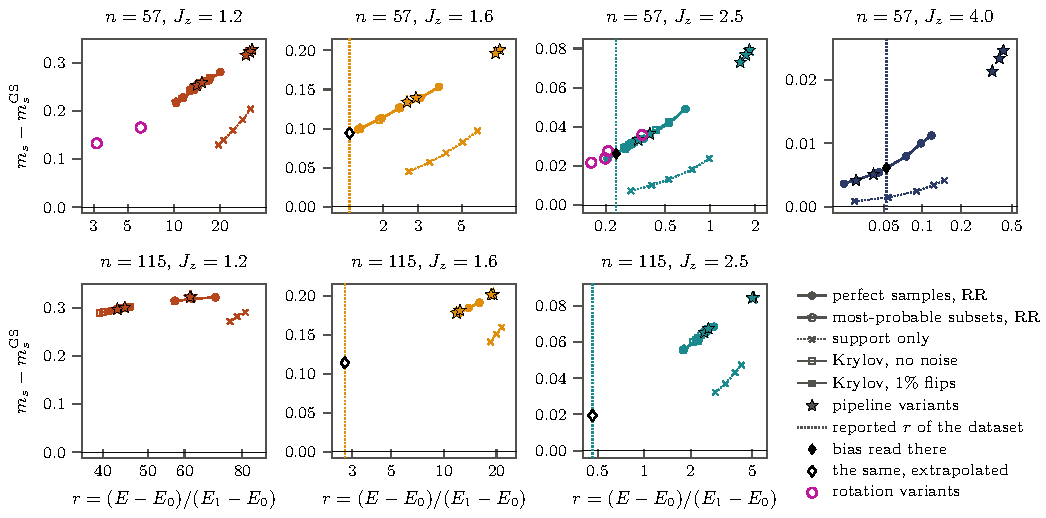
\includegraphics[width=\textwidth]{figS1_bias_vs_ratio_pgf}%
\caption{Signed $\ms$ bias against the energy ratio for every emulated family at every $(n,\Jz)$ with a perfect-sampler
scan; markers as in Fig.~\ref{figS:mechanism}, colours $\Jz$. Dotted: the dataset's reported ratio (its Fig.~2,
digitized; none at $\Jz=1.2$); diamonds: the bias read there (open: extrapolated beyond the sampled ratios); magenta circles: % src: file:phase3/full_runs/method/RESULTS.md; file:phase3/full_runs/method/laptop_post/results_tables.md; def:phase3/full_runs/method/DECLARATION.md
labels of the physical state after the two rotation variants of Sec.~\ref{sm:bo}, which the text of
Ref.~\cite{jaderberg2026} does not describe (the one with $R_Y$ on the control qubit is the block of its public
code~\cite{jaderberg2026data}).
Source: deposited method outputs.}
\end{figure}

\subsection{The basis-optimization step}
\label{sm:bo}
Implemented as we read the dataset paper's Methods and Supp.\ Secs.~II.3--II.3.1: $H'=UHU^\dagger$, % src: file:phase3/full_runs/method/RESULTS.md; file:phase3/full_runs/method/laptop_post/results_tables.md; def:phase3/full_runs/method/DECLARATION.md
$C(\theta)=\alpha^\dagger H'_B\alpha$ with the subspace vector $\alpha$ fixed; $U$ one layer of
CNOT$(c\to t)\cdot R_Y^{(t)}(\theta)\cdot$CNOT$(c\to t)=e^{-i\theta Z_cY_t/2}$ over all 64 edges in the three colour % src: file:phase3/full_runs/method/RESULTS.md; file:phase3/full_runs/method/laptop_post/results_tables.md; def:phase3/full_runs/method/DECLARATION.md
sub-layers, with the rotation on the target qubit as the text and its circuit diagram place it; exact Pauli
propagation; analytic gradient; re-diagonalization of $H'_B(\theta^*)$ in the same subspace.
Unspecified choices, all run: orientation (control on the minority or the majority colour), per-gate angles or one
shared angle (721-point scan plus refinement), initialization, and the stated local/global procedure. \emph{Why there is % src: file:phase3/full_runs/method/RESULTS.md; file:phase3/full_runs/method/laptop_post/results_tables.md; def:phase3/full_runs/method/DECLARATION.md
no gain:} the block flips one spin, so splitting $H=H_c+H_a$ into terms that commute or anticommute with $Z_cY_t$,
$\Pi UHU^\dagger\Pi=\Pi H\Pi-(1-\cos\theta)\Pi H_a\Pi$ inside the sector; $C(\theta)$ is even in $\theta$ and, on % src: file:phase3/full_runs/method/RESULTS.md; file:phase3/full_runs/method/laptop_post/results_tables.md; def:phase3/full_runs/method/DECLARATION.md
antiferromagnetically correlated subspaces, $\theta=0$ is a minimum. We therefore tried two variants that the text does not describe, $R_Y$ % src: file:phase3/full_runs/method/RESULTS.md; file:phase3/full_runs/method/laptop_post/results_tables.md; def:phase3/full_runs/method/DECLARATION.md
on the control wire and a number-conserving Givens block, both declared and run on 2026-10-30, before we knew the % src: def:phase3/full_runs/method/DECLARATION.md (2026-10-30); file:phase3/full_runs/method/RESULTS.md (2026-10-30)
public repository; both reproduce the reported gain (Tables~\ref{tab:meth_bo_energy} and \ref{tab:meth_bo_labels}).
The former, like the block as described, does not conserve the particle number, so with it the physical states
$U^\dagger\psi'$ leave the sector; only the Givens variant keeps them in it. The public
record~\cite{jaderberg2026data} settles two points that this paragraph had to leave open. The block: the code
of the repository, which we read as text and did not run, places on each edge a CNOT, $R_Y(\theta)$ on the control
qubit and the same CNOT, with one angle per edge (function \texttt{build\_variational\_circuit} of
\texttt{qaml/skqd/basis\_optimise.py}, which the script that computes the published labels calls), and its gradient
routine names the generator, $Y$ on the control and $X$ on the target. This is the former of our two variants,
$e^{-i\theta Y_cX_t/2}$, and not the block drawn in the paper, $e^{-i\theta Z_cY_t/2}$. The same code evaluates each
label as the expectation value of the rotated operator in the re-diagonalized vector, that is, in the physical state
$U^\dagger\psi'$ (file \texttt{qaml/observables/modified\_basis.py}). We did not compare the order and orientation of
the CNOTs or the optimizer with ours. The optimized angles are not in the repository, and that this code produced the
published files is the authors' statement, which the files cannot prove. The sector: the final states are not in the
sector. The sum of the published site magnetizations lies below the sector value at all $50$ couplings of both % src: rdam:B_sector.57.n_negative (50); rdam:B_sector.115.n_negative (50)
sizes, by $0.0003$--$0.2342$ at $n=57$ and $0.0026$--$0.4353$ at $n=115$ (Sec.~\ref{sm:public}), as a rotation that % src: rdam:B_sector.57.max (-0.00037); rdam:B_sector.57.min (-0.23420); rdam:B_sector.115.max (-0.00268); rdam:B_sector.115.min (-0.43520); derived: ranges rounded outward
does not conserve the particle number can produce and a number-conserving one cannot. The record also holds the
energy before and after the step: it lowers the energy error per site by factors of $2.8$--$8.9$ at $n=57$ (median % src: rdp:post_hoc.per_size.57.de_first_over_de_real.min (2.80); rdp:post_hoc.per_size.57.de_first_over_de_real.max (8.93)
$6.7$) and $6.6$--$175$ at $n=115$ (median $30$). The map of the main text therefore uses the window of energy and % src: rdp:post_hoc.per_size.57.de_first_over_de_real.median (6.67); rdp:post_hoc.per_size.115.de_first_over_de_real.min (6.59); rdp:post_hoc.per_size.115.de_first_over_de_real.max (175.4); rdp:post_hoc.per_size.115.de_first_over_de_real.median (29.6)
mean magnetization, not the sector window, for the public labels (Sec.~\ref{sm:public}).

\def\SMcap{Basis optimization at $n=57$: energy. Each row is one variant of the rotation layer: the block (the stated % src: file:phase3/full_runs/method/RESULTS.md; file:phase3/full_runs/method/laptop_post/results_tables.md; def:phase3/full_runs/method/DECLARATION.md
CNOT--$R_Y$--CNOT with the rotation on the target qubit, or one of two variants that the text does not describe: $R_Y$
on the control qubit, the block of the public code, and a number-conserving Givens block), whether its angles are per gate, shared, or set by the stated
local/global procedure, and which colour of the bipartition carries the control. $f$: fraction of the energy error
$E-E_0$ removed; $r$: energy ratio before and after; $\theta_{\rm rms}$: root-mean-square optimized angle. Read down a % src: file:phase3/full_runs/method/RESULTS.md; file:phase3/full_runs/method/laptop_post/results_tables.md; def:phase3/full_runs/method/DECLARATION.md
block: the stated block never lowers the energy ($f=0$, $\theta\approx0$); both other variants do.}\def\SMlab{tab:meth_bo_energy} % src: file:phase3/full_runs/method/RESULTS.md; file:phase3/full_runs/method/laptop_post/results_tables.md; def:phase3/full_runs/method/DECLARATION.md
% generated by figures/make_sm_tables.py from phase3/full_runs/method/laptop_post/results_tables.md Table 4 -- do not edit
{\footnotesize\setlength{\tabcolsep}{5pt}\renewcommand{\arraystretch}{1.3}
\needspace{516pt}
\begin{longtable}{llcccc}
\caption{\SMcap}\label{\SMlab}\\
\toprule
Block & angles, control colour & $f$ & $r$ before & $r$ after & $\theta_{\rm rms}$ \\
\midrule
\multicolumn{6}{@{}l}{\textbf{$J_z=1.2$, primary subspace}}\\
stated (CNOT--$R_Y$--CNOT) & per gate, minority & 0.000 & 15.2\phantom{00} & 15.2\phantom{00} & $2.1\times10^{-7}$ \\
stated (CNOT--$R_Y$--CNOT) & per gate, majority & 0.000 & 15.2\phantom{00} & 15.2\phantom{00} & $5.3\times10^{-7}$ \\
stated (CNOT--$R_Y$--CNOT) & one shared, minority & 0.000 & 15.2\phantom{00} & 15.2\phantom{00} & $1.3\times10^{-10}$ \\
stated (CNOT--$R_Y$--CNOT) & one shared, majority & 0.000 & 15.2\phantom{00} & 15.2\phantom{00} & $1.3\times10^{-10}$ \\
stated (CNOT--$R_Y$--CNOT) & stated procedure, minority & 0.000 & 15.2\phantom{00} & 15.2\phantom{00} & 0 \\
stated (CNOT--$R_Y$--CNOT) & stated procedure, majority & 0.000 & 15.2\phantom{00} & 15.2\phantom{00} & 0 \\
$R_Y$ on the control wire & per gate, minority & 0.601 & 15.2\phantom{00} & \phantom{0}6.07\phantom{0} & $1.8\times10^{-1}$ \\
$R_Y$ on the control wire & per gate, majority & 0.601 & 15.2\phantom{00} & \phantom{0}6.07\phantom{0} & $1.8\times10^{-1}$ \\
Givens (number-conserving) & per gate & 0.795 & 15.2\phantom{00} & \phantom{0}3.13\phantom{0} & $1.2\times10^{-1}$ \\
\multicolumn{6}{@{}l}{\textbf{$J_z=2.5$, device-like noise + recovery subspace}}\\
stated (CNOT--$R_Y$--CNOT) & per gate, minority & 0.000 & \phantom{0}1.74\phantom{0} & \phantom{0}1.74\phantom{0} & $4.4\times10^{-7}$ \\
stated (CNOT--$R_Y$--CNOT) & per gate, majority & 0.000 & \phantom{0}1.74\phantom{0} & \phantom{0}1.74\phantom{0} & $1.6\times10^{-6}$ \\
stated (CNOT--$R_Y$--CNOT) & one shared, minority & 0.000 & \phantom{0}1.74\phantom{0} & \phantom{0}1.74\phantom{0} & $1.3\times10^{-10}$ \\
stated (CNOT--$R_Y$--CNOT) & one shared, majority & 0.000 & \phantom{0}1.74\phantom{0} & \phantom{0}1.74\phantom{0} & $1.3\times10^{-10}$ \\
stated (CNOT--$R_Y$--CNOT) & stated procedure, minority & 0.000 & \phantom{0}1.74\phantom{0} & \phantom{0}1.74\phantom{0} & 0 \\
stated (CNOT--$R_Y$--CNOT) & stated procedure, majority & 0.000 & \phantom{0}1.74\phantom{0} & \phantom{0}1.74\phantom{0} & 0 \\
$R_Y$ on the control wire & per gate, minority & 0.798 & \phantom{0}1.74\phantom{0} & \phantom{0}0.352 & $1.5\times10^{-1}$ \\
$R_Y$ on the control wire & per gate, majority & 0.798 & \phantom{0}1.74\phantom{0} & \phantom{0}0.352 & $1.5\times10^{-1}$ \\
Givens (number-conserving) & per gate & 0.881 & \phantom{0}1.74\phantom{0} & \phantom{0}0.208 & $4.0\times10^{-1}$ \\
\multicolumn{6}{@{}l}{\textbf{$J_z=2.5$, primary subspace}}\\
stated (CNOT--$R_Y$--CNOT) & per gate, minority & 0.000 & \phantom{0}0.395 & \phantom{0}0.395 & $1.6\times10^{-7}$ \\
stated (CNOT--$R_Y$--CNOT) & per gate, majority & 0.000 & \phantom{0}0.395 & \phantom{0}0.395 & $7.7\times10^{-7}$ \\
stated (CNOT--$R_Y$--CNOT) & one shared, minority & 0.000 & \phantom{0}0.395 & \phantom{0}0.395 & $1.3\times10^{-10}$ \\
stated (CNOT--$R_Y$--CNOT) & one shared, majority & 0.000 & \phantom{0}0.395 & \phantom{0}0.395 & $1.3\times10^{-10}$ \\
stated (CNOT--$R_Y$--CNOT) & stated procedure, minority & 0.000 & \phantom{0}0.395 & \phantom{0}0.395 & 0 \\
stated (CNOT--$R_Y$--CNOT) & stated procedure, majority & 0.000 & \phantom{0}0.395 & \phantom{0}0.395 & 0 \\
$R_Y$ on the control wire & per gate, minority & 0.498 & \phantom{0}0.395 & \phantom{0}0.199 & $5.0\times10^{-2}$ \\
$R_Y$ on the control wire & per gate, majority & 0.498 & \phantom{0}0.395 & \phantom{0}0.199 & $5.0\times10^{-2}$ \\
Givens (number-conserving) & per gate & 0.595 & \phantom{0}0.395 & \phantom{0}0.16\phantom{0} & $2.9\times10^{-2}$ \\
\bottomrule
\end{longtable}
}


\def\SMcap{Basis optimization at $n=57$: labels, for the two variants that lower the energy (the stated block % src: file:phase3/full_runs/method/RESULTS.md; file:phase3/full_runs/method/laptop_post/results_tables.md; def:phase3/full_runs/method/DECLARATION.md
leaves the state unchanged). $\Delta\ms$ before and after the rotation, read off the rotated vector $\psi'$ directly or
from the physical state $U^\dagger\psi'$, and the energy of $\psi'$ under the original $H$ (above $E_0$, units of the % src: file:phase3/full_runs/method/RESULTS.md; file:phase3/full_runs/method/laptop_post/results_tables.md; def:phase3/full_runs/method/DECLARATION.md
exchange coupling). Read along a row: labels read off $\psi'$ are more over-ordered than before, and $\psi'$ itself has
a high energy; the physical state has a smaller bias, on the same bias-versus-energy curve as all other
states.}\def\SMlab{tab:meth_bo_labels}
% generated by figures/make_sm_tables.py from phase3/full_runs/method/laptop_post/results_tables.md Table 4 -- do not edit
{\footnotesize\setlength{\tabcolsep}{5pt}\renewcommand{\arraystretch}{1.3}
\needspace{298pt}
\begin{longtable}{llcccc}
\caption{\SMcap}\label{\SMlab}\\
\toprule
 & & & \multicolumn{2}{c}{$\Delta m_s$ after} & \\ \cmidrule(lr){4-5}
Block & angles, control colour & $\Delta m_s$ before & read off $\psi'$ & physical $U^\dagger\psi'$ & $E(\psi')-E_0$ under $H$ \\
\midrule
\multicolumn{6}{@{}l}{\textbf{$J_z=1.2$, primary subspace}}\\
$R_Y$ on the control wire & per gate, minority & $+$0.259 & $+$0.287 & $+$0.166 & 2.783 \\
$R_Y$ on the control wire & per gate, majority & $+$0.259 & $+$0.287 & $+$0.166 & 2.783 \\
Givens (number-conserving) & per gate & $+$0.259 & $+$0.295 & $+$0.133 & 3.021 \\
\multicolumn{6}{@{}l}{\textbf{$J_z=2.5$, device-like noise + recovery subspace}}\\
$R_Y$ on the control wire & per gate, minority & $+$0.077 & $+$0.090 & $+$0.036 & 2.170 \\
$R_Y$ on the control wire & per gate, majority & $+$0.077 & $+$0.090 & $+$0.036 & 2.170 \\
Givens (number-conserving) & per gate & $+$0.077 & $+$0.091 & $+$0.028 & 2.233 \\
\multicolumn{6}{@{}l}{\textbf{$J_z=2.5$, primary subspace}}\\
$R_Y$ on the control wire & per gate, minority & $+$0.036 & $+$0.049 & $+$0.024 & 0.487 \\
$R_Y$ on the control wire & per gate, majority & $+$0.036 & $+$0.049 & $+$0.024 & 0.487 \\
Givens (number-conserving) & per gate & $+$0.036 & $+$0.051 & $+$0.022 & 0.510 \\
\bottomrule
\end{longtable}
}


\noindent If labels are those of the physical state $U^\dagger\psi'$, they fall on the bias-versus-energy curve of all
other states. If they are read off $\psi'$ directly, they are more over-ordered than before the rotation and $\psi'$
has an energy under $H$ far above the reported one. The dataset paper does not say which; the code of the public
record computes them in the physical state (above), and the public labels agree with that: at their published energies their bias is $0.80$--$1.05$ of the curve of the first stage at $n=57$ and $0.60$--$0.82$ at % src: rdp:sizes.57.P5.all.ratio_range_deciding (0.8029, 1.0455); rdp:sizes.115.P5.all.ratio_range_deciding (0.6087, 0.8122); derived: ranges rounded outward
$n=115$ at the couplings where it matters (Sec.~\ref{sm:publiccurve}), on or below the relation of all emulated
states, as labels of the physical state are in our two variants and as labels read off $\psi'$ are not.

\needspace{0.4\textheight} % src: file:phase3/full_runs/method/RESULTS.md; file:phase3/full_runs/method/laptop_post/results_tables.md; def:phase3/full_runs/method/DECLARATION.md
\subsection{Reading at the dataset's energy and position in the window}
The two routes of this subsection were our estimates of the bias of the dataset's labels before those labels were
known to be public; they are kept as they were written. The labels now give the bias itself (Sec.~\ref{sm:publictests}),
and a comparison made afterwards, which no declaration covers, sets the estimates next to it. At $n=57$ the measured
bias of $\ms$ is $+0.077$, $+0.022$ and $+0.006$ at $\Jz=1.6$, $2.5$ and $4.0$, against $+0.094$, $+0.026$ and % src: rdp:sizes.57.P5.rows[Jz=1.6].Delta (0.0771); rdp:sizes.57.P5.rows[Jz=2.5].Delta (0.0221); rdp:sizes.57.P5.rows[Jz=4.0].Delta (0.0063); meth:bias_at_ibm_energy.57_1.6.dm_s (0.0942); meth:bias_at_ibm_energy.57_2.5.dm_s (0.0262)
$+0.006$ for Route~1 and $+0.080$, $+0.020$ and $+0.005$ for Route~2; at $\Jz=1.2$, where only Route~2 applies, it % src: meth:bias_at_ibm_energy.57_4.0.dm_s (0.0061); meth:dZ_matched.57_1.6.dm_s (0.0797); meth:dZ_matched.57_2.5.dm_s (0.0195); meth:dZ_matched.57_4.0.dm_s (0.0048)
is $+0.157$ ($n=57$) and $+0.144$ ($n=115$) against $+0.159$ and $+0.146$. The sign that Route~2 had to assume is the % src: rdp:sizes.57.P5.rows[Jz=1.2].Delta (0.1574); rdp:sizes.115.P5.rows[Jz=1.2].Delta (0.1441); meth:dZ_matched.57_1.2.dm_s (0.1589); meth:dZ_matched.115_1.2.dm_s (0.1458); derived: Route 2 is a name
measured one (Sec.~\ref{sm:publictests}). Its close agreement in size is expected rather than a test: Route~2 is the % src: derived: Route 2 is a name
dataset paper's own unsigned error turned into a signed mean with the slope of the emulated states, and what it took
from the emulation that the measurement could have contradicted is the sign.


\def\SMcap{Route 1: the bias read at the dataset's reported energy ratio $r$ (its Fig.~2), by interpolation in % src: file:phase3/full_runs/method/RESULTS.md; file:phase3/full_runs/method/laptop_post/results_tables.md; def:phase3/full_runs/method/DECLARATION.md
$\log r$ along the perfect-sampler bias-versus-energy curve, with its low--high range and whether $r$ lies inside the
computed curve (\emph{interpolated}) or beyond it (\emph{extrapolated}). The last two columns check the route: the
$\langle Z_i\rangle$ error $\Delta Z$ it predicts at that $r$ against the one the dataset paper reports (its Supp.\
Fig.~11). Read along a row: the route over-predicts $\Delta Z$, so it gives an upper estimate.}\def\SMlab{tab:meth_at_energy} % src: file:phase3/full_runs/method/RESULTS.md; file:phase3/full_runs/method/laptop_post/results_tables.md; def:phase3/full_runs/method/DECLARATION.md
% generated by figures/make_sm_tables.py from phase3/full_runs/method/laptop_post/results_tables.md Table 5 -- do not edit
{\footnotesize\setlength{\tabcolsep}{5pt}\renewcommand{\arraystretch}{1.3}
\needspace{233pt}
\begin{longtable}{lccccccc}
\caption{\SMcap}\label{\SMlab}\\
\toprule
 & & \multicolumn{3}{c}{$\Delta m_s$ at that $r$} & & \multicolumn{2}{c}{$\Delta Z$ (\%)} \\ \cmidrule(lr){3-5}\cmidrule(l){7-8}
$J_z$ & dataset's $r$ & estimate & low & high & reading & predicted & dataset \\
\midrule
\multicolumn{8}{@{}l}{\textbf{$n=57$}}\\
1.6 & 1.348\phantom{0} & $+$0.094 & $+$0.092 & $+$0.097 & \textit{extrapolated} & 12.5 & 10.6 \\
2.5 & 0.235\phantom{0} & $+$0.026 & $+$0.025 & $+$0.027 & \textit{interpolated} & \phantom{0}2.9 & \phantom{0}2.2 \\
4.0 & 0.0523 & $+$0.006 & $+$0.006 & $+$0.006 & \textit{interpolated} & \phantom{0}0.6 & \phantom{0}0.5 \\
\multicolumn{8}{@{}l}{\textbf{$n=115$}}\\
1.6 & 2.716\phantom{0} & $+$0.114 & $+$0.112 & $+$0.116 & \textit{extrapolated} & 15.0 & 10.0 \\
2.5 & 0.464\phantom{0} & $+$0.019 & $+$0.018 & $+$0.021 & \textit{extrapolated} & \phantom{0}2.2 & \phantom{0}2.0 \\
\bottomrule
\end{longtable}
}


\def\SMcap{Route 2: the bias from the dataset paper's own unsigned $\langle Z_i\rangle$ error, $\Delta\ms=k\,\Delta % src: file:phase3/full_runs/method/RESULTS.md; file:phase3/full_runs/method/laptop_post/results_tables.md; def:phase3/full_runs/method/DECLARATION.md
Z$, with the slope $k$ (value and low--high range) of all emulated states at that point and \emph{with their sign},
which is assumed, not measured, for the dataset; every emulated state
over-orders, and $k$ is constant to $\pm0.5\,\%$. Also given: the reference $\ms$ and the energy ratio at which the % src: file:phase3/full_runs/method/RESULTS.md; file:phase3/full_runs/method/laptop_post/results_tables.md; def:phase3/full_runs/method/DECLARATION.md
perfect-sampler curve would reach this bias (``---'': no curve at that point). This is the only route at the
out-of-distribution points ($\Jz\le1.4$).}\def\SMlab{tab:meth_dz_matched} % src: file:phase3/full_runs/method/RESULTS.md; file:phase3/full_runs/method/laptop_post/results_tables.md; def:phase3/full_runs/method/DECLARATION.md
% generated by figures/make_sm_tables.py from phase3/full_runs/method/laptop_post/results_tables.md Table 6 -- do not edit
{\footnotesize\setlength{\tabcolsep}{5pt}\renewcommand{\arraystretch}{1.3}
\needspace{350pt}
\begin{longtable}{lccccccc}
\caption{\SMcap}\label{\SMlab}\\
\toprule
 & & \multicolumn{3}{c}{slope $k=\Delta m_s/\Delta Z$} & & & \\ \cmidrule(lr){3-5}
$J_z$ & dataset's $\Delta Z$ (\%) & value & low & high & $\Delta m_s$ estimate & $m_s$ reference & implied $r$ \\
\midrule
\multicolumn{8}{@{}l}{\textbf{$n=57$}}\\
1.1 & 31.6 & 0.00562 & 0.00561 & 0.00563 & $+$0.178 & 0.595 & --- \\
1.2 & 26.0 & 0.00611 & 0.00610 & 0.00615 & $+$0.159 & 0.640 & 5.05\phantom{00}\rlap{$^{e}$} \\
1.3 & 21.8 & 0.00654 & 0.00653 & 0.00654 & $+$0.142 & 0.680 & --- \\
1.4 & 16.9 & 0.00691 & 0.00690 & 0.00691 & $+$0.117 & 0.714 & --- \\
1.6 & 10.6 & 0.00752 & 0.00750 & 0.00754 & $+$0.080 & 0.770 & 0.948\phantom{0}\rlap{$^{e}$} \\
2.5 & \phantom{0}2.2 & 0.00888 & 0.00887 & 0.00889 & $+$0.020 & 0.897 & 0.158\phantom{0}\rlap{$^{e}$} \\
4.0 & \phantom{0}0.5 & 0.00955 & 0.00954 & 0.00956 & $+$0.005 & 0.959 & 0.0378 \\
\multicolumn{8}{@{}l}{\textbf{$n=115$}}\\
1.1 & 29.8 & 0.00587 & 0.00587 & 0.00587 & $+$0.175 & 0.620 & --- \\
1.2 & 23.0 & 0.00634 & 0.00633 & 0.00635 & $+$0.146 & 0.662 & 0.791\phantom{0}\rlap{$^{e}$} \\
1.3 & 18.5 & 0.00674 & 0.00674 & 0.00675 & $+$0.125 & 0.700 & --- \\
1.4 & 14.8 & 0.00710 & 0.00709 & 0.00710 & $+$0.105 & 0.732 & --- \\
1.6 & 10.0 & 0.00767 & 0.00766 & 0.00767 & $+$0.077 & 0.785 & 0.328\phantom{0}\rlap{$^{e}$} \\
2.5 & \phantom{0}2.0 & 0.00895 & 0.00894 & 0.00897 & $+$0.018 & 0.903 & 0.154\phantom{0}\rlap{$^{e}$} \\
4.0 & \phantom{0}0.4 & 0.00957 & 0.00957 & 0.00958 & $+$0.004 & 0.961 & --- \\
\bottomrule
\end{longtable}
\vspace{-6pt}\noindent{\scriptsize $^{e}$\,extrapolated along the perfect-sampler curve.}\par\medskip
}


\noindent Where the emulated states sit in their window (ancillary Table~A7): every state lies on the ``$+$'' side % src: file:phase3/full_runs/method/RESULTS.md; file:phase3/full_runs/method/laptop_post/results_tables.md; def:phase3/full_runs/method/DECLARATION.md
($f_+>0$, with $f_+$ the fraction of the greatest excess of order the energy permits), most of them in its upper half. % src: file:phase3/full_runs/method/RESULTS.md; file:phase3/full_runs/method/laptop_post/results_tables.md; def:phase3/full_runs/method/DECLARATION.md

\noindent Uncertainties: digitization of the dataset paper's Supp.\ Fig.~11 ($\pm1$ point) gives $\pm0.006$ in % src: file:phase3/full_runs/method/RESULTS.md; file:phase3/full_runs/method/laptop_post/results_tables.md; def:phase3/full_runs/method/DECLARATION.md
$\Delta\ms$ at $\Jz\le1.4$; at $n=57$ the perfect-sampler curve of Route~1 over-predicts the published $\Delta Z$ by % src: file:phase3/full_runs/method/RESULTS.md; file:phase3/full_runs/method/laptop_post/results_tables.md; def:phase3/full_runs/method/DECLARATION.md
about a fifth to a third at $\Jz=1.6$, $2.5$, $4.0$ ($12.5$, $2.9$, $0.6\%$ against $10.6$, $2.2$, $0.5\%$; % src: file:phase3/full_runs/method/laptop_post/results_tables.md (12.5, 2.9, 0.6; 10.6, 2.2, 0.5)
Table~\ref{tab:meth_at_energy}), so the two routes bracket the estimate. The cubic fitted to all emulated $n=57$ states
in Sec.~V of the main text, a different curve, gives $18$, $39$ and $29\%$ at the same points. These are estimates for the method % src: blw:published.rows (18.39, 39.37, 29.49)
class at the dataset's published quality; the statements about the labels themselves are the measurements of
Sec.~\ref{sm:publictests}.

\subsection{Readings of the dataset paper's figures}
We read: its Fig.~2 (left) and Supp.\ Fig.~9 for the energy ratios; its Fig.~4 (left) for the gap; its Supp.\ % src: file:phase3/full_runs/method/RESULTS.md; file:phase3/full_runs/method/laptop_post/results_tables.md; def:phase3/full_runs/method/DECLARATION.md
Fig.~11 for the unsigned mean relative errors of $\langle Z_i\rangle$, $C_{zz}$ and loops against its DMRG reference, % src: file:phase3/full_runs/method/RESULTS.md; file:phase3/full_runs/method/laptop_post/results_tables.md; def:phase3/full_runs/method/DECLARATION.md
including the OOD points; and the colour scale of its Fig.~4 (right; $\Jz=1.1$, $n=115$), whose 41 labelled sites % src: file:phase3/full_runs/method/RESULTS.md; file:phase3/full_runs/method/laptop_post/results_tables.md; def:phase3/full_runs/method/DECLARATION.md
were inverted against the figure's own colour bar and compared with our DMRG reference at the same point (bond
dimension $200$, not fully converged). All 41 sites have larger $|\langle Z_i\rangle|$ than the reference; we use this % src: file:phase3/full_runs/method/RESULTS.md; file:phase3/full_runs/method/laptop_post/results_tables.md; def:phase3/full_runs/method/DECLARATION.md
only as a sign. \emph{This is a reading of a colour scale in a published figure against an unconverged reference,
not a measurement and not a claim about the published labels; it appears in this Supplement only.} The public
labels at that point now give the measurement: all $115$ sites are more ordered than the authors' reference % src: rdp:sizes.115.P1_P3.sites.F_per_coupling.1.1 (1.0); rdp:sizes.115.P1_P3.sites.n_items (115)
(Sec.~\ref{sm:publictests}). The in-sector and unique-string counts quoted in its Methods were used for the noise calibration.

\section{Our device data}
\label{sm:qpu}

\emph{Run.} The raw stage of the method class (Krylov sampling, random-flip recovery or post-selection, Rayleigh--Ritz
in the sampled configurations; no basis optimization) was run at $n=57$ on \texttt{ibm\_kingston} (an IBM Heron r2 % src: file:phase3/full_runs/qpu/RESULTS.md; def:phase3/full_runs/qpu/DECLARATION.md; file:phase3/full_runs/qpu/analysis/TABLES.md
processor) through the IBM Quantum free plan, on 2026-10-31, with one calibration for both jobs. The Krylov circuits % src: file:phase3/full_runs/qpu/RESULTS.md; def:phase3/full_runs/qpu/DECLARATION.md; file:phase3/full_runs/qpu/analysis/TABLES.md
use the published time steps. The dataset's heavy-hex graph does not embed natively in the device's coupling map;
a routed layout moves four boundary sites (25, 30, 31, 36). Circuit $k$ then has $224k$ CZ gates and CZ depth $14k+1$: % src: file:phase3/full_runs/qpu/RESULTS.md; def:phase3/full_runs/qpu/DECLARATION.md; file:phase3/full_runs/qpu/analysis/TABLES.md
at $k=10$, 2240 and 141 against 1920 and 91 for a native embedding of the same circuit, i.e.\ $17\%$ more two-qubit % src: file:phase3/full_runs/qpu/RESULTS.md; def:phase3/full_runs/qpu/DECLARATION.md; file:phase3/full_runs/qpu/analysis/TABLES.md
gates and $55\%$ more depth. Shots: $10^5$ per circuit at $\Jz=1.2$, and 23\,000 per circuit at $1.6$ and $4.0$ % src: file:phase3/full_runs/qpu/RESULTS.md; def:phase3/full_runs/qpu/DECLARATION.md; file:phase3/full_runs/qpu/analysis/TABLES.md
(fewer than the declared 32\,000, to keep the second job within its time cap). Processor time: 421\,s. % src: file:phase3/full_runs/qpu/RESULTS.md; def:phase3/full_runs/qpu/DECLARATION.md; file:phase3/full_runs/qpu/analysis/TABLES.md
A third job, the declared run at $\Jz=6.0$, ran on the same device on 2026-11-10 ($119$\,s, a new calibration); it is % src: file:phase3/full_runs/final_tests/RESULTS.md (6.0; 2026-11-10; 119.0 s)
reported in Sec.~\ref{sec:declared}, not in Table~\ref{tab:qpu}.

\emph{Checks.} Before the Krylov circuits, each job measured the N\'eel state and an asymmetric product state; the
declared pass condition (every site at least $90\%$ in agreement with the expected bit, and the majority correct) % src: file:phase3/full_runs/qpu/RESULTS.md; def:phase3/full_runs/qpu/DECLARATION.md; file:phase3/full_runs/qpu/analysis/TABLES.md
held in both jobs (smallest site agreement $0.919$--$0.940$, mean $0.985$--$0.987$); an incorrect bit order would put whole % src: file:phase3/full_runs/qpu/RESULTS.md; def:phase3/full_runs/qpu/DECLARATION.md; file:phase3/full_runs/qpu/analysis/TABLES.md
groups of sites near zero agreement. The compiled $k=1$ circuits were checked against the logical ones on a simulator % src: file:phase3/full_runs/qpu/RESULTS.md; def:phase3/full_runs/qpu/DECLARATION.md; file:phase3/full_runs/qpu/analysis/TABLES.md
before submission (greatest difference of $\langle Z_i\rangle$: $3.0\times10^{-11}$). The noiseless control simulates the % src: file:phase3/full_runs/qpu/RESULTS.md; def:phase3/full_runs/qpu/DECLARATION.md; file:phase3/full_runs/qpu/analysis/TABLES.md; file:phase3/full_runs/qpu/RESULTS.md (3.0e-11)
identical circuits with matrix-product states (bond dimension $\le256$, discarded weight $\le2.5\times10^{-7}$) and % src: file:phase3/full_runs/qpu/RESULTS.md; def:phase3/full_runs/qpu/DECLARATION.md; file:phase3/full_runs/qpu/analysis/TABLES.md
applies the same post-processing; at $\Jz=1.2$ it coincides with the exact-evolution emulation to the digits shown in % src: file:phase3/full_runs/qpu/RESULTS.md; def:phase3/full_runs/qpu/DECLARATION.md; file:phase3/full_runs/qpu/analysis/TABLES.md
Table~\ref{tab:qpu}, so the Trotter error does not affect the labels at this budget.

\def\SMcap{Our device data at $n=57$, with the noiseless control of the identical circuits and the emulation of % src: file:phase3/full_runs/qpu/RESULTS.md; def:phase3/full_runs/qpu/DECLARATION.md; file:phase3/full_runs/qpu/analysis/TABLES.md
Sec.~\ref{sm:emu} for comparison. $D$: subspace dimension; $r=(E-E_0)/(E_1-E_0)$; $\Delta\ms$: signed bias against the % src: file:phase3/full_runs/qpu/RESULTS.md; def:phase3/full_runs/qpu/DECLARATION.md; file:phase3/full_runs/qpu/analysis/TABLES.md
DMRG reference; smallest site excess: $\min_i\eta_i(\langle Z_i\rangle-\langle Z_i\rangle_{\rm DMRG})$, positive in every
row; $\Delta Z$, $\Delta C_{zz}$: mean relative errors of the site labels and of the nearest-neighbour correlations.
In every row all 57 sites are more ordered than the reference.}\def\SMlab{tab:qpu} % src: file:phase3/full_runs/qpu/RESULTS.md; def:phase3/full_runs/qpu/DECLARATION.md; file:phase3/full_runs/qpu/analysis/TABLES.md
% generated by figures/make_sm_new.py from phase3/full_runs/qpu/analysis/analysis.json (points.*.device/control/emulation_1e6_shots) -- do not edit
{\footnotesize\setlength{\tabcolsep}{5pt}\renewcommand{\arraystretch}{1.3}
\needspace{334pt}
\begin{longtable}{@{}lccccccc@{}}
\caption{\SMcap}\label{\SMlab}\\
\toprule
source & shots/circuit & $D$ & $r$ & $\Delta m_s$ & \begin{tabular}[b]{@{}c@{}}smallest\\site excess\end{tabular} & $\Delta Z$ (\%) & $\Delta C_{zz}$ (\%) \\
\midrule
\multicolumn{8}{@{}l}{\textbf{$J_z=1.2$}}\\
device, recovery & 100\,000 & 935\,497 & 28.6 & $+0.310$ & $+0.202$ & 50.5 & 72.0 \\
device, post-selection & 100\,000 & 133\,914 & 29.9 & $+0.315$ & $+0.210$ & 51.4 & 73.6 \\
noiseless control & 100\,000 & 215\,576 & 14.1 & $+0.253$ & $+0.160$ & 41.4 & 54.4 \\
emulation, device-like noise ($10^6$ shots) & --- & --- & 31.3 & $+0.323$ & --- & --- & --- \\
emulation, noiseless ($10^6$ shots) & --- & --- & 14.1 & $+0.253$ & --- & --- & --- \\
\multicolumn{8}{@{}l}{\textbf{$J_z=1.6$}}\\
device, recovery & 23\,000 & 217\,393 & 7.58 & $+0.196$ & $+0.122$ & 26.0 & 38.3 \\
noiseless control & 23\,000 & 72\,540 & 3.71 & $+0.153$ & $+0.094$ & 20.4 & 28.2 \\
emulation, device-like noise ($10^6$ shots) & --- & --- & 7.44 & $+0.196$ & --- & --- & --- \\
emulation, noiseless ($10^6$ shots) & --- & --- & 2.64 & $+0.134$ & --- & --- & --- \\
\multicolumn{8}{@{}l}{\textbf{$J_z=4.0$}}\\
device, recovery & 23\,000 & 218\,647 & 0.437 & $+0.024$ & $+0.013$ & 2.51 & 3.79 \\
noiseless control & 23\,000 & 32\,395 & 0.0723 & $+0.008$ & $+0.005$ & 0.820 & 1.20 \\
emulation, device-like noise ($10^6$ shots) & --- & --- & 0.400 & $+0.023$ & --- & --- & --- \\
emulation, noiseless ($10^6$ shots) & --- & --- & 0.0303 & $+0.004$ & --- & --- & --- \\
\bottomrule
\end{longtable}
}


\emph{Reading.} The over-ordering is present at every site of our device data at all three couplings. The noiseless
control produces most of it ($+0.253$ of $+0.310$ at $\Jz=1.2$); the device noise adds $+0.057$, $+0.043$ and $+0.016$ at % src: file:phase3/full_runs/qpu/RESULTS.md; def:phase3/full_runs/qpu/DECLARATION.md; file:phase3/full_runs/qpu/analysis/TABLES.md
$\Jz=1.2$, $1.6$ and $4.0$, close to the $+0.070$ that the independent bit-flip model of the emulation predicted at % src: file:phase3/full_runs/qpu/RESULTS.md; def:phase3/full_runs/qpu/DECLARATION.md; file:phase3/full_runs/qpu/analysis/TABLES.md
$1.2$. Our raw-stage energy ratios are $1.10$ and $1.19$ times the raw-stage ratios read from the dataset paper's figures % src: file:phase3/full_runs/qpu/RESULTS.md; def:phase3/full_runs/qpu/DECLARATION.md; file:phase3/full_runs/qpu/analysis/TABLES.md
at $\Jz=1.6$ and $4.0$. On the map, our device energies lie $1151$, $288$ and $2.7$ times above the error at which $\ms$ % src: file:phase3/full_runs/qpu/RESULTS.md; def:phase3/full_runs/qpu/DECLARATION.md; file:phase3/full_runs/qpu/analysis/TABLES.md
would be certified at $1.2$, $1.6$ and $4.0$: none of these three device points is certified. At $6.0$ the energy error % src: file:phase3/full_runs/qpu/RESULTS.md; def:phase3/full_runs/qpu/DECLARATION.md; file:phase3/full_runs/qpu/analysis/TABLES.md; file:phase3/full_runs/final_tests/RESULTS.md (6.0)
of the declared job is $0.32$ times that threshold, and its interval is proved below $\tau$, at a coupling where a % src: ft3:C3.rec.eps (0.2278); map:row(57,6.0,m_s).eps_tau_out (0.72026); derived: 0.2278 / 0.72026 = 0.316
classical energy gives a narrower one (Sec.~\ref{sec:declared}). ``Certified'' here refers to the sector window:
the device states are in the sector, and these thresholds come from DMRG chains, not from any published energy.
The device energies at those three couplings lie beyond the range of % (structural)
the ``$+$'' chains, so their position inside the window is only bounded and we claim none. Not checked: run-to-run
variation (a single run per point; two jobs for the three couplings) and a native embedding, which these devices do not allow for this graph.
The public labels of the dataset, which come from the full method, show the same sign at every site, with two
exceptions in one state (Sec.~\ref{sm:publictests}).

\section{What does not help at this scale}
\label{sm:nohelp}

\begin{proposition}[Conjugate labels and several couplings]
Write $H(x)=A+xB$ ($A=\frac14\sum(XX+YY)$, $B=\frac14\sum ZZ$, $x=\Jz$) and $E_0(y)$ its concave sector ground energy. % src: file:phase3/design/R2_constructive_half.md
For $E>E_0(x)$, $\max\{\langle B\rangle_\rho:\langle H(x)\rangle_\rho\le E\}=\inf_{y<x}[E-E_0(y)]/(x-y)$ and the % src: file:phase3/design/R2_constructive_half.md
minimum is $\sup_{y>x}[E_0(y)-E]/(y-x)$, attained by mixtures of ground states of $H(y)$. Hence energies reported at % src: file:phase3/design/R2_constructive_half.md
other couplings, which are upper bounds on $E_0(y)$, cannot narrow the interval for the truth at $x$: with exact % src: file:phase3/design/R2_constructive_half.md
references the multi-coupling bracket equals the single-point information limit.
\end{proposition}
\noindent\emph{Proof.} $H(x)-\lambda B=H(x-\lambda)$ and Lemma~A. $\square$ In exact checks at $n=12$ the generic % src: file:phase3/design/R2_constructive_half.md
field limit of $\Czz$, the Legendre bracket and the curve of neighbouring ground states agree to $10^{-5}$. At the % src: file:phase3/design/R2_constructive_half.md
dataset scale the $\Czz$ widths of the map are these brackets (the $\Czz$ field is a shift of $\Jz$).

\begin{remark}[Side information about the generated state]
Data on the generated state $\psi$ (its labels, energy variance, separately measured bond energies) constrain the
ground state through a variational inequality, i.e.\ an upper bound on $E_0$, or through a fidelity bound from the % src: file:phase3/design/R2_constructive_half.md
energy variance and a gap (Temple-type~\cite{temple1928}), together with a-priori ground-state properties (sector, symmetry, eigen-equation). We know
of no other bridge; the next paragraph evaluates the fidelity route.
\end{remark}

\emph{Energy variance.} A reported variance $V_{\rm dev}$ of the generated state excludes a witness only if the
witness has a larger variance. In exact checks at $n=12$ the extremal $\ms$ witnesses have $V/\epsilon^2=7$--$12$, % src: file:phase3/design/R2_constructive_half.md
$32$--$46$ and $164$--$195$ at $\Jz=1.6$, $2.5$, $4.0$, while truncated-diagonalization states of the same energy have % src: file:phase3/design/R2_constructive_half.md
$23$--$25$, $95$--$104$ and $397$--$421$: two to three times more, so no witness is excluded. The fidelity route % src: file:phase3/design/R2_constructive_half.md
(of Temple type~\cite{temple1928}) needs $V$ smaller by factors of $80$--$5000$ at $n=12$, and $V$ is extensive while the gap % src: file:phase3/design/R2_constructive_half.md
is not. The eigenstate second-moment constraint helps only when $E_0$ is known to better than the gap minus $2\epsilon$. % src: file:phase3/design/R2_constructive_half.md

\emph{Symmetry.} The dataset's graphs have only two automorphisms (one rotation; 56 of 57 and 114 of 115 sites in % src: file:phase3/design/R2_constructive_half.md
orbits of size two). In exact checks at $n=12$ restricting the window to symmetric states leaves $\ms$ and $\Czz$ % src: file:phase3/design/R2_constructive_half.md
unchanged to $10^{-14}$ and narrows local labels by factors $0.68$--$0.77$, i.e.\ by $23$ to $32\%$. % src: file:phase3/design/R2_constructive_half.md; derived: 1 - 0.77 = 23 % and 1 - 0.68 = 32 %
Stoquasticity adds nothing for diagonal labels, because every diagonal-field witness is stoquastic too.

\section{Learning with certified labels}
\label{sm:learn}
\makeatletter\providecommand{\LTclearhead}{\global\setbox\LT@head\box\voidb@x}\makeatother

\subsection{Proofs of Proposition 2 of the main text, its floor, and a remark on energy-only procedures} % (structural: proposition number)
\label{sm:prop2proofs}

\emph{Setting.} Inputs $x$ (here the coupling vector of a Hamiltonian $H(x)$) are exchangeable; the true label
$y^*(x)$ is the ground-state value, a function of $x$. The generator returns a label $y(x)$ and an energy $E(x)$; the
window theory returns an interval $I(x)=[\ell(x),h(x)]$, of width $w(x)$, that contains $y^*(x)$ and the label of
every state with energy at most $E(x)$, in particular $y(x)$ (Lemma~A of the main text; for the public labels, the
exact interval of Sec.~\ref{sm:public}, which uses the published energy and mean magnetization; at $n=20$ the intervals hold over all states, % src: file:phase3/full_runs/learning/RESULTS.md (n = 20)
since the benchmark's SU(2) symmetry makes the sector restriction unnecessary). A learner is \emph{linear in its % (structural: SU(2))
labels} if $f(x)=\sum_{i=1}^Na_i(x)\,y_i$, with coefficients that depend on the training inputs, on $x$ and on fixed
hyperparameters but not on the labels; kernel ridge regression and ridge regression on fixed features are of this
form, with $a(x)=(K+\lambda\mathbb 1)^{-1}k(x)$ for kernel ridge, and so is the kernel estimator analysed in
Ref.~\cite{huang2022}. The estimator of Ref.~\cite{lewis2024} is not, because it uses an $\ell_1$ penalty; it
becomes linear in its labels when that penalty is replaced by a ridge, as in model M2 below. $f^*$ denotes the same
learner trained on the true labels.

\emph{(a) Label-induced error.} $f(x)-f^*(x)=\sum_ia_i(x)(y_i-y_i^*)$, and $y_i,y_i^*\in I_i$ give
$|y_i-y_i^*|\le h_i-\ell_i$, so $|f(x)-f^*(x)|\le\sum_i|a_i(x)|(h_i-\ell_i)=W(x)$. No probability enters, so the bound
holds at every $x$, also outside the training distribution. It is attained: the image of the box $\prod_i I_i$ under
$y\mapsto f(x)$ is exactly $[f_{\rm lo}(x),f_{\rm hi}(x)]$ with $f_{\rm hi}-f_{\rm lo}=W(x)$, and it contains
$f^*(x)$ and $f(x)$. With $w_i\le\max_jw_j$, $W(x)\le\|a(x)\|_1\max_jw_j$; with the widths of Theorems~1 and~2 of % (structural: theorem numbers)
the main text ($w\simeq2\sqrt{2\bar\chi\de}$ for an average, independent of $n$; $w\simeq2\sqrt{2\chi_in\de}$ for a
local label up to $N^*$), the label-induced error of a linear learner inherits the certification law, multiplied by
its label sensitivity $\|a(x)\|_1$. $\square$

\emph{(b) Coverage of the truth.} Let $S(x,y)\ge0$ be any score computed from the trained learner (for instance
$|f(x)-y|$), $s_j=\max_{y\in I_j}S(x_j,y)$ for the $m$ calibration inputs, and $q$ the
$k$-th smallest $s_j$, $k=\lceil(m+1)(1-\alpha)\rceil$ ($q=+\infty$ if $k>m$). For a new input exchangeable with the
calibration inputs, the set $C(x)=\{y:S(x,y)\le q\}$ satisfies
$P(y^*(x)\in C(x))\ge1-\alpha$; the probability is over the calibration inputs and the new input jointly. Proof: with the learner trained on separate data, the true-label scores
$s_j^*=S(x_j,y^*(x_j))$ and $s^*=S(x,y^*(x))$ are exchangeable, so $P(s^*\le q^*)\ge1-\alpha$ for their conformal
quantile $q^*$ (the standard split-conformal argument~\cite{angelopoulos2021}). Since $y^*(x_j)\in I_j$,
$s_j\ge s_j^*$ for every $j$, hence every order statistic, and $q$, is at least the corresponding one of the
true-label scores: $q\ge q^*$, and $P(s^*\le q)\ge P(s^*\le q^*)\ge1-\alpha$. Nothing is assumed about how $y(x_j)$
relates to $y^*(x_j)$ beyond both lying in $I_j$; the generator's error may be one-signed, adversarial and correlated
with $x$. The price is bounded: for $S=|f-y|$, $s_j\le s_j^*+(h_j-\ell_j)$, so $q\le q^*+\max_jw_j$. We call the
resulting intervals energy-calibrated. The energy-calibrated constructions of the test (abbreviations as in the
deposited files) are CSC ($S=|f-y|$), CNC ($S=|f-y|/\sigma(x)$, $\sigma$ an ensemble spread) and CB
($S=\max(0,\,y-f_{\rm hi}(x),\,f_{\rm lo}(x)-y)$, i.e.\ the band of (a) widened by $q$); for CNC the statement is
approximate, because the normalization used in the test includes the median spread of the calibration sample, so its
score is not computed from the trained learner alone. The construction is the pessimistic score of
Ref.~\cite{javanmardi2023} for set-valued labels, there for classification, applied to intervals; the proof of its
validity (Theorem~1 there) is the argument above. Ref.~\cite{cauchois2022} shows that covering the true label for % (structural: theorem number of the cited work)
every law consistent with set-valued labels forces sets about as large as the label sets (its Theorem~1 and % (structural: theorem number of the cited work)
Corollary~2.3; Remark below) and therefore targets a weaker coverage; the width cost measured in this section is % (structural: corollary number of the cited work)
that price. Ref.~\cite{einbinder2022} shows that standard calibration stays valid for the true label under noise
that only adds dispersion, and corrects for noise of known total-variation size by changing the level, a different
mechanism. What the physics adds is the interval itself, computed from the label's energy. The standard score
$|f(x_j)-y_j|$ gives the same guarantee for $y(x)$ only. $\square$

\emph{(c) Selective error.} If $y^*(x)\in C(x)$ and $|C(x)|\le\tau$, the midpoint $c(x)$ satisfies
$|c(x)-y^*(x)|\le|C(x)|/2\le\tau/2$. Hence $\{|C(x)|\le\tau\}\cap\{|c(x)-y^*(x)|>\tau/2\}\subseteq\{y^*(x)\notin % (structural: tau/2)
C(x)\}$, whose probability is at most $\alpha$, and the error rate among answers,
$P(|c-y^*|>\tau/2\mid\text{answered})$, is at most $\alpha/P(\text{answered})$. The rule ``answer iff
$W(x)\le\tau$'' has instead the deterministic guarantee of (a): every answer is within $\tau$ of $f^*(x)$; it says
nothing about $|f^*(x)-y^*(x)|$, the learner's own error. $\square$

\emph{(d) Floor.} For any real number $f$ and any interval $[\ell,h]$,
$\max_{y\in[\ell,h]}|f-y|=\max(|f-\ell|,|f-h|)\ge(h-\ell)/2$, with equality if and only if $f$ is the midpoint.
So $s_j\ge w_j/2$ for every $j$, and an order statistic of numbers that dominate others dominates the same order
statistic of the others: $q=s_{(k)}\ge w_{(k)}/2$. If every $f(x_j)$ is a midpoint, $s_j=w_j/2$ and $q=w_{(k)}/2$.
Nothing is assumed about the learner or about the labels it was trained on. $\square$

Part (d) is the constant-width case of the following statement, which also says what holds for other scores.

\begin{proposition}[A floor for the energy-calibrated intervals]
\label{prop:floor}
In the setting of (b), let $w_{(1)}\le\dots\le w_{(m)}$ be the widths of the calibration intervals in increasing
order and $k=\lceil(m+1)(1-\alpha)\rceil$.
(i) For the score $|f(x)-y|$ and every learner, that is, for any real numbers $f(x_1),\dots,f(x_m)$,
$2q\ge w_{(k)}$ ($q=+\infty$ if $k>m$), with equality if $f(x_j)$ is the midpoint of $I_j$ for all $j$.
(ii) With scores normalized by a positive function $\sigma$, $s_j=\max_{y\in I_j}|f(x_j)-y|/\sigma(x_j)$ and
interval $f(x)\pm q\,\sigma(x)$, the width at $x$ is at least $\sigma(x)\,[w_j/\sigma(x_j)]_{(k)}$.
(iii) For any score $S\ge0$: if the new input has an energy interval $I(x)$ of width $w(x)$ and the pair
$(x,I(x))$ is exchangeable with the calibration pairs, then $P(I(x)\subseteq C(x))\ge1-\alpha$; when $C(x)$
is an interval, it is at least $w(x)$ wide with that probability.
(iv) Consequently rule (c) with the intervals of (i) can answer only if at least $k$ of the $m$ calibration labels
have energy intervals no wider than the tolerance at the query; and with any score whose set $C(x)$ is an
interval, the event that it answers at an input whose own energy interval is wider than its tolerance has
probability at most $\alpha$.
(v) The condition of (iv) on the calibration labels is special to the constant-width score: with $\sigma(x)$ proportional to $w(x)$ and
midpoint predictions every score equals the same constant and the interval of (ii) at $x$ is exactly $I(x)$,
whatever the widths of the calibration intervals.
\end{proposition}

\emph{Proof.} (i) is (d). (ii) The same with $s_j\ge w_j/(2\sigma(x_j))$.
(iii) Let $s(x)=\max_{y\in I(x)}S(x,y)$. With the score fixed and the pairs exchangeable, the numbers
$s_1,\dots,s_m,s(x)$ are exchangeable, so $P(s(x)\le s_{(k)})\ge k/(m+1)\ge1-\alpha$; and $s(x)\le q$ is the
event $I(x)\subseteq C(x)$.
(iv) With the score of (i) the rule answers only if $2q\le\tau$, which by (i) requires $w_{(k)}\le\tau$. If
$C(x)$ is an interval no wider than $\tau$ and $w(x)>\tau$, then $I(x)\not\subseteq C(x)$, an event of
probability at most $\alpha$ by (iii).
(v) With $\sigma(x_j)=a\,w_j$ and midpoint predictions, $s_j=1/(2a)$ for all $j$, so $q=1/(2a)$ and
$f(x)\pm q\,\sigma(x)=f(x)\pm w(x)/2$. $\square$

Parts (i) and (ii) hold for any numbers in place of $f(x_j)$, hence also for the leave-one-out predictions of the
jackknife calibration of Secs.~\ref{sm:realistic} and~\ref{sm:publiclearn}, to which the coverage statement (iii)
does not apply. The hypothesis of (iii) is exchangeability of the pairs (input, energy interval), because the
interval depends on the generator's energy, which is not a function of the input alone.
\emph{What the floor gives, and its limits.} With the constant-width score, a guarantee at the tolerance needs
calibration labels of which at least $k$ of $m$ have energy intervals no wider than it. This is a condition on the
calibration labels, not on the training labels: (b) holds for any learner trained on separate data, and a wide
interval for one model and one score is a statement about that model and score, not an impossibility for others.
For other scores the floor is the query's own energy interval, in the sense of (iii). Neither floor says anything
about a learner's accuracy. Values: Sec.~\ref{sm:realistic} for the emulated labels and Sec.~\ref{sm:publiclearn}
for the public labels, where the constructive side is tested.

\begin{remark}[Energy-only procedures; after Theorem~1 and Corollary~2.3 of Ref.~\cite{cauchois2022}] % (structural: theorem and corollary numbers of the cited work)
\label{rem:anyproc}
The generator returns at each input $x$ a state with label $y(x)$ and energy $E(x)$; $I(x)=[\ell(x),h(x)]$, of width
$w(x)$, is the set of labels of the states of its window, an interval because the window is convex, and every point
of it is the label of a state of the window. The data are $\mathcal D=\{(X_j,y(X_j),E(X_j))\}_{j\le m}$ and $X$ is
a new input. A \emph{reference} is a measurable choice $x\mapsto t(x)\in I(x)$; the true label $y^*$ is one. A
procedure is a jointly measurable map $(\mathcal D,X,\zeta,\omega)\mapsto C(X)\subseteq\mathbb R$, where $\zeta$
stands for any information that is the same for all references (the Hamiltonians, the intervals, a label and an
energy at the query) and $\omega$ is independent randomness. Call a procedure \emph{energy-only at level
$1-\alpha$} if $P(t(X)\in C(X))\ge1-\alpha$ for every reference $t$. This is the strong distribution-free coverage
of Ref.~\cite{cauchois2022} (Definition~2.2 there) with the energy interval as the weak label set, required for % (structural: definition number of the cited work)
deterministic label maps. Proposition~2(b) of the main text is of this kind, with any score, when the pairs are % (structural: proposition number)
exchangeable [Proposition~\ref{prop:floor}(iii)], and so is every certificate of Sec.~II of the main text. Then,
for the new input:
(a) $C(X)$ contains both ends of $I(X)$ with probability at least $1-2\alpha$; if $C(X)$ is an interval, it
contains $I(X)$ and is at least $w(X)$ wide with that probability, so that for a rule which answers only when the
interval is at most $\tau$ long the event that it answers at an input whose own energy interval is wider than $\tau$
has probability at most $2\alpha$.
(b) If $w>0$ for all inputs, the expected fraction of $I(X)$ covered by $C(X)$ is at least $1-\alpha$; if $w\ge L$
for all inputs, the expected length of $C(X)$ is at least $(1-\alpha)L$, which is Corollary~2.3 of % (structural: corollary number of the cited work)
Ref.~\cite{cauchois2022}. The constants $1-2\alpha$, $1-\alpha$ and $2\alpha$ are attained.
\end{remark}

\emph{Proof.} The joint law of $(\mathcal D,X,C(X))$ does not depend on the reference, which enters only the event
whose probability is bounded. (a) Apply the definition to $t=h$ and to $t=\ell$:
$P(h(X)\notin C(X)\ \text{or}\ \ell(X)\notin C(X))\le2\alpha$. An interval that contains $\ell(X)$ and $h(X)$
contains $I(X)$, and an interval of length at most $\tau$ cannot contain both ends when $w(X)>\tau$. (b) For
$u\in[0,1]$ let $t_u=\ell+uw$, a reference. Then $P(t_u(X)\in C(X))\ge1-\alpha$ for each $u$, and integrating
over $u$ (Fubini) gives
\[
\mathbb E\!\left[\frac{\mathrm{Leb}(C(X)\cap I(X))}{w(X)}\right]=\int_0^1P\big(t_u(X)\in C(X)\big)\,du\ \ge\ 1-\alpha ; % (formula)
\]
if $w\ge L$, $\mathbb E\,\mathrm{Leb}(C(X))\ge L\,\mathbb E[\mathrm{Leb}(C\cap I)/w]\ge(1-\alpha)L$.
Attainment: the procedure that returns $I(X)$ with probability $1-\alpha$ and the empty set otherwise is
energy-only and covers a fraction exactly $1-\alpha$ on average; the procedure that returns $I(X)$ with
probability $1-2\alpha$, and otherwise $I(X)$ without a piece at its upper or at its lower end (probability
$\alpha$ each), is energy-only when the two pieces are disjoint and contains both ends with probability exactly
$1-2\alpha$; with pieces of length $w-\tau$, for $\tau<w\le2\tau$, the answering rule of (a) answers with
probability exactly $2\alpha$. $\square$

For Proposition~2(b) itself, (a) holds with $1-\alpha$ in place of $1-2\alpha$ [Proposition~\ref{prop:floor}(iii)], % (structural: proposition number)
because its score is the greatest over the window. The statement on the answering rule is for intervals: for sets
that are not intervals it fails if the size of $C(X)$ is its Lebesgue measure, since $I(X)$ without an arc of
length $\alpha\,w(X)$ at a uniformly random cyclic position covers every reference with probability $1-\alpha$ and
always has measure $(1-\alpha)w(X)$ (Ref.~\cite{cauchois2022} makes the same point with the procedure that
includes every label independently with probability $1-\alpha$).

\emph{What the remark gives.} Certifying a learner's prediction from the energies alone is not easier than
certifying a label from its energy at the same input: the query's own energy interval is a floor for every
learner, score and calibration scheme, so pooling labels across inputs or assuming a smooth label map does not
help, and an interval-valued learner-side rule answers where the label filter would not with probability at most
$2\alpha$. A procedure that solves $H(x)$, or uses more than the energies, is not bound by it.

\emph{What is not shown, and where a stronger statement fails.} (i) The hypothesis is coverage of every reference,
not only of the true label. With coverage of the true label alone the conclusion is false: for a fixed and known
family $H(x)$ the true label is one function of $x$, and the procedure that outputs it has zero width. The
remark is thus a statement about a mode of justification, of the same kind as the statement of Sec.~II of the main
text for certificates; it follows from its hypothesis in two lines, and what it records is that pooling over inputs
does not help.
(ii) Corollary~2(b) of the main text does not supply a two-point argument for the true label. It compares two generators with the % (structural: corollary number)
same energies whose labels differ, and so the two situations do not have the same data. Two situations with the
same data and different true labels require two Hamiltonians. They exist: if $\rho$ has label $y$ and energy $E$
under $H$, then under $H_\nu=H-\nu(O-ny)$ it has the same label and the same energy for every $\nu$, while the
true label is that of the ground state of $H-\nu O$. With $\rho$ the ground state of $H-\nu_0O$, the true label
for $\nu=\nu_0$ is the upper end of the window of $H$ at $E$, and the lower end is the true label for
$\nu=-\nu_0'$, where $\nu_0'$ is the field at which the ground state of $H+\nu_0'O$ has energy $E$; $\nu_0'=\nu_0$
when a symmetry maps $O$ to $-O$ (ring of $8$ sites, $\Jz=2.5$, $\nu_0=0.05$: identical $(y,E)=(0.8468,-5.7751)$, % src: file:paper/reviews/R10_2026-11-12/theory/lemmas/attack_F2_out.txt (ring of 8 sites, Jz = 2.5; 0.05; 0.84684; 5.775106)
true labels $\pm0.8468$), and not otherwise ($10$-site piece of the heavy-hex lattice, $\Jz=2.5$, $\nu_0=0.05$: % src: file:paper/reviews/R10_2026-11-12/theory/lemmas/attack_F2_out.txt (0.84684; 0.05); file:paper/reviews/R10_2026-11-12/scratch/break-lemmas/break_F_out.txt (n = 10, Jz = 2.5)
$\nu_0'=0.0402$). A procedure that sees only $(x,y,E)$ and covers the true label for both fields must then contain % src: file:paper/reviews/R10_2026-11-12/scratch/break-lemmas/break_F_out.txt (0.0402)
both ends with probability $1-2\alpha$. But the energy intervals computed with the true Hamiltonian differ
between the two situations (a point for $\nu=+\nu_0$, where the generator is exact; a wide interval for
$\nu=-\nu_0'$), so a procedure that knows the Hamiltonian tells them apart. That floor is therefore a statement
about an unknown conjugate field of the label, a hypothesis this paper does not make.
(iii) For references restricted to labels of ground states of the deformed local families, (a) holds as stated
when the ends of $I(x)$ are attained at finite fields; (b) uses all points of the interval and needs the
intermediate value property of the label along the deformed family, which holds when that family has no level
crossing.

\emph{Checks} (scripts of an internal review, not part of the declared analyses). On the eight couplings with a map row
of the emulated-label study at $n=57$, with the held-out coupling drawn uniformly, fifteen energy-only procedures % (sizes)
(Proposition~2(b) with constant and with width-normalized scores for six learners, the window itself, and the two % (structural: proposition number)
procedures of the attainment argument) were enumerated exactly against $203$ references, with no violation of (a) % src: file:paper/reviews/R10_2026-11-12/theory/lemmas/attack_F2_out.txt (203 references)
or (b); standard conformal intervals calibrated on the labels are not energy-only (some reference is never
covered). In a synthetic exchangeable setting ($m=19$, $\alpha=0.1$) the interval of Proposition~2(b) contains the % src: file:paper/reviews/R10_2026-11-12/theory/lemmas/attack_F2_out.txt (alpha = 0.1, m = 19)
query's interval with frequency $0.899$ and covers a fraction $0.988$ of it, against the bounds $0.80$ and $0.90$. % src: file:paper/reviews/R10_2026-11-12/theory/lemmas/attack_F2_out.txt (0.8992; 0.9885; bound 0.80; bound 0.90)

\subsection{Protocol}

\emph{Data.} The $100$ instances at $n=20$ ($4\times5$ open lattice) of Ref.~\cite{huang2022}, official repository, % src: file:phase3/full_runs/learning/RESULTS.md (100 n = 20 instances)
read as data only, solved by exact diagonalization: residuals at most $3.6\times10^{-11}$, our ground energy at or % src: file:phase3/full_runs/learning/RESULTS.md (3.6e-11)
below the repository's in every instance, correlators within $6.5\times10^{-5}$ of the stored ones (median % src: file:phase3/full_runs/learning/RESULTS.md (6.5e-5)
$1.2\times10^{-5}$, the repository's own precision). $40$ further instances with all $31$ couplings drawn uniformly % src: file:phase3/full_runs/learning/RESULTS.md (1.2e-5; 40 declared out-of-distribution instances; [1, 2]^31)
in $[1,2]$ (training couplings: $[0,2]$) test a shift of the input distribution. Labels: the averages
$\bar C_{\rm nn}$, $\bar C_{\rm diag}$ and a staggered average; the $31$ nearest-neighbour bonds; the $24$ diagonal % src: file:phase3/full_runs/learning/RESULTS.md (the 31 nn-bond pairs); file:phase3/full_runs/learning/code/labels_l.py (the 24 diagonal pairs)
pairs. Tolerance $\tau=0.08$ in correlator units, as in Sec.~\ref{sm:huang}. % src: def:phase3/full_runs/learning/DECLARATION.md (Ï„ = 0.08)

\emph{Label sets.} (i) Exact. (ii) A realistic generator: Rayleigh--Ritz diagonalization in the configurations of a
stream of perfect samples of the exact ground state (the generous case: no device noise), cut at the shortest prefix
whose energy error per spin is at most $\de$; at $\de=5\times10^{-3}$ the subspace holds $22$--$60\%$ of the % src: file:phase3/full_runs/learning/RESULTS.md (5e-3; 0.22-0.60)
sector and a median captured weight of $0.99625$; all $280$ matched subspaces reach $\de$ to within % src: file:phase3/full_runs/learning/RESULTS.md (0.99625; pass 280/280)
$0.06\%$. (iii) Labels shifted inside the window: the extreme label over the stored witness states (ground states of % src: derived: delta e_gen / delta e in [0.9994, 1.0000] (RESULTS.md gate G-GEN)
$H-s\lambda G$, and their two-state mixtures) at energy $E_0+n\de$, toward less order (declared primary; the
generator's sign) and toward more order. Energy intervals: Lemma~A at $E_{\rm gen}$ for (ii) and $E_0+n\de$ for
(iii), with each tilted ground energy bounded below by the Lanczos Ritz value minus its residual norm; this bounds
the lowest eigenvalue provided the solver converged to it, which we assume (no gap argument of Temple type was
made); $E_0$ is not used.

\emph{Learners and splits.} M1: the kernel-ridge branch of the benchmark's notebook (Dirichlet features
$\cos(\pi k x_b)$, $k=-2,\dots,2$, with a linear kernel, or a Gaussian kernel, on instance-normalized couplings; % (structural: feature definition)
ridge parameter and kernel by five-fold cross-validation; equal to the reference implementation to $10^{-12}$); its % src: def:phase3/full_runs/learning/DECLARATION.md (1e-12)
support-vector and neural-tangent branches are not linear in the labels or need other software, and were not run.
M2: additive Gaussian kernels, one per term of the label, on the couplings within lattice distance $\delta\in\{0,1\}$ % (structural: hyperparameter grid)
of that term, ridge penalty: the kernel limit of the random-feature model of Ref.~\cite{lewis2024}, with a ridge in
place of its $\ell_1$ penalty. Hyperparameters are selected on the labels a learner is trained on, then held fixed
(so $f^*$ in (a) uses them too). $200$ random splits into $60$ training, $20$ calibration and $20$ test instances; % src: def:phase3/full_runs/learning/DECLARATION.md (R = 200 random splits; 60 training / 20 calibration / 20 test)
every split also predicts all $40$ shifted instances. Nominal level $0.90$ (the $19$-th of $20$ scores). Baselines: % src: def:phase3/full_runs/learning/DECLARATION.md (0.90; 19-th of 20)
standard split conformal (SC), normalized split conformal (NC, score divided by a $20$-member bootstrap spread), and % src: def:phase3/full_runs/learning/DECLARATION.md (20 resamples)
the uncalibrated ensemble interval (ENS, mean $\pm1.645$ standard deviations). % src: def:phase3/full_runs/learning/DECLARATION.md (1.645)

\emph{Declared readings and outcomes} ($\de=5\times10^{-3}$, M1 unless stated; thresholds and prior expectations % src: file:phase3/full_runs/learning/RESULTS.md (5e-3)
fixed before the computation). D1, D2: conformal coverage of the truth with realistic labels, single bonds $0.920$ % src: lver:D1.value (0.9195)
and averages $0.909$ (``strong'' below $0.70$, ``null'' from $0.85$): null % src: lver:D2.value (0.909); def:phase3/full_runs/learning/DECLARATION.md (0.70; 0.85)
(post hoc, $95\%$ ranges of a bootstrap over the $100$ instances: $0.87$--$0.95$ for the averages and $0.90$--$0.94$ for the bonds with M1, % src: file:paper/reviews/R10_2026-11-12/scratch/phys-declared-stats/learning_splits_M1_out.txt (0.872, 0.941; 0.909, 0.931); file:phase3/full_runs/learning/RESULTS.md (100 n = 20 instances); derived: ranges rounded outward
$0.82$--$0.91$ and $0.90$--$0.93$ with M2). D3: the same with shifted labels, % src: file:paper/reviews/R10_2026-11-12/scratch/phys-declared-stats/learning_splits_M2_out.txt (0.828, 0.905; 0.903, 0.926); derived: ranges rounded outward
single bonds, $0.821$: intermediate; recorded for M2, $0.599$: strong. D4: validity of the energy-calibrated constructions % src: lver:D3.value (0.8214); lver:D3prime_M2.value (0.5985)
(all deterministic containments, no violation of (a) in $11.1$ million checks, their coverage of the truth at % src: file:phase3/full_runs/learning/RESULTS.md (11.1 M checks)
least $0.88$ everywhere; worst $0.949$): pass. D5: width cost CSC/SC, averages $1.60$ (moderate), single bonds % src: def:phase3/full_runs/learning/DECLARATION.md (0.88); lver:D4.worst_certified_coverage (0.9495); lver:D5.avg.value (1.598)
$1.30$ (cheap; ``cheap'' up to $1.5$, ``expensive'' from $4.5$). D6: the rule $W(x)\le\tau$ answers $0.998$ of the % src: lver:D5.nn.value (1.302); file:phase3/full_runs/learning/RESULTS.md (cheap ≤ 1.5, expensive ≥ 4.5); lver:D6.a_avg (0.9983)
average queries and $0.000$ of the single-bond queries (confirmed: at least $0.9$ and at most $0.1$). D7: error of % src: lver:D6.a_nn (0.0); file:phase3/full_runs/learning/RESULTS.md (≥ 0.9 and ≤ 0.1)
the conformal abstention rule against the truth, averages and bonds pooled, shifted labels: $0.122$ at an answer % src: lver:D7.e_NC (0.1219)
rate of $6.3\%$, against $0.038$ on its own labels (``unsafe'' from $0.30$, ``safe'' up to $0.10$): intermediate. % src: lver:D7.answer_rate (0.0625); file:phase3/full_runs/learning/RESULTS.md (0.038; unsafe ≥ 0.30, safe ≤ 0.10)
Six dated deviations (data files, run logistics, analysis scripts written after the declaration) are in the deposit. % src: file:phase3/full_runs/learning/RESULTS.md (6 entries)

\subsection{Results}

\emph{Label bias of the realistic generator.} At $\de=5\times10^{-3}$ the truncation moves every average toward less % src: file:phase3/full_runs/learning/RESULTS.md (5e-3)
order, by $-0.0074$ on average, $0.35$ of the half-width of its energy interval; single bonds move by $0.0074$ in absolute value, % src: file:phase3/full_runs/learning/RESULTS.md (−0.0074; 0.35; 0.0074)
$63\%$ of them toward less order, $0.06$ of the half-width. On this isotropic model the truncation weakens order, % src: file:phase3/full_runs/learning/RESULTS.md (63 %; 0.06)
the opposite sign to the heavy-hex XXZ case of Sec.~\ref{sm:emu}; the mechanism, discarded weight on specific
configurations, is the same.

\emph{Coverage and width} (Tables~\ref{tab:learn_m1} and~\ref{tab:learn_m2}, Fig.~\ref{fig:learnS}). Standard
conformal intervals cover $0.90$--$0.91$ of the labels they were calibrated on in every row, as guaranteed; their % src: file:phase3/full_runs/learning/RESULTS.md (0.90-0.91)
coverage of the truth is set by the label bias relative to the learner's own error. The ensemble interval covers
$0.08$--$0.61$ of the truth even with exact labels: uncalibrated, it is not an uncertainty statement here. The % src: file:phase3/full_runs/learning/RESULTS.md (0.08-0.61)
energy-calibrated intervals cover the truth at $0.949$--$1.000$ in distribution in every row with generated or shifted % src: file:phase3/full_runs/learning/RESULTS.md (0.949-1.000)
labels; with exact labels a label's interval is a point and they coincide with the standard intervals
($0.90$--$0.91$). Under the input shift no % src: lm2:coverage.exact.CSC.avg.covT_id (0.9021); lm1:coverage.exact.CSC.avg.covT_id (0.9105)
method is guaranteed; with exact labels M1 covers $0.20$ of the true averages there (M2: $0.71$). The % src: lm1:coverage.exact.SC.avg.covT_ood (0.202); lm2:coverage.exact.SC.avg.covT_ood (0.712)
band CB is as narrow as CSC for M1 but about twice as wide for M2 on single bonds ($1.05$ against $0.54$): M2's % src: file:phase3/full_runs/learning/RESULTS.md (nn 1.05 vs 0.54)
small ridge penalty gives it a large $\|a(x)\|_1$.

\emph{The per-label worst case, and a consistency check.} Taking each label from its own extremal window state, at the window edge, lowers the standard
coverage of the truth per label (declared primary reading: $0.82$ for single bonds, M1), but the bond set is then % src: lm1:coverage.advL5.SC.nn.covT_id (0.821)
not a dataset. On this benchmark $H=3\sum_bJ_bC_b$, so the $31$ bond labels fix the energy of any state that % src: file:phase3/full_runs/learning/RESULTS.md (the 31 nn-bond pairs)
produced them: the shifted sets imply excess energies $95$--$287$ times the declared one, or energies below $E_0$, % src: file:phase3/full_runs/learning_ibm/out/consistency_huang_output.txt (94.805, 287.249); derived: 94.805 rounded to 95
while the realistic labels satisfy the identity to within $0.1\%$. Whenever a combination of labels is the energy, % src: file:phase3/full_runs/learning_ibm/out/consistency_huang_output.txt (0.999, 1.000); derived: |1 - 0.999| = 0.1 %
this one-line check exposes label sets that no single state could produce. In a miniature of the benchmark re-run
with separate code ($n=8$, exact diagonalization), an adversary that takes all labels from one window state per % src: file:phase3/full_runs/learning_ibm/crosschecks/prop2_attack_output.txt (n = 8)
instance leaves the standard bond coverage at $0.91$--$0.92$. A dataset with a single average label, by contrast, % src: file:phase3/full_runs/learning_ibm/crosschecks/prop2_attack_output.txt (0.919, 0.912); derived: 0.919 rounded to 0.92
can be shifted by one state per instance, and there the per-label numbers stand: standard coverage of the true
averages falls to $0.72$ (M1), as % src: lm1:coverage.advL5.SC.avg.covT_id (0.718)
Corollary~2 of the main text allows. That is an adversary, not a generator we have observed. % (structural: corollary number)

\emph{Abstention} (Table~\ref{tab:learn_abst}). The CB rule (answer iff the CB interval is at most $\tau$ wide,
predict its midpoint) depends only on the energy intervals and therefore gives the same answers for the realistic
and the shifted labels. With the constant-width score of Proposition~2(b) (CSC) the interval of a label has the same % (structural: proposition number)
width at every input, so the rule answers every query of a label or none: with realistic labels and M1 it answers
the nearest-neighbour average, whose interval is $0.78\,\tau$ wide, and neither of the other two averages ($1.34$ % src: lm1:coverage.gen5.CSC.per_label.wid_id (0.0625); derived: 0.0625 / 0.08 = 0.78, 0.1069 / 0.08 = 1.34
and $1.59\,\tau$), an answer rate of one third for M1 and for M2. The CB rule, which decides per input, answers a % src: lm1:coverage.gen5.CSC.per_label.wid_id (0.1268); derived: 0.1268 / 0.08 = 1.59
third of the average queries with M1 and $12\%$ with M2, with at most $0.025\%$ of its answers missing the truth % src: lm2:abstention.gen5|avg|id|0.08.rule.CB_mid.answer_rate (0.1193); lm1:abstention.gen5|avg|id|0.08.rule.CB_mid.exceed_given_answer (0.000247)
by more than $\tau/2$ in distribution, and no bond query; with $\alpha=0.1$ its bound % src: def:phase3/full_runs/learning/DECLARATION.md (0.90); derived: alpha = 1 - 0.90
$\alpha/(\text{answer rate})$ is weak at these rates. For a label that is always answered the bound of (c) is
$\alpha$ itself. Risk--coverage curves of the rankings by the energy-interval width, the band $W(x)$, the conformal
width and the ensemble spread coincide within $1$--$5\%$ (Fig.~\ref{fig:learnS}(c, d) shows the fraction of answers % src: file:phase3/full_runs/learning/RESULTS.md (1-5 %)
that miss the truth by more than $\tau/2$; areas under the curves of the root-mean-square error of the answered
labels, not shown, for M1 with realistic labels, all queries: $0.0827$, $0.0817$, $0.0817$, $0.0815$; random $0.139$; oracle $0.049$). % src: file:phase3/full_runs/learning/RESULTS.md (0.0827, 0.0817, 0.0815, 0.139, 0.049)

\begin{figure}[t]
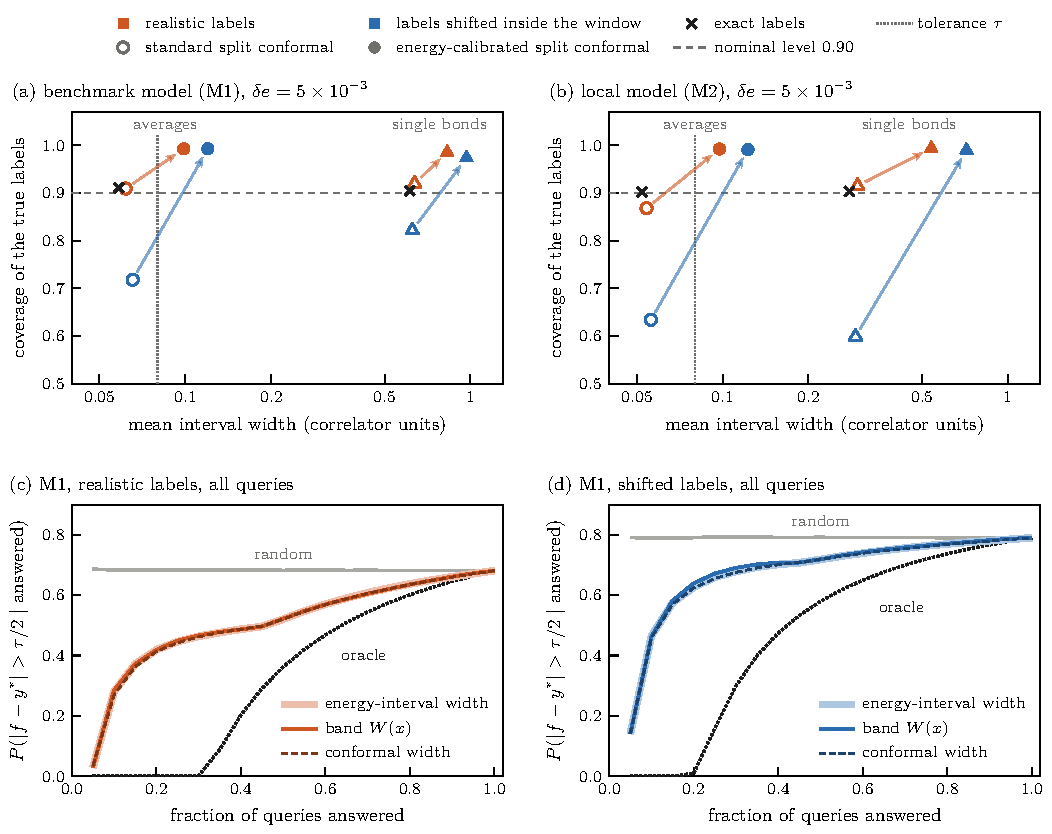
\includegraphics[width=\textwidth]{figS_learning_pgf}%
\caption{\label{fig:learnS}Learning on the public benchmark, $\de=5\times10^{-3}$, $100$ instances at $n=20$, $200$ % src: file:phase3/full_runs/learning/RESULTS.md (5e-3; 100 n = 20 instances); def:phase3/full_runs/learning/DECLARATION.md (R = 200 random splits)
splits. (a, b) Coverage of the true labels against the mean interval width, for the benchmark's model (a) and the
local model (b): averages (circles) and single bonds (triangles); realistic labels (orange) and labels shifted inside
the window (blue); open, standard split conformal calibrated on the generated labels; filled, energy-calibrated
split conformal; crosses, exact labels. Dotted: $\tau$; dashed: nominal level. (c, d) Risk--coverage curves of M1 over all
queries, with realistic (c) and shifted (d) labels: the fraction of answers that miss the truth by more than $\tau/2$, against the fraction answered, for
rankings by the energy-interval width, the band $W(x)$ and the conformal width (they coincide), random, and the oracle.
Source: deposited learning outputs.}
\end{figure}

\def\SMcap{Learning with the benchmark's model (M1). Pooled over the labels of a class, the test instances and $200$ % src: def:phase3/full_runs/learning/DECLARATION.md (R = 200 random splits)
splits; nominal level $0.90$. ``truth'': coverage of the true labels; ``own'': coverage of the labels of the set the % src: def:phase3/full_runs/learning/DECLARATION.md (0.90)
method was calibrated on; ``CSC/SC width'': ratio of mean widths; OOD: the $40$ instances with couplings in $[1,2]$. % src: file:phase3/full_runs/learning/RESULTS.md (40 declared out-of-distribution instances)
Label sets: exact; realistic generator; shifted inside the window toward less ($-$) or more ($+$) order; at the
stated $\de$.}\def\SMlab{tab:learn_m1}
\LTclearhead
% generated by figures/make_sm_learning.py from phase3/full_runs/learning/analysis/learn_M1_D_O.json -- do not edit

{\footnotesize\setlength{\tabcolsep}{4.5pt}\renewcommand{\arraystretch}{1.15}
\begin{longtable}{llcccccccc}
\caption{\SMcap}\label{\SMlab}\\
\toprule
 & & \multicolumn{2}{c}{SC} & NC & ENS & CSC & CSC/SC & SC & CSC \\ \cmidrule(lr){3-4}
labels & class & truth & own & truth & truth & truth & width & OOD & OOD \\
\midrule
exact & averages & 0.910 & 0.910 & 0.908 & 0.176 & 0.910 & -- & 0.202 & 0.202 \\
 & bonds & 0.905 & 0.905 & 0.904 & 0.158 & 0.905 & -- & 1.000 & 1.000 \\
 & diagonal pairs & 0.905 & 0.905 & 0.906 & 0.152 & 0.905 & -- & 0.990 & 0.990 \\
\addlinespace[2pt]
realistic, $10^{-3}$ & averages & 0.919 & 0.910 & 0.911 & 0.174 & 0.976 & 1.27 & 0.157 & 0.355 \\
 & bonds & 0.909 & 0.905 & 0.909 & 0.160 & 0.956 & 1.15 & 1.000 & 1.000 \\
 & diagonal pairs & 0.911 & 0.905 & 0.912 & 0.154 & 0.968 & 1.30 & 0.989 & 0.999 \\
\addlinespace[2pt]
realistic, $5\times10^{-3}$ & averages & 0.909 & 0.911 & 0.898 & 0.143 & 0.992 & 1.60 & 0.069 & 0.540 \\
 & bonds & 0.920 & 0.905 & 0.919 & 0.165 & 0.985 & 1.30 & 1.000 & 1.000 \\
 & diagonal pairs & 0.924 & 0.905 & 0.923 & 0.156 & 0.996 & 1.69 & 0.987 & 1.000 \\
\addlinespace[2pt]
shifted ($-$), $10^{-3}$ & averages & 0.887 & 0.911 & 0.875 & 0.128 & 0.966 & 1.31 & 0.054 & 0.216 \\
 & bonds & 0.889 & 0.905 & 0.891 & 0.160 & 0.949 & 1.20 & 0.996 & 1.000 \\
 & diagonal pairs & 0.905 & 0.905 & 0.901 & 0.145 & 0.972 & 1.14 & 0.921 & 0.997 \\
\addlinespace[2pt]
shifted ($-$), $5\times10^{-3}$ & averages & 0.718 & 0.911 & 0.726 & 0.077 & 0.993 & 1.83 & 0.004 & 0.417 \\
 & bonds & 0.821 & 0.904 & 0.821 & 0.143 & 0.974 & 1.55 & 0.956 & 1.000 \\
 & diagonal pairs & 0.795 & 0.905 & 0.788 & 0.093 & 0.994 & 1.36 & 0.627 & 0.999 \\
\addlinespace[2pt]
shifted ($+$), $5\times10^{-3}$ & averages & 0.707 & 0.909 & 0.720 & 0.093 & 0.995 & 2.60 & 0.550 & 0.999 \\
 & bonds & 0.785 & 0.905 & 0.788 & 0.119 & 0.989 & 1.72 & 0.993 & 1.000 \\
 & diagonal pairs & 0.669 & 0.904 & 0.671 & 0.129 & 0.996 & 3.28 & 0.992 & 1.000 \\
\addlinespace[2pt]
\bottomrule
\end{longtable}}


\def\SMcap{As Table~\ref{tab:learn_m1}, for the local model (M2).}\def\SMlab{tab:learn_m2}
\LTclearhead
% generated by figures/make_sm_learning.py from phase3/full_runs/learning/analysis/learn_M2_D_O.json -- do not edit

{\footnotesize\setlength{\tabcolsep}{4.5pt}\renewcommand{\arraystretch}{1.15}
\begin{longtable}{llcccccccc}
\caption{\SMcap}\label{\SMlab}\\
\toprule
 & & \multicolumn{2}{c}{SC} & NC & ENS & CSC & CSC/SC & SC & CSC \\ \cmidrule(lr){3-4}
labels & class & truth & own & truth & truth & truth & width & OOD & OOD \\
\midrule
exact & averages & 0.902 & 0.902 & 0.906 & 0.413 & 0.902 & -- & 0.712 & 0.712 \\
 & bonds & 0.903 & 0.903 & 0.903 & 0.594 & 0.903 & -- & 0.993 & 0.993 \\
 & diagonal pairs & 0.906 & 0.906 & 0.905 & 0.525 & 0.906 & -- & 0.985 & 0.985 \\
\addlinespace[2pt]
realistic, $10^{-3}$ & averages & 0.903 & 0.901 & 0.902 & 0.405 & 0.972 & 1.35 & 0.684 & 0.875 \\
 & bonds & 0.907 & 0.904 & 0.906 & 0.600 & 0.972 & 1.39 & 0.993 & 1.000 \\
 & diagonal pairs & 0.910 & 0.905 & 0.909 & 0.529 & 0.981 & 1.44 & 0.984 & 0.999 \\
\addlinespace[2pt]
realistic, $5\times10^{-3}$ & averages & 0.868 & 0.903 & 0.869 & 0.370 & 0.992 & 1.80 & 0.605 & 0.979 \\
 & bonds & 0.915 & 0.904 & 0.914 & 0.613 & 0.993 & 1.81 & 0.993 & 1.000 \\
 & diagonal pairs & 0.916 & 0.905 & 0.915 & 0.530 & 0.998 & 1.97 & 0.983 & 1.000 \\
\addlinespace[2pt]
shifted ($-$), $10^{-3}$ & averages & 0.842 & 0.903 & 0.845 & 0.346 & 0.967 & 1.47 & 0.539 & 0.874 \\
 & bonds & 0.847 & 0.904 & 0.836 & 0.473 & 0.967 & 1.56 & 0.963 & 0.999 \\
 & diagonal pairs & 0.860 & 0.905 & 0.851 & 0.411 & 0.973 & 1.46 & 0.947 & 0.997 \\
\addlinespace[2pt]
shifted ($-$), $5\times10^{-3}$ & averages & 0.634 & 0.904 & 0.656 & 0.188 & 0.991 & 2.19 & 0.322 & 0.985 \\
 & bonds & 0.599 & 0.903 & 0.572 & 0.198 & 0.989 & 2.45 & 0.746 & 1.000 \\
 & diagonal pairs & 0.637 & 0.905 & 0.626 & 0.171 & 0.992 & 2.14 & 0.800 & 1.000 \\
\addlinespace[2pt]
shifted ($+$), $5\times10^{-3}$ & averages & 0.645 & 0.900 & 0.667 & 0.240 & 0.997 & 2.71 & 0.885 & 1.000 \\
 & bonds & 0.552 & 0.903 & 0.530 & 0.197 & 0.995 & 2.89 & 0.716 & 1.000 \\
 & diagonal pairs & 0.550 & 0.903 & 0.526 & 0.219 & 0.999 & 4.07 & 0.900 & 1.000 \\
\addlinespace[2pt]
\bottomrule
\end{longtable}}


\def\SMcap{Abstention rules at $\tau=0.08$: answer rate / fraction of answers that miss the truth by more than % src: def:phase3/full_runs/learning/DECLARATION.md (Ï„ = 0.08)
$\tau/2$. BAND: answer iff $W(x)\le\tau$; CB: answer iff the CB interval is at most $\tau$ wide, predict its
midpoint; CSC, NC, SC: the same with those intervals; ENS: with the ensemble interval. ``inputs shifted'': the $40$ % src: file:phase3/full_runs/learning/RESULTS.md (40 declared out-of-distribution instances)
instances with couplings in $[1,2]$, where no rule is guaranteed.}\def\SMlab{tab:learn_abst}
\LTclearhead
% generated by figures/make_sm_learning.py from phase3/full_runs/learning/analysis/learn_M1/M2_D_O.json -- do not edit

{\scriptsize\setlength{\tabcolsep}{2.4pt}\renewcommand{\arraystretch}{1.15}
\begin{longtable}{llllcccccc}
\caption{\SMcap}\label{\SMlab}\\
\toprule
learner & labels & class & inputs & BAND & CB & CSC & NC & SC & ENS \\
\midrule
M1 & realistic, $5\times10^{-3}$ & averages & in & 0.998/0.031 & 0.337/0.000 & 0.333/0.000 & 0.765/0.026 & 0.815/0.026 & 1.000/0.031 \\
M1 & shifted ($-$), $5\times10^{-3}$ & averages & in & 0.995/0.142 & 0.337/0.000 & 0.225/0.009 & 0.709/0.122 & 0.773/0.125 & 1.000/0.143 \\
M1 & realistic, $5\times10^{-3}$ & averages & shifted & 0.998/0.607 & 0.340/0.017 & 0.333/0.014 & 0.880/0.577 & 0.815/0.553 & 1.000/0.607 \\
M1 & realistic, $5\times10^{-3}$ & bonds & in & 0.000/-- & 0.000/-- & 0.000/-- & 0.000/-- & 0.000/-- & 0.449/0.816 \\
M1 & realistic, $10^{-3}$ & averages & in & 0.998/0.018 & 0.467/0.007 & 0.480/0.004 & 0.803/0.015 & 0.863/0.015 & 1.000/0.018 \\
M1 & realistic, $10^{-3}$ & averages & shifted & 0.998/0.460 & 0.473/0.228 & 0.480/0.262 & 0.904/0.463 & 0.863/0.461 & 1.000/0.460 \\
M2 & realistic, $5\times10^{-3}$ & averages & in & 0.156/0.009 & 0.119/0.000 & 0.333/0.000 & 0.847/0.028 & 0.925/0.030 & 1.000/0.031 \\
M2 & shifted ($-$), $5\times10^{-3}$ & averages & in & 0.139/0.056 & 0.109/0.000 & 0.240/0.004 & 0.828/0.137 & 0.908/0.143 & 1.000/0.148 \\
M2 & realistic, $5\times10^{-3}$ & averages & shifted & 0.241/0.141 & 0.206/0.001 & 0.333/0.000 & 0.814/0.067 & 0.925/0.077 & 1.000/0.085 \\
M2 & realistic, $10^{-3}$ & averages & in & 0.779/0.013 & 0.564/0.009 & 0.588/0.011 & 0.861/0.015 & 0.943/0.017 & 1.000/0.018 \\
M2 & realistic, $10^{-3}$ & averages & shifted & 0.813/0.058 & 0.622/0.033 & 0.588/0.034 & 0.829/0.044 & 0.943/0.053 & 1.000/0.055 \\
\bottomrule
\end{longtable}}


\subsection{Held-out validation on our emulated heavy-hex labels (not the dataset's labels)}
\label{sm:heldout}

Per-site $\langle Z_i\rangle$ regressors are trained on the primary same-method labels at the grid points in
$[1.6,6.0]$ (10 points at $n=57$, 7 at $n=115$), and $\ms$ is derived from the predicted $\langle Z_i\rangle$. Models: a % src: file:phase3/full_runs/method/RESULTS.md; file:phase3/full_runs/method/laptop_post/results_tables.md; def:phase3/full_runs/method/DECLARATION.md
cubic in $1/\Jz$; a small multilayer perceptron; the simpler of the two architectures of the dataset paper, its % src: file:phase3/full_runs/method/RESULTS.md; file:phase3/full_runs/method/laptop_post/results_tables.md; def:phase3/full_runs/method/DECLARATION.md
``architecture~1'' (its Supp.\ Sec.~IV and Table~2), in our implementation: one perceptron per site with input % (structural: architecture, section and table numbers of the cited work)
$(\Jz,\dots,\Jz)$ of length equal to the number of edges, five $\tanh$ layers of width $256$, Adam with learning % src: file:phase3/full_runs/method/RESULTS.md; file:phase3/full_runs/method/laptop_post/results_tables.md; def:phase3/full_runs/method/DECLARATION.md
rate $10^{-3}$, 300 epochs, 3 seeds; our choices where that paper differs or is silent: a vector input (the % src: file:phase3/full_runs/method/RESULTS.md; file:phase3/full_runs/method/laptop_post/results_tables.md; def:phase3/full_runs/method/DECLARATION.md
parameter count of its Table~2 corresponds to a scalar one), no early stopping (it trains its final models for % (structural: table number of the cited work)
200 epochs with early stopping), raw inputs and targets, Glorot initialization, single precision. The results in % src: derived: as stated in Ref. [jaderberg2026], Supp. Sec. IV (final models: 200 epochs with early stopping; Table 2: 15,044,409 parameters = 57 x 263,937, the count for a scalar input)
the main text of the dataset paper use its geometry-aware ``architecture~2''~\cite{wanner2024}, which it reports % (structural: architecture number of the cited work)
to extrapolate with less error and which we did not implement; a nearest-neighbour null; a constant null. All are evaluated at
the held-out couplings $\Jz=1.1$--$1.4$, outside the training range. Readings declared in advance at $\Jz=1.2$: % (Jz grid values)
\emph{blind} if the perceptron models are within $3\%$ of the same-method labels and more than $9\%$ from the % src: file:phase3/full_runs/method/RESULTS.md; file:phase3/full_runs/method/laptop_post/results_tables.md; def:phase3/full_runs/method/DECLARATION.md
reference; \emph{uninformative} if the nearest-neighbour null also passes. Both hold at both sizes. The comparison is
confounded by the sparse grids: trained on DMRG labels, the dataset paper's architecture~1 (our implementation) misses the reference % (structural: architecture number of the cited work)
by $13.3\%$ ($n=57$) and $10.9\%$ ($n=115$) at $\Jz=1.2$, the small perceptron by $7.8\%$ and $10.1\%$ (last column % src: ml(57):models.ibm_arch1.rows[Jz=1.2].err_dmrgtrained_vs_dmrg_pct (13.27); ml(115):models.ibm_arch1.rows[Jz=1.2].err_dmrgtrained_vs_dmrg_pct (10.95); ml(57):models.mlp_pilot3.rows[Jz=1.2].err_dmrgtrained_vs_dmrg_pct; ml(115):models.mlp_pilot3.rows[Jz=1.2].err_dmrgtrained_vs_dmrg_pct
of each block of Table~\ref{tab:meth_learning}), whereas the cubic misses it by $0.6\%$; the dataset paper trains % src: ml(57):models.poly3_invJ.rows[Jz=1.2].err_dmrgtrained_vs_dmrg_pct (0.6)
on $45$ points. At the held-out couplings the spread of an ensemble of per-site stacks ($\le7\times10^{-4}$ in $\ms$) % src: file:phase3/STEP0_witness_prior_art_feasibility.md (45); file:phase3/full_runs/method/RESULTS.md
is about 400 times smaller than the error against the reference ($0.26$--$0.30$). % src: file:phase3/full_runs/method/RESULTS.md

\def\SMcap{Out-of-distribution test of the learners, relative $\ms$ error in percent. Each block is one model
trained on the same-method labels ($n=57$: the 10 grid points $\Jz=1.6$, $1.8$, $2.0$, $2.2$, $2.5$, $3.0$, $3.5$, % src: file:phase3/full_runs/method/RESULTS.md; file:phase3/full_runs/method/laptop_post/results_tables.md; def:phase3/full_runs/method/DECLARATION.md
$4.0$, $5.0$, $6.0$; $n=115$: the 7 points $1.6$, $2.0$, $2.5$, $3.0$, $4.0$, $5.0$, $6.0$). For each size: the error % src: file:phase3/full_runs/method/RESULTS.md; file:phase3/full_runs/method/laptop_post/results_tables.md; def:phase3/full_runs/method/DECLARATION.md
against new same-method labels (the validation a data generator can run), against the DMRG reference, and,
for comparison, the error of the same model trained on DMRG labels. Read along a row: the smooth models and the
nearest-neighbour null match the new same-method labels to within $1.5\,\%$ while missing the reference by tens of % src: file:phase3/full_runs/method/RESULTS.md; file:phase3/full_runs/method/laptop_post/results_tables.md; def:phase3/full_runs/method/DECLARATION.md
percent.}\def\SMlab{tab:meth_learning}
\LTclearhead
% generated by figures/make_sm_tables.py from phase3/full_runs/method/laptop_post/results_tables.md Table 8 (n = 57 and n = 115) -- do not edit
{\footnotesize\setlength{\tabcolsep}{5pt}\renewcommand{\arraystretch}{1.3}
\needspace{467pt}
\begin{longtable}{lcccccc}
\caption{\SMcap}\label{\SMlab}\\
\toprule
 & \multicolumn{3}{c}{$n=57$} & \multicolumn{3}{c}{$n=115$} \\ \cmidrule(lr){2-4}\cmidrule(l){5-7}
$J_z$ & \begin{tabular}[b]{@{}c@{}}vs same-\\method\end{tabular} & \begin{tabular}[b]{@{}c@{}}vs\\DMRG\end{tabular} & \begin{tabular}[b]{@{}c@{}}DMRG-trained,\\vs DMRG\end{tabular} & \begin{tabular}[b]{@{}c@{}}vs same-\\method\end{tabular} & \begin{tabular}[b]{@{}c@{}}vs\\DMRG\end{tabular} & \begin{tabular}[b]{@{}c@{}}DMRG-trained,\\vs DMRG\end{tabular} \\
\midrule
\multicolumn{7}{@{}l}{\textbf{cubic in $1/J_z$}}\\
1.1 & 1.4 & 53 & \phantom{0}1.2 & 1.2 & 53 & \phantom{0}1.0 \\
1.2 & 0.8 & 41 & \phantom{0}0.6 & 0.6 & 44 & \phantom{0}0.5 \\
1.3 & 0.3 & 33 & \phantom{0}0.3 & 0.3 & 37 & \phantom{0}0.3 \\
1.4 & 0.2 & 27 & \phantom{0}0.1 & 0.2 & 32 & \phantom{0}0.1 \\
\multicolumn{7}{@{}l}{\textbf{small multilayer perceptron}}\\
1.1 & 0.3 & 51 & 13.9 & 0.0 & 55 & 16.3 \\
1.2 & 0.2 & 41 & \phantom{0}7.8 & 0.0 & 45 & 10.1 \\
1.3 & 0.0 & 33 & \phantom{0}3.9 & 0.0 & 38 & \phantom{0}5.7 \\
1.4 & 0.0 & 27 & \phantom{0}1.5 & 0.0 & 32 & \phantom{0}2.8 \\
\multicolumn{7}{@{}l}{\textbf{per-site perceptron stack (the dataset paper's architecture~1, our implementation)}}\\
1.1 & 0.9 & 49 & 18.9 & 0.3 & 55 & 15.9 \\
1.2 & 0.7 & 39 & 13.3 & 0.2 & 45 & 10.9 \\
1.3 & 0.6 & 32 & \phantom{0}9.2 & 0.2 & 37 & \phantom{0}7.4 \\
1.4 & 0.4 & 26 & \phantom{0}6.2 & 0.2 & 31 & \phantom{0}4.8 \\
\multicolumn{7}{@{}l}{\textbf{constant null model}}\\
1.1 & 5.2 & 58 & 50.9 & 1.3 & 57 & 47.4 \\
1.2 & 4.9 & 47 & 40.2 & 1.2 & 47 & 37.9 \\
1.3 & 4.5 & 39 & 32.1 & 1.2 & 39 & 30.5 \\
1.4 & 4.3 & 32 & 25.7 & 1.1 & 33 & 24.7 \\
\multicolumn{7}{@{}l}{\textbf{nearest-neighbour null model}}\\
1.1 & 1.5 & 53 & 29.4 & 0.3 & 56 & 26.6 \\
1.2 & 1.2 & 42 & 20.3 & 0.2 & 46 & 18.5 \\
1.3 & 0.8 & 34 & 13.3 & 0.2 & 38 & 12.1 \\
1.4 & 0.6 & 27 & \phantom{0}7.8 & 0.1 & 32 & \phantom{0}7.2 \\
\bottomrule
\end{longtable}
}


\subsection{The study on emulated labels: conformal test with labels of the emulated first stage}
\label{sm:realistic}

This subsection is the study on \emph{emulated} labels that preceded the analysis of the public labels
(Sec.~\ref{sm:publiclearn}). Its labels are those of our classical emulation of the first stage of the generating
method (Sec.~\ref{sm:emu}), on our own grids of couplings, and not the dataset's labels; its truth is our DMRG
reference. It is kept in full for three reasons. It had shown, before the public labels were analysed, that standard
validation follows the labels and misses the truth. It contains the neural models, among them the dataset paper's
architecture~1 (our implementation), of which only the small network has been computed on the public labels % (structural: architecture number of the cited work)
(Sec.~\ref{sm:publiclearn}). And its
intervals are those of the in-sector map built from the published figures (Sec.~\ref{sm:map}), so its filter and its
values for Proposition~2 are DMRG-referenced numbers about emulated labels; none of them is a property of the public % (structural: proposition number)
labels. The emulated labels over-order more than the public ones, as expected from an energy error about twice
the dataset's near the isotropic point (Sec.~\ref{sm:emu}): its cubic model misses the true $\ms$ in the
test range by $4.5$--$8.8\,\tau$, against $2.28$--$3.73\,\tau$ for the public labels. % src: lib:sizes.57.models.poly3_invJ.ood_emulated.summary.miss_ms_over_tau_range (4.46, 8.78); rdl:summary.57.models.poly3_invJ.real.test.miss_tau (2.2860, 3.7202); file:phase3/full_runs/real_data/results/RESULTS_learn.md (2.28-3.73, rounded outward)

\emph{Design} (written in the script header before any of its outputs was read, but after the held-out numbers of
Sec.~\ref{sm:heldout} were known; unlike the other computations it was not time-stamped, and the script was edited
after an initial quick run of the cubic and null models, whose numbers the final run reproduces exactly). Data: every coupling at which we have both an emulated state of the first stage (primary
variant) and a DMRG reference, all stored, nothing recomputed: $14$ at $n=57$ ($10$ in the training range $\Jz\ge1.6$, and $1.1$--$1.4$) and $11$ at % src: file:phase3/full_runs/learning_ibm/README.md (14 couplings; 10 training; 11 couplings)
$n=115$ ($7$ and $4$). The emulated labels are those of real states and agree with their energies, which are their % src: file:phase3/full_runs/learning_ibm/README.md (7 training; 4 test)
Rayleigh quotients. Labels: per-site $\langle Z_i\rangle$ and $\ms$ derived from them. Models: those of
Sec.~\ref{sm:heldout}, imported unchanged from the deposited method code. Calibration: standard conformal at
$\alpha=0.1$ on held-out emulated labels, each training coupling held out in turn; the interval is the prediction of % src: lib:alpha (0.1)
the model trained on all training couplings $\pm q$, with $q$ the $\lceil(1-\alpha)(N+1)\rceil$-th smallest held-out
residual ($N$ residuals; pooled over sites for $\langle Z_i\rangle$). This is the plain jackknife, not the
jackknife+ of Ref.~\cite{barber2019}, and it has no finite-sample guarantee~\cite{barber2019}. For $\ms$, with $N=9$ or $10$ couplings at $n=57$, % src: file:phase3/full_runs/learning_ibm/README.md (10 training); derived: 10 - 1 = 9
$q$ is the maximum residual and the level $0.9$ is just attainable; with $7$ couplings at $n=115$ it is not, the % src: file:phase3/full_runs/learning_ibm/README.md (7 training); lib:alpha (0.1); derived: 1 - alpha = 0.9
level is $N/(N+1)$ and the maximum residual is used. This is a statement about the index of the quantile: with the
plain jackknife no level is guaranteed at any $N$, and the couplings are a fixed grid, to which the exchangeability
assumed in Proposition~2 applies only in the sense of a held-out coupling drawn at random. The $57$ site residuals of one coupling are dependent, so the % (structural: proposition number; n = 57)
effective calibration size is the number of couplings. Tests: at $1.1$--$1.4$ (model and $q$ % src: lib:alpha (0.1); derived: 1 - alpha = 0.9; lib:ood (1.1, 1.4)
from all training couplings) and in the training range (one coupling held out as test, model and $q$ from the
others, repeated over the held-out coupling). Coverage of the new emulated labels (primary variant; also a second
emulated state, without the noise floor, at the same coupling) and of the DMRG truth. Control: the same with DMRG
labels for training and calibration. Widths and misses in units of $\tau=0.06|o_\GS|$, per site for $\langle Z_i\rangle$. % src: def:phase3/full_runs/map/DECLARATION.md (tau = 0.06|O_GS|)
Certified status at each label's own energy $\epsilon_{\rm emu}$: certified iff $\epsilon_{\rm emu}$ is at most the
map's $\epsilon_\tau$ (outer side) for that label and coupling; width bounds from the stored windows, since a window
only grows with the energy; local labels use the map's bulk and boundary site rows; couplings without a map row
($\Jz=2.2$ and $3.5$ at $n=57$) abstain by default. Robustness: a single split with $3$ ($n=57$) or $2$ ($n=115$) held-out calibration couplings, all choices, for % src: lib:sizes.57.split_robustness_ood.poly3_invJ.k_cal (3); lib:sizes.115.split_robustness_ood.poly3_invJ.k_cal (2)
the cubic model and the nearest-neighbour null.

\def\SMcap{Learning test on emulated labels of the heavy-hex model. Standard conformal intervals at nominal level $0.9$, % src: lib:alpha (0.1); derived: 1 - alpha
calibrated on held-out emulated labels (left block) or, as a control, on DMRG labels (right block). ``training
range'': each training coupling held out as test in turn; ``1.1--1.4'': the test range. Coverage of the new emulated % src: lib:ood (1.1, 1.4)
site labels and of the true (DMRG) site labels and $\ms$; median width of the $\ms$ interval and range of its miss of the
true $\ms$, in units of $\tau$. The dataset paper's architecture~1 (our implementation) was run on the test range only.}\def\SMlab{tab:learn_emu} % (structural: architecture number of the cited work)
\LTclearhead
% copy (all lines but this one) of the generated table of the study on emulated labels (its generator is named in the first line of the original file), with one block heading renamed (R11: the dataset paper's architecture 1, our implementation); copied by figures/sm_tables/make_rdlearn.py so that the file name read by the Supplement holds no company name -- do not edit
{\footnotesize\setlength{\tabcolsep}{4pt}\renewcommand{\arraystretch}{1.25}
\begin{longtable}{llcccccc}
\caption{\SMcap}\label{\SMlab}\\
\toprule
 & & \multicolumn{4}{c}{trained on emulated labels} & \multicolumn{2}{c}{trained on DMRG labels} \\ \cmidrule(lr){3-6}\cmidrule(l){7-8}
$n$ & test & \begin{tabular}[b]{@{}c@{}}sites: covers\\new emulated\end{tabular} & \begin{tabular}[b]{@{}c@{}}sites: covers\\truth\end{tabular} & \begin{tabular}[b]{@{}c@{}}$m_s$: covers\\truth\end{tabular} & \begin{tabular}[b]{@{}c@{}}$m_s$: width, miss\\(units of $\tau$)\end{tabular} & \begin{tabular}[b]{@{}c@{}}sites: covers\\truth\end{tabular} & \begin{tabular}[b]{@{}c@{}}$m_s$: miss\\(units of $\tau$)\end{tabular} \\
\midrule
\multicolumn{8}{@{}l}{\textbf{cubic in $1/J_z$}}\\
57 & training range & 0.90 & 0.10 & 0.10 & 0.09; 0.02--3.05 & 0.89 & 0.00--0.01 \\
57 & 1.1--1.4 & 0.31 & 0.00 & 0.00 & 0.13; 4.46--8.78 & 0.07 & 0.02--0.20 \\
115 & training range & 0.91 & 0.00 & 0.00 & 0.04; 0.06--3.82 & 0.86 & 0.00--0.03 \\
115 & 1.1--1.4 & 0.06 & 0.00 & 0.00 & 0.06; 5.25--8.91 & 0.17 & 0.02--0.17 \\
\multicolumn{8}{@{}l}{\textbf{small perceptron}}\\
57 & training range & 0.93 & 0.20 & 0.20 & 0.04; 0.01--3.00 & 0.90 & 0.00--0.16 \\
57 & 1.1--1.4 & 0.34 & 0.00 & 0.00 & 0.04; 4.43--8.50 & 0.00 & 0.26--2.31 \\
115 & 1.1--1.4 & 0.93 & 0.00 & 0.00 & 0.05; 5.28--9.22 & 0.31 & 0.46--2.72 \\
\multicolumn{8}{@{}l}{\textbf{per-site perceptron stack (the dataset paper's architecture~1, our implementation)}}\\
57 & 1.1--1.4 & 0.43 & 0.00 & 0.00 & 0.10; 4.34--8.20 & 0.00 & 1.03--3.15 \\
\multicolumn{8}{@{}l}{\textbf{nearest-neighbour null}}\\
57 & training range & 0.91 & 0.47 & 0.50 & 0.47; 0.02--3.13 & 0.92 & 0.14--0.91 \\
57 & 1.1--1.4 & 0.79 & 0.00 & 0.00 & 0.60; 4.55--8.79 & 0.06 & 1.30--4.90 \\
115 & training range & 0.86 & 0.27 & 0.29 & 0.20; 0.01--3.89 & 0.90 & 0.13--1.48 \\
115 & 1.1--1.4 & 1.00 & 0.00 & 0.00 & 0.25; 5.31--9.31 & 0.33 & 1.19--4.44 \\
\bottomrule
\end{longtable}}


\emph{Results} (Table~\ref{tab:learn_emu}). With the cubic model at $n=57$ the intervals cover $0.90$ of the new % src: lib:sizes.57.models.poly3_invJ.indist_emulated.summary.covZ_emu (0.904)
emulated site labels in the training range and $0.10$ of the true ones; at $1.1$--$1.4$, $0.31$ of the new emulated % src: lib:sizes.57.models.poly3_invJ.indist_emulated.summary.covZ_truth (0.100); lib:sizes.57.models.poly3_invJ.ood_emulated.summary.covZ_emu (0.311); lib:ood (1.1, 1.4)
labels and none of the true ones; the second emulated state at the same couplings is covered at $0.46$ and $0.02$: % src: lib:sizes.57.models.poly3_invJ.indist_emulated.summary.covZ_ideal (0.458); lib:sizes.57.models.poly3_invJ.ood_emulated.summary.covZ_ideal (0.022)
a slightly different setting of the same generator already escapes the narrow intervals. The prediction of $\ms$
misses the truth there by $27$--$53\%$ and the new emulated labels by at most $1.4\%$; trained on DMRG labels, the same % src: lib:sizes.57.models.poly3_invJ.ood_emulated.summary.err_ms_vs_truth_pct_range (26.8, 52.7); lib:sizes.57.models.poly3_invJ.ood_emulated.summary.err_ms_vs_emu_pct_max (1.445)
model misses the truth by $0.1$--$1.2\%$. The nearest-neighbour null, with wider intervals, covers $0.79$ of the new % src: lib:sizes.57.models.poly3_invJ.ood_exact_control.summary.err_ms_vs_truth_pct_range (0.13, 1.20); lib:sizes.57.models.null_nn.ood_emulated.summary.covZ_emu (0.785)
emulated labels at $1.1$--$1.4$ and none of the true ones. With a single split, the cubic model covers $0.22$ of the % src: lib:sizes.57.models.null_nn.ood_emulated.summary.covZ_truth (0.0); lib:sizes.57.split_robustness_ood.poly3_invJ.covZ_emu (0.217); lib:ood (1.1, 1.4)
new emulated labels and none of the true ones in the test range, over all $120$ choices of the calibration % src: lib:sizes.57.split_robustness_ood.poly3_invJ.covZ_truth (0.0); lib:sizes.57.split_robustness_ood.poly3_invJ.n_splits (120)
couplings. At $n=115$ (an emulation that misses its energy condition) the cubic model covers $0.91$ of the new emulated % src: lib:sizes.115.models.poly3_invJ.indist_emulated.summary.covZ_emu (0.912)
site labels in the training range and none of the true values in either range.
The small perceptron gives the same picture: at $n=57$ it covers $0.93$ and $0.20$ of the new emulated and the true % src: lib:sizes.57.models.mlp_pilot3.indist_emulated.summary.covZ_emu (0.926); lib:sizes.57.models.mlp_pilot3.indist_emulated.summary.covZ_truth (0.200)
site labels in the training range and $0.34$ and $0$ in the test range; at $n=115$, $0.93$ and $0$ in the test range. % src: lib:sizes.57.models.mlp_pilot3.ood_emulated.summary.covZ_emu (0.338); lib:sizes.57.models.mlp_pilot3.ood_emulated.summary.covZ_truth (0.0); lib:sizes.115.models.mlp_pilot3.ood_emulated.summary.covZ_emu (0.933); lib:sizes.115.models.mlp_pilot3.ood_emulated.summary.covZ_truth (0.0)
Its exact-label control misses the true $\ms$ in the test range by up to $2.3\,\tau$ ($n=57$) and $2.7\,\tau$ % src: lib:sizes.57.models.mlp_pilot3.ood_exact_control.summary.miss_ms_over_tau_range (2.31); lib:sizes.115.models.mlp_pilot3.ood_exact_control.summary.miss_ms_over_tau_range (2.72)
($n=115$), so for this model part of the miss is model error; the label error still dominates ($4.4$--$9.2\,\tau$). % src: lib:sizes.57.models.mlp_pilot3.ood_emulated.summary.miss_ms_over_tau_range (4.43); lib:sizes.115.models.mlp_pilot3.ood_emulated.summary.miss_ms_over_tau_range (9.22)
The dataset paper's architecture~1 (our implementation), % (structural: architecture number of the cited work)
run at $n=57$ in the test range only, covers $0.43$ of the new emulated site labels % src: lib:sizes.57.models.ibm_arch1.ood_emulated.summary.covZ_emu (0.425)
and none of the true ones, missing $\ms$ by $4.3$--$8.2\,\tau$ ($26$--$49\%$); its exact-label control misses by % src: lib:sizes.57.models.ibm_arch1.ood_emulated.summary.miss_ms_over_tau_range (4.34, 8.20); lib:sizes.57.models.ibm_arch1.ood_emulated.summary.err_ms_vs_truth_pct_range (26.0, 49.2)
$1.0$--$3.1\,\tau$ ($6.2$--$18.9\%$) on our $10$ training couplings, the model error noted in Sec.~\ref{sm:heldout}. % src: lib:sizes.57.models.ibm_arch1.ood_exact_control.summary.miss_ms_over_tau_range (1.03, 3.15); lib:sizes.57.models.ibm_arch1.ood_exact_control.summary.err_ms_vs_truth_pct_range (6.2, 18.9); file:phase3/full_runs/learning_ibm/README.md (10 training)
For cost, this architecture was run at $n=57$ only. % (sizes)

\emph{Further numbers of this study} (in the main text before the public labels were analysed). At $n=57$ every % (sizes)
model evaluated in the training range (the cubic, the small network and the nearest-neighbour null) misses the
true $\ms$ by more than $\tau/2$ at the five couplings $\Jz=1.6$--$2.5$, by more than $\tau$ at $1.6$--$2.0$ % src: ldsc:label_error_57.couplings_all_models_gt_half_tau (1.6, 2.5); file:phase3/full_runs/learning_ibm/out/descriptive.json (1.6, 2.0)
(the cubic model by up to $3.1\,\tau$, at $\Jz=1.6$) and by % src: lib:sizes.57.models.poly3_invJ.indist_emulated.summary.miss_ms_over_tau_range (3.05); derived: upper bound 3.0511 ceiled to 3.1
less than $\tau/2$ at $\Jz=3.0$--$6.0$; the emulated labels themselves miss it by $0.68$--$3.0\,\tau$ and % src: ldsc:label_error_57.couplings_no_model_gt_half_tau (3.0, 6.0); ldsc:label_error_57.rows (0.676, 3.010)
$0.02$--$0.32\,\tau$ there. The cubic model's intervals are $0.09\,\tau$ wide (median) in the training range and % src: ldsc:label_error_57.rows (0.021, 0.316); lib:sizes.57.models.poly3_invJ.indist_emulated.summary.widthM_tau_median (0.093)
$0.13\,\tau$ in the test range, where it misses $\ms$ by $4.5$--$8.8\,\tau$; trained and calibrated on exact % src: lib:sizes.57.models.poly3_invJ.ood_emulated.summary.widthM_tau_median (0.126); lib:sizes.57.models.poly3_invJ.ood_emulated.summary.miss_ms_over_tau_range (4.46, 8.78)
labels its intervals ($0.03\,\tau$) cover none of the true $\ms$ there either, as no method has a guarantee under % src: lib:sizes.57.models.poly3_invJ.ood_exact_control.summary.widthM_tau_median (0.026); lib:sizes.57.models.poly3_invJ.ood_exact_control.summary.covM_truth (0.0)
a shift of the input, but they miss it by at most $0.21\,\tau$. The null's intervals, $0.47\,\tau$ wide, cover % src: lib:sizes.57.models.poly3_invJ.ood_exact_control.summary.miss_ms_over_tau_range (0.2005); derived: upper bound 0.2005 ceiled to 0.21; lib:sizes.57.models.null_nn.indist_emulated.summary.widthM_tau_median (0.474)
$50\%$ of the true values of $\ms$ in the training range. In the test range the intervals of the small network % src: lib:sizes.57.models.null_nn.indist_emulated.summary.covM_truth (0.5)
are $0.04\,\tau$ wide and those of the dataset paper's % src: lib:sizes.57.models.mlp_pilot3.ood_emulated.summary.widthM_tau_median (0.045)
architecture~1 % (structural: architecture number of the cited work)
$0.10\,\tau$; at $n=115$ those of the cubic % src: lib:sizes.57.models.ibm_arch1.ood_emulated.summary.widthM_tau_median (0.102)
model are $0.04\,\tau$ wide. The coverage of $0.90$ of the new emulated site labels in the training range is an % src: lib:sizes.115.models.poly3_invJ.indist_emulated.summary.widthZ_tau_median (0.038); lib:sizes.57.models.poly3_invJ.indist_emulated.summary.covZ_emu (0.904)
average over the ten held-out couplings: $0.96$--$1.00$ at the eight interior ones, and $0.789$ and $0.298$ at % src: file:paper/reviews/R10_2026-11-12/scratch/math-learning/calibration_variants_out.txt (0.965, 1.000; 0.789; 0.298)
$\Jz=1.6$ and $6.0$, where leaving a coupling out is an extrapolation (recomputation of an internal review). With the % (Jz grid values)
jackknife+ and the jackknife-minmax variants~\cite{barber2019}, whose levels under exchangeability are $1-2\alpha$
and $1-\alpha$, the result for $\ms$ is the same as with the plain jackknife: $9$ of $10$ new emulated values and % src: file:paper/reviews/R10_2026-11-12/scratch/math-learning/calibration_variants_out.txt (covers new emulated m_s at 9 of 10)
$1$ of $10$ true values covered, with median widths $0.096$ and $0.114\,\tau$. % src: file:paper/reviews/R10_2026-11-12/scratch/math-learning/calibration_variants_out.txt (the true m_s at 1 of 10; median width 0.096 tau; median width 0.114 tau)

\emph{The label filter.} At the labels' own energies the map certifies $\ms$ at $\Jz=4.0$, $5.0$, % src: lib:sizes.57.abstention.answered_m_s (4.0, 5.0, 6.0)
$6.0$ ($n=57$) and $5.0$, $6.0$ ($n=115$; at $4.0$ the emulated energy error, $0.85$, exceeds the map's $0.66$), and % src: lib:sizes.115.abstention.answered_m_s (5.0, 6.0); lib:sizes.115.certification.4.0.eps_emu (0.852); lib:sizes.115.certification.4.0.m_s.eps_tau_out (0.659); lib:sizes.115.train (4.0)
the site labels only at $\Jz=6.0$ ($n=57$). The filter therefore answers $\ms$ at $21\%$ ($n=57$) and $18\%$ ($n=115$) of % src: lib:sizes.57.abstention.answered_local (6.0); lib:sizes.57.abstention.frac_m_s (0.214); lib:sizes.115.abstention.frac_m_s (0.182)
the couplings ($3$ of $14$ and $2$ of $11$) and none in the test range, where the energy interval of $\ms$ is at least $11.3$--$17.3\,\tau$ % src: lib:sizes.57.abstention.frac_m_s_ood (0.0); lib:sizes.57.abstention.m_s_certified_width_tau_ge_ood (11.33, 17.28); lib:sizes.57.abstention.answered_m_s (3 couplings); lib:sizes.115.abstention.answered_m_s (2 couplings); file:phase3/full_runs/learning_ibm/README.md (14 couplings; 11 couplings)
($n=57$) and $10.3$--$15.3\,\tau$ ($n=115$) wide, and that of the bulk site at least $35$--$50\,\tau$. Its answers % src: lib:sizes.115.abstention.m_s_certified_width_tau_ge_ood (10.26, 15.28); lib:sizes.57.abstention.Z_bulk_certified_width_tau_ge_ood (35.03, 50.40)
miss the truth by at most $0.44\%$ ($0.073\,\tau$) at $n=57$ and $0.83\%$ ($0.14\,\tau$) at $n=115$ (cubic model). % src: lib:sizes.57.abstention.poly3_invJ.max_err_answered_pct (0.437); lib:sizes.57.abstention.poly3_invJ.max_miss_over_tau_answered (0.0728); lib:sizes.115.abstention.poly3_invJ.max_err_answered_pct (0.82065); derived: upper bound 0.82065 ceiled to 0.83 (R9, 2026-11-11); lib:sizes.115.abstention.poly3_invJ.max_miss_over_tau_answered (0.137)
The width bounds use stored windows at energies below the emulated ones, so they are lower bounds: they are the
stored map rows at the last stored energy below the label's. The hull of the stored states at the label's own
energy gives the greater lower bounds $16.8$--$21.3\,\tau$ at $n=57$ (Table~\ref{tab:learn_prop2}); each of the % src: lp2:sizes.57.intervals.1.4.w_in_tau (16.87); lp2:sizes.57.intervals.1.1.w_in_tau (21.36); derived: lower bounds floored to 16.8 and 21.3
values quoted for this quantity is a valid lower bound. The energy
intervals contain the truth by construction under the assumptions of Table~I of the main text. At $\Jz=2.2$ and $3.5$ % src: lp2:sizes.57.missing_rows (2.2, 3.5)
($n=57$) the map has no computed row and the filter abstains by default; with $\epsilon_\tau$ interpolated
log-linearly in $\Jz$, as for $J^*$, $2.2$ stays uncertified (emulated excess $0.64$ against $0.041$) and $3.5$ is % src: lp2:sizes.57.label_filter_interp.2.2.eps_emu (0.638); lp2:sizes.57.label_filter_interp.2.2.eps_tau_out_interp (0.0406)
certified ($0.126$ against $0.192$). The filter keeps no label that misses the truth by more than $\tau/2$; it % src: lp2:sizes.57.label_filter_interp.3.5.eps_emu (0.1256); lp2:sizes.57.label_filter_interp.3.5.eps_tau_out_interp (0.1920)
also drops $\Jz=3.0$ and $3.5$, whose labels are within $0.32$ and $0.16\,\tau$ of the truth. % src: ldsc:label_error_57.rows (0.316, 0.162)
At $\Jz=3.0$ the emulated energy is above the map's threshold; at $\Jz=3.5$ there is no computed row. % (Jz grid values)
What the filter guarantees for a kept label is that it lies within its energy interval's width of the truth, and
here that is more than the observation above: at their own energies the three kept labels at $n=57$ have energy % (sizes)
intervals at most $0.50$, $0.26$ and $0.16\,\tau$ wide, whose farther ends lie at most $0.37$, $0.18$ and % src: file:paper/reviews/R10_2026-11-12/scratch/math-learning/extra_checks_out.txt (w_out 0.494, 0.254, 0.158; guaranteed <= 0.361, 0.174); derived: upper bounds ceiled to two decimals
$0.11\,\tau$ from the label; each kept label is therefore guaranteed within $0.37\,\tau$ of the truth, under the % src: file:paper/reviews/R10_2026-11-12/scratch/math-learning/extra_checks_out.txt (guaranteed <= 0.106; max guaranteed distance kept 0.361 tau); derived: upper bounds ceiled to two decimals
assumptions of Table~I of the main text, and is in fact within $0.09\,\tau$ (recomputation of an internal review). % src: file:paper/reviews/R10_2026-11-12/scratch/math-learning/extra_checks_out.txt (max label error kept 0.089 tau); derived: upper bound 0.089 ceiled to 0.09

\emph{Proposition~2 for the cubic model} (Table~\ref{tab:learn_prop2}; design note % (structural: proposition number)
\texttt{PROP2\_DESIGN.md} in the deposited folder of this study, time-stamped before its script was written; script
\texttt{code/\allowbreak prop2\_cubic.py}). The filter above needs a generated label and its energy at the query.
Proposition~2 of the main text instead uses only the energy intervals of the training labels. The cubic model is % (structural: proposition number)
linear in its labels, $\hat m_s(x)=\sum_ja_j(x)\,m_{s,j}$ with the same $a(x)$ for every site; these coefficients
reproduce the fitted model's predictions to $2\times10^{-13}$. Each training label's energy interval is the map's window of $\ms$ at the % src: lp2:sizes.57.linearity_check_max_abs (2.0e-13)
label's own energy, from the stored chains (outer side, DMRG-referenced) and the stored explicit states (inner
side); every label and every true value lies in its outer interval. The band $W(x)$ of (a) and the scores of (b),
$s_j=\max_{y\in I_j}|f_{-j}(x_j)-y|$, use the same leave-one-coupling-out calibration as the standard intervals; lower
values use the inner widths (zero, and the label itself, at the two couplings without a map row), upper values the
outer widths (interpolated there, marked as indicative). At $n=57$ the intervals of (b) are at least % src: def:phase3/full_runs/map/DECLARATION.md (n = 57)
$16.5$--$22.4\,\tau$ wide in the training range and $25.1$--$30.1\,\tau$ in the test range, and $W(x)$ is at least % src: lp2:sizes.57.summary.width_b_lo_tau_indist (16.55, 22.36); lp2:sizes.57.summary.width_b_lo_tau_ood (25.05, 30.07)
$1.15$--$24.1\,\tau$ and $41.9$--$249\,\tau$; at $n=115$, $22.1$--$32.6\,\tau$ and $38.0$--$44.9\,\tau$ for (b). Rule % src: lp2:sizes.57.summary.W_lo_tau_indist (1.153, 24.12); lp2:sizes.57.summary.W_lo_tau_ood (41.93, 249.4); lp2:sizes.115.summary.width_b_lo_tau_indist (22.09, 32.57); lp2:sizes.115.summary.width_b_lo_tau_ood (38.03, 44.94)
(c) therefore answers none of the $14$ ($n=57$) and $11$ ($n=115$) couplings, at every one of them definitely, % src: lp2:sizes.57.summary.n_queries (14); lp2:sizes.115.summary.n_queries (11)
since even the lower values exceed $\tau$. The intervals of (b) cover the truth at every coupling. The widths are set
by the labels near the isotropic point: their energy intervals are $11.7$--$12.7\,\tau$ wide at $\Jz=1.6$ ($n=57$, % src: lp2:sizes.57.intervals.1.6.w_in_tau (11.70); lp2:sizes.57.intervals.1.6.w_out_tau (12.68)
at the emulated energy), and every prediction of a cubic fit depends on them. Trained on all ten training labels,
the cubic model has $W(x)=0.88$--$1.16\,\tau$ at $\Jz=5.0$ and $2.1$--$2.9\,\tau$ at $4.0$ and $6.0$, so that at % src: lp2:sizes.57.in_sample_all_R (0.88, 1.16, 2.11, 2.93)
$\Jz=5.0$ the stored windows do not decide whether its band exceeds $\tau$. % (Jz grid value)
These are values for one model and the constant-width score. The labels at $\Jz=1.6$--$2.5$ carry
$72.5$--$97.1\%$ of the lower value of $W(x)$ at the couplings examined and set the greatest calibration score. % src: file:paper/reviews/R10_2026-11-12/scratch/math-learning/extra_checks_out.txt (72.5 %; 97.1 %)
They do not show that a learner trained on uncertified labels cannot certify a prediction: Proposition~2 gives % (structural: proposition number)
sufficient conditions, its part (b) puts no condition on the training labels, and on the public labels a control
model trained on uncertified labels as well passes the constructive test (Sec.~\ref{sm:publiclearn}). What decides
is the calibration set, through the floor of part (d).

\emph{The floor for the emulated labels} (Proposition~\ref{prop:floor}; values recomputed by two independent codes
of an internal review; widths in units of the tolerance at the query). At $n=57$ the lower values of the energy % (sizes)
intervals (hulls of stored explicit states; $0$ at the two couplings without a map row) are $11.7$, $7.8$, $5.6$, % src: lp2:sizes.57.intervals.1.6.w_in_tau (11.70); lp2:sizes.57.intervals.1.8.w_in_tau (7.83); lp2:sizes.57.intervals.2.0.w_in_tau (5.57); lp2:sizes.57.missing_rows (2 rows, width 0)
$2.3$, $1.3$, $0.49$, $0.25$ and $0.15$ tolerances wide at $\Jz=1.6$, $1.8$, $2.0$, $2.5$, $3.0$, $4.0$, $5.0$ and % src: lp2:sizes.57.intervals.2.5.w_in_tau (2.34); lp2:sizes.57.intervals.3.0.w_in_tau (1.32); lp2:sizes.57.intervals.4.0.w_in_tau (0.494); lp2:sizes.57.intervals.5.0.w_in_tau (0.253); lp2:sizes.57.intervals.6.0.w_in_tau (0.145)
$6.0$. With nine calibration couplings the floor is the widest of the nine lower widths: for any learner the % (Jz grid value)
interval is at least $8.25\,\tau$ wide when $\Jz=1.6$ is the held-out coupling and $9.18$--$11.09\,\tau$ otherwise, % src: file:paper/reviews/R10_2026-11-12/scratch/break-lemmas/break_F_out.txt (8.254; 9.183 .. 11.093; floored)
and $12.61$--$15.13\,\tau$ in the test range (ten calibration couplings). The cubic model's intervals are $1.980$ % src: file:paper/reviews/R10_2026-11-12/scratch/break-lemmas/break_F_out.txt (12.615 .. 15.139, floored; 1.980)
to $2.015$ times the floor at every coupling, because its predictions sit near the upper ends of the widest % src: file:paper/reviews/R10_2026-11-12/scratch/break-lemmas/break_F_out.txt (2.015)
intervals. At $n=115$ the level $0.9$ is not attainable with the six (training range) or seven (test range) % src: lib:alpha (0.1); derived: 1 - alpha = 0.9
calibration couplings: the index $k$ exceeds their number, so $q=+\infty$. For the greatest score, which is what the
jackknife reports there and whose nominal level is $6/7$ and $7/8$, the floor is $10.27$--$15.29\,\tau$ and % src: file:paper/reviews/R10_2026-11-12/scratch/break-lemmas/break_F_out.txt (10.278 .. 15.299, floored)
$17.84$--$21.09\,\tau$. % src: file:paper/reviews/R10_2026-11-12/scratch/rw-V/v_item45_out.txt (17.8498, 21.0944; floored)

\emph{A width-normalized score on the same intervals} (an illustration of Proposition~\ref{prop:floor}(v), from an
internal review; not a result for the trained models). On the eight couplings with a map row at $n=57$, holding out each % (sizes)
in turn and using the greatest of the seven scores, the score $|f-y|/\sigma(x)$ with $\sigma$ a power law in $\Jz$
fitted to the eight widths and with predictions at the centres of the intervals gives intervals of $12.38$, % src: file:paper/reviews/R10_2026-11-12/scratch/break-lemmas/break_F_out.txt (1.6: 12.38)
$8.08$, $5.49$, $2.58$, $1.40$, $0.54$, $0.26$ and $0.15$ tolerances. They contain the query's whole energy % src: file:paper/reviews/R10_2026-11-12/scratch/break-lemmas/break_F_out.txt (1.6: 12.38, 1.8: 8.08, 2.0: 5.49*, 2.5: 2.58, 3.0: 1.40, 4.0: 0.54, 5.0: 0.26, 6.0: 0.15)
interval at seven of the eight couplings (all but $\Jz=2.0$), as part (iii) requires, and rule (c) answers at $\Jz=4.0$, $5.0$ and
$6.0$, the couplings at which the label filter answers, although only three of the eight intervals are narrower % (Jz grid value)
than the tolerance. The learner is idealized: the example shows that the condition of part (iv) on the calibration
labels is special to the constant-width score.

\emph{The dataset's own training set, as estimated from the figures.} Before the public energies were used, the
floor had been evaluated for the dataset's $45$ training points from the figures-based map. With $45$ calibration
labels at level $0.9$ at most three labels may be wider than the interval, and that map has four computed % src: lib:alpha (0.1); derived: 1 - alpha = 0.9
couplings ($\Jz\le2.5$) whose energy intervals are at least $0.095$ wide at $n=57$, so the interval of any learner % src: file:paper/reviews/R10_2026-11-12/scratch/break-lemmas/break_F_out.txt (0.09507)
was at least $1.6$ times the greatest tolerance of the training range ($1.4$ times at $n=115$), conditional on % src: file:paper/reviews/R10_2026-11-12/scratch/break-lemmas/break_F_out.txt (ratio 1.6146; ratio 1.4887)
the digitized energies and on in-sector states. The public energies replace this estimate by the values of
Sec.~\ref{sm:publiclearn}.

\needspace{400pt} % (layout: keeps the table below on one page)
\def\SMcap{Proposition~2 for the cubic model on the emulated labels, from the stored windows at each label's energy. Training couplings: % (structural: proposition number)
model and calibration without the coupling (in distribution); test couplings ($1.1$--$1.4$): model and calibration on % src: lib:ood (1.1, 1.4)
all training couplings. Each entry is a lower and an upper value: lower from the inner widths (zero at a coupling
without a map row), upper from the outer widths; $^\dagger$: the upper value uses widths interpolated at $\Jz=2.2$ % src: lp2:sizes.57.missing_rows (2.2, 3.5)
and $3.5$ ($n=57$) and is indicative. Rule (c): answer iff the upper width of (b) is at most $\tau$.}\def\SMlab{tab:learn_prop2} % src: lp2:sizes.57.missing_rows (2.2, 3.5)
\LTclearhead
% generated by figures/make_sm_learning_prop2.py from phase3/full_runs/learning_ibm/out/prop2_cubic.json -- do not edit
{\footnotesize\setlength{\tabcolsep}{4pt}\renewcommand{\arraystretch}{1.2}
\begin{longtable}{llccccc}
\caption{\SMcap}\label{\SMlab}\\
\toprule
$n$ & $J_z$ & \begin{tabular}[b]{@{}c@{}}label's energy\\interval, $w/\tau$\end{tabular} & \begin{tabular}[b]{@{}c@{}}band (a)\\$W(x)/\tau$\end{tabular} & \begin{tabular}[b]{@{}c@{}}interval (b)\\width $2q/\tau$\end{tabular} & \begin{tabular}[b]{@{}c@{}}miss of $m_s$\\(units of $\tau$)\end{tabular} & rule (c) \\
\midrule
57 & 1.6 & 11.7--12.7 & 24.1--32.1$^\dagger$ & 16.5--17.0$^\dagger$ & 3.05 & abstain \\
57 & 1.8 & 7.83--8.62 & 7.00--9.17$^\dagger$ & 22.4--23.0$^\dagger$ & 2.10 & abstain \\
57 & 2.0 & 5.57--6.04 & 4.49--7.06$^\dagger$ & 21.2--21.8$^\dagger$ & 1.50 & abstain \\
57 & 2.2 & no map row & 6.97--7.65$^\dagger$ & 20.6--21.2$^\dagger$ & 1.09 & abstain \\
57 & 2.5 & 2.34--2.66 & 3.83--5.55$^\dagger$ & 19.9--20.5$^\dagger$ & 0.69 & abstain \\
57 & 3.0 & 1.32--1.35 & 1.51--2.57$^\dagger$ & 19.3--19.8$^\dagger$ & 0.34 & abstain \\
57 & 3.5 & no map row & 3.37--3.76$^\dagger$ & 18.9--19.4$^\dagger$ & 0.16 & abstain \\
57 & 4.0 & 0.49--0.49 & 3.17--3.87$^\dagger$ & 18.7--19.2$^\dagger$ & 0.07 & abstain \\
57 & 5.0 & 0.25--0.25 & 1.15--1.56$^\dagger$ & 18.4--18.9$^\dagger$ & 0.02 & abstain \\
57 & 6.0 & 0.15--0.16 & 7.19--8.04$^\dagger$ & 18.2--18.7$^\dagger$ & 0.06 & abstain \\
57 & 1.1 (test) & 21.4--35.6 & 249--310$^\dagger$ & 30.1--30.9$^\dagger$ & 8.78 & abstain \\
57 & 1.2 (test) & 19.8--28.8 & 139--173$^\dagger$ & 27.9--28.7$^\dagger$ & 6.91 & abstain \\
57 & 1.3 (test) & 19.0--23.2 & 77.5--95.5$^\dagger$ & 26.3--27.1$^\dagger$ & 5.52 & abstain \\
57 & 1.4 (test) & 16.9--18.9 & 41.9--51.2$^\dagger$ & 25.1--25.7$^\dagger$ & 4.46 & abstain \\
\midrule
115 & 1.6 & 16.7--18.8 & 70.4--98.7 & 22.1--22.5 & 3.82 & abstain \\
115 & 2.0 & 9.4--11.0 & 8.0--13.1 & 32.6--33.1 & 2.22 & abstain \\
115 & 2.5 & 2.41--5.76 & 8.26--9.77 & 30.8--31.3 & 1.24 & abstain \\
115 & 3.0 & 2.57--3.54 & 2.69--4.44 & 29.9--30.4 & 0.74 & abstain \\
115 & 4.0 & 1.14--1.18 & 6.40--8.24 & 29.0--29.4 & 0.31 & abstain \\
115 & 5.0 & 0.54--0.56 & 2.60--3.03 & 28.6--29.0 & 0.14 & abstain \\
115 & 6.0 & 0.27--0.31 & 9.6--12.0 & 28.3--28.8 & 0.06 & abstain \\
115 & 1.1 (test) & 32.3--36.8 & 400--475 & 44.9--45.7 & 8.91 & abstain \\
115 & 1.2 (test) & 22.1--41.2 & 226--268 & 42.0--42.7 & 7.41 & abstain \\
115 & 1.3 (test) & 24.8--29.9 & 127--151 & 39.8--40.4 & 6.22 & abstain \\
115 & 1.4 (test) & 22.5--24.6 & 69.7--82.3 & 38.0--38.6 & 5.25 & abstain \\
\bottomrule
\end{longtable}}


\emph{Our device, as an illustration.} At $\Jz=1.2$, $1.6$ and $4.0$ our device labels give $\ms=0.950$, $0.966$ and % src: lib:sizes.57.device_illustration.1.2.m_s_device (0.9502); lib:sizes.57.device_illustration.1.6.m_s_device (0.9658)
$0.982$, outside the intervals of the cubic model trained on emulated labels ($\pm 0.0025$ around $0.906$, $0.910$ and % src: lib:sizes.57.device_illustration.4.0.m_s_device (0.9825); lib:sizes.57.device_illustration.1.2.qM (0.00249); lib:sizes.57.device_illustration.1.2.m_s_pred_emu_trained (0.9059); lib:sizes.57.device_illustration.1.6.m_s_pred_emu_trained (0.9096)
$0.963$), and none of the three is certified at its own energy. % src: lib:sizes.57.device_illustration.4.0.m_s_pred_emu_trained (0.9630)

\section{A second benchmark: random Heisenberg magnets}
\label{sm:huang}
\makeatletter\providecommand{\LTclearhead}{\global\setbox\LT@head\box\voidb@x}\makeatother

\emph{Data and labels.} The public dataset of Ref.~\cite{huang2022} (official repository, read as data only): % src: file:phase3/full_runs/huang/RESULTS.md; def:phase3/full_runs/huang/DECLARATION.md
antiferromagnetic Heisenberg models $H=\sum_{\langle ij\rangle}J_{ij}(X_iX_j+Y_iY_j+Z_iZ_j)$ on $L\times5$ square lattices % src: file:phase3/full_runs/huang/RESULTS.md; def:phase3/full_runs/huang/DECLARATION.md
with open boundaries and couplings uniform in $[0,2]$; we used three instances at $n=20$ ($L=4$), one at $n=30$ and two at % src: file:phase3/full_runs/huang/RESULTS.md; def:phase3/full_runs/huang/DECLARATION.md
$n=45$. Labels are the pair correlators $C_{ij}=\langle X_iX_j+Y_iY_j+Z_iZ_j\rangle/3\in[-1,1/3]$, the quantities its % src: file:phase3/full_runs/huang/RESULTS.md; def:phase3/full_runs/huang/DECLARATION.md
learner predicts; $\tau=0.08$, i.e.\ $6\%$ of the range, in absolute units (the main dataset uses $0.06|o_\GS|$). We analysed two averages ($\bar C_{\rm nn}$ over nearest-neighbour % src: file:phase3/full_runs/huang/RESULTS.md; def:phase3/full_runs/huang/DECLARATION.md
bonds, $\bar C_{\rm diag}$ over diagonal pairs; at $n=20$ also a staggered average), three single pairs (the central % src: file:phase3/full_runs/huang/RESULTS.md; def:phase3/full_runs/huang/DECLARATION.md
bond, the end-to-end pair of the middle row, and the bond $(7,12)$, whose surroundings are identical in the instances % src: file:phase3/full_runs/huang/RESULTS.md; def:phase3/full_runs/huang/DECLARATION.md
$(4,1)$, $(6,1)$, $(9,1)$ and in $(4,2)$, $(9,2)$), and at $n=20$ all 190 pairs of each instance. The repository's % src: file:phase3/full_runs/huang/RESULTS.md; def:phase3/full_runs/huang/DECLARATION.md
energies are $\langle H\rangle/2$; our correlators reproduce the stored ones to $1.6\times10^{-5}$ (exact) and % src: file:phase3/full_runs/huang/RESULTS.md; def:phase3/full_runs/huang/DECLARATION.md
$2.2$--$5.6\times10^{-4}$ (DMRG). The grid was $\de=1,1.5,2,3,5,7,10\times10^{-3}$ per spin. At $n=20$ everything is % src: file:phase3/full_runs/huang/RESULTS.md; def:phase3/full_runs/huang/DECLARATION.md; file:phase3/full_runs/huang/laptop_analysis/tables_huang.md (0.001 ... 0.01); derived: grid 0.001 ... 0.01 written as multiples of 1e-3
exact and holds over all states (the SU(2) symmetry makes the sector restriction unnecessary); at $n=30$ and $45$ the % src: file:phase3/full_runs/huang/RESULTS.md; def:phase3/full_runs/huang/DECLARATION.md
``not certified'' statements are rigorous (explicit states) and the ``certified'' statements and $\des$ are
DMRG-referenced (bond dimension 256 chains, references at 384). % src: file:phase3/full_runs/huang/RESULTS.md; def:phase3/full_runs/huang/DECLARATION.md

\begin{figure}[t]
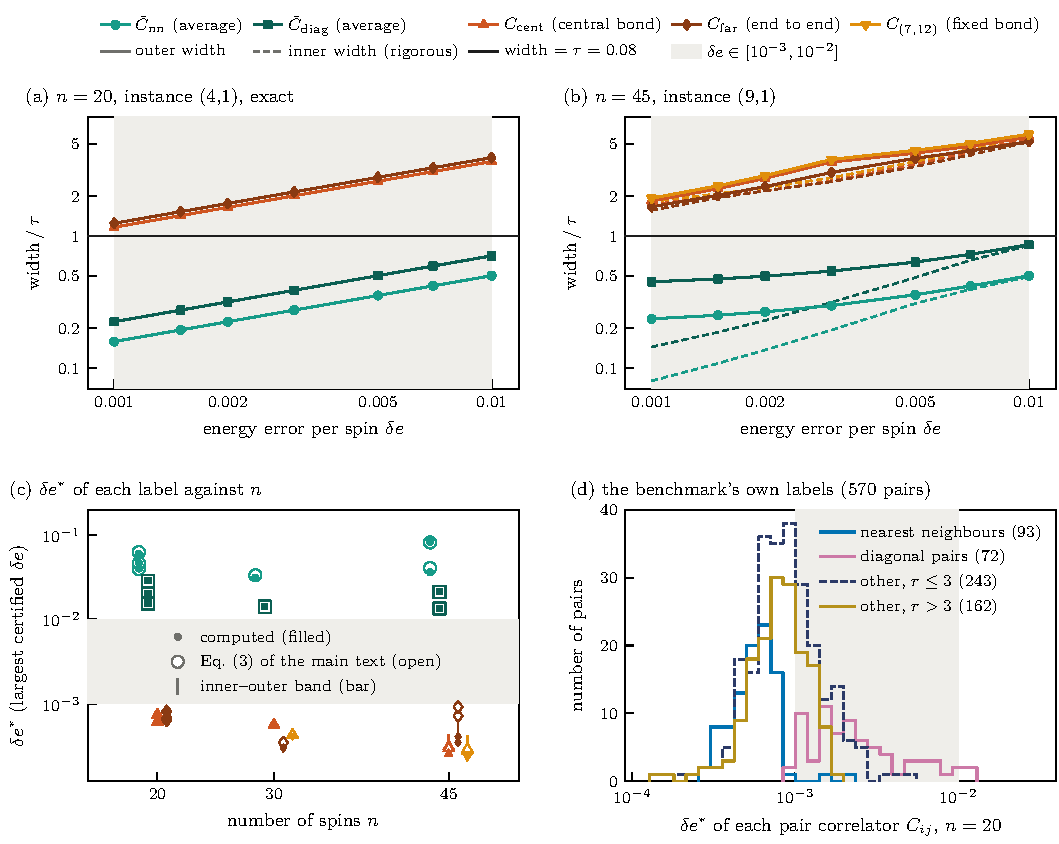
\includegraphics[width=\textwidth]{figS_huang_pgf}%
\caption{\label{fig:huang}The rule on the second benchmark~\cite{huang2022}. (a) Two-sided width over $\tau$ against the % src: file:phase3/full_runs/huang/RESULTS.md; def:phase3/full_runs/huang/DECLARATION.md
error per spin, $n=20$, instance $(4,1)$ (exact). (b) The same at $n=45$, instance $(9,1)$ (solid: outer, % src: file:phase3/full_runs/huang/RESULTS.md; def:phase3/full_runs/huang/DECLARATION.md
DMRG-referenced; dashed: inner, rigorous). (c) $\des$ of each label against $n$ (filled: computed; bars: band between
the inner and outer values; open: the leading-order law of Corollary~1 of the main text). The single pairs fall with $n$; the averages do not. % src: file:phase3/full_runs/huang/RESULTS.md; def:phase3/full_runs/huang/DECLARATION.md
(d) $\des$ of all 570 pair correlators at $n=20$ by class. Shaded: $\de\in[10^{-3},10^{-2}]$. Source: deposited % src: file:phase3/full_runs/huang/RESULTS.md; def:phase3/full_runs/huang/DECLARATION.md
outputs of the benchmark run.}
\end{figure}

\def\SMcap{The rule on the second benchmark. Each block is one label, each row one instance $(L,k)$. $\des_{\rm in}$:
the error per spin at which the rigorous inner width reaches $\tau$; $\des_{\rm out}$: the same for the outer width (equal
at $n=20$; a DMRG-referenced band at $n=30$, $45$); $\des_{\rm law}=S\tau^2/(8\chi n)$ with $\chi$ from the two % src: file:phase3/full_runs/huang/RESULTS.md; def:phase3/full_runs/huang/DECLARATION.md
smallest-field points; status at the seven grid values: C certified, N not certified (no gray rows).}\def\SMlab{tab:huang_featured}
\LTclearhead
% generated by figures/make_sm_new.py from phase3/full_runs/huang/laptop_analysis/summary_huang.json (rows[*].tau) -- do not edit
{\footnotesize\setlength{\tabcolsep}{5pt}\renewcommand{\arraystretch}{1.3}
\needspace{360pt}
\begin{longtable}{@{}lclccccl@{}}
\caption{\SMcap}\label{\SMlab}\\
\toprule
instance & $n$ & method & $\delta e^*_{\rm in}$ & $\delta e^*_{\rm out}$ & $\delta e^*_{\rm law}$ & law/out & status at $\delta e=10^{-3}\dots10^{-2}$ \\
\midrule
\multicolumn{8}{@{}l}{\textbf{$\bar C_{\rm nn}$ (average)}}\\
$(4,1)$ & 20 & exact & 0.040 & 0.040 & 0.040 & 0.988 & \texttt{C C C C C C C} \\
$(4,2)$ & 20 & exact & 0.047 & 0.047 & 0.046 & 0.994 & \texttt{C C C C C C C} \\
$(4,3)$ & 20 & exact & 0.060 & 0.060 & 0.063 & 1.05 & \texttt{C C C C C C C} \\
$(6,1)$ & 30 & DMRG & 0.032 & 0.031 & 0.033 & 1.07 & \texttt{C C C C C C C} \\
$(9,1)$ & 45 & DMRG & 0.036 & 0.036 & 0.041 & 1.12 & \texttt{C C C C C C C} \\
$(9,2)$ & 45 & DMRG & 0.085 & 0.083 & 0.082 & 0.981 & \texttt{C C C C C C C} \\
\multicolumn{8}{@{}l}{\textbf{$\bar C_{\rm diag}$ (average)}}\\
$(4,1)$ & 20 & exact & 0.020 & 0.020 & 0.020 & 0.995 & \texttt{C C C C C C C} \\
$(4,2)$ & 20 & exact & 0.016 & 0.016 & 0.015 & 0.991 & \texttt{C C C C C C C} \\
$(4,3)$ & 20 & exact & 0.029 & 0.029 & 0.029 & 0.995 & \texttt{C C C C C C C} \\
$(6,1)$ & 30 & DMRG & 0.014 & 0.014 & 0.014 & 0.999 & \texttt{C C C C C C C} \\
$(9,1)$ & 45 & DMRG & 0.014 & 0.014 & 0.013 & 0.996 & \texttt{C C C C C C C} \\
$(9,2)$ & 45 & DMRG & 0.022 & 0.021 & 0.021 & 0.987 & \texttt{C C C C C C C} \\
\multicolumn{8}{@{}l}{\textbf{$\bar C_{\rm stag}$ (average)}}\\
$(4,1)$ & 20 & exact & 0.010 & 0.010 & 0.010 & 1.00 & \texttt{C C C C C C C} \\
$(4,2)$ & 20 & exact & 0.012 & 0.012 & 0.012 & 1.00 & \texttt{C C C C C C C} \\
$(4,3)$ & 20 & exact & 0.015 & 0.015 & 0.015 & 0.988 & \texttt{C C C C C C C} \\
\bottomrule
\multicolumn{8}{r@{}}{\textit{continued on next page}}\\
\end{longtable}
\needspace{250pt}
\begin{center}\begin{tabular}{@{}lclccccl@{}}
\multicolumn{8}{@{}l}{\textit{Table \thetable\ (continued)}}\\
\toprule
instance & $n$ & method & $\delta e^*_{\rm in}$ & $\delta e^*_{\rm out}$ & $\delta e^*_{\rm law}$ & law/out & status at $\delta e=10^{-3}\dots10^{-2}$ \\
\midrule
\multicolumn{8}{@{}l}{\textbf{$C_{\rm cent}$ (central bond)}}\\
$(4,1)$ & 20 & exact & $7.3\times10^{-4}$ & $7.3\times10^{-4}$ & $7.3\times10^{-4}$ & 0.999 & \texttt{N N N N N N N} \\
$(4,2)$ & 20 & exact & $6.0\times10^{-4}$ & $6.0\times10^{-4}$ & $6.0\times10^{-4}$ & 0.999 & \texttt{N N N N N N N} \\
$(4,3)$ & 20 & exact & $7.4\times10^{-4}$ & $7.4\times10^{-4}$ & $7.4\times10^{-4}$ & 0.999 & \texttt{N N N N N N N} \\
$(6,1)$ & 30 & DMRG & $5.9\times10^{-4}$ & $5.5\times10^{-4}$ & $5.6\times10^{-4}$ & 1.02 & \texttt{N N N N N N N} \\
$(9,1)$ & 45 & DMRG & $3.7\times10^{-4}$ & $2.6\times10^{-4}$ & $3.1\times10^{-4}$ & 1.18 & \texttt{N N N N N N N} \\
$(9,2)$ & 45 & DMRG & $4.3\times10^{-4}$ & $2.5\times10^{-4}$ & $3.0\times10^{-4}$ & 1.17 & \texttt{N N N N N N N} \\
\multicolumn{8}{@{}l}{\textbf{$C_{(7,12)}$ (same bond, growing lattice)}}\\
$(6,1)$ & 30 & DMRG & $4.6\times10^{-4}$ & $4.2\times10^{-4}$ & $4.3\times10^{-4}$ & 1.03 & \texttt{N N N N N N N} \\
$(9,1)$ & 45 & DMRG & $3.4\times10^{-4}$ & $2.3\times10^{-4}$ & $2.8\times10^{-4}$ & 1.20 & \texttt{N N N N N N N} \\
$(9,2)$ & 45 & DMRG & $4.2\times10^{-4}$ & $2.4\times10^{-4}$ & $2.9\times10^{-4}$ & 1.18 & \texttt{N N N N N N N} \\
\multicolumn{8}{@{}l}{\textbf{$C_{\rm far}$ (end to end)}}\\
$(4,1)$ & 20 & exact & $6.4\times10^{-4}$ & $6.4\times10^{-4}$ & $6.4\times10^{-4}$ & 0.999 & \texttt{N N N N N N N} \\
$(4,2)$ & 20 & exact & $6.8\times10^{-4}$ & $6.7\times10^{-4}$ & $6.7\times10^{-4}$ & 0.999 & \texttt{N N N N N N N} \\
$(4,3)$ & 20 & exact & $8.1\times10^{-4}$ & $8.1\times10^{-4}$ & $8.1\times10^{-4}$ & 0.999 & \texttt{N N N N N N N} \\
$(6,1)$ & 30 & DMRG & $3.4\times10^{-4}$ & $3.0\times10^{-4}$ & $3.4\times10^{-4}$ & 1.16 & \texttt{N N N N N N N} \\
$(9,1)$ & 45 & DMRG & $4.6\times10^{-4}$ & $3.5\times10^{-4}$ & $7.2\times10^{-4}$ & 2.07 & \texttt{N N N N N N N} \\
$(9,2)$ & 45 & DMRG & $5.8\times10^{-4}$ & $4.1\times10^{-4}$ & $9.2\times10^{-4}$ & 2.25 & \texttt{N N N N N N N} \\
\bottomrule
\end{tabular}\end{center}
}


\def\SMcap{The benchmark's own labels: number of the 190 pair correlators of each $n=20$ instance certified (width $\le\tau=0.08$) % src: file:phase3/full_runs/huang/RESULTS.md; def:phase3/full_runs/huang/DECLARATION.md
at each error per spin (exact; the others are not certified).}\def\SMlab{tab:huang_pairs}
\LTclearhead
% generated by figures/make_sm_new.py from phase3/full_runs/huang/laptop_analysis/summary_huang.json (pairs[*][*].tau.status) -- do not edit
{\footnotesize\setlength{\tabcolsep}{5pt}\renewcommand{\arraystretch}{1.3}
\needspace{178pt}
\begin{longtable}{@{}lccccccc@{}}
\caption{\SMcap}\label{\SMlab}\\
\toprule
instance & $1.0\times10^{-3}$ & $1.5\times10^{-3}$ & $2.0\times10^{-3}$ & $3.0\times10^{-3}$ & $5.0\times10^{-3}$ & $7.0\times10^{-3}$ & $1.0\times10^{-2}$ \\
\midrule
$(4,1)$ & 56 & 23 & 15 & 9 & 6 & 4 & 1 \\
$(4,2)$ & 68 & 25 & 15 & 5 & 1 & 0 & 0 \\
$(4,3)$ & 82 & 45 & 24 & 10 & 5 & 3 & 2 \\
all (570 pairs) & 206 & 93 & 54 & 24 & 12 & 7 & 3 \\
\bottomrule
\end{longtable}
}



\emph{Outcomes of the predictions written down in advance.} (i) No $n=20$ pair certified at $\de=10^{-3}$: % src: file:phase3/full_runs/huang/RESULTS.md; def:phase3/full_runs/huang/DECLARATION.md
\emph{failed}. 206 of 570 pairs are certified there (70 of 72 diagonal pairs, 2 of 93 nearest-neighbour bonds), and 3 % src: file:phase3/full_runs/huang/RESULTS.md; def:phase3/full_runs/huang/DECLARATION.md
at $10^{-2}$. The diagonal pairs respond least to their conjugate field. (ii) The three single pairs not certified at % src: file:phase3/full_runs/huang/RESULTS.md; def:phase3/full_runs/huang/DECLARATION.md
$n=30$, $45$: \emph{holds}, at every grid value (widths $1.3$--$1.8\,\tau$ at $10^{-3}$). (iii) $\bar C_{\rm nn}$ % src: file:phase3/full_runs/huang/RESULTS.md; def:phase3/full_runs/huang/DECLARATION.md
certified on all six instances: \emph{holds}, over the whole grid ($\des=0.031$--$0.083$); $\bar C_{\rm diag}$ too. % src: file:phase3/full_runs/huang/RESULTS.md; def:phase3/full_runs/huang/DECLARATION.md
(iv) The accuracy law within $[0.8,1.25]$: holds for the 12 average rows ($0.981$--$1.121$) and for all 570 pairs % src: file:phase3/full_runs/huang/RESULTS.md; def:phase3/full_runs/huang/DECLARATION.md
(558 within $1\%$); at $n=30$, $45$ the precision we required of the reference energies (error at most $2\%$ of the % src: file:phase3/full_runs/huang/RESULTS.md; def:phase3/full_runs/huang/DECLARATION.md
smallest local $\epsilon_\tau$) was not reached ($3.7$--$18\%$), nor was the second declared requirement, on the chain % src: file:phase3/full_runs/huang/RESULTS.md; def:phase3/full_runs/huang/DECLARATION.md
energies at the decisive point of the central bond ($8\%$ against $1\%$), so the law test of the single pairs there is % src: file:phase3/full_runs/huang/RESULTS.md (ratio 0.079 / 0.084, limit 0.01); derived: 0.079-0.084 is about 8 %, 0.01 is 1 %
\emph{undecided}; as computed, two rows (the end-to-end pair at $n=45$) lie at $2.07$ and $2.26$. Taking $\chi$ at the % src: file:phase3/full_runs/huang/RESULTS.md; def:phase3/full_runs/huang/DECLARATION.md
second chain points, where the label shift exceeds the numerical noise, puts the law inside the computed band in all
nine rows (a diagnosis made afterwards). (v-a) The same bond in a growing lattice: $\des$ falls from $7.3\times10^{-4}$ % src: file:phase3/full_runs/huang/RESULTS.md; def:phase3/full_runs/huang/DECLARATION.md
($n=20$) to $4.2$--$4.6\times10^{-4}$ ($30$) and $2.3$--$3.4\times10^{-4}$ ($45$) while the energy needed to move it % src: file:phase3/full_runs/huang/RESULTS.md; def:phase3/full_runs/huang/DECLARATION.md
stays $0.010$--$0.019$: the $1/n$ of Corollary~1 of the main text (holds on the declared values, but formally undecided for the same % src: file:phase3/full_runs/huang/RESULTS.md; def:phase3/full_runs/huang/DECLARATION.md
precision reason). (v-b) $\des$ of $\bar C_{\rm nn}$ nearly the same at every size: \emph{failed} ($0.64$, $0.74$, % src: file:phase3/full_runs/huang/RESULTS.md; def:phase3/full_runs/huang/DECLARATION.md
$1.70$ times the $n=20$ mean); the spread between instances at fixed $n$ is larger than any size trend, and there is no % src: file:phase3/full_runs/huang/RESULTS.md; def:phase3/full_runs/huang/DECLARATION.md
$1/n$ decay. Checks: DMRG against exact diagonalization at $n=20$ ($\epsilon_\tau$ within $0.25\%$), 268 stored states % src: file:phase3/full_runs/huang/RESULTS.md; def:phase3/full_runs/huang/DECLARATION.md
in the sector, and 185 headline components re-evaluated in a separate process ($|\Delta E|\le1.2\times10^{-12}$). % src: file:phase3/full_runs/huang/RESULTS.md; def:phase3/full_runs/huang/DECLARATION.md

\section{Relation to prior work, item by item}
\label{sm:prior}

What each closest work proves and how the statements of the main text relate to it:
\begin{itemize}
\item \textbf{Jaderberg et al.~\cite{jaderberg2026}, with its public record~\cite{jaderberg2026data}.} \emph{Shows:} ground-state observables of the heavy-hex XXZ model at $57$ and $115$ qubits generated on a processor by sample-based Krylov diagonalization with a final basis optimization, a model trained on them and tested outside its training range, an Eckart-type bound that, as the paper notes, does not control local observables, and errors of its labels against its own DMRG reference. The paper states that its data are available on request; the labels, the energy of each sample and the DMRG values are public at $50$ couplings per size in a repository of one of its authors that names the paper, together with code that we read and did not run (Sec.~\ref{sm:public}; the block of the last step, Sec.~\ref{sm:bo}). \emph{Relation:} the dataset of the main text. We add what its published energy and site magnetizations certify about each label (Secs.~\ref{sm:map} and~\ref{sm:public}), the sign and trend of the label errors measured against the authors' reference (Sec.~\ref{sm:publictests}), and what a learner trained on the labels can guarantee (Sec.~\ref{sm:publiclearn}). % src: def:phase3/full_runs/real_data/DECLARATION.md (n = 57, 115; k = 11..60: 50 couplings)
\item \textbf{Eckart~\cite{eckart1930}.} \emph{Proves:} infidelity $\le\epsilon/\Delta$, so a local error $\lesssim\|O\|\sqrt{\epsilon/\Delta}$. \emph{Relation:} an upper bound, vacuous for $\epsilon\ge\Delta$; ours are lower bounds and hold in the extensive regime. % src: file:phase3/STEP0_witness_prior_art_feasibility.md
\item \textbf{Weinhold~\cite{weinhold1968}.} \emph{Proves:} bounds on expectation values from overlap information. \emph{Relation:} needs overlap or variance data, not energy only. % src: file:phase3/STEP0_witness_prior_art_feasibility.md
\item \textbf{Cohen and Feldmann~\cite{cohen1971}.} \emph{Proves:} Lagrange-multiplier bounds. \emph{Relation:} Lemma~A is theirs; the form with two constraints used for the public data adds a multiplier of the mean magnetization (Sec.~\ref{sm:proofs}). % src: file:phase3/STEP0_witness_prior_art_feasibility.md
\item \textbf{Manchanda~\cite{manchanda2026}, Thm.~1, Eq.~10, Cor.~1.} \emph{Proves:} radius $\le$ population $\epsilon\|H_{\rm ex}^{-1/2}O_{\rm ex}H_{\rm ex}^{-1/2}\|$ + coherence $\sqrt{2\epsilon\chi(\epsilon)}$, capped. \emph{Relation:} for an average at fixed $\de$ the population term grows with $n$ until the trivial cap; Theorem~2(b,c) replaces it by $\sqrt{2\chi_+\de}$, uniform in $n$. % src: file:phase3/STEP0_witness_prior_art_feasibility.md
\item \textbf{Manchanda, Thm.~2, Cor.~2.} \emph{Proves:} $\sqrt{2\epsilon\chi_O}\sqrt{1-\epsilon/\bar\Delta_O}\le$ radius for $\epsilon\le\bar\Delta_O/2$, with the exact ground state. \emph{Relation:} the small-$\epsilon$ case of Theorem~2 ($\chi_{\bar O}=\chi/n$ gives $\sqrt{2\de\chi}$); ours holds for all $\epsilon$ up to $O(n)$ with computable witnesses. % src: file:phase3/STEP0_witness_prior_art_feasibility.md
\item \textbf{Manchanda, Eq.~22.} \emph{Proves:} $\epsilon\lesssim\delta^2/(2\chi_O)$ at leading order. \emph{Relation:} Corollary~1 gives the exact form and the local and critical cases. % src: file:phase3/STEP0_witness_prior_art_feasibility.md
\item \textbf{Manchanda, discussion.} \emph{States:} that an algorithm and a system undergo certification failure when $\epsilon/\Delta$ diverges with the size, unless the transition elements vanish fast enough for the radius to stay finite (his footnote~3). \emph{Relation:} an average under the hypotheses of Theorem~2 is that excluded case, since $\chi_{\bar O}=\chi/n$, and the size-independent law holds for it; the statement stands for local labels and for order that no sector and no boundary pins (Theorem~3; Proposition~\ref{prop:unpinned}). % (structural: footnote and theorem numbers)
\item \textbf{Manchanda, Eqs.~17--19.} \emph{Proves:} symmetry selection rules, in-sector gap. \emph{Relation:} consistent with Theorem~2(d). % src: file:phase3/STEP0_witness_prior_art_feasibility.md; derived: theorem numbers
\item \textbf{Manchanda, applications.} \emph{Shows:} for the variational quantum eigensolver, DMRG and Krylov quantum diagonalization (lithium fluoride), that a well-converged energy can leave observables uncertified, with numerical evaluations of the exact region on systems of up to $20$ orbitals or $12$ spins. \emph{Relation:} the closest prior application; Krylov diagonalization is the algorithm family of the dataset of the main text. Every public label certified on that dataset has a published energy error of at most $0.05$ of the in-sector gap where that gap is stored ($0.07$ with the certificates added after the declaration), inside his regime $\epsilon\le\bar\Delta_O/2$; what is ours is uniformity in $n$ (a theorem at strong anisotropy, Sec.~\ref{sm:thm4}), the iff criterion of Theorem~3, intervals of a public dataset's own labels at $n=57$ and $115$ in exact arithmetic, and the method-class analysis. % src: map:row(115,4.0,m_s).eps_over_gap_in; derived: maximum 0.0427, at n = 115 and Jz = 4.0, of eps_pub times eps_over_gap_in over eps_dig, taken over the certified rows of the stored map, rounded up to 0.05; map:row(115,3.6,m_s).eps_over_gap_in; derived: maximum 0.0655 with the added certificates, rounded up to 0.07; derived: theorem numbers; file:phase3/STEP0_witness_prior_art_feasibility.md
\item \textbf{Wang et al.~\cite{wang2024prx,wang2026scipost}; Vall\'ee et al.~\cite{vallee2026}.} \emph{Proves:} window semidefinite bounds on any observable. \emph{Relation:} energy-only certificates, bounded below by $w_O$. % src: file:phase3/STEP0_witness_prior_art_feasibility.md
\item \textbf{Scheer et al.~\cite{scheer2025}.} \emph{Shows:} that thermodynamic-limit bootstrap bounds built on a ground-state positivity condition are loose in symmetry-broken phases, traces this by a heuristic argument to order-parameter defects that local operators cannot remove, and proves that bounds computed in an auxiliary model with ancilla spins hold for the original model; in its examples these are tighter. \emph{Relation:} not an energy-only certificate, since it adds a ground-state condition. The looseness has a related origin, low-energy states that differ in the order parameter; Theorem~3 gives the finite-$n$ energy-window statement with explicit thresholds. % (structural: theorem number)
\item \textbf{Banerjee et al.~\cite{banerjee2026}.} \emph{Proves:} rigorous two-sided bootstrap bounds on string order parameters once the ground-state energy is pinned within a window, with a sharpness set by the operators that enter the calculation. \emph{Relation:} an energy-window certificate built from positivity, bounded below by $w_O$. % src: file:phase3/STEP0_witness_prior_art_feasibility.md
\item \textbf{Ara\'ujo et al.~\cite{araujo2023}.} \emph{Proves:} ground-state optimality conditions. \emph{Relation:} not an energy-only certificate; our witnesses are not eigenstates. % src: file:phase3/STEP0_witness_prior_art_feasibility.md
\item \textbf{Wang et al.~\cite{wang2024prx,wang2026scipost}, as certificates.} \emph{Proves:} certified bounds on ground-state observables from semidefinite relaxations combined with variational energies~\cite{wang2024prx}, up to $16\times16$ lattices~\cite{wang2026scipost}; Ref.~\cite{wang2024prx} notes that such bounds can use energies ``obtained using variational quantum hardware or simulators'' and lists among natural continuations to ``validate the output of existing quantum simulators on specific finite-size instances of quantum many-body problems''. \emph{Relation:} the certificate side of Sec.~\ref{sm:rigor} uses the same principle, with a local-consistency relaxation in Lagrangian form at a fixed energy and, for the public data, a fixed mean magnetization; here the simulator outputs validated are the labels of a public dataset. Relaxations had earlier verified the energies of a quantum annealer on classical spin problems~\cite{baccari2020}, and sample-based methods suit this programme, since their stored wavefunctions permit ``a classical prover to certify them''~\cite{robledo2025}. % src: file:phase3/STEP0_witness_prior_art_feasibility.md
\item \textbf{Lin et al.~\cite{lin2026}; Anderson~\cite{anderson1951}; Barthel and H\"ubener~\cite{barthel2012}; Baumgratz and Plenio~\cite{baumgratz2012}.} \emph{Proves:} local relaxation hierarchies for ground energies: a first level that imposes consistency of pairwise reduced density matrices, relaxations over a family of clusters whose marginals agree on the overlaps, and message-passing solvers of their duals, one of them with a smoothed objective~\cite{lin2026}; the cluster lower bound that these relaxations generalize~\cite{anderson1951}; lower bounds on ground energies from semidefinite relaxations of another kind, with positivity of moment matrices: of few-particle Green's functions, with constraint operators supported on subsets of the lattice~\cite{barthel2012}, and of the one- and two-particle reduced density matrices of the whole system~\cite{baumgratz2012}. \emph{Relation:} our relaxation is of the cluster-family kind of Ref.~\cite{lin2026}, with clusters of five to nine sites (in dual form an optimized Anderson bound) and one more constraint, the mean magnetization, whose multiplier enters the bound; it is solved, as there, through a smoothed dual. We add that multiplier, the exact verification and the use for labels. % src: file:phase3/STEP0_witness_prior_art_feasibility.md
\item \textbf{Naceur et al.~\cite{naceur2025}.} \emph{Proves:} rigorous bounds from inexact numerical solutions by rational post-processing. \emph{Relation:} the same idea, applied to the cluster dual with integer elimination. % src: file:phase3/STEP0_witness_prior_art_feasibility.md
\item \textbf{Nachtergaele, Sims and Young~\cite{nsy2022}.} \emph{Proves:} that the spectral gap of a frustration-free model is stable, uniformly in the volume, under the perturbations of their uniform perturbation models (their Theorem~6.8). \emph{Relation:} the proof of Theorem~4 of the main text verifies their hypotheses for the dataset's model on the open heavy-hex patches at strong anisotropy (Sec.~\ref{sm:thm4}); ours are the site-by-site classical bound on the patches at every size, the verification with an open boundary, and the reading in terms of the window. The threshold coupling that follows is not explicit. % (structural: theorem numbers)
\item \textbf{Nachtergaele and Sims~\cite{nachtergaele2006}; Hastings and Koma~\cite{hastings2006}.} \emph{Proves:} exponential clustering of ground-state correlations from a spectral gap and Lieb--Robinson bounds; Ref.~\cite{nachtergaele2006} in a form that applies to finite systems as it stands, with explicit constants. \emph{Relation:} gives the constant $C_1$ of Theorem~2(c) from the gap; Lemma~\ref{lem:field}(d) notes that the proof uses the gap only for the states that the observable creates from the ground state, so that for labels that commute with the conserved charge the gap inside the sector suffices. % (structural: theorem numbers)
\item \textbf{Yarotsky~\cite{yarotsky2006}.} \emph{Proves:} a unique gapped ground state for relatively bounded quantum perturbations of classical lattice systems, on cubic volumes (his Theorem~1). \emph{Relation:} a second route to the uniform gap of Theorem~4 on the periodic lattices (Sec.~\ref{sm:thm4}), with a ten-site cell; we compared our setting with the statement of his theorem and did not re-derive his proof, and Theorem~4 does not depend on this route. % (structural: theorem numbers)
\item \textbf{Horsch and von der Linden~\cite{horsch1988}; Koma and Tasaki~\cite{koma1994}.} \emph{Proves:} in a ground state with long-range order that nothing pins, the order-parameter operator creates a state whose energy lies within order $1/n$ of the ground energy; Ref.~\cite{koma1994} gives the general form (their Theorem~2.2). The article of Ref.~\cite{horsch1988} was not read; we use its theorem in the form of Ref.~\cite{koma1994}, Sec.~2.2. \emph{Relation:} Proposition~\ref{prop:unpinned} is that theorem read in terms of the window: beyond a size $n\ge\sqrt{K/(4m_0^2\de)}$ the energy cannot certify an order parameter that no sector and no boundary pins. The heavy-hex sectors of the dataset pin the orientation, so this class is not the dataset's. % (structural: theorem numbers and a formula)
\item \textbf{Huang et al.~\cite{huang2022}.} \emph{Proves:} provable learning of ground-state properties; provides the benchmark of Sec.~\ref{sm:huang}. \emph{Relation:} our rule says which of its labels the energy certifies.
\item \textbf{Javanmardi et al.~\cite{javanmardi2023}; Cauchois et al.~\cite{cauchois2022}; Einbinder et al.~\cite{einbinder2022}.} \emph{Proves:} validity of conformal prediction with set-valued labels when each calibration score is replaced by its greatest value over the label's set~\cite{javanmardi2023}; lower bounds on the size of any prediction set that covers the true label, without assumptions on the distribution, from weak labels~\cite{cauchois2022}; validity of standard calibration for the true label when the label noise only adds dispersion, with examples in which a systematic error defeats it~\cite{einbinder2022}. \emph{Relation:} Proposition~2(b) is the score of Ref.~\cite{javanmardi2023} with the set supplied by the energy of each label; its part (d) and the remark of Sec.~\ref{sm:prop2proofs} make the price in width explicit for energy intervals; the public labels are a case of systematic error (Sec.~\ref{sm:publiclearn}). % (structural: proposition number)
\item \textbf{Gaberle and Jattana~\cite{gaberle2026}.} \emph{Shows:} in exact calculations of up to $20$ qubits, subspaces built from configurations of exact ground states, among them those of the most probable configurations, need a number of configurations that grows exponentially with size. \emph{Relation:} the same perfect-sample and most-probable-subset diagnostics as Sec.~\ref{sm:emu}, there for the energy, here for the sign of the label error. % (structural: sizes in the cited work)
\item \textbf{Biswas et al.~\cite{biswas2025}.} \emph{Shows:} an energy-error bound by the captured weight, and spin correlations reproduced across regimes, against exact diagonalization at $24$ sites, for a symmetry-filtered sampled-subspace method. \emph{Relation:} a counterpoint for a related method at a smaller size; for the Krylov variant near the isotropic point our emulation finds a one-signed label bias, and the public labels of the dataset show the same sign (Sec.~\ref{sm:publictests}). % (structural: sizes in the cited work)
\item \textbf{Candelori et al.~\cite{candelori2026}.} \emph{Shows:} the Krylov method of the dataset, sample-based Krylov quantum diagonalization run on a processor, computing the low-energy states of data Hamiltonians inside a supervised learner of classical data. \emph{Relation:} a further use of the algorithm family of the dataset of the main text, in which the outputs of the method are not training labels of ground states.
\item \textbf{Our earlier work~\cite{bonilla2026review,bonilla2026spectral}.} \emph{Shows:} a review that proposed a benchmarking standard against classical selectors for sample-based diagonalization~\cite{bonilla2026review}, and a proof that no error bound on a spectral function indexed on the captured weight alone beats the trivial one~\cite{bonilla2026spectral}. \emph{Relation:} the same kind of question put to other diagnostics of sample-based diagonalization; here the diagnostic under test is the energy.
\item \textbf{Koridon et al.~\cite{koridon2024}.} \emph{Shows:} a model trained on data with the expressibility and optimization errors of the variational quantum eigensolver replicates those biases. \emph{Relation:} the learning message of Corollary~2, shown there in practice and here on public processor labels (Sec.~\ref{sm:publiclearn}). % (structural: corollary number)
\item \textbf{Chen~\cite{chen2026}; Niu et al.~\cite{niu2026}.} \emph{Show:} the sector-projected energy does not certify that a prepared state lies in its sector; energy accuracy alone hides differences between prepared states. \emph{Relation:} the former bears on the sector constraint of the theory: the published states of the dataset are not in the sector (Sec.~\ref{sm:public}), which is why their labels are certified in a window of energy and mean magnetization; what a missing constraint costs is checked exactly in Sec.~\ref{sm:checks}, T7. % src: file:phase3/STEP0_witness_prior_art_feasibility.md
\end{itemize}

\section{Provenance: re-executed, only compared, not checked}
\label{sm:prov}

\emph{Computed for this paper before the public data were used.} The figures-based map: 358 DMRG tasks at $n=19$, $57$ and $115$ (references, chains with 2680 stored % src: file:phase3/full_runs/map/RESULTS.md
sector states, consistency checks, minimal bond dimension), the exact diagonalization at $n=19$, and the % src: file:phase3/full_runs/map/RESULTS.md; def:phase3/full_runs/map/DECLARATION.md; file:phase3/full_runs/method/RESULTS.md; file:phase3/full_runs/method/laptop_post/results_tables.md; def:phase3/full_runs/method/DECLARATION.md; file:phase3/full_runs/rigor/RESULTS_v2.md; file:phase3/full_runs/rigor/RESULTS.md; file:phase3/full_runs/huang/RESULTS.md
separate-process re-evaluation of 508 headline components. The rigorous bounds: 55 certificates in the earlier test and % src: file:phase3/full_runs/map/RESULTS.md; def:phase3/full_runs/map/DECLARATION.md; file:phase3/full_runs/method/RESULTS.md; file:phase3/full_runs/method/laptop_post/results_tables.md; def:phase3/full_runs/method/DECLARATION.md; file:phase3/full_runs/rigor/RESULTS_v2.md; file:phase3/full_runs/rigor/RESULTS.md; file:phase3/full_runs/huang/RESULTS.md
135 in the grid run, each verified exactly in a separate process, with 42 exact diagonalizations at $n=19$. The % src: file:phase3/full_runs/map/RESULTS.md; def:phase3/full_runs/map/DECLARATION.md; file:phase3/full_runs/method/RESULTS.md; file:phase3/full_runs/method/laptop_post/results_tables.md; def:phase3/full_runs/method/DECLARATION.md; file:phase3/full_runs/rigor/RESULTS_v2.md; file:phase3/full_runs/rigor/RESULTS.md; file:phase3/full_runs/huang/RESULTS.md
emulation: 100 tasks (references, Krylov runs, calibrations, emulations, perfect-sampler scans, basis optimization, % src: file:phase3/full_runs/method/RESULTS.md
``$+$'' chains), with 14 earlier $n=57$ Krylov sample sets reused after verification of their checksums. Our device % src: file:phase3/full_runs/map/RESULTS.md; def:phase3/full_runs/map/DECLARATION.md; file:phase3/full_runs/method/RESULTS.md; file:phase3/full_runs/method/laptop_post/results_tables.md; def:phase3/full_runs/method/DECLARATION.md; file:phase3/full_runs/rigor/RESULTS_v2.md; file:phase3/full_runs/rigor/RESULTS.md; file:phase3/full_runs/huang/RESULTS.md
data: two device jobs (Sec.~\ref{sm:qpu}) and their noiseless control, and the declared job at $\Jz=6.0$ % src: file:phase3/full_runs/final_tests/RESULTS.md (6.0)
(Sec.~\ref{sec:declared}). The second benchmark: 84 tasks (exact % src: file:phase3/full_runs/map/RESULTS.md; def:phase3/full_runs/map/DECLARATION.md; file:phase3/full_runs/method/RESULTS.md; file:phase3/full_runs/method/laptop_post/results_tables.md; def:phase3/full_runs/method/DECLARATION.md; file:phase3/full_runs/rigor/RESULTS_v2.md; file:phase3/full_runs/rigor/RESULTS.md; file:phase3/full_runs/huang/RESULTS.md
diagonalization at $n=20$, DMRG at $n=20$--$45$). On a laptop: the analyses from the fetched outputs, the two pure % src: file:phase3/full_runs/map/RESULTS.md; def:phase3/full_runs/map/DECLARATION.md; file:phase3/full_runs/method/RESULTS.md; file:phase3/full_runs/method/laptop_post/results_tables.md; def:phase3/full_runs/method/DECLARATION.md; file:phase3/full_runs/rigor/RESULTS_v2.md; file:phase3/full_runs/rigor/RESULTS.md; file:phase3/full_runs/huang/RESULTS.md
witnesses, both digitizations, the learning study on emulated labels, the exact checks of Sec.~\ref{sm:checks}, and
the figures and tables built on them. The exploratory bias analysis (Sec.~\ref{sec:biaslaw}): exact diagonalization at $n=19$ and a % src: file:phase3/full_runs/bias_law/code/bias_law.py (n = 19)
re-analysis of stored outputs, on a laptop. The declared tests (Sec.~\ref{sec:declared}): $128$ computing tasks on a % src: file:phase3/full_runs/final_tests/RESULTS.md (128)
virtual machine; for the job at $\Jz=6.0$, the exact Rayleigh quotient on the same virtual machine and the interval, in % src: file:phase3/full_runs/final_tests/RESULTS.md (6.0)
exact arithmetic, on a laptop.
The window test of Sec.~\ref{sm:window}: exact ground states and envelope chains at $n=24$, DMRG, % src: def:phase3/full_runs/kill_tests/W_window/DECLARATION.md (n = 24)
transformer networks and an idealized Krylov generator on a virtual machine, with the arithmetic of its comparison
with published states on a laptop. After the fifth independent reading of this paper, post-hoc checks that read stored outputs only: the margins
and $n=19$ comparisons of the figures-based map, the tolerance scan of $J^*$, and the costs and energy errors of
Sec.~\ref{sec:declared} (\texttt{final\_tests/code/post\_checks*.py}, \texttt{map/laptop\_analysis/code/tau\_scan.py},
whose $6\%$ run reproduces the stored map exactly). % src: def:phase3/full_runs/map/laptop_analysis/code/tau_scan.py (0.06)

\emph{Computed for this paper on the public data} (all on a laptop; Secs.~\ref{sm:public}, \ref{sm:publictests}
and~\ref{sm:publiclearn}). The public record was downloaded once, at a pinned commit, and converted to plain numbers
without running any of its code; a second run of the converter on its $302$ data files reproduced the converted % src: file:phase3/full_runs/real_data/checks/G1_rerun_2026-11-12.md (302 data members)
files byte for byte. The map: $700$ rows (seven labels at the $50$ couplings of each size), with exact intervals in % src: rdq:n_rows (700); rdp:sizes.57.n_couplings (50)
rational arithmetic from $140$ stored certificates and, on the other side, explicit states built from the stored % src: rdq:certificates.n_used (140)
DMRG states. The certificates added after the declaration: $48$, found in a search whose settings were fixed in % src: rdeq:certificates_E1 (48)
writing before it started, each accepted by two exact verifiers. The tests of the bias: sign, trend and curve at the
$50$ couplings of each size, with the curves from exact diagonalization at $n=19$ at the same couplings. The % src: rdp:sizes.57.n_couplings (50)
learning tests: standard prediction intervals (the plain jackknife) of a cubic model, of a nearest-neighbour null
and, in part after the primary results were known, of a small neural network, the floor for any
learner, and the constructive test in $200$ random splits of each set, with a secondary run of the same code on % src: rdl:summary.57.f3.sets.S_1_2.models.M1.n_splits (200)
the sets extended by the added certificates. An independent recomputation, with programs written separately that
import nothing from the analysis code, reproduced the main numbers of the map (every exact interval as a rational
number, also with the added certificates), of the tests of the bias, and of the floor and the constructive test
(Sec.~\ref{sm:public_audit}). In the eleventh reading of this paper, code written separately by a reader
reproduced every printed number of the secondary run and gave the post-hoc jackknife+ counts of % src: file:phase3/full_runs/real_data/checks/r11/fl_learn_recompute_e1_out.txt (200 of 200 splits; 15 of 200 splits); file:phase3/full_runs/real_data/checks/r11/fl_learn_paper_numbers_out.txt (41 labels and 0 truths of 45)
Sec.~VI~A of the main text; copies of these scripts and their outputs are kept with the analysis. The four
figures of the main text and the tables of the three sections named above
are generated from the stored outputs by scripts (\texttt{paper/figures/pgf\_*\_rd/} and
\texttt{paper/figures/sm\_tables/make\_rd*.py}).

\emph{Computed for the statements added to the theory} (Secs.~\ref{sm:proofs}, \ref{sm:checks} and~\ref{sm:thm4};
on a laptop). For Theorem~4: the geometry of the heavy-hex patches and their numbering, checked by computer for % (structural: theorem number)
every odd distance up to $41$, and exact diagonalization at $n=19$. For the field lemma, the contour bound, the two % src: file:paper/reviews/R10_2026-11-12/scratch/theory-theorem4/geometry_peierls_out.txt (d = 3..41: True)
propositions on sublinear classes and the floor of Proposition~2: exact diagonalization and enumeration on small % (structural: proposition number)
systems. Each statement was checked numerically by its writer and attacked by a referee with separate code, and
what the referees added was checked by a verifier who used none of the earlier code. The window of energy and mean
magnetization was computed exactly on a $12$-site comb. These scripts and their outputs go with the deposit. % src: file:paper/reviews/R10_2026-11-12/scratch/rw-T/t_mean_window_out.txt (n = 12)

\emph{Only compared.} The dataset paper's energy ratios, gaps, label errors and string counts, read from its figures
and text, against the public record (Sec.~\ref{sm:figmap}); the authors' DMRG values against our references where
both exist (Sec.~\ref{sm:public});
earlier pilot computations, which the figures-based map reproduces to $\le10^{-3}$ in every width; the benchmark's stored % src: file:phase3/full_runs/map/RESULTS.md; def:phase3/full_runs/map/DECLARATION.md; file:phase3/full_runs/method/RESULTS.md; file:phase3/full_runs/method/laptop_post/results_tables.md; def:phase3/full_runs/method/DECLARATION.md; file:phase3/full_runs/rigor/RESULTS_v2.md; file:phase3/full_runs/rigor/RESULTS.md; file:phase3/full_runs/huang/RESULTS.md
correlators and energies; the published variational energies and moments and the Monte Carlo constants of
Sec.~\ref{sm:window}. Of the published theorems that the new statements use
(Refs.~\cite{nsy2022,nachtergaele2006,koma1994,yarotsky2006} for the theory and
Refs.~\cite{javanmardi2023,cauchois2022,einbinder2022} for Proposition~2), the statements were read and their % (structural: proposition number)
hypotheses compared with our setting; their proofs were not re-derived, except that of the clustering theorem of
Ref.~\cite{nachtergaele2006}, which was followed step by step for Lemma~\ref{lem:field}(d).

\emph{Outcomes, listed together.} Outcomes are reported with the same prominence whether or not they meet the plan;
the main text gives each where it occurs. Of the computations declared before the public data were used: the
emulation at $n=115$ missed its declared energy condition; the accuracy law of the figures-based map left its band % src: def:phase3/full_runs/method/DECLARATION.md (n = 115)
at six rows; one rigorous block was rejected; two benchmark predictions failed and two were left undecided; the % src: map:claims.C-D.outside (6 rows)
realistic benchmark generator left coverage intact; the curve of the bias passed its declared test on new emulated
labels; the corrected labels failed the declared test on disordered lattices; and the declared device run was made
two days later than declared, and its label at $\Jz=6.0$ has an interval below the tolerance. On the public % src: file:phase3/full_runs/final_tests/RESULTS.md (6.0)
data: the curve failed its declared test, on its second condition at $n=115$ (its limit on the mean miss at % src: def:phase3/full_runs/real_data/DECLARATION.md (n = 115)
$n=115$ was already met by the uncorrected labels, so only the limit at $n=57$ tested anything); the constructive % src: def:phase3/full_runs/real_data/DECLARATION.md (n = 57, 115)
learning test failed on the full set of certified labels and on the set certified to three quarters of the
tolerance, and passed on the set certified to half of it; a claim fixed in advance for the figures-based map, that
no single-site or single-bond label is certified, does not hold like for like at the published energies, where two
such rows pass for sector states at $n=57$, $\Jz=6.0$ (in the window of energy and mean magnetization they are % src: def:phase3/full_runs/real_data/DECLARATION.md (n = 57)
undecided, since no certificate was computed for a local label); and one row inside the range of the certificates,
$\ms$ at $n=57$, $\Jz=3.4$, is not within the tolerance ($1.0043\,\tau$) and stays undecided. % src: file:phase3/full_runs/real_data/RESULTS.md (1.0043); rdam:C_six.57_3.4 (1.00424); derived: 1.00424 rounded up to 1.0043

\emph{Not checked, or not complete.} \emph{Hypothesis H}, that the published energy and the site magnetizations and
correlations of a sample are expectation values of one state: the public record does not contain the states, so it cannot be checked;
a necessary condition holds at all $100$ points (Sec.~\ref{sm:public}). \emph{The off-grid rule against the % src: file:phase3/full_runs/real_data/RESULTS.md (100 points)
tensors:} the declaration asks for the energy, recomputed from the tensors, of the $150$ states that decide $32$ % src: file:phase3/full_runs/real_data/RESULTS.md (32 rows selected; 150 components)
selected rows. This check was not completed: none of those tensors is on the machine on which the analysis ran, and
the archive that holds them was not opened. The six states whose tensors are available agree with the rule to
$1.6\times10^{-13}$. The rule is used by $280$ of the $439$ ``not certified'' rows and by the lower widths and the % src: file:phase3/full_runs/real_data/DEVIATIONS.md (1.6e-13); file:phase3/full_runs/real_data/RESULTS.md (280 of the 439 NOT CERTIFIED rows)
floor of the learning tests; the statements at the test couplings and at the grid couplings, and the whole
certified side, do not use it (Sec.~\ref{sm:public_checks}). \emph{The learning tests:} of the models declared, the
small neural network inside the training range at $n=57$ and at $n=115$ and the dataset paper's architecture~1 % (sizes; architecture number of the cited work)
(our implementation) at the test couplings of $n=57$ were not run by the declared analysis, for cost; they were run % (sizes)
afterwards, after the primary results were known, with the declared code unchanged, and decide nothing
(Sec.~\ref{sm:publiclearn}).
\emph{Times:} the checksum of the declaration of the analyses on the public data was computed on our own machine
and its time is that of our own files; there is no external time stamp. \emph{The theory:} the article of
Ref.~\cite{horsch1988} was not read, and its theorem is used as stated in Ref.~\cite{koma1994}; the lemma on single
sites in a sector and the bound on the weight of the reversed sector at a fixed mean magnetization
(Sec.~\ref{sm:proofs}) were verified by hand and on exact examples and have not been attacked with independent
code; the second route to Theorem~4 on the periodic lattices rests on a published theorem whose proof was not % (structural: theorem number)
re-derived. \emph{Not computed:} rigorous lower bounds for $\Ctwo$ and the local labels, and $\ms$ certificates at
couplings other than those of Sec.~\ref{sm:public}; bounds at $n=30$, $45$ of the % src: file:phase3/full_runs/map/RESULTS.md; def:phase3/full_runs/map/DECLARATION.md; file:phase3/full_runs/method/RESULTS.md; file:phase3/full_runs/method/laptop_post/results_tables.md; def:phase3/full_runs/method/DECLARATION.md; file:phase3/full_runs/rigor/RESULTS_v2.md; file:phase3/full_runs/rigor/RESULTS.md; file:phase3/full_runs/huang/RESULTS.md
benchmark; run-to-run variation on our device and of the public labels, of which the record holds one state per
coupling; DMRG beyond bond dimension $320$ at $n=115$. \emph{Not run:} the code of the public record, which was % src: file:phase3/full_runs/map/RESULTS.md; def:phase3/full_runs/map/DECLARATION.md; file:phase3/full_runs/method/RESULTS.md; file:phase3/full_runs/method/laptop_post/results_tables.md; def:phase3/full_runs/method/DECLARATION.md; file:phase3/full_runs/rigor/RESULTS_v2.md; file:phase3/full_runs/rigor/RESULTS.md; file:phase3/full_runs/huang/RESULTS.md
read as text: for hypothesis H, for the computation of the labels and of the stored energy (Sec.~\ref{sm:public})
and for the block of the last step (Sec.~\ref{sm:bo}). \emph{Not used:} the circuits and raw samples behind the
dataset.

\emph{Moved to the ancillary file} \texttt{tables.pdf} (generated by the same scripts from the same deposited
outputs): the full tables of the figures-based map (widths and status at $n=57$ and $115$, the accuracy law row by row), the % src: file:phase3/full_runs/map/RESULTS.md; def:phase3/full_runs/map/DECLARATION.md; file:phase3/full_runs/method/RESULTS.md; file:phase3/full_runs/method/laptop_post/results_tables.md; def:phase3/full_runs/method/DECLARATION.md; file:phase3/full_runs/rigor/RESULTS_v2.md; file:phase3/full_runs/rigor/RESULTS.md; file:phase3/full_runs/huang/RESULTS.md
perfect-sampling table, the window-position table, and the $n=115$ landscape and lattice figures. % src: file:phase3/full_runs/map/RESULTS.md; def:phase3/full_runs/map/DECLARATION.md; file:phase3/full_runs/method/RESULTS.md; file:phase3/full_runs/method/laptop_post/results_tables.md; def:phase3/full_runs/method/DECLARATION.md; file:phase3/full_runs/rigor/RESULTS_v2.md; file:phase3/full_runs/rigor/RESULTS.md; file:phase3/full_runs/huang/RESULTS.md

\section{Further material on the rule, the map, the method class and the benchmark}
\label{sm:moved}

This section collects remarks on the rule, the map in detail, the mechanism of the method class and the per-label
numbers of the benchmark. Unless a passage names the public data, its statements about the dataset of
Ref.~\cite{jaderberg2026} are properties of the model in its sector, of the emulated method class under stated
assumptions, or readings of the figures of that paper; the measurements on the public labels are in
Secs.~\ref{sm:public}, \ref{sm:publictests} and~\ref{sm:publiclearn}.

\subsection{Remarks on the rule}

\emph{Tightness of $N^*$ (Theorem~1 of the main text).} $N^*$ is the size from which the reset construction fills % (structural: theorem number)
the range, and the bound is attained for non-interacting spins and loose otherwise. In exact checks on the open
transverse-field Ising chain ($h=1.5$, $Z$ at the centre, $\kappa_A=7$), the window of $Z$ reaches $99\%$ of its range % src: file:paper/data/crosschecks/check2_output.txt (h=1.5; kappa_A = 7; 99%)
at $n=10$ for $\de=0.1$ ($N^*=70$) and at $n=6$ for $\de=0.2$ ($N^*=35$), i.e.\ about six to seven times earlier % src: file:paper/data/crosschecks/check2_output.txt (n = 10; 0.10; 70.0; n = 6; 0.20; 35.0)
than $N^*$; in a U(1) sector the bound of Theorem~1(b) gives $0.016$--$0.25$ where the extents actually reached are % src: file:paper/data/crosschecks/check2_output.txt (0.0159-0.2460); derived: 0.2460 rounded to 0.25
$0.59$--$1.00$ (Sec.~\ref{sm:checks}). The factor is a property of that chain at that field: it is $24$ at $h=0.8$ % src: file:paper/data/crosschecks/check2_output.txt (0.5876-1.0000); file:paper/reviews/R10_2026-11-12/scratch/math-thm1/t3_looseness_output.txt (h=0.8, 24.10); derived: rounded
and $2.9$ at $h=5.0$ (Sec.~\ref{sm:proofs}), so $N^*$ divided by a fixed number does not estimate where certification is lost. % src: file:paper/reviews/R10_2026-11-12/scratch/math-thm1/t3_looseness_output.txt (h=5.0, 2.86); derived: rounded
What matters for certification is the tolerance, not the full range: for the dataset's Hamiltonian at $\Jz=1.6$
and the published error per site there the bound gives $N^*\approx460$ for a single $Z_i$, but already excludes % src: rdm:rows[n=57,Jz=1.6,label=Z_bulk].de_real (0.011355); derived: 5.2/0.011355 = 458
certification at tolerance $\tau$ for $n\ge12$, and the stored states show that the bulk site stops being certified % src: derived: 0.046338 x 5.2/(1.79116 x 0.011355) = 11.85, as in the remark that follows the proof of Theorem 1
at an excess energy of $8.3$--$8.6\times10^{-4}$ at $n=57$ (Sec.~\ref{sm:proofs}). Explicit sector states of energy % src: map:row(57,1.6,Z_bulk).eps_tau_out (8.349e-4); map:row(57,1.6,Z_bulk).eps_tau_in (8.557e-4); derived: ends rounded outward
below the published one reach $50$--$62\%$ of the range of the four local labels at that coupling and size. % src: map:row(57,1.6,Czz_edge).at_lo.w_in (0.9925 of range 2); map:row(57,1.6,Z_boundary).at_lo.w_in (1.2345 of 2); derived: halves of the widths of the four local labels at Jz = 1.6, at an excess energy of 0.499, below the published 0.647

\emph{Averages above the gap, and where uniformity fails (Theorem~2 of the main text).} The gap enters only through % (structural: theorem number)
the deformed family's susceptibility, never through $\epsilon/\Delta$. In the exact checks the width of an
extensively pinned comb ferrimagnet stays intensive at $\epsilon/\Delta=2.14$ (width $1.2936$ at $n=12$ against % src: r3:t3_comb.txt (eps/gap 2.14, w 1.29360)
$1.2894$ at $n=6$), a regime where the lower bound of Ref.~\cite{manchanda2026} does not apply % src: r3:t3_comb.txt (1.28938)
[Fig.~\ref{figS:rule}(a)]. Part (c) of Theorem~2 is a sufficient condition, and on the side that opposes a pinned % (structural: theorem/corollary numbers)
order it can fail: there the deformed family can cross to a reversed-domain state at a field that decreases with
$n$. On the same comb, the deformed gap at $\mu=-0.4$ falls as $0.229$, $0.131$ and $0.087$ for $n=6$, $9$ and $12$, % src: file:paper/data/crosschecks/check3_output.txt (mu=-0.4; Delta* = 0.2288, 0.1307, 0.08689); derived: rounded to three digits
so the bound $2C_1/\Delta_*$ grows to $21$, $41$ and $65$ while $\chi_+$ itself stays near $1.5$ % src: file:paper/data/crosschecks/check3_output.txt (20.9967, 40.6295, 65.0814; chi+ = 1.5681, 1.5299, 1.4942); derived: rounded
(Sec.~\ref{sm:checks}); the same crossing makes the accuracy law fail for $\ms$ at $\Jz\ge5$ (Sec.~\ref{sm:moved_map}).
At finite $n$ it is an avoided crossing, since the sector ground state is non-degenerate (Sec.~\ref{sm:proofs}).
Three statements now limit where it can happen on the dataset's graphs: the classical part of the family cannot
cross for $|\mu|<\Jz/32$ at any size (Lemma~\ref{lem:peierls}); a uniform sector gap alone bounds $C_1$ % (formula)
(Lemma~\ref{lem:field}); and for $\Jz\ge J_c$ the gap is uniform on both sides (Theorem~4, Sec.~\ref{sm:thm4}), with % (structural: theorem number)
a $J_c$ that is not explicit and exceeds the lower part of the dataset's range.

\emph{Other classes.} Two classes with sublinear cost are now propositions of Sec.~\ref{sm:proofs}. An order
parameter that no sector and no boundary pins has $E^*_n\le K/(4nm_0^2)$ up to its long-range order
(Proposition~\ref{prop:unpinned}, after Horsch and von der Linden and Koma and Tasaki). An order whose orientation
is fixed only by a boundary or by a sector of bounded net charge pays at most the boundary terms of a region with a
sublattice-exchanging symmetry, $E^*\lesssim n^{(D-1)/D}$ in $D$ dimensions where such regions exist, a cost that
grows with $n$ but not linearly (Proposition~\ref{prop:wall}); on the heavy-hex patches no such region has a
sublinear boundary. The critical class remains heuristic: from a thermodynamic-limit argument that we do not prove,
at a critical point $E^*\sim nc^{1+\delta}$ and the width scales as $\de^{1/(1+\delta)}$.

\begin{figure}[h]
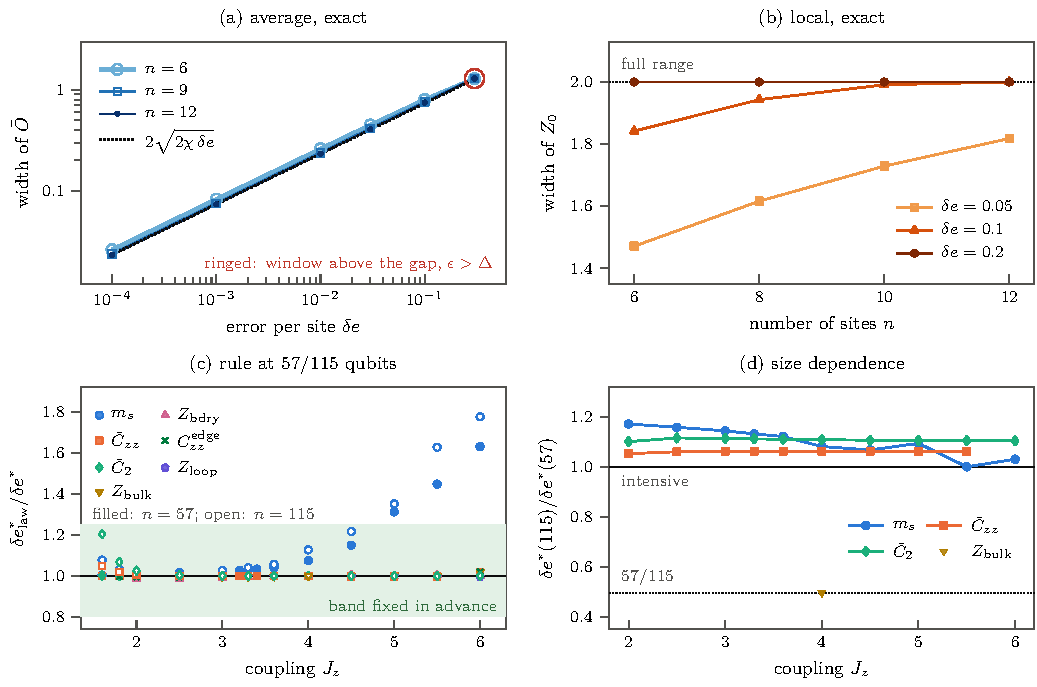
\includegraphics[width=\textwidth]{fig2_rule_pgf}%
\caption{\label{figS:rule}The rule, from exact checks to the dataset.
(a) Theorem~2 of the main text: exact two-sided width of the staggered magnetization of a comb ferrimagnet with an % (structural: theorem number)
extensively pinned sector, $n=6,9,12$ (exact diagonalization), against the error per site; dotted, the law % src: r3:t3_comb.txt (n = 6, 9, 12)
$2\sqrt{2\chi\de}$; ringed, windows above the gap. The width is intensive above the gap.
(b) Theorem~1: exact width of $Z_0$ in the periodic transverse-field Ising chain ($h=1.5$) at fixed error per % src: r3:t2_local.txt (h=1.5)
site, against $n$; the full range is $2$. % src: r3:t2_local.txt (w=2.000)
(c) The accuracy law at 57 and 115 qubits: ratio of the predicted to the computed $\des$ for the $116$ rows of the % src: def:phase3/full_runs/map/DECLARATION.md; figures/pgf_sm_method/export_check.txt (125 rows, 116 with law_ratio_out)
map with $\Jz\ge1.6$ for which it is stored (filled $n=57$, open $n=115$; no ratio is stored for eight local rows at
$n=57$, $\Jz\le2.0$, nor for $\Czz$ at $n=115$, $\Jz=6.0$); shaded, the band $[0.8,1.25]$ fixed in advance for the % src: def:phase3/full_runs/map/DECLARATION.md (C-D band; averaged labels, Jz >= 2.0)
averaged labels at $\Jz\ge2.0$. The outliers are $\ms$
at $\Jz\ge5$, where the ``$-$'' chain goes through the crossing to a reversed-domain state (an avoided crossing
at finite $n$).
(d) $\des(115)/\des(57)$: averages are intensive; the local $Z_{\rm bulk}$ follows $57/115$. % src: map:claims.C-E.rows (Z_bulk 0.4958)
Sources: Sec.~\ref{sm:checks} and the deposited map outputs.}
\end{figure}

\subsection{The certification map in detail}
\label{sm:moved_map}

\begin{table}[h]
\caption{\label{tabS:pubmap}Summary of the map on the public data (Sec.~\ref{sm:pubmap}; window of energy and mean % src: def:phase3/full_runs/real_data/DECLARATION.md
magnetization; $\tau=0.06|o_\GS|$). Columns 3--4: separation of two explicit states of the window, over $\tau$, at the % src: def:phase3/full_runs/real_data/DECLARATION.md (tau = 0.06 |O_GS|)
test coupling $\Jz=1.2$ and at $\Jz=1.6$, rounded down (not certified if $\ge1$). Column 5: lowest certified training
coupling; every training coupling above it is certified (in parentheses, with the certificates added after the
declaration; ``none'': no certificate was computed for the label). Column 6: certified training couplings out of $45$;
the counts are the same with the reference-free tolerance. Column 7: width of the exact interval over $\tau$ at
$\Jz=6.0$, rounded up. Column 8: factor by which the published energy error per site exceeds what a certificate
would need at the test couplings (smallest value over $\Jz=1.1$--$1.4$, rounded down). Generated from the stored
outputs of the map.}
\begin{ruledtabular}
\begin{tabular}{llcccccc}
Label & $n$ & sep.$/\tau$, $\Jz=1.2$ & sep.$/\tau$, $\Jz=1.6$ & certified from & certified/45 & $w/\tau$, $\Jz=6.0$ & accuracy needed \\
\hline
% generated by figures/sm_tables/make_rdmap.py from phase3/full_runs/real_data/out/map_rows.json, map_summary.json; phase3/full_runs/real_data/e1/map_e1/map_rows.json -- do not edit
$m_s$ & 57 & 16.01 & 7.39 & 3.5 & 26 & 0.218 & $>110$ \\
$\bar C_{zz}$ & 57 & 7.90 & 5.19 & 3.4 & 27 & 0.229 & $>57$ \\
$\bar C_{2}$ & 57 & 17.25 & 10.22 & none & 0 & -- & -- \\
$Z_{\rm bulk}$ & 57 & 42.40 & 24.50 & none & 0 & -- & -- \\
$Z_{\rm bdry}$ & 57 & 39.44 & 28.65 & none & 0 & -- & -- \\
$C_{zz}^{\rm edge}$ & 57 & 37.44 & 22.76 & none & 0 & -- & -- \\
$Z_{\rm loop}$ & 57 & 60.55 & 34.18 & none & 0 & -- & -- \\
\hline
$m_s$ & 115 & 12.31 & 6.71 & 4.0 (3.4) & 21 (27) & 0.145 & $>79$ \\
$\bar C_{zz}$ & 115 & 8.24 & 4.97 & 4.0 (3.6) & 21 (25) & 0.155 & $>49$ \\
$\bar C_{2}$ & 115 & 16.77 & 9.40 & none & 0 & -- & -- \\
$Z_{\rm bulk}$ & 115 & 13.42 & 6.29 & none & 0 & -- & -- \\
$Z_{\rm bdry}$ & 115 & 6.86 & 4.64 & none & 0 & -- & -- \\
$C_{zz}^{\rm edge}$ & 115 & 8.37 & 4.78 & none & 0 & -- & -- \\
$Z_{\rm loop}$ & 115 & 20.01 & 10.74 & none & 0 & -- & -- \\

\end{tabular}
\end{ruledtabular}
\end{table}

\begin{table}[h]
\caption{\label{tabS:map}Cross-check: summary of the figures-based map (Sec.~\ref{sm:figmap}; sector states, reading 1 % src: def:phase3/full_runs/map/DECLARATION.md
of the digitized energies; certified: window width $\le\tau=0.06|o_\GS|$, DMRG-referenced; not a property of the % src: def:phase3/full_runs/map/DECLARATION.md (tau = 0.06|O_GS|)
public labels). Columns 3--4: rigorous inner width at the lower window
over $\tau$ at the OOD point $\Jz=1.2$ (conditional on the assumed floor) and at $\Jz=1.6$ (not certified if $\ge1$). Column 5:
certification threshold $J^*$ at the central reading (with the $20\%$ margin in parentheses; ``none'': no threshold % src: derived: 0.8x / 1.2x windows = 20 % margin
within the training range). Column 6: certified training points out of $45$. Column 7: outer width over $\tau$ at the
digitized energy at the last computed point ($\Jz=6.0$; $^a$: $\Jz=4.0$). Column 8: range of $\des_{\rm law}/\des$
over the rows with $\Jz\ge2.0$. Generated from the deposited map outputs.}
\begin{ruledtabular}
\begin{tabular}{llcccccc}
Label & $n$ & $w/\tau$, $\Jz=1.2$ & $w/\tau$, $\Jz=1.6$ & $J^*$ (margin) & certified/45 & $w/\tau$, last & $\des_{\rm law}/\des$ \\
\hline
% generated by figures/make_table1.py from phase3/full_runs/map/laptop_analysis/summary_map.json
$m_s$ & 57 & 12.0 & 6.67 & 3.2 (3.4) & 29 & 0.21 & 1.01--1.63 \\
$\bar C_{zz}$ & 57 & 7.06 & 4.79 & 3.2 (3.4) & 29 & 0.23 & 1.00--1.02 \\
$\bar C_{2}$ & 57 & 15.6 & 9.43 & 4.0 (4.2) & 21 & 0.38 & 1.00--1.00 \\
$Z_{\rm bulk}$ & 57 & 36.4 & 22.5 & 6.0 (none) & 1 & 0.99 & 1.00--1.02 \\
$Z_{\rm bdry}$ & 57 & 35.8 & 24.9 & none (none) & 0 & 1.05 & 0.98--1.01 \\
$C_{zz}^{\rm edge}$ & 57 & 31.0 & 20.9 & 6.0 (none) & 1 & 0.99 & 1.00--1.02 \\
$Z_{\rm loop}$ & 57 & 56.2 & 32.4 & none (none) & 0 & 1.39 & 1.00--1.00 \\
\hline
$m_s$ & 115 & 10.6 & 6.28 & 3.1 (3.3) & 30 & 0.13 & 1.02--1.78 \\
$\bar C_{zz}$ & 115 & 6.84 & 4.79 & 3.1 (3.3) & 30 & 0.14 & 1.00--1.01 \\
$\bar C_{2}$ & 115 & 14.3 & 9.08 & 3.8 (3.9) & 23 & 0.24 & 1.00--1.03 \\
$Z_{\rm bulk}$ & 115 & -- & -- & -- & -- & 3.00$^{a}$ & 1.00--1.00 \\

\end{tabular}
\end{ruledtabular}
\end{table}

\emph{Two summaries.} Table~\ref{tabS:pubmap} summarizes the map on the public data and Table~\ref{tabS:map} the
figures-based map that it replaces as the basis of the paper. The rest of this subsection keeps the detail of the
figures-based map and of the thresholds of the model; each paragraph says which of the two it concerns.

\emph{Certified widths.} On the public data the exact intervals at $\Jz=6.0$ are $0.218$ and $0.229\,\tau$ wide % src: rdm:rows[n=57,Jz=6.0,label=m_s].exact.width_over_tau (0.21784); rdm:rows[n=57,Jz=6.0,label=Czz_bar].exact.width_over_tau (0.22822); derived: rounded up
($\ms$, $\Czz$; $n=57$) and $0.145$ and $0.155\,\tau$ ($n=115$). In the figures-based map the certified widths at % src: rdm:rows[n=115,Jz=6.0,label=m_s].exact.width_over_tau (0.14457); rdm:rows[n=115,Jz=6.0,label=Czz_bar].exact.width_over_tau (0.15457)
$\Jz=6.0$ were $0.21$--$0.23\,\tau$ ($n=57$) and $0.13$--$0.14\,\tau$ % src: map:row(57,6.0,m_s).at_dig.w_out/tau (0.211); map:row(57,6.0,Czz_bar) (0.225); map:row(115,6.0,m_s) (0.131); map:row(115,6.0,Czz_bar) (0.145)
($n=115$). With reading 1 every training point from $J^*$ up was certified there; reading 2 has no readable energy at
$\Jz=5.1$ ($n=57$) and therefore counts $28$ points, with the same $J^*$. % src: map:jstar.57_m_s_r2.n_certified_central (28); map:jstar.57_m_s_r2.J_star_central

\emph{Rigorous lower bounds.} The certified side need not rest on the reference ground energies. For every field
$\lambda$ and every sector state in the window, $\sigma\langle O\rangle\le[E-E_{\rm LB}(H-\sigma\lambda SO)]/(\lambda S)$
with $E_{\rm LB}$ any rigorous lower bound on a sector ground energy (Lemma~A). We obtain $E_{\rm LB}$ from a
local-consistency relaxation over clusters of five to nine sites, solved in dual form; its multipliers are rounded to % src: file:phase3/full_runs/rigor/RESULTS_v2.md
rationals and every cluster inequality is verified by exact integer elimination in a separate program
(Sec.~\ref{sm:rigor}). In the figures-based map what was then established is a chain of conditions: if (i) the dataset's states lie in the sector,
(ii) its energies are their Rayleigh quotients, and (iii) its energy lies below our certificate-side threshold
$E_{\rm up}$, then (iv) its label lies in an interval proved in exact arithmetic. Step (iii)
uses our DMRG ground energy and gap and the digitized energy ratio, and holds if each factor of the reading is within % src: file:phase3/full_runs/map/RESULTS.md; def:phase3/full_runs/map/DECLARATION.md
$\pm5\%$, the dataset's gap within $10\%$ of ours and its reference energy within $0.04\,r\Delta$ of ours; steps (i) % src: file:phase3/full_runs/map/RESULTS.md; def:phase3/full_runs/map/DECLARATION.md
and (ii) were assumptions. With the fields fixed in advance, the proved interval of step (iv) is at most $\tau$ wide for $13$ of the $14$ certified rows at % src: rig:verdicts.S1.n_certified (4); rig:verdicts.S2.n_certified (9); derived: 4 + 9 = 13 of 4 + 10 = 14
$n=57$ ($\ms$ and $\Czz$ at $\Jz=3.4$--$6.0$) and for all four rows tested at $n=115$ ($\Jz=4.0$ and $6.0$), at % src: rig:rows[n=57,Jz=3.4,label=Czz_bar].Jz; rig:rows[n=57,Jz=6.0,label=m_s].Jz; rig:verdicts.S3.n_certified (4); rig:rows[n=115,Jz=4.0,label=m_s].Jz; rig:rows[n=115,Jz=6.0,label=m_s].Jz
widths $0.004$--$0.10\,\tau$ above the referenced ones: $17$ of $18$ rows, with $\tau$ from DMRG ($16$ with the % src: derived: rig:rows[*].w_over_tau - map at_up w_out/tau over the 17 certified rows (0.0035-0.1004); derived: 4 + 9 + 4 = 17 of 18, and 16 of 18 with the reference-free tolerance (Table of Sec. S4)
reference-free tolerance). The exception is $\ms$ at $\Jz=3.4$, whose % src: rig:rows[n=57,Jz=3.4,label=m_s].Jz
referenced width is already $0.958\,\tau$ and whose rigorous width is $1.09\,\tau$. By the decision rule fixed in % src: map:row(57,3.4,m_s).at_up.w_out/tau (0.958); rig:rows[n=57,Jz=3.4,label=m_s].w_over_tau (1.0859)
advance, this one row rejects the block $\Jz=3.4$--$5.5$ at $n=57$, while the blocks $n=57$, $\Jz=4.0$ and $6.0$, and % src: rig:rows[n=57,Jz=3.4,label=m_s].Jz; rig:rows[n=57,Jz=5.5,label=m_s].Jz
$n=115$, $\Jz=4.0$ and $6.0$, are confirmed; the threshold with margin, $J^*=3.4$ at $n=57$, therefore rested on the
DMRG references. The ground energy at $\Jz=4.0$ is bracketed to $0.007\%$. Eight of the % src: rig1:H.0.levels.best.slack_rel_pct (0.0068); rig1:H.0.Jz
certificates were re-verified on a laptop with independent code (Sec.~\ref{sm:rigor}). These proofs hold at the
computed couplings; $J^*$, the counts of certified training points of that map, $\Ctwo$, the local rows and the other $n=115$
couplings remained referenced. On the public data the chain is shorter: (i) and (ii) are replaced by hypothesis H
and the published mean magnetization, (iii) by the published energy itself, and the interval of (iv) is proved for
every state with that energy and magnetization (Sec.~\ref{sm:public_exact}).

\emph{Local labels and the OOD point.} In the figures-based map, at the OOD point $\Jz=1.2$ the width of $\ms$ is $0.4617$ ($n=57$), % src: map:row(57,1.2,m_s).at_lo.w_in
conditional on the assumed floor. The bulk site and the edge correlation reach the line only at the last training point,
$\Jz=6.0$ ($0.99\,\tau$), and the loop stays at $1.39\,\tau$. At $n=115$, $\Jz=4.0$, the bulk site is $3.0\,\tau$ wide % src: map:row(57,6.0,Z_bulk).at_dig.w_out/tau (0.991); map:row(57,6.0,Czz_edge) (0.988); map:row(57,6.0,Z_loop) (1.388); map:row(115,4.0,Z_bulk).at_dig.w_out/tau (3.004)
($2.5\,\tau$ at $n=57$). On the public data, two explicit states with the published energy and mean magnetization % src: map:row(57,4.0,Z_bulk) (2.499)
have $\ms$ values $16.0\,\tau$ apart at $\Jz=1.2$, $n=57$, with no floor assumed (Table~\ref{tabS:pubmap}). % src: rdm:rows[n=57,Jz=1.2,label=m_s].explicit.width_over_tau (16.011)

\emph{The accuracy law at scale.} This paragraph concerns the model in the sector, with DMRG references. The accuracy law, with $\chi$ from the two smallest-field points of each chain,
predicts $\des$ to within a factor $0.997$--$1.22$ at all but six of the averaged rows with $\Jz\ge2.0$ % src: map:claims.C-D.range (0.9968); derived: recount of rows[*].de_star_law/de_star_out, max inside band 1.2162
[Fig.~\ref{figS:rule}(c)], the set fixed in advance; at smaller $\Jz$ the $115$-qubit outer bounds are too loose to
test the law or the ratio $\des(115)/\des(57)$. It fails at six rows, $\ms$ at $\Jz\ge5.0$, by factors up to $1.64$ ($n=57$) and $1.78$ % src: map:claims.C-D.outside (6 rows, 1.6301, 1.7752); derived: 1.6301 rounded up
($n=115$): there the ``$-$'' chain crosses to a reversed-domain state before the width reaches $\tau$, so the response
is not quadratic. The failure is in the over-confident direction, but the dataset's error lies at least $8.7$ times % src: map:row(57,5.0,m_s).f_out (8.784); derived: rounded down
below the computed $\des$ at those points with the digitized energies, and at least $8.8$ times with the public % src: rdm:rows[n=57,Jz=5.0,label=m_s].like.f_out (8.807)
ones, so no status changes. The law should be read as an upper estimate to be
confirmed by a chain where the order is strong; exact checks on bipartite trees, re-run with separate code, find the
same over-confidence, by factors of $1.8$--$4.1$, on the side opposing a pinned order (% src: file:phase3/full_runs/learning_ibm/crosschecks/thm_attack_output.txt (2.15766, 1.01041, 4.32830, 2.45903, 1.67264, 0.40529); derived: ratios 1.76-4.13
cross-check folder of the realistic learning test).

\emph{Agreement of the two bounds, and the size of the error.} For sector states, where both sides are computed they agree: at $n=57$
the inner and outer widths at the lower window differ by at most $1\%$ in every averaged row with $\Jz\ge1.6$ (for % src: file:phase3/full_runs/map/RESULTS.md (<= 1 %)
$\ms$ at $\Jz=1.6$: $0.3081$ against $0.3091$). The information limit is therefore computed, not only bounded. At % src: map:row(57,1.6,m_s).at_lo.w_in; map:row(57,1.6,m_s).at_lo.w_out (0.3091)
the certified points of the figures-based map the window is far below the in-sector gap: $\epsilon/\Delta_{\rm in}\le0.11$ at every certified % src: map:row(115,3.3,m_s).eps_over_gap_in (0.106)
row where the ratio is recorded (maximal at $n=115$, $\Jz=3.3$; at $n=57$ at most $0.041$, at $\Jz=3.6$, and $0.01$ % src: map:row(57,3.6,m_s).eps_over_gap_in (0.041); map:row(57,6.0,m_s).eps_over_gap_in (0.0097)
at $\Jz=6.0$; not recorded at $\Jz=3.4$). At the rows certified on the public data the published error is at most $0.043$ of that % src: map:row(57,6.0,m_s).Jz; map:row(57,3.4,m_s).Jz; map:row(115,4.0,m_s).eps_over_gap_in; derived: maximum 0.0427, at n = 115 and Jz = 4.0, of eps_pub times eps_over_gap_in over eps_dig, rounded up
gap where it is recorded ($0.066$ at $n=115$, $\Jz=3.6$, a row certified only with the added certificates). % src: map:row(115,3.6,m_s).eps_over_gap_in; derived: 0.0655 from eps_pub times eps_over_gap_in over eps_dig, rounded up
Every certified status lies in the range $\epsilon\le\bar\Delta_O/2$ of the two-sided bound of Ref.~\cite{manchanda2026}; % (formula)
what the uniform-in-$n$ statements add is the size dependence of the statuses. At $\Jz=1.6$ the digitized error is $0.58$ of % src: map:row(57,1.6,m_s).eps_over_gap_in (0.576)
the gap at $n=57$ and $1.22$ at $n=115$; the ``not certified'' statuses there follow from explicit witnesses. % src: map:row(115,1.6,m_s).eps_over_gap_in (1.216)

\emph{Simple witnesses and checks.} At $n=57$, $\Jz=1.6$, a matrix-product state of bond dimension $32$ already gives % src: def:phase3/full_runs/map/DECLARATION.md (chi in 16, 32, 64)
$97\%$ of the pure-state width: a generator of modest entanglement can land anywhere in these windows. The best single % src: map:minchi.57_1.6_m_s.chis.32.frac_of_full (0.968)
stored states there, without superposition, reach $0.3049$ of the hull width $0.3081$; the two pure states built as in % src: map:row(57,1.6,m_s).at_lo.w_pure (0.3049); map:row(57,1.6,m_s).at_lo.w_in (0.3081)
Lemma~B (the larger of bond dimension $320$) attain all of it (Sec.~\ref{sm:pure}). At $n=19$ the % src: file:phase3/full_runs/map/RESULTS.md (bond dimension 320)
outer widths agree with exact diagonalization to $0.43\%$; raising the bond dimension from $320$ to $480$ changes % src: file:phase3/full_runs/map/RESULTS.md (0.43 %)
$E_0$ by at most $3.5\times10^{-6}$; and our lowest gap to the $S^z=s-1$ sector matches the gap plotted in the % src: file:phase3/full_runs/map/RESULTS.md (3.5e-6)
dataset paper to within $0.81\%$ at every computed training coupling except $n=57$, $\Jz=1.6$, where the plotted marker % src: map:gates.G3_gap_record.rows (largest relative difference 0.00802 apart from n = 57, Jz = 1.6); derived: rounded up
is partly covered and our gap is $4.1\%$ and $5.1\%$ above the two readings (Sec.~\ref{sm:figmodel}). The authors' % src: map:gates.G3_gap_record.rows (0.0408 and 0.0509)
own DMRG, now public, agrees with our references to $1.9\times10^{-6}$ ($n=57$) and $3.01\times10^{-5}$ ($n=115$) in the % src: rdg:G4_57.max_abs_dE0 (1.872e-6); rdg:G4_115.max_abs_dE0 (3.010e-5)
ground energy and to $1.5\times10^{-4}\,\tau$ and $2.8\times10^{-4}\,\tau$ in the labels (Sec.~\ref{sm:public_checks}). % src: rdg:G4_57.max_abs_dO_over_tau (Z_bulk 1.457e-4); rdg:G4_115.max_abs_dO_over_tau (C2_bar 2.792e-4)

\subsection{The method class: mechanism, and estimates at the dataset's energy}

\begin{figure}[h]
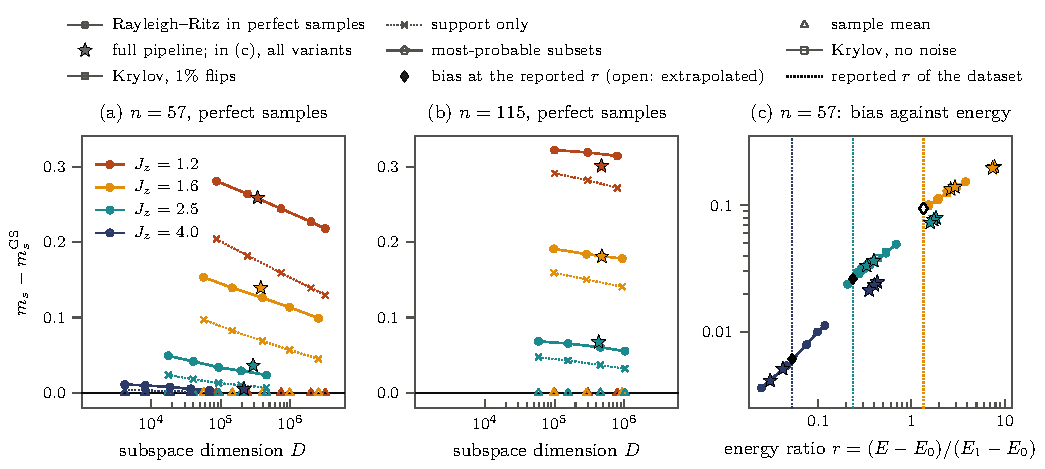
\includegraphics[width=\textwidth]{fig3_mechanism_pgf}%
\caption{\label{figS:mechanism}Origin of the bias in the emulated first stage of the method class. (a, b) Signed $\ms$ bias against subspace dimension for perfect samples of the
DMRG ground state: circles, Rayleigh--Ritz in the sampled configurations (what the method does); crosses, the ground
state projected on the same configurations (support only); triangles, the multiplicity-weighted sample mean (no
diagonalization); stars, the full emulated pipeline at the published budget. Colours: $\Jz$.
(c) $n=57$ at $\Jz=1.6$, $2.5$ and $4.0$ (no energy is reported at $\Jz=1.2$): the bias against the energy ratio
$r=(E-E_0)/(E_1-E_0)$ of the perfect samples (circles), the most-probable subsets (pentagons), the Krylov shot scans
without and with $1\%$ flips (open and filled squares) and every pipeline variant (stars); dotted lines, the dataset's % src: def:phase3/full_runs/method/DECLARATION.md (1 % floor)
reported $r$ (its Fig.~2, digitized); diamonds, the emulated bias read there (open where it is extrapolated beyond the % fig: Ref. [jaderberg2026] Fig. 2
sampled ratios), an estimate that assumes the dataset's pipeline follows the same bias--energy relation; the public
labels now test that assumption (Sec.~\ref{sm:publiccurve}: its ratios stay inside the declared band at $n=57$ and it overstates the bias at $n=115$, so its declared test fails).
Sources: deposited method outputs.}
\end{figure}

\emph{Mechanism.} Replacing the Krylov sampler by perfect samples of the DMRG ground state, cut to the same subspace
dimension, reproduces the bias: $+0.258$ against $+0.259$ at $n=57$, $\Jz=1.2$ (ratio $0.997$; $1.05$ at $n=115$) % src: meth:decisions.D2_n57.dm_s_gs_at_D (0.2578); meth:decisions.D2_n57.dm_s_primary (0.2586); meth:decisions.D2_n57.M; meth:decisions.D2_n115.M
[Fig.~\ref{figS:mechanism}(a,b)]. The samples themselves are unbiased: the multiplicity-weighted mean of the same
perfect samples reproduces the reference $\ms$ to $6\times10^{-4}$ in every case. The bias arises in two steps of the % src: file:phase3/full_runs/method/RESULTS.md (6e-4)
diagonalization: keeping only the sampled support already over-orders ($+0.175$ of the $+0.258$), because the % src: file:phase3/full_runs/method/RESULTS.md (+0.175)
missing weight sits on configurations with more defects, and Rayleigh--Ritz adds the rest by moving weight back
toward well-connected, N\'eel-like configurations. Device-like noise adds $+0.02$ to $+0.07$ and the random-flip % src: file:phase3/full_runs/method/RESULTS.md (+0.02 to +0.07)
recovery changes the bias by at most $0.005$: neither creates it. The most-probable subsets fall on the same curve as % src: file:phase3/full_runs/method/RESULTS.md (-0.000 to -0.005)
the samples, so the best subspace of a given size has the same bias. At $n=115$, $\Jz=1.2$, $8\times10^5$ sampled % src: file:phase3/full_runs/method/RESULTS.md (8x10^5)
configurations capture $0.2\%$ of the ground-state weight and the bias stays at $+0.314$: what controls it is the % src: file:phase3/full_runs/method/laptop_post/results_tables.md (W 0.0020, +0.314)
captured weight, which collapses with $n$ near the isotropic point. Perfect samples and most-probable subsets are
the diagnostics with which Ref.~\cite{gaberle2026} found, up to $20$ qubits, that configuration counts grow exponentially with size; % (structural: sizes in the cited work)
here they fix the sign of the label error. A miniature exact calculation with separate code on a $12$-site comb reproduces % src: file:paper/data/crosschecks/check4_output.txt (n=12; frac>0 1.00)
the sign in every repetition (Sec.~\ref{sm:checks}).

\emph{Estimates at the dataset's energy (conditional).} Assuming---untested---that the dataset's full pipeline
follows the bias--energy relation of all emulated families [Fig.~\ref{figS:mechanism}(c)], the bias could be read at
the energy the dataset reports. At $n=57$ this reading over-predicts the dataset paper's published unsigned % (sizes)
$\langle Z_i\rangle$ errors by about a fifth to a third (Table~\ref{tab:meth_at_energy}), so it is an upper estimate; at $\Jz=1.6$, $2.5$ and $4.0$ it gives % (couplings)
$+0.094$, $+0.026$ and $+0.006$. Assuming in addition the sign of the emulation, a second estimate multiplies the % src: meth:bias_at_ibm_energy.57_1.6.dm_s (0.0942); meth:bias_at_ibm_energy.57_2.5.dm_s (0.0262); meth:bias_at_ibm_energy.57_4.0.dm_s
dataset paper's unsigned $\langle Z_i\rangle$ error (its Supp.\ Fig.~11) by the slope of the emulated states:
$+0.080$, $+0.020$ and $+0.005$ at the same couplings, and $+0.159$ and $+0.146$ at $\Jz=1.2$ ($n=57$, $115$). Both % src: meth:dZ_matched.57_1.6.dm_s (0.0797); meth:dZ_matched.57_2.5.dm_s (0.0200); meth:dZ_matched.57_4.0.dm_s; meth:dZ_matched.57_1.2.dm_s (0.1589); meth:dZ_matched.115_1.2.dm_s (0.1460)
are conditional estimates for the method class at the dataset's published quality, made before the labels were known
to be public; neither is a measurement of the dataset's labels. The measurement is in Sec.~\ref{sm:publictests}, and
Sec.~\ref{sm:emu} sets it next to these estimates ($+0.077$, $+0.022$ and $+0.006$ at $\Jz=1.6$, $2.5$ and $4.0$ for % src: rdp:sizes.57.P5.rows[Jz=1.6].Delta (0.0771); rdp:sizes.57.P5.rows[Jz=2.5].Delta (0.0221); rdp:sizes.57.P5.rows[Jz=4.0].Delta (0.0063)
$n=57$; $+0.157$ and $+0.144$ at $\Jz=1.2$ for $n=57$ and $115$). % src: rdp:sizes.57.P5.rows[Jz=1.2].Delta (0.1574); rdp:sizes.115.P5.rows[Jz=1.2].Delta (0.1441)
Under these assumptions they would place the method at $45$--$76\%$ of the maximal excess of order % src: file:phase3/full_runs/method/RESULTS.md (45-76 %)
that the energy permits ($66$--$96\%$ for the emulated states at their own energies). Where the map certifies, the % src: file:phase3/full_runs/method/RESULTS.md (66-96 %)
emulated bias is below $\tau/2$ at every computed point, even at the emulation's own (higher) energies. The reading of
the colour scale of the dataset paper's Fig.~4 is described, with its limits, in Sec.~\ref{sm:emu}.

\subsection{Learning on the benchmark: the per-label shifted labels in full}

These numbers are per label: each label is taken from its own extremal window state, so the bond set is not a
dataset that one state could produce (Sec.~\ref{sm:proofs}, Corollary~2, scope). With labels shifted inside the same % (structural: theorem/corollary numbers)
windows the standard intervals still cover about $0.90$ of their own labels, but only $0.72$ (M1) and $0.63$ (M2) of % src: lm1:coverage.advL5.SC.nn.covO_id (0.904); lm1:coverage.advL5.SC.avg.covT_id (0.718); lm2:coverage.advL5.SC.avg.covT_id (0.634)
the true averages and $0.82$ and $0.60$ of the true single bonds, for the declared shift toward less order; toward % src: lm1:coverage.advL5.SC.nn.covT_id (0.821); lm2:coverage.advL5.SC.nn.covT_id (0.599)
more order, $0.55$--$0.79$. The better learner is the more exposed: the same shift is a larger fraction of its % src: lm2:coverage.advM5.SC.nn.covT_id (0.5517); lm1:coverage.advM5.SC.nn.covT_id (0.785)
narrower intervals. Normalized conformal scores and ensembles do no better (Sec.~\ref{sm:learn}). With realistic labels
the energy-calibrated intervals are $1.60$ (averages) and $1.30$ (single bonds) times wider than the standard intervals for % src: lver:D5.avg.value (1.598); lver:D5.nn.value (1.302)
M1, and $1.15$--$2.0$ times over both learners and both $\de$; with shifted labels, up to $2.5$ times toward less % src: file:phase3/full_runs/learning/RESULTS.md (1.15-2.0; up to 2.5×)
order and $4.1$ toward more order (diagonal pairs, M2). % src: derived: lm2 coverage.advM5 CSC.diag.wid_id / SC.diag.wid_id = 0.4237/0.1040 = 4.07 (Table S19)

\emph{The band rule.} Statement (a) of Proposition~2 yields a rule without a free threshold: answer where % (structural: proposition number)
$W(x)\le\tau$. With M1 it answers $99.8\%$ of the queries on averages and none on single bonds, and every answer lay % src: lver:D6.a_avg (0.9983); lver:D6.a_nn (0.0)
within $\tau$ of the prediction of the same learner trained on exact labels, also out of distribution. It does not
bound the learner's own error: with realistic labels $3\%$ of its answers on averages miss the truth by more than % src: file:phase3/full_runs/learning/RESULTS.md (3 % of its answers)
$\tau/2$. With M2 it answers only $14$--$16\%$ of the averages, because M2 amplifies label errors through a large % src: file:phase3/full_runs/learning/RESULTS.md (14-16 %)
$\|a(x)\|_1$. At $\de=10^{-3}$ rule (c) with the band-based energy-calibrated intervals (CB of Sec.~\ref{sm:learn}, which decides per input) answers about half of the average queries, with at most % src: file:phase3/full_runs/learning/RESULTS.md (5e-3; 1e-3)
$0.9\%$ missing; under the shift of the input distribution $1.7\%$ of its answers miss at $\de=5\times10^{-3}$, % src: lm2:abstention.advL1|avg|id|0.08.rule.CB_mid.exceed_given_answer (0.0089); lm1:abstention.gen5|avg|ood|0.08.rule.CB_mid.exceed_given_answer (0.0168); file:phase3/full_runs/learning/RESULTS.md (5e-3)
$23\%$ at $10^{-3}$ (M1). A rule calibrated on generated labels controls the error against them, not against the % src: lm1:abstention.gen1|avg|ood|0.08.rule.CB_mid.exceed_given_answer (0.2277); file:phase3/full_runs/learning/RESULTS.md (5e-3; 1e-3)
truth: with shifted labels $12\%$ of its answers miss the truth by more than $\tau/2$, while it misses its own labels % src: lver:D7.e_NC (0.1219)
in $4\%$ of them. Ranking queries by the energy-interval width orders them no better than ranking by the conformal width % src: file:phase3/full_runs/learning/RESULTS.md (own-label exceedance 0.038)
or the ensemble spread: the risk--coverage curves agree within $1$--$5\%$. % src: file:phase3/full_runs/learning/RESULTS.md (1-5 %)

\section{Exploratory bias analysis}
\label{sec:biaslaw}

This section supports Sec.~V of the main text. The analysis was made after the data were in hand and has no prior
declaration. Code and outputs: \texttt{phase3/full\_runs/bias\_law/}. The tests of the same curve that were declared
afterwards are in Sec.~\ref{sec:declared} (new emulated labels) and Sec.~\ref{sm:publictests} (the public labels).

\emph{Identity.} Let $P$ project on a fixed configuration set $S$, $E_S(h)$ be the lowest eigenvalue of $P(H+hO)P$ with
a nondegenerate eigenvector at $h=0$, $E_0(h)$ the lowest eigenvalue of $H+hO$ in the sector, with the same assumption,
and $\delta(h)=E_S(h)-E_0(h)$. By the variational principle $\delta(h)\ge0$. The Hellmann--Feynman theorem gives
$E_S'(0)=\langle O\rangle_S$ and $E_0'(0)=\langle O\rangle_\GS$, so $\langle O\rangle_S-\langle O\rangle_\GS=\delta'(0)$.
Inside $S$ the same theorem applied to a coupling $\Jz$ gives $\partial_{\Jz}E_S=\langle\partial_{\Jz}H\rangle_S$ when
$S$ is held fixed, which suggests why the slope of a family of subspace energies reproduces the biased label.
For a label diagonal in the configuration basis and a small weight outside $S$, both the bias and the energy error
are of second order in the coupling to the complement, so the bias is linear in the energy error~\cite{white2007}.
In density-matrix renormalization and selected configuration interaction, observables are often extrapolated against
a truncation or energy error at one size~\cite{white2007,stoudenmire2012,damour2023}.
That is the limit of small error, and it is not the regime of most of our data: the local log-log slope of the $n=19$
curves is $0.74$--$0.90$ at $\de=10^{-4}$--$10^{-3}$ and $0.34$--$0.68$ at $10^{-2}$--$10^{-1}$ (couplings with at % src: file:paper/reviews/R10_2026-11-12/scratch/phys-declared-stats/extras_bias2_out.txt (0.748, 0.897; 0.348, 0.670); derived: ranges rounded outward, with the fit windows 1e-4, 1e-3, 1e-2, 1e-1 as in bias_law.py
least three curve points in the window and $\Jz\le5$; the analysis script fits three couplings and stores $0.85$ and % src: file:paper/reviews/R10_2026-11-12/scratch/phys-declared-stats/extras_bias2_out.txt (J=5.0); blw:nulls.log_slope.2.5_low (0.853)
$0.90$ for the lower window, $0.39$ to $0.56$ for the upper one), and at $\Jz=1.2$ perfect samples cut to % src: blw:nulls.log_slope.4.0_low (0.897); blw:nulls.log_slope.2.5_high (0.390); blw:nulls.log_slope.4.0_high (0.561)
$7.3\times10^5$ ($n=57$) and $8.0\times10^5$ ($n=115$) configurations capture $0.33$ and $0.002$ of the ground-state % src: file:phase3/full_runs/method/RESULTS.md (733 k, W 0.33; 799 k, W 0.0020); derived: 733 k and 799 k written as 7.3e5 and 8.0e5
weight (cf.\ Ref.~\cite{bonilla2026spectral}). We have no derivation of the transfer across sizes.

\emph{Curves.} At $n=19$ the exact ground state in the sector (dimension $75\,582$) is cut to its most probable % src: file:phase3/full_runs/bias_law/code/bias_law.py (n = 19); derived: C(19,8) = 75582; rdp:independent_recomputation.n19_from_scratch_vs_stored.dim (75582)
configurations at $26$ truncation levels per coupling and $H$ is diagonalized in each set; at a label's energy the % src: rdp:independent_recomputation.n19_from_scratch_vs_stored.levels (26); derived: 26 entries per curve in inputs/n19_curves.json
bias is read by interpolation in $\sqrt{\de}$. Curves from stored states use a least-squares cubic in $\sqrt{\de}$
without constant term (all families) or interpolation through the origin and four variants (main-text Fig.~4(b)). % (structural: figure number)

\emph{Spread around the curve.} The curve at $n=19$ is on a heavy-hex patch of distance $3$; the emulated states are % src: file:phase3/full_runs/method/code/graphs/hh_d3.json (3)
on patches of distance $5$ and $7$ and the device labels on distance $5$ only. At the four couplings of main-text % src: def:phase3/full_runs/map/DECLARATION.md (distance 5, 7)
Fig.~4(a), $\Jz=1.2$, $1.6$, $2.5$ and $4.0$, the ratio of the bias to the curve over the $127$ stored emulated % src: file:phase3/full_runs/real_data/checks/r11/fp_bias_curve_recompute_out.txt (127 states)
states is $0.876$--$1.244$; over all stored couplings ($195$ states) it is $0.873$--$1.413$. Nine states lie outside % src: blw:nulls.ratio_to_curve_min (0.8761); blw:nulls.ratio_to_curve_max (1.2432); file:phase3/full_runs/real_data/checks/r11/fp_bias_curve_recompute_out.txt (195 states, ratio min 0.8735, max 1.4122); derived: ranges rounded outward
the range of the four couplings: two at $n=115$, $\Jz=1.3$ and $1.4$, and seven variants with device-like noise at % src: file:phase3/full_runs/real_data/checks/r11/fp_bias_curve_recompute_out.txt (states outside the range of the four couplings: 9 of 195 (2 below, 7 above); n=115 J=1.4, n=115 J=1.3)
$\Jz=5.0$ and $6.0$, whose bias is at most $0.3\,\tau$. For the primary labels alone, at all $25$ coupling--size % src: file:phase3/full_runs/real_data/checks/r11/fp_bias_curve_recompute_out.txt (couplings [5.0, 6.0]; greatest raw bias among them raw=0.293 tau); derived: 0.293 rounded up to 0.3; derived: 14 + 11 = 25 pairs (blw:n19_curve.57.raw.n, blw:n19_curve.115.raw.n)
pairs, the ratio is $0.882$--$1.235$, and for our six device readings $0.912$--$1.172$. Every one of the $195$ % src: file:phase3/full_runs/real_data/checks/r11/fp_bias_curve_recompute_out.txt (primary-label ratio over all 25 coupling-size pairs (14 + 11): 0.8829-1.2347; 0.9127 .. 1.1712; 195 states); derived: ranges rounded outward
states and of the six device readings lies between the ground state and the N\'eel state, in bias and in energy.

\emph{Labels of the primary states.} Table~\ref{tab:bias_rows} lists, for $\ms$, the miss of the label as generated, of
the truth at $n=19$ used as the answer, and of the label corrected with the curve from the truncated exact ground state % src: file:phase3/full_runs/bias_law/code/bias_law.py (n = 19)
at $n=19$. The corrected miss is at most $0.18\,\tau$ at $n=57$ and $0.98\,\tau$ at $n=115$. At $n=115$ the % src: blw:n19_curve.57.corrected.max (0.1737); blw:n19_curve.115.corrected.max (0.9707); derived: maxima rounded up to 0.18 and 0.98
correction with the $n=57$ curve misses by $0.09\,\tau$ on average (at most $0.31\,\tau$); the % src: blw:classical_tie_115.corr57.mean (0.090); blw:classical_tie_115.corr57.max (0.302); derived: 0.302 rounded up to 0.31
classical two-point extrapolations from $n=19$ and $57$ miss by $0.10$, $0.04$ and $0.01\,\tau$ for $a+b/n$, $a+b\,N_e/n$ % src: blw:nulls.a_b_over_n.mean (0.102); blw:nulls.a_b_edges_over_n.mean (0.037); blw:nulls.a_b_over_sqrt_n.mean (0.014)
and $a+b/\sqrt n$, the last being the form expected for an open two-dimensional patch. The correction does not
simply return the truth of the calibration size, which misses by $0.26\,\tau$ (at most $0.66\,\tau$). The % src: blw:nulls.truth57_alone.mean (0.259); blw:nulls.truth57_alone.max (0.652); derived: 0.652 rounded up to 0.66
parameter-free chord of the main text misses by $0.37$, $0.11$ and $0.12\,\tau$ at $n=57$, at % src: blw:nulls.chord_57.mean (0.367); blw:nulls.chord_115.mean (0.105); blw:nulls.chord_device.mean (0.124)
$n=115$ and on the device (at most $1.4$, $0.28$ and $0.31\,\tau$). % src: blw:nulls.chord_57.max (1.386); blw:nulls.chord_115.max (0.2718); blw:nulls.chord_device.max (0.3033); derived: maxima rounded up, 0.2718 to 0.28 and 0.3033 to 0.31
\def\SMcap{Exploratory correction of $\ms$ with the curve from exact $n=19$: miss in units of $\tau$, primary emulated labels.}\def\SMlab{tab:bias_rows}
% generated by figures/make_sm_bias_law.py from phase3/full_runs/bias_law/out/results.json -- do not edit

{\footnotesize\setlength{\tabcolsep}{5pt}\renewcommand{\arraystretch}{1.2}
\begin{longtable}{llcccc}
\caption{\SMcap}\label{\SMlab}\\
\toprule
\rule[-3pt]{0pt}{11.5pt} $n$ & $J_z$ & $\delta e$ & as generated & truth at $n=19$ & corrected \\
\midrule
\rule[-3pt]{0pt}{11.5pt} 57 & 1.1 & 0.04954 & 8.42 & 1.47 & 0.11 \\
\rule[-3pt]{0pt}{11.5pt} 57 & 1.2 & 0.04328 & 6.73 & 1.34 & 0.17 \\
\rule[-3pt]{0pt}{11.5pt} 57 & 1.3 & 0.03792 & 5.44 & 1.19 & 0.17 \\
\rule[-3pt]{0pt}{11.5pt} 57 & 1.4 & 0.03281 & 4.43 & 1.05 & 0.16 \\
\rule[-3pt]{0pt}{11.5pt} 57 & 1.6 & 0.02476 & 3.01 & 0.81 & 0.11 \\
\rule[-3pt]{0pt}{11.5pt} 57 & 1.8 & 0.01880 & 2.10 & 0.63 & 0.06 \\
\rule[-3pt]{0pt}{11.5pt} 57 & 2.0 & 0.01451 & 1.51 & 0.49 & 0.02 \\
\rule[-3pt]{0pt}{11.5pt} 57 & 2.2 & 0.01120 & 1.10 & 0.39 & 0.00 \\
\rule[-3pt]{0pt}{11.5pt} 57 & 2.5 & 0.00733 & 0.68 & 0.29 & 0.02 \\
\rule[-3pt]{0pt}{11.5pt} 57 & 3.0 & 0.00379 & 0.32 & 0.19 & 0.01 \\
\rule[-3pt]{0pt}{11.5pt} 57 & 3.5 & 0.00220 & 0.16 & 0.13 & 0.01 \\
\rule[-3pt]{0pt}{11.5pt} 57 & 4.0 & 0.00137 & 0.09 & 0.10 & 0.00 \\
\rule[-3pt]{0pt}{11.5pt} 57 & 5.0 & 0.00075 & 0.04 & 0.06 & 0.00 \\
\rule[-3pt]{0pt}{11.5pt} 57 & 6.0 & 0.00051 & 0.02 & 0.04 & 0.00 \\
\midrule
\rule[-3pt]{0pt}{11.5pt} 115 & 1.1 & 0.08694 & 9.23 & 2.07 & 0.97 \\
\rule[-3pt]{0pt}{11.5pt} 115 & 1.2 & 0.07865 & 7.57 & 1.85 & 0.91 \\
\rule[-3pt]{0pt}{11.5pt} 115 & 1.3 & 0.07124 & 6.29 & 1.63 & 0.83 \\
\rule[-3pt]{0pt}{11.5pt} 115 & 1.4 & 0.06461 & 5.29 & 1.43 & 0.70 \\
\rule[-3pt]{0pt}{11.5pt} 115 & 1.6 & 0.05321 & 3.84 & 1.10 & 0.48 \\
\rule[-3pt]{0pt}{11.5pt} 115 & 2.0 & 0.03690 & 2.22 & 0.67 & 0.21 \\
\rule[-3pt]{0pt}{11.5pt} 115 & 2.5 & 0.02392 & 1.24 & 0.41 & 0.07 \\
\rule[-3pt]{0pt}{11.5pt} 115 & 3.0 & 0.01589 & 0.75 & 0.27 & 0.02 \\
\rule[-3pt]{0pt}{11.5pt} 115 & 4.0 & 0.00741 & 0.30 & 0.14 & 0.00 \\
\rule[-3pt]{0pt}{11.5pt} 115 & 5.0 & 0.00371 & 0.14 & 0.09 & 0.01 \\
\rule[-3pt]{0pt}{11.5pt} 115 & 6.0 & 0.00197 & 0.07 & 0.06 & 0.01 \\
\bottomrule
\end{longtable}}


\emph{Device labels and further states.} For our device labels (three couplings, each read with and without
recovery) the $n=19$ curve lowers the mean miss from $4.3$ to $0.34\,\tau$; the greatest, $0.78\,\tau$, is at % src: blw:device.raw.mean (4.27); blw:device.n19.mean (0.338); blw:device.n19.max (0.7709); derived: 0.7709 rounded up to 0.78
$\Jz=1.2$, against $0.26$ and $0.06\,\tau$ at $1.6$ and $4.0$ (with recovery). A curve built from the emulated % src: file:phase3/full_runs/real_data/checks/r11/fp_bias_curve_recompute_out.txt (corrected [0.771, 0.253, 0.056]); derived: 0.253 rounded up to 0.26
states at $n=57$ brings the device labels to $0.07\,\tau$ (at most $0.16\,\tau$) and the $52$ stored states of % src: blw:device.emu57.mean (0.065); blw:device.emu57.max (0.159); blw:families_57_to_115.raw.n (52)
$7$ families at $n=115$, at $\Jz=1.2$, $1.6$ and $2.5$, from $4.3$ to $0.18\,\tau$ (at most $0.44\,\tau$). The label % src: blw:families_57_to_115.n_families (7); blw:families_57_to_115.raw.mean (4.28); blw:families_57_to_115.corrected.mean (0.176); blw:families_57_to_115.corrected.max (0.4363); derived: 0.4363 rounded up to 0.44
of the declared device job at $\Jz=6.0$, obtained after this analysis, lies $8\%$ above the $n=19$ curve (a miss of % src: file:paper/reviews/R10_2026-11-12/scratch/phys-declared-stats/extras_bias_out.txt (ratio 1.079); derived: 1.079 is 8 per cent above one
$0.007\,\tau$ after the correction against $0.095\,\tau$ before); it is one point at strong order, where the bias is % src: file:paper/reviews/R10_2026-11-12/scratch/phys-declared-stats/extras_bias_out.txt (corrected miss 0.007 tau; raw miss 0.095 tau)
small.

\emph{A model trained on corrected labels.} The cubic model of main-text Sec.~VI, trained on the labels corrected
with the $n=19$ curve, misses the test couplings by $0.3$--$1.2\,\tau$ at $n=57$ and $0.8$--$2.0\,\tau$ at $n=115$, % src: blw:learner.57.corrected.min (0.291); blw:learner.57.corrected.max (1.175); blw:learner.115.corrected.min (0.799); blw:learner.115.corrected.max (1.995)
against $4.5$--$8.8\,\tau$ and $5.3$--$8.9\,\tau$ with the labels as generated, at most $0.2\,\tau$ with exact % src: blw:learner.57.raw.min (4.46); blw:learner.57.raw.max (8.78); blw:learner.115.raw.min (5.25); blw:learner.115.raw.max (8.91); blw:learner.57.exact.max (0.200)
labels, and $1.05$--$1.47\,\tau$ and $1.43$--$2.07\,\tau$ for quoting the truth at $n=19$. % src: blw:nulls.small_truth_test_57_min (1.05); blw:nulls.small_truth_test_57_max (1.47); blw:nulls.small_truth_test_115_min (1.43); blw:nulls.small_truth_test_115_max (2.07)

\emph{What is generic, and what the reading needs.} Near the isotropic point the labels are far along the path from
the ground state to the N\'eel state: at $n=115$ and $\Jz\le1.6$ the bias reaches $84$--$90\%$ of its ceiling % src: file:phase3/full_runs/bias_law/code/bias_law.py (J <= 1.6); blw:nulls.ceiling_pct_min (84.0); blw:nulls.ceiling_pct_max (90.2)
$1-m_s^{\rm GS}$. The reading needs $\de$, hence $E_0$, at the target size. At $n=115$ an estimate of $E_0$ linear in
the numbers of sites and edges gives the same mean miss ($0.39\,\tau$), but that fit uses DMRG at $n=57$; at $n=57$, % src: blw:no_reference_115.mean (0.389)
scaling $E_0$ from $n=19$ alone per bond or per site gives $0.48$ or $1.04\,\tau$, no better than quoting the truth % src: blw:nulls.e0_57_per_bond.mean (0.48); blw:nulls.e0_57_per_site.mean (1.04)
at $n=19$ ($0.59\,\tau$). % src: blw:n19_curve.57.small_truth.mean (0.585)

\emph{Internal checks.} A biased family looks consistent, even though its configuration set changes with $\Jz$: at
$\Jz\le2.5$ (a range chosen in the analysis script, after the data, where the label error is large) the slope of the % src: file:phase3/full_runs/bias_law/code/bias_law.py (J <= 2.5)
emulated energy curve misses the reference $\Czz$ by $0.95$--$1.05$ times the error of the label itself ($n=57$); % src: blw:internal_checks.57.slope_error_over_label_error_min (0.953); blw:internal_checks.57.slope_error_over_label_error_max (1.053)
over all couplings the same ratio is $0.17$--$2.42$. Using every sample as a variational state at every other % src: file:paper/reviews/R10_2026-11-12/scratch/phys-declared-stats/extras_bias2_out.txt (5.0: 0.174, 6.0: 2.415); derived: range rounded outward
coupling exposes less than $1\%$ of the energy error. Checks of this kind did not reveal the bias here. % src: blw:internal_checks.57.hull_fraction_max (0.0061); derived: 0.0061 < 1 %

\emph{An earlier comparison with published errors, now superseded.} Before the labels were known to be public we
compared the curve with the unsigned errors that the dataset paper reports: at the dataset's digitized energies, a
cubic fitted to the unsigned site error of the $n=57$ emulated states predicted errors $18$--$52\%$ above the % src: blw:published.over_min (18.4); blw:published.over_max (51.5)
published ones at the five points where both numbers existed ($18$, $39$ and $29\%$ at $\Jz=1.6$, $2.5$ and $4.0$ % src: blw:published.rows (five rows; 18.39, 39.37, 29.49)
for $n=57$). The public labels allow the comparison at every coupling, with the sign, and it replaces this one: at
the couplings that decide the declared test their bias is $0.80$--$1.05$ of the $n=19$ curve at $n=57$ and % src: rdp:sizes.57.P5.all.ratio_range_deciding (0.8029, 1.0455)
$0.60$--$0.82$ at $n=115$ (Sec.~\ref{sm:publiccurve}). % src: rdp:sizes.115.P5.all.ratio_range_deciding (0.6087, 0.8122); derived: range rounded outward

\emph{Other models.} Table~\ref{tab:bias_other} applies the same truncation to square-lattice XXZ, frustrated
$J_1$--$J_2$ Heisenberg and random Heisenberg models on $3\times4$, $4\times4$ and $4\times5$ open lattices, comparing % src: file:phase3/full_runs/bias_law/code/generality.py (sizes (3, 4), (4, 4), (4, 5))
curves at equal energy error per site. The error falls by factors of $2.6$ to more than $20$, but the corrected value % src: blw:other_models.raw_over_corrected_min (2.60); derived: the stored maximum 42.0 = 0.42/0.01 is a ratio of two-decimal values, at least 0.415/0.015 = 27.7, so "more than 20" is safe
beats the truth of the small system in all $8$ combinations at strong order and in $1$ of $14$ near the isotropic % src: blw:other_models.wins_strong (8); blw:other_models.n_strong (8); blw:other_models.wins_hard (1); blw:other_models.n_hard (14)
point or with frustration or disorder; the combinations are of coupling, label and calibration size, not independent
trials. These are small systems and one truncation family, so the table shows where the
transfer breaks, not its size at large $n$.
\def\SMcap{Transfer of the bias curve to $n=20$ at equal energy error per site: mean miss in units of $\tau$. Last column: the truth of the calibration size used as the answer.}\def\SMlab{tab:bias_other} % src: file:phase3/full_runs/bias_law/inputs/generality.txt (20)
% generated by figures/make_sm_bias_law.py from phase3/full_runs/bias_law/out/results.json -- do not edit

{\footnotesize\setlength{\tabcolsep}{5pt}\renewcommand{\arraystretch}{1.2}
\begin{longtable}{lcccc}
\caption{\SMcap}\label{\SMlab}\\
\toprule
\rule[-3pt]{0pt}{11.5pt} model and label & size & as generated & corrected & small-system truth \\
\midrule
\rule[-3pt]{0pt}{11.5pt} square XXZ $J_z=1.2$ $\bar C_{zz}$ & 12 & 6.54 & 1.08 & 0.28 \\
\rule[-3pt]{0pt}{11.5pt} square XXZ $J_z=1.2$ $\bar C_{zz}$ & 16 & 5.87 & 0.35 & 0.25 \\
\rule[-3pt]{0pt}{11.5pt} square XXZ $J_z=1.2$ $m_s^2$ & 12 & 13.62 & 3.60 & 1.18 \\
\rule[-3pt]{0pt}{11.5pt} square XXZ $J_z=1.2$ $m_s^2$ & 16 & 12.76 & 1.22 & 0.09 \\
\rule[-3pt]{0pt}{11.5pt} square XXZ $J_z=2.0$ $\bar C_{zz}$ & 12 & 1.09 & 0.23 & 0.63 \\
\rule[-3pt]{0pt}{11.5pt} square XXZ $J_z=2.0$ $\bar C_{zz}$ & 16 & 1.09 & 0.09 & 0.22 \\
\rule[-3pt]{0pt}{11.5pt} square XXZ $J_z=2.0$ $m_s^2$ & 12 & 1.50 & 0.24 & 0.75 \\
\rule[-3pt]{0pt}{11.5pt} square XXZ $J_z=2.0$ $m_s^2$ & 16 & 1.64 & 0.12 & 0.28 \\
\rule[-3pt]{0pt}{11.5pt} square XXZ $J_z=4.0$ $\bar C_{zz}$ & 12 & 0.34 & 0.04 & 0.07 \\
\rule[-3pt]{0pt}{11.5pt} square XXZ $J_z=4.0$ $\bar C_{zz}$ & 16 & 0.37 & 0.01 & 0.02 \\
\rule[-3pt]{0pt}{11.5pt} square XXZ $J_z=4.0$ $m_s^2$ & 12 & 0.42 & 0.03 & 0.06 \\
\rule[-3pt]{0pt}{11.5pt} square XXZ $J_z=4.0$ $m_s^2$ & 16 & 0.42 & 0.01 & 0.02 \\
\rule[-3pt]{0pt}{11.5pt} frustrated $J_1$--$J_2$ Heisenberg $J_2=0.3$ $\bar C_{zz}$ & 12 & 9.88 & 2.09 & 0.82 \\
\rule[-3pt]{0pt}{11.5pt} frustrated $J_1$--$J_2$ Heisenberg $J_2=0.3$ $\bar C_{zz}$ & 16 & 8.79 & 0.81 & 0.33 \\
\rule[-3pt]{0pt}{11.5pt} frustrated $J_1$--$J_2$ Heisenberg $J_2=0.5$ $\bar C_{zz}$ & 12 & 8.30 & 2.18 & 0.92 \\
\rule[-3pt]{0pt}{11.5pt} frustrated $J_1$--$J_2$ Heisenberg $J_2=0.5$ $\bar C_{zz}$ & 16 & 9.64 & 0.70 & 0.39 \\
\rule[-3pt]{0pt}{11.5pt} random Heisenberg (Huang-type) seed 1 $\bar C_{zz}$ & 12 & 9.32 & 3.58 & 1.56 \\
\rule[-3pt]{0pt}{11.5pt} random Heisenberg (Huang-type) seed 1 $\bar C_{zz}$ & 16 & 9.32 & 0.65 & 1.06 \\
\rule[-3pt]{0pt}{11.5pt} random Heisenberg (Huang-type) seed 2 $\bar C_{zz}$ & 12 & 8.98 & 1.63 & 0.14 \\
\rule[-3pt]{0pt}{11.5pt} random Heisenberg (Huang-type) seed 2 $\bar C_{zz}$ & 16 & 8.98 & 0.72 & 0.63 \\
\rule[-3pt]{0pt}{11.5pt} random Heisenberg (Huang-type) seed 3 $\bar C_{zz}$ & 12 & 9.69 & 2.14 & 0.98 \\
\rule[-3pt]{0pt}{11.5pt} random Heisenberg (Huang-type) seed 3 $\bar C_{zz}$ & 16 & 10.17 & 3.50 & 0.33 \\
\bottomrule
\end{longtable}}


\emph{Instance-specific labels.} Random Heisenberg couplings, per-bond labels at $n=20$, four targets, calibration on % src: file:phase3/full_runs/bias_law/code/instance_test.py (4 targets; 8 instances)
eight other $4\times4$ instances (twenty rows). Mean miss: $10.41\,\tau$ for the labels as generated, $3.17\,\tau$ % src: blw:instance_test.raw (10.41); blw:instance_test.corrected (3.17)
corrected by a linear map at matched energy error, $2.55\,\tau$ for a ridge model on local couplings with no quantum % src: blw:instance_test.classical (2.55)
data, and $1.66\,\tau$ for the corrected labels combined with the local couplings. The corrected labels alone beat the % src: blw:instance_test.both (1.66)
classical model in $6$ of the $20$ rows, and combined with the local couplings in $20$ of $20$; the classical model is % src: blw:instance_test.corrected_beats_classical (6); blw:instance_test.rows (20); blw:instance_test.both_beats_classical (20)
weak, and the labels are truncations of the target's exact ground state. The sample is small; Sec.~\ref{sec:declared}
tests the question under declared rules, against much stronger classical estimates.

\section{Declared tests}
\label{sec:declared}

This section supports Sec.~V of the main text. The rules were written down, and their SHA-256 checksum computed on our own machine, minutes before the virtual % src: derived: SHA-256 is a name, 256
machine started; the device test's protocol was completed in two addenda checksummed later, each before any processor
use; no third-party registry was used. Declaration, code, outputs and dated deviations: \texttt{phase3/full\_runs/final\_tests/}. All $128$ % src: file:phase3/full_runs/final_tests/RESULTS.md (128)
computing tasks finished; the declared device job ran later than declared (see Deviations below). Statements concern the emulated method class and our own device data. The tests of
the same kind on the public labels, declared later and after an initial look at those data, are in
Sec.~\ref{sm:publictests}; there the curve fails its second condition at $n=115$.

\emph{Test of the curve at new couplings.} The test is out of sample, at couplings where neither labels nor predictors
existed; it is blind in that sense only. Table~\ref{tab:ft_a} gives the seven primary labels. The rule, written with
the exploratory values in hand ($0.06$ and $0.39\,\tau$; ratios $0.88$--$1.24$), asked for a mean miss of at % src: blw:n19_curve.57.corrected.mean (0.062); blw:n19_curve.115.corrected.mean (0.385); file:phase3/full_runs/real_data/checks/r11/fp_bias_curve_recompute_out.txt (primary-label ratio over all 25 coupling-size pairs (14 + 11): 0.8829-1.2347); derived: rounded outward, 0.8829 to 0.88 and 1.2347 to 1.24
most $0.2\,\tau$ at $n=57$ and $0.6\,\tau$ at $n=115$, and for all seven ratios of the bias to the curve to lie in % src: fta:rule.limit57 (0.2); fta:rule.limit115 (0.6)
$[0.75,1.3]$; comparisons with the chord and the classical forms were stated separately. The means are $0.06$ and % src: def:phase3/full_runs/final_tests/DECLARATION.md (0.75, 1.3); fta:rule.mean57 (0.0619)
$0.34\,\tau$, the greatest single misses $0.14$ and $0.59\,\tau$ (both at $\Jz=1.5$), and the ratios % src: fta:rule.mean115 (0.3398); fta:summary.57.miss_curve19.max (0.1322); fta:summary.115.miss_curve19.max (0.5840); derived: maxima rounded up, 0.1322 to 0.14 and 0.5840 to 0.59
$0.88$--$1.06$. The curve beats the chord at $n=57$ in the mean ($0.06$ against $0.23\,\tau$), % src: fta:rule.mean57 (0.0619); fta:rule.ratio_min (0.8849); fta:rule.ratio_max (1.0568); fta:versus.57.miss_chord (0.2342)
though at $\Jz=2.8$ the chord is slightly better, and it loses at $n=115$ ($0.34$ against $0.11\,\tau$), where the ratio % src: file:phase3/full_runs/final_tests/RESULTS.md (2.8); fta:versus.115.miss_chord (0.1054)
stays below one at all three couplings, the deficit of Sec.~\ref{sec:biaslaw}. At $n=115$ the curve from the emulated
states at $n=57$ misses by $0.06\,\tau$, the truth at $n=57$ by $0.24\,\tau$, and the three classical forms by $0.08$, % src: fta:versus.115.miss_curve57 (0.0562); fta:summary.115.truth57.mean (0.236); fta:versus.115.miss_a_b_over_n (0.0824)
$0.02$ and $0.01\,\tau$. Labels and predictors at these couplings did not exist before the test. DMRG references at % src: fta:versus.115.miss_a_b_edges_over_n (0.0189); fta:versus.115.miss_a_b_over_sqrt_n (0.0110)
$n=57$, $\Jz=2.8$ and $3.2$ did exist; they were recomputed, not read. Time steps at $\Jz=1.7$, $2.8$, $3.2$ are % src: file:phase3/full_runs/final_tests/RESULTS.md (2.8, 3.2, 1.7)
interpolated, and the emulation at $n=115$ is the one that misses its declared energy condition (Sec.~\ref{sm:emu}). At $n=57$ the classical forms do not
apply, and the only comparator besides the chord is the truth at $n=19$, which the curve beats ($0.06$ against $0.51\,\tau$). % src: fta:summary.57.miss_curve19.mean (0.0619); fta:summary.57.small_truth.mean (0.505)
The test had limited power: the seven couplings lie between those of the exploration, and linear interpolation of the
exploratory misses gives $0.06$ and $0.35\,\tau$, within $0.007$ and $0.02\,\tau$ of the outcome at every point, % src: ftp:interp_mean.57 (0.0635); ftp:interp_mean.115 (0.3511); ftp:interp_maxdiff.57 (0.0063); ftp:interp_maxdiff.115 (0.0193); derived: 0.0063 rounded up to 0.007
and the seven ratios lie within $0.0031$ ($n=57$) and $0.0011$ ($n=115$) of the interpolated exploratory ratios, % src: file:phase3/full_runs/real_data/checks/r11/fp_bias_curve_recompute_out.txt (interpolated ratio ... max |difference| 0.0031; max |difference| 0.0011)
against a declared band about a hundred times wider. The residual of the curve is not noise: it is negative near the
isotropic point and positive at strong order, so a mean over couplings understates the miss where it matters.
\def\SMcap{Test of the bias curve at new couplings (emulated labels): miss of $m_s$ in units of $\tau$, primary label at each point. Ratio: bias over curve.}\def\SMlab{tab:ft_a}
% generated by figures/make_sm_final_tests.py from phase3/full_runs/final_tests/analysis/ -- do not edit

{\footnotesize\setlength{\tabcolsep}{3pt}\renewcommand{\arraystretch}{1.2}
\begin{longtable}{llcccccccc}
\caption{\SMcap}\label{\SMlab}\\
\toprule
\rule[-3pt]{0pt}{11.5pt} $n$ & $J_z$ & $\delta e$ & as generated & curve & ratio & chord & truth at $n=19$ & $a+b/n$ & $a+b/\sqrt n$ \\
\midrule
\rule[-3pt]{0pt}{11.5pt} 57 & 1.5 & 0.02859 & 3.64 & 0.13 & 0.965 & 0.54 & 0.92 & -- & -- \\
\rule[-3pt]{0pt}{11.5pt} 57 & 1.7 & 0.02145 & 2.50 & 0.085 & 0.967 & 0.35 & 0.71 & -- & -- \\
\rule[-3pt]{0pt}{11.5pt} 57 & 2.8 & 0.00493 & 0.43 & 0.017 & 1.041 & 0.013 & 0.22 & -- & -- \\
\rule[-3pt]{0pt}{11.5pt} 57 & 3.2 & 0.00305 & 0.24 & 0.013 & 1.057 & 0.037 & 0.16 & -- & -- \\
\rule[-3pt]{0pt}{11.5pt} 115 & 1.5 & 0.05865 & 4.49 & 0.58 & 0.885 & 0.13 & 1.25 & 0.12 & 0.016 \\
\rule[-3pt]{0pt}{11.5pt} 115 & 1.7 & 0.04844 & 3.32 & 0.40 & 0.893 & 0.13 & 0.97 & 0.091 & 0.015 \\
\rule[-3pt]{0pt}{11.5pt} 115 & 2.8 & 0.01867 & 0.91 & 0.039 & 0.959 & 0.054 & 0.31 & 0.035 & 0.001 \\
\bottomrule
\end{longtable}}


\emph{Do labels add information?} Heavy-hex lattice at $n=57$, bonds scaled by factors uniform in $[0.5,1.5]$, six test % src: def:phase3/full_runs/final_tests/DECLARATION.md (0.5, 1.5)
instances at each of $\Jz=1.6$ and $2.5$, with $57$ site and $64$ bond labels per instance and DMRG truth at bond dimension % src: def:phase3/full_runs/final_tests/DECLARATION.md (1.6, 2.5, 64)
$320$. The labels come from the same first stage as in the main text, with $1\%$ flips and recovery. Every learned model % src: def:phase3/full_runs/final_tests/DECLARATION.md (320); def:phase3/full_runs/final_tests/DECLARATION.md (1 %)
was trained on $600$ disordered $n=19$ instances per coupling, with no $n=57$ truth. The quantum estimates regress the % src: def:phase3/full_runs/final_tests/DECLARATION.md (600)
difference between truth and label on the local couplings, the label, the energy error and its square root, and the
products of the label with these two; the
primary family of training states is the truncated exact ground state, the secondary one the same first stage at $n=19$.
The classical estimates are a regression on the local couplings trained on the truth at $n=19$, the exact ground state
of a cluster of $13$ or $19$ sites around each label, with an open boundary or with cut bonds replaced by a mean field % src: def:phase3/full_runs/final_tests/DECLARATION.md (13)
(two self-consistent passes), and a stack of the $13$-site clusters and the local couplings. The best classical estimate % src: def:phase3/full_runs/final_tests/DECLARATION.md (13)
is the one with the smallest mean miss on the test instances, an oracle choice that favours the classical side. The rule
required a miss at least $25\%$ below it and a win in at least five of six instances, at both couplings. DMRG on the % src: def:phase3/full_runs/final_tests/DECLARATION.md (0.25); derived: 0.25 = 25 %
target was reported but kept out of the decisive set, since at some bond dimension it must equal the truth.

Table~\ref{tab:ft_b} gives the outcome. The primary quantum estimate loses in $12$ of $12$ instances (Table~\ref{tab:ft_b_inst}), % src: derived: 6 + 6 = 12 instances
with a change of $-806\%$ (bootstrap over instances, $95\%$ range $-874$ to $-719\%$) and $-2006\%$ ($-2103$ to % src: ftb:Jz.1.6.q_top.improvement (-8.0595); ftb:Jz.1.6.q_top.boot_low (-8.7348); ftb:Jz.1.6.q_top.boot_high (-7.1983); ftb:Jz.2.5.q_top.improvement (-20.0565); ftb:Jz.2.5.q_top.boot_low (-21.0269); derived: 95 % range of the bootstrap, rounded outward (-719.83 to -719)
$-1932\%$). No secondary line changes this: the estimates without a target-size reference and the secondary family also % src: ftb:Jz.2.5.q_top.boot_high (-19.3217)
win in no instance. The correction is still real: it lowers the miss $4.5$ and $4.2$ times against the label as generated. % src: derived: 3.303 / 0.742 = 4.5; derived: 0.867 / 0.2073 = 4.2
The $19$-site cluster with a mean-field boundary is $9$ and $21$ times closer to the truth than the primary estimate % src: ftp:ratio_to_best_1.6.q_top (9.06); ftp:ratio_to_best_2.5.q_top (21.06)
($7.0$--$10.1$ and $19.6$--$23.3$ times in the single instances) and $5$ and $20$ times closer than the secondary one % src: file:paper/reviews/R10_2026-11-12/scratch/phys-declared-stats/recompute_table2_out.txt (min 7.09 max 10.08; min 19.65 max 23.29); derived: ranges rounded outward; ftp:ratio_to_best_1.6.q_kry (5.29); ftp:ratio_to_best_2.5.q_kry (19.90)
($4.6$--$6.8$ and $18.9$--$22.4$). Ranges of the mean miss over the six instances, at $\Jz=1.6$ and $2.5$: label % src: file:paper/reviews/R10_2026-11-12/scratch/phys-declared-stats/recompute_table2_out.txt (min 4.61 max 6.80; min 18.90 max 22.39); derived: ranges rounded outward
$3.0$--$3.6$ and $0.81$--$0.89$; primary estimate $0.61$--$0.92$ and $0.18$--$0.24$; secondary $0.39$--$0.50$ and % src: file:paper/reviews/R10_2026-11-12/scratch/phys-declared-stats/stats_gain_out.txt (3.02, 3.53; 0.819, 0.887; 0.613, 0.914; 0.184, 0.238; 0.393, 0.496); derived: ranges rounded outward
$0.18$--$0.23$; regression $0.85$--$1.00$ and $0.21$--$0.26$; open $19$-site cluster $0.80$--$1.06$ and % src: file:paper/reviews/R10_2026-11-12/scratch/phys-declared-stats/stats_gain_out.txt (0.182, 0.224; 0.858, 1; 0.217, 0.26; 0.806, 1.06); derived: ranges rounded outward
$0.13$--$0.19$; embedded $13$-site cluster $0.13$--$0.21$ and $0.024$--$0.028$; embedded $19$-site cluster % src: file:paper/reviews/R10_2026-11-12/scratch/phys-declared-stats/stats_gain_out.txt (0.131, 0.183; 0.134, 0.2; 0.0241, 0.0273); derived: ranges rounded outward
$0.065$--$0.095$ and $0.008$--$0.012$; DMRG at bond dimension $32$, $0.039$--$0.071$ and $0.003$--$0.007$. DMRG at % src: file:paper/reviews/R10_2026-11-12/scratch/phys-declared-stats/stats_gain_out.txt (0.0658, 0.0946; 0.00813, 0.0116; 0.0397, 0.0701; 0.00308, 0.00619); def:phase3/full_runs/final_tests/DECLARATION.md (32); derived: ranges rounded outward
that bond dimension is closer to the truth than the embedded $19$-site cluster in all $12$ instances. % src: file:paper/reviews/R10_2026-11-12/scratch/phys-declared-stats/recompute_table2_out.txt (dmrg32 better in 6/6 instances, at both couplings); fts:test_b_instances_total (12)
Here a cluster with a mean-field boundary is already close to exact, while with an open boundary it is not. The
locality of gapped ground states~\cite{deroeck2015,trivedi2022,teufel2026,osborne2007} would explain the outcome,
although, under a standard complexity assumption, a gap alone does not make ground-state properties efficiently
computable without data~\cite{huang2022}, and we did not measure the gap or the correlation length of these
instances. Against the regression on the same local couplings, a comparison added after the outcome was known
and not part of the declared rule, the labels help in the mean: the primary estimate lowers the
miss by $19\%$ and $14\%$, the secondary by $53\%$ and $19\%$. % src: ftp:gain_over_reg_1.6.q_top (19.4); ftp:gain_over_reg_2.5.q_top (13.8); ftp:gain_over_reg_1.6.q_kry (53.0); ftp:gain_over_reg_2.5.q_kry (18.54); derived: 18.54 rounded to 19
Per instance the primary estimate is better than the regression in $4$ of $6$ instances at $\Jz=1.6$ (changes of % src: file:paper/reviews/R10_2026-11-12/scratch/phys-declared-stats/stats_gain_out.txt (better in 4/6)
$-37$ to $+6\%$) and in $6$ of $6$ at $2.5$; at $1.6$ the gain is in the site labels ($0.94$ against $1.32$, in % src: file:paper/reviews/R10_2026-11-12/scratch/phys-declared-stats/stats_gain_out.txt (per-instance [-27.9, -19.2, 2.9, 5.1, -36.0, -36.3]; better in 6/6; sites only: means 0.943 vs 1.321); derived: range rounded outward, -36.3 to -37 and 5.1 to 6
$6$ of $6$ instances) and the bond labels are unchanged ($0.563$ against $0.564$, better in $3$ of $6$). The % src: file:paper/reviews/R10_2026-11-12/scratch/phys-declared-stats/stats_gain_out.txt (bonds only: means 0.563 vs 0.564, better in 3/6)
secondary estimate is better than the regression in $6$ of $6$ instances at both couplings. All eight quantum-side % src: file:paper/reviews/R10_2026-11-12/scratch/phys-declared-stats/stats_gain_out.txt (q_kry vs reg: better in 6/6)
fits selected the greatest length of the declared grid; in a re-fit made during review at $\Jz=1.6$ (those at $2.5$ % src: file:phase3/full_runs/real_data/checks/r11/fp_counts_out.txt (fits that selected the greatest length of the declared grid {2, 4, 8}: 8 of 8)
did not finish), five other random-feature seeds change the mean miss of the primary estimate to $0.72$--$0.74$ from % src: file:paper/reviews/R10_2026-11-12/scratch/phys-declared-stats/summarize_refits_out.txt (five other seeds 0.7236-0.7361); derived: range rounded outward
$0.74$, and lengths beyond the grid with the penalty chosen on the test instances, which favours the quantum side, % src: ftb:Jz.1.6.mean.q_top (0.742)
lower it by $9\%$, against the factor of $9$ that separates it from the cluster. % src: file:paper/reviews/R10_2026-11-12/scratch/phys-declared-stats/summarize_refits_out.txt (oracle beyond the grid 0.6749 (-9.0 %)); ftp:ratio_to_best_1.6.q_top (9.06)
Not tested: a model that combines the label with embedded clusters, device labels, couplings closer to the isotropic point, other
disorder, and any regime that DMRG cannot reach. The generated labels have an energy error per site of $0.026$--$0.029$ % src: fts:label_de_1.6.min (0.0263); fts:label_de_1.6.max (0.0289)
and $0.0085$--$0.0094$, $2.4$--$2.6$ and $2.0$--$2.1$ times the dataset's digitized error on the uniform model at the % src: fts:label_de_2.5.min (0.00853); fts:label_de_2.5.max (0.00935); fts:label_de_1.6.ratio_min (2.40); fts:label_de_1.6.ratio_max (2.64); fts:label_de_2.5.ratio_min (1.95); fts:label_de_2.5.ratio_max (2.14)
same couplings. Recorded single-core times per instance: $181$--$228$\,s for all cluster estimates together, % src: fts:seconds_per_instance.clusters (181.4, 227.9)
$50$--$63$\,s and $61$--$77$\,s for DMRG on the target at bond dimension $32$ and $64$, and $771$--$1050$\,s for the % src: fts:seconds_per_instance.dmrg32 (49.97, 63.39); fts:seconds_per_instance.dmrg64 (60.52, 77.42); def:phase3/full_runs/final_tests/DECLARATION.md (32, 64); fts:seconds_per_instance.emulation (771.0, 1050.1)
classical emulation of the generator; the training of the learned models is not included.
\def\SMcap{Mean miss on disordered lattices at $n=57$ over six instances and $121$ labels, in units of $6\%$ of the mean absolute label of each type.}\def\SMlab{tab:ft_b} % src: def:phase3/full_runs/final_tests/DECLARATION.md (121); derived: 0.06 = 6 %
% generated by figures/make_sm_final_tests.py from phase3/full_runs/final_tests/analysis/ -- do not edit

{\footnotesize\setlength{\tabcolsep}{5pt}\renewcommand{\arraystretch}{1.2}
\begin{longtable}{llcc}
\caption{\SMcap}\label{\SMlab}\\
\toprule
\rule[-3pt]{0pt}{11.5pt} estimate & uses & $J_z=1.6$ & $J_z=2.5$ \\
\midrule
\rule[-3pt]{0pt}{11.5pt} label as generated & quantum & 3.30 & 0.87 \\
\rule[-3pt]{0pt}{11.5pt} label with correction (primary) & quantum & 0.74 & 0.21 \\
\rule[-3pt]{0pt}{11.5pt} same, ground energy without target-size reference & quantum & 0.77 & 0.21 \\
\rule[-3pt]{0pt}{11.5pt} correction trained on the first stage at $n=19$ & quantum & 0.43 & 0.20 \\
\rule[-3pt]{0pt}{11.5pt} same, without reference & quantum & 0.42 & 0.18 \\
\rule[-3pt]{0pt}{11.5pt} regression on local couplings & classical & 0.92 & 0.24 \\
\rule[-3pt]{0pt}{11.5pt} open cluster, 13 sites & classical & 2.20 & 0.71 \\
\rule[-3pt]{0pt}{11.5pt} open cluster, 19 sites & classical & 0.92 & 0.16 \\
\rule[-3pt]{0pt}{11.5pt} stack on 13-site clusters & classical & 0.24 & 0.030 \\
\rule[-3pt]{0pt}{11.5pt} embedded cluster, 13 sites & classical & 0.16 & 0.025 \\
\rule[-3pt]{0pt}{11.5pt} embedded cluster, 19 sites (best classical) & classical & 0.082 & 0.010 \\
\midrule
\rule[-3pt]{0pt}{11.5pt} DMRG on the target, bond dimension 32 & outside the rule & 0.0507 & 0.00431 \\
\rule[-3pt]{0pt}{11.5pt} DMRG on the target, bond dimension 64 & outside the rule & 0.0040 & 0.00015 \\
\bottomrule
\end{longtable}}

\def\SMcap{Miss per test instance on disordered lattices, same units as Table~\ref{tab:ft_b}.}\def\SMlab{tab:ft_b_inst}
% generated by figures/make_sm_final_tests.py from phase3/full_runs/final_tests/analysis/ -- do not edit

{\footnotesize\setlength{\tabcolsep}{5pt}\renewcommand{\arraystretch}{1.2}
\begin{longtable}{ccccc}
\caption{\SMcap}\label{\SMlab}\\
\toprule
\rule[-3pt]{0pt}{11.5pt} instance & \multicolumn{2}{c}{$J_z=1.6$} & \multicolumn{2}{c}{$J_z=2.5$} \\
\rule[-3pt]{0pt}{11.5pt}  & best classical & label with correction & best classical & label with correction \\
\midrule
\rule[-3pt]{0pt}{11.5pt} 0 & 0.066 & 0.663 & 0.008 & 0.189 \\
\rule[-3pt]{0pt}{11.5pt} 1 & 0.085 & 0.743 & 0.012 & 0.238 \\
\rule[-3pt]{0pt}{11.5pt} 2 & 0.093 & 0.882 & 0.009 & 0.184 \\
\rule[-3pt]{0pt}{11.5pt} 3 & 0.095 & 0.914 & 0.010 & 0.218 \\
\rule[-3pt]{0pt}{11.5pt} 4 & 0.086 & 0.613 & 0.010 & 0.204 \\
\rule[-3pt]{0pt}{11.5pt} 5 & 0.066 & 0.637 & 0.010 & 0.210 \\
\bottomrule
\end{longtable}}


\emph{Device labels with proved intervals.} The stored configurations of the device job at $\Jz=4.0$ were rebuilt: same
subspace, of dimension $218\,647$, every configuration in the sector, and the Rayleigh quotient of the rounded vector % src: ftc:C1.rec.D (218647); derived: 218 647 = D
computed in rational arithmetic, which agrees with the stored float to $5\times10^{-14}$. With the stored certificates % src: ftc:C1.check_E_vs_stored (4.26e-14); derived: 4.26e-14 rounded up to 5e-14
this gives the two-sided intervals of Table~\ref{tab:ft_c}, with no DMRG value and no digitized figure. The same was
done for the declared job at $\Jz=6.0$ (with recovery: dimension $364\,045$, every configuration in the sector, rational and float % src: file:phase3/full_runs/final_tests/RESULTS.md (6.0); ft3:C3.rec.D (364045)
energies within $10^{-13}$), with the $18$ certificates at that coupling, $12$ stored and $6$ new. Here $\tau$ is $6\%$ % src: derived: |E_float - E_exact| = 8.5e-14 J (out_c3b_20261110T164846Z/out/c/rq_C_J6.0_rec.json) <= 1e-13; def:phase3/full_runs/final_tests/ADDENDUM_C3b.md (18; 12 stored + 6 new); derived: 0.06 = 6 %
of the lower end of $|O|$. The intervals contain the labels; all are wider than $\tau$ except those at $\Jz=6.0$. At % src: file:phase3/full_runs/final_tests/RESULTS.md (6.0); ft3:C3.rec.m_s.below_tau (true); ft3:C3.rec.Czz_bar.below_tau (true)
$\Jz=4.0$ the certificates were reused, not re-verified, and that interval had been evaluated once by hand before the % src: file:phase3/full_runs/qpu/RESULTS.md (4.0)
declaration, which says so. Each interval is a statement about the stored classical vector and holds whatever the
device measured; the bit-order checks support that its configurations come from the declared circuits. The stored
record holds the exact rational energy and a checksum of the rounded integer vector, not the vector. In a rebuild
made during review with the declared code, the subspaces of the four cases (both jobs, with recovery and with
post-selection) were reproduced exactly, the rounded vector was not reproduced bit for bit, and the exact energies of
the rebuilt vectors differ from the stored ones by less than $10^{-25}$, with intervals equal to the twelve digits % src: file:phase3/full_runs/real_data/checks/r11/fp_device_rebuild_out.txt (greatest |exact E rebuilt minus stored| over the four cases: 2.3e-26 (below 1e-25: True)); derived: 2.3e-26 < 1e-25
compared. The integer vectors are to be deposited with an integer-only checking script.
\needspace{160pt}% (layout) keep Table S32 (eight rows) on one page (2026-11-10: its last row had fallen alone onto the next page)
\def\SMcap{Device labels at $J_z=4.0$ and $6.0$ with intervals proved in exact arithmetic.}\def\SMlab{tab:ft_c} % src: file:phase3/full_runs/qpu/RESULTS.md (4.0); file:phase3/full_runs/final_tests/RESULTS.md (6.0)
% generated by figures/make_sm_final_tests.py from phase3/full_runs/final_tests/analysis/ -- do not edit

{\footnotesize\setlength{\tabcolsep}{5pt}\renewcommand{\arraystretch}{1.2}
\begin{longtable}{lcccc}
\caption{\SMcap}\label{\SMlab}\\
\toprule
\rule[-3pt]{0pt}{11.5pt} state & label & proved interval & width & width$/\tau$ \\
\midrule
\rule[-3pt]{0pt}{11.5pt} device, $J_z=4.0$, with recovery, $m_s$ & $0.98249$ & $[0.86843,\,0.99692]$ & 0.1285 & 2.47 \\
\rule[-3pt]{0pt}{11.5pt} device, $J_z=4.0$, with recovery, $\bar C_{zz}$ & $-0.98011$ & $[-0.99508,\,-0.88794]$ & 0.1071 & 2.01 \\
\rule[-3pt]{0pt}{11.5pt} device, $J_z=4.0$, postselected, $m_s$ & $0.98314$ & $[0.86391,\,0.99837]$ & 0.1345 & 2.59 \\
\rule[-3pt]{0pt}{11.5pt} device, $J_z=4.0$, postselected, $\bar C_{zz}$ & $-0.98084$ & $[-0.99659,\,-0.88492]$ & 0.1117 & 2.10 \\
\rule[-3pt]{0pt}{11.5pt} device, $J_z=6.0$, with recovery, $m_s$ & $0.98697$ & $[0.96325,\,0.99211]$ & 0.0288 & 0.50 \\
\rule[-3pt]{0pt}{11.5pt} device, $J_z=6.0$, with recovery, $\bar C_{zz}$ & $-0.98529$ & $[-0.99283,\,-0.96012]$ & 0.0327 & 0.57 \\
\rule[-3pt]{0pt}{11.5pt} device, $J_z=6.0$, postselected, $m_s$ & $0.98753$ & $[0.96156,\,0.99260]$ & 0.0310 & 0.54 \\
\rule[-3pt]{0pt}{11.5pt} device, $J_z=6.0$, postselected, $\bar C_{zz}$ & $-0.98590$ & $[-0.99305,\,-0.95824]$ & 0.0348 & 0.61 \\
\bottomrule
\end{longtable}}


\emph{The declared device run.} At $\Jz=6.0$ a simulation calibrated on the device job gave a mean energy error of $0.29$, % src: ftc:C2.gate.eps_sim (0.2892); file:phase3/full_runs/final_tests/RESULTS.md (6.0)
below the declared limit of $0.48$, which is $0.8$ of the threshold for an interval below $\tau$. The same simulation at % src: ftc:C2.gate.limit (0.4782); def:phase3/full_runs/final_tests/ADDENDUM_C3.md (0.8)
$\Jz=4.0$ reproduced the device error within $1.2\%$ ($0.835$, the mean of three seeds that give $0.81$--$0.86$, % src: derived: 1 - 0.9887 = 1.1 %, 0.835 / 0.8256 = 1.2 %; ftc:C2.validation_eps_J4.sim (0.8350); file:paper/reviews/R10_2026-11-12/scratch/phys-declared-stats/recompute_c3_out.txt (0.8141, 0.851); derived: range rounded outward
against $0.826$). On the day of the other tests the run % src: ftc:C2.validation_eps_J4.device (0.8256)
was not submitted. This was a deviation from the declared procedure, whose backend rule selected the device below and
required the run: the device used before had pairs with a reported error of one and offered no layout, and the only
device with a layout scored $1.25$ expected two-qubit errors per step against $0.79$. Scaling every error by that ratio, % src: file:phase3/full_runs/final_tests/RESULTS.md (1.252); file:phase3/full_runs/final_tests/RESULTS.md (0.790)
an exploratory check not in the declaration and a crude estimate of a device we have no data from, gives $1.22$ % src: ftx:noise_scan_eps.1.5852.mean (1.2237)
(three seeds, $1.0$--$1.4$). Two % src: ftx:noise_scan_eps.1.5852 (seeds 1.013, 1.288, 1.371)
days later the device used before offered a layout again, at $0.85$ errors per step, and we reversed the decision. A % src: derived: 0.8493 (def ADDENDUM_C3b.md, score at preparation) rounded to 0.85
second addendum, checksummed before the job was prepared, kept the declared protocol, decision rule and analysis and
added only conditions able to stop the run: that device alone, with no fall-back, and a score of at most $0.95$, about % src: def:phase3/full_runs/final_tests/ADDENDUM_C3b.md (0.95)
the score up to which the scan stays below the limit. The job was submitted on 2026-11-08 with $179$\,s of free % src: def:phase3/full_runs/final_tests/ADDENDUM_C3b.md (179); file:phase3/full_runs/final_tests/jobs/C_20261108/submit.json (2026-11-08)
processor time left and a cap of $150$\,s. It ran on 2026-11-10 and used $119$\,s; both bit-order checks passed % src: file:phase3/full_runs/final_tests/jobs/C_20261108/submit.json (150); file:phase3/full_runs/final_tests/RESULTS.md (2026-11-10; 119.0 s)
(smallest site agreement $0.9536$). Its exact Rayleigh quotient was computed on the same virtual machine as the other % src: file:phase3/full_runs/final_tests/RESULTS.md (0.9536)
tests, with the declared code and versions, and its interval, in exact rational arithmetic, on a laptop from the
fetched outputs, as the declaration allows; the noiseless control does not depend on the device and was not rerun. The label $\ms=0.98697$ lies in the proved interval $[0.96325,0.99211]$, $0.50\,\tau$ % src: ft3:C3.rec.m_s_label (0.986971); ft3:C3.rec.m_s.lo (0.963251); ft3:C3.rec.m_s.w_over_tau (0.4992); derived: hi 0.992101 rounded outward to 0.99211 (lesson 7b)
wide, and $\Czz$ in one $0.57\,\tau$ wide (Table~\ref{tab:ft_c}). This is one label of one job at one coupling; it bears % src: ft3:C3.rec.Czz_bar.w_over_tau (0.5678)
neither on other couplings, runs or devices nor on the dataset's labels. Table~\ref{tab:ft_c6} shows that a classical
energy gives a narrower interval at this coupling; the noiseless control of the identical circuits gives $0.18\,\tau$. % src: ftx:intervals.noiseless_control.m_s.w_over_tau (0.1842)
\def\SMcap{Expected intervals of $m_s$ at $J_z=6.0$ with $18$ certificates (floats of existing states, planning numbers, not exact proofs). The device run's proved interval is in Table~\ref{tab:ft_c}.}\def\SMlab{tab:ft_c6} % src: ftx:n_certs_J6 (18)
% generated by figures/make_sm_final_tests.py from phase3/full_runs/final_tests/analysis/ -- do not edit

{\footnotesize\setlength{\tabcolsep}{5pt}\renewcommand{\arraystretch}{1.2}
\begin{longtable}{lcc}
\caption{\SMcap}\label{\SMlab}\\
\toprule
\rule[-3pt]{0pt}{11.5pt} energy used & interval of $m_s$ & width$/\tau$ \\
\midrule
\rule[-3pt]{0pt}{11.5pt} DMRG energy & $[0.9777,\,0.9849]$ & 0.12 \\
\rule[-3pt]{0pt}{11.5pt} noiseless simulation of the circuits & $[0.9755,\,0.9863]$ & 0.18 \\
\rule[-3pt]{0pt}{11.5pt} simulated run, noise of the 2026-10-31 job & $[0.9595,\,0.9931]$ & 0.58 \\
\rule[-3pt]{0pt}{11.5pt} simulated run, noise scaled to the other device & $[0.9030,\,1.0000]$ & 1.79 \\
\bottomrule
\end{longtable}}


\emph{Deviations.} There are six. One unit test of the evolution failed because its limit ignored the method's own time-step
error; it was replaced by a stricter convergence check, no pipeline code changed, and the Krylov states differ from exact
evolution by up to about $2\times10^{-3}$ in $\langle Z\rangle$ at $k=10$, which affects only which configurations are sampled. % src: file:phase3/full_runs/final_tests/RESULTS.md (2e-3, k = 10)
Files that change no rule were added after the declaration. The device run was not submitted on the day of the other
tests. The addendum misstates the number of certificates at $\Jz=6.0$, with no effect on any number. Two days later the % src: file:phase3/full_runs/final_tests/RESULTS.md (6.0)
run was submitted to the device used before, under a second addendum that keeps the declared protocol, decision rule
and analysis and adds only conditions able to stop it. When its exact analysis was made, a timer that could only stop
the virtual machine was added below the declared time limit, and the noiseless control, which that addendum placed on
the same machine, was not rerun: its run of 2026-11-06, with the same code and circuits, does not depend on the device. % src: file:phase3/full_runs/final_tests/RESULTS.md (2026-11-06)

\emph{Re-executed, only compared, not checked.} Re-executed: the references and emulations of the blind test, the
replication of a stored task, the $n=19$ curves, the test instances and training sets, all models, the device subspaces
with exact arithmetic at $\Jz=4.0$ and $6.0$, the simulations and six new exact certificates. Only compared: the $36$ % src: file:phase3/full_runs/qpu/RESULTS.md (4.0); file:phase3/full_runs/final_tests/RESULTS.md (6.0); ftc:n_stored (36)
stored certificates at $n=57$, stored calibrations and the raw device data. Not checked: run-to-run variation at % (structural)
$\Jz=6.0$ (one job), the noise of the % src: file:phase3/full_runs/final_tests/RESULTS.md (6.0)
other device, the stored DMRG truths at $n=57$, $\Jz=2.8$ and $3.2$ against the new ones, and DMRG beyond bond dimension $320$. % src: file:phase3/full_runs/final_tests/RESULTS.md (2.8, 3.2, 320)

\section{The window outside the dataset}
\label{sm:window}

This section reports two checks made after the main analysis, in one test with its own written rules
(\texttt{phase3/\allowbreak full\_runs/\allowbreak kill\_tests/\allowbreak W\_window/}). Neither concerns the dataset of the main text. One compares
the leading-order window of an order parameter with Goldstone modes with published variational states; the formula was
written down and checksummed before the values at $D=3$--$6$ were read, and one published point ($D=7$, with an excess % src: file:phase3/full_runs/kill_tests/W_window/FORMULA.md (D = 7; m^2 - m0^2 approx 0.005; r approx 0.6-0.8); file:phase3/full_runs/kill_tests/W_window/STEP0.md (D = 3 to 6)
$m^2-m_0^2\approx 0.005$ and $r\approx 0.6$--$0.8$ from an earlier scouting reading) was known when it was written. The % src: file:phase3/full_runs/kill_tests/W_window/FORMULA.md (0.005; 0.6-0.8)
other computes an exact window on a
$24$-site lattice and asks where two variational methods land inside it; it was declared in advance to test a % src: def:phase3/full_runs/kill_tests/W_window/DECLARATION.md (n = 24)
hypothesis that is not a claim of this paper, and is used here only as an illustration.

\subsection{Goldstone modes: the $\de^{1/3}$ window against published iPEPS states}

\emph{Formula.} For $H=\sum_{\langle ij\rangle}\bm S_i\cdot\bm S_j$ on the infinite square lattice (spin $1/2$, unit
exchange and lattice spacing), let $m_0$ be the staggered moment per site of the symmetry-broken ground state, $e_0$ the
ground energy per site and $e_0(h)$ that of $H-h\sum_i\eta_iS_i^z$. Lemma~A in extensive form gives the upper extent of
the staggered magnetization at energy error per site $\de$, $u(\de)=\inf_{h>0}[\alpha(h)+\de]/h$ with
$\alpha(h)=e_0-hm_0-e_0(h)$. By spin-rotation symmetry the same $u$ bounds the length of the staggered moment of any
two-sublattice state in the window; the lower extent is the whole range at every $\de>0$, since rotating or mixing
ordered states costs no energy per site (on a finite lattice of $n$ sites the cost of moving the staggered
magnetization anywhere inside its long-range order $m_0$ is at most $K/(4nm_0^2)$, Proposition~\ref{prop:unpinned}
of Sec.~\ref{sm:proofs}), so only the upper side carries information. At leading order the two
transverse magnons acquire a gap $\Delta$ with $\Delta^2=c^2m_0h/\rho_s$, and their zero-point energy gives the
non-analytic term of the effective field theory~\cite{hofmann2020},
\begin{equation}
\alpha(h)=Ah^{3/2}+O(h^2),\qquad A=\frac{c}{6\pi}\Big(\frac{m_0}{\rho_s}\Big)^{3/2}, % (formula)
\end{equation}
with $c$ the spin-wave velocity and $\rho_s$ the spin stiffness. The scaling lemma of Sec.~\ref{sm:proofs} with $p=3/2$
gives $u(\de)=3(A/2)^{2/3}\de^{1/3}$, reached at the field $h_*=(2\de/A)^{2/3}$, with no free parameter. For a state of
energy error $\de_D$ and squared moment $m_D^2$ the fraction of the window it uses is
$r_D=(m_D^2-m_0^2)/[(m_0+u)^2-m_0^2]$ at $u=u(\de_D)$. A state cannot leave the window, so $r>1$ beyond the errors would
contradict the formula; the rule fixed with it was to reject the formula if $r>1.2$ at any bond dimension $D=3$--$6$. % src: file:phase3/full_runs/kill_tests/W_window/FORMULA.md (1.2; 3..6)

\emph{Inputs.} $e_0=-0.669441857(7)$ and $m_0=0.307447(2)$ from the abstract of Ref.~\cite{sandvik2026}; % src: ws0:sets.api.rows.3; file:phase3/full_runs/kill_tests/W_window/code/step0/recheck_r.py (-0.669441857, 0.307447)
$\rho_s=0.18081(11)$ and $c=1.6586(3)$ from the abstract of Ref.~\cite{jiang2011}; all four re-read on the arXiv API % src: file:phase3/full_runs/kill_tests/W_window/code/step0/recheck_r.py (0.18081, 1.6586)
on the day of this revision. They give $A=0.1951$ and $u=0.6357\,\de^{1/3}$; the values of Sec.~III of % src: ws0:sets.api.A (0.19510); ws0:sets.api.u_coef (0.63573)
Ref.~\cite{sandvik2026}, its $\rho_s=0.180752$ and $c=1.65880$, more precise than those of Ref.~\cite{jiang2011}, and % src: file:phase3/full_runs/kill_tests/W_window/code/step0/recheck_r.py (0.180752, 1.65880)
$m_0=0.307444$ from its fit without the last correction, re-read in the second arXiv version, change the coefficient by % src: file:phase3/full_runs/kill_tests/W_window/code/step0/recheck_r.py (0.307444)
$0.04\%$ and no $r$ in its third decimal. The states are the $C_{4v}$-symmetric U(1) iPEPS of % src: ws0:summary.u_coef_rel_change (0.00039)
Ref.~\cite{hasik2021} at $J_2=0$, with energies and moments extrapolated in the environment dimension and
$m^2=|\Tr\rho^{(1)}\bm S|^2$ as defined there. Bond dimension $D=7$ is taken from its Table~II. $D=3$--$6$ appear only % src: file:phase3/full_runs/kill_tests/W_window/STEP0.md (D = 3..6)
in its Figs.~4 and~5; we read them from the vector data of those figures (the marker coordinates in the PDF content % src: file:phase3/full_runs/kill_tests/W_window/STEP0.md (Fig. 4, Fig. 5)
streams, calibrated on the axis ticks), and the same reading reproduces Table~II at $D=7$ to the printed digits
($-0.66943196$ and $0.099380$ against $-0.669432$ and $0.0994$). % src: file:phase3/full_runs/kill_tests/W_window/STEP0.md (-0.66943196, 0.099380; -0.669432, 0.0994)

\begin{table}[ht]
\caption{\label{tab:window_ipeps}Fraction $r$ of the leading-order window used by published iPEPS states of the
square-lattice Heisenberg antiferromagnet~\cite{hasik2021}. $\de=e_D-e_0$; excess $m_D^2-m_0^2$; envelope
$(m_0+u)^2-m_0^2$. Last column: $r$ with the older Monte Carlo energy $e_0=-0.669437(5)$~\cite{sandvik1997}, to show % src: ws0:sets.e0_1997.rows.3; file:phase3/full_runs/kill_tests/W_window/code/step0/recheck_r.py (-0.669437)
the sensitivity to $e_0$. Source: \texttt{W\_window/step0\_recheck.json}.}
\begin{ruledtabular}
\begin{tabular}{lccccc}
$D$ & $\de$ & excess & envelope & $r$ & $r$, older $e_0$\\
\hline
$3$ & $4.84\times10^{-3}$ & $0.0434$ & $0.0777$ & $0.558$ & $0.559$\\ % src: ws0:sets.api.rows.3; ws0:sets.e0_1997.rows.3; file:phase3/full_runs/kill_tests/W_window/STEP0.md (D = 3)
$4$ & $4.75\times10^{-4}$ & $0.0183$ & $0.0329$ & $0.556$ & $0.558$\\ % src: ws0:sets.api.rows.4; ws0:sets.e0_1997.rows.4; file:phase3/full_runs/kill_tests/W_window/STEP0.md (D = 4)
$5$ & $6.17\times10^{-5}$ & $0.00856$ & $0.0161$ & $0.533$ & $0.548$\\ % src: ws0:sets.api.rows.5; ws0:sets.e0_1997.rows.5; file:phase3/full_runs/kill_tests/W_window/STEP0.md (D = 5)
$6$ & $1.87\times10^{-5}$ & $0.00557$ & $0.0107$ & $0.522$ & $0.579$\\ % src: ws0:sets.api.rows.6; ws0:sets.e0_1997.rows.6; file:phase3/full_runs/kill_tests/W_window/STEP0.md (D = 6)
$7$ & $9.86\times10^{-6}$ & $0.00488$ & $0.00857$ & $0.569$ & $0.717$\\ % src: ws0:sets.api.rows.7_table; ws0:sets.e0_1997.rows.7_table; file:phase3/full_runs/kill_tests/W_window/STEP0.md (D = 7)
\end{tabular}
\end{ruledtabular}
\end{table}

\emph{Outcome and limits.} No state lies outside the window: $r=0.52$--$0.57$ at every $D$ from $3$ to $7$, over % src: ws0:summary.r_api (0.522-0.569); file:phase3/full_runs/kill_tests/W_window/STEP0.md (D = 3 to 7)
three decades of $\de$. This is a consistency check, not a confirmation of the law. (i) The formula is leading order
in the staggered field; the next term of $\alpha$, of order $h^2$, has constants of unknown size and sign, and at
$D=3$ the optimal field corresponds to a magnon length of about two lattice spacings, so that row lies outside the % src: file:phase3/full_runs/kill_tests/W_window/STEP0.md (2 lattice spacings)
clear validity of the formula. (ii) The values at $D=3$--$6$ come from the vector data inside the figures, not from a % src: file:phase3/full_runs/kill_tests/W_window/STEP0.md (D = 3..6)
table; at $D=7$ the figure and the table agree. (iii) At $D=6$ and $7$ the energy error is so small that $r$ depends % src: file:phase3/full_runs/kill_tests/W_window/STEP0.md (D = 6, 7)
on $e_0$: with the older value, $r$ rises to $0.58$ and $0.72$. (iv) Not contradicted is not tight: $r\le1$ is all the % src: ws0:sets.e0_1997.rows.6 (0.579); ws0:sets.e0_1997.rows.7_table (0.717)
formula needs, and one family of good variational states at about half of the envelope says nothing about whether the
true supremum is near it. One method, one model.

\subsection{An exact window at 24 sites: where two methods land} % src: def:phase3/full_runs/kill_tests/W_window/DECLARATION.md (n = 24)

\emph{Setting.} $H=\sum_{\langle ij\rangle}\bm S_i\cdot\bm S_j$ on a $4\times6$ periodic square lattice ($n=24$), in % src: def:phase3/full_runs/kill_tests/W_window/DECLARATION.md (n = 24)
the full $S^z=0$ sector ($2\,704\,156$ states), with exact ground energy $-0.689688$ per site. The label is the % src: def:phase3/full_runs/kill_tests/W_window/DECLARATION.md (2 704 156); wan:J2=0.e0 (-0.689688)
squared staggered magnetization $O=\langle\bm M_s\cdot\bm M_s\rangle/n^2$, $\bm M_s=\sum_i\eta_i\bm S_i$, which is
invariant under spin rotations, so no assumption on the orientation enters; $O_\GS=0.2333$. The window is exact: for each sign, $42$ ground % src: wan:J2=0.obs.ms.o0 (0.23333); wan:J2=0.obs.ms.chains.+1.n_records (42)
states of $H\mp\lambda nO$ with $\lambda$ from $10^{-3}$ to $100$, the inner width from the hull of these points % src: def:phase3/full_runs/kill_tests/W_window/DECLARATION.md (1e-3 to 100)
(attained by mixtures) and the outer width from Lemma~A. Weak duality held at every chain point to % (structural)
$1.4\times10^{-11}$, random restarts agreed to $2\times10^{-15}$ per site, inner and outer widths agreed to % src: file:phase3/full_runs/kill_tests/W_window/RESULTS.md (1.4e-11; 2e-15)
$0.1$--$2.6\%$ at the test points, and no state of any method lies outside the window (no state uses more than a % src: file:phase3/full_runs/kill_tests/W_window/RESULTS.md (0.1-2.6 %)
fraction $0.60$ of the outer width); this is also a check of Lemma~A on a sector of dimension $2.7\times10^6$. At this size the width grows % src: wan:J2=0.obs.ms.max_r_outer (0.604); derived: 2 704 156 = 2.7e6
as $\de^{1/2}$: the fitted exponent of $w_+$ is $0.498$ to $0.483$ from $\de=10^{-6}$ to $10^{-3}$, $0.439$ between % src: file:phase3/full_runs/kill_tests/W_window/RESULTS.md (0.498, 0.483, 0.439; 1e-6, 1e-3)
$10^{-3}$ and $10^{-2}$, and falls further only as $O$ approaches the top of its spectrum. The test therefore says % src: file:phase3/full_runs/kill_tests/W_window/RESULTS.md (1e-3..1e-2)
nothing for or against the $\de^{1/3}$ law of the previous subsection.

\emph{Methods.} (a) DMRG with TeNPy~\cite{hauschild2018,hauschild2024}: the torus as a finite matrix-product state from a N\'eel
start, at $26$ fixed bond dimensions from $2$ to $256$, each contracted to the full vector. (b) Small vision-transformer % src: def:phase3/full_runs/kill_tests/W_window/DECLARATION.md (26 values 2 .. 256)
wave functions~\cite{viteritti2023} with real parameters and the Marshall sign, three sizes ($534$ to $13\,138$ % src: file:phase3/full_runs/kill_tests/W_window/RESULTS.md (534 to 13 138)
parameters), one seed each, trained by variational Monte Carlo with stochastic reconfiguration in
NetKet~\cite{vicentini2022} with $1024$ samples; every checkpoint was written as a full vector and evaluated exactly. % src: def:phase3/full_runs/kill_tests/W_window/DECLARATION.md (1024)
All five runs stopped at the declared $80$-minute wall-time cap, after $203$--$618$ of the $2000$ declared steps. An % src: def:phase3/full_runs/kill_tests/W_window/DECLARATION.md (80 minutes, 2000 steps); file:phase3/full_runs/kill_tests/W_window/DEVIATIONS.md (203-618)
idealized Krylov generator of the type of the main text did not reach an energy error below $10^{-2}$ and is not % src: def:phase3/full_runs/kill_tests/W_window/DECLARATION.md (1e-2)
compared. For each state, $r=|O-O_\GS|/w^\sigma_{\rm in}(\de)$ on the side $\sigma$ on which it errs, interpolated in
$\log\de$ per method.

\begin{table}[ht]
\caption{\label{tab:window_24}Fraction $r$ of the exact window of the squared staggered magnetization used by DMRG
and by small transformer networks at the same energy error per site, $4\times6$ periodic Heisenberg lattice. $w_+$:
upper width of the window. Source: \texttt{W\_window/out\_20261107T190617Z/out/analysis.json}.} % (file stamp)
\begin{ruledtabular}
\begin{tabular}{lcccc}
$\de$ & $w_+$ & $r$, DMRG & $r$, transformer & ratio\\
\hline
$1.00\times10^{-3}$ & $0.0111$ & $0.010$ & $0.163$ & $16$\\ % src: wan:J2=0.obs.ms.stats.0.001
$1.78\times10^{-3}$ & $0.0145$ & $0.023$ & $0.158$ & $7.0$\\ % src: wan:J2=0.obs.ms.stats.0.001778
$3.16\times10^{-3}$ & $0.0188$ & $0.005$ & $0.186$ & $35$\\ % src: wan:J2=0.obs.ms.stats.0.003162
$5.62\times10^{-3}$ & $0.0242$ & $0.009$ & $0.235$ & $26$\\ % src: wan:J2=0.obs.ms.stats.0.005623
$1.00\times10^{-2}$ & $0.0307$ & $0.062$ & $0.331$ & $5.4$\\ % src: wan:J2=0.obs.ms.stats.0.01
\end{tabular}
\end{ruledtabular}
\end{table}

\emph{Outcome.} At the same energy error per site, DMRG states use $0.5$--$6\%$ of the window and err on both sides, % src: wan:J2=0.obs.ms.stats (0.0053-0.0616)
while every transformer state over-orders and uses $16$--$33\%$, $5$ to $35$ times more (Table~\ref{tab:window_24}); % src: wan:J2=0.obs.ms.stats (0.163-0.331; ratios 5.37-35.19)
the median over states within $\pm0.2$ decades gives $7.1$ to $19.1$. The declared hypothesis, that the transformer % src: wan:J2=0.obs.ms.stats (ratio_median 7.06-19.12); def:phase3/full_runs/kill_tests/W_window/DECLARATION.md (0.2 decades)
uses at most half the fraction used by DMRG (rejected if the ratio exceeds one half at three or more of the five
points), failed at all five. % src: wan:J2=0.obs.ms.verdict (5)
The test lists eight dated deviations; none changed a decision rule, and the one that changed the reference of the
per-state DMRG check was made before any DMRG state entered the analysis (only the check's output at bond dimensions % src: file:phase3/full_runs/kill_tests/W_window/DEVIATIONS.md (χ = 2, χ = 16)
$2$ and $16$ had been seen). Neither method gives exact singlets (values read after the test from the stored states): $\langle\bm S^2\rangle=0.023$--$0.88$ for the % src: file:phase3/full_runs/kill_tests/W_window/DEVIATIONS.md (χ = 2, χ = 16); ws2:methods.ViT.S2_bracket (0.0233, 0.882)
states that bracket the five test points, against $0.0007$--$0.054$ for the DMRG states there and $0$ for the ground % src: ws2:methods.MPS.S2_bracket (0.000706, 0.0539); ws2:gs_S2 (1e-29)
state; a non-singlet admixture changes $\langle\bm M_s\cdot\bm M_s\rangle$, and we did not test whether it explains
the over-ordering. For this paper the result illustrates one point: two method
classes at the same energy put the same label at very different places in its window, so the energy error alone does
not fix the label error, and where a generator lands is a property of its method class, as for the first stage of the
generating method in Secs.~\ref{sm:emu} and~\ref{sec:biaslaw}.

\emph{Limits.} The networks are small, with one seed each and training cut by the wall-time cap; a production
transformer could land elsewhere. The lattice has $24$ sites, and the window there is quadratic, not that of the % src: def:phase3/full_runs/kill_tests/W_window/DECLARATION.md (n = 24)
thermodynamic limit. One model and one label carry the declared rule; with frustration ($J_2=0.5$, reported without % src: def:phase3/full_runs/kill_tests/W_window/DECLARATION.md (J2 = 0.5)
verdict) the transformer reached only two of the five points and the ratio was $0.4$--$1.8$ for the staggered and % src: wan:J2=0.5.obs.ms.stats (1.26, 1.82); wan:J2=0.5.obs.dim.stats (0.97, 0.42)
dimer structure factors. DMRG from a N\'eel start at fixed bond dimension is one path among many. Where both methods
err on the same side, the ratio of the fractions is close to the ratio of the label errors (the two sides of the
window differ by at most a factor $1.45$ at the test points), so the window normalizes that comparison but adds little % src: file:phase3/full_runs/kill_tests/W_window/RESULTS.md (1.45)
to it.

\section{Uniform gap and clustering at strong anisotropy: proof of Theorem 4} % (structural: theorem number)
\label{sm:thm4}

This section proves Theorem~4 of the main text. For the dataset's own model on the heavy-hex patches, the hypothesis % (structural: theorem number)
of Theorem~2(c) holds on both sides with constants independent of the size once $\Jz\ge J_c$, for the three averaged % (structural: theorem number)
labels $\ms$, $\Czz$ and $\Ctwo$; the full statement is Theorem~\ref{thm:strongS} below, which carries the number of % (structural: theorem number)
the main text. The constant $J_c$ exists but is not explicit: the dataset's range $\Jz=1.6$--$6.0$ is not covered, % (structural: the range of the dataset)
and there the uniform gap of Theorem~2(c) remains an assumption. % (structural: theorem number)

\subsection{Setting}
\label{sm:thm4-setting}

\emph{Patches.} For odd $d\ge3$ let $\Lambda_d$ be the graph with the sites
\begin{equation*}
D_{i,j}\ (0\le i,j\le d-1),\qquad F_{i,j}\ (0\le i\le d-1,\ 0\le j\le d-2),\qquad % (formula)
S_{i,j}\ (0\le i,j\le d-2,\ i+j\ \text{odd}),\qquad C_i\ (0\le i\le d-2), % (formula)
\end{equation*}
and the edges $F_{i,j}D_{i,j}$, $F_{i,j}D_{i,j+1}$, $S_{i,j}F_{i,j}$, $S_{i,j}F_{i+1,j}$, and, for the ``caps'',
$C_iD_{i,0}$, $C_iD_{i+1,0}$ if $i$ is even and $C_iD_{i,d-1}$, $C_iD_{i+1,d-1}$ if $i$ is odd. It has
$n=(5d^2-2d-1)/2$ sites ($19$, $57$, $115$ for $d=3,5,7$) and $3d^2-2d-1$ edges. It is bipartite; the majority % src: file:paper/reviews/R10_2026-11-12/scratch/theory-theorem4/geometry_peierls_out.txt ('n': 19, 'n': 57, 'n': 115)
class is $\{D,S\}$, with $(3d^2-2d+1)/2$ sites, and the minority class is $\{F,C\}$, with $d^2-1$ sites; we write
$\eta_i=+1$ on the majority and $\eta_i=-1$ on the minority class. For $d\le41$ this graph, with this numbering and % src: file:paper/reviews/R10_2026-11-12/scratch/theory-theorem4/geometry_peierls_out.txt (d = 3..41: True)
colouring, is the output of the generator used for the dataset's layouts, and for $d=3,5,7$ it is the stored graph
of Sec.~\ref{sm:map} (computer check, Lemma~\ref{lem:geometry}).

\emph{Lattice and tori.} The infinite heavy-hex lattice $\Gamma$ has the sites $D_{i,j}$, $F_{i,j}$ ($i,j\in\mathbb Z$)
and $S_{i,j}$ ($i+j$ odd) with the four families of edges listed before the caps. It is invariant under the translations
$(i,j)\mapsto(i+2,j)$ and $(i,j)\mapsto(i,j+2)$; the torus $\mathbb T_L$ is $\Gamma$ modulo $(2L,0)$ and $(0,2L)$,
$L\ge3$, with $n=10L^2$ sites. Every bulk cell of $\Gamma$ is a $12$-cycle. The patches are \emph{not} subgraphs of % src: file:paper/reviews/R10_2026-11-12/scratch/theory-theorem4/geometry_peierls_out.txt (infinite heavy-hex lattice: all 12); file:paper/reviews/R10_2026-11-12/scratch/rw-V/v_item45_out.txt (n = 90 = 10 L^2)
$\Gamma$: their $d-1$ boundary cells at the caps are $10$-cycles (Lemma~\ref{lem:geometry}). % src: file:paper/reviews/R10_2026-11-12/scratch/theory-theorem4/geometry_peierls_out.txt (3: {10: 2}, 5: {10: 4, 12: 4})

\emph{Model.} $H=\frac14\sum_{\langle ij\rangle}(X_iX_j+Y_iY_j+\Jz Z_iZ_j)$, $K=\frac14\sum_{\langle ij\rangle}(X_iX_j+Y_iY_j)$,
$M_z=\sum_iZ_i$; $[H,M_z]=[K,M_z]=0$. The N\'eel configuration has $Z_i=\eta_i$; its sector is $M_z=M_0:=(d^2-2d+3)/2$ on
$\Lambda_d$ and $M_z=n/5$ on $\mathbb T_L$. We write $N_i=(1-\eta_iZ_i)/2\in\{0,1\}$ for the indicator that site $i$
differs from the N\'eel configuration.

\emph{Labels.} $\ms=\frac1n\sum_i\eta_iZ_i$, $\Czz=\frac1{|E|}\sum_{\langle ij\rangle}Z_iZ_j$ and
$\Ctwo=\frac1{|P_2|}\sum_{(i,j)\in P_2}Z_iZ_j$, where $E$ is the set of edges and $P_2$ the set of pairs at graph
distance two; the field scale is $S=n$, $|E|$, $|P_2|$, and the deformed family is $H-\lambda SO$. All three labels
commute with $M_z$. The patches with $d=5$ and $7$ are the dataset's graphs, and $M_0=9$ and $19$ there, the % src: def:phase3/full_runs/real_data/DECLARATION.md (M_0 = 9, 19)
values of the main text. We write $t=\lambda/\Jz$, $t_\pm=\max(\pm t,0)$, and
\begin{equation}
\begin{aligned}
&I_{\ms}=(-\tfrac{3}{104},\infty), &\qquad&\gamma_{\ms}(t)=\tfrac{3}{52}+2t,\\ % (formula)
&I_{\Czz}=(-\infty,\tfrac{1}{56}), &&\gamma_{\Czz}(t)=\tfrac{3}{52}-\tfrac{42}{13}\,t_+,\\ % (formula)
&I_{\Ctwo}=(-\tfrac{3}{416},\infty), &&\gamma_{\Ctwo}(t)=\tfrac{3}{52}-8\,t_- , % (formula)
\end{aligned}
\label{eq:windows}
\end{equation}
so that $I_O=\{t:\gamma_O(t)>0\}$. The side that opposes the N\'eel order is $t<0$ for $\ms$ and $\Ctwo$ and $t>0$
for $\Czz$.

\subsection{Statement}

\setcounter{theorem}{3} % (structural: the statement prints with the number it has in the main text)
\begin{theorem}[The dataset's model at strong anisotropy; full statement]
\label{thm:strongS}
Let $O\in\{\ms,\Czz,\Ctwo\}$ and let $\mathcal T\subset I_O$ be a compact interval. There are constants
$J_c<\infty$ and $\delta_0>0$, depending only on $O$ and $\mathcal T$, such that for every odd $d\ge3$, every $\Jz\ge J_c$ and
every $\lambda$ with $\lambda/\Jz\in\mathcal T$ the following holds on $\Lambda_d$.

\emph{(a) Gap.} $H-\lambda SO-\tfrac38\Jz M_z$ has a non-degenerate ground state $\psi$; it lies in the N\'eel sector,
$M_z\psi=M_0\psi$; and the rest of the spectrum lies at least $\delta_0\Jz$ above the ground energy.

\emph{(b) Sector gap and clustering.} $\psi$ is the unique ground state of $H-\lambda SO$ in the N\'eel sector, with
sector gap at least $\delta_0\Jz$. For every site $x$, every set $Y\not\ni x$ and all observables $A$ at $x$ and $B$
on $Y$,
\begin{equation}
|\langle AB\rangle_\psi-\langle A\rangle_\psi\langle B\rangle_\psi|\le
2\|A\|\|B\|\Bigl(1+\tfrac{2|Y|}{\pi}+\tfrac{1}{\sqrt{\pi\mu_0\,\mathrm{dist}(x,Y)}}\Bigr)e^{-\mu_0\,\mathrm{dist}(x,Y)}, % (formula)
\qquad \mu_0=\frac{\delta_0}{4\Phi_*+\delta_0}, % (formula)
\label{eq:clust}
\end{equation}
with $\Phi_*=4(\tfrac38+\bar t)+24e(3+4\bar t)+128e^2\bar t$ and $\bar t=\max_{t\in\mathcal T}|t|$; the same bound holds, with % (structural: constants and numbering of the proof)
$\mu_0$ replaced by $\mu_0'=\delta_0/(4\Phi_*'+\delta_0)$,
$\Phi_*'=64(\tfrac{21}{8}+6\bar t)+40960\,e\,(\tfrac34+\bar t)+98304\,e^2\bar t$, when $A$ is supported on a % (structural: constants and numbering of the proof)
connected set $X$ of at most three sites disjoint from $Y$ and $\mathrm{dist}(x,Y)$ is replaced by
$\mathrm{dist}(X,Y)$. Consequently
\begin{equation}
\mathrm{Var}_\psi(SO)\le S\,\bar C_1 , % (formula)
\label{eq:var}
\end{equation}
with a constant $\bar C_1$ that depends only on $\delta_0$ and $\bar t$ (Eq.~\eqref{eq:C1bar}).

\emph{(c) Linear cost.} If $\mathcal T=[-c_0,c_0]$, then for all $|\mu|\le\mu_1:=c_0\Jz$ the family $H-\mu n\bar O$ has a
unique sector ground state with gap at least $\Delta_*=\delta_0\Jz$ and $\mathrm{Var}(n\bar O)\le n\bar C_1$: this is
the hypothesis of Theorem~2(c) for $\bar O$ and for $-\bar O$, in the form in which its proof uses it, with constants % (structural: theorem number)
independent of $n$ (for $\ms$ it holds as stated, with $C_1=\bar C_1$; for the two pair labels it holds as stated
for $O/3$, with $C_1=\bar C_1/3$: see the remark on Theorem~2(c) for the pair labels below). Hence % (structural: theorem number)
$\alpha_n(\mu)\le\bar\chi\mu^2/2$ on $[-\mu_1,\mu_1]$ with $\bar\chi=2\bar C_1/(\delta_0\Jz)$, and
\begin{equation}
E_n^*(\pm c)\ \ge\ \frac{n\,c^2}{2\bar\chi}=\frac{\delta_0\Jz}{4\bar C_1}\,n\,c^2 % (formula)
\qquad\text{for all } 0\le c\le\bar\chi\mu_1=\frac{2\bar C_1c_0}{\delta_0}. % (formula)
\label{eq:linear}
\end{equation}
For $0<c\le\bar\chi\mu_1$, every sector state whose energy exceeds the sector ground energy by less than
$n\,c^2\delta_0\Jz/(4\bar C_1)$ has $|\langle O\rangle-o_{\rm GS}|<c$: each of the three labels is certifiable at a
fixed energy error per site at every size.

\emph{(d) Tori.} (a)--(c) hold, with constants of the same kind, on the tori $\mathbb T_L$, $L\ge3$, with the N\'eel sector
$M_z=n/5$.

\emph{(e) Infinite lattice.} For $\Jz\ge J_c$ and $\lambda/\Jz\in\mathcal T$ the ground states of (a) converge, as $d\to\infty$, to a pure
state of the infinite lattice $\Gamma$ whose GNS Hamiltonian has a simple ground-state eigenvalue and a gap of at least
$\delta_0\Jz$; the bound~\eqref{eq:clust} holds in that state.
\end{theorem}

The theorem gives existence of $J_c$ and $\delta_0$ and no value for them (see the remark on what is explicit in
Sec.~\ref{sm:thm4-remarks}); the constant
$\bar C_1$ is explicit in terms of $\delta_0$ but very large. The windows~\eqref{eq:windows} are explicit: on the
opposing side the admissible field is any fixed fraction of $\Jz$ below $3\Jz/104$ ($\ms$), $\Jz/56$ % (structural: constants and numbering of the proof)
($\Czz$) and $3\Jz/416$ ($\Ctwo$). % (structural: constants and numbering of the proof)

\subsection{Geometry of the patches}

\begin{lemma}[Geometry]
\label{lem:geometry}
(1) For odd $3\le d\le41$, $\Lambda_d$ equals the graph returned by \texttt{rustworkx.\allowbreak generators.\allowbreak heavy\_hex\_graph(d)}, % src: file:paper/reviews/R10_2026-11-12/scratch/theory-theorem4/geometry_peierls_out.txt (d = 3..41: True)
with the same numbering of the sites and the same majority colouring, and for $d=3,5,7$ it equals the stored
graphs of the certification map.
(2) Put $h=(d-1)/2$ and let $\iota_d$ map $D_{i,j},F_{i,j},S_{i,j}$ to the sites of $\Gamma$ with the same name and % (structural: constants and numbering of the proof)
indices $(i-h,j-h)$, and the cap $C_i$ to $F_{i-h,-1-h}$ ($i$ even) or $F_{i-h,d-1-h}$ ($i$ odd). Then $\iota_d$ is
injective, $\iota_d(\Lambda_d)\subset\iota_{d+2}(\Lambda_{d+2})$, and $\bigcup_d\iota_d(\Lambda_d)=\Gamma$. The edges of
$\Lambda_d$ are the edges of $\Gamma$ between the image sites, together with one extra edge at each cap
($C_iD_{i+1,0}$ or $C_iD_{i+1,d-1}$); the image of a cap has exactly one lattice neighbour in the image.
(3) Let $d_d$ be the graph distance of $\Lambda_d$ and $d_\Gamma$ that of $\Gamma$. For all $x,y\in\Gamma$, % (structural: constants and numbering of the proof)
$d_d(x,y)=d_\Gamma(x,y)$ for all sufficiently large $d$.
(4) For every $d$, every site $x$ and every integer $m\ge0$, the ball of radius $m$ in $(\Lambda_d,d_d)$, in % (structural: constants and numbering of the proof)
$(\Gamma,d_\Gamma)$ and in $\mathbb T_L$ has at most $3(2m+1)^2\le27\max(m,1)^2$ sites.
(5) $\Lambda_d$ has $d-1$ cells of length $10$ and $(d-1)(d-3)/2$ cells of length $12$ ($d=3,5,7,9$, minimum cycle % src: file:paper/reviews/R10_2026-11-12/scratch/theory-theorem4/geometry_peierls_out.txt (3: {10: 2}, 5: {10: 4, 12: 4}, 7: {10: 6, 12: 12}, 9: {10: 8, 12: 24})
basis). Exactly two majority sites have degree one, and $2(d-1)$ minority sites (the caps and $d-1$ sites $F$) have
degree two. $|P_2|=(9d^2-10d-1)/2$ ($25$, $87$, $185$ for $d=3,5,7$); every site belongs to at most four pairs of % src: file:paper/reviews/R10_2026-11-12/scratch/theory-theorem4/geometry_peierls_out.txt ('pairs2': 25, 'pairs2': 87, 'pairs2': 185, 'max_pairs_per_site': 4)
$P_2$; the two sites of a pair are on the same sublattice and have exactly one common neighbour; and $S\ge n$ for
the three labels.
(6) Call the \emph{type} of a site the list of the degrees of the site, of its neighbours and of their other % (structural: item number)
neighbours. $\Lambda_d$ has $12$ types for every $5\le d\le25$ and $9$ of them for $d=3$; and for every odd % src: file:paper/reviews/R10_2026-11-12/scratch/theory-theorem4/geometry_peierls_out.txt (d=3: 9, d=5: 12, d=25: 12; types(d) == types(5) for d = 5..25: True)
$d\ge11$ every type of $\Lambda_d$ occurs in $\Lambda_{11}$.
\end{lemma}

\begin{proof}
(1), the opening sentence of (5) and the counts of (5), (6) are finite computations % (structural: item numbers)
(\texttt{geometry\_peierls.py}, parts A1, A2, A5, A6). (2): injectivity and the description of the edges are read % (structural: item numbers and parts of the script)
off the definition (the lattice neighbours of $F_{i,-1}$ are $D_{i,-1}$, $D_{i,0}$ and $S_{i,-1}$, of which only
$D_{i,0}$ is in the image; likewise at the bottom); the shift by $h$ preserves the parity of $i+j$, so a patch in
its centred position is mapped into the next one, and the union is $\Gamma$ (checked by computer for $d\le23$, part % src: file:paper/reviews/R10_2026-11-12/scratch/theory-theorem4/geometry_peierls_out.txt (d = 3..23: True)
A3). (3): for large $d$ a geodesic of $\Gamma$ from $x$ to $y$ lies in the image, so $d_d\le d_\Gamma$; a path of % (structural: item numbers and parts of the script)
$\Lambda_d$ that uses no extra edge is a path of $\Gamma$, and one that uses an extra edge visits a cap, whose
distance from $x$ grows without bound with $d$. (4): the map $D_{i,j},F_{i,j},S_{i,j}\mapsto(i,j)$, % (structural: constants and numbering of the proof)
$C_i\mapsto(i,-1)$ or $(i,d-1)$, changes each coordinate by at most one along every edge and is at most three to one,
so a ball of radius $m$ is contained in the preimage of a square of side $2m+1$; the same map works on $\Gamma$ and
on the torus. (5): the degrees are read off the definition ($F_{i,j}$ has no rung exactly when $i=0$ and $j$ is even or % (structural: constants and numbering of the proof)
$i=d-1$ and $j$ is odd; $D_{d-1,0}$ and $D_{0,d-1}$ have no cap). Two sites at distance two are on the same
sublattice, and no two sites have two common neighbours (inspection of the definition; the computed girth is $10$ % src: file:paper/reviews/R10_2026-11-12/scratch/theory-theorem4/geometry_peierls_out.txt (3: {10: 2}, 9: {10: 8, 12: 24})
for $d\le9$), so a pair of $P_2$ has exactly one common neighbour and
$|P_2|=\sum_k\binom{\deg k}{2}=(9d^2-10d-1)/2\ge n$ (checked against the enumeration for $d\le11$); and % src: file:paper/reviews/R10_2026-11-12/scratch/theory-theorem4/geometry_peierls_out.txt (11: {'n': 291, 'edges': 340, 'pairs2': 489)
$|E|=3d^2-2d-1\ge n$.
(6): the type of a site at position $(i,j)$ depends only on the sites within graph distance three, hence within % (structural: item number)
coordinate distance three. The definition of $\Lambda_d$ is invariant under even translations and refers to the four
sides only through the constraints on the ranges of $i$ and $j$; since $d$ is odd, the type is therefore a function
of the kind of the site ($D$, $F$, $S$, $C$), of the parities of $i$ and $j$, and of the distances of $(i,j)$ to the
four sides truncated at four. Every such combination that occurs for some odd $d\ge11$ occurs for $d=11$ (both % (structural: constants and numbering of the proof)
parities occur at truncated distance four from both sides). The computer check A5 confirms it for $d\le25$. % src: file:paper/reviews/R10_2026-11-12/scratch/theory-theorem4/geometry_peierls_out.txt (d = 11..25: True)
An independent construction of the patches gives the same graphs for $d\le13$, the same degrees for every odd % src: file:paper/reviews/R10_2026-11-12/scratch/rw-V/v_item2_L2_out.txt (d = 3..13)
$d\le41$ and the bound of (4) for $d=3,5,7,9$. % src: file:paper/reviews/R10_2026-11-12/scratch/rw-V/v_item2_L2_out.txt (d = 3..41); file:paper/reviews/R10_2026-11-12/scratch/rw-V/v_item45_out.txt (d = 9: |P2| = 319)
\end{proof}

\subsection{The classical part}

Divide by $\Jz$. The classical part of $(H-\lambda SO-\frac38\Jz M_z)/\Jz$ is
\begin{equation}
W_O(t)=\tfrac14\sum_{\langle ij\rangle}Z_iZ_j-\tfrac38M_z-t\,SO ,\qquad t=\lambda/\Jz , % (formula)
\label{eq:W}
\end{equation}
so that $(H-\lambda SO-\frac38\Jz M_z)/\Jz=W_O(t)+K/\Jz$. Orient each edge $e=(a,b)$ from its majority end $a$ to its
minority end $b$, and let $g_e$ be given by Table~\ref{tab:rule}.

\begin{table}[h]
\caption{The local rule of Lemma~\ref{lem:classical} (units of $\Jz$, field $\frac38\Jz$). Top: the value $g_e$ on an
edge from a majority site $a$ to a minority site $b$, as a function of the degrees of $a$, $b$ and of their other
neighbours. Bottom: the resulting site gaps $s_i$ for the twelve types of sites ($3/4-\sum g$ on the majority,
$\sum g-3/4$ on the minority class). On the infinite lattice and on the tori only the sixth edge type occurs, with
$s_i=3/52$ on the majority and $15/52$ on the minority class.} % (structural: constants and numbering of the proof)
\label{tab:rule}
\begin{tabular}{l@{\qquad}l@{\qquad}c}
majority end $a$ & minority end $b$ & $g_e$\\ \hline
degree 2, other neighbour of degree 2 & degree 2 & $9/26$\\ % (structural: constants and numbering of the proof)
degree 2, other neighbour of degree 3 & degree 2 & $6/13$\\ % (structural: constants and numbering of the proof)
degree 2, other neighbour of degree 2 & degree 3, other neighbours of degree 2, 2 & $3/13$\\ % (structural: constants and numbering of the proof)
degree 2, other neighbour of degree 2 & degree 3, other neighbours of degree 1, 2 & $3/13$\\ % (structural: constants and numbering of the proof)
degree 1 & degree 3 & $1/2$\\ % (structural: constants and numbering of the proof)
degree 2, other neighbour of degree 3 & degree 3, other neighbours of degree 2, 2 & $9/26$\\ % (structural: constants and numbering of the proof)
degree 2, other neighbour of degree 3 & degree 3, other neighbours of degree 1, 2 & $1/13$\\ % (structural: constants and numbering of the proof)
\end{tabular}

\vspace{6pt} % (layout)
\begin{tabular}{l@{\qquad}c@{\qquad}c}
site & $\sum g$ & $s_i$\\ \hline
majority, degree 1 & $1/2$ & $1/4$\\ % (structural: constants and numbering of the proof)
majority, degree 2 & $9/13$ (four types) & $3/52$\\ % (structural: constants and numbering of the proof)
majority, degree 2 & $11/26$ & $17/52$\\ % (structural: constants and numbering of the proof)
minority, degree 2 & $21/26$ & $3/52$\\ % (structural: constants and numbering of the proof)
minority, degree 2 & $12/13$ & $9/52$\\ % (structural: constants and numbering of the proof)
minority, degree 3 & $21/26$ (two types) & $3/52$\\ % (structural: constants and numbering of the proof)
minority, degree 3 & $12/13$ & $9/52$\\ % (structural: constants and numbering of the proof)
minority, degree 3 & $27/26$ & $15/52$\\ % (structural: constants and numbering of the proof)
\end{tabular}
\end{table}

\begin{lemma}[Classical part with tilt]
\label{lem:classical}
Let $\Lambda$ be $\Lambda_d$ (any odd $d\ge3$), a torus $\mathbb T_L$, or any finite bipartite graph all of whose
sites have one of the twelve types of Table~\ref{tab:rule}, in which two sites at distance two have one common
neighbour and every site belongs to at most four pairs of $P_2$. For $t\in I_O$,
\begin{equation}
W_O(t)-\langle W_O(t)\rangle_{\text{N\'eel}}=\sum_is_i(t)\,N_i+\sum_{e=(a,b)}\theta_e(t)+\sum_{p\in P_2}u_p(t), % (formula)
\label{eq:decomp}
\end{equation}
\begin{equation*}
\theta_e(t)=[w(t)+g_e(t)]\,N_a(1-N_b)+[w(t)-g_e(t)]\,N_b(1-N_a)\ \ge0,\qquad s_i(t)\ \ge\ \gamma_O(t)>0 ,\qquad u_p(t)\ge0, % (formula)
\end{equation*}
where, with $s_a=\frac34-\sum_{b\sim a}g_{ab}$ on the majority and $s_b=\sum_{a\sim b}g_{ab}-\frac34$ on the minority class:
for $\ms$, $w=\frac12$, $g_e(t)=g_e$, $s_i(t)=s_i+2t$, $u_p=0$; for $\Czz$, $w(t)=\frac12-2t$,
$g_e(t)=(1-4t_+)g_e$, $s_a(t)=\frac34-(1-4t_+)\sum_bg_{ab}$, $s_b(t)=(1-4t_+)\sum_ag_{ab}-\frac34$, $u_p=0$; for
$\Ctwo$, $w=\frac12$, $g_e(t)=g_e$, $s_i(t)=s_i-2t_-\,|\{p\in P_2:p\ni i\}|$ and
$u_p(t)=2t_+(N_i+N_j-2N_iN_j)+4t_-N_iN_j$ for $p=(i,j)$.
Consequently, for every set $\Lambda'$ of sites, the sum $H_{\Lambda'}$ of the terms of~\eqref{eq:decomp} supported in
$\Lambda'$ satisfies $H_{\Lambda'}\ge\gamma_O(t)\sum_{i\in\Lambda'}N_i$: its kernel is spanned by the N\'eel
configuration of $\Lambda'$ (tensored with anything outside), and its smallest positive eigenvalue is at least
$\gamma_O(t)$. In particular the N\'eel configuration is the unique minimizer of $W_O(t)$ and every other
configuration costs at least $\gamma_O(t)$ times the number of sites on which it differs.
\end{lemma}

\begin{proof}
With $Z_i=\eta_i(1-2N_i)$: $\frac14Z_aZ_b=-\frac14+\frac12(N_a+N_b-2N_aN_b)$ on an edge;
$-\frac38Z_i=\mathrm{const}+\frac34\eta_iN_i$; $-t\eta_iZ_i=\mathrm{const}+2tN_i$;
$-tZ_aZ_b=\mathrm{const}-2t(N_a+N_b-2N_aN_b)$ on an edge; and
$-tZ_iZ_j=\mathrm{const}+2t(N_i+N_j-2N_iN_j)$ on a pair of $P_2$ (same sublattice). For any numbers $g_e$,
\begin{multline*}
\sum_{e=(a,b)}w\,(N_a+N_b-2N_aN_b)+\tfrac34\sum_i\eta_iN_i % (formula)
=\sum_e\bigl\{(w+g_e)N_a(1-N_b)+(w-g_e)N_b(1-N_a)\bigr\}\\ % (formula)
+\sum_a\Bigl(\tfrac34-\sum_{b\sim a}g_{ab}\Bigr)N_a+\sum_b\Bigl(\sum_{a\sim b}g_{ab}-\tfrac34\Bigr)N_b , % (formula)
\end{multline*}
because the bracket equals $w(N_a+N_b-2N_aN_b)+g_e(N_a-N_b)$. This gives~\eqref{eq:decomp} for $\ms$ and
$\Czz$; for $\Ctwo$ and $t\ge0$ the pair term is $u_p\ge0$; for $t<0$ write
$2t(N_i+N_j-2N_iN_j)=-2|t|(N_i+N_j)+4|t|N_iN_j$ and move the linear part to the site terms. Table~\ref{tab:rule} gives
$|g_e|\le\frac12$, $\sum_bg_{ab}\le\frac9{13}=\frac34-\frac3{52}$ on the majority and % (structural: constants and numbering of the proof)
$\sum_ag_{ab}\ge\frac{21}{26}=\frac34+\frac3{52}$ on the minority class, so $s_i\ge\frac3{52}$. Then: for $\ms$, % (structural: constants and numbering of the proof)
$s_i(t)\ge\frac3{52}+2t$; for $\Czz$ and $t>0$, $|g_e(t)|\le(1-4t)/2=w(t)$, % (structural: constants and numbering of the proof)
$s_a(t)\ge\frac34-(1-4t)\frac9{13}\ge\frac3{52}$ and $s_b(t)\ge(1-4t)\frac{21}{26}-\frac34=\frac3{52}-\frac{42}{13}t$, % (structural: constants and numbering of the proof)
while for $t\le0$, $|g_e|\le\frac12\le w(t)$ and $s_i(t)=s_i$; for $\Ctwo$, $s_i(t)\ge\frac3{52}-8t_-$. The % (structural: constants and numbering of the proof)
operators $\theta_e$, $u_p$ are non-negative functions of the $N_i$ and vanish on the N\'eel configuration. That every site of
$\Lambda_d$ has one of the twelve types for every odd $d$ is Lemma~\ref{lem:geometry}(6) together with the exact % (structural: item number)
verification of the twelve inequalities on $d=3,\dots,21,25,31,41$ (\texttt{geometry\_peierls.py}, part B); on % src: file:paper/reviews/R10_2026-11-12/scratch/theory-theorem4/geometry_peierls_out.txt (d = 3..21, 25, 31, 41: True)
$\Gamma$ and $\mathbb T_L$ every majority site has degree two with neighbours of degree three and every minority
site has degree three.
\end{proof}

The windows $I_O$ are those of this particular rule, not the exact ones: at $n=19$ an enumeration of all $2^{19}$ % src: file:paper/reviews/R10_2026-11-12/scratch/theory-theorem4/geometry_peierls_out.txt (all 2^19 sets D)
configurations gives N\'eel as the unique minimizer exactly for $t>-1/24$ ($\ms$), $t<1/16$ ($\Czz$) and % src: file:paper/reviews/R10_2026-11-12/scratch/theory-theorem4/geometry_peierls_out.txt (t > -1/24 ; C_zz: t < 1/16)
$t>-1/32$ ($\Ctwo$), and confirms~\eqref{eq:decomp} and the bounds on every configuration (part B3). % src: file:paper/reviews/R10_2026-11-12/scratch/theory-theorem4/geometry_peierls_out.txt (C_2: t > -1/32)
For $\ms$ the site inequalities also follow, for every field $0<B<\Jz/2$ and every odd $d$, from the hand proof of
Lemma~\ref{lem:peierls} in Sec.~\ref{sm:peierls}, which uses a different rule and gives the same constant at % (structural: the field of the proof)
$B=\frac38\Jz$; Table~\ref{tab:peierls} lists the neighbourhoods on which that rule is used.

\begin{table}[h]
\caption{The local certificate of Lemma~\ref{lem:peierls} on the neighbourhoods that occur. A majority site is
described by its degree and by the degrees of its neighbours; a minority site by its degree and, for each of its
neighbours, by the degree of that neighbour's other neighbour (``d'': a dangling neighbour). Budget of a majority
site: $2B-\gamma$; demand of a minority site: $2B+\gamma$. Last columns: the values at $B=3\Jz/8$, $\gamma=3\Jz/52$ % (formula)
($x=9/26$, $y=3/26$, $t=1/2$, budget $18/26$, demand $21/26$), in units of $\Jz/26$. The ten types are those % (formula)
found on the patches with $5\le d\le41$; $d=3$ has seven of them. The proof does not use this list.} % src: file:paper/reviews/R10_2026-11-12/scratch/rw-V/v_item2_L2_out.txt (d = 41: bipartite True; (S1) True; (S2) True; 10 types; d = 3: bipartite True; (S1) True; (S2) True; 7 types)
\label{tab:peierls}
\begin{ruledtabular}
\begin{tabular}{llllrr}
site & sees & $\sum g$ & slack & $\sum g$ & slack\\
\hline
majority, degree 1 & $(3)$ & $t$ & $2B-\gamma-t\ge0$ & $13$ & $5$\\ % (formula)
majority, degree 2 & $(2,2)$ & $2x$ & $0$ & $18$ & $0$\\ % (formula)
majority, degree 2 & $(2,3)$ & $(x+y)+(x-y)$ & $0$ & $18$ & $0$\\ % (formula)
majority, degree 2 & $(3,3)$ & $2x$ & $0$ & $18$ & $0$\\ % (formula)
minority, degree 2 & $(2,3)$ & $2x+y$ & $0$ & $21$ & $0$\\ % (formula)
minority, degree 2 & $(3,3)$ & $2x+2y$ & $2\gamma$ & $24$ & $3$\\ % (formula)
minority, degree 3 & $(2,2,3)$ & $3x-2y$ & $B-13\gamma/2$ & $21$ & $0$\\ % (formula)
minority, degree 3 & $(2,3,3)$ & $3x-y$ & $B-9\gamma/2$ & $24$ & $3$\\ % (formula)
minority, degree 3 & $(3,3,3)$ & $3x$ & $B-5\gamma/2$ & $27$ & $6$\\ % (formula)
minority, degree 3 & $(2,3,{\rm d})$ & $t+2x-y$ & $t-4\gamma$ & $28$ & $7$\\ % (formula)
\end{tabular}
\end{ruledtabular}
\end{table}

\subsection{The stability theorem and its hypotheses}

We use Theorem~6.8 of Nachtergaele, Sims and Young~\cite{nsy2022}: \emph{``Every uniform perturbation model has a % (structural: constants and numbering of the proof)
stable spectral gap''}, i.e.\ for every $0<\gamma<\gamma_0$, $s_\gamma=\inf_n s^{\Lambda_n}_\gamma>0$, where
$s^{\Lambda}_\gamma=\sup\{s'\in[0,1]:\mathrm{gap}(H_\Lambda(s))\ge\gamma\ \text{for all}\ 0\le s\le s'\}$ (their
Eqs.~(2.33), (2.35), (6.25)) and $\mathrm{gap}(H_\Lambda(s))$ is the distance between the eigenvalue branches that % (structural: constants and numbering of the proof)
start at the ground-state eigenvalue $0$ of $H_\Lambda(0)$ and the others (their Eqs.~(2.31)--(2.32)). When the % (structural: constants and numbering of the proof)
unperturbed ground state is non-degenerate, as here, $\mathrm{gap}(H_\Lambda(s))=\lambda_2(s)-\lambda_1(s)$ is the
difference of the two lowest eigenvalues.

\begin{proposition}[Uniform gap]
\label{prop:stab}
Let $O$ be one of the three labels, $t_0\in I_O$, $0<\gamma<\gamma_O(t_0)$, and on $\Lambda_d$ put
$H_0=W_O(t_0)-\langle W_O(t_0)\rangle_{\text{N\'eel}}$ and $T=SO-\langle SO\rangle_{\text{N\'eel}}$. There is
$s_*=s_*(O,t_0,\gamma)\in(0,1]$ such that for every odd $d\ge3$, all $(a,b)\in[-1,1]^2$ and all $0\le s\le s_*$ the two
lowest eigenvalues of $H_0+s(aK-bT)$ on $\Lambda_d$ differ by at least $\gamma$. The same holds on the tori
$\mathbb T_L$, $L\ge3$.
\end{proposition}

\begin{proof}
\emph{The perturbation model.} We check Definition~6.5 and Assumption~6.7 of Ref.~\cite{nsy2022} item by item % (structural: constants and numbering of the proof)
(Table~\ref{tab:nsy}). Fix any sequence $(a_n,b_n)\in[-1,1]^2$.
(i) $\Gamma$ with $d_\Gamma$ is $\nu$-regular with $\nu=2$, $\kappa=27$ (Lemma~\ref{lem:geometry}(4)). % (structural: constants and numbering of the proof)
$\Lambda_n:=\iota_{2n+1}(\Lambda_{2n+1})$, $n\ge1$, is increasing and absorbing; the metric $d_n$ on $\Lambda_n$ is the graph
distance of the patch; it agrees with $d_\Gamma$ on each fixed pair for large $n$ and is uniformly $2$-regular % (structural: constants and numbering of the proof)
(Lemma~\ref{lem:geometry}(2)--(4)). % (structural: constants and numbering of the proof)
(ii) $S^{(n)}$ is the set of balls of $(\Lambda_n,d_n)$. For each radius $m$, colour the sites greedily so that two
sites at distance at most $2m$ get different colours; at most $\max_x|b_x(2m)|\le108\,m^2$ colours are needed, and
the colour classes form a partition that separates the balls of radius $m$: polynomial growth with $(c,\zeta)=(108,2)$. % (structural: constants and numbering of the proof)
(iii) The interaction $\eta_n$ consists of the terms $s_i(t_0)N_i$, $\theta_e(t_0)$, $u_p(t_0)$ of~\eqref{eq:decomp}. They
are non-negative, of $d_n$-diameter at most two, of norm at most $2+8|t_0|$, and each annihilates the N\'eel vector, so the
interaction is frustration free; for a fixed finite $X\subset\Gamma$ they take their bulk values once $X$ is at
coordinate distance at least four from the boundary (Lemma~\ref{lem:geometry}(6)); and % (structural: constants and numbering of the proof)
$\gamma_0=\inf_n\mathrm{gap}(H_{\Lambda_n})\ge\gamma_O(t_0)>0$ by Lemma~\ref{lem:classical}. In anchored form,
$h_x=s_xN_x+\sum\theta_e+\sum u_p$, the sums running over the edges whose minority end is $x$ and the pairs whose common
neighbour is $x$; $h_x\ge0$ is supported in the ball $b_x(1)$, so $R=1$.
(iv) Take $\Omega\equiv0$. By Lemma~\ref{lem:classical} the ground-state projector of every ball $b_x(m)$ of $\Lambda_n$ is
the rank-one projector on the N\'eel vector of the ball, so $P_{b_x(m)}AP_{b_x(m)}=\langle A\rangle_{\text{N\'eel}}P_{b_x(m)}$
for every $A$ supported in the ball: Eq.~(2.9) of Ref.~\cite{nsy2022} holds with zero on the right-hand side, and % (structural: constants and numbering of the proof)
the indistinguishability radius is $r^\Omega_x(\Lambda_n)=\mathrm{diam}(\Lambda_n)$ for every site, boundary included
(this is Example~(i) of their Sec.~2.2.2). With $K_n=L_n=\lfloor\mathrm{diam}(\Lambda_n)/2\rfloor\ge R$ the % (structural: constants and numbering of the proof)
perturbation region~(6.6) is $\Lambda^p_n=\Lambda_n$. % (structural: constants and numbering of the proof)
(v) $F(r)=e^{-r}(1+r)^{-4}$ is of the form~(2.18). The perturbation is anchored at radius $R=1$: % (structural: constants and numbering of the proof)
$\Phi_n(x,1)=a_n\sum\frac14(X_aX_x+Y_aY_x)-b_nT_x$, where the sum runs over the edges whose minority end is $x$ and
$T=\sum_xT_x$ with $T_x$ the terms of $T$ assigned to $x$ in the same way ($T_x=-2N_x$ for $\ms$), and
$\Phi_n(x,m)=0$ for $m\ge2$; $\|\Phi_n(x,1)\|\le\frac32+6$, so the sequence decays like $F$ uniformly. With
$\Lambda^p_n=\Lambda_n$, Eq.~(6.17) reads $H_{\Lambda_n}(s)=H_0+s(a_nK-b_nT)$. % (structural: constants and numbering of the proof)

\emph{Assumption~6.7.} Since $\Lambda^p_n(K_n)=\Lambda_n$, $\epsilon_n=0$ in~(6.20). Since $\Omega\equiv0$, the quantities % (structural: constants and numbering of the proof)
(5.13) and (5.26) reduce to tails of the decay function $G^{(1)}$, % (structural: constants and numbering of the proof)
$C(K,L)=2\sum_{m>K}G^{(1)}(m)$ and $D(m,n)=2\sum_{k>m}G^{(1)}(k)$. $G^{(1)}$ and $G$ belong to a decay class of
Definition~4.5, for which ``all moments of these functions are necessarily finite'' (Sec.~6.3.1), so % (structural: constants and numbering of the proof)
$\ell_n^p\sum_{m>c\ell_n}G^{(1)}(m)\to0$ for all $p,c>0$, where $\ell_n=\lceil\mathrm{diam}(\Lambda_n)\rceil$. Hence
(6.35) holds, which gives Assumption~6.7(i) with $\delta_n\to0$; the local gaps~(6.11) are bounded below by % (structural: constants and numbering of the proof)
$\gamma_O(t_0)$, which is~(6.38) with $k=0$; and with $f(x)=x/2$ both parts of~(6.40) hold, which gives % (structural: constants and numbering of the proof)
Assumption~6.7(ii). The decay functions depend on the perturbations only through $F$ and the bound on % (structural: constants and numbering of the proof)
$\|\Phi\|_{1,F}$ (Remark~6.6 and the paragraph after Eq.~(6.20)). % (structural: constants and numbering of the proof)

\emph{Conclusion and uniformity in $(a,b)$.} Theorem~6.8 gives $\inf_ns^{\Lambda_n}_\gamma>0$ for the chosen sequence % (structural: constants and numbering of the proof)
$(a_n,b_n)$. Let $\sigma_n=\inf_{(a,b)\in[-1,1]^2}s^{\Lambda_n}_\gamma(a,b)$. Each $\sigma_n$ is positive: by Weyl's inequality
the eigenvalues of $H_0+s(aK-bT)$ move by at most $s(\|K\|+\|T\|)$, so the two lowest differ by at least $\gamma$ for
$s\le(\gamma_0-\gamma)/(2\|K\|+2\|T\|)$. Choose $(a_n,b_n)$ with $s^{\Lambda_n}_\gamma(a_n,b_n)\le2\sigma_n$. The theorem,
applied to this sequence, gives $\inf_n\sigma_n\ge\frac12\inf_ns^{\Lambda_n}_\gamma(a_n,b_n)>0$; put
$s_*=\min(1,\inf_n\sigma_n)$.

\emph{Tori.} Take $\Lambda_n$ a fundamental domain of $\mathbb T_{n+2}$, increasing and absorbing, with $d_n$ the graph
distance of the torus (the case of ``geometric boundary conditions'' of Secs.~6.1 and 6.3.2 of Ref.~\cite{nsy2022}); % (structural: constants and numbering of the proof)
all sites have bulk type, and the verification is the same.
\end{proof}

\begin{table}[h]
\caption{Hypotheses of Theorem~6.8 of Ref.~\cite{nsy2022} against the present setting. Equation and item numbers are % (structural: constants and numbering of the proof)
those of Ref.~\cite{nsy2022} (arXiv:2010.15337v3).} % (structural: constants and numbering of the proof)
\label{tab:nsy}
\begin{tabular}{p{0.37\textwidth}p{0.35\textwidth}p{0.22\textwidth}} % (structural: constants and numbering of the proof)
hypothesis (source) & here & verified by\\ \hline
``a $\nu$-regular metric space $(\Gamma,d)$'', $|b_x(n)|\le\kappa n^\nu$ (2.1) & infinite heavy-hex lattice, graph distance, $\nu=2$, $\kappa=27$ & Lemma~\ref{lem:geometry}(4)\\ % (structural: constants and numbering of the proof)
Def.~6.5(i): ``increasing and absorbing sequence of finite subsets''; metrics $d_n$ with $d_n(x,y)=d(x,y)$ for $n\ge n(x,y)$; ``uniformly $\nu$-regular'' & $\iota_d(\Lambda_d)$, all odd $d$; $d_n$ = graph distance of the patch & Lemma~\ref{lem:geometry}(2)--(4)\\ % (structural: constants and numbering of the proof)
Def.~6.5(ii): subsets ``containing balls'' with separating partitions of ``uniform polynomial growth'' & balls; greedy colouring, $(c,\zeta)=(108,2)$ & one-line argument; cf.\ Remark~6.3\\ % (structural: constants and numbering of the proof)
Def.~6.5(iii): ``(non-negative) frustration free interaction $\eta_n$''; $\eta_n(X)=\eta(X)$ for $n\ge n(X)$; uniform finite range; $\sup_n\|\eta_n\|_\infty<\infty$; $\gamma_0=\inf_n\mathrm{gap}(H_{\Lambda_n})>0$ (6.1)--(6.3) & the terms of Eq.~\eqref{eq:decomp} at $t_0$; range two; norm at most $2+8|t_0|$; $\gamma_0\ge\gamma_O(t_0)$ & Lemmas~\ref{lem:classical}, \ref{lem:geometry}(6)\\ % (structural: constants and numbering of the proof)
Def.~6.5(iv): non-increasing $\Omega\to0$ defining $r^\Omega_x(\Lambda_n)$ (Def.~2.1, Eq.~(2.9)); $K_n\ge R$, $L_n$; region (6.6) & $\Omega\equiv0$, $r^\Omega_x=\mathrm{diam}(\Lambda_n)$ at every site; $K_n=L_n=\lfloor\mathrm{diam}/2\rfloor$; $\Lambda^p_n=\Lambda_n$ & product ground state of every ball; their Example (i), Sec.~2.2.2\\ % (structural: constants and numbering of the proof)
Def.~6.5(v): weighted $F$-function (6.13); anchored $\Phi_n$ that ``decays like $F$ uniformly'' (6.14)--(6.15) & $F(r)=e^{-r}(1+r)^{-4}$; $\Phi_n(x,1)$ = exchange and tilt terms, $\|\Phi_n(x,1)\|\le15/2$ & direct\\ % (structural: constants and numbering of the proof)
Eq.~(6.17): $H_{\Lambda_n}(s)=H_{\Lambda_n}+sV_{\Lambda^p_n}$, the sum of the anchored terms of $\Phi_n$ & $H_0+s(a_nK-b_nT)$ on the whole patch & remark on points of reading, (1)\\ % (structural: constants and numbering of the proof)
Ass.~6.7(i): $\sup_n\delta_n<\infty$, $\sup_n\epsilon_n<\infty$ (6.19)--(6.20), (6.23) & $\epsilon_n=0$; $\delta_n=|\Lambda_n|\,2\sum_{m>K_n}G^{(1)}(m)\to0$ & their sufficient condition (6.35)\\ % (structural: constants and numbering of the proof)
Ass.~6.7(ii): $\sup_n\beta_n<\infty$ (6.21), (6.24) & local gaps $\ge\gamma_O(t_0)$ (their (6.38), $k=0$); $f(x)=x/2$ & their sufficient condition (6.40)\\ % (structural: constants and numbering of the proof)
\end{tabular}
\end{table}

\begin{remark}[Points of reading]
(1) In Eq.~(6.17) of Ref.~\cite{nsy2022} the perturbation is summed over the terms with ``$b_x(m)\subseteq\Lambda_n$''. % (structural: constants and numbering of the proof)
We read the balls as those of $(\Lambda_n,d_n)$, as in their Definition~2.5 of an anchored interaction on $\Lambda$ % (structural: constants and numbering of the proof)
and in Assumption~4.1, to which the proof of Theorem~6.8 refers for each $n$; with this reading the perturbation is % (structural: constants and numbering of the proof)
the full exchange term of the patch, boundary edges included. Their text requires this reading: the
norm~(6.15) of $\Phi_n$ is written with the balls $b^{\Lambda_n}_z(m)$ and with radii up to % (structural: constants and numbering of the proof)
$\ell_n=\mathrm{diam}_n(\Lambda_n)$, for which no ball of $\Gamma$ is contained in $\Lambda_n$; their Sec.~4.1 says % (structural: constants and numbering of the proof)
``Balls are defined with respect to $\Lambda$''; and with balls of $\Gamma$ the terms that close a torus would be
dropped, against their Sec.~6.3.2. The conclusion does not depend on the reading: the proof of Theorem~6.8 (their % (structural: constants and numbering of the proof)
Eqs.~(6.26)--(6.31)) consists of their Theorems~5.1, 5.3, 3.8 and~3.4 applied in each finite volume % (structural: constants and numbering of the proof)
$(\Lambda_n,d_n)$ under Assumption~4.1, in which the perturbation is % (structural: constants and numbering of the proof)
$V=\sum_{x\in\Lambda^p}\sum_{m\ge R}\Phi(x,m)$ with $\Phi(x,m)\in\mathcal A_{b^\Lambda_x(m)}$ and no further
restriction (their Eq.~(4.12)), together with the uniform constants of Assumption~6.7; the patch Hamiltonian % (structural: constants and numbering of the proof)
$H_0+s(a_nK-b_nT)$ is of that form as it stands. (2) Their Sec.~6.3.1 notes that the general % (structural: constants and numbering of the proof)
formulation ``is not particularly well-suited when $\Gamma$ has a boundary, as this is where LTQO can often fail''.
Here it does not fail: the unperturbed ground state is a product state and every local ground-state projector,
at the boundary as in the bulk, has rank one. (3) For the same reason their Assumption~6.10 holds, with % (structural: constants and numbering of the proof)
$r_n=\min_{m\ge n}\mathrm{diam}(\Lambda_m)$, and their Theorem~6.12 (``Every perturbation model satisfying % (structural: constants and numbering of the proof)
Assumption~6.11 has a stable spectral gap''), written for the case in which the indistinguishability radius is large % (structural: constants and numbering of the proof)
at every site, gives the same conclusion with $K_n=L_n=r_n/2$; the verification of Assumption~6.11 is the one given % (structural: constants and numbering of the proof)
above for Assumption~6.7. (4) Definition~6.5(v) asks for uniform decay of the perturbations and for no convergence % (structural: constants and numbering of the proof)
(their Sec.~7.2: ``So far, we have not required that a uniform perturbation model converges in any sense as % (structural: constants and numbering of the proof)
$n\to\infty$''); this is what admits the size-dependent sequence $(a_n,b_n)$ in the proof of
Proposition~\ref{prop:stab}.
\end{remark}

\subsection{Proof of Theorem 4} % (structural: theorem number)

\emph{Step 0: choice of the constants.} For $t_0\in\mathcal T$ let $s_*(t_0)$ be given by Proposition~\ref{prop:stab} with % (structural: constants and numbering of the proof)
$\gamma=\gamma_O(t_0)/2$. The intervals $(t_0-s_*(t_0),t_0+s_*(t_0))$ cover the compact set $\mathcal T$; choose a finite
subcover with centres $t_0^{(1)},\dots,t_0^{(m)}$ and put
$J_c=\max_k1/s_*(t_0^{(k)})\ge1$ and $\delta_0=\min_k\gamma_O(t_0^{(k)})/2$. Let $\Jz\ge J_c$ and $t=\lambda/\Jz\in\mathcal T$, and
choose $k$ with $|t-t_0^{(k)}|<s_*:=s_*(t_0^{(k)})$. Since $W_O$ is affine in $t$,
\begin{equation}
\frac{H-\lambda SO-\frac38\Jz M_z}{\Jz}=W_O(t)+\frac{K}{\Jz}=\mathrm{const}+H_0+s_*\,(aK-bT),\qquad % (formula)
a=\frac1{\Jz s_*}\in(0,1],\quad b=\frac{t-t_0^{(k)}}{s_*}\in(-1,1), % (formula)
\label{eq:reduction}
\end{equation}
with $H_0$ and $T$ as in Proposition~\ref{prop:stab} at $t_0=t_0^{(k)}$. Put $A(s)=H_0+s(aK-bT)$, $0\le s\le s_*$.

\emph{(i) The ground state stays in the N\'eel sector.} By Proposition~\ref{prop:stab}, for every $s\in[0,s_*]$ the
lowest eigenvalue $E(s)$ of $A(s)$ is simple and the rest of the spectrum lies in $[E(s)+\delta_0,\infty)$. Let
$P(s)$ be the spectral projector of $A(s)$ on $E(s)$, the contour integral of the resolvent over the circle of
radius $\delta_0/2$ around $E(s)$. It has rank one and depends continuously on $s$, because $E(s)$ and the
resolvent do. $M_z$ commutes with $H_0$, $K$ and $T$, hence with $A(s)$ and with $P(s)$, so the range of $P(s)$ is spanned by
an eigenvector of $M_z$ with eigenvalue $m(s)=\Tr M_zP(s)$. This function is continuous and takes values in the
spectrum of $M_z$, a set of integers, so it is constant: $m(s_*)=m(0)=\langle M_z\rangle_{\text{N\'eel}}=M_0$, since
$P(0)$ projects on the N\'eel vector by Lemma~\ref{lem:classical}. With~\eqref{eq:reduction} this is (a): the ground
state $\psi$ of $H-\lambda SO-\frac38\Jz M_z$ is non-degenerate, lies in the N\'eel sector, and has a gap of at least
$\delta_0\Jz$.

\emph{(ii) The sector gap is at least the global gap.} On the N\'eel sector $H-\lambda SO-\frac38\Jz M_z$ equals
$H-\lambda SO$ minus the constant $\frac38\Jz M_0$. The eigenvalues of the restriction of an operator to an invariant
subspace are among its eigenvalues. So $\psi$ is the unique ground state of $H-\lambda SO$ in the sector and the
next eigenvalue in the sector is at least $\delta_0\Jz$ higher. In addition, the lowest eigenvalue in any other
sector $M_z=M'$ satisfies $E_0^{(M')}-E_0^{(M_0)}-\frac38\Jz (M'-M_0)\ge\delta_0\Jz$.

\emph{(iii) Clustering.} $\tilde H=(H-\lambda SO-\frac38\Jz M_z)/\Jz-\mathrm{const}\ge0$ is a Hamiltonian on the finite set
$\Lambda_d$ with the metric $d_d$, with a non-degenerate ground state and gap $\gamma\ge\delta_0$. Its interaction has
the terms $-(\frac38+t\eta_i)Z_i$ on sites, $\frac1{4\Jz}(XX+YY)+\frac{1-4t}{4}ZZ$ on edges and $-tZ_iZ_j$ on the
pairs of $P_2$ (the tilt terms present according to the label), so that the norm of Eq.~(1) of % (structural: constants and numbering of the proof)
Ref.~\cite{nachtergaele2006}, $\|\Phi\|_\lambda=\sup_x\sum_{X\ni x}|X|\,\|\Phi(X)\|N^{2|X|}e^{\lambda D(X)}$ with $N=2$
and $\lambda=1$, is at most $4(\frac38+\bar t)+3\cdot2\cdot16e\,(\frac34+\bar t)+4\cdot2\cdot16e^2\,\bar t=\Phi_*$ for
$\Jz\ge1$ (a site has at most three edges and four pairs). Theorem~2 of Ref.~\cite{nachtergaele2006} (exponential % (structural: constants and numbering of the proof)
clustering; stated for finite systems with a metric and for $A$ at one site $x\notin Y$), in its form (13) for a % (structural: constants and numbering of the proof)
non-degenerate ground state, with their constants (11)--(12), $\mu=\gamma\lambda/(4\|\Phi\|_\lambda+\gamma)$ and % (structural: constants and numbering of the proof)
$c(A,B)=\|A\|\|B\|(1+2|Y|/\pi+1/\sqrt{\pi\mu\,d(x,Y)})$, applied to $A$ and $B-\langle B\rangle$, gives~\eqref{eq:clust};
$\mu$ is increasing in $\gamma$, so $\gamma\ge\delta_0$ and $\|\Phi\|_1\le\Phi_*$ give $\mu\ge\mu_0$. For $A$ on a
connected set $X$ of two or three sites, apply the same theorem to the same Hamiltonian regarded as a system on the
set obtained by merging $X$ into a single site, with single-site dimension $N=8$ and the graph distance of the
contracted graph: the Hamiltonian, its gap and its ground state are unchanged, the distance from the merged site to
$Y$ is $\mathrm{dist}(X,Y)$, the diameters of the interaction terms do not increase, and the norm $\|\Phi\|_1$ is
bounded by $\Phi_*'=64(\frac{21}{8}+6\bar t)+40960\,e\,(\frac34+\bar t)+98304\,e^2\bar t$. Indeed, with $N=8$ a term on $k$ % (structural: constants and numbering of the proof)
sites of diameter $D$ has weight $k\,64^ke^{D}$; the terms inside $X$ (at most three site terms, two edges and one % (structural: constants and numbering of the proof)
pair) form one single-site term of norm at most $\frac{21}{8}+6\bar t$; at most five edges and twelve pairs join $X$ to % (structural: constants and numbering of the proof)
the rest (the maximal degree is three and a site belongs to at most four pairs); and the sum at any other site,
$64(\frac38+\bar t)+24576\,e\,(\frac34+\bar t)+32768\,e^2\bar t$, is smaller. This gives the bound with % (structural: constants and numbering of the proof)
$\mu_0'=\delta_0/(4\Phi_*'+\delta_0)\le\mu_0$.

For $\ms$: $\mathrm{Var}(\sum_i\eta_iZ_i)=\sum_{i,j}\eta_i\eta_j\langle Z_i;Z_j\rangle\le n\,[1+C_0\sum_{m\ge1}3(2m+1)^2e^{-\mu_0m}]$ with
$C_0=2(1+2/\pi+1/\sqrt{\pi\mu_0})$, by~\eqref{eq:clust} with $|Y|=1$ and Lemma~\ref{lem:geometry}(4). For a pair % (structural: constants and numbering of the proof)
label write $SO=\sum_pZ_p$ over edges or over pairs of $P_2$, and let $X_p$ be the edge, or the pair together with
its common neighbour. At most $12$ pairs $p'$ meet $X_p$, and each such term is at most one in modulus; the pairs % (structural: constants and numbering of the proof)
$p'$ at distance $m\ge1$ from $X_p$ number at most $36(2m+1)^2$. Hence~\eqref{eq:var} holds with % (structural: constants and numbering of the proof)
\begin{equation}
\bar C_1=12+C_0'\sum_{m\ge1}36\,(2m+1)^2e^{-\mu_0'm},\qquad C_0'=2\Bigl(1+\frac4\pi+\frac1{\sqrt{\pi\mu_0'}}\Bigr), % (formula)
\label{eq:C1bar}
\end{equation}
which also bounds the constant found for $\ms$. This is (b).

\emph{(iv) Theorem~2(c) on both sides and the linear cost.} Let $\mathcal T=[-c_0,c_0]$ and $|\mu|\le\mu_1=c_0\Jz$. Then % (structural: constants and numbering of the proof)
$H-\mu n\bar O=H-\lambda SO$ with $\lambda=\mu n/S$ and $|\lambda|\le|\mu|$, because $S\ge n$
(Lemma~\ref{lem:geometry}(5)); so (b) applies, and % (structural: constants and numbering of the proof)
$\mathrm{Var}(n\bar O)=(n/S)^2\,\mathrm{Var}(SO)\le n\bar C_1$. With $f_n(\mu)=E_0(H-\mu n\bar O)/n$ in the sector and
$\alpha_n(\mu)=f_n(0)-\mu\bar o_{\rm GS}-f_n(\mu)$, the ground energy is analytic on $[-\mu_1,\mu_1]$ (non-degenerate
with a gap), $\alpha_n(0)=\alpha_n'(0)=0$, and second-order perturbation theory gives
$\alpha_n''(\mu)=\frac2n\sum_{k>0}|\langle k|n\bar O|0\rangle|^2/(E_k-E_0)\le2\,\mathrm{Var}(n\bar O)/(n\delta_0\Jz)\le\bar\chi$,
so $\alpha_n(\mu)\le\bar\chi\mu^2/2$ on $[-\mu_1,\mu_1]$: this is the conclusion of Theorem~2(c) for $\bar O$ and for % (structural: constants and numbering of the proof)
$-\bar O$. For a sector state $\sigma$ with $\Tr\bar O\sigma\ge\bar o_{\rm GS}+c$ and $0<\mu\le\mu_1$,
$\Tr(H-\mu n\bar O)\sigma\ge nf_n(\mu)$ gives
$\Tr H\sigma-E_0\ge n[\mu c-\alpha_n(\mu)]\ge n[\mu c-\bar\chi\mu^2/2]$, which is $nc^2/(2\bar\chi)$ at $\mu=c/\bar\chi\le\mu_1$;
the lower side is the same with $-\mu$. This is~\eqref{eq:linear} and (c) (Theorem~3(c)). % (structural: constants and numbering of the proof)

\emph{(d), (e).} On the tori the steps are identical, with Proposition~\ref{prop:stab} for tori. For (e): the model
of Proposition~\ref{prop:stab} with constant $(a,b)$ is everywhere indistinguishable ($r^\Omega_x(\Lambda_n)\to\infty$),
its perturbations are eventually constant on every finite set, and $\delta_n+\epsilon_n\to0$; Theorem~7.2 and % (structural: constants and numbering of the proof)
Corollary~7.5 of Ref.~\cite{nsy2022} then give the limiting pure state and the statement on its GNS Hamiltonian % (structural: constants and numbering of the proof)
(``a simple ground state eigenvalue $0$ with a spectral gap above it bounded below by $\gamma$''), and the % (structural: constants and numbering of the proof)
bound~\eqref{eq:clust}, which is uniform in $d$, passes to the limit. \hfill$\square$

\subsection{Tori and the infinite lattice by a second route}

For the tori and for each fixed value of the parameters, (a) also follows from Theorem~1 of % (structural: constants and numbering of the proof)
Yarotsky~\cite{yarotsky2006}, whose hypotheses are met as follows (Table~\ref{tab:yar}). Group the ten sites of a
cell of the translations $(2,0)$ and $(0,2)$ into one site of $\mathbb Z^2$, so that $\mathbb T_L$ is the cubic
volume $(\mathbb Z/L\mathbb Z)^2$ with periodic boundary conditions (with the five-site primitive cell of the
translations $(1,1)$ and $(1,-1)$ the torus $\mathbb T_L$ is not a cubic volume), and let $\Lambda_0$ be a finite set such that every edge and every pair of
$P_2$ lies in a translate of $\Lambda_0$. With $c=|\Lambda_0|/\gamma_O(t)$ define $h_x$ as $c$ times the sum of
$|\Lambda_0|^{-1}s_i(t)N_i$ over the sites of $\Lambda_0+x$ and of the terms $\theta_e$, $u_p$ assigned to $x$. Then
$\sum_xh_x=c\,[W_O(t)-\langle W_O(t)\rangle]$, $h_x$ is diagonal in the product basis and
$h_x\ge\sum_{i\in\Lambda_0+x}N_i\ge1$ on the orthogonal complement of the N\'eel vector of $\Lambda_0+x$: this is his
condition (1). The perturbation $\phi_x$ is $c/\Jz$ times the exchange terms assigned to $x$: bounded, so his % (structural: constants and numbering of the proof)
condition (2) holds with $\alpha=0$ and $\beta=6c/\Jz$ (twelve edges per cell). His conclusions are a % (structural: constants and numbering of the proof)
non-degenerate ground state with a gap independent of the volume, the thermodynamic limit, exponential decay of
truncated correlations in the infinite-volume state, and analyticity in parameters. His constants are not given
(``There exist positive $\alpha$ and $\beta$, depending only on the dimension $\nu$ and the interaction range
$\Lambda_0$''), the statement is for ``a cubic volume with periodic boundary conditions'' and translation-invariant
interactions, and the uniformity of the gap in the tilt follows from his proof, not from the statement: the gap is
read from a polymer expansion whose small parameter depends on the model only through $\alpha$, $\beta$, $\nu$ and $\Lambda_0$ (``for any % (structural: constants and numbering of the proof)
$\epsilon>0$ we can choose $t_0$ large and then $\alpha,\beta$ small so that $w(\chi)\le\epsilon^{|{\rm supp}\,\chi|}$''; % (structural: constants and numbering of the proof)
``This $\epsilon$ does not depend on $\Lambda$, so the spectral gap estimate is volume-independent''). We compared the setting
and the statement of his theorem with Table~\ref{tab:yar} and did not re-derive his proof; nothing in
Theorem~\ref{thm:strongS} depends on this second route.

\begin{table}[h]
\caption{Hypotheses of Theorem~1 of Ref.~\cite{yarotsky2006} against the model on the tori.} % (structural: constants and numbering of the proof)
\label{tab:yar}
\begin{tabular}{p{0.40\textwidth}p{0.34\textwidth}p{0.20\textwidth}} % (structural: constants and numbering of the proof)
hypothesis (source) & here & verified by\\ \hline
``quantum `spin' system on the lattice $\mathbb Z^\nu$ \dots\ only translation invariant interactions'' & $\nu=2$, one site per ten-site cell, $\mathcal H_x=(\mathbb C^2)^{\otimes10}$ & invariance of $\Gamma$\\
``$\mathcal H_x$ has a preferred vector denoted $\Omega_x$''; $h_x$ acts on $\mathcal H_{\Lambda_0+x}$ and is diagonal in a product basis containing $\Omega_x$ & N\'eel vector of the cell; $h_x$ above, a function of the $Z_i$ & direct\\
(1): $h_x\Omega_{\Lambda_0+x,0}=0$, $h_x\ge1$ on the complement & $h_x\ge\sum_{i\in\Lambda_0+x}N_i$ & Lemma~\ref{lem:classical}\\ % (structural: constants and numbering of the proof)
(2): $|\phi_x(v,v)|\le\alpha\|h_x^{1/2}v\|^2+\beta\|v\|^2$ with small $\alpha,\beta$ & exchange terms, $\alpha=0$, $\beta=6c/\Jz$ & direct\\ % (structural: constants and numbering of the proof)
``$\Lambda$ is a cubic volume with periodic boundary conditions'' & $\mathbb T_L$ & definition\\
\end{tabular}
\end{table}

\subsection{Remarks}
\label{sm:thm4-remarks}

\begin{remark}[What is and is not explicit]
The windows~\eqref{eq:windows} and, given $\delta_0$, the constants $\mu_0$ and $\bar C_1$ are explicit. $J_c$ and
$\delta_0$ are not. The proof of Theorem~6.8 of Ref.~\cite{nsy2022} gives % (structural: constants and numbering of the proof)
$s_\gamma\ge(\gamma_0-\gamma)/(\gamma_0\beta+\delta+2\epsilon)$ (their Eq.~(6.31)), but $\beta$ is a sum over the % (structural: constants and numbering of the proof)
decay function $G^{(1)}$ ``obtained in the proof of Theorem~4.8'', which is specified only as a member of a decay % (structural: constants and numbering of the proof)
class with unnamed constants (their Definition~4.5) and which depends on the Lieb--Robinson velocity~(6.18) and on % (structural: constants and numbering of the proof)
the spectral-flow weight of Ref.~\cite{nsy2019}. Extracting a number requires redoing those estimates with explicit
constants; we have not done it, and Yarotsky's theorem gives no value either. Only existence of $J_c$ follows. The
constant $\bar C_1$ is far from the true one: for a window with $\bar t=1/16$, wider on the side that assists the % src: file:phase3/full_runs/real_data/checks/r11/ft_theorem4_constant_out.txt (delta_0 = 0.05, tbar = 1/16)
order than the two-sided windows of Theorem~4 allow, and $\delta_0=0.05$, $\Phi_*\approx273$ and % (structural: theorem number) % src: file:paper/reviews/R10_2026-11-12/scratch/rw-V/v_item45_out.txt (tau = 1/16, delta_0 = 0.05; Phi_*  = 272.88843); derived: 272.9 rounded
$\mu_0\approx4.6\times10^{-5}$, so that the constant found for $\ms$ alone exceeds $4\times10^{16}$, and % src: file:paper/reviews/R10_2026-11-12/scratch/rw-V/v_item45_out.txt (mu_0  = 4.58042e-5; 4.2457e+16); derived: 4.58e-5 rounded, 4.2457e16 rounded down
$\Phi_*'\approx1.4\times10^{5}$, $\mu_0'\approx9\times10^{-8}$, so that $\bar C_1$ of Eq.~\eqref{eq:C1bar} exceeds % src: file:paper/reviews/R10_2026-11-12/scratch/rw-V/v_item45_out.txt (Phi_*' = 136054.78; mu_0' = 9.18747e-8); derived: rounded
$10^{27}$. For the two-sided windows of Theorem~4 at $\delta_0=0.05$ it lies between $2.5\times10^{26}$ and % src: file:phase3/full_runs/real_data/checks/r11/ft_theorem4_constant_out.txt (C1bar=2.5258e+26 at c_0 -> 0; C1bar=6.1393e+26 at c_0 -> 3/104); derived: ends rounded outward
$6.2\times10^{26}$, and for every window and every $\delta_0$ that the proof can give it exceeds $10^{26}$; whereas % src: file:phase3/full_runs/real_data/checks/r11/ft_theorem4_constant_out.txt (C1bar=1.5308e+26 in the limit delta_0 -> 3/52, c_0 -> 0); derived: rounded down
an exact diagonalization at $n=19$, $\Jz=6$ gives % src: file:paper/reviews/R10_2026-11-12/scratch/rw-V/v_item45_out.txt (1.3842e+27); derived: rounded down
$\max_i\sum_j|\langle Z_i;Z_j\rangle|=0.113$ (the term $j=i$ included). Part (c) is therefore a statement of % src: file:paper/reviews/R10_2026-11-12/scratch/rw-V/v_item4_ed19_out.txt (0.1134); derived: rounded
existence of a size-independent error per site, not a usable value.
\end{remark}

\begin{remark}[Theorem~2(c) as stated, for the pair labels] % (structural: theorem number)
Theorem~2 is stated for $\bar O=\frac1n\sum_io_i$ with local terms of norm at most one. For $\Czz$ assign each % (structural: constants and numbering of the proof)
edge to its minority end, and for $\Ctwo$ each pair of $P_2$ to its common neighbour; a site receives at most
three edges or pairs. With $o_i=\frac{n}{3S}\sum_{p\to i}Z_p$, the sum over the edges or pairs $p$ assigned to $i$,
one has $\|o_i\|\le n/S\le1$, $\frac1n\sum_io_i=O/3$ and, by the bound
$\sum_{p'}|\langle Z_p;Z_{p'}\rangle|\le\bar C_1$ obtained in step~(iii) for every $p$,
$\max_i\sum_j|\langle o_i;o_j\rangle|\le\bar C_1/3$. Since $H-\mu\,n\,O/3=H-\lambda SO$ with $|\lambda|\le|\mu|/3$, the
hypothesis of Theorem~2(c) holds as stated for $O/3$ and for $-O/3$ on $|\mu|\le3c_0\Jz$, with % (structural: constants and numbering of the proof)
$\Delta_*=\delta_0\Jz$ and $C_1=\bar C_1/3$. Theorem~3(c) then gives % (structural: constants and numbering of the proof)
$E^*_n(\pm c)\ge n\,c^2\delta_0\Jz/(12\bar C_1)$ for $O$, three times weaker than Eq.~\eqref{eq:linear}, which uses % (structural: constants and numbering of the proof)
the variance directly.
\end{remark}

\begin{remark}[The window of energy and mean magnetization]
The linear cost carries over to the window $\W(E,M)$ of the main text, which fixes only the mean of $M_z$. By
Theorem~\ref{thm:strongS}(a, b), with $\lambda=\mu n/S$ as in step~(iv), the sector ground state of $H-\mu n\bar O$
is, for $|\mu|\le\mu_1$, the ground state of
$K=H-\mu n\bar O-\frac38\Jz M_z$ on the full space, with $M_z=M_0$. For any state $\sigma$ with $\Tr M_z\sigma=M$ % (formula)
therefore $\Tr K\sigma\ge nf_n(\mu)-\frac38\Jz M_0$, which is the two-constraint form of Lemma~A with multiplier % (formula)
$-\frac38\Jz$. If $\Tr\bar O\sigma\ge\bar o_{\rm GS}+c$ and $0<\mu\le\mu_1$, this gives % (formula)
$\Tr H\sigma-E_0+\frac38\Jz(M_0-M)\ge n[\mu c-\alpha_n(\mu)]\ge n[\mu c-\bar\chi\mu^2/2]$, and the lower side is the % (formula)
same with $-\mu$. Every state of $\W(E_0+\epsilon,M)$ thus obeys the sector bound at the energy error
$\epsilon+\frac38\Jz(M_0-M)$: $|\Tr\bar O\sigma-\bar o_{\rm GS}|<c$ whenever $\epsilon+\frac38\Jz(M_0-M)<nc^2/(2\bar\chi)$ % (formula)
and $0<c\le\bar\chi\mu_1$. At a fixed deficit $M_0-M$ the extra term does not grow with $n$.
\end{remark}

\begin{remark}[Other published stability theorems]
The theorems of Bravyi, Hastings and Michalakis~\cite{bravyi2010} (``a two-dimensional square lattice of linear size
$L$ with periodic boundary conditions'', commuting projectors) and of Michalakis and Zwolak~\cite{michalakis2013}
(``$\Lambda=[0,L]^d\subset\mathbb Z^d$'', ``The Hamiltonian $H_0$ satisfies periodic boundary conditions'') are
stated for periodic boundary conditions and so do not cover the open patches; we did not check their
remaining hypotheses for the tori. The block-diagonalization theorems of Fr\"ohlich and Pizzo~\cite{frohlich2020} (chains) and
of Del Vecchio, Fr\"ohlich, Pizzo and Rossi~\cite{delvecchio2022} (dimension two and higher) require an unperturbed
operator ``consisting of a sum of on-site terms'' (the words of Ref.~\cite{delvecchio2022}); here the unperturbed part contains the edge terms $\theta_e$, of
norm at least $\frac12$, which are not small compared with the site gaps, so these theorems do not apply as stated.
The theorem of De Roeck and Salmhofer~\cite{deroeck2019} concerns weakly interacting fermions above a gapped free
system. Hastings and Koma~\cite{hastings2006} prove clustering for observables with general supports, stated for
infinite-volume limits of ground states with a uniform gap and with unspecified constants; we used
Ref.~\cite{nachtergaele2006}, which applies to finite systems as it stands, with explicit constants.
\end{remark}

\begin{remark}[Exact diagonalization at $n=19$] % (structural: the size of the smallest patch)
For all $20$ sectors of the $d=3$ patch and $\Jz=6$ and $10$, the ground state of $H-\lambda SO-\frac38\Jz M_z$ is % src: file:paper/reviews/R10_2026-11-12/scratch/theory-theorem4/ed19_pairs_out.txt (Jz=  6.0, Jz= 10.0); derived: 20 sectors, n_up = 0 to 19
non-degenerate and in the N\'eel sector for $\lambda=0$ and for $\lambda=\pm0.01\Jz$ with $O=\Czz$ and % src: file:paper/reviews/R10_2026-11-12/scratch/theory-theorem4/ed19_pairs_out.txt (lam/Jz=+0.01, lam/Jz=-0.01)
$\Ctwo$, with a gap between $0.083\Jz$ and $0.241\Jz$ and a sector gap at least as large % src: file:paper/reviews/R10_2026-11-12/scratch/theory-theorem4/ed19_pairs_out.txt (+0.0838 Jz, +0.2402 Jz); derived: ends rounded outward
(\texttt{ed19\_pairs\_out.txt}). At $\Jz=2.5$ the same holds except for $\Ctwo$ at $\lambda=-0.01\Jz$, where the % src: file:paper/reviews/R10_2026-11-12/scratch/theory-theorem4/ed19_pairs_out.txt (Jz=  2.5 C_2  lam/Jz=-0.01)
N\'eel-sector ground state is the ground state of $H-\lambda SO-BM_z$ only for $B<0.370\Jz$: the field $\frac38\Jz$ of % src: file:paper/reviews/R10_2026-11-12/scratch/theory-theorem4/ed19_pairs_out.txt (+0.3692); derived: rounded up
the proof is a convenient choice at large $\Jz$, not the best one at small $\Jz$. The tilt $-0.01\Jz$ of % src: file:paper/reviews/R10_2026-11-12/scratch/theory-theorem4/ed19_pairs_out.txt (lam/Jz=-0.01)
$\Ctwo$ lies outside $I_{\Ctwo}$ (and inside the exact window of $n=19$). A second, independent diagonalization % (structural: the size of the smallest patch)
with tilts inside the windows ($t=0$; $t=-\frac1{100},-\frac1{40}$ for $\ms$; $\frac1{100},\frac1{60}$ for % src: file:paper/reviews/R10_2026-11-12/scratch/rw-V/v_item4_ed19_out.txt (m_s, -1/100; m_s, -1/40; C_zz, +1/100; C_zz, +1/60)
$\Czz$; $-\frac1{200},-\frac1{150}$ for $\Ctwo$) finds, at $\Jz=6$, $12$, $24$ and $48$, the ground state in % src: file:paper/reviews/R10_2026-11-12/scratch/rw-V/v_item4_ed19_out.txt (C_2, -1/200; C_2, -1/150; 6       12       24       48)
the N\'eel sector and a gap that approaches the classical gap of $W_O(t)$ from below (without tilt: $0.143$, % src: file:paper/reviews/R10_2026-11-12/scratch/rw-V/v_item4_ed19_out.txt (0.1437)
$0.193$, $0.221$ and $0.235$ in units of $\Jz$, against $\frac14$; \texttt{ed19\_break\_out.txt}). In the other % src: file:paper/reviews/R10_2026-11-12/scratch/rw-V/v_item4_ed19_out.txt (0.1938   0.2212   0.2354); derived: rounded down
direction, at $n=19$ the ground state of $H-\lambda SO-\frac38\Jz M_z$ is \emph{not} in the N\'eel sector at $\Jz=1.6$ % src: file:paper/reviews/R10_2026-11-12/scratch/rw-V/v_item4_ed19_out.txt (no tilt           -0.0321)
without tilt, at $\Jz=1.6$, $2.0$ and $2.5$ for $\ms$ at $t=-\frac1{100}$ and for $\Czz$ at $t=\frac1{60}$, and % src: file:paper/reviews/R10_2026-11-12/scratch/rw-V/v_item4_ed19_out.txt (-0.0955  -0.0650  -0.0053; -0.1218  -0.1338  -0.0785)
at $\Jz=1.6$, $2.0$, $2.5$, $3.0$, $3.5$ and $4.0$ for $\ms$ at $t=-\frac1{40}$, where it is in the sector at % src: file:paper/reviews/R10_2026-11-12/scratch/rw-V/v_item4_ed19_out.txt (-0.2074  -0.2802  -0.2870  -0.2393  -0.1616  -0.0670  +0.0163)
$\Jz=4.5$ (\texttt{ed19\_threshold\_out.txt}): every $J_c$ that serves a window $\mathcal T$ containing the tilt in
question exceeds the corresponding value, so that the lower part of the dataset's
range is outside statement (a) whatever the proof. Statement (b) is not excluded there: for these tilts and
$1.6\le \Jz\le6$ the gap inside the N\'eel sector at $n=19$ is at least $0.64$ (\texttt{ed19\_sectorgap\_out.txt}). % src: file:paper/reviews/R10_2026-11-12/scratch/rw-V/v_item4_ed19_out.txt (smallest sector gap on the grid: 0.6403); derived: rounded down
The results for the tilts inside the windows, the couplings at which statement (a) fails and the sector gaps were
reproduced with separately written code.
These checks concern $n=19$ only % (structural: the size of the smallest patch)
and say nothing about uniformity in $n$.
\end{remark}

\begin{remark}[The field is a device]
The field $\frac38\Jz M_z$ does not appear in (b) and (c): inside a sector it is a constant. It serves to make the
N\'eel-sector ground state the ground state of a Hamiltonian on the whole space, to which the stability and
clustering theorems apply; the value $\frac38\Jz$ is one for which a size-independent local rule was verified.
\end{remark}
\section{The public data: record, conversion, checks and exact intervals}
\label{sm:public}

This section documents the public record of the dataset, how it was read, the hypothesis behind every statement about
a published label, the departure of the published states from the sector, the exact intervals behind the word
``certified'' in the main text, the certificates added afterwards, what had been seen before the analysis was
declared, and what was and was not checked. The map built on these data is in Sec.~\ref{sm:map}.

\subsection{The record and its licence}
The dataset paper~\cite{jaderberg2026} states that its data are available on request. The code and the data of the
dataset, the energy of each sample and its authors' own DMRG values among them, are public in a repository of one
of its authors that names that paper~\cite{jaderberg2026data}. We use one commit of it, \texttt{6b8866b66d62aaf3ee815cd14fa58e9bf4629d66}
(committer date 2026-07-22), under its Apache-2.0 licence. The archive of that commit ($778\,170$ bytes) was % src: file:phase3/full_runs/real_data/source/README.md
downloaded once, on 2026-11-12, and is kept with its SHA-256 checksum. The commit identifier that the host writes % src: file:phase3/full_runs/real_data/source/README.md
into the archive is the one above, and each of its $378$ files has the checksum and the size that the host lists for % src: file:phase3/full_runs/real_data/source/README.md
that commit. The archive holds $302$ data files: for each size and each of the $50$ couplings $\Jz=1.1,1.2,\dots,6.0$, % src: file:phase3/full_runs/real_data/source/README.md; def:phase3/full_runs/real_data/DECLARATION.md
the dataset (the variant read by the repository's training scripts), a comparison variant with another rule for
repairing sampled configurations (energies and labels at $n=115$, energies only at $n=57$; secondary wherever we use
it), and the authors' DMRG at bond dimension $320$, which the record also gives at $\Jz=1.0$ % src: def:phase3/full_runs/real_data/DECLARATION.md
($2\times(50+50+51)=302$). A dataset file gives the final energy of the sample (field % src: file:phase3/full_runs/real_data/source/README.md (302 data files); derived: 2 x (50 + 50 + 51) = 302, with 51 DMRG files per size in source/MEMBERS.tsv
\texttt{final\_global\_energy}, which the repository's script for Fig.~2 of Ref.~\cite{jaderberg2026} reads; the % (structural: figure number of the cited paper)
repository's README says that the final energy has to be regenerated, but the files hold it), its energy before the
last step of the method (field \texttt{ground\_state\_energy}), the site magnetizations, the nearest- and next-nearest-neighbour correlations
with their pair lists, and the 12-site loops with their site lists. The repository's edge lists equal our graphs as % src: def:phase3/full_runs/real_data/DECLARATION.md
labelled sets, its two-colouring equals $\eta$, its pair lists are our edges and second neighbours ($151$ and $317$ % src: def:phase3/full_runs/real_data/DECLARATION.md
pairs) and its loops are our 12-site loops. Every analysis made before 2026-11-12 used only the published figures % src: file:phase3/full_runs/real_data/source/README.md
and text of Ref.~\cite{jaderberg2026}, whose arXiv record does not link to the repository; this is a statement of
our records.

\subsection{Conversion}
Nothing in the repository was executed or imported. Its data files are serialized Python objects. A converter of
ours reads each file as a stream of instructions, refuses any file that would build anything but arrays and plain
numbers, and writes three plain-text files, whose checksums were fixed with the declaration of the analysis; every
analysis reads only these three files. After the analyses, the converter was run again on the pinned archive in an
empty folder: it read the $302$ data files and the two edge lists, refused none, and reproduced the three files byte % src: file:phase3/full_runs/real_data/checks/G1_rerun_2026-11-12.md
for byte.

\subsection{Hypothesis H and its necessary condition}
\emph{Hypothesis H: the published energy and the published site magnetizations and correlations of a sample are
expectation values of one and the same state.} The files do not contain the state, so H cannot be proved from them.
What supports it is the authors' code, which computes the labels and the stored energy from the state after the last
step of the method, and a necessary condition that the files allow us to test. On an edge $(i,j)$ let $p_{01}$ and
$p_{10}$ be the probabilities of the two antiparallel configurations; the published numbers fix
$p_{01}+p_{10}=(1-\langle Z_iZ_j\rangle)/2$ and $p_{01}-p_{10}=(\langle Z_i\rangle-\langle Z_j\rangle)/2$, and any
state has $|\langle X_iX_j+Y_iY_j\rangle|/4\le\sqrt{p_{01}p_{10}}$. The exchange part of the energy,
$E_{\rm pub}-\frac{\Jz}{4}\sum_{\langle ij\rangle}\langle Z_iZ_j\rangle$, must therefore lie in $[-B,B]$ with
$B=\sum_{\langle ij\rangle}\sqrt{p_{01}p_{10}}$. It does at all $100$ points of the dataset, where it is negative and % src: file:phase3/full_runs/real_data/RESULTS.md
has $0.93$--$0.99$ ($n=57$) and $0.95$--$0.997$ ($n=115$) of the size of $-B$ (Table~\ref{tab:rd_checks}). The % src: rdg:G2_57.rows (ratio -0.9318 to -0.9890); rdg:G2_115.rows (ratio -0.9520 to -0.9965); derived: ends rounded outward
condition has content: for the comparison variant at $n=115$ it fails at $\Jz=5.6$, $5.7$, $5.9$ and $6.0$ (ratios % src: def:phase3/full_runs/real_data/DECLARATION.md
$1.059$, $1.058$, $16.7$ and $28.7$), and those four couplings are excluded wherever that variant is used. % src: def:phase3/full_runs/real_data/DECLARATION.md (5.6: 1.059, 5.7: 1.058, 5.9: 16.7, 6.0: 28.7)
Two further consequences of H can be read from the files and hold: the four probabilities of every published pair
(edges and second neighbours, $23\,400$ pairs over the $100$ points) are non-negative, and every published value % src: file:phase3/full_runs/real_data/checks/r11/ft_hypothesis_H_and_explicit_widths_out.txt (7550 + 15850 published pairs; 50 couplings per size; smallest two-site probability 7.610e-07); derived: 7550 + 15850 = 23400
of $\ms$ and $\Czz$ lies inside its exact interval wherever one exists ($108$ rows; $117$ with the certificates % src: file:phase3/full_runs/real_data/checks/r11/ft_hypothesis_H_and_explicit_widths_out.txt (rows with an interval 108; label inside 108; 117)
added afterwards; Sec.~\ref{sm:public_exact}).

\subsection{The published states and the sector}
\label{sm:public_sector}
The last step of the generating method is a basis optimization. In the code of the public record it applies on
every edge a two-qubit rotation $\exp(-i\theta_eY_iX_j/2)$ (a CNOT, $R_Y$ on its control qubit, a CNOT; the file % (formula)
\texttt{qaml/\allowbreak skqd/\allowbreak basis\_optimise.py} at the pinned commit, read as text and not run); the
dataset paper's text places the rotation on the target qubit, which gives $\exp(-i\theta_eZ_iY_j/2)$. Neither form % (formula)
commutes with $M_z=\sum_iZ_i$. The published labels are those of the
rotated state, and the data show the effect: with $M_{\rm pub}=\sum_i\langle Z_i\rangle$, the deficit $M_0-M_{\rm pub}$
is positive at all $50$ couplings of both sizes (Table~\ref{tab:rd_sector}), from $0.0003$ to $0.2342$ at $n=57$ and % src: file:phase3/full_runs/real_data/RESULTS.md (negative at 50 of 50; -0.2342 to -0.0003); derived: ends rounded outward
from $0.0026$ to $0.4353$ at $n=115$, and at most $0.05$ at $40$ and $34$ couplings. The weight % src: file:phase3/full_runs/real_data/RESULTS.md (-0.4353 to -0.0026; within 0.05 at 40 and 34 couplings)
$q=(M_0-M_{\rm pub})/2$ that a state must put outside the sector is at most $0.1171$ and $0.2177$. The authors' DMRG % src: file:phase3/full_runs/real_data/RESULTS.md (q at most 0.1171 and 0.2177)
states are in the sector (deviation at most $1.9\times10^{-8}$ and $2.9\times10^{-5}$). A statement about sector states % src: def:phase3/full_runs/real_data/DECLARATION.md (1.9e-8; 2.9e-5)
is therefore not a statement about the published states, and the sector statuses of the earlier map
(Sec.~\ref{sm:figmap}) are not properties of the public labels. The exact bounds need less than the sector: they are
operator inequalities on the full space that involve only the mean of $M_z$ (Sec.~\ref{sm:rigor}), and the files
give that mean.

\def\SMcap{The published states against the N\'eel sector, at every coupling. $M_0-M_{\rm pub}$: deficit of the sum of % src: file:phase3/full_runs/real_data/RESULTS.md
the published site magnetizations below its sector value; $q=(M_0-M_{\rm pub})/2$; $\de_{\rm pub}=(E_{\rm pub}-E_0)/n$,
with $E_0$ our DMRG reference at the stored couplings and the authors' DMRG value elsewhere. $^\dagger$: test
couplings; $^\ddagger$: in neither the training nor the test set.}\def\SMlab{tab:rd_sector}
% generated by figures/sm_tables/make_rdmap.py from phase3/full_runs/real_data/out/map_rows.json (M_real, q, de_real) -- do not edit
{\footnotesize\setlength{\tabcolsep}{5pt}\renewcommand{\arraystretch}{1.2}
\needspace{424pt}
\begin{longtable}{lcccccc}
\caption{\SMcap}\label{\SMlab}\\
\toprule
 & \multicolumn{3}{c}{$n=57$ ($M_0=9$)} & \multicolumn{3}{c}{$n=115$ ($M_0=19$)} \\ \cmidrule(lr){2-4}\cmidrule(l){5-7}
$J_z$ & $M_0-M_{\rm pub}$ & $q$ & $\delta e_{\rm pub}$ & $M_0-M_{\rm pub}$ & $q$ & $\delta e_{\rm pub}$ \\
\midrule
\rule[-3pt]{0pt}{11.5pt} 1.1\rlap{$^{\dagger}$} & 0.234198 & 0.117099 & 0.021400 & 0.435201 & 0.217600 & 0.022729 \\
\rule[-3pt]{0pt}{11.5pt} 1.2\rlap{$^{\dagger}$} & 0.182177 & 0.091088 & 0.019759 & 0.382272 & 0.191136 & 0.019683 \\
\rule[-3pt]{0pt}{11.5pt} 1.3\rlap{$^{\dagger}$} & 0.142952 & 0.071476 & 0.018017 & 0.319376 & 0.159688 & 0.017174 \\
\rule[-3pt]{0pt}{11.5pt} 1.4\rlap{$^{\dagger}$} & 0.125230 & 0.062615 & 0.015424 & 0.268872 & 0.134436 & 0.015418 \\
\rule[-3pt]{0pt}{11.5pt} 1.5\rlap{$^{\ddagger}$} & 0.109602 & 0.054801 & 0.012613 & 0.262089 & 0.131045 & 0.015706 \\
\rule[-3pt]{0pt}{11.5pt} 1.6 & 0.095047 & 0.047524 & 0.011355 & 0.202599 & 0.101300 & 0.011680 \\
\rule[-3pt]{0pt}{11.5pt} 1.7 & 0.084983 & 0.042492 & 0.010245 & 0.172730 & 0.086365 & 0.010396 \\
\rule[-3pt]{0pt}{11.5pt} 1.8 & 0.066393 & 0.033197 & 0.008873 & 0.143132 & 0.071566 & 0.009622 \\
\rule[-3pt]{0pt}{11.5pt} 1.9 & 0.055223 & 0.027611 & 0.008690 & 0.126607 & 0.063304 & 0.008303 \\
\rule[-3pt]{0pt}{11.5pt} 2.0 & 0.054181 & 0.027091 & 0.007507 & 0.109764 & 0.054882 & 0.007292 \\
\rule[-3pt]{0pt}{11.5pt} 2.1 & 0.036848 & 0.018424 & 0.007435 & 0.090083 & 0.045042 & 0.007072 \\
\rule[-3pt]{0pt}{11.5pt} 2.2 & 0.033880 & 0.016940 & 0.006835 & 0.086739 & 0.043370 & 0.005725 \\
\rule[-3pt]{0pt}{11.5pt} 2.3 & 0.027140 & 0.013570 & 0.006285 & 0.074168 & 0.037084 & 0.005266 \\
\rule[-3pt]{0pt}{11.5pt} 2.4 & 0.027168 & 0.013584 & 0.005365 & 0.062634 & 0.031317 & 0.004750 \\
\rule[-3pt]{0pt}{11.5pt} 2.5 & 0.024316 & 0.012158 & 0.004281 & 0.058501 & 0.029251 & 0.004254 \\
\rule[-3pt]{0pt}{11.5pt} 2.6 & 0.022117 & 0.011059 & 0.004347 & 0.051185 & 0.025592 & 0.003876 \\
\rule[-3pt]{0pt}{11.5pt} 2.7 & 0.020207 & 0.010104 & 0.003739 & 0.045976 & 0.022988 & 0.003539 \\
\rule[-3pt]{0pt}{11.5pt} 2.8 & 0.015719 & 0.007860 & 0.003737 & 0.035094 & 0.017547 & 0.003722 \\
\rule[-3pt]{0pt}{11.5pt} 2.9 & 0.015138 & 0.007569 & 0.003474 & 0.034843 & 0.017422 & 0.003099 \\
\rule[-3pt]{0pt}{11.5pt} 3.0 & 0.013531 & 0.006766 & 0.002810 & 0.031690 & 0.015845 & 0.002940 \\
\rule[-3pt]{0pt}{11.5pt} 3.1 & 0.012168 & 0.006084 & 0.002709 & 0.028894 & 0.014447 & 0.002404 \\
\rule[-3pt]{0pt}{11.5pt} 3.2 & 0.011065 & 0.005533 & 0.002533 & 0.024941 & 0.012471 & 0.002581 \\
\rule[-3pt]{0pt}{11.5pt} 3.3 & 0.009163 & 0.004581 & 0.002700 & 0.019924 & 0.009962 & 0.002480 \\
\rule[-3pt]{0pt}{11.5pt} 3.4 & 0.008297 & 0.004148 & 0.002470 & 0.020793 & 0.010396 & 0.001946 \\
\rule[-3pt]{0pt}{11.5pt} 3.5 & 0.007170 & 0.003585 & 0.002208 & 0.017389 & 0.008695 & 0.001944 \\
\bottomrule
\multicolumn{7}{r@{}}{\textit{continued on next page}}\\
\end{longtable}
\needspace{374pt}
\begin{center}\begin{tabular}{lcccccc}
\multicolumn{7}{@{}l}{\textit{Table \thetable\ (continued)}}\\
\toprule
 & \multicolumn{3}{c}{$n=57$ ($M_0=9$)} & \multicolumn{3}{c}{$n=115$ ($M_0=19$)} \\ \cmidrule(lr){2-4}\cmidrule(l){5-7}
$J_z$ & $M_0-M_{\rm pub}$ & $q$ & $\delta e_{\rm pub}$ & $M_0-M_{\rm pub}$ & $q$ & $\delta e_{\rm pub}$ \\
\midrule
\rule[-3pt]{0pt}{11.5pt} 3.6 & 0.006697 & 0.003348 & 0.002123 & 0.017016 & 0.008508 & 0.001694 \\
\rule[-3pt]{0pt}{11.5pt} 3.7 & 0.005392 & 0.002696 & 0.002576 & 0.014386 & 0.007193 & 0.001725 \\
\rule[-3pt]{0pt}{11.5pt} 3.8 & 0.005514 & 0.002757 & 0.001749 & 0.013827 & 0.006913 & 0.001502 \\
\rule[-3pt]{0pt}{11.5pt} 3.9 & 0.005057 & 0.002528 & 0.001854 & 0.012495 & 0.006247 & 0.001446 \\
\rule[-3pt]{0pt}{11.5pt} 4.0 & 0.004367 & 0.002183 & 0.001717 & 0.011457 & 0.005728 & 0.001248 \\
\rule[-3pt]{0pt}{11.5pt} 4.1 & 0.004005 & 0.002003 & 0.001705 & 0.010358 & 0.005179 & 0.001303 \\
\rule[-3pt]{0pt}{11.5pt} 4.2 & 0.003729 & 0.001864 & 0.001467 & 0.009505 & 0.004752 & 0.001317 \\
\rule[-3pt]{0pt}{11.5pt} 4.3 & 0.003641 & 0.001820 & 0.001122 & 0.008420 & 0.004210 & 0.001247 \\
\rule[-3pt]{0pt}{11.5pt} 4.4 & 0.002917 & 0.001458 & 0.001382 & 0.007700 & 0.003850 & 0.001005 \\
\rule[-3pt]{0pt}{11.5pt} 4.5 & 0.002737 & 0.001369 & 0.001352 & 0.007861 & 0.003931 & 0.000911 \\
\rule[-3pt]{0pt}{11.5pt} 4.6 & 0.002499 & 0.001250 & 0.001345 & 0.006888 & 0.003444 & 0.000972 \\
\rule[-3pt]{0pt}{11.5pt} 4.7 & 0.002267 & 0.001133 & 0.001264 & 0.006449 & 0.003225 & 0.000921 \\
\rule[-3pt]{0pt}{11.5pt} 4.8 & 0.002211 & 0.001105 & 0.001145 & 0.004898 & 0.002449 & 0.001418 \\
\rule[-3pt]{0pt}{11.5pt} 4.9 & 0.001773 & 0.000886 & 0.001102 & 0.005478 & 0.002739 & 0.000741 \\
\rule[-3pt]{0pt}{11.5pt} 5.0 & 0.001848 & 0.000924 & 0.001006 & 0.004743 & 0.002372 & 0.000857 \\
\rule[-3pt]{0pt}{11.5pt} 5.1 & 0.001487 & 0.000743 & 0.001293 & 0.004765 & 0.002383 & 0.000609 \\
\rule[-3pt]{0pt}{11.5pt} 5.2 & 0.001465 & 0.000733 & 0.001101 & 0.004098 & 0.002049 & 0.000842 \\
\rule[-3pt]{0pt}{11.5pt} 5.3 & 0.001330 & 0.000665 & 0.000913 & 0.004169 & 0.002085 & 0.000561 \\
\rule[-3pt]{0pt}{11.5pt} 5.4 & 0.000611 & 0.000306 & 0.001942 & 0.003785 & 0.001892 & 0.000656 \\
\rule[-3pt]{0pt}{11.5pt} 5.5 & 0.001198 & 0.000599 & 0.000939 & 0.003677 & 0.001838 & 0.000511 \\
\rule[-3pt]{0pt}{11.5pt} 5.6 & 0.001099 & 0.000550 & 0.000821 & 0.003395 & 0.001697 & 0.000470 \\
\rule[-3pt]{0pt}{11.5pt} 5.7 & 0.000586 & 0.000293 & 0.001987 & 0.003092 & 0.001546 & 0.000522 \\
\rule[-3pt]{0pt}{11.5pt} 5.8 & 0.000982 & 0.000491 & 0.000870 & 0.002691 & 0.001346 & 0.000787 \\
\rule[-3pt]{0pt}{11.5pt} 5.9 & 0.000370 & 0.000185 & 0.001857 & 0.002782 & 0.001391 & 0.000409 \\
\rule[-3pt]{0pt}{11.5pt} 6.0 & 0.000729 & 0.000365 & 0.000878 & 0.002675 & 0.001338 & 0.000398 \\
\bottomrule
\end{tabular}\end{center}
}


\subsection{The window of energy and mean magnetization, and the exact intervals}
\label{sm:public_exact}
For the published states we use $\W(E,M)=\{\rho\succeq0,\ \Tr\rho=1,\ \Tr H\rho\le E,\ \Tr M_z\rho=M\}$, with no sector
projector; the sector window $\W(E)$ is contained in $\W(E,M_0)$. A certificate of Sec.~\ref{sm:rigor} with sign
$\sigma$, field $\lambda$ and multiplier $\mu$ proves $H(\Jz)-\sigma\lambda SO+\mu M_z\ge c$, hence
$\sigma\langle O\rangle\le u_\sigma(E,M)=(E-c+\mu M)/(\lambda S)$ for every $\rho\in\W(E,M)$. Three facts enlarge the
set of bounds at a coupling $\Jz$. (i) Two $\ms$ certificates of the same sign at $J_1<\Jz<J_2$ combine with weight
$t=(J_2-\Jz)/(J_2-J_1)$ into the inequality at $\Jz$ with $\lambda=t\lambda_1+(1-t)\lambda_2$, $c=tc_1+(1-t)c_2$ and
$\mu=t\mu_1+(1-t)\mu_2$, because $H$ is linear in $\Jz$. (ii) For $\Czz$ the tilt is a shift of the coupling, so a
bound on $H(J')$ bounds the label at any $\Jz$: with $n_e$ edges, $\Czz\le4(E-c+\mu M)/[(\Jz-J')n_e]$ if $J'<\Jz$, and
$\Czz\ge-4(E-c+\mu M)/[(J'-\Jz)n_e]$ if $J'>\Jz$. (iii) Every choice among certificates is a choice among theorems,
so the best bound may be taken without any correction for multiplicity. With the pool of all stored certificates of
a size, $U_\sigma=\max_{M\in\{M_{\rm pub},M_0\}}\min_{\rm pool}u_\sigma(E_{\rm pub},M)$ and $I=[-U_-,U_+]$. The
interval contains the label of the published state ($M=M_{\rm pub}$, under H) and the value of every sector state
of energy at most $E_{\rm pub}$ ($M=M_0$), among them the sector ground state: at each of the $100$ points a stored % src: derived: recount over the 100 m_s rows of rdw (E_real minus the lowest stored sector-state energy, smallest value 0.0458); file:phase3/full_runs/real_data/RESULTS.md (0.0458)
sector state lies at least $0.0458$ below $E_{\rm pub}$. The arithmetic is rational throughout; $E_{\rm pub}$, % src: file:phase3/full_runs/real_data/RESULTS.md (0.0458)
$M_{\rm pub}$ and $\tau$ enter as the binary numbers they are, with an allowance of $10^{-6}$ added to $E_{\rm pub}$ and % src: def:phase3/full_runs/real_data/DECLARATION.md (1e-6)
the worse of $M_{\rm pub}\pm10^{-6}$ taken certificate by certificate. A row is \emph{certified} if $I$ is at most % src: def:phase3/full_runs/real_data/DECLARATION.md (1e-6)
$\tau=0.06|o_\GS|$ wide and $\Jz$ lies in the range of the $\ms$ certificates that existed when the analysis was % src: def:phase3/full_runs/real_data/DECLARATION.md (tau = 0.06 |O_GS|)
declared: $\Jz=3.4$, $3.6$, $4.0$, $4.5$, $5.0$, $5.5$, $6.0$ at $n=57$ and $\Jz=4.0$, $6.0$ at $n=115$. The % src: def:phase3/full_runs/real_data/DECLARATION.md
reference-free tolerance is $\tau_{\rm rf}=0.06\min_I|O|$. Of $220$ stored certificate files, $214$ are distinct and % src: def:phase3/full_runs/real_data/DECLARATION.md (tau_rf = 0.06 min |O| over I); rdq:certificates (220 files, 214 distinct)
$140$ serve these two sizes ($120$ at $n=57$, $20$ at $n=115$). % src: rdq:certificates.n_used (140); rdq:certificates.by_size (120, 20)

Tables~\ref{tab:rd_exact_ms} and~\ref{tab:rd_exact_czz} list every interval. $\ms$ is certified at $26$ of the $45$ % src: rdq:jstar.57_m_s.sec2.certified_exact (26)
training couplings at $n=57$ ($\Jz=3.5$--$6.0$; widths $0.217$--$0.911\,\tau$) and at $21$ at $n=115$ ($\Jz=4.0$--$6.0$; % src: file:phase3/full_runs/real_data/RESULTS.md (between 0.217 and 0.911 tau wide); rdq:jstar.115_m_s.sec2.certified_exact (21)
$0.144$--$0.665\,\tau$); $\Czz$ at $27$ ($\Jz=3.4$--$6.0$; $0.228$--$0.931\,\tau$) and $21$ ($\Jz=4.0$--$6.0$; % src: file:phase3/full_runs/real_data/RESULTS.md (0.144 and 0.665; 0.228 and 0.931); rdq:jstar.57_Czz_bar.sec2.certified_exact (27); rdq:jstar.115_Czz_bar.sec2.certified_exact (21)
$0.154$--$0.513\,\tau$). The counts and ranges are the same with $\tau_{\rm rf}$. A certified row stays certified up % src: file:phase3/full_runs/real_data/RESULTS.md (0.154 and 0.513)
to $1.20$--$12.5$ times ($\ms$, $n=57$) and $2.41$--$19.5$ times ($\ms$, $n=115$) the published energy error (column % src: file:phase3/full_runs/real_data/RESULTS.md (margins 1.2040 to 12.5835 and 2.4174 to 19.5340); derived: rounded down
``margin''). Leaving the sector costs little on this side: the interval is wider than the one the same certificates % src: file:phase3/full_runs/real_data/RESULTS.md
give for sector states alone by at most $0.0184\,\tau$ ($\ms$, $n=57$), $0.0131\,\tau$ ($\ms$, $n=115$), $0.0160\,\tau$ % src: file:phase3/full_runs/real_data/RESULTS.md (at most 0.0184, 0.0131, 0.0160, 0.0156)
and $0.0156\,\tau$ ($\Czz$). It decides one row. For $\ms$ at $n=57$, $\Jz=3.4$, the same two certificates give % src: file:phase3/full_runs/real_data/RESULTS.md (0.0156)
$0.9860\,\tau$ for sector states and $1.0042\,\tau$ at the published magnetization ($q=0.00415$); the declared % src: file:phase3/full_runs/real_data/RESULTS.md (0.9860 tau at M = M_0 alone and 1.0042 tau at M = M_real alone; q = 0.00415)
interval, the hull of both, is $1.0043\,\tau$ wide, and the row is not within the tolerance; it is undecided. It % src: file:phase3/full_runs/real_data/RESULTS.md (1.0043)
would be certified if the energy error were at most $0.9913$ of the published one; its public label misses the % src: file:phase3/full_runs/real_data/RESULTS.md (0.9913)
reference by $0.1799\,\tau$. % src: file:phase3/full_runs/real_data/RESULTS.md (0.1799 tau)

\emph{Where the certified range ends.} At the undecided rows of $\ms$ the explicit states are less than $\tau$ apart
and the exact intervals are wider than $\tau$. At $n=57$, $\Jz=3.2$, $3.3$ and $3.4$ the explicit states % src: file:phase3/full_runs/real_data/checks/r11/ft_hypothesis_H_and_explicit_widths_out.txt (n=57 Jz=3.2, 3.3, 3.4)
are $0.9445$, $0.9329$ and $0.8442\,\tau$ apart, the DMRG-referenced widths for sector states $0.9765$, $0.9582$ and % src: file:phase3/full_runs/real_data/checks/r11/ft_hypothesis_H_and_explicit_widths_out.txt (explicit 0.9445, 0.9329, 0.8442; sector-like outer 0.9765, 0.9582)
$0.8734\,\tau$, and the exact intervals $1.1532$, $1.1144$ and $1.0042\,\tau$ (at $\Jz=3.2$ and $3.3$ with the % src: file:phase3/full_runs/real_data/checks/r11/ft_hypothesis_H_and_explicit_widths_out.txt (sector-like outer 0.8734; exact with E1 1.1532, 1.1144; exact primary 1.0042; Jz=3.2, 3.3)
certificates added afterwards); at $n=115$, $\Jz=3.3$, $0.8276$, $0.8588$ and $1.0695\,\tau$. The window is most probably less % src: file:phase3/full_runs/real_data/checks/r11/ft_hypothesis_H_and_explicit_widths_out.txt (n=115 Jz=3.3 explicit 0.8276, sector-like outer 0.8588, exact with E1 1.0695)
than $\tau$ wide there; the certified range ends where the exact lower bounds lose $0.16$--$0.21\,\tau$ against the % src: derived: exact minus explicit at n=57, Jz=3.4, 3.3, 3.2 = 0.1600, 0.1815, 0.2087 (ends rounded outward); file:phase3/full_runs/real_data/checks/r11/ft_hypothesis_H_and_explicit_widths_out.txt
explicit states, not where the window reaches $\tau$.
For $\Czz$ the rule gives a proved interval wherever stored certificates lie on both sides of $\Jz$; at $n=115$,
$\Jz=3.6$--$3.9$ such intervals are within $\tau$ ($0.9576$, $0.7781$, $0.6379$ and $0.5766\,\tau$) but lie outside % src: file:phase3/full_runs/real_data/RESULTS.md (0.9576; 0.7781; 0.6379; 0.5766)
the declared range and are not counted in the primary column. No interval is empty, no row is both certified and
not certified, and every certified public label and its reference value lie inside the interval.

\def\SMcap{Exact intervals of $\ms$ at the published energies (primary column: the certificates that existed when % src: file:phase3/full_runs/real_data/RESULTS.md
the analysis was declared). $I$: interval valid for every state of
$\W(E_{\rm pub},M_{\rm pub})\cup\W(E_{\rm pub},M_0)$, ends rounded outward; $w/\tau$ and $w/\tau_{\rm rf}$: its width
over the reference tolerance and over the reference-free tolerance, rounded up; ``at $M_0$'': the width that the
same certificates give for sector states alone; margin: the greatest energy error at which the row stays certified,
over the published one, rounded down; miss: distance of the public label from the reference value, rounded up.}\def\SMlab{tab:rd_exact_ms}
% generated by figures/sm_tables/make_rdmap.py from phase3/full_runs/real_data/out/map_rows.json (exact: lo_exact, hi_exact, width_exact, tau, tau_rf_exact, sides, f_exact; label_real, O_GS, miss_tau) -- do not edit
{\footnotesize\setlength{\tabcolsep}{4pt}\renewcommand{\arraystretch}{1.2}
\needspace{446pt}
\begin{longtable}{@{}lccccccccl@{}}
\caption{\SMcap}\label{\SMlab}\\
\toprule
$J_z$ & exact interval $I$ & $w/\tau$ & $w/\tau_{\rm rf}$ & $w/\tau$ at $M_0$ & margin & public label & reference & miss$/\tau$ & status \\
\midrule
\multicolumn{10}{@{}l}{\rule[-3pt]{0pt}{11.5pt}\textbf{$n=57$}}\\
\rule[-3pt]{0pt}{11.5pt} 3.4 & $[0.90776,\,0.96459]$ & 1.0043 & 1.0433 & 0.9860 & 0.991 & $0.953217$ & $0.943039$ & 0.1799 & undecided \\
\rule[-3pt]{0pt}{11.5pt} 3.5 & $[0.91420,\,0.96590]$ & 0.9105 & 0.9423 & 0.8942 & 1.204 & $0.955448$ & $0.946167$ & 0.1635 & certified \\
\rule[-3pt]{0pt}{11.5pt} 3.6 & $[0.91997,\,0.96750]$ & 0.8346 & 0.8609 & 0.8191 & 1.390 & $0.957445$ & $0.949046$ & 0.1475 & certified \\
\rule[-3pt]{0pt}{11.5pt} 3.7 & $[0.92069,\,0.97101]$ & 0.8811 & 0.9107 & 0.8692 & 1.253 & $0.961670$ & $0.951703$ & 0.1746 & certified \\
\rule[-3pt]{0pt}{11.5pt} 3.8 & $[0.92997,\,0.97009]$ & 0.7007 & 0.7189 & 0.6882 & 2.006 & $0.960878$ & $0.954160$ & 0.1174 & certified \\
\rule[-3pt]{0pt}{11.5pt} 3.9 & $[0.93297,\,0.97195]$ & 0.6791 & 0.6961 & 0.6677 & 2.073 & $0.963333$ & $0.956435$ & 0.1203 & certified \\
\rule[-3pt]{0pt}{11.5pt} 4.0 & $[0.93776,\,0.97280]$ & 0.6092 & 0.6227 & 0.5995 & 2.526 & $0.964851$ & $0.958546$ & 0.1097 & certified \\
\rule[-3pt]{0pt}{11.5pt} 4.1 & $[0.93972,\,0.97435]$ & 0.6009 & 0.6142 & 0.5919 & 2.650 & $0.966584$ & $0.960509$ & 0.1055 & certified \\
\rule[-3pt]{0pt}{11.5pt} 4.2 & $[0.94331,\,0.97500]$ & 0.5487 & 0.5597 & 0.5403 & 3.223 & $0.967576$ & $0.962336$ & 0.0908 & certified \\
\rule[-3pt]{0pt}{11.5pt} 4.3 & $[0.94764,\,0.97514]$ & 0.4753 & 0.4835 & 0.4670 & 4.417 & $0.967898$ & $0.964041$ & 0.0667 & certified \\
\rule[-3pt]{0pt}{11.5pt} 4.4 & $[0.94856,\,0.97698]$ & 0.4905 & 0.4994 & 0.4839 & 3.785 & $0.970362$ & $0.965633$ & 0.0817 & certified \\
\rule[-3pt]{0pt}{11.5pt} 4.5 & $[0.95141,\,0.97778]$ & 0.4542 & 0.4617 & 0.4478 & 4.085 & $0.971647$ & $0.967122$ & 0.0780 & certified \\
\rule[-3pt]{0pt}{11.5pt} 4.6 & $[0.95325,\,0.97888]$ & 0.4409 & 0.4480 & 0.4349 & 4.258 & $0.972908$ & $0.968517$ & 0.0756 & certified \\
\rule[-3pt]{0pt}{11.5pt} 4.7 & $[0.95555,\,0.97965]$ & 0.4140 & 0.4202 & 0.4084 & 4.726 & $0.973890$ & $0.969826$ & 0.0699 & certified \\
\rule[-3pt]{0pt}{11.5pt} 4.8 & $[0.95803,\,0.98018]$ & 0.3799 & 0.3851 & 0.3747 & 5.485 & $0.974727$ & $0.971055$ & 0.0631 & certified \\
\rule[-3pt]{0pt}{11.5pt} 4.9 & $[0.96005,\,0.98079]$ & 0.3554 & 0.3599 & 0.3510 & 6.032 & $0.975668$ & $0.972211$ & 0.0593 & certified \\
\rule[-3pt]{0pt}{11.5pt} 5.0 & $[0.96234,\,0.98122]$ & 0.3231 & 0.3268 & 0.3187 & 7.011 & $0.976306$ & $0.973299$ & 0.0515 & certified \\
\rule[-3pt]{0pt}{11.5pt} 5.1 & $[0.96203,\,0.98302]$ & 0.3589 & 0.3635 & 0.3554 & 5.665 & $0.978143$ & $0.974325$ & 0.0654 & certified \\
\rule[-3pt]{0pt}{11.5pt} 5.2 & $[0.96436,\,0.98324]$ & 0.3225 & 0.3262 & 0.3189 & 6.923 & $0.978511$ & $0.975293$ & 0.0550 & certified \\
\rule[-3pt]{0pt}{11.5pt} 5.3 & $[0.96660,\,0.98338]$ & 0.2864 & 0.2892 & 0.2833 & 8.718 & $0.978849$ & $0.976207$ & 0.0451 & certified \\
\rule[-3pt]{0pt}{11.5pt} 5.4 & $[0.96306,\,0.98676]$ & 0.4041 & 0.4099 & 0.4027 & 4.293 & $0.981797$ & $0.977072$ & 0.0806 & certified \\
\rule[-3pt]{0pt}{11.5pt} 5.5 & $[0.96900,\,0.98455]$ & 0.2649 & 0.2673 & 0.2620 & 9.276 & $0.980507$ & $0.977891$ & 0.0446 & certified \\
\rule[-3pt]{0pt}{11.5pt} 5.6 & $[0.97063,\,0.98494]$ & 0.2435 & 0.2455 & 0.2410 & 11.120 & $0.980871$ & $0.978667$ & 0.0376 & certified \\
\rule[-3pt]{0pt}{11.5pt} 5.7 & $[0.96668,\,0.98863]$ & 0.3734 & 0.3783 & 0.3722 & 4.824 & $0.983706$ & $0.979403$ & 0.0733 & certified \\
\rule[-3pt]{0pt}{11.5pt} 5.8 & $[0.97235,\,0.98621]$ & 0.2356 & 0.2375 & 0.2334 & 11.545 & $0.982412$ & $0.980101$ & 0.0394 & certified \\
\rule[-3pt]{0pt}{11.5pt} 5.9 & $[0.96954,\,0.98911]$ & 0.3326 & 0.3364 & 0.3318 & 5.677 & $0.984686$ & $0.980765$ & 0.0667 & certified \\
\rule[-3pt]{0pt}{11.5pt} 6.0 & $[0.97421,\,0.98705]$ & 0.2179 & 0.2195 & 0.2164 & 12.583 & $0.983597$ & $0.981396$ & 0.0374 & certified \\
\bottomrule
\multicolumn{10}{r@{}}{\textit{continued on next page}}\\
\end{longtable}
\needspace{321pt}
\begin{center}\begin{tabular}{@{}lccccccccl@{}}
\multicolumn{10}{@{}l}{\textit{Table \thetable\ (continued)}}\\
\toprule
$J_z$ & exact interval $I$ & $w/\tau$ & $w/\tau_{\rm rf}$ & $w/\tau$ at $M_0$ & margin & public label & reference & miss$/\tau$ & status \\
\midrule
\multicolumn{10}{@{}l}{\rule[-3pt]{0pt}{11.5pt}\textbf{$n=115$}}\\
\rule[-3pt]{0pt}{11.5pt} 4.0 & $[0.94303,\,0.97271]$ & 0.5148 & 0.5246 & 0.5018 & 3.278 & $0.964699$ & $0.961015$ & 0.0639 & certified \\
\rule[-3pt]{0pt}{11.5pt} 4.1 & $[0.94220,\,0.97511]$ & 0.5696 & 0.5820 & 0.5577 & 2.953 & $0.966516$ & $0.962858$ & 0.0634 & certified \\
\rule[-3pt]{0pt}{11.5pt} 4.2 & $[0.94204,\,0.97717]$ & 0.6069 & 0.6214 & 0.5959 & 2.776 & $0.968222$ & $0.964574$ & 0.0631 & certified \\
\rule[-3pt]{0pt}{11.5pt} 4.3 & $[0.94278,\,0.97872]$ & 0.6198 & 0.6352 & 0.6101 & 2.817 & $0.969488$ & $0.966174$ & 0.0572 & certified \\
\rule[-3pt]{0pt}{11.5pt} 4.4 & $[0.94499,\,0.97947]$ & 0.5938 & 0.6080 & 0.5841 & 3.399 & $0.970357$ & $0.967669$ & 0.0463 & certified \\
\rule[-3pt]{0pt}{11.5pt} 4.5 & $[0.94646,\,0.98060]$ & 0.5871 & 0.6011 & 0.5772 & 3.682 & $0.971458$ & $0.969068$ & 0.0412 & certified \\
\rule[-3pt]{0pt}{11.5pt} 4.6 & $[0.94718,\,0.98215]$ & 0.6005 & 0.6152 & 0.5919 & 3.437 & $0.972787$ & $0.970379$ & 0.0414 & certified \\
\rule[-3pt]{0pt}{11.5pt} 4.7 & $[0.94892,\,0.98313]$ & 0.5867 & 0.6007 & 0.5781 & 3.649 & $0.973896$ & $0.971608$ & 0.0393 & certified \\
\rule[-3pt]{0pt}{11.5pt} 4.8 & $[0.94720,\,0.98602]$ & 0.6650 & 0.6829 & 0.6589 & 2.417 & $0.976325$ & $0.972763$ & 0.0611 & certified \\
\rule[-3pt]{0pt}{11.5pt} 4.9 & $[0.95346,\,0.98441]$ & 0.5296 & 0.5409 & 0.5223 & 4.747 & $0.975655$ & $0.973849$ & 0.0310 & certified \\
\rule[-3pt]{0pt}{11.5pt} 5.0 & $[0.95455,\,0.98563]$ & 0.5314 & 0.5427 & 0.5252 & 4.255 & $0.976834$ & $0.974872$ & 0.0336 & certified \\
\rule[-3pt]{0pt}{11.5pt} 5.1 & $[0.95800,\,0.98538]$ & 0.4675 & 0.4762 & 0.4613 & 6.236 & $0.977278$ & $0.975836$ & 0.0247 & certified \\
\rule[-3pt]{0pt}{11.5pt} 5.2 & $[0.95855,\,0.98681]$ & 0.4822 & 0.4914 & 0.4769 & 4.724 & $0.978580$ & $0.976746$ & 0.0313 & certified \\
\rule[-3pt]{0pt}{11.5pt} 5.3 & $[0.96223,\,0.98622]$ & 0.4087 & 0.4153 & 0.4034 & 7.451 & $0.978880$ & $0.977605$ & 0.0218 & certified \\
\rule[-3pt]{0pt}{11.5pt} 5.4 & $[0.96373,\,0.98693]$ & 0.3951 & 0.4011 & 0.3902 & 6.997 & $0.979837$ & $0.978419$ & 0.0242 & certified \\
\rule[-3pt]{0pt}{11.5pt} 5.5 & $[0.96662,\,0.98665]$ & 0.3408 & 0.3452 & 0.3361 & 9.904 & $0.980307$ & $0.979188$ & 0.0191 & certified \\
\rule[-3pt]{0pt}{11.5pt} 5.6 & $[0.96895,\,0.98667]$ & 0.3013 & 0.3047 & 0.2970 & 11.841 & $0.980934$ & $0.979918$ & 0.0173 & certified \\
\rule[-3pt]{0pt}{11.5pt} 5.7 & $[0.97078,\,0.98695]$ & 0.2747 & 0.2775 & 0.2708 & 11.678 & $0.981675$ & $0.980610$ & 0.0181 & certified \\
\rule[-3pt]{0pt}{11.5pt} 5.8 & $[0.97153,\,0.98796]$ & 0.2790 & 0.2818 & 0.2756 & 8.436 & $0.982822$ & $0.981267$ & 0.0265 & certified \\
\rule[-3pt]{0pt}{11.5pt} 5.9 & $[0.97558,\,0.98646]$ & 0.1845 & 0.1857 & 0.1810 & 17.588 & $0.982732$ & $0.981891$ & 0.0143 & certified \\
\rule[-3pt]{0pt}{11.5pt} 6.0 & $[0.97774,\,0.98627]$ & 0.1446 & 0.1453 & 0.1413 & 19.534 & $0.983287$ & $0.982484$ & 0.0137 & certified \\
\bottomrule
\end{tabular}\end{center}
}


\def\SMcap{Exact intervals of $\Czz$ at the published energies; columns as in Table~\ref{tab:rd_exact_ms}. % src: file:phase3/full_runs/real_data/RESULTS.md
$^{\S}$: outside the range of couplings fixed in the declaration; such a row is reported and never counted.}\def\SMlab{tab:rd_exact_czz}
% generated by figures/sm_tables/make_rdmap.py from phase3/full_runs/real_data/out/map_rows.json (exact: lo_exact, hi_exact, width_exact, tau, tau_rf_exact, sides, f_exact; label_real, O_GS, miss_tau) -- do not edit
{\footnotesize\setlength{\tabcolsep}{4pt}\renewcommand{\arraystretch}{1.2}
\needspace{521pt}
\begin{longtable}{@{}lccccccccl@{}}
\caption{\SMcap}\label{\SMlab}\\
\toprule
$J_z$ & exact interval $I$ & $w/\tau$ & $w/\tau_{\rm rf}$ & $w/\tau$ at $M_0$ & margin & public label & reference & miss$/\tau$ & status \\
\midrule
\multicolumn{10}{@{}l}{\rule[-3pt]{0pt}{11.5pt}\textbf{$n=57$}}\\
\rule[-3pt]{0pt}{11.5pt} 2.8 & $[-0.94814,\,-0.71050]$ & 4.3438 & 5.5741 & 4.2253 & -- & $-0.927217$ & $-0.911739$ & 0.2830 & outside the range$^{\S}$ \\
\rule[-3pt]{0pt}{11.5pt} 2.9 & $[-0.95080,\,-0.82903]$ & 2.2126 & 2.4479 & 2.1524 & -- & $-0.931402$ & $-0.917190$ & 0.2583 & outside the range$^{\S}$ \\
\rule[-3pt]{0pt}{11.5pt} 3.0 & $[-0.95150,\,-0.87061]$ & 1.4617 & 1.5482 & 1.4198 & -- & $-0.933236$ & $-0.922169$ & 0.2001 & outside the range$^{\S}$ \\
\rule[-3pt]{0pt}{11.5pt} 3.1 & $[-0.95402,\,-0.88645]$ & 1.2151 & 1.2703 & 1.1846 & -- & $-0.937122$ & $-0.926726$ & 0.1870 & outside the range$^{\S}$ \\
\rule[-3pt]{0pt}{11.5pt} 3.2 & $[-0.95632,\,-0.89698]$ & 1.0623 & 1.1024 & 1.0368 & -- & $-0.940716$ & $-0.930906$ & 0.1757 & outside the range$^{\S}$ \\
\rule[-3pt]{0pt}{11.5pt} 3.3 & $[-0.95966,\,-0.90237]$ & 1.0214 & 1.0580 & 1.0021 & -- & $-0.945226$ & $-0.934748$ & 0.1869 & outside the range$^{\S}$ \\
\rule[-3pt]{0pt}{11.5pt} 3.4 & $[-0.96116,\,-0.90878]$ & 0.9303 & 0.9605 & 0.9152 & 1.179 & $-0.947332$ & $-0.938286$ & 0.1607 & certified \\
\rule[-3pt]{0pt}{11.5pt} 3.5 & $[-0.96238,\,-0.91481]$ & 0.8420 & 0.8666 & 0.8260 & 1.458 & $-0.949915$ & $-0.941551$ & 0.1481 & certified \\
\rule[-3pt]{0pt}{11.5pt} 3.6 & $[-0.96426,\,-0.91969]$ & 0.7863 & 0.8076 & 0.7724 & 1.643 & $-0.952239$ & $-0.944569$ & 0.1354 & certified \\
\rule[-3pt]{0pt}{11.5pt} 3.7 & $[-0.96790,\,-0.92121]$ & 0.8214 & 0.8447 & 0.8102 & 1.515 & $-0.956504$ & $-0.947365$ & 0.1608 & certified \\
\rule[-3pt]{0pt}{11.5pt} 3.8 & $[-0.96671,\,-0.92855]$ & 0.6693 & 0.6847 & 0.6564 & 2.438 & $-0.956125$ & $-0.949958$ & 0.1082 & certified \\
\rule[-3pt]{0pt}{11.5pt} 3.9 & $[-0.96901,\,-0.93112]$ & 0.6629 & 0.6780 & 0.6508 & 2.520 & $-0.958709$ & $-0.952368$ & 0.1110 & certified \\
\rule[-3pt]{0pt}{11.5pt} 4.0 & $[-0.96998,\,-0.93557]$ & 0.6007 & 0.6130 & 0.5902 & 2.958 & $-0.960486$ & $-0.954610$ & 0.1026 & certified \\
\rule[-3pt]{0pt}{11.5pt} 4.1 & $[-0.97142,\,-0.93859]$ & 0.5717 & 0.5828 & 0.5624 & 3.219 & $-0.962405$ & $-0.956701$ & 0.0994 & certified \\
\rule[-3pt]{0pt}{11.5pt} 4.2 & $[-0.97200,\,-0.94213]$ & 0.5192 & 0.5283 & 0.5105 & 4.023 & $-0.963608$ & $-0.958653$ & 0.0862 & certified \\
\rule[-3pt]{0pt}{11.5pt} 4.3 & $[-0.97201,\,-0.94611]$ & 0.4492 & 0.4560 & 0.4367 & 5.644 & $-0.963937$ & $-0.960477$ & 0.0601 & certified \\
\rule[-3pt]{0pt}{11.5pt} 4.4 & $[-0.97441,\,-0.94717]$ & 0.4717 & 0.4792 & 0.4640 & 4.924 & $-0.966669$ & $-0.962186$ & 0.0777 & certified \\
\rule[-3pt]{0pt}{11.5pt} 4.5 & $[-0.97535,\,-0.94959]$ & 0.4455 & 0.4521 & 0.4385 & 5.398 & $-0.968053$ & $-0.963787$ & 0.0738 & certified \\
\rule[-3pt]{0pt}{11.5pt} 4.6 & $[-0.97642,\,-0.95163]$ & 0.4279 & 0.4340 & 0.4208 & 5.768 & $-0.969482$ & $-0.965290$ & 0.0724 & certified \\
\rule[-3pt]{0pt}{11.5pt} 4.7 & $[-0.97726,\,-0.95411]$ & 0.3990 & 0.4043 & 0.3928 & 6.491 & $-0.970532$ & $-0.966702$ & 0.0661 & certified \\
\rule[-3pt]{0pt}{11.5pt} 4.8 & $[-0.97787,\,-0.95630]$ & 0.3713 & 0.3758 & 0.3665 & 7.538 & $-0.971487$ & $-0.968031$ & 0.0595 & certified \\
\rule[-3pt]{0pt}{11.5pt} 4.9 & $[-0.97854,\,-0.95808]$ & 0.3517 & 0.3558 & 0.3469 & 8.207 & $-0.972579$ & $-0.969283$ & 0.0567 & certified \\
\rule[-3pt]{0pt}{11.5pt} 5.0 & $[-0.97906,\,-0.96008]$ & 0.3259 & 0.3294 & 0.3210 & 9.762 & $-0.973364$ & $-0.970463$ & 0.0499 & certified \\
\rule[-3pt]{0pt}{11.5pt} 5.1 & $[-0.98099,\,-0.96019]$ & 0.3567 & 0.3610 & 0.3526 & 8.198 & $-0.975297$ & $-0.971578$ & 0.0639 & certified \\
\rule[-3pt]{0pt}{11.5pt} 5.2 & $[-0.98123,\,-0.96258]$ & 0.3195 & 0.3229 & 0.3154 & 10.333 & $-0.975747$ & $-0.972631$ & 0.0534 & certified \\
\rule[-3pt]{0pt}{11.5pt} 5.3 & $[-0.98140,\,-0.96473]$ & 0.2851 & 0.2878 & 0.2808 & 13.318 & $-0.976217$ & $-0.973627$ & 0.0444 & certified \\
\rule[-3pt]{0pt}{11.5pt} 5.4 & $[-0.98479,\,-0.96183]$ & 0.3927 & 0.3979 & 0.3916 & 6.666 & $-0.979449$ & $-0.974570$ & 0.0835 & certified \\
\rule[-3pt]{0pt}{11.5pt} 5.5 & $[-0.98275,\,-0.96685]$ & 0.2715 & 0.2739 & 0.2684 & 14.592 & $-0.978032$ & $-0.975464$ & 0.0439 & certified \\
\rule[-3pt]{0pt}{11.5pt} 5.6 & $[-0.98299,\,-0.96829]$ & 0.2508 & 0.2529 & 0.2480 & 17.625 & $-0.978499$ & $-0.976312$ & 0.0374 & certified \\
\rule[-3pt]{0pt}{11.5pt} 5.7 & $[-0.98654,\,-0.96519]$ & 0.3640 & 0.3685 & 0.3630 & 7.669 & $-0.981609$ & $-0.977118$ & 0.0767 & certified \\
\rule[-3pt]{0pt}{11.5pt} 5.8 & $[-0.98454,\,-0.97026]$ & 0.2432 & 0.2451 & 0.2401 & 18.375 & $-0.980178$ & $-0.977883$ & 0.0392 & certified \\
\rule[-3pt]{0pt}{11.5pt} 5.9 & $[-0.98742,\,-0.96757]$ & 0.3380 & 0.3419 & 0.3373 & 9.006 & $-0.982697$ & $-0.978610$ & 0.0696 & certified \\
\rule[-3pt]{0pt}{11.5pt} 6.0 & $[-0.98544,\,-0.97202]$ & 0.2283 & 0.2300 & 0.2265 & 19.881 & $-0.981515$ & $-0.979303$ & 0.0377 & certified \\
\bottomrule
\multicolumn{10}{r@{}}{\textit{continued on next page}}\\
\end{longtable}
\needspace{396pt}
\begin{center}\begin{tabular}{@{}lccccccccl@{}}
\multicolumn{10}{@{}l}{\textit{Table \thetable\ (continued)}}\\
\toprule
$J_z$ & exact interval $I$ & $w/\tau$ & $w/\tau_{\rm rf}$ & $w/\tau$ at $M_0$ & margin & public label & reference & miss$/\tau$ & status \\
\midrule
\multicolumn{10}{@{}l}{\rule[-3pt]{0pt}{11.5pt}\textbf{$n=115$}}\\
\rule[-3pt]{0pt}{11.5pt} 3.4 & $[-0.96289,\,-0.45815]$ & 8.9446 & 18.3607 & 8.4424 & -- & $-0.945910$ & $-0.940474$ & 0.0964 & outside the range$^{\S}$ \\
\rule[-3pt]{0pt}{11.5pt} 3.5 & $[-0.96433,\,-0.87376]$ & 1.5996 & 1.7275 & 1.5335 & -- & $-0.948992$ & $-0.943630$ & 0.0948 & outside the range$^{\S}$ \\
\rule[-3pt]{0pt}{11.5pt} 3.6 & $[-0.96515,\,-0.91076]$ & 0.9576 & 0.9952 & 0.9190 & -- & $-0.951076$ & $-0.946546$ & 0.0798 & within $\tau$, not counted$^{\S}$ \\
\rule[-3pt]{0pt}{11.5pt} 3.7 & $[-0.96665,\,-0.92233]$ & 0.7781 & 0.8008 & 0.7532 & -- & $-0.953821$ & $-0.949246$ & 0.0804 & within $\tau$, not counted$^{\S}$ \\
\rule[-3pt]{0pt}{11.5pt} 3.8 & $[-0.96742,\,-0.93099]$ & 0.6379 & 0.6521 & 0.6175 & -- & $-0.955573$ & $-0.951750$ & 0.0670 & within $\tau$, not counted$^{\S}$ \\
\rule[-3pt]{0pt}{11.5pt} 3.9 & $[-0.96868,\,-0.93567]$ & 0.5766 & 0.5879 & 0.5597 & -- & $-0.957733$ & $-0.954077$ & 0.0639 & within $\tau$, not counted$^{\S}$ \\
\rule[-3pt]{0pt}{11.5pt} 4.0 & $[-0.96941,\,-0.94000]$ & 0.5124 & 0.5213 & 0.4968 & 3.608 & $-0.959275$ & $-0.956242$ & 0.0529 & certified \\
\rule[-3pt]{0pt}{11.5pt} 4.1 & $[-0.97120,\,-0.94240]$ & 0.5009 & 0.5093 & 0.4861 & 3.909 & $-0.961399$ & $-0.958260$ & 0.0546 & certified \\
\rule[-3pt]{0pt}{11.5pt} 4.2 & $[-0.97284,\,-0.94474]$ & 0.4877 & 0.4956 & 0.4771 & 4.363 & $-0.963290$ & $-0.960143$ & 0.0547 & certified \\
\rule[-3pt]{0pt}{11.5pt} 4.3 & $[-0.97370,\,-0.94710]$ & 0.4607 & 0.4679 & 0.4515 & 5.098 & $-0.964819$ & $-0.961904$ & 0.0506 & certified \\
\rule[-3pt]{0pt}{11.5pt} 4.4 & $[-0.97394,\,-0.94979]$ & 0.4176 & 0.4237 & 0.4092 & 6.890 & $-0.965805$ & $-0.963552$ & 0.0390 & certified \\
\rule[-3pt]{0pt}{11.5pt} 4.5 & $[-0.97469,\,-0.95156]$ & 0.3994 & 0.4051 & 0.3905 & 8.157 & $-0.967096$ & $-0.965097$ & 0.0346 & certified \\
\rule[-3pt]{0pt}{11.5pt} 4.6 & $[-0.97611,\,-0.95268]$ & 0.4040 & 0.4098 & 0.3958 & 8.122 & $-0.968658$ & $-0.966547$ & 0.0364 & certified \\
\rule[-3pt]{0pt}{11.5pt} 4.7 & $[-0.97718,\,-0.95404]$ & 0.3983 & 0.4041 & 0.3901 & 9.009 & $-0.969880$ & $-0.967909$ & 0.0340 & certified \\
\rule[-3pt]{0pt}{11.5pt} 4.8 & $[-0.98072,\,-0.95385]$ & 0.4618 & 0.4693 & 0.4587 & 6.100 & $-0.972618$ & $-0.969191$ & 0.0590 & certified \\
\rule[-3pt]{0pt}{11.5pt} 4.9 & $[-0.97927,\,-0.95666]$ & 0.3882 & 0.3937 & 0.3792 & 12.045 & $-0.971921$ & $-0.970399$ & 0.0262 & certified \\
\rule[-3pt]{0pt}{11.5pt} 5.0 & $[-0.98077,\,-0.95736]$ & 0.4016 & 0.4075 & 0.3986 & 10.676 & $-0.973290$ & $-0.971537$ & 0.0301 & certified \\
\rule[-3pt]{0pt}{11.5pt} 5.1 & $[-0.98078,\,-0.96103]$ & 0.3383 & 0.3424 & 0.3251 & 15.274 & $-0.973800$ & $-0.972612$ & 0.0204 & certified \\
\rule[-3pt]{0pt}{11.5pt} 5.2 & $[-0.98173,\,-0.96227]$ & 0.3331 & 0.3370 & 0.3245 & 11.230 & $-0.975309$ & $-0.973627$ & 0.0288 & certified \\
\rule[-3pt]{0pt}{11.5pt} 5.3 & $[-0.98159,\,-0.96721]$ & 0.2458 & 0.2477 & 0.2387 & 18.580 & $-0.975646$ & $-0.974588$ & 0.0182 & certified \\
\rule[-3pt]{0pt}{11.5pt} 5.4 & $[-0.98227,\,-0.96807]$ & 0.2425 & 0.2444 & 0.2368 & 17.398 & $-0.976743$ & $-0.975497$ & 0.0213 & certified \\
\rule[-3pt]{0pt}{11.5pt} 5.5 & $[-0.98237,\,-0.97010]$ & 0.2093 & 0.2107 & 0.2043 & 24.309 & $-0.977295$ & $-0.976359$ & 0.0160 & certified \\
\rule[-3pt]{0pt}{11.5pt} 5.6 & $[-0.98270,\,-0.97121]$ & 0.1958 & 0.1970 & 0.1914 & 28.670 & $-0.978019$ & $-0.977177$ & 0.0144 & certified \\
\rule[-3pt]{0pt}{11.5pt} 5.7 & $[-0.98331,\,-0.97177]$ & 0.1965 & 0.1978 & 0.1927 & 27.892 & $-0.978879$ & $-0.977953$ & 0.0158 & certified \\
\rule[-3pt]{0pt}{11.5pt} 5.8 & $[-0.98468,\,-0.97149]$ & 0.2245 & 0.2262 & 0.2212 & 19.877 & $-0.980160$ & $-0.978690$ & 0.0251 & certified \\
\rule[-3pt]{0pt}{11.5pt} 5.9 & $[-0.98387,\,-0.97433]$ & 0.1622 & 0.1631 & 0.1572 & 40.930 & $-0.980093$ & $-0.979392$ & 0.0120 & certified \\
\rule[-3pt]{0pt}{11.5pt} 6.0 & $[-0.98432,\,-0.97522]$ & 0.1546 & 0.1554 & 0.1500 & 44.898 & $-0.980730$ & $-0.980059$ & 0.0115 & certified \\
\bottomrule
\end{tabular}\end{center}
}


\subsection{Certificates added after the declaration}
\label{sm:public_e1}
The declaration provided for further $\ms$ certificates, to be shown in a separate column and never to enter the
primary counts or the sets of labels used by the learning tests. Before the search started, a specification was
written and checksummed. It fixes the couplings in order of priority ($\Jz=3.3$ and $3.2$ at $n=57$; $\Jz=5.0$, $3.6$ % src: def:phase3/full_runs/real_data/e1/E1_SPEC.md
and $3.3$ at $n=115$); the optimizer and verifier of the earlier grid run (Sec.~\ref{sm:rigor}), as byte-identical % src: def:phase3/full_runs/real_data/e1/E1_SPEC.md
copies, with its settings, field grid, pruning and stopping rule; a second, independent exact verifier, with the
rule that a certificate counts only if both accept it; and a cap of $8$ hours on one laptop, a coupling not reached % src: def:phase3/full_runs/real_data/e1/E1_SPEC.md (at most 8 hours of wall time)
within it being reported as not computed. One reading had to be fixed: the grid rule needs an energy for each row,
which in the earlier run was the upper reading of the digitized energy; here it is the published energy. With the
digitized reading the pruning rule would have left nothing to compute at $n=57$. The choice selects which fields are % src: def:phase3/full_runs/real_data/e1/E1_SPEC.md
tried and cannot make a certificate invalid, since a certificate is an inequality between operators that is
proved or not whatever energy steered the search. The search ended by itself after $2.3$ of the $8$ hours with $48$ certificates ($9$ and $10$ at $n=57$; % src: file:phase3/full_runs/real_data/e1/collect_e1_stdout_2026-11-12.txt (elapsed 2.225 h; 48; 9 and 10 certificates); derived: 2.225 rounded up
$7$, $11$ and $11$ at $n=115$), all accepted by both verifiers. % src: file:phase3/full_runs/real_data/e1/collect_e1_stdout_2026-11-12.txt (7, 11 and 11 certificates; accepted 48, not accepted 0)

Table~\ref{tab:rd_e1} gives the rows that change. At $n=115$, $\ms$ is certified at $27$ of the $45$ training % src: rdeq:jstar.115_m_s.sec2_e1.certified_exact (27)
couplings ($\Jz=3.4$--$6.0$) in place of $21$, and the intervals at $\Jz=4.1$--$5.9$ narrow (at $\Jz=5.0$ from % src: rdeq:jstar.115_m_s.sec2.certified_exact (21)
$0.5314$ to $0.2826\,\tau$); $\Czz$ is certified at $25$ ($\Jz=3.6$--$6.0$), because the range in which a row may be % src: file:phase3/full_runs/real_data/RESULTS.md (0.5314); rdew:rows[n=115,Jz=5.0,label=m_s].exact_e1.width_over_tau (0.28252); rdeq:jstar.115_Czz_bar.sec2_e1.certified_exact (25); derived: 0.28252 rounded up
counted follows the $\ms$ certificates. The row at $\Jz=3.3$ stays undecided ($1.0695\,\tau$). At $n=57$ the new % src: file:phase3/full_runs/real_data/e1/collect_e1_stdout_2026-11-12.txt (width 1.0695 tau)
certificates give intervals where none existed, $1.1145\,\tau$ wide at $\Jz=3.3$ and $1.1533\,\tau$ at $\Jz=3.2$: both % src: rdew:rows[n=57,Jz=3.3,label=m_s].exact_e1.width_over_tau (1.11441); rdew:rows[n=57,Jz=3.2,label=m_s].exact_e1.width_over_tau (1.15321); derived: rounded up
rows stay undecided, as the specification had expected, and the counts at $n=57$ do not change. The counts with the
added certificates are the same for both tolerances. The independent recomputation of Sec.~\ref{sm:public_audit}
also rebuilt this column from the $48$ certificate files with its own code, with intervals identical as exact % src: rdeq:certificates_E1 (48)
rationals on all $117$ rows that have one; each certificate was proved by both verifiers, % src: file:phase3/full_runs/real_data/RESULTS.md (all 117 rows)
and the $17$ that decide the rows on either side of a change of status were proved once more when the column was % src: file:phase3/full_runs/real_data/e1/collect_e1_stdout_2026-11-12.txt (re-proving 17 deciding certificates)
built.

\def\SMcap{Rows changed by the certificates added after the declaration. ``Primary column'': width over $\tau$ and % src: file:phase3/full_runs/real_data/e1/collect_e1_stdout_2026-11-12.txt
status with the certificates that existed when the analysis was declared. The other columns are as in
Table~\ref{tab:rd_exact_ms}, with the added certificates in the pool. For $\Czz$ the interval is unchanged; only
the range in which a row may be counted grows.}\def\SMlab{tab:rd_e1}
% generated by figures/sm_tables/make_rdmap.py from phase3/full_runs/real_data/e1/map_e1/map_rows.json (exact, exact_e1, status, status_e1, status_e1_rf) -- do not edit
{\footnotesize\setlength{\tabcolsep}{4pt}\renewcommand{\arraystretch}{1.2}
\needspace{521pt}
\begin{longtable}{@{}llllcccl@{}}
\caption{\SMcap}\label{\SMlab}\\
\toprule
$J_z$ & label & primary column: $w/\tau$, status & interval with the added certificates & $w/\tau$ & $w/\tau_{\rm rf}$ & margin & status \\
\midrule
\multicolumn{8}{@{}l}{\rule[-3pt]{0pt}{11.5pt}\textbf{$n=57$}}\\
\rule[-3pt]{0pt}{11.5pt} 3.2 & $m_s$ & no interval, undecided & $[0.89506,\,0.95983]$ & 1.1533 & 1.2059 & 0.734 & undecided \\
\rule[-3pt]{0pt}{11.5pt} 3.3 & $m_s$ & no interval, undecided & $[0.90016,\,0.96300]$ & 1.1145 & 1.1633 & 0.790 & undecided \\
\multicolumn{8}{@{}l}{\rule[-3pt]{0pt}{11.5pt}\textbf{$n=115$}}\\
\rule[-3pt]{0pt}{11.5pt} 3.3 & $m_s$ & no interval, undecided & $[0.90417,\,0.96471]$ & 1.0695 & 1.1158 & 0.877 & undecided \\
\rule[-3pt]{0pt}{11.5pt} 3.4 & $m_s$ & no interval, undecided & $[0.91378,\,0.96497]$ & 0.9013 & 0.9336 & 1.229 & certified \\
\rule[-3pt]{0pt}{11.5pt} 3.5 & $m_s$ & no interval, undecided & $[0.91894,\,0.96718]$ & 0.8466 & 0.8747 & 1.369 & certified \\
\rule[-3pt]{0pt}{11.5pt} 3.6 & $m_s$ & no interval, undecided & $[0.92572,\,0.96800]$ & 0.7401 & 0.7612 & 1.732 & certified \\
\rule[-3pt]{0pt}{11.5pt} 3.7 & $m_s$ & no interval, undecided & $[0.92908,\,0.97045]$ & 0.7221 & 0.7420 & 1.810 & certified \\
\rule[-3pt]{0pt}{11.5pt} 3.8 & $m_s$ & no interval, undecided & $[0.93422,\,0.97130]$ & 0.6456 & 0.6613 & 2.256 & certified \\
\rule[-3pt]{0pt}{11.5pt} 3.9 & $m_s$ & no interval, undecided & $[0.93825,\,0.97244]$ & 0.5940 & 0.6072 & 2.570 & certified \\
\rule[-3pt]{0pt}{11.5pt} 4.1 & $m_s$ & 0.5696, certified & $[0.94435,\,0.97468]$ & 0.5249 & 0.5351 & 3.180 & certified \\
\rule[-3pt]{0pt}{11.5pt} 4.2 & $m_s$ & 0.6069, certified & $[0.94623,\,0.97633]$ & 0.5199 & 0.5300 & 3.210 & certified \\
\rule[-3pt]{0pt}{11.5pt} 4.3 & $m_s$ & 0.6198, certified & $[0.94878,\,0.97749]$ & 0.4952 & 0.5043 & 3.483 & certified \\
\rule[-3pt]{0pt}{11.5pt} 4.4 & $m_s$ & 0.5938, certified & $[0.95236,\,0.97784]$ & 0.4387 & 0.4457 & 4.465 & certified \\
\rule[-3pt]{0pt}{11.5pt} 4.5 & $m_s$ & 0.5871, certified & $[0.95474,\,0.97859]$ & 0.4099 & 0.4161 & 5.104 & certified \\
\rule[-3pt]{0pt}{11.5pt} 4.6 & $m_s$ & 0.6005, certified & $[0.95626,\,0.97979]$ & 0.4040 & 0.4100 & 4.990 & certified \\
\rule[-3pt]{0pt}{11.5pt} 4.7 & $m_s$ & 0.5867, certified & $[0.95863,\,0.98042]$ & 0.3736 & 0.3786 & 5.499 & certified \\
\rule[-3pt]{0pt}{11.5pt} 4.8 & $m_s$ & 0.6650, certified & $[0.95806,\,0.98310]$ & 0.4289 & 0.4355 & 3.738 & certified \\
\rule[-3pt]{0pt}{11.5pt} 4.9 & $m_s$ & 0.5296, certified & $[0.96370,\,0.98095]$ & 0.2950 & 0.2981 & 7.574 & certified \\
\rule[-3pt]{0pt}{11.5pt} 5.0 & $m_s$ & 0.5314, certified & $[0.96532,\,0.98185]$ & 0.2826 & 0.2854 & 7.345 & certified \\
\rule[-3pt]{0pt}{11.5pt} 5.1 & $m_s$ & 0.4675, certified & $[0.96729,\,0.98198]$ & 0.2507 & 0.2529 & 10.392 & certified \\
\rule[-3pt]{0pt}{11.5pt} 5.2 & $m_s$ & 0.4822, certified & $[0.96656,\,0.98392]$ & 0.2962 & 0.2993 & 7.600 & certified \\
\rule[-3pt]{0pt}{11.5pt} 5.3 & $m_s$ & 0.4087, certified & $[0.96912,\,0.98367]$ & 0.2479 & 0.2501 & 11.569 & certified \\
\rule[-3pt]{0pt}{11.5pt} 5.4 & $m_s$ & 0.3951, certified & $[0.96948,\,0.98480]$ & 0.2609 & 0.2633 & 10.072 & certified \\
\rule[-3pt]{0pt}{11.5pt} 5.5 & $m_s$ & 0.3408, certified & $[0.97133,\,0.98488]$ & 0.2305 & 0.2324 & 13.194 & certified \\
\rule[-3pt]{0pt}{11.5pt} 5.6 & $m_s$ & 0.3013, certified & $[0.97263,\,0.98526]$ & 0.2146 & 0.2162 & 14.707 & certified \\
\rule[-3pt]{0pt}{11.5pt} 5.7 & $m_s$ & 0.2747, certified & $[0.97349,\,0.98591]$ & 0.2110 & 0.2126 & 13.617 & certified \\
\rule[-3pt]{0pt}{11.5pt} 5.8 & $m_s$ & 0.2790, certified & $[0.97329,\,0.98729]$ & 0.2377 & 0.2396 & 9.293 & certified \\
\rule[-3pt]{0pt}{11.5pt} 5.9 & $m_s$ & 0.1845, certified & $[0.97645,\,0.98611]$ & 0.1638 & 0.1647 & 18.413 & certified \\
\rule[-3pt]{0pt}{11.5pt} 3.6 & $\bar C_{zz}$ & 0.9576, undecided & $[-0.96515,\,-0.91076]$ & 0.9576 & 0.9952 & 1.075 & certified \\
\rule[-3pt]{0pt}{11.5pt} 3.7 & $\bar C_{zz}$ & 0.7781, undecided & $[-0.96665,\,-0.92233]$ & 0.7781 & 0.8008 & 1.523 & certified \\
\rule[-3pt]{0pt}{11.5pt} 3.8 & $\bar C_{zz}$ & 0.6379, undecided & $[-0.96742,\,-0.93099]$ & 0.6379 & 0.6521 & 2.195 & certified \\
\rule[-3pt]{0pt}{11.5pt} 3.9 & $\bar C_{zz}$ & 0.5766, undecided & $[-0.96868,\,-0.93567]$ & 0.5766 & 0.5879 & 2.732 & certified \\
\bottomrule
\end{longtable}
}


\subsection{What had been seen before the analysis was declared}
\label{sm:public_seen}
The analysis of the public data was fixed in a written declaration whose SHA-256 checksum, % src: def:phase3/full_runs/real_data/DECLARATION.md (SHA-256)
\begin{center}
\texttt{6dfbc5681a7b4708ba790e1dd3139d8efdcccb9ced24e5ab2ce4b5a7a209ffaa},
\end{center}
was recorded on 2026-11-12 at 19:22 UTC, before any of its analyses ran, and after an initial look at the data. % src: def:phase3/full_runs/real_data/DECLARATION.md; file:phase3/full_runs/real_data/RESULTS.md (2026-11-12T19:22:32Z)
It is therefore \emph{declared after an initial look, not blind}; the times are those of our own files, not of an
external time stamp. The declaration lists what had been seen:
\begin{itemize}
\item every energy at all $100$ points, the ratio of the public to the digitized energy errors, the energy error per % src: file:phase3/full_runs/real_data/RESULTS.md
site at $\Jz=1.1$--$1.5$, and the energy before the last step of the method at six couplings per size;
\item the $\ms$ labels against their reference at all $100$ points, and the fraction of sites more ordered than the % src: file:phase3/full_runs/real_data/RESULTS.md
reference;
\item the sum of the site magnetizations against $M_0$ at every coupling;
\item for $\ms$, the status of sector states at the public energy against the stored thresholds, the counts of the
corresponding filter, and the accuracy needed at the test couplings in both forms;
\item the necessary condition of hypothesis H, the differences between the stored energies, the authors' DMRG
against our references, and the multipliers of the stored certificates.
\end{itemize}
Not seen by anyone: a label other than $\ms$ against its reference (apart from two summary statistics of the
sites), a status of a label other than $\ms$, an exact interval or its width at a published energy, any quantity in
the window of energy and mean magnetization, a ratio of a bias to the 19-site curve, and any learning result.

Two consequences follow. The agreement of the figures-based map with the public energies
(Sec.~\ref{sm:figmap}) was not an open test: given the agreement of the energies, which had been seen, no decided
row could change. What was open, and is new, is every exact interval and therefore every certified count, the
``not certified'' side in the window of energy and mean magnetization, and the statuses of the six labels other
than $\ms$. Outcomes that went against us are reported with the same weight as the others: the row of $\ms$ at
$n=57$, $\Jz=3.4$, which is not within the tolerance; our earlier statement that no local label is certified at any computed
point, which fails for sector states at the public energy (Sec.~\ref{sm:figmap}); and, in
Secs.~\ref{sm:publictests} and~\ref{sm:publiclearn}, the test of the bias curve and the learning test on the full
set of certified labels.

\subsection{Checks completed and not completed}
\label{sm:public_checks}
Table~\ref{tab:rd_checks} lists the checks fixed in the declaration, with their outcomes. Two need a comment.

\emph{Conversion.} When the analyses ran, the converted files had only been compared with their fixed checksums; the
re-run of the converter was done afterwards and reproduces them (above). In between, a second route had given the
same answer: the $302$ data files were parsed, with nothing executed, and every number that follows a field name % src: file:phase3/full_runs/real_data/RESULTS.md (302 archive members)
was found equal, bit for bit, to the converted value.

\emph{The off-grid rule.} At a coupling off the grid of stored states, a ``not certified'' row uses states stored at
the two neighbouring grid couplings, whose energy at the row's coupling follows from the stored energy and its stored
derivative, since $H$ is linear in $\Jz$ (Methods). $280$ of the $439$ ``not certified'' rows rest on such energies % src: file:phase3/full_runs/real_data/RESULTS.md (280 of the 439 NOT CERTIFIED rows)
(marked in Table~\ref{tab:rd_status}); for $\ms$ they are $12$ couplings at $n=57$ and $11$ at $n=115$. The declared % src: file:phase3/full_runs/real_data/RESULTS.md (12 and 11 of the NOT CERTIFIED couplings)
check recomputes, from the tensors, the energy of the decisive states of $32$ selected rows ($150$ states). It was % src: file:phase3/full_runs/real_data/RESULTS.md (32 rows selected; 150 components)
\emph{not completed}: none of those tensors is on the machine on which the analysis ran, and the archive that holds
them was not opened. What could be checked instead supports the rule as the identity it is: the six states whose
tensors are available, evaluated from the tensors at two other couplings, agree with it to $1.6\times10^{-13}$ in % src: file:phase3/full_runs/real_data/DEVIATIONS.md (1.6e-13)
all $12$ cases. The statements at the test couplings, at the grid couplings and on the whole certified side do not % src: file:phase3/full_runs/real_data/RESULTS.md (12 pairs)
use the rule; the floor of Sec.~\ref{sm:publiclearn} does, and is quoted there with and without those rows.

The analysis code was tested before the declaration on synthetic numbers and on stored objects, without reading the
public data ($33$ tests of the map code and $164$ of the other two parts, all passed). Three pieces of the learning % src: def:phase3/full_runs/real_data/DECLARATION.md (33 unit tests; 164 checks)
tests were run after the declared analysis, with its code unchanged (Sec.~\ref{sm:publiclearn}).

\def\SMcap{Checks of the analysis of the public data, as fixed in its declaration. $^{a}$: completed after the % src: file:phase3/full_runs/real_data/RESULTS.md; file:phase3/full_runs/real_data/checks/G1_rerun_2026-11-12.md
analyses ran. $^{b}$: see the text; the rule is an identity and agrees to $1.6\times10^{-13}$ with the six states whose % src: file:phase3/full_runs/real_data/DEVIATIONS.md (1.6e-13)
tensors are available.}\def\SMlab{tab:rd_checks}
% generated by figures/sm_tables/make_rdmap.py from phase3/full_runs/real_data/out/map_gates.json; phase3/full_runs/real_data/checks/G1_rerun_2026-11-12.md (row 1) -- do not edit
{\footnotesize\setlength{\tabcolsep}{5pt}\renewcommand{\arraystretch}{1.3}
\needspace{420pt}
\begin{longtable}{@{}llll@{}}
\caption{\SMcap}\label{\SMlab}\\
\toprule
Check & Rule fixed before the analysis & Outcome & Numbers \\
\midrule
\parbox[t]{112pt}{\raggedright\strut \textbf{Conversion of the public files}\strut} & \parbox[t]{150pt}{\raggedright\strut the converter, run again on the pinned archive, reproduces the three converted files\strut} & \parbox[t]{62pt}{\raggedright\strut completed$^{a}$\strut} & \parbox[t]{150pt}{\raggedright\strut byte-identical outputs; 302 data files read, none refused\strut} \\
\parbox[t]{112pt}{\raggedright\strut \textbf{One state behind energy and labels (necessary condition of hypothesis H)}\strut} & \parbox[t]{150pt}{\raggedright\strut the exchange part of $E_{\rm pub}$ lies within the range $[-B,B]$ that the published $\langle Z_i\rangle$ and $\langle Z_iZ_j\rangle$ allow, edge by edge\strut} & \parbox[t]{62pt}{\raggedright\strut holds at 100 of 100 points\strut} & \parbox[t]{150pt}{\raggedright\strut exchange part over $B$: $-0.9890$ to $-0.9318$ ($n=57$), $-0.9966$ to $-0.9519$ ($n=115$)\strut} \\
\parbox[t]{112pt}{\raggedright\strut \textbf{Published energy above the ground energy}\strut} & \parbox[t]{150pt}{\raggedright\strut $E_{\rm pub}\ge E_0$ of the authors' DMRG at every coupling\strut} & \parbox[t]{62pt}{\raggedright\strut holds at 100 of 100 points\strut} & \parbox[t]{150pt}{\raggedright\strut $E_{\rm pub}-E_0$ between 0.0468 and 1.2199 ($n=57$) and between 0.0458 and 2.6139 ($n=115$)\strut} \\
\parbox[t]{112pt}{\raggedright\strut \textbf{Reference values}\strut} & \parbox[t]{150pt}{\raggedright\strut the authors' DMRG against our references at the stored couplings: labels within $10^{-3}\,\tau$, energies within $10^{-4}$\strut} & \parbox[t]{62pt}{\raggedright\strut holds\strut} & \parbox[t]{150pt}{\raggedright\strut 116 and 49 label rows, largest difference $1.5\times10^{-4}$ and $2.8\times10^{-4}$ $\tau$; 18 and 16 energies, largest difference $1.9\times10^{-6}$ and $3.01\times10^{-5}$\strut} \\
\parbox[t]{112pt}{\raggedright\strut \textbf{Certificates}\strut} & \parbox[t]{150pt}{\raggedright\strut every certificate used has a recorded exact verification; those that decide the lowest certified coupling are proved again by a second exact program\strut} & \parbox[t]{62pt}{\raggedright\strut holds\strut} & \parbox[t]{150pt}{\raggedright\strut 220 files, 214 distinct, 140 used (120 at $n=57$, 20 at $n=115$); 12 proved again, all equal to the claimed bound\strut} \\
\parbox[t]{112pt}{\raggedright\strut \textbf{Off-grid rule against the stored tensors}\strut} & \parbox[t]{150pt}{\raggedright\strut for the decisive states of 32 selected ``not certified'' rows, the energy at the row's coupling recomputed from the tensors equals the linear rule to $10^{-8}$\strut} & \parbox[t]{62pt}{\raggedright\strut \textbf{not completed}\strut} & \parbox[t]{150pt}{\raggedright\strut 0 of 150 components checked: their tensors are not on the laptop$^{b}$\strut} \\
\parbox[t]{112pt}{\raggedright\strut \textbf{Re-evaluated energies}\strut} & \parbox[t]{150pt}{\raggedright\strut every re-evaluated energy of a sector state is at least $E_0(J_z)-10^{-6}$\strut} & \parbox[t]{62pt}{\raggedright\strut holds\strut} & \parbox[t]{150pt}{\raggedright\strut 472 rows with re-evaluated states; smallest distance above $E_0$: $9.78\times10^{-6}$\strut} \\
\parbox[t]{112pt}{\raggedright\strut \textbf{Certified labels inside their intervals}\strut} & \parbox[t]{150pt}{\raggedright\strut every certified public label and its reference value lie inside the exact interval\strut} & \parbox[t]{62pt}{\raggedright\strut holds\strut} & \parbox[t]{150pt}{\raggedright\strut 95 certified rows (either tolerance), no violation; of the 108 rows with an interval of any width, 0 fail to contain label and reference\strut} \\
\bottomrule
\end{longtable}}


\subsection{Independent recomputation}
\label{sm:public_audit}
After the analyses, the main numbers were recomputed independently, with programs that import nothing from the
analysis code and read only the converted files, the certificate files and the stored state records. This found
no difference beyond rounding: the departure from the sector at the $100$ points (difference $9\times10^{-16}$); the % src: file:phase3/full_runs/real_data/RESULTS.md (9e-16)
exact intervals of $\ms$ and $\Czz$ at every row where one exists ($108$ rows, identical as exact rationals in both % src: file:phase3/full_runs/real_data/RESULTS.md (108 rows)
ends and in both statuses); the lowest certified couplings and the counts under both tolerances; the ``not
certified'' side of $\ms$ at the $100$ rows, with its own hull and, at four rows, a linear program ($2\times10^{-12}$ % src: file:phase3/full_runs/real_data/RESULTS.md (2e-12 in the width)
in the width); the statuses of sector states at the public energy at $165$ rows; and the accuracy needed at the test % src: file:phase3/full_runs/real_data/RESULTS.md (165 rows)
couplings (below $10^{-6}$ relative). The six certificates behind the rows that decide the lowest certified coupling % src: file:phase3/full_runs/real_data/RESULTS.md (below 1e-6 relative)
were proved again with the independent exact verifier. Two further checks were made when the map was run:
a script written from the text of the declaration rebuilt the intervals of $\ms$ and $\Czz$ at all $50$ couplings of % src: file:phase3/full_runs/real_data/RESULTS.md
both sizes ($200$ rows, identical); and the labels of the two explicit states of each row lie inside the exact % src: file:phase3/full_runs/real_data/RESULTS.md (rows compared: 200)
interval of the same row wherever both exist ($108$ rows, no violation, smallest distance to an end $0.000202$), as % src: file:phase3/full_runs/real_data/RESULTS.md (108; 0.000202)
they must since the two sides do not depend on each other. The recomputation did not cover: the conversion (closed
later, above), any energy from tensors, the secondary learning runs on the sets extended by the certificates added
afterwards, and the time at which the checksum of the
declaration was made. Its findings on wording are adopted in this paper: the agreement with the figures-based map is
presented as a consistency check, and two results of the learning tests are printed with their controls
(Sec.~\ref{sm:publiclearn}).
\section{Tests of the bias on the public labels}
\label{sm:publictests}

This section supports Secs.~IV~B and V of the main text. It reports what the public labels~\cite{jaderberg2026data}
show when each is set against its reference value: the sign of the error, its trend with the coupling, and its size
against the curve of Sec.~V. Declaration, code and outputs: \texttt{phase3/full\_runs/real\_data/}.

\subsection{Protocol, and what had been seen}
The three analyses were fixed in writing as five numbered tests (the sign, three; the trend, one; the curve, one) in
the document that also fixes the map and the learning tests (Sec.~\ref{sm:public}); its SHA-256 checksum was computed % src: derived: SHA-256 is a name, 256
on 2026-11-12 at 19:22 UTC and the code ran, unchanged, at 19:28 and again at 19:36 UTC, once the list of certified % src: file:phase3/full_runs/real_data/DECLARATION_hash_time.txt (2026-11-12T19:22:32Z); file:phase3/full_runs/real_data/results/RESULTS_predict.md (2026-11-12T19:28:35Z, 2026-11-12T19:36:08Z)
labels existed; the two outputs differ only in the lines that use that list. No rule was changed afterwards and no
defect was found in the code. The tests were declared after an initial look at the data and are not blind. Seen
before the declaration: the published $\ms$ against its reference at all $100$ points, hence its sign and its order in % src: derived: 2 sizes x 50 couplings = 100 (rdp:sizes.57.n_couplings)
$\Jz$; the fraction of sites more ordered than the reference at $14$ couplings per size; the energy errors; and which % src: def:phase3/full_runs/real_data/DECLARATION.md (14 couplings per size)
couplings would decide the test of the curve. Not seen: any correlation or loop against its reference, any ratio of
a bias to the curve, any corrected label. For the sites the trend repeats what had been seen (the $50$ couplings are % src: rdp:sizes.57.n_couplings (50)
ordered by the site error exactly as by the error of $\ms$): that line is a confirmation by a fixed procedure, not a
prediction. The reference values are our DMRG values (bond dimension $320$) for the energy and $\ms$ at the $18$ % src: def:phase3/full_runs/real_data/DECLARATION.md (bond-dimension-320 references; 18 + 16 couplings)
($n=57$) and $16$ ($n=115$) couplings where they are stored, and the authors' DMRG values, from the same public % src: def:phase3/full_runs/real_data/DECLARATION.md (18 + 16 couplings)
record, elsewhere and for every single site, correlation and loop. Where both exist they agree within
$1.9\times10^{-6}$ and $3.01\times10^{-5}$ in the energy ($n=57$, $115$) and within $1.5\times10^{-4}\,\tau$ and % src: rdp:gates.G2_G3_G4_rechecked_here.57.G4_max_dE0 (1.87e-6); rdp:gates.G2_G3_G4_rechecked_here.115.G4_max_dE0 (3.01e-5); rdp:gates.G2_G3_G4_rechecked_here.57.G4_max_seven_tau (1.46e-4)
$2.8\times10^{-4}\,\tau$ in the seven label types of the map. Throughout, $\tau=0.06\,|o_{\GS}|$ is taken for each % src: rdp:gates.G2_G3_G4_rechecked_here.115.G4_max_seven_tau (2.79e-4); def:phase3/full_runs/real_data/DECLARATION.md (tau = 0.06 |O_GS|)
label separately, and ``N\'eel value'' means the value of the label in the N\'eel state.

\subsection{Sign: the labels lie on the N\'eel side of the reference}
For a label $x$ at one coupling let $t_x=(o_x^{\rm pub}-o_x^{\GS})/(o_x^{\text{N\'eel}}-o_x^{\GS})$, and let $F$ be
the fraction of (label, coupling) pairs with $t_x>0$ in a family of labels at one size, over the $50$ couplings. % src: rdp:sizes.57.n_couplings (50)
\emph{Rule:} the sign holds for a family and size if $F\ge0.95$. \emph{Outcome:} it holds in all eight cases % src: def:phase3/full_runs/real_data/DECLARATION.md (F >= 0.95)
(Table~\ref{tab:rdtest_sign}): $32\,785$ of the $32\,800$ pairs have $t_x>0$, and no label lies beyond its N\'eel % src: rdap:G.total (32785, 32800); file:phase3/full_runs/real_data/RESULTS.md (32,785 of 32,800 pairs)
value ($t_x\le1$ in every pair). The $15$ pairs with $t_x\le0$ are of two kinds. At $n=57$ they are two % src: derived: 32800 - 32785 = 15 = 2 + 13 (rdp:independent_recomputation.t_not_positive)
nearest-neighbour correlations at $\Jz=1.9$, with $t_x=-0.016$ and $-0.007$: both differ from the reference by less % src: rdp:independent_recomputation.t_not_positive.57 (-0.0164, -0.0074)
than $0.05$ of their own tolerance. At $n=115$ they are $13$ labels of the state at $\Jz=1.5$, all around two sites % src: rdp:independent_recomputation.t_not_positive.57 (0.0495); rdp:independent_recomputation.t_not_positive.115 (13 entries)
(two sites, three nearest-neighbour and seven second-neighbour correlations, one loop), where the published label is
\emph{less} ordered than the reference by $4.4$ to $7.4$ times its own tolerance; one of the two sites has % src: file:phase3/full_runs/real_data/results/RESULTS_predict.md (4.4 to 7.4 times)
$\langle Z\rangle=0.523$ against $0.823$. This is a local feature of one published state, at a coupling that is in % src: rdp:independent_recomputation.t_not_positive.115 (0.5227, 0.8226)
neither the training nor the test range. In every other state of the record every site, every correlation and every
loop is on the N\'eel side.

\def\SMcap{Sign of the error of the public labels (three of the five declared tests; one decision per family and size). Labels: number of labels in
the family; pairs: labels times the $50$ couplings; not over-ordered: pairs with $t\le0$; $F$: fraction of pairs with % src: rdp:sizes.57.n_couplings (50)
$t>0$; last two columns: range of $t$ over the pairs. Second neighbours: the second-neighbour correlations of the
public record.}\def\SMlab{tab:rdtest_sign}
% generated by figures/sm_tables/make_rdtest.py from phase3/full_runs/real_data/out/predict_real.json -- do not edit

{\footnotesize\setlength{\tabcolsep}{3pt}\renewcommand{\arraystretch}{1.2}
\begin{longtable}{llccccccc}
\caption{\SMcap}\label{\SMlab}\\
\toprule
\rule[-3pt]{0pt}{11.5pt} $n$ & family & labels & pairs & not over-ordered & $F$ & rule $F\ge0.95$ & smallest $t$ & greatest $t$ \\
\midrule
\endfirsthead
\toprule
\rule[-3pt]{0pt}{11.5pt} $n$ & family & labels & pairs & not over-ordered & $F$ & rule $F\ge0.95$ & smallest $t$ & greatest $t$ \\
\midrule
\endhead
\rule[-3pt]{0pt}{11.5pt} 57 & sites & 57 & 2850 & 0 & 1.000000 & holds & $0.0550$ & 0.6157 \\
\rule[-3pt]{0pt}{11.5pt} 57 & edges & 64 & 3200 & 2 & 0.999375 & holds & $-0.0164$ & 0.6503 \\
\rule[-3pt]{0pt}{11.5pt} 57 & second neighbours & 87 & 4350 & 0 & 1.000000 & holds & $0.0652$ & 0.4467 \\
\rule[-3pt]{0pt}{11.5pt} 57 & loops & 4 & 200 & 0 & 1.000000 & holds & $0.0694$ & 0.3432 \\
\midrule
\rule[-3pt]{0pt}{11.5pt} 115 & sites & 115 & 5750 & 2 & 0.999652 & holds & $-1.6901$ & 0.6085 \\
\rule[-3pt]{0pt}{11.5pt} 115 & edges & 132 & 6600 & 3 & 0.999545 & holds & $-1.5057$ & 0.7837 \\
\rule[-3pt]{0pt}{11.5pt} 115 & second neighbours & 185 & 9250 & 7 & 0.999243 & holds & $-0.7789$ & 0.4410 \\
\rule[-3pt]{0pt}{11.5pt} 115 & loops & 12 & 600 & 1 & 0.998333 & holds & $-0.4731$ & 0.3800 \\
\midrule
\rule[-3pt]{0pt}{11.5pt} both & all four & & 32800 & 15 & & & & \\
\bottomrule
\end{longtable}}


\subsection{Trend: the error falls with the coupling}
Let $D(n,\Jz)$ be the mean over the labels of a family of $|o^{\rm pub}-o^{\GS}|/\tau$. \emph{Rule:} the trend holds
for a family and size if the Spearman rank correlation of $D$ with $\Jz$ over the $50$ couplings is at most $-0.9$. % src: rdp:sizes.57.n_couplings (50); def:phase3/full_runs/real_data/DECLARATION.md (<= -0.9)
\emph{Outcome:} it holds in all eight cases (Table~\ref{tab:rdtest_trend}), with correlations between $-0.9803$ and % src: file:phase3/full_runs/real_data/RESULTS.md (-0.9803 to -0.9719); rdp:sizes.57.P4.sites.spearman (-0.98022); derived: rounded outward
$-0.9719$ at $n=57$ and between $-0.9955$ and $-0.9924$ at $n=115$. The error is not monotonic: $D$ rises from one % src: file:phase3/full_runs/real_data/RESULTS.md (-0.9955 to -0.9924); rdp:sizes.57.P4.loops.spearman (-0.97196); rdp:sizes.115.P4.sites.spearman (-0.99549); rdp:sizes.115.P4.edges.spearman (-0.99241); derived: rounded outward
coupling to the next $8$ to $11$ times at $n=57$ and $9$ to $13$ times at $n=115$, mostly at $\Jz>3$ where it is % src: rdp:post_hoc.P4_increases_between_neighbours (lists of 8, 11, 8, 11 and 9, 13, 10, 11 couplings)
small (Table~\ref{tab:rdtest_d}); a rank correlation tolerates this. The published $\ms$, which is not one of the
four families and decides nothing, misses by $4.95\,\tau$ at $\Jz=1.1$ and $0.04\,\tau$ at $6.0$ for $n=57$ and by % src: rdp:sizes.57.P4.m_s.D.1.1 (4.954); rdp:sizes.57.P4.m_s.D.6.0 (0.0374)
$4.67\,\tau$ and $0.014\,\tau$ for $n=115$; it is above $\tau$ up to $\Jz=1.9$ ($n=57$) and $1.8$ ($n=115$). % src: rdp:sizes.115.P4.m_s.D.1.1 (4.667); rdp:sizes.115.P4.m_s.D.6.0 (0.0136); def:phase3/full_runs/real_data/DECLARATION.md (above tau at Jz <= 1.9 (57) and <= 1.8 (115))

\def\SMcap{Trend of the error of the public labels with the coupling (declared test; one decision per family and
size). $D$: mean error of the family in units of each label's $\tau$.}\def\SMlab{tab:rdtest_trend}
% generated by figures/sm_tables/make_rdtest.py from phase3/full_runs/real_data/out/predict_real.json -- do not edit

{\footnotesize\setlength{\tabcolsep}{5pt}\renewcommand{\arraystretch}{1.2}
\begin{longtable}{llcccc}
\caption{\SMcap}\label{\SMlab}\\
\toprule
\rule[-3pt]{0pt}{11.5pt} $n$ & family & rank correlation of $D$ with $J_z$ & rule $\le-0.9$ & $D$ at $J_z=1.1$ & smallest $D$ \\
\midrule
\endfirsthead
\toprule
\rule[-3pt]{0pt}{11.5pt} $n$ & family & rank correlation of $D$ with $J_z$ & rule $\le-0.9$ & $D$ at $J_z=1.1$ & smallest $D$ \\
\midrule
\endhead
\rule[-3pt]{0pt}{11.5pt} 57 & sites & $-0.9802$ & holds & 5.244 & 0.037 \\
\rule[-3pt]{0pt}{11.5pt} 57 & edges & $-0.9726$ & holds & 2.859 & 0.037 \\
\rule[-3pt]{0pt}{11.5pt} 57 & second neighbours & $-0.9759$ & holds & 7.954 & 0.065 \\
\rule[-3pt]{0pt}{11.5pt} 57 & loops & $-0.9720$ & holds & 8.929 & 0.065 \\
\rule[-3pt]{0pt}{11.5pt} 57 & $m_s$ (no decision) & $-0.9802$ & -- & 4.954 & 0.037 \\
\midrule
\rule[-3pt]{0pt}{11.5pt} 115 & sites & $-0.9955$ & holds & 4.967 & 0.014 \\
\rule[-3pt]{0pt}{11.5pt} 115 & edges & $-0.9924$ & holds & 2.866 & 0.011 \\
\rule[-3pt]{0pt}{11.5pt} 115 & second neighbours & $-0.9929$ & holds & 7.609 & 0.022 \\
\rule[-3pt]{0pt}{11.5pt} 115 & loops & $-0.9943$ & holds & 8.531 & 0.020 \\
\rule[-3pt]{0pt}{11.5pt} 115 & $m_s$ (no decision) & $-0.9955$ & -- & 4.667 & 0.014 \\
\bottomrule
\end{longtable}}


\def\SMcap{Mean error $D$ of the public labels, in units of each label's $\tau$, at every coupling; the
abbreviated column holds the second-neighbour correlations. The columns $m_s$ had been seen before the tests were declared.}\def\SMlab{tab:rdtest_d}
% generated by figures/sm_tables/make_rdtest.py from phase3/full_runs/real_data/out/predict_real.json -- do not edit

{\footnotesize\setlength{\tabcolsep}{3pt}\renewcommand{\arraystretch}{1.2}
\begin{longtable}{lcccccccccc}
\caption{\SMcap}\label{\SMlab}\\
\toprule
\rule[-3pt]{0pt}{11.5pt}  & \multicolumn{5}{c}{$n=57$} & \multicolumn{5}{c}{$n=115$} \\
\cmidrule(lr){2-6}\cmidrule(lr){7-11}
\rule[-3pt]{0pt}{11.5pt} $J_z$ & sites & edges & 2nd nb. & loops & $m_s$ & sites & edges & 2nd nb. & loops & $m_s$ \\
\midrule
\endfirsthead
\toprule
\rule[-3pt]{0pt}{11.5pt}  & \multicolumn{5}{c}{$n=57$} & \multicolumn{5}{c}{$n=115$} \\
\cmidrule(lr){2-6}\cmidrule(lr){7-11}
\rule[-3pt]{0pt}{11.5pt} $J_z$ & sites & edges & 2nd nb. & loops & $m_s$ & sites & edges & 2nd nb. & loops & $m_s$ \\
\midrule
\endhead
\rule[-3pt]{0pt}{11.5pt} 1.1 & 5.244 & 2.859 & 7.954 & 8.929 & 4.954 & 4.967 & 2.866 & 7.609 & 8.531 & 4.667 \\
\rule[-3pt]{0pt}{11.5pt} 1.2 & 4.320 & 2.493 & 6.542 & 7.311 & 4.096 & 3.818 & 2.330 & 5.889 & 6.396 & 3.627 \\
\rule[-3pt]{0pt}{11.5pt} 1.3 & 3.620 & 2.265 & 5.579 & 5.798 & 3.455 & 3.080 & 1.996 & 4.809 & 5.047 & 2.947 \\
\rule[-3pt]{0pt}{11.5pt} 1.4 & 2.790 & 1.835 & 4.360 & 4.523 & 2.689 & 2.462 & 1.663 & 3.862 & 4.068 & 2.371 \\
\rule[-3pt]{0pt}{11.5pt} 1.5 & 2.069 & 1.391 & 3.257 & 3.195 & 2.004 & 1.971 & 1.442 & 3.055 & 3.130 & 1.709 \\
\rule[-3pt]{0pt}{11.5pt} 1.6 & 1.718 & 1.181 & 2.703 & 2.679 & 1.668 & 1.588 & 1.118 & 2.491 & 2.541 & 1.543 \\
\rule[-3pt]{0pt}{11.5pt} 1.7 & 1.463 & 1.048 & 2.320 & 2.337 & 1.426 & 1.320 & 0.953 & 2.081 & 2.061 & 1.286 \\
\rule[-3pt]{0pt}{11.5pt} 1.8 & 1.171 & 0.854 & 1.871 & 1.840 & 1.145 & 1.162 & 0.884 & 1.864 & 1.884 & 1.136 \\
\rule[-3pt]{0pt}{11.5pt} 1.9 & 1.110 & 0.860 & 1.804 & 1.747 & 1.087 & 0.932 & 0.699 & 1.475 & 1.480 & 0.912 \\
\rule[-3pt]{0pt}{11.5pt} 2.0 & 0.910 & 0.707 & 1.479 & 1.441 & 0.895 & 0.768 & 0.582 & 1.220 & 1.203 & 0.754 \\
\rule[-3pt]{0pt}{11.5pt} 2.1 & 0.876 & 0.713 & 1.442 & 1.444 & 0.861 & 0.728 & 0.587 & 1.184 & 1.188 & 0.716 \\
\rule[-3pt]{0pt}{11.5pt} 2.2 & 0.758 & 0.628 & 1.257 & 1.238 & 0.746 & 0.543 & 0.414 & 0.858 & 0.844 & 0.534 \\
\rule[-3pt]{0pt}{11.5pt} 2.3 & 0.653 & 0.538 & 1.069 & 0.980 & 0.644 & 0.480 & 0.372 & 0.760 & 0.722 & 0.472 \\
\rule[-3pt]{0pt}{11.5pt} 2.4 & 0.535 & 0.436 & 0.870 & 0.848 & 0.528 & 0.415 & 0.326 & 0.659 & 0.636 & 0.410 \\
\rule[-3pt]{0pt}{11.5pt} 2.5 & 0.415 & 0.348 & 0.695 & 0.658 & 0.410 & 0.348 & 0.269 & 0.548 & 0.537 & 0.344 \\
\rule[-3pt]{0pt}{11.5pt} 2.6 & 0.415 & 0.350 & 0.684 & 0.640 & 0.410 & 0.308 & 0.244 & 0.491 & 0.479 & 0.305 \\
\rule[-3pt]{0pt}{11.5pt} 2.7 & 0.339 & 0.290 & 0.569 & 0.501 & 0.336 & 0.270 & 0.216 & 0.432 & 0.414 & 0.267 \\
\rule[-3pt]{0pt}{11.5pt} 2.8 & 0.334 & 0.284 & 0.550 & 0.511 & 0.330 & 0.283 & 0.238 & 0.459 & 0.418 & 0.280 \\
\rule[-3pt]{0pt}{11.5pt} 2.9 & 0.301 & 0.259 & 0.499 & 0.442 & 0.298 & 0.219 & 0.181 & 0.355 & 0.355 & 0.217 \\
\rule[-3pt]{0pt}{11.5pt} 3.0 & 0.232 & 0.201 & 0.387 & 0.359 & 0.230 & 0.200 & 0.166 & 0.324 & 0.320 & 0.198 \\
\rule[-3pt]{0pt}{11.5pt} 3.1 & 0.215 & 0.188 & 0.360 & 0.336 & 0.213 & 0.160 & 0.128 & 0.255 & 0.244 & 0.159 \\
\rule[-3pt]{0pt}{11.5pt} 3.2 & 0.195 & 0.176 & 0.335 & 0.324 & 0.194 & 0.164 & 0.140 & 0.270 & 0.253 & 0.163 \\
\rule[-3pt]{0pt}{11.5pt} 3.3 & 0.208 & 0.188 & 0.350 & 0.350 & 0.207 & 0.153 & 0.133 & 0.253 & 0.248 & 0.152 \\
\rule[-3pt]{0pt}{11.5pt} 3.4 & 0.181 & 0.161 & 0.302 & 0.291 & 0.180 & 0.118 & 0.097 & 0.189 & 0.183 & 0.117 \\
\rule[-3pt]{0pt}{11.5pt} 3.5 & 0.165 & 0.148 & 0.277 & 0.263 & 0.163 & 0.114 & 0.095 & 0.183 & 0.169 & 0.113 \\
\rule[-3pt]{0pt}{11.5pt} 3.6 & 0.148 & 0.136 & 0.251 & 0.241 & 0.147 & 0.097 & 0.080 & 0.156 & 0.149 & 0.096 \\
\rule[-3pt]{0pt}{11.5pt} 3.7 & 0.176 & 0.161 & 0.294 & 0.260 & 0.175 & 0.095 & 0.081 & 0.154 & 0.140 & 0.094 \\
\rule[-3pt]{0pt}{11.5pt} 3.8 & 0.118 & 0.108 & 0.201 & 0.190 & 0.117 & 0.080 & 0.067 & 0.130 & 0.125 & 0.080 \\
\rule[-3pt]{0pt}{11.5pt} 3.9 & 0.121 & 0.111 & 0.204 & 0.197 & 0.120 & 0.075 & 0.064 & 0.123 & 0.118 & 0.075 \\
\rule[-3pt]{0pt}{11.5pt} 4.0 & 0.110 & 0.103 & 0.187 & 0.178 & 0.110 & 0.064 & 0.053 & 0.103 & 0.098 & 0.064 \\
\rule[-3pt]{0pt}{11.5pt} 4.1 & 0.106 & 0.100 & 0.181 & 0.176 & 0.105 & 0.064 & 0.055 & 0.104 & 0.100 & 0.063 \\
\rule[-3pt]{0pt}{11.5pt} 4.2 & 0.091 & 0.086 & 0.157 & 0.146 & 0.091 & 0.063 & 0.055 & 0.103 & 0.083 & 0.063 \\
\rule[-3pt]{0pt}{11.5pt} 4.3 & 0.067 & 0.060 & 0.112 & 0.100 & 0.067 & 0.057 & 0.051 & 0.095 & 0.087 & 0.057 \\
\rule[-3pt]{0pt}{11.5pt} 4.4 & 0.082 & 0.078 & 0.140 & 0.134 & 0.082 & 0.046 & 0.039 & 0.075 & 0.069 & 0.046 \\
\rule[-3pt]{0pt}{11.5pt} 4.5 & 0.078 & 0.074 & 0.133 & 0.125 & 0.078 & 0.041 & 0.035 & 0.067 & 0.064 & 0.041 \\
\rule[-3pt]{0pt}{11.5pt} 4.6 & 0.076 & 0.073 & 0.130 & 0.123 & 0.076 & 0.041 & 0.036 & 0.069 & 0.067 & 0.041 \\
\rule[-3pt]{0pt}{11.5pt} 4.7 & 0.070 & 0.066 & 0.118 & 0.114 & 0.070 & 0.039 & 0.034 & 0.064 & 0.060 & 0.039 \\
\rule[-3pt]{0pt}{11.5pt} 4.8 & 0.063 & 0.060 & 0.107 & 0.099 & 0.063 & 0.061 & 0.059 & 0.105 & 0.092 & 0.061 \\
\rule[-3pt]{0pt}{11.5pt} 4.9 & 0.059 & 0.057 & 0.101 & 0.100 & 0.059 & 0.031 & 0.026 & 0.050 & 0.048 & 0.031 \\
\rule[-3pt]{0pt}{11.5pt} 5.0 & 0.052 & 0.050 & 0.089 & 0.085 & 0.051 & 0.034 & 0.030 & 0.056 & 0.059 & 0.034 \\
\rule[-3pt]{0pt}{11.5pt} 5.1 & 0.066 & 0.064 & 0.112 & 0.110 & 0.065 & 0.025 & 0.020 & 0.040 & 0.037 & 0.025 \\
\rule[-3pt]{0pt}{11.5pt} 5.2 & 0.055 & 0.053 & 0.094 & 0.090 & 0.055 & 0.031 & 0.029 & 0.053 & 0.054 & 0.031 \\
\rule[-3pt]{0pt}{11.5pt} 5.3 & 0.045 & 0.044 & 0.078 & 0.074 & 0.045 & 0.022 & 0.018 & 0.035 & 0.033 & 0.022 \\
\rule[-3pt]{0pt}{11.5pt} 5.4 & 0.081 & 0.084 & 0.142 & 0.143 & 0.081 & 0.024 & 0.021 & 0.040 & 0.035 & 0.024 \\
\rule[-3pt]{0pt}{11.5pt} 5.5 & 0.045 & 0.044 & 0.077 & 0.076 & 0.045 & 0.019 & 0.016 & 0.031 & 0.028 & 0.019 \\
\rule[-3pt]{0pt}{11.5pt} 5.6 & 0.038 & 0.037 & 0.066 & 0.065 & 0.038 & 0.017 & 0.014 & 0.028 & 0.026 & 0.017 \\
\rule[-3pt]{0pt}{11.5pt} 5.7 & 0.073 & 0.077 & 0.130 & 0.132 & 0.073 & 0.018 & 0.016 & 0.030 & 0.029 & 0.018 \\
\rule[-3pt]{0pt}{11.5pt} 5.8 & 0.039 & 0.039 & 0.068 & 0.066 & 0.039 & 0.026 & 0.025 & 0.045 & 0.044 & 0.026 \\
\rule[-3pt]{0pt}{11.5pt} 5.9 & 0.067 & 0.070 & 0.118 & 0.117 & 0.067 & 0.014 & 0.012 & 0.023 & 0.021 & 0.014 \\
\rule[-3pt]{0pt}{11.5pt} 6.0 & 0.037 & 0.038 & 0.065 & 0.069 & 0.037 & 0.014 & 0.011 & 0.022 & 0.020 & 0.014 \\
\bottomrule
\end{longtable}}


\subsection{The curve of the bias against the energy}
\label{sm:publiccurve}
The recipe of the $n=19$ curve of Sec.~\ref{sec:biaslaw} was applied unchanged: the exact ground state at $n=19$ at
the same $\Jz$, truncated to its most probable configurations at $26$ levels, gives a bias against an energy error % src: rdp:independent_recomputation.n19_from_scratch_vs_stored.levels (26)
per site, read by linear interpolation in $\sqrt{\de}$. These curves were computed at the $50$ couplings before the % src: rdp:sizes.57.n_couplings (50)
declaration and involve no public datum. With $\Delta=\ms^{\rm pub}-\ms^{\GS}$ and $\de$ the published energy error
per site, the ratio is $\Delta/{\rm curve}(\de)$ and the corrected miss is $|\ms^{\rm pub}-{\rm curve}(\de)-\ms^{\GS}|/\tau$.

\emph{Rule} (that of the test on emulated labels, Sec.~\ref{sec:declared}, applied to the $50$ couplings of each % src: rdp:sizes.57.n_couplings (50)
size; one decision): pass if the mean corrected miss is at most $0.2\,\tau$ at $n=57$ and at most $0.6\,\tau$ at % src: rdp:sizes.57.P5.all.mean_miss_limit (0.2); rdp:sizes.115.P5.all.mean_miss_limit (0.6)
$n=115$, and every ratio lies in $[0.75,1.3]$ at the couplings where the miss of the published label is at least % src: def:phase3/full_runs/real_data/DECLARATION.md (0.75, 1.3)
$0.2\,\tau$ (the deciding couplings). The declaration added: the curve was built for the first stage of the method, % src: def:phase3/full_runs/real_data/DECLARATION.md (raw miss is at least 0.2 tau)
the public labels come after the final optimization, a pass would extend Sec.~V of the main text to the full method,
and a failure restricts it to the first stage; it put the chance of a pass at $0.4$. % src: def:phase3/full_runs/real_data/DECLARATION.md (pass 0.4)

\emph{Outcome: the test fails.} The mean corrected miss is $0.1110\,\tau$ at $n=57$ and $0.1676\,\tau$ at $n=115$, % src: rdp:P5_rule.mean_miss_57 (0.11095); rdp:P5_rule.mean_miss_115 (0.16756)
so both limits on the mean are met; the uncorrected labels already met the one at $n=115$, with a mean miss of % src: rdp:sizes.115.P5.all.mean_miss_limit (0.6)
$0.530\,\tau$ (Table~\ref{tab:rdtest_summary}), so only the limit at $n=57$, against $0.623\,\tau$ before the % src: rdp:sizes.115.P5.all.mean_raw_miss_tau (0.530); rdp:sizes.57.P5.all.mean_raw_miss_tau (0.623)
correction, tested the curve. At $n=57$ the $22$ deciding couplings ($\Jz=1.1$--$3.1$ and $3.3$) have ratios % src: rdp:sizes.57.P5.all.n_deciding (22)
from $0.8029$ to $1.0455$, median $0.851$, all inside the band. At $n=115$ the $19$ deciding couplings % src: rdp:sizes.57.P5.all.ratio_range_deciding (0.8029, 1.0455); rdp:post_hoc.per_size.57.ratio_median_deciding (0.851)
($\Jz=1.1$--$2.9$) have ratios from $0.6087$ to $0.8122$, median $0.741$, and $12$ of them are below $0.75$: % src: rdp:sizes.115.P5.all.ratio_range_deciding (0.6087, 0.8122); rdp:post_hoc.per_size.115.ratio_median_deciding (0.741); rdp:P5_rule.ratios_outside_115 (12 couplings); def:phase3/full_runs/real_data/DECLARATION.md (0.75)
$\Jz=1.5$, $1.6$, $1.7$, $1.9$, $2.0$, $2.2$, $2.3$, $2.4$, $2.5$, $2.6$, $2.7$ and $2.9$ % src: rdp:P5_rule.ratios_outside_115 (the twelve couplings)
(Tables~\ref{tab:rdtest_curve_a} and~\ref{tab:rdtest_curve_b}; bold marks a deciding ratio outside the band).
No label was read outside the range of its curve. In words: wherever the bias matters, the public labels at $n=115$
are biased towards the N\'eel state by $60$ to $82\%$ of what the curve of the first stage gives at their own energy % src: rdp:sizes.115.P5.all.ratio_range_deciding (0.6087, 0.8122); derived: range rounded outward to 60 and 82 per cent
error, so the curve over-corrects them; at $n=57$ the same figure is $80$ to $105\%$, inside the band, which the % src: rdp:sizes.57.P5.all.ratio_range_deciding (0.8029, 1.0455); derived: range rounded outward to 80 and 105 per cent
declared rule does not turn into a separate outcome for that size (one decision). The failure is not marginal:
three of the twelve ratios are within $0.01$ of the band ($0.7483$, $0.7451$, $0.7411$) and the other nine are % src: rdp:sizes.115.P5.rows[Jz=1.6].ratio (0.7483); rdp:sizes.115.P5.rows[Jz=1.7].ratio (0.7451); rdp:sizes.115.P5.rows[Jz=1.9].ratio (0.7411); derived: 0.75 - 0.7411 = 0.0089 < 0.01
$0.734$ or lower. It does not depend on the choice of reference (with the authors' DMRG at every coupling the same % src: rdp:sizes.115.P5.rows[Jz=2.9].ratio (0.7331); derived: 0.7331 rounded up to 0.734
twelve couplings are outside) or on the curve file (recomputed from scratch, Sec.~\ref{sm:publicrecomp}). The same
rule restricted to the $45$ training couplings, which was to be reported and decides nothing, fails in the same way: % src: rdp:P5_rule_training_45_reported_only.outcome (FAIL)
means $0.056$ and $0.082\,\tau$, and at $n=115$ $11$ of $14$ deciding ratios below the band. % src: rdp:P5_rule_training_45_reported_only.mean_miss_57 (0.0559); rdp:P5_rule_training_45_reported_only.mean_miss_115 (0.0820); rdp:P5_rule_training_45_reported_only.ratios_outside_115 (11 couplings); rdp:sizes.115.P5.training_45.n_deciding (14)

At the couplings that do not decide, the ratio at $n=57$ rises with $\Jz$ and exceeds $1.3$ at eight couplings from % src: def:phase3/full_runs/real_data/DECLARATION.md (1.3)
$\Jz=5.1$ on, where the published label misses by at most $0.081\,\tau$; over all $50$ couplings it runs from % src: rdp:sizes.57.P4.m_s.D.5.4 (0.0806); derived: 0.0806 rounded up to 0.081; rdp:sizes.57.n_couplings (50)
$0.802$ to $1.418$ at $n=57$ and from $0.608$ to $1.068$ at $n=115$ (parentheses in the tables). The coupling % src: rdp:post_hoc.per_size.57.ratio_all (0.8029, 1.4178); rdp:post_hoc.per_size.115.ratio_all (0.6087, 1.0674); derived: ranges rounded outward
$\Jz=1.5$ at $n=115$ has the lowest ratio, a larger energy error per site than its neighbour at $1.4$ ($0.0157$ % src: rdp:sizes.115.P5.rows[Jz=1.5].de (0.015706)
against $0.0154$) and all $13$ exceptions of the sign test; without it the second condition still fails, at the % src: rdp:sizes.115.P5.rows[Jz=1.4].de (0.015418); rdp:independent_recomputation.t_not_positive.115 (13 entries)
other eleven couplings. An observation made afterwards, on which no test was declared: the public record holds the
energy before and after the final optimization, and that step lowers the energy error per site by factors of $2.8$ % src: rdp:post_hoc.per_size.57.de_first_over_de_real.min (2.80)
to $8.9$ at $n=57$ (median $6.7$) and $6.6$ to $175$ at $n=115$ (median $30$; above ten at $45$ of the $50$ % src: rdp:post_hoc.per_size.57.de_first_over_de_real.max (8.93); rdp:post_hoc.per_size.57.de_first_over_de_real.median (6.67); rdp:post_hoc.per_size.115.de_first_over_de_real.min (6.59); rdp:post_hoc.per_size.115.de_first_over_de_real.max (175.4); rdp:post_hoc.per_size.115.de_first_over_de_real.median (29.6); file:phase3/full_runs/real_data/results/RESULTS_predict.md (above ten at 45 of the 50 couplings)
couplings). The step does far more of the work at $n=115$, the size at which the curve of the first stage fails.

\def\SMcap{The curve of the bias on the public labels, $n=57$ (declared test; the decision uses both sizes).
$\de$: published energy error per site; $\Delta m_s$: published minus reference; curve: bias read on the $n=19$
curve at that $\de$; ratio: $\Delta m_s$ over curve, bold where a deciding ratio is outside $[0.75,1.3]$, in % src: def:phase3/full_runs/real_data/DECLARATION.md (0.75, 1.3)
parentheses where a ratio that does not decide is outside; misses in units of $\tau$ for the label as published,
corrected with the curve, corrected with the chord, and for the exact $19$-site value used in place of the label;
certified: the label is one of those certified in Sec.~\ref{sm:public}. The test couplings are $\Jz=1.1$--$1.4$, the
training couplings $\Jz=1.6$--$6.0$.}\def\SMlab{tab:rdtest_curve_a}
% generated by figures/sm_tables/make_rdtest.py from phase3/full_runs/real_data/out/predict_real.json -- do not edit

{\footnotesize\setlength{\tabcolsep}{3pt}\renewcommand{\arraystretch}{1.2}
\begin{longtable}{lcccccccccc}
\caption{\SMcap}\label{\SMlab}\\
\toprule
\rule[-3pt]{0pt}{11.5pt}  & & & & & & \multicolumn{4}{c}{miss in units of $\tau$} &  \\
\cmidrule(lr){7-10}
\rule[-3pt]{0pt}{11.5pt} $J_z$ & $\delta e$ & $\Delta m_s$ & curve & ratio & decides & as published & curve & chord & 19-site value & certified \\
\midrule
\endfirsthead
\toprule
\rule[-3pt]{0pt}{11.5pt}  & & & & & & \multicolumn{4}{c}{miss in units of $\tau$} &  \\
\cmidrule(lr){7-10}
\rule[-3pt]{0pt}{11.5pt} $J_z$ & $\delta e$ & $\Delta m_s$ & curve & ratio & decides & as published & curve & chord & 19-site value & certified \\
\midrule
\endhead
\rule[-3pt]{0pt}{11.5pt} 1.1 & 0.021400 & 0.176947 & 0.207886 & 0.8512 & yes & 4.954 & 0.866 & 0.329 & 1.472 & -- \\
\rule[-3pt]{0pt}{11.5pt} 1.2 & 0.019759 & 0.157386 & 0.183910 & 0.8558 & yes & 4.096 & 0.690 & 0.272 & 1.339 & -- \\
\rule[-3pt]{0pt}{11.5pt} 1.3 & 0.018017 & 0.140971 & 0.161745 & 0.8716 & yes & 3.455 & 0.509 & 0.281 & 1.194 & -- \\
\rule[-3pt]{0pt}{11.5pt} 1.4 & 0.015424 & 0.115277 & 0.136028 & 0.8474 & yes & 2.689 & 0.484 & 0.112 & 1.052 & -- \\
\rule[-3pt]{0pt}{11.5pt} 1.5 & 0.012613 & 0.089509 & 0.111030 & 0.8062 & yes & 2.004 & 0.482 & 0.058 & 0.923 & -- \\
\rule[-3pt]{0pt}{11.5pt} 1.6 & 0.011355 & 0.077108 & 0.095416 & 0.8081 & yes & 1.668 & 0.396 & 0.078 & 0.809 & -- \\
\rule[-3pt]{0pt}{11.5pt} 1.7 & 0.010245 & 0.067847 & 0.082586 & 0.8215 & yes & 1.426 & 0.310 & 0.064 & 0.710 & -- \\
\rule[-3pt]{0pt}{11.5pt} 1.8 & 0.008873 & 0.055835 & 0.069539 & 0.8029 & yes & 1.145 & 0.281 & 0.109 & 0.625 & -- \\
\rule[-3pt]{0pt}{11.5pt} 1.9 & 0.008690 & 0.054112 & 0.064183 & 0.8431 & yes & 1.087 & 0.202 & 0.042 & 0.553 & -- \\
\rule[-3pt]{0pt}{11.5pt} 2.0 & 0.007507 & 0.045329 & 0.054013 & 0.8392 & yes & 0.895 & 0.171 & 0.066 & 0.491 & -- \\
\rule[-3pt]{0pt}{11.5pt} 2.1 & 0.007435 & 0.044305 & 0.051102 & 0.8670 & yes & 0.861 & 0.132 & 0.018 & 0.438 & -- \\
\rule[-3pt]{0pt}{11.5pt} 2.2 & 0.006835 & 0.038914 & 0.045732 & 0.8509 & yes & 0.746 & 0.131 & 0.032 & 0.393 & -- \\
\rule[-3pt]{0pt}{11.5pt} 2.3 & 0.006285 & 0.033974 & 0.039958 & 0.8502 & yes & 0.644 & 0.113 & 0.048 & 0.354 & -- \\
\rule[-3pt]{0pt}{11.5pt} 2.4 & 0.005365 & 0.028170 & 0.033715 & 0.8355 & yes & 0.528 & 0.104 & 0.067 & 0.320 & -- \\
\rule[-3pt]{0pt}{11.5pt} 2.5 & 0.004281 & 0.022095 & 0.026904 & 0.8212 & yes & 0.410 & 0.089 & 0.086 & 0.291 & -- \\
\rule[-3pt]{0pt}{11.5pt} 2.6 & 0.004347 & 0.022260 & 0.025303 & 0.8797 & yes & 0.410 & 0.056 & 0.058 & 0.266 & -- \\
\rule[-3pt]{0pt}{11.5pt} 2.7 & 0.003739 & 0.018345 & 0.021495 & 0.8535 & yes & 0.336 & 0.058 & 0.072 & 0.243 & -- \\
\rule[-3pt]{0pt}{11.5pt} 2.8 & 0.003737 & 0.018169 & 0.019687 & 0.9229 & yes & 0.330 & 0.028 & 0.054 & 0.224 & -- \\
\rule[-3pt]{0pt}{11.5pt} 2.9 & 0.003474 & 0.016486 & 0.017438 & 0.9454 & yes & 0.298 & 0.017 & 0.052 & 0.206 & -- \\
\rule[-3pt]{0pt}{11.5pt} 3.0 & 0.002810 & 0.012801 & 0.014413 & 0.8882 & yes & 0.230 & 0.029 & 0.067 & 0.191 & -- \\
\rule[-3pt]{0pt}{11.5pt} 3.1 & 0.002709 & 0.011934 & 0.013047 & 0.9147 & yes & 0.213 & 0.020 & 0.063 & 0.177 & -- \\
\rule[-3pt]{0pt}{11.5pt} 3.2 & 0.002533 & 0.010882 & 0.011649 & 0.9341 & -- & 0.194 & 0.014 & 0.060 & 0.165 & -- \\
\rule[-3pt]{0pt}{11.5pt} 3.3 & 0.002700 & 0.011672 & 0.011164 & 1.0455 & yes & 0.207 & 0.009 & 0.043 & 0.153 & -- \\
\rule[-3pt]{0pt}{11.5pt} 3.4 & 0.002470 & 0.010178 & 0.009890 & 1.0291 & -- & 0.180 & 0.005 & 0.048 & 0.143 & -- \\
\rule[-3pt]{0pt}{11.5pt} 3.5 & 0.002208 & 0.009281 & 0.008665 & 1.0710 & -- & 0.163 & 0.011 & 0.042 & 0.134 & yes \\
\rule[-3pt]{0pt}{11.5pt} 3.6 & 0.002123 & 0.008399 & 0.007999 & 1.0499 & -- & 0.147 & 0.007 & 0.045 & 0.126 & yes \\
\rule[-3pt]{0pt}{11.5pt} 3.7 & 0.002576 & 0.009966 & 0.008455 & 1.1787 & -- & 0.175 & 0.026 & 0.028 & 0.119 & yes \\
\rule[-3pt]{0pt}{11.5pt} 3.8 & 0.001749 & 0.006719 & 0.006280 & 1.0698 & -- & 0.117 & 0.008 & 0.043 & 0.112 & yes \\
\rule[-3pt]{0pt}{11.5pt} 3.9 & 0.001854 & 0.006898 & 0.006092 & 1.1322 & -- & 0.120 & 0.014 & 0.038 & 0.106 & yes \\
\rule[-3pt]{0pt}{11.5pt} 4.0 & 0.001717 & 0.006305 & 0.005482 & 1.1502 & -- & 0.110 & 0.014 & 0.037 & 0.100 & yes \\
\rule[-3pt]{0pt}{11.5pt} 4.1 & 0.001705 & 0.006075 & 0.005184 & 1.1718 & -- & 0.105 & 0.015 & 0.035 & 0.095 & yes \\
\rule[-3pt]{0pt}{11.5pt} 4.2 & 0.001467 & 0.005240 & 0.004436 & 1.1813 & -- & 0.091 & 0.014 & 0.034 & 0.090 & yes \\
\rule[-3pt]{0pt}{11.5pt} 4.3 & 0.001122 & 0.003857 & 0.003573 & 1.0797 & -- & 0.067 & 0.005 & 0.039 & 0.085 & yes \\
\rule[-3pt]{0pt}{11.5pt} 4.4 & 0.001382 & 0.004729 & 0.003872 & 1.2212 & -- & 0.082 & 0.015 & 0.031 & 0.081 & yes \\
\rule[-3pt]{0pt}{11.5pt} 4.5 & 0.001352 & 0.004525 & 0.003646 & 1.2411 & -- & 0.078 & 0.015 & 0.030 & 0.077 & yes \\
\rule[-3pt]{0pt}{11.5pt} 4.6 & 0.001345 & 0.004391 & 0.003481 & 1.2613 & -- & 0.076 & 0.016 & 0.028 & 0.074 & yes \\
\rule[-3pt]{0pt}{11.5pt} 4.7 & 0.001264 & 0.004064 & 0.003193 & 1.2729 & -- & 0.070 & 0.015 & 0.028 & 0.070 & yes \\
\rule[-3pt]{0pt}{11.5pt} 4.8 & 0.001145 & 0.003672 & 0.002849 & 1.2889 & -- & 0.063 & 0.014 & 0.027 & 0.067 & yes \\
\rule[-3pt]{0pt}{11.5pt} 4.9 & 0.001102 & 0.003458 & 0.002662 & 1.2991 & -- & 0.059 & 0.014 & 0.026 & 0.064 & yes \\
\rule[-3pt]{0pt}{11.5pt} 5.0 & 0.001006 & 0.003007 & 0.002391 & 1.2580 & -- & 0.051 & 0.011 & 0.027 & 0.062 & yes \\
\rule[-3pt]{0pt}{11.5pt} 5.1 & 0.001293 & 0.003818 & 0.002784 & (1.3717) & -- & 0.065 & 0.018 & 0.021 & 0.059 & yes \\
\rule[-3pt]{0pt}{11.5pt} 5.2 & 0.001101 & 0.003218 & 0.002385 & (1.3492) & -- & 0.055 & 0.014 & 0.023 & 0.057 & yes \\
\rule[-3pt]{0pt}{11.5pt} 5.3 & 0.000913 & 0.002641 & 0.001996 & (1.3233) & -- & 0.045 & 0.011 & 0.024 & 0.054 & yes \\
\rule[-3pt]{0pt}{11.5pt} 5.4 & 0.001942 & 0.004724 & 0.003498 & (1.3506) & -- & 0.081 & 0.021 & 0.017 & 0.052 & yes \\
\rule[-3pt]{0pt}{11.5pt} 5.5 & 0.000939 & 0.002616 & 0.001910 & (1.3697) & -- & 0.045 & 0.012 & 0.021 & 0.050 & yes \\
\rule[-3pt]{0pt}{11.5pt} 5.6 & 0.000821 & 0.002204 & 0.001666 & (1.3227) & -- & 0.038 & 0.009 & 0.022 & 0.048 & yes \\
\rule[-3pt]{0pt}{11.5pt} 5.7 & 0.001987 & 0.004304 & 0.003404 & 1.2641 & -- & 0.073 & 0.015 & 0.017 & 0.047 & yes \\
\rule[-3pt]{0pt}{11.5pt} 5.8 & 0.000870 & 0.002311 & 0.001638 & (1.4111) & -- & 0.039 & 0.011 & 0.019 & 0.045 & yes \\
\rule[-3pt]{0pt}{11.5pt} 5.9 & 0.001857 & 0.003921 & 0.003088 & 1.2697 & -- & 0.067 & 0.014 & 0.016 & 0.043 & yes \\
\rule[-3pt]{0pt}{11.5pt} 6.0 & 0.000878 & 0.002201 & 0.001552 & (1.4178) & -- & 0.037 & 0.011 & 0.018 & 0.042 & yes \\
\bottomrule
\end{longtable}}


\def\SMcap{The curve of the bias on the public labels, $n=115$. Columns as in
Table~\ref{tab:rdtest_curve_a}.}\def\SMlab{tab:rdtest_curve_b}
% generated by figures/sm_tables/make_rdtest.py from phase3/full_runs/real_data/out/predict_real.json -- do not edit

{\footnotesize\setlength{\tabcolsep}{3pt}\renewcommand{\arraystretch}{1.2}
\begin{longtable}{lcccccccccc}
\caption{\SMcap}\label{\SMlab}\\
\toprule
\rule[-3pt]{0pt}{11.5pt}  & & & & & & \multicolumn{4}{c}{miss in units of $\tau$} &  \\
\cmidrule(lr){7-10}
\rule[-3pt]{0pt}{11.5pt} $J_z$ & $\delta e$ & $\Delta m_s$ & curve & ratio & decides & as published & curve & chord & 19-site value & certified \\
\midrule
\endfirsthead
\toprule
\rule[-3pt]{0pt}{11.5pt}  & & & & & & \multicolumn{4}{c}{miss in units of $\tau$} &  \\
\cmidrule(lr){7-10}
\rule[-3pt]{0pt}{11.5pt} $J_z$ & $\delta e$ & $\Delta m_s$ & curve & ratio & decides & as published & curve & chord & 19-site value & certified \\
\midrule
\endhead
\rule[-3pt]{0pt}{11.5pt} 1.1 & 0.022729 & 0.173475 & 0.213582 & 0.8122 & yes & 4.667 & 1.079 & 0.087 & 2.067 & -- \\
\rule[-3pt]{0pt}{11.5pt} 1.2 & 0.019683 & 0.144128 & 0.183465 & 0.7856 & yes & 3.627 & 0.990 & 0.063 & 1.847 & -- \\
\rule[-3pt]{0pt}{11.5pt} 1.3 & 0.017174 & 0.123723 & 0.157119 & 0.7874 & yes & 2.947 & 0.796 & 0.064 & 1.630 & -- \\
\rule[-3pt]{0pt}{11.5pt} 1.4 & 0.015418 & 0.104165 & 0.135994 & 0.7660 & yes & 2.371 & 0.725 & 0.143 & 1.431 & -- \\
\rule[-3pt]{0pt}{11.5pt} 1.5 & 0.015706 & 0.077944 & 0.128045 & \textbf{0.6087} & yes & 1.709 & 1.098 & 0.545 & 1.253 & -- \\
\rule[-3pt]{0pt}{11.5pt} 1.6 & 0.011680 & 0.072618 & 0.097039 & \textbf{0.7483} & yes & 1.543 & 0.519 & 0.196 & 1.098 & -- \\
\rule[-3pt]{0pt}{11.5pt} 1.7 & 0.010396 & 0.062191 & 0.083468 & \textbf{0.7451} & yes & 1.286 & 0.440 & 0.191 & 0.966 & -- \\
\rule[-3pt]{0pt}{11.5pt} 1.8 & 0.009622 & 0.056173 & 0.073863 & 0.7605 & yes & 1.136 & 0.358 & 0.152 & 0.853 & -- \\
\rule[-3pt]{0pt}{11.5pt} 1.9 & 0.008303 & 0.045977 & 0.062040 & \textbf{0.7411} & yes & 0.912 & 0.319 & 0.178 & 0.756 & -- \\
\rule[-3pt]{0pt}{11.5pt} 2.0 & 0.007292 & 0.038642 & 0.052844 & \textbf{0.7313} & yes & 0.754 & 0.277 & 0.182 & 0.674 & -- \\
\rule[-3pt]{0pt}{11.5pt} 2.1 & 0.007072 & 0.037220 & 0.048999 & 0.7596 & yes & 0.716 & 0.227 & 0.133 & 0.603 & -- \\
\rule[-3pt]{0pt}{11.5pt} 2.2 & 0.005725 & 0.028116 & 0.039067 & \textbf{0.7197} & yes & 0.534 & 0.208 & 0.172 & 0.543 & -- \\
\rule[-3pt]{0pt}{11.5pt} 2.3 & 0.005266 & 0.025147 & 0.034888 & \textbf{0.7208} & yes & 0.472 & 0.183 & 0.156 & 0.490 & -- \\
\rule[-3pt]{0pt}{11.5pt} 2.4 & 0.004750 & 0.022012 & 0.030633 & \textbf{0.7186} & yes & 0.410 & 0.160 & 0.146 & 0.445 & -- \\
\rule[-3pt]{0pt}{11.5pt} 2.5 & 0.004254 & 0.018621 & 0.026746 & \textbf{0.6962} & yes & 0.344 & 0.150 & 0.148 & 0.405 & -- \\
\rule[-3pt]{0pt}{11.5pt} 2.6 & 0.003876 & 0.016634 & 0.023749 & \textbf{0.7004} & yes & 0.305 & 0.130 & 0.135 & 0.371 & -- \\
\rule[-3pt]{0pt}{11.5pt} 2.7 & 0.003539 & 0.014710 & 0.020925 & \textbf{0.7030} & yes & 0.267 & 0.113 & 0.127 & 0.340 & -- \\
\rule[-3pt]{0pt}{11.5pt} 2.8 & 0.003722 & 0.015491 & 0.019648 & 0.7884 & yes & 0.280 & 0.075 & 0.101 & 0.314 & -- \\
\rule[-3pt]{0pt}{11.5pt} 2.9 & 0.003099 & 0.012070 & 0.016463 & \textbf{0.7331} & yes & 0.217 & 0.079 & 0.111 & 0.290 & -- \\
\rule[-3pt]{0pt}{11.5pt} 3.0 & 0.002940 & 0.011060 & 0.014751 & (0.7498) & -- & 0.198 & 0.066 & 0.105 & 0.268 & -- \\
\rule[-3pt]{0pt}{11.5pt} 3.1 & 0.002404 & 0.008935 & 0.012264 & (0.7286) & -- & 0.159 & 0.059 & 0.100 & 0.249 & -- \\
\rule[-3pt]{0pt}{11.5pt} 3.2 & 0.002581 & 0.009170 & 0.011763 & 0.7795 & -- & 0.163 & 0.046 & 0.093 & 0.232 & -- \\
\rule[-3pt]{0pt}{11.5pt} 3.3 & 0.002480 & 0.008620 & 0.010673 & 0.8077 & -- & 0.152 & 0.036 & 0.086 & 0.217 & -- \\
\rule[-3pt]{0pt}{11.5pt} 3.4 & 0.001946 & 0.006662 & 0.008706 & 0.7653 & -- & 0.117 & 0.036 & 0.084 & 0.203 & -- \\
\rule[-3pt]{0pt}{11.5pt} 3.5 & 0.001944 & 0.006442 & 0.008091 & 0.7962 & -- & 0.113 & 0.029 & 0.079 & 0.191 & -- \\
\rule[-3pt]{0pt}{11.5pt} 3.6 & 0.001694 & 0.005483 & 0.007050 & 0.7777 & -- & 0.096 & 0.027 & 0.075 & 0.179 & -- \\
\rule[-3pt]{0pt}{11.5pt} 3.7 & 0.001725 & 0.005385 & 0.006658 & 0.8088 & -- & 0.094 & 0.022 & 0.072 & 0.169 & -- \\
\rule[-3pt]{0pt}{11.5pt} 3.8 & 0.001502 & 0.004585 & 0.005763 & 0.7956 & -- & 0.080 & 0.021 & 0.068 & 0.159 & -- \\
\rule[-3pt]{0pt}{11.5pt} 3.9 & 0.001446 & 0.004302 & 0.005286 & 0.8139 & -- & 0.075 & 0.017 & 0.065 & 0.150 & -- \\
\rule[-3pt]{0pt}{11.5pt} 4.0 & 0.001248 & 0.003684 & 0.004561 & 0.8079 & -- & 0.064 & 0.015 & 0.061 & 0.142 & yes \\
\rule[-3pt]{0pt}{11.5pt} 4.1 & 0.001303 & 0.003658 & 0.004392 & 0.8328 & -- & 0.063 & 0.013 & 0.059 & 0.135 & yes \\
\rule[-3pt]{0pt}{11.5pt} 4.2 & 0.001317 & 0.003648 & 0.004158 & 0.8774 & -- & 0.063 & 0.009 & 0.055 & 0.128 & yes \\
\rule[-3pt]{0pt}{11.5pt} 4.3 & 0.001247 & 0.003314 & 0.003797 & 0.8729 & -- & 0.057 & 0.008 & 0.054 & 0.122 & yes \\
\rule[-3pt]{0pt}{11.5pt} 4.4 & 0.001005 & 0.002687 & 0.003162 & 0.8499 & -- & 0.046 & 0.008 & 0.050 & 0.116 & yes \\
\rule[-3pt]{0pt}{11.5pt} 4.5 & 0.000911 & 0.002390 & 0.002821 & 0.8473 & -- & 0.041 & 0.007 & 0.047 & 0.111 & yes \\
\rule[-3pt]{0pt}{11.5pt} 4.6 & 0.000972 & 0.002408 & 0.002768 & 0.8699 & -- & 0.041 & 0.006 & 0.047 & 0.105 & yes \\
\rule[-3pt]{0pt}{11.5pt} 4.7 & 0.000921 & 0.002288 & 0.002539 & 0.9012 & -- & 0.039 & 0.004 & 0.044 & 0.101 & yes \\
\rule[-3pt]{0pt}{11.5pt} 4.8 & 0.001418 & 0.003562 & 0.003337 & 1.0674 & -- & 0.061 & 0.004 & 0.039 & 0.096 & yes \\
\rule[-3pt]{0pt}{11.5pt} 4.9 & 0.000741 & 0.001806 & 0.002009 & 0.8988 & -- & 0.031 & 0.003 & 0.039 & 0.092 & yes \\
\rule[-3pt]{0pt}{11.5pt} 5.0 & 0.000857 & 0.001962 & 0.002104 & 0.9325 & -- & 0.034 & 0.002 & 0.039 & 0.088 & yes \\
\rule[-3pt]{0pt}{11.5pt} 5.1 & 0.000609 & 0.001443 & 0.001614 & 0.8938 & -- & 0.025 & 0.003 & 0.035 & 0.085 & yes \\
\rule[-3pt]{0pt}{11.5pt} 5.2 & 0.000842 & 0.001834 & 0.001935 & 0.9477 & -- & 0.031 & 0.002 & 0.037 & 0.081 & yes \\
\rule[-3pt]{0pt}{11.5pt} 5.3 & 0.000561 & 0.001274 & 0.001392 & 0.9156 & -- & 0.022 & 0.002 & 0.032 & 0.078 & yes \\
\rule[-3pt]{0pt}{11.5pt} 5.4 & 0.000656 & 0.001418 & 0.001473 & 0.9630 & -- & 0.024 & 0.001 & 0.032 & 0.075 & yes \\
\rule[-3pt]{0pt}{11.5pt} 5.5 & 0.000511 & 0.001119 & 0.001197 & 0.9346 & -- & 0.019 & 0.001 & 0.029 & 0.072 & yes \\
\rule[-3pt]{0pt}{11.5pt} 5.6 & 0.000470 & 0.001016 & 0.001087 & 0.9349 & -- & 0.017 & 0.001 & 0.028 & 0.070 & yes \\
\rule[-3pt]{0pt}{11.5pt} 5.7 & 0.000522 & 0.001065 & 0.001103 & 0.9656 & -- & 0.018 & 0.001 & 0.028 & 0.067 & yes \\
\rule[-3pt]{0pt}{11.5pt} 5.8 & 0.000787 & 0.001556 & 0.001516 & 1.0264 & -- & 0.026 & 0.001 & 0.029 & 0.065 & yes \\
\rule[-3pt]{0pt}{11.5pt} 5.9 & 0.000409 & 0.000841 & 0.000874 & 0.9629 & -- & 0.014 & 0.001 & 0.025 & 0.062 & yes \\
\rule[-3pt]{0pt}{11.5pt} 6.0 & 0.000398 & 0.000802 & 0.000823 & 0.9748 & -- & 0.014 & 0.000 & 0.024 & 0.060 & yes \\
\bottomrule
\end{longtable}}


\subsection{Comparators: the chord and the exact 19-site value}
Table~\ref{tab:rdtest_summary} sets the curve next to the two comparators named in the declaration. \emph{The chord.}
The parameter-free chord of Sec.~V leaves a smaller mean miss than the curve over the $50$ couplings at both sizes % src: rdp:sizes.57.n_couplings (50)
($0.058$ against $0.111\,\tau$ at $n=57$, $0.094$ against $0.168\,\tau$ at $n=115$); over the $45$ training % src: rdp:sizes.57.P5.all.mean_miss_chord_tau (0.0584); rdp:sizes.57.P5.all.mean_miss_tau (0.1110); rdp:sizes.115.P5.all.mean_miss_chord_tau (0.0937); rdp:sizes.115.P5.all.mean_miss_tau (0.1676)
couplings it is better at $n=57$ ($0.041$ against $0.056\,\tau$) and level at $n=115$ ($0.084$ against % src: rdp:sizes.57.P5.training_45.mean_miss_chord_tau (0.0414); rdp:sizes.57.P5.training_45.mean_miss_tau (0.0559); rdp:sizes.115.P5.training_45.mean_miss_chord_tau (0.0844)
$0.082\,\tau$). At the four test couplings the curve leaves $0.48$--$0.87\,\tau$ ($n=57$) and $0.72$--$1.08\,\tau$ % src: rdp:sizes.115.P5.training_45.mean_miss_tau (0.0820); rdp:sizes.57.P5.rows[Jz=1.4].miss_tau (0.484); rdp:sizes.57.P5.rows[Jz=1.1].miss_tau (0.866); rdp:sizes.115.P5.rows[Jz=1.4].miss_tau (0.725); rdp:sizes.115.P5.rows[Jz=1.1].miss_tau (1.079)
($n=115$), the chord $0.11$--$0.33\,\tau$ and $0.06$--$0.15\,\tau$. Coupling by coupling the curve leaves the % src: rdp:sizes.57.P5.rows[Jz=1.4].miss_chord_tau (0.112); rdp:sizes.57.P5.rows[Jz=1.1].miss_chord_tau (0.329); rdp:sizes.115.P5.rows[Jz=1.2].miss_chord_tau (0.063); rdp:sizes.115.P5.rows[Jz=1.4].miss_chord_tau (0.143); derived: ranges rounded outward, 0.143 to 0.15
smaller miss at $34$ of the $50$ couplings at $n=57$ and at $35$ at $n=115$ (from $\Jz=2.6$ up, except $5.4$ at $n=57$); the chord wins in % src: rdp:post_hoc.per_size.57.curve_better_than_chord_at (34 couplings); rdp:post_hoc.per_size.115.curve_better_than_chord_at (35 couplings); rdp:sizes.57.n_couplings (50)
the mean because it is the better of the two at small $\Jz$, where the misses are large. Subtracting the curve makes
no label worse than it was. The chord would not meet the second condition either: the ratio of the bias to the chord
at the deciding couplings is $0.77$--$1.09$ at $n=57$ and $0.66$--$1.02$ at $n=115$, below the band at six % src: rdp:post_hoc.per_size.57.chord_ratio_deciding (0.771, 1.089); rdp:post_hoc.per_size.115.chord_ratio_deciding (0.661, 1.019); rdp:post_hoc.per_size.115.chord_ratio_outside_deciding (6 couplings)
couplings ($\Jz=2.4$--$2.9$). Both corrections need $E_0$, and the chord also the N\'eel energy, at the target size.

\emph{The exact 19-site value.} Used in place of the label, the exact value of $\ms$ at $n=19$ needs no quantum
datum and no reference at the target size. It misses the reference by $1.47$, $1.34$, $1.19$ and $1.05\,\tau$ at % src: rdp:sizes.57.n19_comparison.at_test (1.472, 1.339, 1.194, 1.052)
$\Jz=1.1$--$1.4$ for $n=57$ and by $2.07$, $1.85$, $1.63$ and $1.43\,\tau$ for $n=115$, and by $0.29$ and % src: rdp:sizes.115.n19_comparison.at_test (2.067, 1.847, 1.630, 1.431); rdp:sizes.57.P5.all.mean_miss_n19_truth_tau (0.294)
$0.41\,\tau$ on average over the $50$ couplings: less than the label as published ($0.62$, $0.53\,\tau$) and more % src: rdp:sizes.115.P5.all.mean_miss_n19_truth_tau (0.407); rdp:sizes.57.n_couplings (50); rdp:sizes.57.P5.all.mean_raw_miss_tau (0.623); rdp:sizes.115.P5.all.mean_raw_miss_tau (0.530)
than either corrected label. It is within a fifth of $\tau$ from $\Jz=3.0$ on ($n=57$) and from $3.5$ on ($n=115$). % src: rdp:post_hoc.per_size.57.n19_within_fifth_from (3.0); rdp:post_hoc.per_size.115.n19_within_fifth_from (3.5)
On the labels that Sec.~\ref{sm:public} certifies it is within $0.135\,\tau$ ($26$ labels at $n=57$, % src: rdp:sizes.57.n19_comparison.max_over_kept (0.1344); derived: 0.1344 rounded up to 0.135; rdp:sizes.57.n19_comparison.n_kept (26)
$\Jz=3.5$--$6.0$) and $0.143\,\tau$ ($21$ labels at $n=115$, $\Jz=4.0$--$6.0$). Against the label itself: at % src: rdp:sizes.115.n19_comparison.max_over_kept (0.1424); derived: 0.1424 rounded up to 0.143; rdp:sizes.115.n19_comparison.n_kept (21)
$n=57$ the $19$-site value is closer to the reference than the published label at $39$ of the $50$ couplings, % src: rdp:post_hoc.per_size.57.n19_closer_all (39 couplings); rdp:sizes.57.n_couplings (50)
among them $15$ of the $26$ certified labels (mean distances $0.075$ and $0.082\,\tau$); at $n=115$ it is closer at % src: rdp:post_hoc.per_size.57.kept.n19_closer (15 couplings); rdp:post_hoc.per_size.57.kept.n (26); rdp:post_hoc.per_size.57.kept.mean_n19 (0.0753); rdp:post_hoc.per_size.57.kept.mean_label (0.0815)
$11$ couplings, all at $\Jz\le2.1$, and at none of the $21$ certified labels (mean distances $0.093$ and % src: rdp:post_hoc.per_size.115.n19_closer_all (11 couplings); rdp:post_hoc.per_size.115.kept.n (21); rdp:post_hoc.per_size.115.kept.mean_n19 (0.0930)
$0.036\,\tau$). The declaration said so in advance: where the labels are already accurate, a certificate buys a % src: rdp:post_hoc.per_size.115.kept.mean_label (0.0358)
guarantee, not accuracy. Below the range of the certificates that existed when the analysis was declared the
$19$-site value is $0.203$ and $0.217\,\tau$ away at $\Jz=3.4$ and $3.3$ for $n=115$, and at most $0.165\,\tau$ % src: rdp:sizes.115.n19_comparison.rows[Jz=3.4].n19_minus_truth_tau (0.203); rdp:sizes.115.n19_comparison.rows[Jz=3.3].n19_minus_truth_tau (0.217); rdp:sizes.57.n19_comparison.rows[Jz=3.2].n19_minus_truth_tau (0.1645); derived: 0.1645 rounded up to 0.165
for $n=57$ down to $\Jz=3.2$.

\def\SMcap{Mean and maximum miss of $m_s$ in units of $\tau$: the public label as published, corrected with the curve,
corrected with the chord, and the exact $19$-site value in place of the label. Only the top block enters the
decision.}\def\SMlab{tab:rdtest_summary}
% generated by figures/sm_tables/make_rdtest.py from phase3/full_runs/real_data/out/predict_real.json -- do not edit

{\footnotesize\setlength{\tabcolsep}{3pt}\renewcommand{\arraystretch}{1.2}
\begin{longtable}{llcccccccc}
\caption{\SMcap}\label{\SMlab}\\
\toprule
\rule[-3pt]{0pt}{11.5pt}  & & \multicolumn{2}{c}{as published} & \multicolumn{2}{c}{curve} & \multicolumn{2}{c}{chord} & \multicolumn{2}{c}{19-site value} \\
\cmidrule(lr){3-4}\cmidrule(lr){5-6}\cmidrule(lr){7-8}\cmidrule(lr){9-10}
\rule[-3pt]{0pt}{11.5pt} couplings & $n$ & mean & max. & mean & max. & mean & max. & mean & max. \\
\midrule
\endfirsthead
\toprule
\rule[-3pt]{0pt}{11.5pt}  & & \multicolumn{2}{c}{as published} & \multicolumn{2}{c}{curve} & \multicolumn{2}{c}{chord} & \multicolumn{2}{c}{19-site value} \\
\cmidrule(lr){3-4}\cmidrule(lr){5-6}\cmidrule(lr){7-8}\cmidrule(lr){9-10}
\rule[-3pt]{0pt}{11.5pt} couplings & $n$ & mean & max. & mean & max. & mean & max. & mean & max. \\
\midrule
\endhead
\rule[-3pt]{0pt}{11.5pt} all 50 (decides) & 57 & 0.623 & 4.954 & 0.111 & 0.866 & 0.058 & 0.329 & 0.294 & 1.472 \\
\rule[-3pt]{0pt}{11.5pt} all 50 (decides) & 115 & 0.530 & 4.667 & 0.168 & 1.098 & 0.094 & 0.545 & 0.407 & 2.067 \\
\midrule
\rule[-3pt]{0pt}{11.5pt} 45 training, $J_z\ge1.6$ & 57 & 0.310 & 1.668 & 0.056 & 0.396 & 0.041 & 0.109 & 0.194 & 0.809 \\
\rule[-3pt]{0pt}{11.5pt} 45 training, $J_z\ge1.6$ & 115 & 0.248 & 1.543 & 0.082 & 0.519 & 0.084 & 0.196 & 0.269 & 1.098 \\
\midrule
\rule[-3pt]{0pt}{11.5pt} 4 test, $J_z=1.1$--$1.4$ & 57 & 3.799 & 4.954 & 0.637 & 0.866 & 0.249 & 0.329 & 1.264 & 1.472 \\
\rule[-3pt]{0pt}{11.5pt} 4 test, $J_z=1.1$--$1.4$ & 115 & 3.403 & 4.667 & 0.897 & 1.079 & 0.089 & 0.143 & 1.744 & 2.067 \\
\bottomrule
\end{longtable}}


\subsection{The comparison variant of the dataset}
The public record holds a second variant of the labels at $n=115$, in which out-of-sector samples are discarded
instead of recovered (group \texttt{skqd\_post\_select}; the paper's dataset is the variant with recovery). It was
declared secondary, with no decision attached. Four of its $50$ couplings ($\Jz=5.6$, $5.7$, $5.9$, $6.0$) do not % src: rdp:sizes.57.n_couplings (50)
pass the necessary condition for the published energy and labels to belong to one state (Sec.~\ref{sm:public}) and
are left out; $46$ remain. Same code, same rules: all pairs of the four families are on the N\'eel side; the rank % src: rdp:variant_post_select.115.n_couplings (46)
correlations are $-0.9964$, $-0.9928$, $-0.9964$ and $-0.9947$; subtracting the curve lowers the mean miss from % src: rdp:variant_post_select.115.P4.sites.spearman (-0.99642); rdp:variant_post_select.115.P4.edges.spearman (-0.99285); rdp:variant_post_select.115.P4.second_neighbours.spearman (-0.99642); rdp:variant_post_select.115.P4.loops.spearman (-0.99470)
$0.567$ to $0.179\,\tau$ (chord $0.098\,\tau$, $19$-site value $0.437\,\tau$), and the ratios at the $19$ deciding % src: rdp:variant_post_select.115.P5.all.mean_raw_miss_tau (0.5666); rdp:variant_post_select.115.P5.all.mean_miss_tau (0.1791); rdp:variant_post_select.115.P5.all.mean_miss_chord_tau (0.0975); rdp:variant_post_select.115.P5.all.mean_miss_n19_truth_tau (0.4367)
couplings run from $0.697$ to $0.802$, with $14$ below the band. The variant shows the same shortfall against the % src: rdp:variant_post_select.115.P5.all.ratio_range_deciding (0.6974, 0.8015); rdp:variant_post_select.115.P5.all.ratios_outside (14 couplings); derived: range rounded outward
curve as the dataset at $n=115$.

\subsection{Independent recomputation, checks, and what was not checked}
\label{sm:publicrecomp}
\emph{Recomputation.} A second script, written after the declaration and sharing no function with the declared
code (lattice from the record's own edge list, second neighbours derived, own interpolation), recomputed the three
analyses from the converted files: over $84$ compared quantities the greatest difference is $2.2\times10^{-16}$, the % src: rdp:independent_recomputation.n_quantities_compared (84); rdp:independent_recomputation.max_abs_difference_from_sealed (2.2e-16)
same couplings decide, the same ratios are outside and the outcomes are the same. The curves at $n=19$ were also
recomputed from scratch by exact diagonalization (sector dimension $75\,582$, the same $26$ levels): ground-state % src: rdp:independent_recomputation.n19_from_scratch_vs_stored.dim (75582); derived: 75 582 = 75582; rdp:independent_recomputation.n19_from_scratch_vs_stored.levels (26)
energies within $5\times10^{-14}$, $\ms$ within $3\times10^{-11}$, curve points within $9\times10^{-9}$ in the bias; % src: rdp:independent_recomputation.n19_from_scratch_vs_stored.max_abs_dE0 (4.97e-14); rdp:independent_recomputation.n19_from_scratch_vs_stored.max_abs_dms0 (2.18e-11); rdp:independent_recomputation.n19_from_scratch_vs_stored.max_abs_curve_dms (8.18e-9); derived: bounds rounded up
read on these curves, no ratio changes by more than $3\times10^{-9}$. At the $14$ couplings they share, the curves % src: file:phase3/full_runs/real_data/results/RESULTS_predict.md (3e-09); rdp:independent_recomputation.n19_out_vs_bias_law_inputs.shared_couplings (14 couplings)
equal those of Sec.~\ref{sec:biaslaw} within $2\times10^{-8}$. A later audit, with a third set of scripts and its % src: rdp:independent_recomputation.n19_out_vs_bias_law_inputs.max_abs_curve (1.21e-8); derived: 1.21e-8 rounded up to 2e-8
own exact diagonalization, reproduced the $32\,785$ pairs, the correlations and the failure of the curve test with % src: rdap:G.total (32785); file:phase3/full_runs/real_data/RESULTS.md (32,785 of 32,800)
the same ratios.

\emph{Checks behind these numbers.} The necessary condition for one state holds at all $100$ points of the dataset % src: derived: 2 sizes x 50 couplings = 100
(the exchange part of the published energy is $0.932$--$0.989$ of its bound at $n=57$ and $0.952$--$0.997$ at % src: rdp:gates.G2_G3_G4_rechecked_here.57.G2_min_fraction (0.9318); rdp:gates.G2_G3_G4_rechecked_here.57.G2_max_fraction (0.9890); rdp:gates.G2_G3_G4_rechecked_here.115.G2_min_fraction (0.9520); rdp:gates.G2_G3_G4_rechecked_here.115.G2_max_fraction (0.9965); derived: plain ranges, nearest rounding
$n=115$); every published energy lies above the authors' reference energy, by at least $0.046$ and $0.045$; the % src: rdp:gates.G2_G3_G4_rechecked_here.57.G3_min (0.0468); rdp:gates.G2_G3_G4_rechecked_here.115.G3_min (0.0458); derived: minima rounded down
references agree as stated above. The conversion of the public files was repeated after the analyses, in a new
folder, and reproduced the three converted files byte for byte (Sec.~\ref{sm:public}).

\emph{Not checked.} That the published energy and the published labels belong to one and the same state: the
necessary condition above supports it and the record's code suggests it, but the files cannot prove it. The
authors' DMRG itself, which is the reference for every single site, correlation and loop: no new DMRG was run for
this section. Run-to-run variation of the public labels: the record holds one state per coupling and variant.
\section{Learning tests on the public labels}
\label{sm:publiclearn}

This section gives in full the tests of Sec.~VI~A of the main text on the public labels of the
dataset~\cite{jaderberg2026data}: the protocol and what was declared, the standard conformal intervals of every
model with their controls, Proposition~2 for the cubic model, the floor for any learner, the constructive test on % (structural: proposition number)
every set and model, the secondary run on the sets extended by later certificates, and what was run after the declared analysis. The
study on emulated labels that preceded it is Sec.~\ref{sm:realistic}.

\subsection{Protocol, inputs and status of the analysis}

\emph{Data.} At each of the $50$ couplings $\Jz=1.1$--$6.0$ and both sizes the public record gives the site % src: rdl:sealed.results_cheap.sizes.57.couplings (50 couplings)
magnetizations, the energy and the authors' own DMRG values (Sec.~\ref{sm:public}). Labels: the per-site
$\langle Z_i\rangle$, and $\ms$ derived from them. Training range: the $45$ couplings $\Jz\ge1.6$; test couplings: % src: rdl:sealed.results_cheap.train_min (1.6)
$\Jz=1.1$--$1.4$; $\Jz=1.5$ belongs to neither set and is reported apart. Truth and tolerance: the authors' DMRG % src: rdl:sealed.results_cheap.ood (1.1, 1.4); rdl:summary.57.apart (1.5)
at every coupling, $\tau(x)=0.06\,|\ms^{\rm truth}(x)|$. % src: rdl:sealed.results_cheap.tau_rel (0.06)

\emph{Label intervals} (Sec.~\ref{sm:public}). For $\ms$ at the published energy and mean magnetization: the exact
interval where certificates exist ($27$ couplings at $n=57$, $21$ at $n=115$), valid under the hypothesis that the % src: rdl:independent_check.sizes.57.inputs.exact_intervals (27); rdl:independent_check.sizes.115.inputs.exact_intervals (21)
published energy and the published site magnetizations and correlations are expectation values of one state
(hypothesis H of Sec.~\ref{sm:public}); and, at every coupling, a
\emph{lower value} of the width, the interval spanned by explicit states of the window. For $33$ of the $45$ % src: rdl:summary.57.f2.n_training_labels_on_re_evaluated_energy (33); rdl:summary.115.f2.n_training_labels_on_re_evaluated_energy (33)
training labels at each size these explicit states are stored at a neighbouring coupling, and their energy at the
label's coupling follows from the stored energy and its derivative, $H$ being linear in $\Jz$
(Sec.~\ref{sm:public}); every number called a lower value or a floor below uses them, and the floor is also given
without them. The exact intervals, and with them the constructive test, do not depend on that rule.

\emph{What was declared, and when.} Three groups of tests were fixed in writing, with their pass rules and a
checksum, before any of them was run: the standard intervals with the statements L1--L3 below (f1), the floor for
any learner (f2) and the constructive test (f3). This was done after an initial look at the data: the energies at
all $100$ points and the labels of $\ms$ against their reference had been seen, so the miss of the public labels % src: def:phase3/full_runs/real_data/DECLARATION.md (100 points)
themselves was known; no interval width at a published energy and no learning result had been seen
(Sec.~\ref{sm:public} lists everything). The analysis is declared, not blind. Each rule is decided at $n=57$; % (sizes)
$n=115$ is reported. The code was tested on synthetic numbers and on the emulated labels before the declaration and % (sizes)
was run unchanged. A second code, written afterwards and sharing nothing with it, reproduces the numbers of the
cubic model, the null, the floor and the constructive test to $7\times10^{-11}$ (not the per-site coverages, the % src: file:phase3/full_runs/real_data/results/RESULTS_learn.md (7e-11)
indicative upper values, the normalized scores or the neural network), and the independent audit of
Sec.~\ref{sm:public} recomputed the floor, the constructive test and L1--L2 from the public files.

\subsection{Standard conformal intervals (f1)}

\emph{Models and calibration.} Per-site regressors, $\ms$ derived from them: a cubic in $1/\Jz$ (ridge $10^{-8}$; % src: rdl:sealed.prop2_cubic.ridge (1e-08)
the primary model, on which L1--L3 are decided), a nearest-neighbour null, and the small neural network of
Sec.~\ref{sm:heldout}. Standard conformal intervals at $\alpha=0.1$ by the plain jackknife over couplings, as in % src: rdl:sealed.results_cheap.alpha (0.1)
Sec.~\ref{sm:realistic}: in the test range the model and the quantile use the $45$ training labels; in the
training range each coupling is held out in turn ($44$ labels). The plain jackknife has no finite-sample guarantee, % src: rdl:summary.57.f2.held_out; derived: 45 - 1 = 44 labels
and the couplings are a fixed grid. Control: the same pipeline trained and calibrated on the authors' DMRG labels.

\def\SMcap{Standard conformal intervals on the public labels (declared test f1), every declared model. Labels:
``public'', trained and calibrated on the public labels; ``DMRG'', the control, trained and calibrated on the
authors' DMRG labels. Range: the test couplings $\Jz=1.1$--$1.4$, or the training range with each coupling held out
in turn. ``Held-out labels inside'': held-out public labels of $\ms$ inside the interval (test range: the public
labels at the test couplings); ``truth inside'': the same for the authors' DMRG value; ``sites'': fraction of the
site labels and of the true site values inside the per-site intervals; width and miss of $\ms$ in units of
$\tau(x)$ (ranges rounded outward); last column: queries at which the prediction misses the truth by more than
$\tau$. The rows of the small neural network in the training range, all its rows at $n=115$ and the last block of the
table were computed after the primary results were known, by the
declared code unchanged (outputs in the folder \texttt{f1\_neural} of the deposit, converted by
\texttt{checks/r11/fl\_neural\_f1.py}).}\def\SMlab{tab:rdlearn_f1}
% generated by figures/sm_tables/make_rdlearn.py from phase3/full_runs/real_data/out/learn_real.json (summary.<n>.models) -- do not edit
{\footnotesize\setlength{\tabcolsep}{4pt}\renewcommand{\arraystretch}{1.15}
\begin{longtable}{lllcccccc}
\caption{\SMcap}\label{\SMlab}\\
\toprule
\rule[-3pt]{0pt}{11.5pt} $n$ & labels & range & \begin{tabular}[b]{@{}c@{}}held-out\\labels inside\end{tabular} & \begin{tabular}[b]{@{}c@{}}truth\\inside\end{tabular} & \begin{tabular}[b]{@{}c@{}}sites:\\labels / truth\end{tabular} & \begin{tabular}[b]{@{}c@{}}width\\$2q$ ($\tau$)\end{tabular} & \begin{tabular}[b]{@{}c@{}}miss of the\\prediction ($\tau$)\end{tabular} & \begin{tabular}[b]{@{}c@{}}misses\\above $\tau$\end{tabular} \\
\midrule
\endfirsthead
\toprule
\rule[-3pt]{0pt}{11.5pt} $n$ & labels & range & \begin{tabular}[b]{@{}c@{}}held-out\\labels inside\end{tabular} & \begin{tabular}[b]{@{}c@{}}truth\\inside\end{tabular} & \begin{tabular}[b]{@{}c@{}}sites:\\labels / truth\end{tabular} & \begin{tabular}[b]{@{}c@{}}width\\$2q$ ($\tau$)\end{tabular} & \begin{tabular}[b]{@{}c@{}}miss of the\\prediction ($\tau$)\end{tabular} & \begin{tabular}[b]{@{}c@{}}misses\\above $\tau$\end{tabular} \\
\midrule
\endhead
\multicolumn{9}{@{}l}{\rule[-3pt]{0pt}{11.5pt}\textbf{cubic in $1/J_z$ (primary)}}\\
\rule[-3pt]{0pt}{11.5pt} 57 & public & test & 0 of 4 & 0 of 4 & 0.083 / 0.004 & 0.139--0.167 & 2.28--3.73 & 4 of 4 \\
\rule[-3pt]{0pt}{11.5pt} 57 & public & training & 41 of 45 & 0 of 45 & 0.895 / 0.345 & 0.096--0.150 & 0.05--1.64 & 4 of 45 \\
\rule[-3pt]{0pt}{11.5pt} 57 & DMRG & test & -- & 0 of 4 & -- / 0.018 & 0.004--0.006 & 0.02--0.25 & 0 of 4 \\
\rule[-3pt]{0pt}{11.5pt} 57 & DMRG & training & -- & 41 of 45 & -- / 0.899 & 0.003--0.005 & 0.00--0.01 & 0 of 45 \\
\rule[-3pt]{0pt}{11.5pt} 115 & public & test & 1 of 4 & 0 of 4 & 0.167 / 0.000 & 0.084--0.101 & 2.37--5.07 & 4 of 4 \\
\rule[-3pt]{0pt}{11.5pt} 115 & public & training & 40 of 45 & 11 of 45 & 0.899 / 0.411 & 0.059--0.085 & 0.02--1.61 & 3 of 45 \\
\rule[-3pt]{0pt}{11.5pt} 115 & DMRG & test & -- & 0 of 4 & -- / 0.020 & 0.004--0.005 & 0.02--0.20 & 0 of 4 \\
\rule[-3pt]{0pt}{11.5pt} 115 & DMRG & training & -- & 41 of 45 & -- / 0.899 & 0.002--0.004 & 0.00--0.01 & 0 of 45 \\
\multicolumn{9}{@{}l}{\rule[-3pt]{0pt}{11.5pt}\textbf{nearest-neighbour null}}\\
\rule[-3pt]{0pt}{11.5pt} 57 & public & test & 0 of 4 & 0 of 4 & 0.079 / 0.000 & 0.619--0.744 & 3.10--7.06 & 4 of 4 \\
\rule[-3pt]{0pt}{11.5pt} 57 & public & training & 41 of 45 & 32 of 45 & 0.892 / 0.650 & 0.308--0.524 & 0.03--1.96 & 3 of 45 \\
\rule[-3pt]{0pt}{11.5pt} 57 & DMRG & test & -- & 0 of 4 & -- / 0.000 & 0.799--0.960 & 1.30--4.90 & 4 of 4 \\
\rule[-3pt]{0pt}{11.5pt} 57 & DMRG & training & -- & 41 of 45 & -- / 0.896 & 0.530--0.677 & 0.01--0.49 & 0 of 45 \\
\rule[-3pt]{0pt}{11.5pt} 115 & public & test & 0 of 4 & 0 of 4 & 0.026 / 0.000 & 0.306--0.363 & 2.84--6.40 & 4 of 4 \\
\rule[-3pt]{0pt}{11.5pt} 115 & public & training & 41 of 45 & 27 of 45 & 0.891 / 0.677 & 0.228--0.425 & 0.00--1.77 & 3 of 45 \\
\rule[-3pt]{0pt}{11.5pt} 115 & DMRG & test & -- & 0 of 4 & -- / 0.000 & 0.730--0.864 & 1.19--4.45 & 4 of 4 \\
\rule[-3pt]{0pt}{11.5pt} 115 & DMRG & training & -- & 41 of 45 & -- / 0.889 & 0.490--0.627 & 0.01--0.45 & 0 of 45 \\
\multicolumn{9}{@{}l}{\rule[-3pt]{0pt}{11.5pt}\textbf{small neural network}}\\
\rule[-3pt]{0pt}{11.5pt} 57 & public & test & 2 of 4 & 0 of 4 & 0.127 / 0.000 & 0.290--0.350 & 2.65--6.42 & 4 of 4 \\
\rule[-3pt]{0pt}{11.5pt} 57 & public & training & 40 of 45 & 20 of 45 & 0.893 / 0.434 & 0.116--0.235 & 0.04--1.86 & 3 of 45 \\
\rule[-3pt]{0pt}{11.5pt} 57 & DMRG & test & -- & 0 of 4 & -- / 0.000 & 0.027--0.034 & 0.27--2.41 & 2 of 4 \\
\rule[-3pt]{0pt}{11.5pt} 57 & DMRG & training & -- & 39 of 45 & -- / 0.857 & 0.006--0.020 & 0.00--0.08 & 0 of 45 \\
\rule[-3pt]{0pt}{11.5pt} 115 & public & test & 0 of 4 & 0 of 4 & 0.037 / 0.000 & 0.129--0.154 & 2.54--5.82 & 4 of 4 \\
\rule[-3pt]{0pt}{11.5pt} 115 & public & training & 42 of 45 & 16 of 45 & 0.900 / 0.446 & 0.058--0.168 & 0.01--1.54 & 3 of 45 \\
\rule[-3pt]{0pt}{11.5pt} 115 & DMRG & test & -- & 0 of 4 & -- / 0.000 & 0.012--0.016 & 0.25--2.23 & 2 of 4 \\
\rule[-3pt]{0pt}{11.5pt} 115 & DMRG & training & -- & 43 of 45 & -- / 0.917 & 0.007--0.022 & 0.00--0.07 & 0 of 45 \\
\multicolumn{9}{@{}l}{\rule[-3pt]{0pt}{11.5pt}\textbf{the dataset paper's architecture~1, our implementation (declared for $n=57$, test range only)}}\\
\rule[-3pt]{0pt}{11.5pt} 57 & public & test & 0 of 4 & 0 of 4 & 0.132 / 0.000 & 0.261--0.314 & 2.92--5.96 & 4 of 4 \\
\rule[-3pt]{0pt}{11.5pt} 57 & DMRG & test & -- & 0 of 4 & -- / 0.000 & 0.200--0.241 & 0.85--2.74 & 3 of 4 \\
\bottomrule
\end{longtable}}


\emph{Results} (Table~\ref{tab:rdlearn_f1}). In the training range the intervals follow the labels, not the
truth: for the cubic model at $n=57$, $41$ of $45$ held-out public labels are inside and the truth at $0$ of $45$ % src: rdl:summary.57.models.poly3_invJ.real.ind.label_covered (41); rdl:summary.57.models.poly3_invJ.real.ind.truth_covered (0)
($n=115$: $40$ and $11$), with intervals $0.096$--$0.150\,\tau$ wide; the control on DMRG labels has the truth % src: rdl:summary.115.models.poly3_invJ.real.ind.label_covered (40); rdl:summary.115.models.poly3_invJ.real.ind.truth_covered (11); rdl:summary.57.models.poly3_invJ.real.ind.width_tau (0.0966, 0.1496); file:phase3/full_runs/real_data/results/RESULTS_learn.md (0.096-0.150, rounded outward)
inside at $41$ of $45$ at both sizes, with a miss of at most $0.009\,\tau$. In the test range nothing is inside: % src: rdl:summary.57.models.poly3_invJ.control.ind.truth_covered (41); rdl:summary.57.models.poly3_invJ.control.ind.miss_tau (0.0086)
the truth at $0$ of $4$ couplings at both sizes, and the public labels at $\Jz=1.1$--$1.4$ themselves at $0$ of $4$ % src: rdl:summary.57.models.poly3_invJ.real.test.truth_covered (0); rdl:summary.57.models.poly3_invJ.real.test.n (4); rdl:summary.57.models.poly3_invJ.real.test.label_covered (0)
($n=57$) and $1$ of $4$ ($n=115$). The control does not contain the truth in the test range either ($0$ of $4$ at % src: rdl:summary.115.models.poly3_invJ.real.test.label_covered (1); rdl:summary.57.models.poly3_invJ.control.test.truth_covered (0); rdl:summary.57.models.poly3_invJ.control.test.n (4)
both sizes): trained on DMRG labels the cubic misses the truth by $0.02$--$0.25\,\tau$ ($n=57$) and % src: rdl:summary.57.models.poly3_invJ.control.test.miss_tau (0.0297, 0.2425); file:phase3/full_runs/real_data/results/RESULTS_learn.md (0.02-0.25, rounded outward)
$0.02$--$0.20\,\tau$ ($n=115$) with intervals at most $0.006\,\tau$ wide. The statement L2 below therefore holds % src: rdl:summary.115.models.poly3_invJ.control.test.miss_tau (0.0251, 0.1963); rdl:summary.57.models.poly3_invJ.control.test.width_tau (0.0058)
for the public labels and would hold for exact labels: by itself it does not separate a label bias from the error
of an extrapolation. What separates them is the size of the miss, L1. The nearest-neighbour null at $n=57$ has the % (sizes)
truth inside at $32$ of $45$ training couplings, with intervals $0.30$--$0.53\,\tau$ wide, wide enough to contain % src: rdl:summary.57.models.null_nn.real.ind.truth_covered (32); rdl:summary.57.models.null_nn.real.ind.width_tau (0.3086, 0.5239); file:phase3/full_runs/real_data/results/RESULTS_learn.md (0.308-0.524, rounded outward)
the bias at large $\Jz$, and misses by $3.10$--$7.06\,\tau$ in the test range. % src: rdl:summary.57.models.null_nn.real.test.miss_tau (3.1019, 7.0589)
The small neural network (its pieces in the training range and at $n=115$ computed after the primary results were % (sizes)
known, by the declared code unchanged; see the last subsection) shows the pattern of the cubic model in weaker
form, because its intervals are wider. In the training range they are $0.116$--$0.235\,\tau$ wide (median % src: file:phase3/full_runs/real_data/checks/r11/fl_neural_f1_out.txt (PRINTED 0.116-0.235)
$0.21\,\tau$) at $n=57$ and contain $40$ of the $45$ held-out public labels and the truth at $20$ couplings % src: rdn57:sizes.57.models.mlp_pilot3.indist_emulated.summary.widthM_tau_median (0.2144); file:phase3/full_runs/real_data/checks/r11/fl_neural_f1_out.txt (held-out public labels inside 40 of 45 ; truth inside 20 of 45)
($\Jz=4.1$--$6.0$); at $n=115$ they are $0.058$--$0.168\,\tau$ wide (median $0.10\,\tau$) and contain $42$ labels % src: file:phase3/full_runs/real_data/checks/r11/fl_neural_f1_out.txt (truth inside at Jz = [4.1, ..., 6.0]; PRINTED 0.058-0.168; inside 42 of 45); rdn115:sizes.115.models.mlp_pilot3.indist_emulated.summary.widthM_tau_median (0.0985)
and the truth at $16$ ($\Jz=4.5$--$6.0$). Its control on DMRG labels has the truth inside at $39$ and $43$ of the % src: file:phase3/full_runs/real_data/checks/r11/fl_neural_f1_out.txt (truth inside 16 of 45; truth inside at Jz = [4.5, ..., 6.0]; truth inside 39 of 45; truth inside 43 of 45)
$45$ couplings, with intervals of median width $0.01\,\tau$. In the test range the truth is inside at none of the % src: rdn57:sizes.57.models.mlp_pilot3.indist_exact_control.summary.widthM_tau_median (0.0114); rdn115:sizes.115.models.mlp_pilot3.indist_exact_control.summary.widthM_tau_median (0.0126)
four couplings at either size; the network misses by $2.65$--$6.42\,\tau$ ($n=57$) and $2.54$--$5.82\,\tau$ % src: rdl:summary.57.models.mlp_pilot3.real.test.miss_tau (2.6547, 6.4192); file:phase3/full_runs/real_data/checks/r11/fl_neural_f1_out.txt (PRINTED 2.54-5.82)
($n=115$) with public labels and by $0.27$--$2.41\,\tau$ and $0.25$--$2.23\,\tau$ with DMRG labels, so at these % src: rdl:summary.57.models.mlp_pilot3.control.test.miss_tau (0.2732, 2.4072); file:phase3/full_runs/real_data/checks/r11/fl_neural_f1_out.txt (PRINTED 0.25-2.23)
couplings it extrapolates poorly whatever the labels.
Our implementation of the dataset paper's architecture~1, run at the test couplings of $n=57$ (after the primary % (structural: architecture number of the cited work; sizes)
results were known, by the declared code unchanged), has neither the truth nor the public label inside at any of
the four couplings: it misses the truth by $2.92$--$5.96\,\tau$ with public labels and by $0.85$--$2.74\,\tau$ % src: file:phase3/full_runs/real_data/checks/r11/fl_neural_f1_out.txt (PRINTED 2.92-5.96; PRINTED 0.85-2.74)
with DMRG labels, with intervals $0.261$--$0.314\,\tau$ and $0.200$--$0.241\,\tau$ wide. % src: file:phase3/full_runs/real_data/checks/r11/fl_neural_f1_out.txt (PRINTED 0.261-0.314; PRINTED 0.200-0.241)
Post hoc, with the jackknife+ of Ref.~\cite{barber2019} (level $1-2\alpha$ under exchangeability) and the same
nesting, the cubic model's intervals contain $41$ held-out public labels and the truth at $0$ of $45$ couplings at % src: file:phase3/full_runs/real_data/checks/r11/fl_learn_paper_numbers_out.txt (41 labels and 0 truths of 45)
$n=57$ (widths $0.095$--$0.135\,\tau$) and $41$ and $11$ at $n=115$ ($0.060$--$0.083\,\tau$); its control on DMRG % src: file:phase3/full_runs/real_data/checks/r11/fl_learn_paper_numbers_out.txt (widths 0.095-0.135 tau; 41 labels and 11 truths of 45; widths 0.060-0.083 tau)
labels has the truth inside at $41$ of $45$ at both sizes. The headline counts do not depend on the plain jackknife. % src: file:phase3/full_runs/real_data/checks/r11/fl_learn_paper_numbers_out.txt (41 labels and 41 truths of 45)
With a single split per-site instead of the jackknife (all $14190$ choices of three calibration couplings at % src: rdl:summary.57.split_robustness.poly3_invJ.n_splits (14190)
$n=57$, test range) the cubic model's intervals contain $0.073$ of the site labels and $0.004$ of the true site % src: rdl:summary.57.split_robustness.poly3_invJ.covZ_emu (0.0735); rdl:summary.57.split_robustness.poly3_invJ.covZ_truth (0.0039)
values ($n=115$, $990$ choices of two: $0.180$ and $0.000$). % src: rdl:summary.115.split_robustness.poly3_invJ.n_splits (990); rdl:summary.115.split_robustness.poly3_invJ.covZ_emu (0.1804); rdl:summary.115.split_robustness.poly3_invJ.covZ_truth (0.0)

\emph{Declared statements and outcomes} (each holds if and only if it is true at $n=57$). % (sizes)
L1, the cubic misses the true $\ms$ by more than $\tau$ at each of $\Jz=1.1$--$1.4$: holds, with misses of $3.72$, % src: rdl:summary.57.L1.miss_tau (3.7202)
$3.17$, $2.69$ and $2.29\,\tau$ ($n=115$: $5.06$, $3.85$, $2.99$ and $2.38\,\tau$). L2, the standard intervals % src: rdl:summary.57.L1.miss_tau (3.1750, 2.6946, 2.2860); rdl:summary.115.L1.miss_tau (5.0643, 3.8451, 2.9928, 2.3756)
calibrated on the public labels contain the truth at none of the four test couplings: holds at both sizes, and so
it does for the control, as said above. L3, the intervals of Proposition~2(b) calibrated on all $45$ labels are % (structural: proposition number)
wider than $\tau$ at every coupling (lower value): holds (next subsection). L1 and L2 were statements of the study
on emulated labels put to the public labels; the miss of the public $\ms$ labels themselves at the test couplings
had been seen, the miss of the model had not.

\def\SMcap{The public labels of $\ms$ at $n=57$, coupling by coupling, in units of $\tau(x)$. Miss of the label % (sizes)
and of the cubic model's prediction; width $2q$ of the standard interval and whether it contains the truth and the
held-out label; lower value of the band $W(x)$ of Proposition~2(a) and of the width $2q$ of Proposition~2(b) for % (structural: proposition number)
the cubic model (rounded down); the floor of part (d) for any learner (rounded down; training couplings: the
query's own label held out); width of the exact interval of the label, with the certificates that existed when
the analysis was declared and with those computed afterwards (rounded up; a dash where none exists). $^{\ast}$:
lower value of the band below $\tau$, undecided because the upper value needs an exact interval for every
training label. The model and the calibration of a training coupling exclude its own
label.}\def\SMlab{tab:rdlearn_ca}
% generated by figures/sm_tables/make_rdlearn.py from phase3/full_runs/real_data/out/learn_real.json (sealed.results_cheap, sealed.prop2_cubic, sealed.f2_floor), out/S_sets.json, e1/learn_e1/S_sets_E1.json; n = 57 -- do not edit
{\footnotesize\setlength{\tabcolsep}{4pt}\renewcommand{\arraystretch}{1.05}
\begin{longtable}{llccccccccc}
\caption{\SMcap}\label{\SMlab}\\
\toprule
\rule[-3pt]{0pt}{11.5pt} $J_z$ & range & \begin{tabular}[b]{@{}c@{}}miss of\\the label\end{tabular} & \begin{tabular}[b]{@{}c@{}}miss of\\the cubic\end{tabular} & \begin{tabular}[b]{@{}c@{}}standard\\$2q$\end{tabular} & \begin{tabular}[b]{@{}c@{}}truth / label\\inside\end{tabular} & \begin{tabular}[b]{@{}c@{}}band (a),\\lower value\end{tabular} & \begin{tabular}[b]{@{}c@{}}$2q$ of (b),\\lower value\end{tabular} & \begin{tabular}[b]{@{}c@{}}floor (d),\\any learner\end{tabular} & \begin{tabular}[b]{@{}c@{}}exact\\interval\end{tabular} & \begin{tabular}[b]{@{}c@{}}with later\\certificates\end{tabular} \\
\midrule
\endfirsthead
\toprule
\rule[-3pt]{0pt}{11.5pt} $J_z$ & range & \begin{tabular}[b]{@{}c@{}}miss of\\the label\end{tabular} & \begin{tabular}[b]{@{}c@{}}miss of\\the cubic\end{tabular} & \begin{tabular}[b]{@{}c@{}}standard\\$2q$\end{tabular} & \begin{tabular}[b]{@{}c@{}}truth / label\\inside\end{tabular} & \begin{tabular}[b]{@{}c@{}}band (a),\\lower value\end{tabular} & \begin{tabular}[b]{@{}c@{}}$2q$ of (b),\\lower value\end{tabular} & \begin{tabular}[b]{@{}c@{}}floor (d),\\any learner\end{tabular} & \begin{tabular}[b]{@{}c@{}}exact\\interval\end{tabular} & \begin{tabular}[b]{@{}c@{}}with later\\certificates\end{tabular} \\
\midrule
\endhead
\rule[-3pt]{0pt}{11.5pt} 1.1 & test & 4.95 & 3.72 & 0.167 & no / no & 185 & 11.07 & 6.42 & -- & -- \\
\rule[-3pt]{0pt}{11.5pt} 1.2 & test & 4.10 & 3.17 & 0.155 & no / no & 104 & 10.29 & 5.97 & -- & -- \\
\rule[-3pt]{0pt}{11.5pt} 1.3 & test & 3.46 & 2.69 & 0.146 & no / no & 60.00 & 9.69 & 5.62 & -- & -- \\
\rule[-3pt]{0pt}{11.5pt} 1.4 & test & 2.69 & 2.29 & 0.139 & no / no & 34.18 & 9.22 & 5.35 & -- & -- \\
\rule[-3pt]{0pt}{11.5pt} 1.5 & apart & -- & 1.94 & 0.133 & no / -- & -- & 8.85 & 5.14 & -- & -- \\
\midrule
\rule[-3pt]{0pt}{11.5pt} 1.6 & train & 1.67 & 1.64 & 0.126 & no / yes & 15.48 & 7.34 & 4.23 & -- & -- \\
\rule[-3pt]{0pt}{11.5pt} 1.7 & train & 1.43 & 1.42 & 0.150 & no / yes & 6.63 & 7.13 & 4.11 & -- & -- \\
\rule[-3pt]{0pt}{11.5pt} 1.8 & train & 1.15 & 1.24 & 0.106 & no / no & 5.82 & 6.99 & 4.01 & -- & -- \\
\rule[-3pt]{0pt}{11.5pt} 1.9 & train & 1.09 & 1.05 & 0.131 & no / yes & 5.09 & 6.81 & 3.93 & -- & -- \\
\rule[-3pt]{0pt}{11.5pt} 2.0 & train & 0.89 & 0.92 & 0.113 & no / yes & 4.47 & 7.81 & 4.53 & -- & -- \\
\rule[-3pt]{0pt}{11.5pt} 2.1 & train & 0.86 & 0.79 & 0.101 & no / no & 4.44 & 7.65 & 4.46 & -- & -- \\
\rule[-3pt]{0pt}{11.5pt} 2.2 & train & 0.75 & 0.69 & 0.101 & no / no & 4.19 & 7.56 & 4.40 & -- & -- \\
\rule[-3pt]{0pt}{11.5pt} 2.3 & train & 0.64 & 0.61 & 0.124 & no / yes & 3.81 & 7.48 & 4.34 & -- & -- \\
\rule[-3pt]{0pt}{11.5pt} 2.4 & train & 0.53 & 0.54 & 0.111 & no / yes & 3.41 & 7.41 & 4.30 & -- & -- \\
\rule[-3pt]{0pt}{11.5pt} 2.5 & train & 0.41 & 0.48 & 0.097 & no / no & 3.08 & 7.35 & 4.26 & -- & -- \\
\rule[-3pt]{0pt}{11.5pt} 2.6 & train & 0.41 & 0.42 & 0.109 & no / yes & 2.77 & 7.28 & 4.23 & -- & -- \\
\rule[-3pt]{0pt}{11.5pt} 2.7 & train & 0.34 & 0.37 & 0.104 & no / yes & 2.47 & 7.23 & 4.19 & -- & -- \\
\rule[-3pt]{0pt}{11.5pt} 2.8 & train & 0.33 & 0.33 & 0.109 & no / yes & 2.17 & 7.18 & 4.17 & -- & -- \\
\rule[-3pt]{0pt}{11.5pt} 2.9 & train & 0.30 & 0.29 & 0.108 & no / yes & 1.88 & 7.14 & 4.14 & -- & -- \\
\rule[-3pt]{0pt}{11.5pt} 3.0 & train & 0.23 & 0.27 & 0.105 & no / yes & 1.65 & 7.10 & 4.12 & -- & -- \\
\rule[-3pt]{0pt}{11.5pt} 3.1 & train & 0.21 & 0.24 & 0.105 & no / yes & 1.47 & 7.07 & 4.10 & -- & -- \\
\rule[-3pt]{0pt}{11.5pt} 3.2 & train & 0.19 & 0.21 & 0.106 & no / yes & 1.40 & 7.04 & 4.08 & -- & 1.154 \\
\rule[-3pt]{0pt}{11.5pt} 3.3 & train & 0.21 & 0.19 & 0.106 & no / yes & 1.42 & 7.01 & 4.07 & -- & 1.115 \\
\rule[-3pt]{0pt}{11.5pt} 3.4 & train & 0.18 & 0.17 & 0.105 & no / yes & 1.47 & 6.98 & 4.05 & 1.005 & 1.005 \\
\rule[-3pt]{0pt}{11.5pt} 3.5 & train & 0.16 & 0.16 & 0.105 & no / yes & 1.51 & 6.96 & 4.04 & 0.911 & 0.911 \\
\rule[-3pt]{0pt}{11.5pt} 3.6 & train & 0.15 & 0.14 & 0.105 & no / yes & 1.53 & 6.94 & 4.03 & 0.835 & 0.835 \\
\rule[-3pt]{0pt}{11.5pt} 3.7 & train & 0.17 & 0.13 & 0.103 & no / yes & 1.53 & 6.92 & 4.02 & 0.882 & 0.882 \\
\rule[-3pt]{0pt}{11.5pt} 3.8 & train & 0.12 & 0.12 & 0.104 & no / yes & 1.54 & 6.90 & 4.01 & 0.701 & 0.701 \\
\rule[-3pt]{0pt}{11.5pt} 3.9 & train & 0.12 & 0.11 & 0.104 & no / yes & 1.51 & 6.89 & 4.00 & 0.680 & 0.680 \\
\rule[-3pt]{0pt}{11.5pt} 4.0 & train & 0.11 & 0.10 & 0.103 & no / yes & 1.47 & 6.87 & 3.99 & 0.610 & 0.610 \\
\rule[-3pt]{0pt}{11.5pt} 4.1 & train & 0.11 & 0.09 & 0.103 & no / yes & 1.42 & 6.86 & 3.98 & 0.601 & 0.601 \\
\rule[-3pt]{0pt}{11.5pt} 4.2 & train & 0.09 & 0.09 & 0.103 & no / yes & 1.37 & 6.84 & 3.97 & 0.549 & 0.549 \\
\rule[-3pt]{0pt}{11.5pt} 4.3 & train & 0.07 & 0.08 & 0.104 & no / yes & 1.30 & 6.83 & 3.96 & 0.476 & 0.476 \\
\rule[-3pt]{0pt}{11.5pt} 4.4 & train & 0.08 & 0.08 & 0.103 & no / yes & 1.23 & 6.82 & 3.96 & 0.491 & 0.491 \\
\rule[-3pt]{0pt}{11.5pt} 4.5 & train & 0.08 & 0.07 & 0.103 & no / yes & 1.14 & 6.81 & 3.95 & 0.455 & 0.455 \\
\rule[-3pt]{0pt}{11.5pt} 4.6 & train & 0.08 & 0.07 & 0.102 & no / yes & 1.05 & 6.80 & 3.95 & 0.441 & 0.441 \\
\rule[-3pt]{0pt}{11.5pt} 4.7 & train & 0.07 & 0.07 & 0.102 & no / yes & 0.95$^{\ast}$ & 6.79 & 3.94 & 0.414 & 0.414 \\
\rule[-3pt]{0pt}{11.5pt} 4.8 & train & 0.06 & 0.06 & 0.102 & no / yes & 0.84$^{\ast}$ & 6.78 & 3.94 & 0.380 & 0.380 \\
\rule[-3pt]{0pt}{11.5pt} 4.9 & train & 0.06 & 0.06 & 0.102 & no / yes & 0.73$^{\ast}$ & 6.77 & 3.93 & 0.356 & 0.356 \\
\rule[-3pt]{0pt}{11.5pt} 5.0 & train & 0.05 & 0.06 & 0.102 & no / yes & 0.61$^{\ast}$ & 6.77 & 3.93 & 0.324 & 0.324 \\
\rule[-3pt]{0pt}{11.5pt} 5.1 & train & 0.07 & 0.06 & 0.102 & no / yes & 0.51$^{\ast}$ & 6.76 & 3.92 & 0.359 & 0.359 \\
\rule[-3pt]{0pt}{11.5pt} 5.2 & train & 0.05 & 0.06 & 0.102 & no / yes & 0.48$^{\ast}$ & 6.75 & 3.92 & 0.323 & 0.323 \\
\rule[-3pt]{0pt}{11.5pt} 5.3 & train & 0.05 & 0.06 & 0.102 & no / yes & 0.57$^{\ast}$ & 6.75 & 3.91 & 0.287 & 0.287 \\
\rule[-3pt]{0pt}{11.5pt} 5.4 & train & 0.08 & 0.05 & 0.102 & no / yes & 0.69$^{\ast}$ & 6.74 & 3.91 & 0.405 & 0.405 \\
\rule[-3pt]{0pt}{11.5pt} 5.5 & train & 0.04 & 0.06 & 0.101 & no / yes & 0.85$^{\ast}$ & 6.74 & 3.91 & 0.265 & 0.265 \\
\rule[-3pt]{0pt}{11.5pt} 5.6 & train & 0.04 & 0.06 & 0.101 & no / yes & 1.02 & 6.73 & 3.90 & 0.244 & 0.244 \\
\rule[-3pt]{0pt}{11.5pt} 5.7 & train & 0.07 & 0.05 & 0.102 & no / yes & 1.18 & 6.72 & 3.90 & 0.374 & 0.374 \\
\rule[-3pt]{0pt}{11.5pt} 5.8 & train & 0.04 & 0.06 & 0.101 & no / yes & 1.39 & 6.72 & 3.90 & 0.236 & 0.236 \\
\rule[-3pt]{0pt}{11.5pt} 5.9 & train & 0.07 & 0.05 & 0.102 & no / yes & 1.58 & 6.71 & 3.90 & 0.333 & 0.333 \\
\rule[-3pt]{0pt}{11.5pt} 6.0 & train & 0.04 & 0.06 & 0.100 & no / yes & 1.81 & 6.71 & 3.89 & 0.218 & 0.218 \\
\bottomrule
\end{longtable}}


\def\SMcap{As Table~\ref{tab:rdlearn_ca}, at $n=115$.}\def\SMlab{tab:rdlearn_cb} % (sizes)
% generated by figures/sm_tables/make_rdlearn.py from phase3/full_runs/real_data/out/learn_real.json (sealed.results_cheap, sealed.prop2_cubic, sealed.f2_floor), out/S_sets.json, e1/learn_e1/S_sets_E1.json; n = 115 -- do not edit
{\footnotesize\setlength{\tabcolsep}{4pt}\renewcommand{\arraystretch}{1.05}
\begin{longtable}{llccccccccc}
\caption{\SMcap}\label{\SMlab}\\
\toprule
\rule[-3pt]{0pt}{11.5pt} $J_z$ & range & \begin{tabular}[b]{@{}c@{}}miss of\\the label\end{tabular} & \begin{tabular}[b]{@{}c@{}}miss of\\the cubic\end{tabular} & \begin{tabular}[b]{@{}c@{}}standard\\$2q$\end{tabular} & \begin{tabular}[b]{@{}c@{}}truth / label\\inside\end{tabular} & \begin{tabular}[b]{@{}c@{}}band (a),\\lower value\end{tabular} & \begin{tabular}[b]{@{}c@{}}$2q$ of (b),\\lower value\end{tabular} & \begin{tabular}[b]{@{}c@{}}floor (d),\\any learner\end{tabular} & \begin{tabular}[b]{@{}c@{}}exact\\interval\end{tabular} & \begin{tabular}[b]{@{}c@{}}with later\\certificates\end{tabular} \\
\midrule
\endfirsthead
\toprule
\rule[-3pt]{0pt}{11.5pt} $J_z$ & range & \begin{tabular}[b]{@{}c@{}}miss of\\the label\end{tabular} & \begin{tabular}[b]{@{}c@{}}miss of\\the cubic\end{tabular} & \begin{tabular}[b]{@{}c@{}}standard\\$2q$\end{tabular} & \begin{tabular}[b]{@{}c@{}}truth / label\\inside\end{tabular} & \begin{tabular}[b]{@{}c@{}}band (a),\\lower value\end{tabular} & \begin{tabular}[b]{@{}c@{}}$2q$ of (b),\\lower value\end{tabular} & \begin{tabular}[b]{@{}c@{}}floor (d),\\any learner\end{tabular} & \begin{tabular}[b]{@{}c@{}}exact\\interval\end{tabular} & \begin{tabular}[b]{@{}c@{}}with later\\certificates\end{tabular} \\
\midrule
\endhead
\rule[-3pt]{0pt}{11.5pt} 1.1 & test & 4.67 & 5.06 & 0.100 & no / no & 157 & 9.39 & 5.49 & -- & -- \\
\rule[-3pt]{0pt}{11.5pt} 1.2 & test & 3.63 & 3.85 & 0.094 & no / no & 89.72 & 8.78 & 5.14 & -- & -- \\
\rule[-3pt]{0pt}{11.5pt} 1.3 & test & 2.95 & 2.99 & 0.089 & no / no & 51.98 & 8.31 & 4.86 & -- & -- \\
\rule[-3pt]{0pt}{11.5pt} 1.4 & test & 2.37 & 2.38 & 0.085 & no / yes & 29.87 & 7.95 & 4.65 & -- & -- \\
\rule[-3pt]{0pt}{11.5pt} 1.5 & apart & -- & 1.92 & 0.082 & no / -- & -- & 7.65 & 4.47 & -- & -- \\
\midrule
\rule[-3pt]{0pt}{11.5pt} 1.6 & train & 1.54 & 1.61 & 0.084 & no / no & 13.70 & 6.42 & 3.76 & -- & -- \\
\rule[-3pt]{0pt}{11.5pt} 1.7 & train & 1.29 & 1.30 & 0.078 & no / yes & 6.00 & 6.25 & 3.66 & -- & -- \\
\rule[-3pt]{0pt}{11.5pt} 1.8 & train & 1.14 & 1.07 & 0.063 & no / no & 5.14 & 6.09 & 3.58 & -- & -- \\
\rule[-3pt]{0pt}{11.5pt} 1.9 & train & 0.91 & 0.91 & 0.074 & no / yes & 4.50 & 5.99 & 3.51 & -- & -- \\
\rule[-3pt]{0pt}{11.5pt} 2.0 & train & 0.75 & 0.77 & 0.080 & no / yes & 3.91 & 6.82 & 3.98 & -- & -- \\
\rule[-3pt]{0pt}{11.5pt} 2.1 & train & 0.72 & 0.65 & 0.059 & no / no & 3.90 & 6.69 & 3.92 & -- & -- \\
\rule[-3pt]{0pt}{11.5pt} 2.2 & train & 0.53 & 0.57 & 0.066 & no / no & 3.71 & 6.64 & 3.87 & -- & -- \\
\rule[-3pt]{0pt}{11.5pt} 2.3 & train & 0.47 & 0.49 & 0.075 & no / yes & 3.38 & 6.56 & 3.83 & -- & -- \\
\rule[-3pt]{0pt}{11.5pt} 2.4 & train & 0.41 & 0.42 & 0.074 & no / yes & 3.01 & 6.50 & 3.80 & -- & -- \\
\rule[-3pt]{0pt}{11.5pt} 2.5 & train & 0.34 & 0.37 & 0.075 & no / yes & 2.71 & 6.44 & 3.76 & -- & -- \\
\rule[-3pt]{0pt}{11.5pt} 2.6 & train & 0.30 & 0.32 & 0.072 & no / yes & 2.43 & 6.39 & 3.73 & -- & -- \\
\rule[-3pt]{0pt}{11.5pt} 2.7 & train & 0.27 & 0.28 & 0.070 & no / yes & 2.16 & 6.35 & 3.71 & -- & -- \\
\rule[-3pt]{0pt}{11.5pt} 2.8 & train & 0.28 & 0.25 & 0.064 & no / no & 1.88 & 6.30 & 3.69 & -- & -- \\
\rule[-3pt]{0pt}{11.5pt} 2.9 & train & 0.22 & 0.22 & 0.067 & no / yes & 1.63 & 6.27 & 3.67 & -- & -- \\
\rule[-3pt]{0pt}{11.5pt} 3.0 & train & 0.20 & 0.19 & 0.067 & no / yes & 1.42 & 6.24 & 3.65 & -- & -- \\
\rule[-3pt]{0pt}{11.5pt} 3.1 & train & 0.16 & 0.17 & 0.067 & no / yes & 1.27 & 6.21 & 3.63 & -- & -- \\
\rule[-3pt]{0pt}{11.5pt} 3.2 & train & 0.16 & 0.15 & 0.067 & no / yes & 1.20 & 6.19 & 3.62 & -- & -- \\
\rule[-3pt]{0pt}{11.5pt} 3.3 & train & 0.15 & 0.14 & 0.067 & no / yes & 1.23 & 6.17 & 3.60 & -- & 1.070 \\
\rule[-3pt]{0pt}{11.5pt} 3.4 & train & 0.12 & 0.12 & 0.066 & no / yes & 1.28 & 6.14 & 3.59 & -- & 0.902 \\
\rule[-3pt]{0pt}{11.5pt} 3.5 & train & 0.11 & 0.11 & 0.065 & no / yes & 1.31 & 6.13 & 3.58 & -- & 0.847 \\
\rule[-3pt]{0pt}{11.5pt} 3.6 & train & 0.10 & 0.10 & 0.065 & no / yes & 1.34 & 6.11 & 3.57 & -- & 0.741 \\
\rule[-3pt]{0pt}{11.5pt} 3.7 & train & 0.09 & 0.09 & 0.065 & no / yes & 1.34 & 6.09 & 3.56 & -- & 0.723 \\
\rule[-3pt]{0pt}{11.5pt} 3.8 & train & 0.08 & 0.08 & 0.065 & no / yes & 1.34 & 6.08 & 3.55 & -- & 0.646 \\
\rule[-3pt]{0pt}{11.5pt} 3.9 & train & 0.07 & 0.07 & 0.065 & no / yes & 1.32 & 6.06 & 3.54 & -- & 0.594 \\
\rule[-3pt]{0pt}{11.5pt} 4.0 & train & 0.06 & 0.07 & 0.064 & no / yes & 1.29 & 6.05 & 3.54 & 0.515 & 0.515 \\
\rule[-3pt]{0pt}{11.5pt} 4.1 & train & 0.06 & 0.06 & 0.065 & no / yes & 1.24 & 6.04 & 3.53 & 0.570 & 0.525 \\
\rule[-3pt]{0pt}{11.5pt} 4.2 & train & 0.06 & 0.06 & 0.065 & no / yes & 1.19 & 6.03 & 3.52 & 0.607 & 0.520 \\
\rule[-3pt]{0pt}{11.5pt} 4.3 & train & 0.06 & 0.05 & 0.065 & no / yes & 1.13 & 6.02 & 3.52 & 0.620 & 0.496 \\
\rule[-3pt]{0pt}{11.5pt} 4.4 & train & 0.05 & 0.05 & 0.064 & no / yes & 1.06 & 6.01 & 3.51 & 0.594 & 0.439 \\
\rule[-3pt]{0pt}{11.5pt} 4.5 & train & 0.04 & 0.04 & 0.064 & no / yes & 0.98$^{\ast}$ & 6.00 & 3.51 & 0.588 & 0.410 \\
\rule[-3pt]{0pt}{11.5pt} 4.6 & train & 0.04 & 0.04 & 0.064 & no / yes & 0.90$^{\ast}$ & 5.99 & 3.50 & 0.601 & 0.404 \\
\rule[-3pt]{0pt}{11.5pt} 4.7 & train & 0.04 & 0.04 & 0.064 & no / yes & 0.80$^{\ast}$ & 5.99 & 3.50 & 0.587 & 0.374 \\
\rule[-3pt]{0pt}{11.5pt} 4.8 & train & 0.06 & 0.03 & 0.065 & no / yes & 0.70$^{\ast}$ & 5.98 & 3.49 & 0.665 & 0.429 \\
\rule[-3pt]{0pt}{11.5pt} 4.9 & train & 0.03 & 0.03 & 0.064 & no / yes & 0.60$^{\ast}$ & 5.97 & 3.49 & 0.530 & 0.295 \\
\rule[-3pt]{0pt}{11.5pt} 5.0 & train & 0.03 & 0.03 & 0.064 & yes / yes & 0.49$^{\ast}$ & 5.97 & 3.49 & 0.532 & 0.283 \\
\rule[-3pt]{0pt}{11.5pt} 5.1 & train & 0.02 & 0.03 & 0.064 & yes / yes & 0.40$^{\ast}$ & 5.96 & 3.48 & 0.468 & 0.251 \\
\rule[-3pt]{0pt}{11.5pt} 5.2 & train & 0.03 & 0.03 & 0.064 & yes / yes & 0.37$^{\ast}$ & 5.95 & 3.48 & 0.483 & 0.297 \\
\rule[-3pt]{0pt}{11.5pt} 5.3 & train & 0.02 & 0.03 & 0.063 & yes / yes & 0.45$^{\ast}$ & 5.95 & 3.48 & 0.409 & 0.248 \\
\rule[-3pt]{0pt}{11.5pt} 5.4 & train & 0.02 & 0.03 & 0.063 & yes / yes & 0.56$^{\ast}$ & 5.94 & 3.47 & 0.396 & 0.261 \\
\rule[-3pt]{0pt}{11.5pt} 5.5 & train & 0.02 & 0.02 & 0.063 & yes / yes & 0.70$^{\ast}$ & 5.94 & 3.47 & 0.341 & 0.231 \\
\rule[-3pt]{0pt}{11.5pt} 5.6 & train & 0.02 & 0.02 & 0.063 & yes / yes & 0.84$^{\ast}$ & 5.94 & 3.47 & 0.302 & 0.215 \\
\rule[-3pt]{0pt}{11.5pt} 5.7 & train & 0.02 & 0.02 & 0.063 & yes / yes & 1.00 & 5.93 & 3.47 & 0.275 & 0.211 \\
\rule[-3pt]{0pt}{11.5pt} 5.8 & train & 0.03 & 0.02 & 0.063 & yes / yes & 1.16 & 5.93 & 3.46 & 0.279 & 0.238 \\
\rule[-3pt]{0pt}{11.5pt} 5.9 & train & 0.01 & 0.02 & 0.064 & yes / yes & 1.35 & 5.92 & 3.46 & 0.185 & 0.164 \\
\rule[-3pt]{0pt}{11.5pt} 6.0 & train & 0.01 & 0.02 & 0.064 & yes / yes & 1.54 & 5.92 & 3.46 & 0.145 & 0.145 \\
\bottomrule
\end{longtable}}


\subsection{Proposition 2 for the cubic model, and the floor for any learner (f2)} % (structural: proposition number)

\emph{Proposition~2 for the cubic model} (Tables~\ref{tab:rdlearn_ca} and~\ref{tab:rdlearn_cb}). The cubic model % (structural: proposition number)
is linear in its labels with the same coefficients for every site (checked to $1.3\times10^{-13}$). With the lower % src: rdl:summary.57.prop2.linearity_check (1.2956e-13)
widths, the calibration on all $45$ labels gives one value $q=0.1977$ at $n=57$, that is a width $2q$ of at least % src: rdl:summary.57.L3.q_lo_all_training_labels (0.19773)
$6.71$--$11.07\,\tau$ over the $45$ training and four test couplings ($9.22$--$11.07\,\tau$ at the test couplings; % src: rdl:summary.57.L3.width_tau (6.7160, 11.0727); rdl:summary.57.prop2.width_b_lo_tau_test (9.2260, 11.0727); file:phase3/full_runs/real_data/results/RESULTS_learn.md (6.71 and 9.22, floored)
held out, $44$ labels: $6.71$--$7.81\,\tau$); at $n=115$, $q=0.1746$ and $5.92$--$9.39\,\tau$. L3 holds. These % src: rdl:summary.57.prop2.width_b_lo_tau_ind (6.7176, 7.8101); file:phase3/full_runs/real_data/results/RESULTS_learn.md (6.71, floored); rdl:summary.115.L3.q_lo_all_training_labels (0.17461); rdl:summary.115.L3.width_tau (5.9242, 9.3951); derived: lower bound 9.3951 floored to 9.39
intervals contain the truth at all four test couplings and all $45$ training couplings at $n=57$, and at three of % src: rdl:summary.57.prop2.truth_covered_b_lo_test (4); rdl:summary.57.prop2.truth_covered_b_lo_ind (45)
four and all $45$ at $n=115$, where at $\Jz=1.1$ the miss of $5.06\,\tau$ exceeds the half-width of $4.70\,\tau$; % src: rdl:summary.115.prop2.truth_covered_b_lo_test (3); rdl:summary.115.L1.miss_tau (5.0643); derived: half of 9.3951 = 4.70
a lower value is a lower bound on the width that a valid interval of this construction must have, not itself a
guaranteed interval, and no conformal guarantee applies outside the training range. The band of (a) has lower
values of $34.18$--$185.25\,\tau$ at the test couplings and $0.48$--$15.49\,\tau$ at the training couplings % src: rdl:summary.57.prop2.W_lo_tau_test (34.185, 185.245); rdl:summary.57.prop2.W_lo_tau_ind (0.4832, 15.4819); file:phase3/full_runs/real_data/results/RESULTS_learn.md (34.18-185.25 and 0.48-15.49, rounded outward)
($n=115$: $29.87$--$158.00\,\tau$ and $0.37$--$13.71\,\tau$). The upper value of either quantity is not available % src: rdl:summary.115.prop2.W_lo_tau_test (29.879, 158.000); rdl:summary.115.prop2.W_lo_tau_ind (0.3721, 13.7059); file:phase3/full_runs/real_data/results/RESULTS_learn.md (29.87-158.00 and 0.37-13.71, rounded outward)
at any query, because the cubic uses every training label and only $27$ ($n=57$) and $21$ ($n=115$) of the $45$ % src: rdl:summary.57.prop2.upper_kinds_training.exact (27); rdl:summary.115.prop2.upper_kinds_training.exact (21)
have an exact interval. Under the declared reading the band is therefore undecided where its lower value is below
$\tau$ ($9$ couplings, $\Jz=4.7$--$5.5$, at $n=57$; $12$, $\Jz=4.5$--$5.6$, at $n=115$) and exceeds $\tau$ at the % src: rdl:summary.57.prop2.undecided (9 couplings); rdl:summary.115.prop2.undecided (12 couplings)
other $40$ and $37$ queries; rule (c) answers none of the $49$ queries at either size, with a definite abstention % src: rdl:summary.57.prop2.not_pinned (40); rdl:summary.115.prop2.not_pinned (37); rdl:summary.57.prop2.n_queries (49)
at each, since even the lower value of $2q$ exceeds $\tau$. At $\Jz=1.5$ the cubic misses the truth by $1.94\,\tau$ % src: rdl:summary.57.apart.1.5.miss_tau (1.9436)
($1.92\,\tau$ at $n=115$) and its standard interval does not contain it. % src: rdl:summary.115.apart.1.5.miss_tau (1.9161)

\emph{The floor for any learner} [declared test (f2); part (d) of Proposition~2 and Proposition~\ref{prop:floor}(i)]. % (structural: proposition number)
With $m=45$ calibration labels and $\alpha=0.1$, $k=42$: the interval of (b) is at least as wide as the % src: rdl:summary.57.f2.m (45); rdl:sealed.results_cheap.alpha (0.1); rdl:summary.57.f2.k (42)
fourth-widest energy interval among the $45$ labels, whatever the learner. With the lower widths the four widest
are those of the labels at $\Jz=1.6$--$1.9$, and the floor is $0.22959$ at $n=57$ and $0.20427$ at $n=115$. In % src: rdl:summary.57.f2.widest4 (1.6, 1.9); rdl:summary.57.f2.floor (0.229590); rdl:summary.115.f2.floor (0.204267)
units of the tolerance at the query this is at least $6.42$, $5.97$, $5.62$ and $5.35\,\tau$ at % src: rdl:summary.57.f2.test (6.4284, 5.9754, 5.6277, 5.3563); file:phase3/full_runs/real_data/results/RESULTS_learn.md (6.42 / 5.97 / 5.62 / 5.35, floored)
$\Jz=1.1$--$1.4$ for $n=57$ and $5.49$, $5.14$, $4.86$ and $4.65\,\tau$ for $n=115$, and at least $3.89\,\tau$ % src: rdl:summary.115.f2.test (5.4953, 5.1401, 4.8656, 4.6500); file:phase3/full_runs/real_data/results/RESULTS_learn.md (5.49 / 5.14 / 4.86 / 4.65 and 3.89, floored); rdl:summary.57.f2.all_min (3.8990)
and $3.46\,\tau$ at every coupling. The declared rule (the floor exceeds $\tau$ at each test coupling) holds at % src: rdl:summary.115.f2.all_min (3.4651); file:phase3/full_runs/real_data/results/RESULTS_learn.md (3.46, floored)
both sizes; so do the two other readings that were reported with it (every coupling; training couplings with the
query's own label held out, $m=44$, $k=41$: $3.89$--$4.53\,\tau$ and $3.46$--$3.98\,\tau$). The floor rests on % src: rdl:sealed.f2_floor.sizes.57.in_distribution_held_out.1.6 (m = 44, k = 41); rdl:summary.57.f2.held_out (3.8990, 4.5308); rdl:summary.115.f2.held_out (3.4651, 3.9855); file:phase3/full_runs/real_data/results/RESULTS_learn.md (3.89, 3.46 and 3.98, floored)
the labels at $\Jz=1.6$--$1.9$, of which those at $1.7$ and $1.9$ use explicit states stored at a neighbouring % (Jz grid values)
coupling. Post hoc, with the lower widths of all $33$ such labels set to zero, the floor is $0.10219$ ($n=57$) and % src: rdl:summary.57.f2.n_training_labels_on_re_evaluated_energy (33); rdl:summary.57.f2.posthoc_floor_without_re_evaluated (0.102193)
$0.09382$ ($n=115$), that is at least $2.38$--$2.86\,\tau$ and $2.13$--$2.52\,\tau$ at the test couplings: still % src: rdl:summary.115.f2.posthoc_floor_without_re_evaluated (0.093819); rdl:summary.57.f2.posthoc_floor_without_re_evaluated_test (2.3841, 2.8613); rdl:summary.115.f2.posthoc_floor_without_re_evaluated_test (2.1357, 2.5240); file:phase3/full_runs/real_data/results/RESULTS_learn.md (2.52 / 2.36 / 2.23 / 2.13, floored)
above the tolerance. The floor says nothing about a calibration set restricted to certified labels; that is the
constructive test.

\subsection{The constructive test (f3)}

\emph{Sets} (Table~\ref{tab:rdlearn_sets}). $S$: the training couplings whose label of $\ms$ is certified, that is,
whose exact interval is at most $\tau$ wide, with the certificates that existed when the analysis was declared;
nested in it, the labels certified to $3\tau/4$ and to $\tau/2$. The sets were written to a file, with its
checksum, before any learning number was computed. The primary set was fixed by a rule and not by the data: by the
floor, a guarantee below $\tau$ needs calibration labels certified to better than $\tau$, and the primary set is
the most stringent of the three that has at least $15$ couplings. At $n=57$ this is the set certified to $\tau/2$ % src: def:phase3/full_runs/real_data/DECLARATION.md (at least 15 couplings)
($18$ couplings, $\Jz=4.3$--$6.0$); at $n=115$ that set has $10$ couplings, so the set certified to $3\tau/4$ is % src: rdl:summary.57.f3.sets.S_1_2.size (18); rdl:summary.57.f3.sets.S_1_2.range (4.3, 6.0); rds:sizes.115.S_1_2 (10 couplings)
used, which there equals $S$ ($21$ couplings, with different splits). The row at $\Jz=3.4$, $n=57$, has an exact % src: rds:sizes.115.S_3_4 (21 couplings)
interval $1.0043\,\tau$ wide and is not in $S$. % src: rds:sizes.57.intervals.3.4.exact.width_over_tau (1.00427); derived: upper bound 1.00427 ceiled to 1.0043

\def\SMcap{The nested sets of certified public labels of $\ms$ used by the constructive test: the labels whose
exact interval is at most $\tau$, $3\tau/4$ or $\tau/2$ wide. ``Declared'': with the certificates that existed when
the analysis was declared; ``extended'': with those computed afterwards as well (secondary; at $n=57$ the three % (sizes)
sets do not change). Width of the exact intervals of the set, greatest miss of a public label of the set, and
change of the true $\ms$ over the set, in units of $\tau$ (ranges rounded outward; the change is divided by the
greatest and by the smallest tolerance of the set).}\def\SMlab{tab:rdlearn_sets}
% generated by figures/sm_tables/make_rdlearn.py from phase3/full_runs/real_data/out/learn_real.json (independent_check.sizes.<n>.f3) and e1/learn_e1/summary_e1.json -- do not edit
{\footnotesize\setlength{\tabcolsep}{4pt}\renewcommand{\arraystretch}{1.15}
\begin{longtable}{llllcccc}
\caption{\SMcap}\label{\SMlab}\\
\toprule
\rule[-3pt]{0pt}{11.5pt} $n$ & certificates & \begin{tabular}[b]{@{}c@{}}labels\\certified to\end{tabular} & couplings & $J_z$ & \begin{tabular}[b]{@{}c@{}}exact interval\\width ($\tau$)\end{tabular} & \begin{tabular}[b]{@{}c@{}}greatest miss\\of a label ($\tau$)\end{tabular} & \begin{tabular}[b]{@{}c@{}}change of the\\true $m_s$ ($\tau$)\end{tabular} \\
\midrule
\endfirsthead
\toprule
\rule[-3pt]{0pt}{11.5pt} $n$ & certificates & \begin{tabular}[b]{@{}c@{}}labels\\certified to\end{tabular} & couplings & $J_z$ & \begin{tabular}[b]{@{}c@{}}exact interval\\width ($\tau$)\end{tabular} & \begin{tabular}[b]{@{}c@{}}greatest miss\\of a label ($\tau$)\end{tabular} & \begin{tabular}[b]{@{}c@{}}change of the\\true $m_s$ ($\tau$)\end{tabular} \\
\midrule
\endhead
\rule[-3pt]{0pt}{11.5pt} 57 & declared & $\tau$ & 26 & 3.5--6.0 & 0.217--0.911 & 0.175 & 0.598--0.621 \\
\rule[-3pt]{0pt}{11.5pt} 57 & declared & $3\tau/4$ & 23 & 3.8--6.0 & 0.217--0.701 & 0.121 & 0.462--0.476 \\
\rule[-3pt]{0pt}{11.5pt} 57 & declared & $\tau/2$ (primary) & 18 & 4.3--6.0 & 0.217--0.491 & 0.082 & 0.294--0.301 \\
\midrule
\rule[-3pt]{0pt}{11.5pt} 115 & declared & $\tau$ & 21 & 4.0--6.0 & 0.144--0.665 & 0.064 & 0.364--0.373 \\
\rule[-3pt]{0pt}{11.5pt} 115 & declared & $3\tau/4$ & 21 & 4.0--6.0 & 0.144--0.665 & 0.064 & 0.364--0.373 \\
\rule[-3pt]{0pt}{11.5pt} 115 & declared & $\tau/2$ & 10 & 5.1--6.0 & 0.144--0.483 & 0.032 & 0.112--0.114 \\
\midrule
\rule[-3pt]{0pt}{11.5pt} 115 & extended & $\tau$ & 27 & 3.4--6.0 & 0.144--0.902 & 0.118 & 0.611--0.635 \\
\rule[-3pt]{0pt}{11.5pt} 115 & extended & $3\tau/4$ & 25 & 3.6--6.0 & 0.144--0.741 & 0.096 & 0.515--0.532 \\
\rule[-3pt]{0pt}{11.5pt} 115 & extended & $\tau/2$ & 18 & 4.3--6.0 & 0.144--0.496 & 0.062 & 0.276--0.282 \\
\bottomrule
\end{longtable}}


\emph{Rule.} $200$ random splits of a set, drawn from a generator seeded by the checksum of the declaration, the % src: rdl:summary.57.f3.sets.S_1_2.models.M1.n_splits (200)
set and the size: $6$ training and $12$ calibration couplings for a set of $20$ or more, $4$ and $9$ for a set of % src: rdl:summary.57.f3.sets.S.n_train (6); rdl:summary.57.f3.sets.S.n_cal (12); def:phase3/full_runs/real_data/DECLARATION.md (needs |S| >= 20); rdl:summary.57.f3.sets.S_1_2.n_train (4); rdl:summary.57.f3.sets.S_1_2.n_cal (9)
$15$ to $19$, the rest queries; no test below $15$. Models fitted to the public $\ms$ labels of the training % src: def:phase3/full_runs/real_data/DECLARATION.md (15 <= |S| < 20; below 15 the test is not run)
couplings: M1, a line in $1/\Jz$; M2, $1-a/\Jz^2-b/\Jz^4$. Control M0: the cubic in $1/\Jz$ trained on every
public training label outside the calibration and query couplings of the split, uncertified labels included.
Score $s_j=\max(|f(x_j)-\ell_j|,|f(x_j)-h_j|)$ over the exact interval of the calibration label; $q$ the
$\lceil(m+1)(1-\alpha)\rceil$-th smallest; interval $f(x)\pm q$. With $9$ calibration labels $q$ is the greatest % src: rdl:summary.57.f3.sets.S_1_2.k (9)
score and the level $0.9$ is attained exactly. \emph{Pass rule} ($n=57$, primary set, both M1 and M2): (W) in at % src: rdl:sealed.results_cheap.alpha (0.1); derived: 1 - alpha = 0.9
least $90\%$ of the splits $2q\le\tau(x)$ at every query, and (C) the truth lies within $q$ of the prediction in at % src: def:phase3/full_runs/real_data/DECLARATION.md (at least 90 %)
least $90\%$ of all (split, query) pairs. Everything else is secondary and reported. The declaration gave its % src: def:phase3/full_runs/real_data/DECLARATION.md (at least 90 %)
expectations: a pass on $S$ with probability $0.4$ and on the set certified to $\tau/2$ with $0.8$, widths of % src: def:phase3/full_runs/real_data/DECLARATION.md (pass on S 0.4, on S_1/2 0.8)
$0.71$--$0.76\,\tau$ forecast from emulated labels, and the remark that labels certified at nearly $\tau$ make (W) % src: def:phase3/full_runs/real_data/DECLARATION.md (0.71-0.76 tau)
fail even with a perfect model.

\def\SMcap{The constructive test on the public labels: every set, model and size. Each block is one set: size,
certificates, the width to which its labels are certified, the number and range of its couplings, and the numbers
of training, calibration and query couplings per split. (W): splits in which the
interval of Proposition~2(b), calibrated on the exact intervals of the calibration labels, is at most $\tau(x)$ wide % (structural: proposition number)
at every query; (C): (split, query) pairs with the truth inside; width $2q$ in units of $\tau(x)$ (minimum rounded
down, maximum rounded up); greatest miss of the prediction (rounded up). The pass rule requires at least $90\%$ of % src: def:phase3/full_runs/real_data/DECLARATION.md (at least 90 %)
the splits in (W) and of the pairs in (C) for both declared models, M1 and M2; it decides at $n=57$ on the primary % (sizes)
set. The control M0 is the cubic trained on all labels outside the calibration and query couplings. ``Extended
certificates'': secondary run on the sets extended by the certificates computed afterwards ($n=115$; at $n=57$ the % (sizes)
sets and the outcomes are those of the declared rows).}\def\SMlab{tab:rdlearn_f3}
% generated by figures/sm_tables/make_rdlearn.py from phase3/full_runs/real_data/out/learn_real.json (summary.<n>.f3) and e1/learn_e1/f3_constructive.json -- do not edit
{\footnotesize\setlength{\tabcolsep}{4pt}\renewcommand{\arraystretch}{1.15}
\begin{longtable}{lccccl}
\caption{\SMcap}\label{\SMlab}\\
\toprule
\rule[-3pt]{0pt}{11.5pt} model & \begin{tabular}[b]{@{}c@{}}(W): splits with $2q\le\tau$\\at every query\end{tabular} & \begin{tabular}[b]{@{}c@{}}(C): pairs with\\the truth inside\end{tabular} & \begin{tabular}[b]{@{}c@{}}$2q$ ($\tau$):\\min / median / max\end{tabular} & \begin{tabular}[b]{@{}c@{}}greatest\\miss ($\tau$)\end{tabular} & outcome \\
\midrule
\endfirsthead
\toprule
\rule[-3pt]{0pt}{11.5pt} model & \begin{tabular}[b]{@{}c@{}}(W): splits with $2q\le\tau$\\at every query\end{tabular} & \begin{tabular}[b]{@{}c@{}}(C): pairs with\\the truth inside\end{tabular} & \begin{tabular}[b]{@{}c@{}}$2q$ ($\tau$):\\min / median / max\end{tabular} & \begin{tabular}[b]{@{}c@{}}greatest\\miss ($\tau$)\end{tabular} & outcome \\
\midrule
\endhead
\multicolumn{6}{@{}l}{\rule[-3pt]{0pt}{11.5pt}\textbf{$n=57$, declared, certified to $\tau$: 26 couplings ($J_z=3.5$--$6.0$); 6 / 12 / 8}}\\
\rule[-3pt]{0pt}{11.5pt} M1: line in $1/J_z$ & 6 of 200 & 1600 of 1600 & 0.906 / 1.356 / 1.564 & 0.212 & fail \\
\rule[-3pt]{0pt}{11.5pt} M2: $1-a/J_z^2-b/J_z^4$ & 6 of 200 & 1600 of 1600 & 0.916 / 1.333 / 1.546 & 0.211 & fail \\
\rule[-3pt]{0pt}{11.5pt} M0: control (cubic, all labels) & 6 of 200 & 1600 of 1600 & 0.889 / 1.317 / 1.432 & 0.156 & fail \\
\multicolumn{6}{@{}l}{\rule[-3pt]{0pt}{11.5pt}\textbf{$n=57$, declared, certified to $3\tau/4$: 23 couplings ($J_z=3.8$--$6.0$); 6 / 12 / 5}}\\
\rule[-3pt]{0pt}{11.5pt} M1: line in $1/J_z$ & 50 of 200 & 1000 of 1000 & 0.815 / 1.056 / 1.163 & 0.157 & fail \\
\rule[-3pt]{0pt}{11.5pt} M2: $1-a/J_z^2-b/J_z^4$ & 66 of 200 & 1000 of 1000 & 0.822 / 1.020 / 1.137 & 0.137 & fail \\
\rule[-3pt]{0pt}{11.5pt} M0: control (cubic, all labels) & 50 of 200 & 1000 of 1000 & 0.817 / 1.040 / 1.083 & 0.121 & fail \\
\multicolumn{6}{@{}l}{\rule[-3pt]{0pt}{11.5pt}\textbf{$n=57$, declared, certified to $\tau/2$ (primary): 18 couplings ($J_z=4.3$--$6.0$); 4 / 9 / 5}}\\
\rule[-3pt]{0pt}{11.5pt} M1: line in $1/J_z$ & 200 of 200 & 1000 of 1000 & 0.586 / 0.733 / 0.857 & 0.137 & pass \\
\rule[-3pt]{0pt}{11.5pt} M2: $1-a/J_z^2-b/J_z^4$ & 200 of 200 & 1000 of 1000 & 0.562 / 0.719 / 0.856 & 0.149 & pass \\
\rule[-3pt]{0pt}{11.5pt} M0: control (cubic, all labels) & 200 of 200 & 1000 of 1000 & 0.599 / 0.735 / 0.761 & 0.090 & pass \\
\midrule
\multicolumn{6}{@{}l}{\rule[-3pt]{0pt}{11.5pt}\textbf{$n=115$, declared, certified to $\tau$: 21 couplings ($J_z=4.0$--$6.0$); 6 / 12 / 3}}\\
\rule[-3pt]{0pt}{11.5pt} M1: line in $1/J_z$ & 200 of 200 & 600 of 600 & 0.859 / 0.932 / 0.999 & 0.109 & pass \\
\rule[-3pt]{0pt}{11.5pt} M2: $1-a/J_z^2-b/J_z^4$ & 199 of 200 & 600 of 600 & 0.869 / 0.938 / 1.028 & 0.117 & pass \\
\rule[-3pt]{0pt}{11.5pt} M0: control (cubic, all labels) & 200 of 200 & 600 of 600 & 0.864 / 0.937 / 0.963 & 0.067 & pass \\
\multicolumn{6}{@{}l}{\rule[-3pt]{0pt}{11.5pt}\textbf{$n=115$, declared, certified to $3\tau/4$: 21 couplings ($J_z=4.0$--$6.0$); 6 / 12 / 3}}\\
\rule[-3pt]{0pt}{11.5pt} M1: line in $1/J_z$ & 200 of 200 & 600 of 600 & 0.862 / 0.932 / 0.985 & 0.122 & pass \\
\rule[-3pt]{0pt}{11.5pt} M2: $1-a/J_z^2-b/J_z^4$ & 200 of 200 & 600 of 600 & 0.865 / 0.938 / 0.991 & 0.131 & pass \\
\rule[-3pt]{0pt}{11.5pt} M0: control (cubic, all labels) & 200 of 200 & 600 of 600 & 0.858 / 0.935 / 0.965 & 0.068 & pass \\
\multicolumn{6}{@{}l}{\rule[-3pt]{0pt}{11.5pt}\textbf{$n=115$, declared, certified to $\tau/2$: 10 couplings; not run (fewer than 15)}}\\
\midrule
\multicolumn{6}{@{}l}{\rule[-3pt]{0pt}{11.5pt}\textbf{$n=115$, extended, certified to $\tau$: 27 couplings ($J_z=3.4$--$6.0$); 6 / 12 / 9}}\\
\rule[-3pt]{0pt}{11.5pt} M1: line in $1/J_z$ & 15 of 200 & 1800 of 1800 & 0.720 / 1.364 / 1.530 & 0.192 & fail \\
\rule[-3pt]{0pt}{11.5pt} M2: $1-a/J_z^2-b/J_z^4$ & 15 of 200 & 1800 of 1800 & 0.742 / 1.312 / 1.459 & 0.161 & fail \\
\rule[-3pt]{0pt}{11.5pt} M0: control (cubic, all labels) & 15 of 200 & 1800 of 1800 & 0.738 / 1.290 / 1.391 & 0.124 & fail \\
\multicolumn{6}{@{}l}{\rule[-3pt]{0pt}{11.5pt}\textbf{$n=115$, extended, certified to $3\tau/4$: 25 couplings ($J_z=3.6$--$6.0$); 6 / 12 / 7}}\\
\rule[-3pt]{0pt}{11.5pt} M1: line in $1/J_z$ & 42 of 200 & 1400 of 1400 & 0.734 / 1.113 / 1.226 & 0.151 & fail \\
\rule[-3pt]{0pt}{11.5pt} M2: $1-a/J_z^2-b/J_z^4$ & 43 of 200 & 1400 of 1400 & 0.743 / 1.083 / 1.178 & 0.128 & fail \\
\rule[-3pt]{0pt}{11.5pt} M0: control (cubic, all labels) & 43 of 200 & 1400 of 1400 & 0.738 / 1.083 / 1.117 & 0.099 & fail \\
\multicolumn{6}{@{}l}{\rule[-3pt]{0pt}{11.5pt}\textbf{$n=115$, extended, certified to $\tau/2$: 18 couplings ($J_z=4.3$--$6.0$); 4 / 9 / 5}}\\
\rule[-3pt]{0pt}{11.5pt} M1: line in $1/J_z$ & 200 of 200 & 1000 of 1000 & 0.405 / 0.677 / 0.821 & 0.108 & pass \\
\rule[-3pt]{0pt}{11.5pt} M2: $1-a/J_z^2-b/J_z^4$ & 200 of 200 & 1000 of 1000 & 0.408 / 0.666 / 0.836 & 0.120 & pass \\
\rule[-3pt]{0pt}{11.5pt} M0: control (cubic, all labels) & 200 of 200 & 1000 of 1000 & 0.416 / 0.625 / 0.709 & 0.056 & pass \\
\bottomrule
\end{longtable}}


\emph{Primary result: pass} (Table~\ref{tab:rdlearn_f3}). On the $18$ labels certified to $\tau/2$ at $n=57$, with % src: rdl:summary.57.f3.sets.S_1_2.size (18)
$4$ training, $9$ calibration and $5$ query couplings per split: for M1, (W) in $200$ of $200$ splits and (C) in % src: rdl:summary.57.f3.sets.S_1_2.n_train (4); rdl:summary.57.f3.sets.S_1_2.n_cal (9); rdl:summary.57.f3.sets.S_1_2.n_query (5); rdl:summary.57.f3.sets.S_1_2.models.M1.n_splits_W (200)
$1000$ of $1000$ pairs, widths $0.586$--$0.857\,\tau$ (median $0.733$), greatest miss $0.137\,\tau$; for M2, $200$ % src: rdl:summary.57.f3.sets.S_1_2.models.M1.n_pairs_C (1000); rdl:summary.57.f3.sets.S_1_2.models.M1.width_tau_min (0.5867); rdl:summary.57.f3.sets.S_1_2.models.M1.width_tau_max (0.8570); rdl:summary.57.f3.sets.S_1_2.models.M1.width_tau_median (0.7328); rdl:summary.57.f3.sets.S_1_2.models.M1.largest_miss_tau (0.1367); file:phase3/full_runs/real_data/results/RESULTS_learn.md (0.586, floored)
of $200$ and $1000$ of $1000$, $0.562$--$0.856\,\tau$ (median $0.719$), greatest miss $0.149\,\tau$. The interval % src: rdl:summary.57.f3.sets.S_1_2.models.M2.n_splits_W (200); rdl:summary.57.f3.sets.S_1_2.models.M2.n_pairs_C (1000); rdl:summary.57.f3.sets.S_1_2.models.M2.width_tau_max (0.8559); rdl:summary.57.f3.sets.S_1_2.models.M2.width_tau_median (0.7192); file:phase3/full_runs/real_data/results/RESULTS_learn.md (0.562-0.856; largest miss 0.149 tau)
is at least $1.27$ (M1) and $1.16$ (M2) times the widest calibration interval, and the floor of part (d) is % src: rdl:summary.57.f3.sets.S_1_2.models.M1.two_q_over_floor_min (1.2712); rdl:summary.57.f3.sets.S_1_2.models.M2.two_q_over_floor_min (1.1636)
respected in every split. No label and no truth of the set lies outside its exact interval.

\emph{The limits of that result.} (i) The control M0 passes too: (W) $200$ of $200$, (C) $1000$ of $1000$, widths % src: rdl:summary.57.f3.sets.S_1_2.models.M0.n_splits_W (200); rdl:summary.57.f3.sets.S_1_2.models.M0.n_pairs_C (1000)
$0.599$--$0.761\,\tau$, with a smaller greatest miss ($0.090\,\tau$) than M1 and M2. On these data, what makes the % src: rdl:summary.57.f3.sets.S_1_2.models.M0.width_tau_min (0.5991); rdl:summary.57.f3.sets.S_1_2.models.M0.width_tau_max (0.7607); rdl:summary.57.f3.sets.S_1_2.models.M0.largest_miss_tau (0.0900)
test pass is the calibration on certified labels with the interval score; training only on certified labels
brought no measurable gain. (ii) Over the primary set the true $\ms$ changes by $0.294$--$0.301\,\tau$ (between % src: rdl:independent_check.sizes.57.f3.S_1_2.truth_change_over_tau (0.2947, 0.3000); file:phase3/full_runs/real_data/results/RESULTS_learn.md (0.294-0.301, rounded outward)
$\Jz=4$ and $6$: $0.388$--$0.398\,\tau$ at $n=57$ and $0.364$--$0.373\,\tau$ at $n=115$), and the greatest miss of a % src: rdl:independent_check.sizes.57.truth_change_4_to_6_over_tau (0.3880, 0.3973); rdl:independent_check.sizes.115.truth_change_4_to_6_over_tau (0.3642, 0.3723); file:phase3/full_runs/real_data/results/RESULTS_learn.md (0.388-0.398 and 0.364-0.373, rounded outward)
public label of the set is already $0.082\,\tau$: the test shows that the intervals survive the learner and its % src: rdl:independent_check.sizes.57.f3.S_1_2.label_miss_tau_max (0.0816)
calibration where labels are certified, not that a hard function was learned. The $1000$ pairs are drawn from $18$ % src: rdl:summary.57.f3.sets.S_1_2.models.M1.n_pairs (1000); rdl:summary.57.f3.sets.S_1_2.size (18)
couplings and are not independent trials; the counts are those of the declared rule. (iii) On the other two sets
at $n=57$ the test fails, on width. On all $26$ certified labels ($\Jz=3.5$--$6.0$; $6$, $12$ and $8$ couplings % src: rdl:summary.57.f3.sets.S.size (26); rdl:summary.57.f3.sets.S.range (3.5, 6.0); rdl:summary.57.f3.sets.S.n_train (6); rdl:summary.57.f3.sets.S.n_cal (12); rdl:summary.57.f3.sets.S.n_query (8)
per split) (W) holds in $6$ of $200$ splits for M1, M2 and M0, with widths of $0.906$--$1.564\,\tau$ for M1, while % src: rdl:summary.57.f3.sets.S.models.M1.n_splits_W (6); rdl:summary.57.f3.sets.S.models.M1.n_splits (200); rdl:summary.57.f3.sets.S.models.M1.width_tau_min (0.9062); file:phase3/full_runs/real_data/results/RESULTS_learn.md (0.906 / 1.356 / 1.564)
(C) holds in $1600$ of $1600$ pairs: with labels certified at up to $0.911\,\tau$ this is the case announced in % src: rdl:summary.57.f3.sets.S.models.M1.n_pairs_C (1600); rdl:independent_check.sizes.57.f3.S.exact_width_tau (0.9104); derived: upper bound 0.9104 ceiled to 0.911
the declaration. On the $23$ labels certified to $3\tau/4$ ($\Jz=3.8$--$6.0$) (W) holds in $50$ (M1), $66$ (M2) % src: rdl:summary.57.f3.sets.S_3_4.size (23); rdl:summary.57.f3.sets.S_3_4.range (3.8, 6.0); rdl:summary.57.f3.sets.S_3_4.models.M1.n_splits_W (50); rdl:summary.57.f3.sets.S_3_4.models.M2.n_splits_W (66)
and $50$ (M0) of $200$ splits and (C) in every pair. On these data the tolerance was met with calibration labels % src: rdl:summary.57.f3.sets.S_3_4.models.M0.n_splits_W (50); rdl:summary.57.f3.sets.S_3_4.models.M0.n_splits (200)
whose intervals are at most $0.50\,\tau$ wide ($n=57$) and, narrowly, at most $0.67\,\tau$ wide ($n=115$, next % src: file:phase3/full_runs/real_data/checks/r11/fl_learn_paper_numbers_out.txt (PRINTED: at most 0.50 tau; PRINTED: at most 0.67 tau)
paragraph), and not with labels up to $0.71$ and $0.92\,\tau$ wide ($n=57$). % src: file:phase3/full_runs/real_data/checks/r11/fl_learn_paper_numbers_out.txt (PRINTED: at most 0.71 tau; PRINTED: at most 0.92 tau)

\emph{$n=115$, declared secondary.} The test passes on $S$ and on the set certified to $3\tau/4$ (the same $21$ % src: rdl:summary.115.f3.sets.S.size (21)
couplings, $\Jz=4.0$--$6.0$; $6$, $12$ and $3$ couplings per split): (W) in $200$ of $200$ splits, except M2 on % src: rdl:summary.115.f3.sets.S.range (4.0, 6.0); rdl:summary.115.f3.sets.S.n_train (6); rdl:summary.115.f3.sets.S.n_cal (12); rdl:summary.115.f3.sets.S.n_query (3); rdl:summary.115.f3.sets.S.models.M1.n_splits_W (200)
$S$ with $199$; (C) in $600$ of $600$ pairs; widths $0.859$--$1.028\,\tau$, close to the tolerance and wider than % src: rdl:summary.115.f3.sets.S.models.M2.n_splits_W (199); rdl:summary.115.f3.sets.S.models.M1.n_pairs_C (600); rdl:summary.115.f3.sets.S.models.M1.width_tau_min (0.8591); file:phase3/full_runs/real_data/results/RESULTS_learn.md (0.869 / 0.938 / 1.028)
the forecast. The control passes as well. The set certified to $\tau/2$ has $10$ couplings and was not run. % src: rds:sizes.115.S_1_2 (10 couplings)

\def\SMcap{The same splits with other scores (declared sets). (W): percentage of the splits with the interval at
most $\tau(x)$ wide at every query; (C): percentage of the (split, query) pairs with the truth inside; widths in
units of $\tau(x)$, ranges rounded outward. ``Interval score'': the declared test. ``Standard score'' (post hoc):
the calibration score is the distance to the public label, as in standard split conformal prediction.
``Normalized'' (declared secondary, no rule): the score divided by a log-linear interpolation of the calibration
labels' interval widths, with the public label (literal) or with the worst case over its exact interval.
``Constant'' (post hoc): the mean of the training labels as the model. Last column: range of the band $W(x)$ of
Proposition~2(a) with the exact intervals (n.a.\ for the control, which uses labels without % (structural: proposition number)
one).}\def\SMlab{tab:rdlearn_f3post}
% generated by figures/sm_tables/make_rdlearn.py from phase3/full_runs/real_data/out/learn_real.json (independent_check.sizes.<n>.f3, summary.<n>.f3) -- do not edit
{\footnotesize\setlength{\tabcolsep}{3pt}\renewcommand{\arraystretch}{1.15}
\begin{longtable}{lccccccccccc}
\caption{\SMcap}\label{\SMlab}\\
\toprule
\rule[-3pt]{0pt}{11.5pt}  & \multicolumn{2}{c}{interval score} & \multicolumn{3}{c}{standard score} & \multicolumn{2}{c}{normalized, literal} & \multicolumn{3}{c}{normalized, worst case} & band (a) \\ \cmidrule(lr){2-3}\cmidrule(lr){4-6}\cmidrule(lr){7-8}\cmidrule(lr){9-11}\cmidrule(l){12-12}
\rule[-3pt]{0pt}{11.5pt} model & (W) & (C) & (W) & (C) & $2q$ ($\tau$) & $2q\sigma$ ($\tau$) & (C) & $2q\sigma$ ($\tau$) & (W) & (C) & $W(x)$ ($\tau$) \\
\midrule
\endfirsthead
\toprule
\rule[-3pt]{0pt}{11.5pt}  & \multicolumn{2}{c}{interval score} & \multicolumn{3}{c}{standard score} & \multicolumn{2}{c}{normalized, literal} & \multicolumn{3}{c}{normalized, worst case} & band (a) \\ \cmidrule(lr){2-3}\cmidrule(lr){4-6}\cmidrule(lr){7-8}\cmidrule(lr){9-11}\cmidrule(l){12-12}
\rule[-3pt]{0pt}{11.5pt} model & (W) & (C) & (W) & (C) & $2q$ ($\tau$) & $2q\sigma$ ($\tau$) & (C) & $2q\sigma$ ($\tau$) & (W) & (C) & $W(x)$ ($\tau$) \\
\midrule
\endhead
\multicolumn{12}{@{}l}{\rule[-3pt]{0pt}{11.5pt}\textbf{$n=57$, labels certified to $\tau$ (26 couplings)}}\\
\rule[-3pt]{0pt}{11.5pt} M1 & 3.0 & 100.0 & 100.0 & 1.6 & 0.031--0.119 & 0.004--0.419 & 2.1 & 0.06--9.94 & 1.5 & 99.8 & 0.27--2.04 \\
\rule[-3pt]{0pt}{11.5pt} M2 & 3.0 & 100.0 & 100.0 & 12.7 & 0.022--0.405 & 0.004--0.327 & 4.4 & 0.06--8.99 & 2.0 & 99.9 & 0.29--4.49 \\
\rule[-3pt]{0pt}{11.5pt} M0 & 3.0 & 100.0 & 100.0 & 3.1 & 0.028--0.139 & 0.004--0.622 & 7.9 & 0.06--10.56 & 1.5 & 99.8 & n.a. \\
\rule[-3pt]{0pt}{11.5pt} constant & 0.0 & 100.0 & 100.0 & 82.8 & 0.358--0.890 & -- & -- & -- & -- & -- & -- \\
\multicolumn{12}{@{}l}{\rule[-3pt]{0pt}{11.5pt}\textbf{$n=57$, labels certified to $3\tau/4$ (23 couplings)}}\\
\rule[-3pt]{0pt}{11.5pt} M1 & 25.0 & 100.0 & 100.0 & 0.4 & 0.024--0.096 & 0.004--0.276 & 2.3 & 0.06--7.13 & 10.5 & 99.9 & 0.27--1.52 \\
\rule[-3pt]{0pt}{11.5pt} M2 & 33.0 & 100.0 & 100.0 & 2.3 & 0.024--0.176 & 0.004--0.230 & 1.3 & 0.06--7.05 & 10.0 & 99.9 & 0.29--2.84 \\
\rule[-3pt]{0pt}{11.5pt} M0 & 25.0 & 100.0 & 100.0 & 0.0 & 0.027--0.099 & 0.003--0.294 & 2.5 & 0.06--7.38 & 9.5 & 99.8 & n.a. \\
\rule[-3pt]{0pt}{11.5pt} constant & 1.5 & 100.0 & 100.0 & 81.5 & 0.283--0.679 & -- & -- & -- & -- & -- & -- \\
\multicolumn{12}{@{}l}{\rule[-3pt]{0pt}{11.5pt}\textbf{$n=57$, labels certified to $\tau/2$ (18 couplings)}}\\
\rule[-3pt]{0pt}{11.5pt} M1 & 100.0 & 100.0 & 100.0 & 2.9 & 0.028--0.159 & 0.012--0.579 & 7.9 & 0.17--7.10 & 43.5 & 100.0 & 0.24--2.45 \\
\rule[-3pt]{0pt}{11.5pt} M2 & 100.0 & 100.0 & 100.0 & 5.6 & 0.026--0.251 & 0.014--0.545 & 7.2 & 0.18--7.16 & 48.0 & 100.0 & 0.24--4.66 \\
\rule[-3pt]{0pt}{11.5pt} M0 & 100.0 & 100.0 & 100.0 & 0.0 & 0.022--0.103 & 0.011--0.436 & 3.3 & 0.18--7.33 & 36.0 & 100.0 & n.a. \\
\rule[-3pt]{0pt}{11.5pt} constant & 48.5 & 100.0 & 100.0 & 80.1 & 0.163--0.509 & -- & -- & -- & -- & -- & -- \\
\midrule
\multicolumn{12}{@{}l}{\rule[-3pt]{0pt}{11.5pt}\textbf{$n=115$, labels certified to $\tau$ (21 couplings)}}\\
\rule[-3pt]{0pt}{11.5pt} M1 & 100.0 & 100.0 & 100.0 & 36.0 & 0.016--0.150 & 0.007--0.259 & 31.5 & 0.20--1.34 & 51.5 & 100.0 & 0.26--1.90 \\
\rule[-3pt]{0pt}{11.5pt} M2 & 99.5 & 100.0 & 100.0 & 26.0 & 0.010--0.209 & 0.005--0.236 & 4.5 & 0.20--1.23 & 51.5 & 100.0 & 0.29--3.38 \\
\rule[-3pt]{0pt}{11.5pt} M0 & 100.0 & 100.0 & 100.0 & 15.0 & 0.010--0.065 & 0.008--0.255 & 31.5 & 0.20--1.32 & 46.0 & 100.0 & n.a. \\
\rule[-3pt]{0pt}{11.5pt} constant & 1.5 & 100.0 & 100.0 & 85.2 & 0.253--0.562 & -- & -- & -- & -- & -- & -- \\
\multicolumn{12}{@{}l}{\rule[-3pt]{0pt}{11.5pt}\textbf{$n=115$, labels certified to $3\tau/4$ (21 couplings)}}\\
\rule[-3pt]{0pt}{11.5pt} M1 & 100.0 & 100.0 & 100.0 & 35.5 & 0.012--0.116 & 0.006--0.363 & 27.7 & 0.20--1.32 & 54.5 & 100.0 & 0.26--2.26 \\
\rule[-3pt]{0pt}{11.5pt} M2 & 100.0 & 100.0 & 100.0 & 24.8 & 0.009--0.135 & 0.006--0.158 & 4.2 & 0.19--1.20 & 59.5 & 100.0 & 0.28--4.86 \\
\rule[-3pt]{0pt}{11.5pt} M0 & 100.0 & 100.0 & 100.0 & 15.0 & 0.012--0.080 & 0.010--0.310 & 33.3 & 0.20--1.26 & 49.0 & 100.0 & n.a. \\
\rule[-3pt]{0pt}{11.5pt} constant & 2.5 & 100.0 & 100.0 & 86.0 & 0.241--0.533 & -- & -- & -- & -- & -- & -- \\
\bottomrule
\end{longtable}}


\emph{Other scores on the same splits} (Table~\ref{tab:rdlearn_f3post}; the standard score and the constant model
are post hoc and decide nothing). With the standard score, which ignores the energy intervals, the intervals on the
primary set are at most $0.251\,\tau$ wide and contain the truth in $2.9\%$ (M1), $5.6\%$ (M2) and $0.0\%$ (M0) of % src: rdl:independent_check.sizes.57.f3.S_1_2.models.M2.standard_score_posthoc.width_tau (0.2507); rdl:independent_check.sizes.57.f3.S_1_2.models.M1.standard_score_posthoc.frac_pairs_C (0.029); rdl:independent_check.sizes.57.f3.S_1_2.models.M2.standard_score_posthoc.frac_pairs_C (0.056); rdl:independent_check.sizes.57.f3.S_1_2.models.M0.standard_score_posthoc.frac_pairs_C (0.0)
the pairs, against every pair with the interval score ($n=115$, primary set there: $35.5\%$, $24.8\%$ and % src: rdl:independent_check.sizes.115.f3.S_3_4.models.M1.standard_score_posthoc.frac_pairs_C (0.355); rdl:independent_check.sizes.115.f3.S_3_4.models.M2.standard_score_posthoc.frac_pairs_C (0.248)
$15.0\%$). Even on labels certified to half the tolerance the standard intervals follow the labels and miss the % src: rdl:independent_check.sizes.115.f3.S_3_4.models.M0.standard_score_posthoc.frac_pairs_C (0.150)
truth; the energy intervals restore the coverage, at the price of the width. A constant model with the interval
score keeps the truth inside in every pair but meets (W) in $48.5\%$ of the splits only (widths % src: rdl:independent_check.sizes.57.f3.S_1_2.models.const_posthoc.frac_splits_W (0.485)
$0.528$--$1.207\,\tau$, greatest miss $0.321\,\tau$): a line in $1/\Jz$ is what the pass rule asks for, no more, % src: file:phase3/full_runs/real_data/results/RESULTS_learn.md (2q = 0.528-1.207 tau, largest miss 0.321 tau)
which measures limit (ii). The literal width-normalized score returns narrow intervals that contain the truth in
$7.9\%$ of the pairs on the primary set (M1) and must not be read as a certified interval; its worst-case variant % src: rdl:summary.57.f3.sets.S_1_2.models.M1.norm_literal.frac_pairs_covered (0.079)
keeps the truth inside in every pair but is below $\tau$ at every query in $43.5\%$ of the splits. The band of % src: rdl:summary.57.f3.sets.S_1_2.models.M1.norm_interval.frac_splits_all_widths_le_tau (0.435)
Proposition~2(a) with the exact intervals reaches $2.45\,\tau$ for M1 on the primary set: part (a) alone would not % src: rdl:summary.57.f3.sets.S_1_2.models.M1.W_a_exact_tau_range (2.4459); derived: upper bound 2.4459 ceiled to 2.45
give the guarantee that part (b) gives here.

\subsection{Secondary: the sets extended by the certificates computed afterwards}

The declaration provided for an extension of the certificates of $\ms$, computed after it and shown in a separate
column (Sec.~\ref{sm:public}), and for the constructive test on the sets extended by them, as secondary. The
extension finished, and the test was run on 2026-11-12, after the primary results were known, with the declared % (date)
code unchanged: the same rule, seed, generator call, models and thresholds. The entry point of that code reads its
sets and exact intervals from one file; a file of the same format was written for it from the outputs of the
declared map code run with the added certificates, without recomputing an interval or a set; the command, the time
of the run and a comparison with the declared outputs are stored with it. At $n=57$ the added certificates give exact intervals only at % (sizes)
$\Jz=3.3$ and $3.2$, both wider than $\tau$, so the three sets and their intervals are unchanged and the run % (Jz grid values)
reproduces the declared numbers exactly. At $n=115$ the exact intervals now exist from $\Jz=3.3$ and are narrower % (sizes)
at most couplings; the sets become $27$ certified labels ($\Jz=3.4$--$6.0$), $25$ certified to $3\tau/4$ % src: rdes:sizes.115.secondary_E1.S (27 couplings, 3.4 to 6.0); rdes:sizes.115.secondary_E1.S_3_4 (25 couplings)
($3.6$--$6.0$) and $18$ certified to $\tau/2$ ($\Jz=4.3$--$6.0$), the last being the most stringent set with at % src: rdes:sizes.115.secondary_E1.S_1_2 (18 couplings, 4.3 to 6.0); rdes:sizes.115.secondary_E1.S_3_4 (3.6 to 6.0)
least $15$ couplings (Tables~\ref{tab:rdlearn_sets} and~\ref{tab:rdlearn_f3}). The outcome repeats that of $n=57$. % src: def:phase3/full_runs/real_data/DECLARATION.md (at least 15 couplings)
On the $18$ labels certified to $\tau/2$ the test passes: (W) in $200$ of $200$ splits and (C) in $1000$ of $1000$ % src: file:phase3/full_runs/real_data/e1/learn_e1/RESULTS_learn_e1.md (S_1/2: 18 couplings; 200 of 200 splits; 1000 of 1000)
pairs for M1 and M2, widths $0.405$--$0.836\,\tau$; the control passes too ($0.416$--$0.709\,\tau$). On all $27$ % src: file:phase3/full_runs/real_data/e1/learn_e1/RESULTS_learn_e1.md (2q = 0.405-0.836 tau over M1 and M2; 2q = 0.416-0.709 tau; 27 couplings)
certified labels it fails on width, with (W) in $15$ of $200$ splits for both models and widths up to % src: file:phase3/full_runs/real_data/e1/learn_e1/RESULTS_learn_e1.md (15 and 15 of 200 splits)
$1.530\,\tau$, and on the $25$ certified to $3\tau/4$ with (W) in $42$ and $43$ of $200$ and widths up to % src: file:phase3/full_runs/real_data/e1/learn_e1/RESULTS_learn_e1.md (2q up to 1.530 tau; 25 couplings; 42 and 43 of 200 splits)
$1.226\,\tau$; (C) holds in every pair of every set. The three limits apply unchanged: the control passes where % src: file:phase3/full_runs/real_data/e1/learn_e1/RESULTS_learn_e1.md (2q up to 1.226 tau)
M1 and M2 pass, the true $\ms$ changes by $0.276$--$0.282\,\tau$ over the $18$ couplings, and the test fails on the % src: file:phase3/full_runs/real_data/e1/learn_e1/RESULTS_learn_e1.md (0.276-0.282 tau; 18 couplings)
two wider sets. This run is not a replication on independent data: the labels of $n=115$ had already been used by % (sizes)
the declared secondary run, and its result was known.

\subsection{What was run after the declared analysis, and what the results rest on}

\emph{Run after the declared analysis.} Of the models declared for (f1), the small neural network inside the
training range at $n=57$ and at $n=115$, and the dataset paper's architecture~1 (our implementation) at the test % (structural: architecture number of the cited work; sizes)
couplings of $n=57$, were not run by the declared analysis, for cost. They were run % (sizes)
afterwards, after the primary results were known, by a driver that only starts the declared scripts, unchanged
(their checksums are those of the declared code); their numbers are in Table~\ref{tab:rdlearn_f1} and in the
results above, and they decide nothing. None of L1--L3, (f2) or (f3) uses
the neural models. The neural models on emulated labels are in Sec.~\ref{sm:realistic}.

\emph{What the results rest on.} The truth and the tolerance are the authors' DMRG values, which agree with our own
references where we have them (Sec.~\ref{sm:public}). The exact intervals assume that the published energy and site
magnetizations belong to one state. They contain the published label under that hypothesis and the true value
without it, since a stored sector state lies below the published energy at every coupling (Sec.~\ref{sm:public});
the coverage of the truth in (f3) therefore does not rest on it. The lower values and the floor use explicit states, most of them stored at a
neighbouring coupling as said above; the exact intervals and the constructive test do not. The couplings are a
fixed grid and the calibration of (f1) is a plain jackknife, so no finite-sample coverage statement is made for
(f1) (the jackknife+ gives the same counts, post hoc); the statements of Proposition~2(b) used in (f3) are checked on splits of the certified couplings, where the % (structural: proposition number)
query couplings are drawn like the calibration couplings. Nothing here tests a shift of the input: no label is
certified at the test couplings, and the constructive test does not reach them.
\bibliography{references}

\end{document}
